\documentclass{report}
\usepackage{../res/noweb}
\noweboptions{smallcode,longchunks}
\usepackage[a4paper,margin=1in]{geometry}
\usepackage[colorlinks=true]{hyperref}
\usepackage{adjustbox}
\usepackage{amsmath}
\usepackage{amssymb}
\usepackage{amsthm}
\usepackage{booktabs}
\usepackage{caption}
\usepackage{colortbl}
\usepackage{enumitem}
\usepackage{mdframed}
\usepackage{multicol}
\usepackage{multirow}
\usepackage{tikz}
\usepackage{tikzpagenodes}
\usepackage{tikzscale}

\usetikzlibrary{shapes,arrows}

\def\nwendcode{\endtrivlist \endgroup}      % Remove noweb page break penalty
\let\nwdocspar=\par

\theoremstyle{definition}                   % Define an "example" environment
\newtheorem{example}{Example}

\captionsetup{labelfont={bf},textfont={bf,it}}  % Setup captions
\setlength{\abovecaptionskip}{1mm}
\setlength{\belowcaptionskip}{1mm}

\tikzstyle{fork} = [diamond, draw, fill=green!20, text width=4.5em, text badly centered, inner sep=0pt]
\tikzstyle{line} = [draw, -latex']
\tikzstyle{verb} = [rectangle, draw, fill=blue!20, text width=7em, text centered, rounded corners]
\tikzstyle{noun} = [draw, ellipse,fill=red!20]

\title{
  $
  \begin{array}{l}
  
\includegraphics[width=12mm]{../res/icon}
  \end{array}
  $
  Jargo\footnote{\url{https://github.com/jargors}}:\\
  \large{\textbf{\textit{Example Clients and Traffic Functions}}}\\
  \vspace{2em}
  {
    \small
    \begin{tabular}{lp{.6\textwidth}}
    \toprule
    Part I &\hyperref[part-problems]{\textsc{PROBLEMS \& APPLICATIONS}}\\
    Part II &\hyperref[part-search]{\textsc{SEARCH-BASED CLIENTS}}\\
    Part III &\hyperref[part-join]{\textsc{JOIN-BASED CLIENTS}}\\
    Part IV &\hyperref[part-traffic]{\textsc{TRAFFIC FUNCTIONS}}\\
    Part V &\hyperref[part-debug]{\textsc{DEBUG}}\\
    Part VI &\hyperref[part-utilities]{\textsc{UTILITIES}}\\
    Part VII &\hyperref[part-appendices]{\textsc{APPENDICES}}\\
    \bottomrule
    \end{tabular}
  }
}
\author{
  \small{James J. Pan (\href{mailto:pan-j16@mails.tsinghua.edu.cn}{pan-j16@mails.tsinghua.edu.cn})}
}

\begin{document}
\maketitle
\pagestyle{noweb}

\renewcommand{\thepage}{\roman{page}}
\setcounter{page}{1}

\addcontentsline{toc}{chapter}{Contents}
\tableofcontents

% ===> this file was generated automatically by noweave --- better not edit it

\nwixlogsorted{c}{{..round to nearest meter}{NW4SYVd2-1p0YRJ-1}{\nwixu{NW4SYVd2-2kGdGe-1}\nwixd{NW4SYVd2-1p0YRJ-1}}}%
\nwixlogsorted{c}{{\code{}Client\edoc{} constructor}{NW3VOC6-2crckK-1}{\nwixu{NW3VOC6-bpC9O-1}\nwixd{NW3VOC6-2crckK-1}}}%
\nwixlogsorted{c}{{\code{}Client\edoc{} member variables}{NW3VOC6-3qCSiR-1}{\nwixu{NW3VOC6-bpC9O-1}\nwixd{NW3VOC6-3qCSiR-1}}}%
\nwixlogsorted{c}{{\code{}Client\edoc{} methods}{NW3VOC6-1aFZ2n-1}{\nwixu{NW3VOC6-bpC9O-1}\nwixd{NW3VOC6-1aFZ2n-1}\nwixd{NW3VOC6-1aFZ2n-2}\nwixd{NW3VOC6-1aFZ2n-3}}}%
\nwixlogsorted{c}{{\code{}Command\edoc{} methods}{NW13QX3X-43PmsH-1}{\nwixu{NW13QX3X-Yvu8p-1}\nwixd{NW13QX3X-43PmsH-1}}}%
\nwixlogsorted{c}{{\code{}Communicator\edoc{} constructor}{NW1y1NkR-1EwPlT-1}{\nwixu{NW1y1NkR-1uGZre-1}\nwixd{NW1y1NkR-1EwPlT-1}}}%
\nwixlogsorted{c}{{\code{}Communicator\edoc{} member variables}{NW1y1NkR-18oERh-1}{\nwixu{NW1y1NkR-1uGZre-1}\nwixd{NW1y1NkR-18oERh-1}}}%
\nwixlogsorted{c}{{\code{}Communicator\edoc{} methods}{NW1y1NkR-2Rlctf-1}{\nwixu{NW1y1NkR-1uGZre-1}\nwixd{NW1y1NkR-2Rlctf-1}\nwixd{NW1y1NkR-2Rlctf-2}\nwixd{NW1y1NkR-2Rlctf-3}\nwixd{NW1y1NkR-2Rlctf-4}}}%
\nwixlogsorted{c}{{\code{}Controller\edoc{} constructor}{NW3hMOhb-3AyyZG-1}{\nwixu{NW3hMOhb-34QoYM-1}\nwixd{NW3hMOhb-3AyyZG-1}}}%
\nwixlogsorted{c}{{\code{}Controller\edoc{} member variables}{NW3hMOhb-3yXfwG-1}{\nwixu{NW3hMOhb-34QoYM-1}\nwixd{NW3hMOhb-3yXfwG-1}}}%
\nwixlogsorted{c}{{\code{}Controller\edoc{} methods}{NW3hMOhb-2u8vSA-1}{\nwixu{NW3hMOhb-34QoYM-1}\nwixd{NW3hMOhb-2u8vSA-1}\nwixd{NW3hMOhb-2u8vSA-2}\nwixd{NW3hMOhb-2u8vSA-3}\nwixd{NW3hMOhb-2u8vSA-4}\nwixd{NW3hMOhb-2u8vSA-5}\nwixd{NW3hMOhb-2u8vSA-6}}}%
\nwixlogsorted{c}{{\code{}Desktop\edoc{} methods}{NW4bKnyB-3kOkJe-1}{\nwixu{NW4bKnyB-aTRGs-1}\nwixd{NW4bKnyB-3kOkJe-1}}}%
\nwixlogsorted{c}{{\code{}DesktopController\edoc{} member variables}{NW4fhK2e-2iHsHO-1}{\nwixu{NW4fhK2e-4ScqTl-1}\nwixd{NW4fhK2e-2iHsHO-1}\nwixd{NW4fhK2e-2iHsHO-2}\nwixd{NW4fhK2e-2iHsHO-3}\nwixd{NW4fhK2e-2iHsHO-4}\nwixd{NW4fhK2e-2iHsHO-5}\nwixd{NW4fhK2e-2iHsHO-6}\nwixd{NW4fhK2e-2iHsHO-7}\nwixd{NW4fhK2e-2iHsHO-8}\nwixd{NW4fhK2e-2iHsHO-9}\nwixd{NW4fhK2e-2iHsHO-A}\nwixd{NW4fhK2e-2iHsHO-B}}}%
\nwixlogsorted{c}{{\code{}DesktopController\edoc{} methods}{NW4fhK2e-14uWYi-1}{\nwixu{NW4fhK2e-4ScqTl-1}\nwixd{NW4fhK2e-14uWYi-1}\nwixd{NW4fhK2e-14uWYi-2}}}%
\nwixlogsorted{c}{{\code{}Storage\edoc{} constructor}{NW46kjAM-36NvOs-1}{\nwixu{NW46kjAM-203Bbj-1}\nwixd{NW46kjAM-36NvOs-1}}}%
\nwixlogsorted{c}{{\code{}Storage\edoc{} member variables}{NW46kjAM-17yXws-1}{\nwixu{NW46kjAM-203Bbj-1}\nwixd{NW46kjAM-17yXws-1}\nwixd{NW46kjAM-17yXws-2}\nwixd{NW46kjAM-17yXws-3}\nwixd{NW46kjAM-17yXws-4}\nwixd{NW46kjAM-17yXws-5}}}%
\nwixlogsorted{c}{{\code{}Storage\edoc{} methods}{NW46kjAM-Oyob-1}{\nwixu{NW46kjAM-203Bbj-1}\nwixd{NW46kjAM-Oyob-1}\nwixd{NW46kjAM-Oyob-2}\nwixd{NW46kjAM-Oyob-3}\nwixd{NW46kjAM-Oyob-4}}}%
\nwixlogsorted{c}{{\code{}Tools\edoc{} constructor}{NW4SYVd2-t47ol-1}{\nwixu{NW4SYVd2-2Vh5vZ-1}\nwixd{NW4SYVd2-t47ol-1}}}%
\nwixlogsorted{c}{{\code{}Tools\edoc{} member variables}{NW4SYVd2-2Qlw5e-1}{\nwixu{NW4SYVd2-2Vh5vZ-1}\nwixd{NW4SYVd2-2Qlw5e-1}}}%
\nwixlogsorted{c}{{\code{}Tools\edoc{} methods}{NW4SYVd2-3QhyAk-1}{\nwixu{NW4SYVd2-2Vh5vZ-1}\nwixd{NW4SYVd2-3QhyAk-1}\nwixd{NW4SYVd2-3QhyAk-2}\nwixd{NW4SYVd2-3QhyAk-3}\nwixd{NW4SYVd2-3QhyAk-4}}}%
\nwixlogsorted{c}{{\code{}Traffic\edoc{} constructor}{NW49fzdE-4V88df-1}{\nwixu{NW49fzdE-2eR0nK-1}\nwixd{NW49fzdE-4V88df-1}}}%
\nwixlogsorted{c}{{\code{}Traffic\edoc{} member variables}{NW49fzdE-1j90we-1}{\nwixu{NW49fzdE-2eR0nK-1}\nwixd{NW49fzdE-1j90we-1}}}%
\nwixlogsorted{c}{{\code{}Traffic\edoc{} methods}{NW49fzdE-1sp72R-1}{\nwixu{NW49fzdE-2eR0nK-1}\nwixd{NW49fzdE-1sp72R-1}\nwixd{NW49fzdE-1sp72R-2}}}%
\nwixlogsorted{c}{{actionAbout(1)}{NW4fhK2e-3NAmly-1}{\nwixu{NW4fhK2e-14uWYi-1}\nwixd{NW4fhK2e-3NAmly-1}}}%
\nwixlogsorted{c}{{actionClient(1)}{NW4fhK2e-4G0CtX-1}{\nwixu{NW4fhK2e-14uWYi-1}\nwixd{NW4fhK2e-4G0CtX-1}}}%
\nwixlogsorted{c}{{actionClientGtree(1)}{NW4fhK2e-2wfB3l-1}{\nwixu{NW4fhK2e-14uWYi-1}\nwixd{NW4fhK2e-2wfB3l-1}}}%
\nwixlogsorted{c}{{actionGitHub(1)}{NW4fhK2e-1K1K6E-1}{\nwixu{NW4fhK2e-14uWYi-1}\nwixd{NW4fhK2e-1K1K6E-1}}}%
\nwixlogsorted{c}{{actionGtree(1)}{NW4fhK2e-18974H-1}{\nwixu{NW4fhK2e-14uWYi-1}\nwixd{NW4fhK2e-18974H-1}}}%
\nwixlogsorted{c}{{actionLoad(1)}{NW4fhK2e-2dDAtx-1}{\nwixu{NW4fhK2e-14uWYi-1}\nwixd{NW4fhK2e-2dDAtx-1}}}%
\nwixlogsorted{c}{{actionNew(1)}{NW4fhK2e-T7Xhs-1}{\nwixu{NW4fhK2e-14uWYi-1}\nwixd{NW4fhK2e-T7Xhs-1}}}%
\nwixlogsorted{c}{{actionProb(1)}{NW4fhK2e-ZrzWj-1}{\nwixu{NW4fhK2e-14uWYi-1}\nwixd{NW4fhK2e-ZrzWj-1}}}%
\nwixlogsorted{c}{{actionQuery(1)}{NW4fhK2e-2QXoKu-1}{\nwixu{NW4fhK2e-14uWYi-1}\nwixd{NW4fhK2e-2QXoKu-1}}}%
\nwixlogsorted{c}{{actionQueryContinuous(1)}{NW4fhK2e-3n6Q14-1}{\nwixu{NW4fhK2e-14uWYi-1}\nwixd{NW4fhK2e-3n6Q14-1}}}%
\nwixlogsorted{c}{{actionQuit(1)}{NW4fhK2e-2vzGSf-1}{\nwixu{NW4fhK2e-14uWYi-1}\nwixd{NW4fhK2e-2vzGSf-1}}}%
\nwixlogsorted{c}{{actionRoad(1)}{NW4fhK2e-2qwznl-1}{\nwixu{NW4fhK2e-14uWYi-1}\nwixd{NW4fhK2e-2qwznl-1}}}%
\nwixlogsorted{c}{{actionStartRealtime(1)}{NW4fhK2e-1u3CLd-1}{\nwixu{NW4fhK2e-14uWYi-1}\nwixd{NW4fhK2e-1u3CLd-1}}}%
\nwixlogsorted{c}{{actionStartSequential(1)}{NW4fhK2e-2DyoOl-1}{\nwixu{NW4fhK2e-14uWYi-1}\nwixd{NW4fhK2e-2DyoOl-1}}}%
\nwixlogsorted{c}{{actionStop(1)}{NW4fhK2e-27hSI5-1}{\nwixu{NW4fhK2e-14uWYi-1}\nwixd{NW4fhK2e-27hSI5-1}}}%
\nwixlogsorted{c}{{actionTraffic(1)}{NW4fhK2e-2Ft1U2-1}{\nwixu{NW4fhK2e-14uWYi-1}\nwixd{NW4fhK2e-2Ft1U2-1}}}%
\nwixlogsorted{c}{{actionZoomCanvas(1)}{NW4fhK2e-1NTRHE-1}{\nwixu{NW4fhK2e-14uWYi-1}\nwixd{NW4fhK2e-1NTRHE-1}}}%
\nwixlogsorted{c}{{Add charts to chart containers}{NW4fhK2e-35Xz53-1}{\nwixd{NW4fhK2e-35Xz53-1}\nwixu{NW4fhK2e-2DyoOl-1}\nwixu{NW4fhK2e-1u3CLd-1}}}%
\nwixlogsorted{c}{{Admin: cacheRoadNetworkFromDB(0)}{NW1ODIS0-fYeVD-1}{\nwixd{NW1ODIS0-fYeVD-1}\nwixu{NW3hMOhb-2u8vSA-4}}}%
\nwixlogsorted{c}{{Admin: cacheUsersFromDB(0)}{NW1ODIS0-3L7Lsf-1}{\nwixd{NW1ODIS0-3L7Lsf-1}\nwixu{NW3hMOhb-2u8vSA-4}}}%
\nwixlogsorted{c}{{Admin: forwardRefCacheEdges(1)}{NW1ODIS0-3KXiQ5-1}{\nwixd{NW1ODIS0-3KXiQ5-1}\nwixu{NW3VOC6-1aFZ2n-1}\nwixu{NW49fzdE-1sp72R-1}}}%
\nwixlogsorted{c}{{Admin: forwardRefCacheUsers(1)}{NW1ODIS0-bMijj-1}{\nwixd{NW1ODIS0-bMijj-1}\nwixu{NW3VOC6-1aFZ2n-1}}}%
\nwixlogsorted{c}{{Admin: forwardRefCacheVertices(1)}{NW1ODIS0-THXav-1}{\nwixd{NW1ODIS0-THXav-1}\nwixu{NW3VOC6-1aFZ2n-1}\nwixu{NW49fzdE-1sp72R-1}}}%
\nwixlogsorted{c}{{Admin: forwardRefCommunicator(1)}{NW1ODIS0-1hYQRU-1}{\nwixd{NW1ODIS0-1hYQRU-1}\nwixu{NW3hMOhb-2u8vSA-4}}}%
\nwixlogsorted{c}{{Admin: forwardRefTraffic(1)}{NW1ODIS0-frMce-1}{\nwixd{NW1ODIS0-frMce-1}\nwixu{NW3hMOhb-2u8vSA-4}}}%
\nwixlogsorted{c}{{Admin: getClock(0)}{NW1ODIS0-3MI4bi-1}{\nwixd{NW1ODIS0-3MI4bi-1}\nwixu{NW3hMOhb-2u8vSA-4}}}%
\nwixlogsorted{c}{{Admin: getClockReference(0)}{NW1ODIS0-2Z4MU-1}{\nwixd{NW1ODIS0-2Z4MU-1}\nwixu{NW3hMOhb-2u8vSA-4}}}%
\nwixlogsorted{c}{{Admin: getClockReferenceMs(0)}{NW1ODIS0-Wkhu2-1}{\nwixd{NW1ODIS0-Wkhu2-1}\nwixu{NW3hMOhb-2u8vSA-4}}}%
\nwixlogsorted{c}{{Admin: getClockStart(0)}{NW1ODIS0-2z5GWc-1}{\nwixd{NW1ODIS0-2z5GWc-1}\nwixu{NW3hMOhb-2u8vSA-4}}}%
\nwixlogsorted{c}{{Admin: getRefCacheEdges(0)}{NW1ODIS0-3phAAS-1}{\nwixd{NW1ODIS0-3phAAS-1}\nwixu{NW46kjAM-Oyob-4}}}%
\nwixlogsorted{c}{{Admin: getRefCacheUsers(0)}{NW1ODIS0-1FbKRG-1}{\nwixd{NW1ODIS0-1FbKRG-1}\nwixu{NW46kjAM-Oyob-4}}}%
\nwixlogsorted{c}{{Admin: getRefCacheVertices(0)}{NW1ODIS0-3rTvwd-1}{\nwixd{NW1ODIS0-3rTvwd-1}\nwixu{NW46kjAM-Oyob-4}}}%
\nwixlogsorted{c}{{Admin: getRefCommunicator(0)}{NW1ODIS0-WSGtZ-1}{\nwixd{NW1ODIS0-WSGtZ-1}\nwixu{NW3hMOhb-2u8vSA-4}}}%
\nwixlogsorted{c}{{Admin: getRefStorage(0)}{NW1ODIS0-45owrn-1}{\nwixd{NW1ODIS0-45owrn-1}\nwixu{NW3hMOhb-2u8vSA-4}}}%
\nwixlogsorted{c}{{Admin: instanceClose(0)}{NW1ODIS0-1Uv5LH-1}{\nwixd{NW1ODIS0-1Uv5LH-1}\nwixu{NW3hMOhb-2u8vSA-4}}}%
\nwixlogsorted{c}{{Admin: instanceExport(1)}{NW1ODIS0-41pCsM-1}{\nwixd{NW1ODIS0-41pCsM-1}\nwixu{NW3hMOhb-2u8vSA-4}}}%
\nwixlogsorted{c}{{Admin: instanceInitialize(0)}{NW1ODIS0-3zrPv1-1}{\nwixd{NW1ODIS0-3zrPv1-1}\nwixu{NW3hMOhb-2u8vSA-4}}}%
\nwixlogsorted{c}{{Admin: instanceLoad(1)}{NW1ODIS0-1xqWgs-1}{\nwixd{NW1ODIS0-1xqWgs-1}\nwixu{NW3hMOhb-2u8vSA-4}}}%
\nwixlogsorted{c}{{Admin: instanceNew(0)}{NW1ODIS0-7iNDJ-1}{\nwixd{NW1ODIS0-7iNDJ-1}\nwixu{NW3hMOhb-2u8vSA-4}}}%
\nwixlogsorted{c}{{Admin: JargoCacheRoadNetworkFromDB(0)}{NW1ODIS0-1Dy9Ql-1}{\nwixd{NW1ODIS0-1Dy9Ql-1}\nwixd{NW1ODIS0-1Dy9Ql-2}\nwixd{NW1ODIS0-1Dy9Ql-3}\nwixd{NW1ODIS0-1Dy9Ql-4}\nwixd{NW1ODIS0-1Dy9Ql-5}\nwixu{NW46kjAM-Oyob-4}}}%
\nwixlogsorted{c}{{Admin: JargoCacheUsersFromDB(0)}{NW1ODIS0-3RkokI-1}{\nwixd{NW1ODIS0-3RkokI-1}\nwixd{NW1ODIS0-3RkokI-2}\nwixd{NW1ODIS0-3RkokI-3}\nwixd{NW1ODIS0-3RkokI-4}\nwixd{NW1ODIS0-3RkokI-5}\nwixu{NW46kjAM-Oyob-4}}}%
\nwixlogsorted{c}{{Admin: JargoInstanceClose(0)}{NW1ODIS0-46VGhz-1}{\nwixd{NW1ODIS0-46VGhz-1}\nwixu{NW46kjAM-Oyob-4}}}%
\nwixlogsorted{c}{{Admin: JargoInstanceExport(1)}{NW1ODIS0-4UssFH-1}{\nwixd{NW1ODIS0-4UssFH-1}\nwixu{NW46kjAM-Oyob-4}}}%
\nwixlogsorted{c}{{Admin: JargoInstanceInitialize(0)}{NW1ODIS0-RmKLy-1}{\nwixd{NW1ODIS0-RmKLy-1}\nwixu{NW46kjAM-Oyob-4}}}%
\nwixlogsorted{c}{{Admin: JargoInstanceLoad(1)}{NW1ODIS0-2ccHxN-1}{\nwixd{NW1ODIS0-2ccHxN-1}\nwixu{NW46kjAM-Oyob-4}}}%
\nwixlogsorted{c}{{Admin: JargoInstanceNew(0)}{NW1ODIS0-2umFNk-1}{\nwixd{NW1ODIS0-2umFNk-1}\nwixu{NW46kjAM-Oyob-4}}}%
\nwixlogsorted{c}{{Admin: JargoSetupDriver(0)}{NW1ODIS0-2KJvvu-1}{\nwixd{NW1ODIS0-2KJvvu-1}\nwixu{NW46kjAM-Oyob-4}}}%
\nwixlogsorted{c}{{Admin: JargoSetupPreparedStatements(0)}{NW1ODIS0-1dEGs4-1}{\nwixd{NW1ODIS0-1dEGs4-1}\nwixu{NW46kjAM-Oyob-4}}}%
\nwixlogsorted{c}{{Admin: PSAdd(2..)}{NW1ODIS0-1X4ymL-1}{\nwixd{NW1ODIS0-1X4ymL-1}\nwixu{NW46kjAM-Oyob-4}}}%
\nwixlogsorted{c}{{Admin: PSCreate(2)}{NW1ODIS0-47iuYD-1}{\nwixd{NW1ODIS0-47iuYD-1}\nwixu{NW46kjAM-Oyob-4}}}%
\nwixlogsorted{c}{{Admin: PSQuery(3..)}{NW1ODIS0-yHOIP-1}{\nwixd{NW1ODIS0-yHOIP-1}\nwixu{NW46kjAM-Oyob-4}}}%
\nwixlogsorted{c}{{Admin: PSSubmit(1..)}{NW1ODIS0-1S1xBT-1}{\nwixd{NW1ODIS0-1S1xBT-1}\nwixu{NW46kjAM-Oyob-4}}}%
\nwixlogsorted{c}{{Admin: retrieveClock(0)}{NW1ODIS0-46kSf9-1}{\nwixd{NW1ODIS0-46kSf9-1}\nwixu{NW1y1NkR-2Rlctf-3}}}%
\nwixlogsorted{c}{{Admin: retrieveHandleRequestDur(0)}{NW1ODIS0-341Ekk-1}{\nwixd{NW1ODIS0-341Ekk-1}\nwixu{NW3hMOhb-2u8vSA-4}}}%
\nwixlogsorted{c}{{Admin: retrieveQueueSize(0)}{NW1ODIS0-2Y1i9k-1}{\nwixd{NW1ODIS0-2Y1i9k-1}\nwixu{NW3hMOhb-2u8vSA-4}}}%
\nwixlogsorted{c}{{Admin: retrieveRefCacheEdges(0)}{NW1ODIS0-7d2cN-1}{\nwixd{NW1ODIS0-7d2cN-1}\nwixu{NW3hMOhb-2u8vSA-4}\nwixu{NW1y1NkR-2Rlctf-3}}}%
\nwixlogsorted{c}{{Admin: retrieveRefCacheUsers(0)}{NW1ODIS0-2hj98L-1}{\nwixd{NW1ODIS0-2hj98L-1}\nwixu{NW3hMOhb-2u8vSA-4}\nwixu{NW1y1NkR-2Rlctf-3}}}%
\nwixlogsorted{c}{{Admin: retrieveRefCacheVertices(0)}{NW1ODIS0-cy1hS-1}{\nwixd{NW1ODIS0-cy1hS-1}\nwixu{NW3hMOhb-2u8vSA-4}\nwixu{NW1y1NkR-2Rlctf-3}}}%
\nwixlogsorted{c}{{Admin: setClockEnd(1)}{NW1ODIS0-4b9SrP-1}{\nwixd{NW1ODIS0-4b9SrP-1}\nwixu{NW3hMOhb-2u8vSA-4}}}%
\nwixlogsorted{c}{{Admin: setClockReference(1)}{NW1ODIS0-cyXxd-1}{\nwixd{NW1ODIS0-cyXxd-1}\nwixu{NW3hMOhb-2u8vSA-4}}}%
\nwixlogsorted{c}{{Admin: setClockStart(1)}{NW1ODIS0-1LQa6C-1}{\nwixd{NW1ODIS0-1LQa6C-1}\nwixu{NW3hMOhb-2u8vSA-4}}}%
\nwixlogsorted{c}{{Admin: setQueueTimeout(1)}{NW1ODIS0-3QUG8h-1}{\nwixd{NW1ODIS0-3QUG8h-1}\nwixu{NW3hMOhb-2u8vSA-4}}}%
\nwixlogsorted{c}{{Admin: setRefCacheEdges(1)}{NW1ODIS0-7lja0-1}{\nwixd{NW1ODIS0-7lja0-1}\nwixu{NW4SYVd2-3QhyAk-2}}}%
\nwixlogsorted{c}{{Admin: setRefCacheUsers(1)}{NW1ODIS0-2hr1Go-1}{\nwixd{NW1ODIS0-2hr1Go-1}\nwixu{NW4SYVd2-3QhyAk-2}}}%
\nwixlogsorted{c}{{Admin: setRefCacheVertices(1)}{NW1ODIS0-1KY67Y-1}{\nwixd{NW1ODIS0-1KY67Y-1}\nwixu{NW4SYVd2-3QhyAk-2}}}%
\nwixlogsorted{c}{{Admin: setRefClient(1)}{NW1ODIS0-1vm45V-1}{\nwixd{NW1ODIS0-1vm45V-1}\nwixu{NW3hMOhb-2u8vSA-4}}}%
\nwixlogsorted{c}{{Admin: setRefCommunicator(1)}{NW1ODIS0-3QCrKY-1}{\nwixd{NW1ODIS0-3QCrKY-1}\nwixu{NW3VOC6-1aFZ2n-1}}}%
\nwixlogsorted{c}{{Admin: setRefController(1)}{NW1ODIS0-zPxwT-1}{\nwixd{NW1ODIS0-zPxwT-1}\nwixu{NW1y1NkR-2Rlctf-3}}}%
\nwixlogsorted{c}{{Admin: setRefStorage(1)}{NW1ODIS0-zGCDh-1}{\nwixd{NW1ODIS0-zGCDh-1}\nwixu{NW1y1NkR-2Rlctf-3}}}%
\nwixlogsorted{c}{{Admin: setRefTraffic(1)}{NW1ODIS0-10qPuN-1}{\nwixd{NW1ODIS0-10qPuN-1}\nwixu{NW1y1NkR-2Rlctf-3}}}%
\nwixlogsorted{c}{{Admin: setRequestTimeout(1)}{NW1ODIS0-15Yznc-1}{\nwixd{NW1ODIS0-15Yznc-1}\nwixu{NW46kjAM-Oyob-4}}}%
\nwixlogsorted{c}{{Apply traffic to route, sched}{NW3mnZLd-UeHS0-1}{\nwixd{NW3mnZLd-UeHS0-1}\nwixu{NW3mnZLd-2QlrHv-1}}}%
\nwixlogsorted{c}{{Cache cruising distance and duration}{NW1ODIS0-1XE7RK-1}{\nwixd{NW1ODIS0-1XE7RK-1}\nwixu{NW1ODIS0-3RkokI-5}\nwixu{NW3mnZLd-1v536H-2}}}%
\nwixlogsorted{c}{{Cache request transit distance and duration}{NW1ODIS0-ONjMX-1}{\nwixd{NW1ODIS0-ONjMX-1}\nwixu{NW1ODIS0-3RkokI-5}\nwixu{NW3mnZLd-1v536H-2}}}%
\nwixlogsorted{c}{{Cache server distance}{NW1ODIS0-10eJSR-1}{\nwixd{NW1ODIS0-10eJSR-1}\nwixu{NW1ODIS0-3RkokI-5}\nwixu{NW3mnZLd-1v536H-2}}}%
\nwixlogsorted{c}{{Check time window violation}{NW3mnZLd-3kBClV-1}{\nwixd{NW3mnZLd-3kBClV-1}\nwixu{NW3mnZLd-2QlrHv-1}}}%
\nwixlogsorted{c}{{Client.java}{NW3VOC6-bpC9O-1}{\nwixd{NW3VOC6-bpC9O-1}}}%
\nwixlogsorted{c}{{Client.java preamble}{NW3VOC6-xBgX1-1}{\nwixu{NW3VOC6-bpC9O-1}\nwixd{NW3VOC6-xBgX1-1}}}%
\nwixlogsorted{c}{{Client: addRequest(1)}{NW3VOC6-yNXIf-1}{\nwixu{NW3VOC6-1aFZ2n-3}\nwixd{NW3VOC6-yNXIf-1}}}%
\nwixlogsorted{c}{{Client: collectServerLocations(1)}{NW3VOC6-3SHcpo-1}{\nwixu{NW3VOC6-1aFZ2n-3}\nwixd{NW3VOC6-3SHcpo-1}}}%
\nwixlogsorted{c}{{Client: dropRequests(1)}{NW3VOC6-hvYwx-1}{\nwixu{NW3VOC6-1aFZ2n-3}\nwixd{NW3VOC6-hvYwx-1}}}%
\nwixlogsorted{c}{{Client: end(0)}{NW3VOC6-4D9GRo-1}{\nwixu{NW3VOC6-1aFZ2n-3}\nwixd{NW3VOC6-4D9GRo-1}}}%
\nwixlogsorted{c}{{Client: getHandleRequestDur(0)}{NW3VOC6-185p0e-1}{\nwixu{NW3VOC6-1aFZ2n-3}\nwixd{NW3VOC6-185p0e-1}}}%
\nwixlogsorted{c}{{Client: getQueueSize(0)}{NW3VOC6-3DO08A-1}{\nwixu{NW3VOC6-1aFZ2n-3}\nwixd{NW3VOC6-3DO08A-1}}}%
\nwixlogsorted{c}{{Client: handleRequest(1)}{NW3VOC6-3XHcbe-1}{\nwixu{NW3VOC6-1aFZ2n-3}\nwixd{NW3VOC6-3XHcbe-1}}}%
\nwixlogsorted{c}{{Client: handleServerLocation(1)}{NW3VOC6-2d4qsD-1}{\nwixu{NW3VOC6-1aFZ2n-3}\nwixd{NW3VOC6-2d4qsD-1}}}%
\nwixlogsorted{c}{{Client: init(0)}{NW3VOC6-4JZ8PY-1}{\nwixu{NW3VOC6-1aFZ2n-3}\nwixd{NW3VOC6-4JZ8PY-1}}}%
\nwixlogsorted{c}{{Client: notifyNew(0)}{NW3VOC6-1Q8bzj-1}{\nwixu{NW3VOC6-1aFZ2n-3}\nwixd{NW3VOC6-1Q8bzj-1}}}%
\nwixlogsorted{c}{{ClientException.java}{NW3VOC6-4V6p1c-1}{\nwixd{NW3VOC6-4V6p1c-1}}}%
\nwixlogsorted{c}{{ClientFatalException.java}{NW3VOC6-1dhUeW-1}{\nwixd{NW3VOC6-1dhUeW-1}}}%
\nwixlogsorted{c}{{Command.java}{NW13QX3X-Yvu8p-1}{\nwixd{NW13QX3X-Yvu8p-1}}}%
\nwixlogsorted{c}{{Command.java preamble}{NW13QX3X-32dLd0-1}{\nwixu{NW13QX3X-Yvu8p-1}\nwixd{NW13QX3X-32dLd0-1}\nwixd{NW13QX3X-32dLd0-2}}}%
\nwixlogsorted{c}{{Command: main(1)}{NW13QX3X-1WX0tT-1}{\nwixu{NW13QX3X-43PmsH-1}\nwixd{NW13QX3X-1WX0tT-1}}}%
\nwixlogsorted{c}{{Communicator.java}{NW1y1NkR-1uGZre-1}{\nwixd{NW1y1NkR-1uGZre-1}}}%
\nwixlogsorted{c}{{Communicator.java preamble}{NW1y1NkR-3IAuyF-1}{\nwixu{NW1y1NkR-1uGZre-1}\nwixd{NW1y1NkR-3IAuyF-1}}}%
\nwixlogsorted{c}{{Communicator: forwardReturnRequest(1)}{NW1y1NkR-1nC5aa-1}{\nwixu{NW1y1NkR-2Rlctf-4}\nwixd{NW1y1NkR-1nC5aa-1}}}%
\nwixlogsorted{c}{{Construct cause exception}{NW1ODIS0-3dieuV-1}{\nwixd{NW1ODIS0-3dieuV-1}\nwixu{NW1ODIS0-3mhF1c-1}\nwixu{NW1ODIS0-rz4lR-1}\nwixu{NW1ODIS0-2dvIEX-1}\nwixu{NW1ODIS0-4YUrEC-1}\nwixu{NW1ODIS0-3gapB1-1}\nwixu{NW1ODIS0-MwlKC-1}\nwixu{NW1ODIS0-1fDCHF-1}\nwixu{NW1ODIS0-3HHaYS-1}\nwixu{NW1ODIS0-VaiO0-1}\nwixu{NW1ODIS0-15irq2-1}\nwixu{NW1ODIS0-2ZrcAK-1}}}%
\nwixlogsorted{c}{{Construct empty exception}{NW1ODIS0-1fB1TA-1}{\nwixd{NW1ODIS0-1fB1TA-1}\nwixu{NW1ODIS0-3mhF1c-1}\nwixu{NW1ODIS0-rz4lR-1}\nwixu{NW1ODIS0-2dvIEX-1}\nwixu{NW1ODIS0-4YUrEC-1}\nwixu{NW1ODIS0-3gapB1-1}\nwixu{NW1ODIS0-MwlKC-1}\nwixu{NW1ODIS0-1fDCHF-1}\nwixu{NW1ODIS0-3HHaYS-1}\nwixu{NW1ODIS0-VaiO0-1}\nwixu{NW1ODIS0-15irq2-1}\nwixu{NW1ODIS0-2ZrcAK-1}}}%
\nwixlogsorted{c}{{Construct message and cause exception}{NW1ODIS0-1sAzRk-1}{\nwixd{NW1ODIS0-1sAzRk-1}\nwixu{NW1ODIS0-3mhF1c-1}\nwixu{NW1ODIS0-rz4lR-1}\nwixu{NW1ODIS0-2dvIEX-1}\nwixu{NW1ODIS0-4YUrEC-1}\nwixu{NW1ODIS0-3gapB1-1}\nwixu{NW1ODIS0-MwlKC-1}\nwixu{NW1ODIS0-1fDCHF-1}\nwixu{NW1ODIS0-3HHaYS-1}\nwixu{NW1ODIS0-VaiO0-1}\nwixu{NW1ODIS0-15irq2-1}\nwixu{NW1ODIS0-2ZrcAK-1}}}%
\nwixlogsorted{c}{{Construct message exception}{NW1ODIS0-4etij7-1}{\nwixd{NW1ODIS0-4etij7-1}\nwixu{NW1ODIS0-3mhF1c-1}\nwixu{NW1ODIS0-rz4lR-1}\nwixu{NW1ODIS0-2dvIEX-1}\nwixu{NW1ODIS0-4YUrEC-1}\nwixu{NW1ODIS0-3gapB1-1}\nwixu{NW1ODIS0-MwlKC-1}\nwixu{NW1ODIS0-1fDCHF-1}\nwixu{NW1ODIS0-3HHaYS-1}\nwixu{NW1ODIS0-VaiO0-1}\nwixu{NW1ODIS0-15irq2-1}\nwixu{NW1ODIS0-2ZrcAK-1}}}%
\nwixlogsorted{c}{{Container objects}{NW3hMOhb-OUspt-1}{\nwixu{NW3hMOhb-3yXfwG-1}\nwixd{NW3hMOhb-OUspt-1}}}%
\nwixlogsorted{c}{{Controller.java}{NW3hMOhb-34QoYM-1}{\nwixd{NW3hMOhb-34QoYM-1}}}%
\nwixlogsorted{c}{{Controller.java preamble}{NW3hMOhb-m6OHq-1}{\nwixu{NW3hMOhb-34QoYM-1}\nwixd{NW3hMOhb-m6OHq-1}\nwixd{NW3hMOhb-m6OHq-2}\nwixd{NW3hMOhb-m6OHq-3}\nwixd{NW3hMOhb-m6OHq-4}\nwixd{NW3hMOhb-m6OHq-5}}}%
\nwixlogsorted{c}{{Controller: getClockReferenceDay(0)}{NW3hMOhb-21Afq-1}{\nwixu{NW3hMOhb-2u8vSA-6}\nwixd{NW3hMOhb-21Afq-1}}}%
\nwixlogsorted{c}{{Controller: getClockReferenceHour(0)}{NW3hMOhb-1unykE-1}{\nwixu{NW3hMOhb-2u8vSA-6}\nwixd{NW3hMOhb-1unykE-1}}}%
\nwixlogsorted{c}{{Controller: getClockReferenceMinute(0)}{NW3hMOhb-l8Nvz-1}{\nwixu{NW3hMOhb-2u8vSA-6}\nwixd{NW3hMOhb-l8Nvz-1}}}%
\nwixlogsorted{c}{{Controller: getClockReferenceSecond(0)}{NW3hMOhb-3LhfLv-1}{\nwixu{NW3hMOhb-2u8vSA-6}\nwixd{NW3hMOhb-3LhfLv-1}}}%
\nwixlogsorted{c}{{Controller: getQueryDur(0)}{NW3hMOhb-7sNuC-1}{\nwixu{NW3hMOhb-2u8vSA-6}\nwixd{NW3hMOhb-7sNuC-1}}}%
\nwixlogsorted{c}{{Controller: isKilled(0)}{NW3hMOhb-3o7KGc-1}{\nwixu{NW3hMOhb-2u8vSA-6}\nwixd{NW3hMOhb-3o7KGc-1}}}%
\nwixlogsorted{c}{{Controller: loadProblem(1)}{NW3hMOhb-4AcUIE-1}{\nwixu{NW3hMOhb-2u8vSA-6}\nwixd{NW3hMOhb-4AcUIE-1}}}%
\nwixlogsorted{c}{{Controller: loadRoadNetworkFromFile(1)}{NW3hMOhb-2Ijz48-1}{\nwixu{NW3hMOhb-2u8vSA-6}\nwixd{NW3hMOhb-2Ijz48-1}\nwixd{NW3hMOhb-2Ijz48-2}\nwixd{NW3hMOhb-2Ijz48-3}\nwixd{NW3hMOhb-2Ijz48-4}\nwixd{NW3hMOhb-2Ijz48-5}\nwixd{NW3hMOhb-2Ijz48-6}}}%
\nwixlogsorted{c}{{Controller: returnRequest(1)}{NW3hMOhb-295Dgv-1}{\nwixu{NW3hMOhb-2u8vSA-6}\nwixd{NW3hMOhb-295Dgv-1}}}%
\nwixlogsorted{c}{{Controller: startRealtime(1)}{NW3hMOhb-1gjdL2-1}{\nwixu{NW3hMOhb-2u8vSA-6}\nwixd{NW3hMOhb-1gjdL2-1}}}%
\nwixlogsorted{c}{{Controller: startSequential(1)}{NW3hMOhb-4UOroX-1}{\nwixu{NW3hMOhb-2u8vSA-6}\nwixd{NW3hMOhb-4UOroX-1}}}%
\nwixlogsorted{c}{{Controller: step(0)}{NW3hMOhb-1aaPD-1}{\nwixu{NW3hMOhb-2u8vSA-6}\nwixd{NW3hMOhb-1aaPD-1}}}%
\nwixlogsorted{c}{{Controller: stop(1)}{NW3hMOhb-12KOOB-1}{\nwixu{NW3hMOhb-2u8vSA-6}\nwixd{NW3hMOhb-12KOOB-1}}}%
\nwixlogsorted{c}{{Create Table CPD statement}{NW1ryIo2-q5ofx-1}{\nwixd{NW1ryIo2-q5ofx-1}\nwixu{NW1ODIS0-RmKLy-1}}}%
\nwixlogsorted{c}{{Create Table CQ statement}{NW1ryIo2-2YsMAX-1}{\nwixd{NW1ryIo2-2YsMAX-1}\nwixu{NW1ODIS0-RmKLy-1}}}%
\nwixlogsorted{c}{{Create Table CW statement}{NW1ryIo2-2HehGp-1}{\nwixd{NW1ryIo2-2HehGp-1}\nwixu{NW1ODIS0-RmKLy-1}}}%
\nwixlogsorted{c}{{Create Table E statement}{NW1ryIo2-2WHSWQ-1}{\nwixd{NW1ryIo2-2WHSWQ-1}\nwixu{NW1ODIS0-RmKLy-1}}}%
\nwixlogsorted{c}{{Create Table PD statement}{NW1ryIo2-1aGcZB-1}{\nwixd{NW1ryIo2-1aGcZB-1}\nwixu{NW1ODIS0-RmKLy-1}}}%
\nwixlogsorted{c}{{Create Table R statement}{NW1ryIo2-Uo9HJ-1}{\nwixd{NW1ryIo2-Uo9HJ-1}\nwixu{NW1ODIS0-RmKLy-1}}}%
\nwixlogsorted{c}{{Create Table S statement}{NW1ryIo2-2D0DN7-1}{\nwixd{NW1ryIo2-2D0DN7-1}\nwixu{NW1ODIS0-RmKLy-1}}}%
\nwixlogsorted{c}{{Create Table UB statement}{NW1ryIo2-3QSM5L-1}{\nwixd{NW1ryIo2-3QSM5L-1}\nwixu{NW1ODIS0-RmKLy-1}}}%
\nwixlogsorted{c}{{Create Table UD statement}{NW1ryIo2-1OVMyH-1}{\nwixd{NW1ryIo2-1OVMyH-1}\nwixu{NW1ODIS0-RmKLy-1}}}%
\nwixlogsorted{c}{{Create Table UE statement}{NW1ryIo2-sBCgz-1}{\nwixd{NW1ryIo2-sBCgz-1}\nwixu{NW1ODIS0-RmKLy-1}}}%
\nwixlogsorted{c}{{Create Table UL statement}{NW1ryIo2-3Q8NSk-1}{\nwixd{NW1ryIo2-3Q8NSk-1}\nwixu{NW1ODIS0-RmKLy-1}}}%
\nwixlogsorted{c}{{Create Table UO statement}{NW1ryIo2-qCW00-1}{\nwixd{NW1ryIo2-qCW00-1}\nwixu{NW1ODIS0-RmKLy-1}}}%
\nwixlogsorted{c}{{Create Table UQ statement}{NW1ryIo2-llmAG-1}{\nwixd{NW1ryIo2-llmAG-1}\nwixu{NW1ODIS0-RmKLy-1}}}%
\nwixlogsorted{c}{{Create Table V statement}{NW1ryIo2-RzwV3-1}{\nwixd{NW1ryIo2-RzwV3-1}\nwixu{NW1ODIS0-RmKLy-1}}}%
\nwixlogsorted{c}{{Create Table W statement}{NW1ryIo2-2FnbXJ-1}{\nwixd{NW1ryIo2-2FnbXJ-1}\nwixu{NW1ODIS0-RmKLy-1}}}%
\nwixlogsorted{c}{{Create View assignments statement (Eq.~\ref{eq:assignments})}{NW1ryIo2-4DFJnJ-1}{\nwixd{NW1ryIo2-4DFJnJ-1}\nwixu{NW1ODIS0-RmKLy-1}}}%
\nwixlogsorted{c}{{Create View assignments\_r statement (Eq.~\ref{eq:assigned-requests})}{NW1ryIo2-4Me5rv-1}{\nwixd{NW1ryIo2-4Me5rv-1}\nwixu{NW1ODIS0-RmKLy-1}}}%
\nwixlogsorted{c}{{Create View dist\_base statement (Eq.~\ref{eq:base-distance})}{NW1ryIo2-Xwf4i-1}{\nwixd{NW1ryIo2-Xwf4i-1}\nwixu{NW1ODIS0-RmKLy-1}}}%
\nwixlogsorted{c}{{Create View dist\_r\_base statement}{NW1ryIo2-2qZ1kZ-1}{\nwixd{NW1ryIo2-2qZ1kZ-1}\nwixu{NW1ODIS0-RmKLy-1}}}%
\nwixlogsorted{c}{{Create View dist\_r\_detour statement (Eq.~\ref{eq:detour-distance})}{NW1ryIo2-4OnMrk-1}{\nwixd{NW1ryIo2-4OnMrk-1}\nwixu{NW1ODIS0-RmKLy-1}}}%
\nwixlogsorted{c}{{Create View dist\_r\_transit statement (Eq.~\ref{eq:transit-distance})}{NW1ryIo2-eXH6J-1}{\nwixd{NW1ryIo2-eXH6J-1}\nwixu{NW1ODIS0-RmKLy-1}}}%
\nwixlogsorted{c}{{Create View dist\_r\_unassigned statement}{NW1ryIo2-20Wo4P-1}{\nwixd{NW1ryIo2-20Wo4P-1}\nwixu{NW1ODIS0-RmKLy-1}}}%
\nwixlogsorted{c}{{Create View dist\_s\_base statement}{NW1ryIo2-15VZds-1}{\nwixd{NW1ryIo2-15VZds-1}\nwixu{NW1ODIS0-RmKLy-1}}}%
\nwixlogsorted{c}{{Create View dist\_s\_cruising statement (Eq.~\ref{eq:cruising-distance})}{NW1ryIo2-sPBsa-1}{\nwixd{NW1ryIo2-sPBsa-1}\nwixu{NW1ODIS0-RmKLy-1}}}%
\nwixlogsorted{c}{{Create View dist\_s\_service statement (Eq.~\ref{eq:service-distance})}{NW1ryIo2-21lyOa-1}{\nwixd{NW1ryIo2-21lyOa-1}\nwixu{NW1ODIS0-RmKLy-1}}}%
\nwixlogsorted{c}{{Create View dist\_s\_travel statement}{NW1ryIo2-I0bnu-1}{\nwixd{NW1ryIo2-I0bnu-1}\nwixu{NW1ODIS0-RmKLy-1}}}%
\nwixlogsorted{c}{{Create View dur\_r\_pickup statement (Eq.~\ref{eq:pick-up delay})}{NW1ryIo2-34NkTM-1}{\nwixd{NW1ryIo2-34NkTM-1}\nwixu{NW1ODIS0-RmKLy-1}}}%
\nwixlogsorted{c}{{Create View dur\_r\_transit statement (Eq.~\ref{eq:transit-duration})}{NW1ryIo2-Puojq-1}{\nwixd{NW1ryIo2-Puojq-1}\nwixu{NW1ODIS0-RmKLy-1}}}%
\nwixlogsorted{c}{{Create View dur\_r\_travel statement (Eq.~\ref{eq:travel-duration})}{NW1ryIo2-3a0WDv-1}{\nwixd{NW1ryIo2-3a0WDv-1}\nwixu{NW1ODIS0-RmKLy-1}}}%
\nwixlogsorted{c}{{Create View dur\_s\_service statement}{NW1ryIo2-2mdNBY-1}{\nwixd{NW1ryIo2-2mdNBY-1}\nwixu{NW1ODIS0-RmKLy-1}}}%
\nwixlogsorted{c}{{Create View dur\_s\_travel statement}{NW1ryIo2-3sQlba-1}{\nwixd{NW1ryIo2-3sQlba-1}\nwixu{NW1ODIS0-RmKLy-1}}}%
\nwixlogsorted{c}{{Create View f\_distance\_blocks statement}{NW1ryIo2-2SQlWK-1}{\nwixd{NW1ryIo2-2SQlWK-1}\nwixu{NW1ODIS0-RmKLy-1}}}%
\nwixlogsorted{c}{{Create View f\_status statement (Eq.~\ref{eq:status})}{NW1ryIo2-qqtLb-1}{\nwixd{NW1ryIo2-qqtLb-1}\nwixu{NW1ODIS0-RmKLy-1}}}%
\nwixlogsorted{c}{{Create View r\_server statement}{NW1ryIo2-3E22nZ-1}{\nwixd{NW1ryIo2-3E22nZ-1}\nwixu{NW1ODIS0-RmKLy-1}}}%
\nwixlogsorted{c}{{Create View r\_user statement}{NW1ryIo2-35s8QT-1}{\nwixd{NW1ryIo2-35s8QT-1}\nwixu{NW1ODIS0-RmKLy-1}}}%
\nwixlogsorted{c}{{Create View service\_rate statement (Eq.~\ref{eq:service-rate})}{NW1ryIo2-3taWHj-1}{\nwixd{NW1ryIo2-3taWHj-1}\nwixu{NW1ODIS0-RmKLy-1}}}%
\nwixlogsorted{c}{{Create View t\_r\_arrive statement (Eq.~\ref{eq:arrival-time})}{NW1ryIo2-28E5sQ-1}{\nwixd{NW1ryIo2-28E5sQ-1}\nwixu{NW1ODIS0-RmKLy-1}}}%
\nwixlogsorted{c}{{Create View t\_r\_depart statement (Eq.~\ref{eq:departure-time})}{NW1ryIo2-45SyYZ-1}{\nwixd{NW1ryIo2-45SyYZ-1}\nwixu{NW1ODIS0-RmKLy-1}}}%
\nwixlogsorted{c}{{Create View t\_s\_arrive statement (Eq.~\ref{eq:arrival-time})}{NW1ryIo2-3oL4CY-1}{\nwixd{NW1ryIo2-3oL4CY-1}\nwixu{NW1ODIS0-RmKLy-1}}}%
\nwixlogsorted{c}{{Create View t\_s\_depart statement (Eq.~\ref{eq:departure-time})}{NW1ryIo2-2riY0r-1}{\nwixd{NW1ryIo2-2riY0r-1}\nwixu{NW1ODIS0-RmKLy-1}}}%
\nwixlogsorted{c}{{Create View violations\_t\_r}{NW1ryIo2-3kJouo-1}{\nwixd{NW1ryIo2-3kJouo-1}\nwixu{NW1ODIS0-RmKLy-1}}}%
\nwixlogsorted{c}{{Create View violations\_t\_s}{NW1ryIo2-13PgQs-1}{\nwixd{NW1ryIo2-13PgQs-1}\nwixu{NW1ODIS0-RmKLy-1}}}%
\nwixlogsorted{c}{{Debug: DBUpdateServerService parameters}{NW3mnZLd-3aElWm-1}{\nwixu{NW3mnZLd-1v536H-1}\nwixd{NW3mnZLd-3aElWm-1}}}%
\nwixlogsorted{c}{{Debug: EdgeNotFoundException}{NW3mnZLd-1AKUgT-1}{\nwixu{NW3mnZLd-3NpaSw-1}\nwixd{NW3mnZLd-1AKUgT-1}}}%
\nwixlogsorted{c}{{Debug: RouteIllegalOverwriteException, missing branch point}{NW3mnZLd-3OSl0k-1}{\nwixu{NW3mnZLd-2QlrHv-1}\nwixd{NW3mnZLd-3OSl0k-1}}}%
\nwixlogsorted{c}{{Debug: RouteIllegalOverwriteException, overwrite occurred}{NW3mnZLd-cjS9g-1}{\nwixu{NW3mnZLd-2QlrHv-1}\nwixd{NW3mnZLd-cjS9g-1}}}%
\nwixlogsorted{c}{{Definition of clock loop}{NW3hMOhb-2lFPcZ-1}{\nwixu{NW3hMOhb-2e0Sfa-1}\nwixd{NW3hMOhb-2lFPcZ-1}}}%
\nwixlogsorted{c}{{Definition of request collection loop}{NW3hMOhb-10L3rI-1}{\nwixu{NW3hMOhb-2e0Sfa-1}\nwixd{NW3hMOhb-10L3rI-1}}}%
\nwixlogsorted{c}{{Definition of request handling loop}{NW3hMOhb-183plv-1}{\nwixu{NW3hMOhb-2e0Sfa-1}\nwixd{NW3hMOhb-183plv-1}}}%
\nwixlogsorted{c}{{Definition of server collection loop}{NW3hMOhb-1I3SnY-1}{\nwixu{NW3hMOhb-2e0Sfa-1}\nwixd{NW3hMOhb-1I3SnY-1}}}%
\nwixlogsorted{c}{{Delete from CQ remaining schedule}{NW3mnZLd-38SajY-1}{\nwixd{NW3mnZLd-38SajY-1}\nwixu{NW3mnZLd-4JHoKM-1}}}%
\nwixlogsorted{c}{{Delete from PD, CPD jobs}{NW3mnZLd-KKb67-1}{\nwixd{NW3mnZLd-KKb67-1}\nwixu{NW3mnZLd-1v536H-1}}}%
\nwixlogsorted{c}{{Delete from W remaining route}{NW3mnZLd-3yaRFT-1}{\nwixd{NW3mnZLd-3yaRFT-1}\nwixu{NW3mnZLd-3RBwFo-1}}}%
\nwixlogsorted{c}{{Desktop.java}{NW4bKnyB-aTRGs-1}{\nwixd{NW4bKnyB-aTRGs-1}}}%
\nwixlogsorted{c}{{Desktop.java preamble}{NW4bKnyB-VRMKS-1}{\nwixu{NW4bKnyB-aTRGs-1}\nwixd{NW4bKnyB-VRMKS-1}}}%
\nwixlogsorted{c}{{Desktop: start(1)}{NW4bKnyB-2I08Ob-1}{\nwixu{NW4bKnyB-3kOkJe-1}\nwixd{NW4bKnyB-2I08Ob-1}}}%
\nwixlogsorted{c}{{DesktopController.java}{NW4fhK2e-4ScqTl-1}{\nwixd{NW4fhK2e-4ScqTl-1}}}%
\nwixlogsorted{c}{{DesktopController.java preamble}{NW4fhK2e-4Xk0Zi-1}{\nwixu{NW4fhK2e-4ScqTl-1}\nwixd{NW4fhK2e-4Xk0Zi-1}\nwixd{NW4fhK2e-4Xk0Zi-2}\nwixd{NW4fhK2e-4Xk0Zi-3}\nwixd{NW4fhK2e-4Xk0Zi-4}}}%
\nwixlogsorted{c}{{Draw identifier}{NW4fhK2e-yvsf8-1}{\nwixu{NW4fhK2e-2iHsHO-4}\nwixu{NW4fhK2e-2iHsHO-5}\nwixd{NW4fhK2e-yvsf8-1}}}%
\nwixlogsorted{c}{{DuplicateEdgeException.java}{NW1ODIS0-3mhF1c-1}{\nwixd{NW1ODIS0-3mhF1c-1}}}%
\nwixlogsorted{c}{{DuplicateUserException.java}{NW1ODIS0-rz4lR-1}{\nwixd{NW1ODIS0-rz4lR-1}}}%
\nwixlogsorted{c}{{DuplicateVertexException.java}{NW1ODIS0-2dvIEX-1}{\nwixd{NW1ODIS0-2dvIEX-1}}}%
\nwixlogsorted{c}{{EdgeNotFoundException.java}{NW1ODIS0-4YUrEC-1}{\nwixd{NW1ODIS0-4YUrEC-1}}}%
\nwixlogsorted{c}{{Flatten results}{NW1Dx1yV-3qcw3I-1}{\nwixu{NW1ODIS0-yHOIP-1}\nwixd{NW1Dx1yV-3qcw3I-1}\nwixu{NW1Dx1yV-3OEpPU-1}\nwixu{NW1Dx1yV-1ag3qA-1}}}%
\nwixlogsorted{c}{{Gtree: GTGtreeClose(0)}{NW4a7iIM-1e9CNh-1}{\nwixd{NW4a7iIM-1e9CNh-1}\nwixu{NW4SYVd2-3QhyAk-3}}}%
\nwixlogsorted{c}{{Gtree: GTGtreeLoad(1)}{NW4a7iIM-3Gpko6-1}{\nwixd{NW4a7iIM-3Gpko6-1}\nwixu{NW4SYVd2-3QhyAk-3}}}%
\nwixlogsorted{c}{{Gtree: gtreeClose(0)}{NW4a7iIM-1axlrN-1}{\nwixd{NW4a7iIM-1axlrN-1}\nwixu{NW3hMOhb-2u8vSA-5}\nwixu{NW3VOC6-1aFZ2n-2}}}%
\nwixlogsorted{c}{{Gtree: gtreeLoad(1)}{NW4a7iIM-3voKxu-1}{\nwixd{NW4a7iIM-3voKxu-1}\nwixu{NW3hMOhb-2u8vSA-5}\nwixu{NW3VOC6-1aFZ2n-2}}}%
\nwixlogsorted{c}{{GtreeIllegalSourceException.java}{NW1ODIS0-3gapB1-1}{\nwixd{NW1ODIS0-3gapB1-1}}}%
\nwixlogsorted{c}{{GtreeIllegalTargetException.java}{NW1ODIS0-MwlKC-1}{\nwixd{NW1ODIS0-MwlKC-1}}}%
\nwixlogsorted{c}{{GtreeNotLoadedException.java}{NW1ODIS0-1fDCHF-1}{\nwixd{NW1ODIS0-1fDCHF-1}}}%
\nwixlogsorted{c}{{Help string: details}{NW13QX3X-2sOEff-1}{\nwixd{NW13QX3X-2sOEff-1}\nwixu{NW13QX3X-1WX0tT-1}}}%
\nwixlogsorted{c}{{Help string: usage}{NW13QX3X-u1lCd-1}{\nwixd{NW13QX3X-u1lCd-1}\nwixu{NW13QX3X-1WX0tT-1}}}%
\nwixlogsorted{c}{{Initialize chart series}{NW4fhK2e-2jgBHG-1}{\nwixd{NW4fhK2e-2jgBHG-1}\nwixu{NW4fhK2e-35Xz53-1}}}%
\nwixlogsorted{c}{{initializeCanvas(0)}{NW4fhK2e-4X9Oqe-1}{\nwixu{NW4fhK2e-14uWYi-2}\nwixd{NW4fhK2e-4X9Oqe-1}}}%
\nwixlogsorted{c}{{Insert into CQ new remaining schedule}{NW3mnZLd-4P25Zx-1}{\nwixd{NW3mnZLd-4P25Zx-1}\nwixu{NW3mnZLd-4JHoKM-1}}}%
\nwixlogsorted{c}{{Insert into CQ new server}{NW3mnZLd-2lqIec-1}{\nwixd{NW3mnZLd-2lqIec-1}\nwixu{NW3mnZLd-4Dmn3V-1}}}%
\nwixlogsorted{c}{{Insert into CW new server route}{NW3mnZLd-20MWZq-1}{\nwixd{NW3mnZLd-20MWZq-1}\nwixu{NW3mnZLd-4Dmn3V-1}}}%
\nwixlogsorted{c}{{Insert into PD, CPD new jobs}{NW3mnZLd-2WswqS-1}{\nwixd{NW3mnZLd-2WswqS-1}\nwixu{NW3mnZLd-4JHoKM-1}}}%
\nwixlogsorted{c}{{Insert into R new request}{NW3mnZLd-1X7mJ2-1}{\nwixd{NW3mnZLd-1X7mJ2-1}\nwixu{NW3mnZLd-xsVjY-1}}}%
\nwixlogsorted{c}{{Insert into S new server}{NW3mnZLd-2NYY5V-1}{\nwixd{NW3mnZLd-2NYY5V-1}\nwixu{NW3mnZLd-4Dmn3V-1}}}%
\nwixlogsorted{c}{{Insert into user tables new user}{NW3mnZLd-ZlHLe-1}{\nwixd{NW3mnZLd-ZlHLe-1}\nwixu{NW3mnZLd-xsVjY-1}\nwixu{NW3mnZLd-4Dmn3V-1}}}%
\nwixlogsorted{c}{{Insert into W new remaining route}{NW3mnZLd-2U1TR0-1}{\nwixd{NW3mnZLd-2U1TR0-1}\nwixu{NW3mnZLd-3RBwFo-1}}}%
\nwixlogsorted{c}{{Insert into W new server route}{NW3mnZLd-2yYgTY-1}{\nwixd{NW3mnZLd-2yYgTY-1}\nwixu{NW3mnZLd-4Dmn3V-1}}}%
\nwixlogsorted{c}{{Load client}{NW4fhK2e-1Tfjod-1}{\nwixd{NW4fhK2e-1Tfjod-1}\nwixu{NW4fhK2e-2DyoOl-1}\nwixu{NW4fhK2e-1u3CLd-1}}}%
\nwixlogsorted{c}{{Load gtree}{NW4fhK2e-2XIXzX-1}{\nwixd{NW4fhK2e-2XIXzX-1}\nwixu{NW4fhK2e-2DyoOl-1}\nwixu{NW4fhK2e-1u3CLd-1}}}%
\nwixlogsorted{c}{{Load traffic}{NW4fhK2e-JXEKa-1}{\nwixd{NW4fhK2e-JXEKa-1}\nwixu{NW4fhK2e-2DyoOl-1}\nwixu{NW4fhK2e-1u3CLd-1}}}%
\nwixlogsorted{c}{{Loop objects}{NW3hMOhb-2e0Sfa-1}{\nwixu{NW3hMOhb-3yXfwG-1}\nwixd{NW3hMOhb-2e0Sfa-1}}}%
\nwixlogsorted{c}{{Open \code{}conn\edoc{}}{NW1ODIS0-JT1v9-1}{\nwixd{NW1ODIS0-JT1v9-1}\nwixu{NW1ODIS0-10eJSR-1}\nwixu{NW1ODIS0-1XE7RK-1}\nwixu{NW1ODIS0-ONjMX-1}\nwixu{NW1ODIS0-RmKLy-1}\nwixu{NW1ODIS0-4UssFH-1}\nwixu{NW1Dx1yV-3OEpPU-1}\nwixu{NW1Dx1yV-1ag3qA-1}\nwixu{NW1Dx1yV-17SWaf-1}\nwixu{NW1Dx1yV-1imYqa-1}\nwixu{NW1Dx1yV-1C883O-1}\nwixu{NW1Dx1yV-1uCRXX-1}\nwixu{NW1Dx1yV-4bU7WY-1}\nwixu{NW1Dx1yV-3w6nA9-1}\nwixu{NW1Dx1yV-4dNZxZ-1}\nwixu{NW1Dx1yV-2bbv1T-1}\nwixu{NW1Dx1yV-1Ypj7S-1}\nwixu{NW1Dx1yV-3KL3Uc-1}\nwixu{NW1Dx1yV-48YvP8-1}\nwixu{NW1Dx1yV-3eFrmK-1}\nwixu{NW1Dx1yV-4AGlqr-1}\nwixu{NW1Dx1yV-3DU2jC-1}\nwixu{NW1Dx1yV-dlG5g-1}\nwixu{NW1Dx1yV-cz5yf-1}\nwixu{NW1Dx1yV-3PzevO-1}\nwixu{NW1Dx1yV-4VamdV-1}\nwixu{NW1Dx1yV-4GK84S-1}\nwixu{NW1Dx1yV-4AIMTx-1}\nwixu{NW1Dx1yV-3TasCr-1}\nwixu{NW1Dx1yV-1cB9Z1-1}\nwixu{NW1Dx1yV-4JTjfI-1}\nwixu{NW1Dx1yV-4IICVC-1}\nwixu{NW1Dx1yV-71ppP-1}\nwixu{NW1Dx1yV-48DsrJ-1}\nwixu{NW1Dx1yV-1O34Sj-1}\nwixu{NW1Dx1yV-hzOIm-1}\nwixu{NW1Dx1yV-bdI1v-1}\nwixu{NW1Dx1yV-23Wg9M-1}\nwixu{NW1Dx1yV-4MQ6st-1}\nwixu{NW1Dx1yV-1pzTLm-1}\nwixu{NW1Dx1yV-1aOzfQ-1}\nwixu{NW1Dx1yV-TNQQF-1}\nwixu{NW1Dx1yV-1p4hKh-1}\nwixu{NW1Dx1yV-1spPfd-1}\nwixu{NW1Dx1yV-3pEbv2-1}\nwixu{NW1Dx1yV-4OXq2M-1}\nwixu{NW1Dx1yV-2nZ1VB-1}\nwixu{NW1Dx1yV-31osvi-1}\nwixu{NW1Dx1yV-3NWzRo-1}\nwixu{NW1Dx1yV-23ZhQ2-1}\nwixu{NW1Dx1yV-1014SS-1}\nwixu{NW1Dx1yV-1zUdrf-1}\nwixu{NW1Dx1yV-2tWQc-1}\nwixu{NW1Dx1yV-48hNGo-1}\nwixu{NW1Dx1yV-1YwEBe-1}\nwixu{NW1Dx1yV-46RFWc-1}\nwixu{NW1Dx1yV-2gaNGt-1}\nwixu{NW1Dx1yV-3ERM24-1}\nwixu{NW1Dx1yV-42gXBD-1}\nwixu{NW1Dx1yV-4T5Zjo-1}\nwixu{NW1Dx1yV-2fXahn-1}\nwixu{NW1Dx1yV-1IdU8N-1}\nwixu{NW1Dx1yV-31p3Hv-1}\nwixu{NW1Dx1yV-3ddWJ0-1}\nwixu{NW1Dx1yV-42edyi-1}\nwixu{NW1Dx1yV-2z9Wsm-1}\nwixu{NW1Dx1yV-Y8OUv-1}\nwixu{NW1Dx1yV-29sr46-1}\nwixu{NW1Dx1yV-2RzFB3-1}\nwixu{NW1Dx1yV-3xamvG-1}\nwixu{NW1Dx1yV-4Q7d2w-1}\nwixu{NW3mnZLd-3leoJR-3}\nwixu{NW3mnZLd-14ASIs-1}\nwixu{NW3mnZLd-4RKqny-1}\nwixu{NW3mnZLd-xsVjY-1}\nwixu{NW3mnZLd-4Dmn3V-1}\nwixu{NW3mnZLd-1v536H-1}}}%
\nwixlogsorted{c}{{Package: \code{}sim\edoc{}}{NW1ODIS0-3dgLDt-1}{\nwixd{NW1ODIS0-3dgLDt-1}\nwixu{NW1ODIS0-3mhF1c-1}\nwixu{NW1ODIS0-rz4lR-1}\nwixu{NW1ODIS0-2dvIEX-1}\nwixu{NW1ODIS0-4YUrEC-1}\nwixu{NW1ODIS0-3gapB1-1}\nwixu{NW1ODIS0-MwlKC-1}\nwixu{NW1ODIS0-1fDCHF-1}\nwixu{NW1ODIS0-3HHaYS-1}\nwixu{NW1ODIS0-VaiO0-1}\nwixu{NW1ODIS0-15irq2-1}\nwixu{NW1ODIS0-2ZrcAK-1}\nwixu{NW46kjAM-203Bbj-1}\nwixu{NW3hMOhb-34QoYM-1}\nwixu{NW1y1NkR-1uGZre-1}\nwixu{NW3VOC6-bpC9O-1}\nwixu{NW3VOC6-4V6p1c-1}\nwixu{NW3VOC6-1dhUeW-1}\nwixu{NW49fzdE-2eR0nK-1}\nwixu{NW4SYVd2-2Vh5vZ-1}}}%
\nwixlogsorted{c}{{Package: \code{}ui\edoc{}}{NW1ODIS0-16wCKN-1}{\nwixd{NW1ODIS0-16wCKN-1}\nwixu{NW13QX3X-Yvu8p-1}\nwixu{NW4bKnyB-aTRGs-1}\nwixu{NW4fhK2e-4ScqTl-1}}}%
\nwixlogsorted{c}{{Populate the tp, td cache and vp, vd cache and update CQ}{NW3mnZLd-1O0X6W-1}{\nwixu{NW3mnZLd-4JHoKM-1}\nwixd{NW3mnZLd-1O0X6W-1}}}%
\nwixlogsorted{c}{{Procedure to insert route}{NW3mnZLd-3NpaSw-1}{\nwixu{NW3mnZLd-2yYgTY-1}\nwixu{NW3mnZLd-2U1TR0-1}\nwixd{NW3mnZLd-3NpaSw-1}}}%
\nwixlogsorted{c}{{Procedure to update and add to schedule}{NW3mnZLd-4JHoKM-1}{\nwixd{NW3mnZLd-4JHoKM-1}\nwixu{NW3mnZLd-1v536H-1}}}%
\nwixlogsorted{c}{{Procedure to update route}{NW3mnZLd-3RBwFo-1}{\nwixd{NW3mnZLd-3RBwFo-1}\nwixu{NW3mnZLd-1v536H-1}}}%
\nwixlogsorted{c}{{Read header rows}{NW3hMOhb-1LCWAy-1}{\nwixd{NW3hMOhb-1LCWAy-1}\nwixu{NW3hMOhb-4AcUIE-1}}}%
\nwixlogsorted{c}{{Read: DBQuery(2)}{NW1Dx1yV-3OEpPU-1}{\nwixd{NW1Dx1yV-3OEpPU-1}\nwixu{NW46kjAM-Oyob-1}}}%
\nwixlogsorted{c}{{Read: DBQueryEdge(2)}{NW1Dx1yV-1eCWox-1}{\nwixd{NW1Dx1yV-1eCWox-1}\nwixu{NW46kjAM-Oyob-1}\nwixu{NW4SYVd2-3QhyAk-1}}}%
\nwixlogsorted{c}{{Read: DBQueryEdges(0)}{NW1Dx1yV-1uCRXX-1}{\nwixd{NW1Dx1yV-1uCRXX-1}\nwixu{NW46kjAM-Oyob-1}}}%
\nwixlogsorted{c}{{Read: DBQueryEdgesCount(0)}{NW1Dx1yV-4bU7WY-1}{\nwixd{NW1Dx1yV-4bU7WY-1}\nwixu{NW46kjAM-Oyob-1}}}%
\nwixlogsorted{c}{{Read: DBQueryEdgeStatistics(0)}{NW1Dx1yV-3w6nA9-1}{\nwixd{NW1Dx1yV-3w6nA9-1}\nwixu{NW46kjAM-Oyob-1}}}%
\nwixlogsorted{c}{{Read: DBQueryMBR(0)}{NW1Dx1yV-17SWaf-1}{\nwixd{NW1Dx1yV-17SWaf-1}\nwixu{NW46kjAM-Oyob-1}}}%
\nwixlogsorted{c}{{Read: DBQueryMetricRequestDistanceBaseTotal(0)}{NW1Dx1yV-3ddWJ0-1}{\nwixd{NW1Dx1yV-3ddWJ0-1}\nwixu{NW46kjAM-Oyob-1}}}%
\nwixlogsorted{c}{{Read: DBQueryMetricRequestDistanceBaseUnassignedRunning(0)}{NW1Dx1yV-4UUzlW-1}{\nwixd{NW1Dx1yV-4UUzlW-1}\nwixu{NW46kjAM-Oyob-1}}}%
\nwixlogsorted{c}{{Read: DBQueryMetricRequestDistanceBaseUnassignedTotal(0)}{NW1Dx1yV-421s5A-1}{\nwixd{NW1Dx1yV-421s5A-1}\nwixu{NW46kjAM-Oyob-2}}}%
\nwixlogsorted{c}{{Read: DBQueryMetricRequestDistanceBaseUnassignedTotal(1)}{NW1Dx1yV-42edyi-1}{\nwixd{NW1Dx1yV-42edyi-1}\nwixu{NW46kjAM-Oyob-1}}}%
\nwixlogsorted{c}{{Read: DBQueryMetricRequestDistanceDetourTotal(0)}{NW1Dx1yV-3066Ie-1}{\nwixd{NW1Dx1yV-3066Ie-1}\nwixu{NW46kjAM-Oyob-2}}}%
\nwixlogsorted{c}{{Read: DBQueryMetricRequestDistanceDetourTotal(1)}{NW1Dx1yV-2z9Wsm-1}{\nwixd{NW1Dx1yV-2z9Wsm-1}\nwixu{NW46kjAM-Oyob-1}}}%
\nwixlogsorted{c}{{Read: DBQueryMetricRequestDistanceTransitTotal(0)}{NW1Dx1yV-Z4xun-1}{\nwixd{NW1Dx1yV-Z4xun-1}\nwixu{NW46kjAM-Oyob-2}}}%
\nwixlogsorted{c}{{Read: DBQueryMetricRequestDistanceTransitTotal(1)}{NW1Dx1yV-Y8OUv-1}{\nwixd{NW1Dx1yV-Y8OUv-1}\nwixu{NW46kjAM-Oyob-1}}}%
\nwixlogsorted{c}{{Read: DBQueryMetricRequestDurationPickupTotal(0)}{NW1Dx1yV-28z28Y-1}{\nwixd{NW1Dx1yV-28z28Y-1}\nwixu{NW46kjAM-Oyob-2}}}%
\nwixlogsorted{c}{{Read: DBQueryMetricRequestDurationPickupTotal(1)}{NW1Dx1yV-29sr46-1}{\nwixd{NW1Dx1yV-29sr46-1}\nwixu{NW46kjAM-Oyob-1}}}%
\nwixlogsorted{c}{{Read: DBQueryMetricRequestDurationTransitTotal(0)}{NW1Dx1yV-2RC1QH-1}{\nwixd{NW1Dx1yV-2RC1QH-1}\nwixu{NW46kjAM-Oyob-2}}}%
\nwixlogsorted{c}{{Read: DBQueryMetricRequestDurationTransitTotal(1)}{NW1Dx1yV-2RzFB3-1}{\nwixd{NW1Dx1yV-2RzFB3-1}\nwixu{NW46kjAM-Oyob-1}}}%
\nwixlogsorted{c}{{Read: DBQueryMetricRequestDurationTravelTotal(0)}{NW1Dx1yV-3y4D9i-1}{\nwixd{NW1Dx1yV-3y4D9i-1}\nwixu{NW46kjAM-Oyob-2}}}%
\nwixlogsorted{c}{{Read: DBQueryMetricRequestDurationTravelTotal(1)}{NW1Dx1yV-3xamvG-1}{\nwixd{NW1Dx1yV-3xamvG-1}\nwixu{NW46kjAM-Oyob-1}}}%
\nwixlogsorted{c}{{Read: DBQueryMetricRequestTWViolationsTotal(0)}{NW1Dx1yV-4Q7d2w-1}{\nwixd{NW1Dx1yV-4Q7d2w-1}\nwixu{NW46kjAM-Oyob-1}}}%
\nwixlogsorted{c}{{Read: DBQueryMetricServerDistanceBaseTotal(0)}{NW1Dx1yV-2gaNGt-1}{\nwixd{NW1Dx1yV-2gaNGt-1}\nwixu{NW46kjAM-Oyob-1}}}%
\nwixlogsorted{c}{{Read: DBQueryMetricServerDistanceCruisingTotal(0)}{NW1Dx1yV-3ENmOe-1}{\nwixd{NW1Dx1yV-3ENmOe-1}\nwixu{NW46kjAM-Oyob-2}}}%
\nwixlogsorted{c}{{Read: DBQueryMetricServerDistanceCruisingTotal(1)}{NW1Dx1yV-3ERM24-1}{\nwixd{NW1Dx1yV-3ERM24-1}\nwixu{NW46kjAM-Oyob-1}}}%
\nwixlogsorted{c}{{Read: DBQueryMetricServerDistanceRunning(0)}{NW1Dx1yV-1Ros9t-1}{\nwixd{NW1Dx1yV-1Ros9t-1}\nwixu{NW46kjAM-Oyob-1}}}%
\nwixlogsorted{c}{{Read: DBQueryMetricServerDistanceServiceTotal(0)}{NW1Dx1yV-423lHf-1}{\nwixd{NW1Dx1yV-423lHf-1}\nwixu{NW46kjAM-Oyob-2}}}%
\nwixlogsorted{c}{{Read: DBQueryMetricServerDistanceServiceTotal(1)}{NW1Dx1yV-42gXBD-1}{\nwixd{NW1Dx1yV-42gXBD-1}\nwixu{NW46kjAM-Oyob-1}}}%
\nwixlogsorted{c}{{Read: DBQueryMetricServerDistanceTotal(0)}{NW1Dx1yV-47NowU-1}{\nwixd{NW1Dx1yV-47NowU-1}\nwixu{NW46kjAM-Oyob-2}}}%
\nwixlogsorted{c}{{Read: DBQueryMetricServerDistanceTotal(1)}{NW1Dx1yV-46RFWc-1}{\nwixd{NW1Dx1yV-46RFWc-1}\nwixu{NW46kjAM-Oyob-1}}}%
\nwixlogsorted{c}{{Read: DBQueryMetricServerDurationCruisingTotal(0)}{NW1Dx1yV-2etAW3-1}{\nwixd{NW1Dx1yV-2etAW3-1}\nwixu{NW46kjAM-Oyob-2}}}%
\nwixlogsorted{c}{{Read: DBQueryMetricServerDurationCruisingTotal(1)}{NW1Dx1yV-2fXahn-1}{\nwixd{NW1Dx1yV-2fXahn-1}\nwixu{NW46kjAM-Oyob-1}}}%
\nwixlogsorted{c}{{Read: DBQueryMetricServerDurationServiceTotal(0)}{NW1Dx1yV-1Jg6cx-1}{\nwixd{NW1Dx1yV-1Jg6cx-1}\nwixu{NW46kjAM-Oyob-2}}}%
\nwixlogsorted{c}{{Read: DBQueryMetricServerDurationServiceTotal(1)}{NW1Dx1yV-1IdU8N-1}{\nwixd{NW1Dx1yV-1IdU8N-1}\nwixu{NW46kjAM-Oyob-1}}}%
\nwixlogsorted{c}{{Read: DBQueryMetricServerDurationTravelTotal(0)}{NW1Dx1yV-4UAOce-1}{\nwixd{NW1Dx1yV-4UAOce-1}\nwixu{NW46kjAM-Oyob-2}}}%
\nwixlogsorted{c}{{Read: DBQueryMetricServerDurationTravelTotal(1)}{NW1Dx1yV-4T5Zjo-1}{\nwixd{NW1Dx1yV-4T5Zjo-1}\nwixu{NW46kjAM-Oyob-1}}}%
\nwixlogsorted{c}{{Read: DBQueryMetricServerTWViolationsTotal(0)}{NW1Dx1yV-31p3Hv-1}{\nwixd{NW1Dx1yV-31p3Hv-1}\nwixu{NW46kjAM-Oyob-1}}}%
\nwixlogsorted{c}{{Read: DBQueryMetricServiceRate(0)}{NW1Dx1yV-49bCCM-1}{\nwixd{NW1Dx1yV-49bCCM-1}\nwixu{NW46kjAM-Oyob-2}}}%
\nwixlogsorted{c}{{Read: DBQueryMetricServiceRate(1)}{NW1Dx1yV-48hNGo-1}{\nwixd{NW1Dx1yV-48hNGo-1}\nwixu{NW46kjAM-Oyob-1}}}%
\nwixlogsorted{c}{{Read: DBQueryMetricServiceRateRunning(0)}{NW1Dx1yV-11FNsC-1}{\nwixd{NW1Dx1yV-11FNsC-1}}}%
\nwixlogsorted{c}{{Read: DBQueryMetricUserDistanceBaseRunning(0)}{NW1Dx1yV-Wa7Hh-1}{\nwixd{NW1Dx1yV-Wa7Hh-1}\nwixu{NW46kjAM-Oyob-1}}}%
\nwixlogsorted{c}{{Read: DBQueryMetricUserDistanceBaseTotal(0)}{NW1Dx1yV-1ZAnmM-1}{\nwixd{NW1Dx1yV-1ZAnmM-1}\nwixu{NW46kjAM-Oyob-2}}}%
\nwixlogsorted{c}{{Read: DBQueryMetricUserDistanceBaseTotal(1)}{NW1Dx1yV-1YwEBe-1}{\nwixd{NW1Dx1yV-1YwEBe-1}\nwixu{NW46kjAM-Oyob-1}}}%
\nwixlogsorted{c}{{Read: DBQueryQuick(3)}{NW1Dx1yV-1ag3qA-1}{\nwixd{NW1Dx1yV-1ag3qA-1}\nwixu{NW46kjAM-Oyob-1}}}%
\nwixlogsorted{c}{{Read: DBQueryRequestDistanceDetour(2)}{NW1Dx1yV-3KL3Uc-1}{\nwixd{NW1Dx1yV-3KL3Uc-1}\nwixu{NW46kjAM-Oyob-1}}}%
\nwixlogsorted{c}{{Read: DBQueryRequestDistanceTransit(2)}{NW1Dx1yV-48YvP8-1}{\nwixd{NW1Dx1yV-48YvP8-1}\nwixu{NW46kjAM-Oyob-1}}}%
\nwixlogsorted{c}{{Read: DBQueryRequestDurationPickup(2)}{NW1Dx1yV-3eFrmK-1}{\nwixd{NW1Dx1yV-3eFrmK-1}\nwixu{NW46kjAM-Oyob-1}}}%
\nwixlogsorted{c}{{Read: DBQueryRequestDurationTransit(2)}{NW1Dx1yV-4AGlqr-1}{\nwixd{NW1Dx1yV-4AGlqr-1}\nwixu{NW46kjAM-Oyob-1}}}%
\nwixlogsorted{c}{{Read: DBQueryRequestDurationTravel(2)}{NW1Dx1yV-3DU2jC-1}{\nwixd{NW1Dx1yV-3DU2jC-1}\nwixu{NW46kjAM-Oyob-1}}}%
\nwixlogsorted{c}{{Read: DBQueryRequestIsAssigned(2)}{NW1Dx1yV-1Ypj7S-1}{\nwixd{NW1Dx1yV-1Ypj7S-1}\nwixu{NW46kjAM-Oyob-1}}}%
\nwixlogsorted{c}{{Read: DBQueryRequestsCount(0)}{NW1Dx1yV-3PzevO-1}{\nwixd{NW1Dx1yV-3PzevO-1}\nwixu{NW46kjAM-Oyob-1}}}%
\nwixlogsorted{c}{{Read: DBQueryRequestsCountActive(1)}{NW1Dx1yV-4VamdV-1}{\nwixd{NW1Dx1yV-4VamdV-1}\nwixu{NW46kjAM-Oyob-1}}}%
\nwixlogsorted{c}{{Read: DBQueryRequestsCountAppeared(0)}{NW1Dx1yV-2RWxZw-1}{\nwixd{NW1Dx1yV-2RWxZw-1}}}%
\nwixlogsorted{c}{{Read: DBQueryRequestsCountAssigned(0)}{NW1Dx1yV-2r5hKL-1}{\nwixd{NW1Dx1yV-2r5hKL-1}\nwixu{NW46kjAM-Oyob-1}}}%
\nwixlogsorted{c}{{Read: DBQueryRequestsCountCompleted(1)}{NW1Dx1yV-4GK84S-1}{\nwixd{NW1Dx1yV-4GK84S-1}\nwixu{NW46kjAM-Oyob-1}}}%
\nwixlogsorted{c}{{Read: DBQueryRequestsQueued(1)}{NW1Dx1yV-4AIMTx-1}{\nwixd{NW1Dx1yV-4AIMTx-1}\nwixd{NW1Dx1yV-4AIMTx-2}\nwixd{NW1Dx1yV-4AIMTx-3}\nwixu{NW46kjAM-Oyob-1}}}%
\nwixlogsorted{c}{{Read: DBQueryRequestStatus(2)}{NW1Dx1yV-2bbv1T-1}{\nwixd{NW1Dx1yV-2bbv1T-1}\nwixu{NW46kjAM-Oyob-1}}}%
\nwixlogsorted{c}{{Read: DBQueryRequestsWaiting(1)}{NW1Dx1yV-3TasCr-1}{\nwixd{NW1Dx1yV-3TasCr-1}\nwixu{NW46kjAM-Oyob-1}}}%
\nwixlogsorted{c}{{Read: DBQueryRequestTimeOfArrival(1)}{NW1Dx1yV-cz5yf-1}{\nwixd{NW1Dx1yV-cz5yf-1}\nwixu{NW46kjAM-Oyob-1}}}%
\nwixlogsorted{c}{{Read: DBQueryRequestTimeOfDeparture(1)}{NW1Dx1yV-dlG5g-1}{\nwixd{NW1Dx1yV-dlG5g-1}\nwixu{NW46kjAM-Oyob-1}}}%
\nwixlogsorted{c}{{Read: DBQueryServerAssignmentsCompleted(2)}{NW1Dx1yV-31osvi-1}{\nwixd{NW1Dx1yV-31osvi-1}\nwixu{NW46kjAM-Oyob-1}}}%
\nwixlogsorted{c}{{Read: DBQueryServerAssignmentsPending(2)}{NW1Dx1yV-2nZ1VB-1}{\nwixd{NW1Dx1yV-2nZ1VB-1}\nwixu{NW46kjAM-Oyob-1}}}%
\nwixlogsorted{c}{{Read: DBQueryServerCapacityViolations(4)}{NW1Dx1yV-hzOIm-1}{\nwixd{NW1Dx1yV-hzOIm-1}\nwixu{NW46kjAM-Oyob-1}}}%
\nwixlogsorted{c}{{Read: DBQueryServerDistance(2)}{NW1Dx1yV-bdI1v-1}{\nwixd{NW1Dx1yV-bdI1v-1}\nwixu{NW46kjAM-Oyob-1}}}%
\nwixlogsorted{c}{{Read: DBQueryServerDistanceCruising(2)}{NW1Dx1yV-4MQ6st-1}{\nwixd{NW1Dx1yV-4MQ6st-1}\nwixu{NW46kjAM-Oyob-1}}}%
\nwixlogsorted{c}{{Read: DBQueryServerDistanceRemaining(2)}{NW1Dx1yV-23Wg9M-1}{\nwixd{NW1Dx1yV-23Wg9M-1}\nwixu{NW46kjAM-Oyob-1}}}%
\nwixlogsorted{c}{{Read: DBQueryServerDistanceService(2)}{NW1Dx1yV-1pzTLm-1}{\nwixd{NW1Dx1yV-1pzTLm-1}\nwixu{NW46kjAM-Oyob-1}}}%
\nwixlogsorted{c}{{Read: DBQueryServerDurationCruising(2)}{NW1Dx1yV-1p4hKh-1}{\nwixd{NW1Dx1yV-1p4hKh-1}\nwixu{NW46kjAM-Oyob-1}}}%
\nwixlogsorted{c}{{Read: DBQueryServerDurationRemaining(2)}{NW1Dx1yV-1aOzfQ-1}{\nwixd{NW1Dx1yV-1aOzfQ-1}\nwixu{NW46kjAM-Oyob-1}}}%
\nwixlogsorted{c}{{Read: DBQueryServerDurationService(2)}{NW1Dx1yV-1spPfd-1}{\nwixd{NW1Dx1yV-1spPfd-1}\nwixu{NW46kjAM-Oyob-1}}}%
\nwixlogsorted{c}{{Read: DBQueryServerDurationTravel(2)}{NW1Dx1yV-TNQQF-1}{\nwixd{NW1Dx1yV-TNQQF-1}\nwixu{NW46kjAM-Oyob-1}}}%
\nwixlogsorted{c}{{Read: DBQueryServerLoadMax(2)}{NW1Dx1yV-1O34Sj-1}{\nwixd{NW1Dx1yV-1O34Sj-1}\nwixu{NW46kjAM-Oyob-1}}}%
\nwixlogsorted{c}{{Read: DBQueryServerRoute(1)}{NW1Dx1yV-1cB9Z1-1}{\nwixd{NW1Dx1yV-1cB9Z1-1}\nwixu{NW46kjAM-Oyob-1}}}%
\nwixlogsorted{c}{{Read: DBQueryServerRouteActive(1)}{NW1Dx1yV-4IICVC-1}{\nwixd{NW1Dx1yV-4IICVC-1}\nwixu{NW46kjAM-Oyob-1}}}%
\nwixlogsorted{c}{{Read: DBQueryServerRouteRemaining(2)}{NW1Dx1yV-4JTjfI-1}{\nwixd{NW1Dx1yV-4JTjfI-1}\nwixu{NW46kjAM-Oyob-1}}}%
\nwixlogsorted{c}{{Read: DBQueryServersActive(1)}{NW1Dx1yV-3NWzRo-1}{\nwixd{NW1Dx1yV-3NWzRo-1}\nwixu{NW46kjAM-Oyob-1}}}%
\nwixlogsorted{c}{{Read: DBQueryServerSchedule(1)}{NW1Dx1yV-71ppP-1}{\nwixd{NW1Dx1yV-71ppP-1}\nwixu{NW46kjAM-Oyob-1}}}%
\nwixlogsorted{c}{{Read: DBQueryServerScheduleRemaining(2)}{NW1Dx1yV-48DsrJ-1}{\nwixd{NW1Dx1yV-48DsrJ-1}\nwixu{NW46kjAM-Oyob-1}}}%
\nwixlogsorted{c}{{Read: DBQueryServersCount(0)}{NW1Dx1yV-23ZhQ2-1}{\nwixd{NW1Dx1yV-23ZhQ2-1}\nwixu{NW46kjAM-Oyob-1}}}%
\nwixlogsorted{c}{{Read: DBQueryServersCountActive(1)}{NW1Dx1yV-1014SS-1}{\nwixd{NW1Dx1yV-1014SS-1}\nwixu{NW46kjAM-Oyob-1}}}%
\nwixlogsorted{c}{{Read: DBQueryServersCountAppeared(0)}{NW1Dx1yV-w1r5F-1}{\nwixd{NW1Dx1yV-w1r5F-1}}}%
\nwixlogsorted{c}{{Read: DBQueryServersLocations(1)}{NW1Dx1yV-1zUdrf-1}{\nwixd{NW1Dx1yV-1zUdrf-1}\nwixu{NW46kjAM-Oyob-1}}}%
\nwixlogsorted{c}{{Read: DBQueryServersLocationsActive(1)}{NW1Dx1yV-2tWQc-1}{\nwixd{NW1Dx1yV-2tWQc-1}\nwixd{NW1Dx1yV-2tWQc-2}\nwixu{NW46kjAM-Oyob-1}}}%
\nwixlogsorted{c}{{Read: DBQueryServerTimeOfArrival(1)}{NW1Dx1yV-4OXq2M-1}{\nwixd{NW1Dx1yV-4OXq2M-1}\nwixu{NW46kjAM-Oyob-1}}}%
\nwixlogsorted{c}{{Read: DBQueryServerTimeOfDeparture(1)}{NW1Dx1yV-3pEbv2-1}{\nwixd{NW1Dx1yV-3pEbv2-1}\nwixu{NW46kjAM-Oyob-1}}}%
\nwixlogsorted{c}{{Read: DBQueryUser(1)}{NW1Dx1yV-8IJdE-1}{\nwixd{NW1Dx1yV-8IJdE-1}\nwixu{NW46kjAM-Oyob-1}}}%
\nwixlogsorted{c}{{Read: DBQueryUsers(0)}{NW1Dx1yV-4dNZxZ-1}{\nwixd{NW1Dx1yV-4dNZxZ-1}\nwixu{NW46kjAM-Oyob-1}}}%
\nwixlogsorted{c}{{Read: DBQueryVertex(1)}{NW1Dx1yV-48j64d-1}{\nwixd{NW1Dx1yV-48j64d-1}\nwixu{NW46kjAM-Oyob-1}\nwixu{NW4SYVd2-3QhyAk-1}}}%
\nwixlogsorted{c}{{Read: DBQueryVertices(0)}{NW1Dx1yV-1imYqa-1}{\nwixd{NW1Dx1yV-1imYqa-1}\nwixu{NW46kjAM-Oyob-1}}}%
\nwixlogsorted{c}{{Read: DBQueryVerticesCount(0)}{NW1Dx1yV-1C883O-1}{\nwixd{NW1Dx1yV-1C883O-1}\nwixu{NW46kjAM-Oyob-1}}}%
\nwixlogsorted{c}{{Read: query(2)}{NW1Dx1yV-47dtTX-1}{\nwixd{NW1Dx1yV-47dtTX-1}\nwixu{NW3hMOhb-2u8vSA-1}}}%
\nwixlogsorted{c}{{Read: queryEdge(2)}{NW1Dx1yV-1H3Dhp-1}{\nwixd{NW1Dx1yV-1H3Dhp-1}\nwixu{NW3hMOhb-2u8vSA-1}\nwixu{NW1y1NkR-2Rlctf-1}}}%
\nwixlogsorted{c}{{Read: queryEdges(0)}{NW1Dx1yV-14B11a-1}{\nwixd{NW1Dx1yV-14B11a-1}\nwixu{NW3hMOhb-2u8vSA-1}}}%
\nwixlogsorted{c}{{Read: queryEdgesCount(0)}{NW1Dx1yV-3fg08d-1}{\nwixd{NW1Dx1yV-3fg08d-1}\nwixu{NW3hMOhb-2u8vSA-1}}}%
\nwixlogsorted{c}{{Read: queryEdgeStatistics(0)}{NW1Dx1yV-1SAYMv-1}{\nwixd{NW1Dx1yV-1SAYMv-1}\nwixu{NW3hMOhb-2u8vSA-1}}}%
\nwixlogsorted{c}{{Read: queryMBR(0)}{NW1Dx1yV-4JQRjd-1}{\nwixd{NW1Dx1yV-4JQRjd-1}\nwixu{NW3hMOhb-2u8vSA-1}}}%
\nwixlogsorted{c}{{Read: queryMetricRequestDistanceBaseTotal(0)}{NW1Dx1yV-v7TDa-1}{\nwixd{NW1Dx1yV-v7TDa-1}\nwixu{NW3hMOhb-2u8vSA-1}}}%
\nwixlogsorted{c}{{Read: queryMetricRequestDistanceBaseUnassignedRunning(0)}{NW1Dx1yV-2XxVoJ-1}{\nwixd{NW1Dx1yV-2XxVoJ-1}\nwixu{NW3hMOhb-2u8vSA-1}}}%
\nwixlogsorted{c}{{Read: queryMetricRequestDistanceBaseUnassignedTotal(0)}{NW1Dx1yV-4H3t3H-1}{\nwixd{NW1Dx1yV-4H3t3H-1}\nwixu{NW3hMOhb-2u8vSA-2}}}%
\nwixlogsorted{c}{{Read: queryMetricRequestDistanceBaseUnassignedTotal(1)}{NW1Dx1yV-4H96yt-1}{\nwixd{NW1Dx1yV-4H96yt-1}\nwixu{NW3hMOhb-2u8vSA-1}}}%
\nwixlogsorted{c}{{Read: queryMetricRequestDistanceDetourTotal(0)}{NW1Dx1yV-1GQ2zQ-1}{\nwixd{NW1Dx1yV-1GQ2zQ-1}\nwixu{NW3hMOhb-2u8vSA-2}}}%
\nwixlogsorted{c}{{Read: queryMetricRequestDistanceDetourTotal(1)}{NW1Dx1yV-1HM4JE-1}{\nwixd{NW1Dx1yV-1HM4JE-1}\nwixu{NW3hMOhb-2u8vSA-1}}}%
\nwixlogsorted{c}{{Read: queryMetricRequestDistanceTransitTotal(0)}{NW1Dx1yV-l8wOt-1}{\nwixd{NW1Dx1yV-l8wOt-1}\nwixu{NW3hMOhb-2u8vSA-2}}}%
\nwixlogsorted{c}{{Read: queryMetricRequestDistanceTransitTotal(1)}{NW1Dx1yV-l3AND-1}{\nwixd{NW1Dx1yV-l3AND-1}\nwixu{NW3hMOhb-2u8vSA-1}}}%
\nwixlogsorted{c}{{Read: queryMetricRequestDurationPickupTotal(0)}{NW1Dx1yV-2hwTtW-1}{\nwixd{NW1Dx1yV-2hwTtW-1}\nwixu{NW3hMOhb-2u8vSA-2}}}%
\nwixlogsorted{c}{{Read: queryMetricRequestDurationPickupTotal(1)}{NW1Dx1yV-2h26ru-1}{\nwixd{NW1Dx1yV-2h26ru-1}\nwixu{NW3hMOhb-2u8vSA-1}}}%
\nwixlogsorted{c}{{Read: queryMetricRequestDurationTransitTotal(0)}{NW1Dx1yV-3GQbSd-1}{\nwixd{NW1Dx1yV-3GQbSd-1}\nwixu{NW3hMOhb-2u8vSA-2}}}%
\nwixlogsorted{c}{{Read: queryMetricRequestDurationTransitTotal(1)}{NW1Dx1yV-3GwE5L-1}{\nwixd{NW1Dx1yV-3GwE5L-1}\nwixu{NW3hMOhb-2u8vSA-1}}}%
\nwixlogsorted{c}{{Read: queryMetricRequestDurationTravelTotal(0)}{NW1Dx1yV-18k7oI-1}{\nwixd{NW1Dx1yV-18k7oI-1}\nwixu{NW3hMOhb-2u8vSA-2}}}%
\nwixlogsorted{c}{{Read: queryMetricRequestDurationTravelTotal(1)}{NW1Dx1yV-19E68o-1}{\nwixd{NW1Dx1yV-19E68o-1}\nwixu{NW3hMOhb-2u8vSA-1}}}%
\nwixlogsorted{c}{{Read: queryMetricRequestTWViolationsTotal(0)}{NW1Dx1yV-6MUNa-1}{\nwixd{NW1Dx1yV-6MUNa-1}\nwixu{NW3hMOhb-2u8vSA-1}}}%
\nwixlogsorted{c}{{Read: queryMetricServerDistanceBaseTotal(0)}{NW1Dx1yV-2ZOFmc-1}{\nwixd{NW1Dx1yV-2ZOFmc-1}\nwixu{NW3hMOhb-2u8vSA-1}}}%
\nwixlogsorted{c}{{Read: queryMetricServerDistanceCruisingTotal(0)}{NW1Dx1yV-2TPHRC-1}{\nwixd{NW1Dx1yV-2TPHRC-1}\nwixu{NW3hMOhb-2u8vSA-2}}}%
\nwixlogsorted{c}{{Read: queryMetricServerDistanceCruisingTotal(1)}{NW1Dx1yV-2UJeSo-1}{\nwixd{NW1Dx1yV-2UJeSo-1}\nwixu{NW3hMOhb-2u8vSA-1}}}%
\nwixlogsorted{c}{{Read: queryMetricServerDistanceRunning(0)}{NW1Dx1yV-4gDOQR-1}{\nwixd{NW1Dx1yV-4gDOQR-1}\nwixu{NW3hMOhb-2u8vSA-1}}}%
\nwixlogsorted{c}{{Read: queryMetricServerDistanceServiceTotal(0)}{NW1Dx1yV-14khfr-1}{\nwixd{NW1Dx1yV-14khfr-1}\nwixu{NW3hMOhb-2u8vSA-2}}}%
\nwixlogsorted{c}{{Read: queryMetricServerDistanceServiceTotal(1)}{NW1Dx1yV-148TsN-1}{\nwixd{NW1Dx1yV-148TsN-1}\nwixu{NW3hMOhb-2u8vSA-1}}}%
\nwixlogsorted{c}{{Read: queryMetricServerDistanceTotal(0)}{NW1Dx1yV-4fAqgC-1}{\nwixd{NW1Dx1yV-4fAqgC-1}\nwixu{NW3hMOhb-2u8vSA-2}}}%
\nwixlogsorted{c}{{Read: queryMetricServerDistanceTotal(1)}{NW1Dx1yV-4enTWS-1}{\nwixd{NW1Dx1yV-4enTWS-1}\nwixu{NW3hMOhb-2u8vSA-1}}}%
\nwixlogsorted{c}{{Read: queryMetricServerDurationCruisingTotal(0)}{NW1Dx1yV-32sG49-1}{\nwixd{NW1Dx1yV-32sG49-1}\nwixu{NW3hMOhb-2u8vSA-2}}}%
\nwixlogsorted{c}{{Read: queryMetricServerDurationCruisingTotal(1)}{NW1Dx1yV-33F57p-1}{\nwixd{NW1Dx1yV-33F57p-1}\nwixu{NW3hMOhb-2u8vSA-1}}}%
\nwixlogsorted{c}{{Read: queryMetricServerDurationServiceTotal(0)}{NW1Dx1yV-2wpOIl-1}{\nwixd{NW1Dx1yV-2wpOIl-1}\nwixu{NW3hMOhb-2u8vSA-2}}}%
\nwixlogsorted{c}{{Read: queryMetricServerDurationServiceTotal(1)}{NW1Dx1yV-2xsYtP-1}{\nwixd{NW1Dx1yV-2xsYtP-1}\nwixu{NW3hMOhb-2u8vSA-1}}}%
\nwixlogsorted{c}{{Read: queryMetricServerDurationTravelTotal(0)}{NW1Dx1yV-3kbNxN-1}{\nwixd{NW1Dx1yV-3kbNxN-1}\nwixu{NW3hMOhb-2u8vSA-2}}}%
\nwixlogsorted{c}{{Read: queryMetricServerDurationTravelTotal(1)}{NW1Dx1yV-3joACb-1}{\nwixd{NW1Dx1yV-3joACb-1}\nwixu{NW3hMOhb-2u8vSA-1}}}%
\nwixlogsorted{c}{{Read: queryMetricServerTWViolationsTotal(0)}{NW1Dx1yV-3R7vSs-1}{\nwixd{NW1Dx1yV-3R7vSs-1}\nwixu{NW3hMOhb-2u8vSA-1}}}%
\nwixlogsorted{c}{{Read: queryMetricServiceRate(0)}{NW1Dx1yV-f55U7-1}{\nwixd{NW1Dx1yV-f55U7-1}\nwixu{NW3hMOhb-2u8vSA-2}}}%
\nwixlogsorted{c}{{Read: queryMetricServiceRate(1)}{NW1Dx1yV-fqewh-1}{\nwixd{NW1Dx1yV-fqewh-1}\nwixu{NW3hMOhb-2u8vSA-1}}}%
\nwixlogsorted{c}{{Read: queryMetricServiceRateRunning(0)}{NW1Dx1yV-3uM1ts-1}{\nwixd{NW1Dx1yV-3uM1ts-1}\nwixu{NW3hMOhb-2u8vSA-1}}}%
\nwixlogsorted{c}{{Read: queryMetricUserDistanceBaseRunning(0)}{NW1Dx1yV-2kPye-1}{\nwixd{NW1Dx1yV-2kPye-1}\nwixu{NW3hMOhb-2u8vSA-1}}}%
\nwixlogsorted{c}{{Read: queryMetricUserDistanceBaseTotal(0)}{NW1Dx1yV-4C6HwO-1}{\nwixd{NW1Dx1yV-4C6HwO-1}\nwixu{NW3hMOhb-2u8vSA-2}}}%
\nwixlogsorted{c}{{Read: queryMetricUserDistanceBaseTotal(1)}{NW1Dx1yV-4D0ey0-1}{\nwixd{NW1Dx1yV-4D0ey0-1}\nwixu{NW3hMOhb-2u8vSA-1}}}%
\nwixlogsorted{c}{{Read: queryQuick(3)}{NW1Dx1yV-5N7k3-1}{\nwixd{NW1Dx1yV-5N7k3-1}\nwixu{NW3hMOhb-2u8vSA-1}}}%
\nwixlogsorted{c}{{Read: queryRequestsCount(0)}{NW1Dx1yV-4WSGXN-1}{\nwixd{NW1Dx1yV-4WSGXN-1}\nwixu{NW3hMOhb-2u8vSA-1}}}%
\nwixlogsorted{c}{{Read: queryRequestsCountActive(1)}{NW1Dx1yV-3PNRV9-1}{\nwixd{NW1Dx1yV-3PNRV9-1}\nwixu{NW3hMOhb-2u8vSA-1}}}%
\nwixlogsorted{c}{{Read: queryRequestsCountAppeared(0)}{NW1Dx1yV-2tAOFY-1}{\nwixd{NW1Dx1yV-2tAOFY-1}\nwixu{NW3hMOhb-2u8vSA-1}}}%
\nwixlogsorted{c}{{Read: queryRequestsCountAssigned(0)}{NW1Dx1yV-2P1rxl-1}{\nwixd{NW1Dx1yV-2P1rxl-1}\nwixu{NW3hMOhb-2u8vSA-1}}}%
\nwixlogsorted{c}{{Read: queryRequestsCountCompleted(1)}{NW1Dx1yV-40OaZy-1}{\nwixd{NW1Dx1yV-40OaZy-1}\nwixu{NW3hMOhb-2u8vSA-1}}}%
\nwixlogsorted{c}{{Read: queryRequestsQueued(1)}{NW1Dx1yV-2FYATt-1}{\nwixd{NW1Dx1yV-2FYATt-1}\nwixu{NW3hMOhb-2u8vSA-1}}}%
\nwixlogsorted{c}{{Read: queryRequestsWaiting(1)}{NW1Dx1yV-2nvqCn-1}{\nwixd{NW1Dx1yV-2nvqCn-1}\nwixu{NW3hMOhb-2u8vSA-1}}}%
\nwixlogsorted{c}{{Read: queryRequestTimeOfArrival(1)}{NW1Dx1yV-2DgZiX-1}{\nwixd{NW1Dx1yV-2DgZiX-1}\nwixu{NW3hMOhb-2u8vSA-1}}}%
\nwixlogsorted{c}{{Read: queryRequestTimeOfDeparture(1)}{NW1Dx1yV-JMT2Q-1}{\nwixd{NW1Dx1yV-JMT2Q-1}\nwixu{NW3hMOhb-2u8vSA-1}}}%
\nwixlogsorted{c}{{Read: queryServerCapacityViolations(4)}{NW1Dx1yV-3b4wOq-1}{\nwixd{NW1Dx1yV-3b4wOq-1}\nwixu{NW1y1NkR-2Rlctf-1}}}%
\nwixlogsorted{c}{{Read: queryServerDistance(2)}{NW1Dx1yV-3NhJSl-1}{\nwixd{NW1Dx1yV-3NhJSl-1}\nwixu{NW3hMOhb-2u8vSA-1}}}%
\nwixlogsorted{c}{{Read: queryServerDistanceRemaining(2)}{NW1Dx1yV-6TJm1-1}{\nwixd{NW1Dx1yV-6TJm1-1}\nwixu{NW1y1NkR-2Rlctf-1}}}%
\nwixlogsorted{c}{{Read: queryServerDurationRemaining(2)}{NW1Dx1yV-e3rqH-1}{\nwixd{NW1Dx1yV-e3rqH-1}\nwixu{NW1y1NkR-2Rlctf-1}}}%
\nwixlogsorted{c}{{Read: queryServerDurationTravel(2)}{NW1Dx1yV-1DqiB9-1}{\nwixd{NW1Dx1yV-1DqiB9-1}\nwixu{NW1y1NkR-2Rlctf-1}}}%
\nwixlogsorted{c}{{Read: queryServerLoadMax(2)}{NW1Dx1yV-7Mvmo-1}{\nwixd{NW1Dx1yV-7Mvmo-1}\nwixu{NW1y1NkR-2Rlctf-1}}}%
\nwixlogsorted{c}{{Read: queryServerRoute(1)}{NW1Dx1yV-3INKD2-1}{\nwixd{NW1Dx1yV-3INKD2-1}\nwixu{NW3hMOhb-2u8vSA-1}}}%
\nwixlogsorted{c}{{Read: queryServerRouteActive(1)}{NW1Dx1yV-oGnJX-1}{\nwixd{NW1Dx1yV-oGnJX-1}\nwixu{NW3hMOhb-2u8vSA-1}\nwixu{NW1y1NkR-2Rlctf-1}}}%
\nwixlogsorted{c}{{Read: queryServerRouteRemaining(2)}{NW1Dx1yV-3EQWyS-1}{\nwixd{NW1Dx1yV-3EQWyS-1}\nwixu{NW3hMOhb-2u8vSA-1}\nwixu{NW1y1NkR-2Rlctf-1}}}%
\nwixlogsorted{c}{{Read: queryServersActive(1)}{NW1Dx1yV-4USAYN-1}{\nwixd{NW1Dx1yV-4USAYN-1}\nwixu{NW3hMOhb-2u8vSA-1}}}%
\nwixlogsorted{c}{{Read: queryServerSchedule(1)}{NW1Dx1yV-2vGK9z-1}{\nwixd{NW1Dx1yV-2vGK9z-1}\nwixu{NW3hMOhb-2u8vSA-1}}}%
\nwixlogsorted{c}{{Read: queryServerScheduleRemaining(2)}{NW1Dx1yV-2iMTVQ-1}{\nwixd{NW1Dx1yV-2iMTVQ-1}\nwixu{NW1y1NkR-2Rlctf-1}}}%
\nwixlogsorted{c}{{Read: queryServersCount(0)}{NW1Dx1yV-3YlcHc-1}{\nwixd{NW1Dx1yV-3YlcHc-1}\nwixu{NW3hMOhb-2u8vSA-1}}}%
\nwixlogsorted{c}{{Read: queryServersCountActive(1)}{NW1Dx1yV-3m8NX0-1}{\nwixd{NW1Dx1yV-3m8NX0-1}\nwixu{NW3hMOhb-2u8vSA-1}}}%
\nwixlogsorted{c}{{Read: queryServersCountAppeared(0)}{NW1Dx1yV-1u7qwL-1}{\nwixd{NW1Dx1yV-1u7qwL-1}\nwixu{NW3hMOhb-2u8vSA-1}}}%
\nwixlogsorted{c}{{Read: queryServersLocationsActive(1)}{NW1Dx1yV-t5O2a-1}{\nwixd{NW1Dx1yV-t5O2a-1}\nwixu{NW3hMOhb-2u8vSA-1}\nwixu{NW1y1NkR-2Rlctf-1}}}%
\nwixlogsorted{c}{{Read: queryServerTimeOfArrival(1)}{NW1Dx1yV-3Rabqu-1}{\nwixd{NW1Dx1yV-3Rabqu-1}}}%
\nwixlogsorted{c}{{Read: queryServerTimeOfDeparture(1)}{NW1Dx1yV-3fOzh2-1}{\nwixd{NW1Dx1yV-3fOzh2-1}\nwixu{NW3hMOhb-2u8vSA-1}}}%
\nwixlogsorted{c}{{Read: queryUser(1)}{NW1Dx1yV-SBVOE-1}{\nwixd{NW1Dx1yV-SBVOE-1}\nwixu{NW3hMOhb-2u8vSA-1}\nwixu{NW1y1NkR-2Rlctf-1}}}%
\nwixlogsorted{c}{{Read: queryVertex(1)}{NW1Dx1yV-oIN5n-1}{\nwixd{NW1Dx1yV-oIN5n-1}\nwixu{NW3hMOhb-2u8vSA-1}\nwixu{NW1y1NkR-2Rlctf-1}}}%
\nwixlogsorted{c}{{Read: queryVertices(0)}{NW1Dx1yV-435mrM-1}{\nwixd{NW1Dx1yV-435mrM-1}\nwixu{NW3hMOhb-2u8vSA-1}}}%
\nwixlogsorted{c}{{Read: queryVerticesCount(0)}{NW1Dx1yV-EkhgX-1}{\nwixd{NW1Dx1yV-EkhgX-1}\nwixu{NW3hMOhb-2u8vSA-1}}}%
\nwixlogsorted{c}{{Retrieve countRequestsActive}{NW4fhK2e-3cIbwq-1}{\nwixu{NW4fhK2e-2iHsHO-A}\nwixd{NW4fhK2e-3cIbwq-1}}}%
\nwixlogsorted{c}{{Retrieve countRequestsCompleted}{NW4fhK2e-3Gfa93-1}{\nwixu{NW4fhK2e-2iHsHO-A}\nwixd{NW4fhK2e-3Gfa93-1}}}%
\nwixlogsorted{c}{{Retrieve countRequestsFailed}{NW4fhK2e-1a4eLj-1}{\nwixd{NW4fhK2e-1a4eLj-1}}}%
\nwixlogsorted{c}{{Retrieve countRequestsQueue}{NW4fhK2e-2M0IDQ-1}{\nwixu{NW4fhK2e-2iHsHO-A}\nwixd{NW4fhK2e-2M0IDQ-1}}}%
\nwixlogsorted{c}{{Retrieve countRequestsViolations}{NW4fhK2e-1qBKS6-1}{\nwixu{NW4fhK2e-2iHsHO-A}\nwixd{NW4fhK2e-1qBKS6-1}}}%
\nwixlogsorted{c}{{Retrieve countServersActive}{NW4fhK2e-md0F8-1}{\nwixu{NW4fhK2e-2iHsHO-A}\nwixd{NW4fhK2e-md0F8-1}}}%
\nwixlogsorted{c}{{Retrieve countServersViolations}{NW4fhK2e-40qlxP-1}{\nwixu{NW4fhK2e-2iHsHO-A}\nwixd{NW4fhK2e-40qlxP-1}}}%
\nwixlogsorted{c}{{Retrieve distanceSavings}{NW4fhK2e-291XnK-1}{\nwixu{NW4fhK2e-2iHsHO-A}\nwixd{NW4fhK2e-291XnK-1}}}%
\nwixlogsorted{c}{{Retrieve requestDetourDistance}{NW4fhK2e-1gub9i-1}{\nwixu{NW4fhK2e-2iHsHO-A}\nwixd{NW4fhK2e-1gub9i-1}}}%
\nwixlogsorted{c}{{Retrieve requestDetourDuration}{NW4fhK2e-8tg1w-1}{\nwixd{NW4fhK2e-8tg1w-1}}}%
\nwixlogsorted{c}{{Retrieve requestDistanceUnassigned}{NW4fhK2e-330MzF-1}{\nwixu{NW4fhK2e-2iHsHO-A}\nwixd{NW4fhK2e-330MzF-1}}}%
\nwixlogsorted{c}{{Retrieve requestPickupDuration}{NW4fhK2e-4by79p-1}{\nwixu{NW4fhK2e-2iHsHO-A}\nwixd{NW4fhK2e-4by79p-1}}}%
\nwixlogsorted{c}{{Retrieve requestTransitDistance}{NW4fhK2e-3cTfr4-1}{\nwixu{NW4fhK2e-2iHsHO-A}\nwixd{NW4fhK2e-3cTfr4-1}}}%
\nwixlogsorted{c}{{Retrieve requestTransitDuration}{NW4fhK2e-2tPgJc-1}{\nwixu{NW4fhK2e-2iHsHO-A}\nwixd{NW4fhK2e-2tPgJc-1}}}%
\nwixlogsorted{c}{{Retrieve requestTravelDuration}{NW4fhK2e-1aBbYv-1}{\nwixu{NW4fhK2e-2iHsHO-A}\nwixd{NW4fhK2e-1aBbYv-1}}}%
\nwixlogsorted{c}{{Retrieve serverCruisingDistance}{NW4fhK2e-4HFFxW-1}{\nwixu{NW4fhK2e-2iHsHO-A}\nwixd{NW4fhK2e-4HFFxW-1}}}%
\nwixlogsorted{c}{{Retrieve serverCruisingDuration}{NW4fhK2e-3GIbUG-1}{\nwixu{NW4fhK2e-2iHsHO-A}\nwixd{NW4fhK2e-3GIbUG-1}}}%
\nwixlogsorted{c}{{Retrieve serverServiceDistance}{NW4fhK2e-2HdZms-1}{\nwixu{NW4fhK2e-2iHsHO-A}\nwixd{NW4fhK2e-2HdZms-1}}}%
\nwixlogsorted{c}{{Retrieve serverServiceDuration}{NW4fhK2e-iLjau-1}{\nwixu{NW4fhK2e-2iHsHO-A}\nwixd{NW4fhK2e-iLjau-1}}}%
\nwixlogsorted{c}{{Retrieve serverTravelDistance}{NW4fhK2e-2om2Zr-1}{\nwixu{NW4fhK2e-2iHsHO-A}\nwixd{NW4fhK2e-2om2Zr-1}}}%
\nwixlogsorted{c}{{Retrieve serverTravelDuration}{NW4fhK2e-3YgpXN-1}{\nwixu{NW4fhK2e-2iHsHO-A}\nwixd{NW4fhK2e-3YgpXN-1}}}%
\nwixlogsorted{c}{{Retrieve serviceRate}{NW4fhK2e-1Zm9TM-1}{\nwixu{NW4fhK2e-2iHsHO-A}\nwixd{NW4fhK2e-1Zm9TM-1}}}%
\nwixlogsorted{c}{{Retrieve timeRequestHandling}{NW4fhK2e-2L8WYA-1}{\nwixu{NW4fhK2e-2iHsHO-A}\nwixd{NW4fhK2e-2L8WYA-1}}}%
\nwixlogsorted{c}{{Retrieve timeServerHandling}{NW4fhK2e-2BeaZo-1}{\nwixd{NW4fhK2e-2BeaZo-1}}}%
\nwixlogsorted{c}{{RouteIllegalOverwriteException.java}{NW1ODIS0-3HHaYS-1}{\nwixd{NW1ODIS0-3HHaYS-1}}}%
\nwixlogsorted{c}{{S0}{NW1ODIS0-9czRY-1}{\nwixu{NW1ODIS0-1dEGs4-1}\nwixd{NW1ODIS0-9czRY-1}}}%
\nwixlogsorted{c}{{S1}{NW1ODIS0-4dnsum-1}{\nwixu{NW1ODIS0-1dEGs4-1}\nwixd{NW1ODIS0-4dnsum-1}}}%
\nwixlogsorted{c}{{S10}{NW1ODIS0-96fbA-1}{\nwixu{NW1ODIS0-1dEGs4-1}\nwixd{NW1ODIS0-96fbA-1}}}%
\nwixlogsorted{c}{{S100}{NW1ODIS0-yxMXz-1}{\nwixu{NW1ODIS0-1dEGs4-1}\nwixd{NW1ODIS0-yxMXz-1}}}%
\nwixlogsorted{c}{{S101}{NW1ODIS0-3WmKrr-1}{\nwixu{NW1ODIS0-1dEGs4-1}\nwixd{NW1ODIS0-3WmKrr-1}}}%
\nwixlogsorted{c}{{S102}{NW1ODIS0-1RuRoZ-1}{\nwixu{NW1ODIS0-1dEGs4-1}\nwixd{NW1ODIS0-1RuRoZ-1}}}%
\nwixlogsorted{c}{{S103}{NW1ODIS0-3POlUB-1}{\nwixu{NW1ODIS0-1dEGs4-1}\nwixd{NW1ODIS0-3POlUB-1}}}%
\nwixlogsorted{c}{{S104}{NW1ODIS0-A9AGR-1}{\nwixu{NW1ODIS0-1dEGs4-1}\nwixd{NW1ODIS0-A9AGR-1}}}%
\nwixlogsorted{c}{{S105}{NW1ODIS0-4eK3jf-1}{\nwixu{NW1ODIS0-1dEGs4-1}\nwixd{NW1ODIS0-4eK3jf-1}}}%
\nwixlogsorted{c}{{S106}{NW1ODIS0-25vt9f-1}{\nwixu{NW1ODIS0-1dEGs4-1}\nwixd{NW1ODIS0-25vt9f-1}}}%
\nwixlogsorted{c}{{S107}{NW1ODIS0-2TmC55-1}{\nwixu{NW1ODIS0-1dEGs4-1}\nwixd{NW1ODIS0-2TmC55-1}}}%
\nwixlogsorted{c}{{S108}{NW1ODIS0-mtPWF-1}{\nwixu{NW1ODIS0-1dEGs4-1}\nwixd{NW1ODIS0-mtPWF-1}}}%
\nwixlogsorted{c}{{S109}{NW1ODIS0-448CeR-1}{\nwixu{NW1ODIS0-1dEGs4-1}\nwixd{NW1ODIS0-448CeR-1}}}%
\nwixlogsorted{c}{{S11}{NW1ODIS0-4dHZ4O-1}{\nwixu{NW1ODIS0-1dEGs4-1}\nwixd{NW1ODIS0-4dHZ4O-1}}}%
\nwixlogsorted{c}{{S110}{NW1ODIS0-yTwJX-1}{\nwixu{NW1ODIS0-1dEGs4-1}\nwixd{NW1ODIS0-yTwJX-1}}}%
\nwixlogsorted{c}{{S111}{NW1ODIS0-3WIudP-1}{\nwixu{NW1ODIS0-1dEGs4-1}\nwixd{NW1ODIS0-3WIudP-1}}}%
\nwixlogsorted{c}{{S112}{NW1ODIS0-1SZQ6N-1}{\nwixu{NW1ODIS0-1dEGs4-1}\nwixd{NW1ODIS0-1SZQ6N-1}}}%
\nwixlogsorted{c}{{S113}{NW1ODIS0-3Q3jlz-1}{\nwixu{NW1ODIS0-1dEGs4-1}\nwixd{NW1ODIS0-3Q3jlz-1}}}%
\nwixlogsorted{c}{{S114}{NW1ODIS0-96Xlr-1}{\nwixu{NW1ODIS0-1dEGs4-1}\nwixd{NW1ODIS0-96Xlr-1}}}%
\nwixlogsorted{c}{{S115}{NW1ODIS0-4dHRF5-1}{\nwixu{NW1ODIS0-1dEGs4-1}\nwixd{NW1ODIS0-4dHRF5-1}}}%
\nwixlogsorted{c}{{S116}{NW1ODIS0-261fBL-1}{\nwixu{NW1ODIS0-1dEGs4-1}\nwixd{NW1ODIS0-261fBL-1}}}%
\nwixlogsorted{c}{{S117}{NW1ODIS0-2Try6l-1}{\nwixu{NW1ODIS0-1dEGs4-1}\nwixd{NW1ODIS0-2Try6l-1}}}%
\nwixlogsorted{c}{{S118}{NW1ODIS0-npyw7-1}{\nwixu{NW1ODIS0-1dEGs4-1}\nwixd{NW1ODIS0-npyw7-1}}}%
\nwixlogsorted{c}{{S119}{NW1ODIS0-454m4J-1}{\nwixu{NW1ODIS0-1dEGs4-1}\nwixd{NW1ODIS0-454m4J-1}}}%
\nwixlogsorted{c}{{S12}{NW1ODIS0-261n0e-1}{\nwixu{NW1ODIS0-1dEGs4-1}\nwixd{NW1ODIS0-261n0e-1}}}%
\nwixlogsorted{c}{{S120}{NW1ODIS0-z4eLL-1}{\nwixu{NW1ODIS0-1dEGs4-1}\nwixd{NW1ODIS0-z4eLL-1}}}%
\nwixlogsorted{c}{{S121}{NW1ODIS0-3WtcfD-1}{\nwixu{NW1ODIS0-1dEGs4-1}\nwixd{NW1ODIS0-3WtcfD-1}}}%
\nwixlogsorted{c}{{S122}{NW1ODIS0-1S1jbv-1}{\nwixu{NW1ODIS0-1dEGs4-1}\nwixd{NW1ODIS0-1S1jbv-1}}}%
\nwixlogsorted{c}{{S123}{NW1ODIS0-3PW3HX-1}{\nwixu{NW1ODIS0-1dEGs4-1}\nwixd{NW1ODIS0-3PW3HX-1}}}%
\nwixlogsorted{c}{{S124}{NW1ODIS0-9hFnf-1}{\nwixu{NW1ODIS0-1dEGs4-1}\nwixd{NW1ODIS0-9hFnf-1}}}%
\nwixlogsorted{c}{{S125}{NW1ODIS0-4ds9Gt-1}{\nwixu{NW1ODIS0-1dEGs4-1}\nwixd{NW1ODIS0-4ds9Gt-1}}}%
\nwixlogsorted{c}{{S126}{NW1ODIS0-25Tygt-1}{\nwixd{NW1ODIS0-25Tygt-1}}}%
\nwixlogsorted{c}{{S127}{NW1ODIS0-2TKHcJ-1}{\nwixu{NW1ODIS0-1dEGs4-1}\nwixd{NW1ODIS0-2TKHcJ-1}}}%
\nwixlogsorted{c}{{S128}{NW1ODIS0-nIIRf-1}{\nwixu{NW1ODIS0-1dEGs4-1}\nwixd{NW1ODIS0-nIIRf-1}}}%
\nwixlogsorted{c}{{S129}{NW1ODIS0-44X5Zr-1}{\nwixu{NW1ODIS0-1dEGs4-1}\nwixd{NW1ODIS0-44X5Zr-1}}}%
\nwixlogsorted{c}{{S13}{NW1ODIS0-2Ts5w4-1}{\nwixu{NW1ODIS0-1dEGs4-1}\nwixd{NW1ODIS0-2Ts5w4-1}}}%
\nwixlogsorted{c}{{S130}{NW1ODIS0-ySQXr-1}{\nwixd{NW1ODIS0-ySQXr-1}}}%
\nwixlogsorted{c}{{S131}{NW1ODIS0-3WHOrj-1}{\nwixu{NW1ODIS0-1dEGs4-1}\nwixd{NW1ODIS0-3WHOrj-1}}}%
\nwixlogsorted{c}{{S133}{NW1ODIS0-3Q2E0J-1}{\nwixu{NW1ODIS0-1dEGs4-1}\nwixd{NW1ODIS0-3Q2E0J-1}}}%
\nwixlogsorted{c}{{S134}{NW1ODIS0-9eEGJ-1}{\nwixu{NW1ODIS0-1dEGs4-1}\nwixd{NW1ODIS0-9eEGJ-1}}}%
\nwixlogsorted{c}{{S135}{NW1ODIS0-4dp7jX-1}{\nwixu{NW1ODIS0-1dEGs4-1}\nwixd{NW1ODIS0-4dp7jX-1}}}%
\nwixlogsorted{c}{{S136}{NW1ODIS0-26ZLfn-1}{\nwixu{NW1ODIS0-1dEGs4-1}\nwixd{NW1ODIS0-26ZLfn-1}}}%
\nwixlogsorted{c}{{S137}{NW1ODIS0-2UPebD-1}{\nwixu{NW1ODIS0-1dEGs4-1}\nwixd{NW1ODIS0-2UPebD-1}}}%
\nwixlogsorted{c}{{S138}{NW1ODIS0-nWs2N-1}{\nwixu{NW1ODIS0-1dEGs4-1}\nwixd{NW1ODIS0-nWs2N-1}}}%
\nwixlogsorted{c}{{S139}{NW1ODIS0-44lfAZ-1}{\nwixu{NW1ODIS0-1dEGs4-1}\nwixd{NW1ODIS0-44lfAZ-1}}}%
\nwixlogsorted{c}{{S14}{NW1ODIS0-yU48q-1}{\nwixu{NW1ODIS0-1dEGs4-1}\nwixd{NW1ODIS0-yU48q-1}}}%
\nwixlogsorted{c}{{S140}{NW1ODIS0-yno67-1}{\nwixu{NW1ODIS0-1dEGs4-1}\nwixd{NW1ODIS0-yno67-1}}}%
\nwixlogsorted{c}{{S141}{NW1ODIS0-3WcmPz-1}{\nwixu{NW1ODIS0-1dEGs4-1}\nwixd{NW1ODIS0-3WcmPz-1}}}%
\nwixlogsorted{c}{{S142}{NW1ODIS0-1RktMh-1}{\nwixu{NW1ODIS0-1dEGs4-1}\nwixd{NW1ODIS0-1RktMh-1}}}%
\nwixlogsorted{c}{{S143}{NW1ODIS0-3PFD2J-1}{\nwixu{NW1ODIS0-1dEGs4-1}\nwixd{NW1ODIS0-3PFD2J-1}}}%
\nwixlogsorted{c}{{S144}{NW1ODIS0-9zboZ-1}{\nwixu{NW1ODIS0-1dEGs4-1}\nwixd{NW1ODIS0-9zboZ-1}}}%
\nwixlogsorted{c}{{S145}{NW1ODIS0-4eAVHn-1}{\nwixu{NW1ODIS0-1dEGs4-1}\nwixd{NW1ODIS0-4eAVHn-1}}}%
\nwixlogsorted{c}{{S147}{NW1ODIS0-2TcddD-1}{\nwixu{NW1ODIS0-1dEGs4-1}\nwixd{NW1ODIS0-2TcddD-1}}}%
\nwixlogsorted{c}{{S148}{NW1ODIS0-n1SCR-1}{\nwixu{NW1ODIS0-1dEGs4-1}\nwixd{NW1ODIS0-n1SCR-1}}}%
\nwixlogsorted{c}{{S149}{NW1ODIS0-44GFKd-1}{\nwixd{NW1ODIS0-44GFKd-1}}}%
\nwixlogsorted{c}{{S15}{NW1ODIS0-3WJ2Si-1}{\nwixu{NW1ODIS0-1dEGs4-1}\nwixd{NW1ODIS0-3WJ2Si-1}}}%
\nwixlogsorted{c}{{S150}{NW1ODIS0-yi24R-1}{\nwixu{NW1ODIS0-1dEGs4-1}\nwixd{NW1ODIS0-yi24R-1}}}%
\nwixlogsorted{c}{{S151}{NW1ODIS0-3WX0OJ-1}{\nwixu{NW1ODIS0-1dEGs4-1}\nwixd{NW1ODIS0-3WX0OJ-1}}}%
\nwixlogsorted{c}{{S152}{NW1ODIS0-1SnVrH-1}{\nwixu{NW1ODIS0-1dEGs4-1}\nwixd{NW1ODIS0-1SnVrH-1}}}%
\nwixlogsorted{c}{{S153}{NW1ODIS0-3QHpWt-1}{\nwixu{NW1ODIS0-1dEGs4-1}\nwixd{NW1ODIS0-3QHpWt-1}}}%
\nwixlogsorted{c}{{S154}{NW1ODIS0-9KdWl-1}{\nwixu{NW1ODIS0-1dEGs4-1}\nwixd{NW1ODIS0-9KdWl-1}}}%
\nwixlogsorted{c}{{S155}{NW1ODIS0-4dVWzz-1}{\nwixu{NW1ODIS0-1dEGs4-1}\nwixd{NW1ODIS0-4dVWzz-1}}}%
\nwixlogsorted{c}{{S156}{NW1ODIS0-26FkwF-1}{\nwixu{NW1ODIS0-1dEGs4-1}\nwixd{NW1ODIS0-26FkwF-1}}}%
\nwixlogsorted{c}{{S157}{NW1ODIS0-2U63rf-1}{\nwixu{NW1ODIS0-1dEGs4-1}\nwixd{NW1ODIS0-2U63rf-1}}}%
\nwixlogsorted{c}{{S158}{NW1ODIS0-nmTYx-1}{\nwixu{NW1ODIS0-1dEGs4-1}\nwixd{NW1ODIS0-nmTYx-1}}}%
\nwixlogsorted{c}{{S159}{NW1ODIS0-451Gh9-1}{\nwixd{NW1ODIS0-451Gh9-1}}}%
\nwixlogsorted{c}{{S160}{NW1ODIS0-zH5o3-1}{\nwixu{NW1ODIS0-1dEGs4-1}\nwixd{NW1ODIS0-zH5o3-1}}}%
\nwixlogsorted{c}{{S161}{NW1ODIS0-3X647v-1}{\nwixu{NW1ODIS0-1dEGs4-1}\nwixd{NW1ODIS0-3X647v-1}}}%
\nwixlogsorted{c}{{S162}{NW1ODIS0-1SEB4d-1}{\nwixu{NW1ODIS0-1dEGs4-1}\nwixd{NW1ODIS0-1SEB4d-1}}}%
\nwixlogsorted{c}{{S163}{NW1ODIS0-3PiUkF-1}{\nwixu{NW1ODIS0-1dEGs4-1}\nwixd{NW1ODIS0-3PiUkF-1}}}%
\nwixlogsorted{c}{{S2}{NW1ODIS0-26Y6r2-1}{\nwixu{NW1ODIS0-1dEGs4-1}\nwixd{NW1ODIS0-26Y6r2-1}}}%
\nwixlogsorted{c}{{S3}{NW1ODIS0-2UOPmS-1}{\nwixu{NW1ODIS0-1dEGs4-1}\nwixd{NW1ODIS0-2UOPmS-1}}}%
\nwixlogsorted{c}{{S4}{NW1ODIS0-yRBj6-1}{\nwixu{NW1ODIS0-1dEGs4-1}\nwixd{NW1ODIS0-yRBj6-1}}}%
\nwixlogsorted{c}{{S42}{NW1ODIS0-25mK0a-1}{\nwixu{NW1ODIS0-1dEGs4-1}\nwixd{NW1ODIS0-25mK0a-1}}}%
\nwixlogsorted{c}{{S43}{NW1ODIS0-2Tccw0-1}{\nwixu{NW1ODIS0-1dEGs4-1}\nwixd{NW1ODIS0-2Tccw0-1}}}%
\nwixlogsorted{c}{{S46}{NW1ODIS0-1RksfU-1}{\nwixd{NW1ODIS0-1RksfU-1}}}%
\nwixlogsorted{c}{{S48}{NW1ODIS0-PSjhs-1}{\nwixd{NW1ODIS0-PSjhs-1}}}%
\nwixlogsorted{c}{{S5}{NW1ODIS0-3WGA2y-1}{\nwixu{NW1ODIS0-1dEGs4-1}\nwixd{NW1ODIS0-3WGA2y-1}}}%
\nwixlogsorted{c}{{S51}{NW1ODIS0-4dVWIm-1}{\nwixu{NW1ODIS0-1dEGs4-1}\nwixd{NW1ODIS0-4dVWIm-1}}}%
\nwixlogsorted{c}{{S59}{NW1ODIS0-4APdTA-1}{\nwixu{NW1ODIS0-1dEGs4-1}\nwixd{NW1ODIS0-4APdTA-1}}}%
\nwixlogsorted{c}{{S6}{NW1ODIS0-1SWfVw-1}{\nwixu{NW1ODIS0-1dEGs4-1}\nwixd{NW1ODIS0-1SWfVw-1}}}%
\nwixlogsorted{c}{{S60}{NW1ODIS0-9tgZA-1}{\nwixu{NW1ODIS0-1dEGs4-1}\nwixd{NW1ODIS0-9tgZA-1}}}%
\nwixlogsorted{c}{{S61}{NW1ODIS0-4e4a2O-1}{\nwixu{NW1ODIS0-1dEGs4-1}\nwixd{NW1ODIS0-4e4a2O-1}}}%
\nwixlogsorted{c}{{S62}{NW1ODIS0-25gPSO-1}{\nwixu{NW1ODIS0-1dEGs4-1}\nwixd{NW1ODIS0-25gPSO-1}}}%
\nwixlogsorted{c}{{S63}{NW1ODIS0-2TWiNo-1}{\nwixu{NW1ODIS0-1dEGs4-1}\nwixd{NW1ODIS0-2TWiNo-1}}}%
\nwixlogsorted{c}{{S64}{NW1ODIS0-zH56q-1}{\nwixu{NW1ODIS0-1dEGs4-1}\nwixd{NW1ODIS0-zH56q-1}}}%
\nwixlogsorted{c}{{S65}{NW1ODIS0-3X63Qi-1}{\nwixu{NW1ODIS0-1dEGs4-1}\nwixd{NW1ODIS0-3X63Qi-1}}}%
\nwixlogsorted{c}{{S66}{NW1ODIS0-1SEANQ-1}{\nwixu{NW1ODIS0-1dEGs4-1}\nwixd{NW1ODIS0-1SEANQ-1}}}%
\nwixlogsorted{c}{{S67}{NW1ODIS0-3PiU32-1}{\nwixu{NW1ODIS0-1dEGs4-1}\nwixd{NW1ODIS0-3PiU32-1}}}%
\nwixlogsorted{c}{{S69}{NW1ODIS0-49qIgW-1}{\nwixd{NW1ODIS0-49qIgW-1}}}%
\nwixlogsorted{c}{{S7}{NW1ODIS0-3Q0zBY-1}{\nwixu{NW1ODIS0-1dEGs4-1}\nwixd{NW1ODIS0-3Q0zBY-1}}}%
\nwixlogsorted{c}{{S70}{NW1ODIS0-9NVqO-1}{\nwixd{NW1ODIS0-9NVqO-1}}}%
\nwixlogsorted{c}{{S73}{NW1ODIS0-2U8wBI-1}{\nwixu{NW1ODIS0-1dEGs4-1}\nwixd{NW1ODIS0-2U8wBI-1}}}%
\nwixlogsorted{c}{{S75}{NW1ODIS0-3W0gRo-1}{\nwixd{NW1ODIS0-3W0gRo-1}}}%
\nwixlogsorted{c}{{S76}{NW1ODIS0-1SHBum-1}{\nwixu{NW1ODIS0-1dEGs4-1}\nwixd{NW1ODIS0-1SHBum-1}}}%
\nwixlogsorted{c}{{S77}{NW1ODIS0-3PlVaO-1}{\nwixu{NW1ODIS0-1dEGs4-1}\nwixd{NW1ODIS0-3PlVaO-1}}}%
\nwixlogsorted{c}{{S8}{NW1ODIS0-PwvQG-1}{\nwixu{NW1ODIS0-1dEGs4-1}\nwixd{NW1ODIS0-PwvQG-1}}}%
\nwixlogsorted{c}{{S80}{NW1ODIS0-A8qO4-1}{\nwixu{NW1ODIS0-1dEGs4-1}\nwixd{NW1ODIS0-A8qO4-1}}}%
\nwixlogsorted{c}{{S82}{NW1ODIS0-25vZHI-1}{\nwixu{NW1ODIS0-1dEGs4-1}\nwixd{NW1ODIS0-25vZHI-1}}}%
\nwixlogsorted{c}{{S83}{NW1ODIS0-2TlsCi-1}{\nwixu{NW1ODIS0-1dEGs4-1}\nwixd{NW1ODIS0-2TlsCi-1}}}%
\nwixlogsorted{c}{{S84}{NW1ODIS0-yx2fc-1}{\nwixu{NW1ODIS0-1dEGs4-1}\nwixd{NW1ODIS0-yx2fc-1}}}%
\nwixlogsorted{c}{{S85}{NW1ODIS0-3Wm0zU-1}{\nwixd{NW1ODIS0-3Wm0zU-1}}}%
\nwixlogsorted{c}{{S86}{NW1ODIS0-1Ru7wC-1}{\nwixu{NW1ODIS0-1dEGs4-1}\nwixd{NW1ODIS0-1Ru7wC-1}}}%
\nwixlogsorted{c}{{S87}{NW1ODIS0-3PORbo-1}{\nwixu{NW1ODIS0-1dEGs4-1}\nwixd{NW1ODIS0-3PORbo-1}}}%
\nwixlogsorted{c}{{S9}{NW1ODIS0-4Ai05A-1}{\nwixu{NW1ODIS0-1dEGs4-1}\nwixd{NW1ODIS0-4Ai05A-1}}}%
\nwixlogsorted{c}{{Select from CQ latest order number}{NW3mnZLd-i1RXX-1}{\nwixu{NW3mnZLd-4JHoKM-1}\nwixd{NW3mnZLd-i1RXX-1}}}%
\nwixlogsorted{c}{{Set cursor default}{NW4fhK2e-48WpZf-1}{\nwixd{NW4fhK2e-48WpZf-1}\nwixu{NW4fhK2e-T7Xhs-1}\nwixu{NW4fhK2e-2dDAtx-1}\nwixu{NW4fhK2e-2qwznl-1}\nwixu{NW4fhK2e-ZrzWj-1}\nwixu{NW4fhK2e-18974H-1}\nwixu{NW4fhK2e-4G0CtX-1}\nwixu{NW4fhK2e-2wfB3l-1}\nwixu{NW4fhK2e-2Ft1U2-1}\nwixu{NW4fhK2e-27hSI5-1}}}%
\nwixlogsorted{c}{{Set cursor wait}{NW4fhK2e-4SKNow-1}{\nwixd{NW4fhK2e-4SKNow-1}\nwixu{NW4fhK2e-T7Xhs-1}\nwixu{NW4fhK2e-2dDAtx-1}\nwixu{NW4fhK2e-2qwznl-1}\nwixu{NW4fhK2e-ZrzWj-1}\nwixu{NW4fhK2e-18974H-1}\nwixu{NW4fhK2e-4G0CtX-1}\nwixu{NW4fhK2e-2wfB3l-1}\nwixu{NW4fhK2e-2Ft1U2-1}\nwixu{NW4fhK2e-27hSI5-1}}}%
\nwixlogsorted{c}{{Set default t0, t1}{NW4fhK2e-TFk9A-1}{\nwixd{NW4fhK2e-TFk9A-1}\nwixu{NW4fhK2e-2DyoOl-1}\nwixu{NW4fhK2e-1u3CLd-1}}}%
\nwixlogsorted{c}{{Set statement values}{NW1ODIS0-GuyVo-1}{\nwixd{NW1ODIS0-GuyVo-1}\nwixu{NW1ODIS0-1X4ymL-1}\nwixu{NW1ODIS0-yHOIP-1}}}%
\nwixlogsorted{c}{{setStage(1)}{NW4fhK2e-4RWb4b-1}{\nwixu{NW4fhK2e-14uWYi-1}\nwixd{NW4fhK2e-4RWb4b-1}}}%
\nwixlogsorted{c}{{Settings objects}{NW3hMOhb-2svhLD-1}{\nwixu{NW3hMOhb-3yXfwG-1}\nwixd{NW3hMOhb-2svhLD-1}\nwixd{NW3hMOhb-2svhLD-2}\nwixd{NW3hMOhb-2svhLD-3}\nwixd{NW3hMOhb-2svhLD-4}}}%
\nwixlogsorted{c}{{setWindowHeight(1)}{NW4fhK2e-13qzEo-1}{\nwixu{NW4fhK2e-14uWYi-1}\nwixd{NW4fhK2e-13qzEo-1}}}%
\nwixlogsorted{c}{{setWindowWidth(1)}{NW4fhK2e-3x7jy7-1}{\nwixu{NW4fhK2e-14uWYi-1}\nwixd{NW4fhK2e-3x7jy7-1}}}%
\nwixlogsorted{c}{{Simulation callback}{NW13QX3X-9mxBm-1}{\nwixd{NW13QX3X-9mxBm-1}\nwixu{NW13QX3X-1WX0tT-1}}}%
\nwixlogsorted{c}{{Storage.java}{NW46kjAM-203Bbj-1}{\nwixd{NW46kjAM-203Bbj-1}}}%
\nwixlogsorted{c}{{Storage.java preamble}{NW46kjAM-FkGTW-1}{\nwixu{NW46kjAM-203Bbj-1}\nwixd{NW46kjAM-FkGTW-1}\nwixd{NW46kjAM-FkGTW-2}\nwixd{NW46kjAM-FkGTW-3}\nwixd{NW46kjAM-FkGTW-4}}}%
\nwixlogsorted{c}{{TimeWindowException.java}{NW1ODIS0-VaiO0-1}{\nwixd{NW1ODIS0-VaiO0-1}}}%
\nwixlogsorted{c}{{toggleMetric(1)}{NW4fhK2e-dsz3A-1}{\nwixu{NW4fhK2e-14uWYi-1}\nwixd{NW4fhK2e-dsz3A-1}}}%
\nwixlogsorted{c}{{Tools.java}{NW4SYVd2-2Vh5vZ-1}{\nwixd{NW4SYVd2-2Vh5vZ-1}}}%
\nwixlogsorted{c}{{Tools.java preamble}{NW4SYVd2-1ANZ96-1}{\nwixu{NW4SYVd2-2Vh5vZ-1}\nwixd{NW4SYVd2-1ANZ96-1}}}%
\nwixlogsorted{c}{{Tools: computeBoundingBox(0)}{NW4SYVd2-1ZimRo-1}{\nwixu{NW4SYVd2-3QhyAk-4}\nwixd{NW4SYVd2-1ZimRo-1}}}%
\nwixlogsorted{c}{{Tools: computeDuration(2)}{NW4SYVd2-2e9b55-1}{\nwixu{NW4SYVd2-3QhyAk-4}\nwixd{NW4SYVd2-2e9b55-1}}}%
\nwixlogsorted{c}{{Tools: computeHaversine(2)}{NW4SYVd2-2jxrgC-1}{\nwixu{NW4SYVd2-3QhyAk-4}\nwixd{NW4SYVd2-2jxrgC-1}}}%
\nwixlogsorted{c}{{Tools: computeHaversine(4)}{NW4SYVd2-2kGdGe-1}{\nwixu{NW4SYVd2-3QhyAk-4}\nwixd{NW4SYVd2-2kGdGe-1}}}%
\nwixlogsorted{c}{{Tools: computeRoute(3)}{NW4SYVd2-2jzBp7-1}{\nwixu{NW4SYVd2-3QhyAk-4}\nwixd{NW4SYVd2-2jzBp7-1}}}%
\nwixlogsorted{c}{{Tools: computeShortestPath(2)}{NW4SYVd2-12diLt-1}{\nwixu{NW4SYVd2-3QhyAk-4}\nwixd{NW4SYVd2-12diLt-1}}}%
\nwixlogsorted{c}{{Tools: computeShortestPathDistance(2)}{NW4SYVd2-4AGEx6-1}{\nwixu{NW4SYVd2-3QhyAk-4}\nwixd{NW4SYVd2-4AGEx6-1}}}%
\nwixlogsorted{c}{{Tools: filterByHaversine(3)}{NW4SYVd2-1HeDJd-1}{\nwixu{NW4SYVd2-3QhyAk-4}\nwixd{NW4SYVd2-1HeDJd-1}}}%
\nwixlogsorted{c}{{Tools: parseClockReference(1)}{NW4SYVd2-1tOM7Q-1}{\nwixu{NW4SYVd2-3QhyAk-4}\nwixd{NW4SYVd2-1tOM7Q-1}}}%
\nwixlogsorted{c}{{Tools: Print(1)}{NW4SYVd2-1sxXWD-1}{\nwixu{NW4SYVd2-3QhyAk-4}\nwixd{NW4SYVd2-1sxXWD-1}}}%
\nwixlogsorted{c}{{Tools: Print(2)}{NW4SYVd2-1tZcnB-1}{\nwixu{NW4SYVd2-3QhyAk-4}\nwixd{NW4SYVd2-1tZcnB-1}}}%
\nwixlogsorted{c}{{Tools: printPath(1)}{NW4SYVd2-4ejqlp-1}{\nwixu{NW4SYVd2-3QhyAk-4}\nwixd{NW4SYVd2-4ejqlp-1}}}%
\nwixlogsorted{c}{{Tools: printRoute(1)}{NW4SYVd2-460gPF-1}{\nwixu{NW4SYVd2-3QhyAk-4}\nwixd{NW4SYVd2-460gPF-1}}}%
\nwixlogsorted{c}{{Tools: printSchedule(1)}{NW4SYVd2-fHKJM-1}{\nwixu{NW4SYVd2-3QhyAk-4}\nwixd{NW4SYVd2-fHKJM-1}}}%
\nwixlogsorted{c}{{Tools: PrintSQLException(1)}{NW4SYVd2-RKpwY-1}{\nwixu{NW4SYVd2-3QhyAk-4}\nwixd{NW4SYVd2-RKpwY-1}}}%
\nwixlogsorted{c}{{Tools: printUser(1)}{NW4SYVd2-38bja1-1}{\nwixu{NW4SYVd2-3QhyAk-4}\nwixd{NW4SYVd2-38bja1-1}}}%
\nwixlogsorted{c}{{Traffic.java}{NW49fzdE-2eR0nK-1}{\nwixd{NW49fzdE-2eR0nK-1}}}%
\nwixlogsorted{c}{{Traffic.java preamble}{NW49fzdE-1UV5UV-1}{\nwixu{NW49fzdE-2eR0nK-1}\nwixd{NW49fzdE-1UV5UV-1}}}%
\nwixlogsorted{c}{{Traffic: apply(3)}{NW49fzdE-1cbMJK-1}{\nwixu{NW49fzdE-1sp72R-2}\nwixd{NW49fzdE-1cbMJK-1}}}%
\nwixlogsorted{c}{{Traffic: init(0)}{NW49fzdE-tF7j2-1}{\nwixu{NW49fzdE-1sp72R-2}\nwixd{NW49fzdE-tF7j2-1}}}%
\nwixlogsorted{c}{{Update CW, CPD route endpoint}{NW3mnZLd-4RHgRh-1}{\nwixu{NW3mnZLd-3RBwFo-1}\nwixd{NW3mnZLd-4RHgRh-1}}}%
\nwixlogsorted{c}{{Update PD, CPD arrival and departure times}{NW3mnZLd-2K0zzi-1}{\nwixu{NW3mnZLd-4JHoKM-1}\nwixd{NW3mnZLd-2K0zzi-1}}}%
\nwixlogsorted{c}{{UserNotFoundException.java}{NW1ODIS0-15irq2-1}{\nwixd{NW1ODIS0-15irq2-1}}}%
\nwixlogsorted{c}{{VertexNotFoundException.java}{NW1ODIS0-2ZrcAK-1}{\nwixd{NW1ODIS0-2ZrcAK-1}}}%
\nwixlogsorted{c}{{Write: DBInsertEdge(4)}{NW3mnZLd-14ASIs-1}{\nwixd{NW3mnZLd-14ASIs-1}\nwixu{NW46kjAM-Oyob-3}}}%
\nwixlogsorted{c}{{Write: DBInsertRequest(1)}{NW3mnZLd-xsVjY-1}{\nwixd{NW3mnZLd-xsVjY-1}\nwixd{NW3mnZLd-xsVjY-2}\nwixu{NW46kjAM-Oyob-3}}}%
\nwixlogsorted{c}{{Write: DBInsertServer(2)}{NW3mnZLd-4Dmn3V-1}{\nwixd{NW3mnZLd-4Dmn3V-1}\nwixd{NW3mnZLd-4Dmn3V-2}\nwixu{NW46kjAM-Oyob-3}}}%
\nwixlogsorted{c}{{Write: DBInsertVertex(3)}{NW3mnZLd-3leoJR-1}{\nwixd{NW3mnZLd-3leoJR-1}\nwixd{NW3mnZLd-3leoJR-2}\nwixd{NW3mnZLd-3leoJR-3}\nwixu{NW46kjAM-Oyob-3}}}%
\nwixlogsorted{c}{{Write: DBUpdateEdgeSpeed(3)}{NW3mnZLd-4RKqny-1}{\nwixd{NW3mnZLd-4RKqny-1}\nwixu{NW46kjAM-Oyob-3}}}%
\nwixlogsorted{c}{{Write: DBUpdateServerService(5)}{NW3mnZLd-1v536H-1}{\nwixd{NW3mnZLd-1v536H-1}\nwixd{NW3mnZLd-1v536H-2}\nwixu{NW46kjAM-Oyob-3}}}%
\nwixlogsorted{c}{{Write: insertRequest(1)}{NW3mnZLd-dzRRs-1}{\nwixd{NW3mnZLd-dzRRs-1}\nwixu{NW3hMOhb-2u8vSA-3}}}%
\nwixlogsorted{c}{{Write: insertServer(2)}{NW3mnZLd-3p28CD-1}{\nwixd{NW3mnZLd-3p28CD-1}\nwixu{NW3hMOhb-2u8vSA-3}}}%
\nwixlogsorted{c}{{Write: updateServerService(5)}{NW3mnZLd-2QlrHv-1}{\nwixd{NW3mnZLd-2QlrHv-1}\nwixu{NW1y1NkR-2Rlctf-2}}}%
\nwixlogsorted{i}{{\nwixident{actionAbout}}{actionAbout}}%
\nwixlogsorted{i}{{\nwixident{actionClientGtree}}{actionClientGtree}}%
\nwixlogsorted{i}{{\nwixident{actionGitHub}}{actionGitHub}}%
\nwixlogsorted{i}{{\nwixident{actionGtree}}{actionGtree}}%
\nwixlogsorted{i}{{\nwixident{actionLoad}}{actionLoad}}%
\nwixlogsorted{i}{{\nwixident{actionNew}}{actionNew}}%
\nwixlogsorted{i}{{\nwixident{actionQuery}}{actionQuery}}%
\nwixlogsorted{i}{{\nwixident{actionQueryContinuous(1)}}{actionQueryContinuous(1)}}%
\nwixlogsorted{i}{{\nwixident{actionQuit}}{actionQuit}}%
\nwixlogsorted{i}{{\nwixident{actionStartRealtime}}{actionStartRealtime}}%
\nwixlogsorted{i}{{\nwixident{actionStartSequential}}{actionStartSequential}}%
\nwixlogsorted{i}{{\nwixident{actionStop}}{actionStop}}%
\nwixlogsorted{i}{{\nwixident{actionZoomCanvas}}{actionZoomCanvas}}%
\nwixlogsorted{i}{{\nwixident{addRequest}}{addRequest}}%
\nwixlogsorted{i}{{\nwixident{apply}}{apply}}%
\nwixlogsorted{i}{{\nwixident{cacheRoadNetworkFromDB}}{cacheRoadNetworkFromDB}}%
\nwixlogsorted{i}{{\nwixident{cacheUsersFromDB}}{cacheUsersFromDB}}%
\nwixlogsorted{i}{{\nwixident{collectServerLocations}}{collectServerLocations}}%
\nwixlogsorted{i}{{\nwixident{computeBoundingBox}}{computeBoundingBox}}%
\nwixlogsorted{i}{{\nwixident{computeHaversine}}{computeHaversine}}%
\nwixlogsorted{i}{{\nwixident{computeRoute}}{computeRoute}}%
\nwixlogsorted{i}{{\nwixident{computeShortestPath}}{computeShortestPath}}%
\nwixlogsorted{i}{{\nwixident{computeShortestPathDistance}}{computeShortestPathDistance}}%
\nwixlogsorted{i}{{\nwixident{DBInsertEdge}}{DBInsertEdge}}%
\nwixlogsorted{i}{{\nwixident{DBInsertRequest}}{DBInsertRequest}}%
\nwixlogsorted{i}{{\nwixident{DBInsertVertex}}{DBInsertVertex}}%
\nwixlogsorted{i}{{\nwixident{DBQuery}}{DBQuery}}%
\nwixlogsorted{i}{{\nwixident{DBQueryEdge}}{DBQueryEdge}}%
\nwixlogsorted{i}{{\nwixident{DBQueryEdges}}{DBQueryEdges}}%
\nwixlogsorted{i}{{\nwixident{DBQueryEdgesCount}}{DBQueryEdgesCount}}%
\nwixlogsorted{i}{{\nwixident{DBQueryEdgeStatistics}}{DBQueryEdgeStatistics}}%
\nwixlogsorted{i}{{\nwixident{DBQueryMBR}}{DBQueryMBR}}%
\nwixlogsorted{i}{{\nwixident{DBQueryMetricRequestDistanceBaseTotal}}{DBQueryMetricRequestDistanceBaseTotal}}%
\nwixlogsorted{i}{{\nwixident{DBQueryMetricRequestDistanceBaseUnassignedRunning}}{DBQueryMetricRequestDistanceBaseUnassignedRunning}}%
\nwixlogsorted{i}{{\nwixident{DBQueryMetricRequestDistanceBaseUnassignedTotal}}{DBQueryMetricRequestDistanceBaseUnassignedTotal}}%
\nwixlogsorted{i}{{\nwixident{DBQueryMetricRequestDistanceDetourTotal}}{DBQueryMetricRequestDistanceDetourTotal}}%
\nwixlogsorted{i}{{\nwixident{DBQueryMetricRequestDistanceTransitTotal}}{DBQueryMetricRequestDistanceTransitTotal}}%
\nwixlogsorted{i}{{\nwixident{DBQueryMetricRequestDurationPickupTotal}}{DBQueryMetricRequestDurationPickupTotal}}%
\nwixlogsorted{i}{{\nwixident{DBQueryMetricRequestDurationTransitTotal}}{DBQueryMetricRequestDurationTransitTotal}}%
\nwixlogsorted{i}{{\nwixident{DBQueryMetricRequestDurationTravelTotal}}{DBQueryMetricRequestDurationTravelTotal}}%
\nwixlogsorted{i}{{\nwixident{DBQueryMetricRequestTWViolationsTotal}}{DBQueryMetricRequestTWViolationsTotal}}%
\nwixlogsorted{i}{{\nwixident{DBQueryMetricServerDistanceBaseTotal}}{DBQueryMetricServerDistanceBaseTotal}}%
\nwixlogsorted{i}{{\nwixident{DBQueryMetricServerDistanceCruisingTotal}}{DBQueryMetricServerDistanceCruisingTotal}}%
\nwixlogsorted{i}{{\nwixident{DBQueryMetricServerDistanceRunning}}{DBQueryMetricServerDistanceRunning}}%
\nwixlogsorted{i}{{\nwixident{DBQueryMetricServerDistanceServiceTotal}}{DBQueryMetricServerDistanceServiceTotal}}%
\nwixlogsorted{i}{{\nwixident{DBQueryMetricServerDistanceTotal}}{DBQueryMetricServerDistanceTotal}}%
\nwixlogsorted{i}{{\nwixident{DBQueryMetricServerDurationCruisingTotal}}{DBQueryMetricServerDurationCruisingTotal}}%
\nwixlogsorted{i}{{\nwixident{DBQueryMetricServerDurationServiceTotal}}{DBQueryMetricServerDurationServiceTotal}}%
\nwixlogsorted{i}{{\nwixident{DBQueryMetricServerDurationTravelTotal}}{DBQueryMetricServerDurationTravelTotal}}%
\nwixlogsorted{i}{{\nwixident{DBQueryMetricServerTWViolationsTotal}}{DBQueryMetricServerTWViolationsTotal}}%
\nwixlogsorted{i}{{\nwixident{DBQueryMetricServiceRate}}{DBQueryMetricServiceRate}}%
\nwixlogsorted{i}{{\nwixident{DBQueryMetricServiceRateRunning}}{DBQueryMetricServiceRateRunning}}%
\nwixlogsorted{i}{{\nwixident{DBQueryMetricUserDistanceBaseRunning}}{DBQueryMetricUserDistanceBaseRunning}}%
\nwixlogsorted{i}{{\nwixident{DBQueryMetricUserDistanceBaseTotal}}{DBQueryMetricUserDistanceBaseTotal}}%
\nwixlogsorted{i}{{\nwixident{DBQueryQuick}}{DBQueryQuick}}%
\nwixlogsorted{i}{{\nwixident{DBQueryRequestDistanceDetour}}{DBQueryRequestDistanceDetour}}%
\nwixlogsorted{i}{{\nwixident{DBQueryRequestDistanceTransit}}{DBQueryRequestDistanceTransit}}%
\nwixlogsorted{i}{{\nwixident{DBQueryRequestDurationPickup}}{DBQueryRequestDurationPickup}}%
\nwixlogsorted{i}{{\nwixident{DBQueryRequestDurationTransit}}{DBQueryRequestDurationTransit}}%
\nwixlogsorted{i}{{\nwixident{DBQueryRequestDurationTravel}}{DBQueryRequestDurationTravel}}%
\nwixlogsorted{i}{{\nwixident{DBQueryRequestIsAssigned}}{DBQueryRequestIsAssigned}}%
\nwixlogsorted{i}{{\nwixident{DBQueryRequestsCount}}{DBQueryRequestsCount}}%
\nwixlogsorted{i}{{\nwixident{DBQueryRequestsCountActive}}{DBQueryRequestsCountActive}}%
\nwixlogsorted{i}{{\nwixident{DBQueryRequestsCountAppeared}}{DBQueryRequestsCountAppeared}}%
\nwixlogsorted{i}{{\nwixident{DBQueryRequestsCountAssigned}}{DBQueryRequestsCountAssigned}}%
\nwixlogsorted{i}{{\nwixident{DBQueryRequestsCountCompleted}}{DBQueryRequestsCountCompleted}}%
\nwixlogsorted{i}{{\nwixident{DBQueryRequestsQueued}}{DBQueryRequestsQueued}}%
\nwixlogsorted{i}{{\nwixident{DBQueryRequestStatus}}{DBQueryRequestStatus}}%
\nwixlogsorted{i}{{\nwixident{DBQueryRequestsWaiting}}{DBQueryRequestsWaiting}}%
\nwixlogsorted{i}{{\nwixident{DBQueryRequestTimeOfArrival}}{DBQueryRequestTimeOfArrival}}%
\nwixlogsorted{i}{{\nwixident{DBQueryRequestTimeOfDeparture}}{DBQueryRequestTimeOfDeparture}}%
\nwixlogsorted{i}{{\nwixident{DBQueryServerAssignmentsCompleted}}{DBQueryServerAssignmentsCompleted}}%
\nwixlogsorted{i}{{\nwixident{DBQueryServerAssignmentsPending}}{DBQueryServerAssignmentsPending}}%
\nwixlogsorted{i}{{\nwixident{DBQueryServerCapacityViolations}}{DBQueryServerCapacityViolations}}%
\nwixlogsorted{i}{{\nwixident{DBQueryServerDistance}}{DBQueryServerDistance}}%
\nwixlogsorted{i}{{\nwixident{DBQueryServerDistanceCruising}}{DBQueryServerDistanceCruising}}%
\nwixlogsorted{i}{{\nwixident{DBQueryServerDistanceRemaining}}{DBQueryServerDistanceRemaining}}%
\nwixlogsorted{i}{{\nwixident{DBQueryServerDistanceService}}{DBQueryServerDistanceService}}%
\nwixlogsorted{i}{{\nwixident{DBQueryServerDurationCruising}}{DBQueryServerDurationCruising}}%
\nwixlogsorted{i}{{\nwixident{DBQueryServerDurationRemaining}}{DBQueryServerDurationRemaining}}%
\nwixlogsorted{i}{{\nwixident{DBQueryServerDurationService}}{DBQueryServerDurationService}}%
\nwixlogsorted{i}{{\nwixident{DBQueryServerDurationTravel}}{DBQueryServerDurationTravel}}%
\nwixlogsorted{i}{{\nwixident{DBQueryServerLoadMax}}{DBQueryServerLoadMax}}%
\nwixlogsorted{i}{{\nwixident{DBQueryServerRoute}}{DBQueryServerRoute}}%
\nwixlogsorted{i}{{\nwixident{DBQueryServerRouteActive}}{DBQueryServerRouteActive}}%
\nwixlogsorted{i}{{\nwixident{DBQueryServerRouteRemaining}}{DBQueryServerRouteRemaining}}%
\nwixlogsorted{i}{{\nwixident{DBQueryServersActive}}{DBQueryServersActive}}%
\nwixlogsorted{i}{{\nwixident{DBQueryServerSchedule}}{DBQueryServerSchedule}}%
\nwixlogsorted{i}{{\nwixident{DBQueryServerScheduleRemaining}}{DBQueryServerScheduleRemaining}}%
\nwixlogsorted{i}{{\nwixident{DBQueryServersCount}}{DBQueryServersCount}}%
\nwixlogsorted{i}{{\nwixident{DBQueryServersCountActive}}{DBQueryServersCountActive}}%
\nwixlogsorted{i}{{\nwixident{DBQueryServersCountAppeared}}{DBQueryServersCountAppeared}}%
\nwixlogsorted{i}{{\nwixident{DBQueryServersLocations}}{DBQueryServersLocations}}%
\nwixlogsorted{i}{{\nwixident{DBQueryServersLocationsActive}}{DBQueryServersLocationsActive}}%
\nwixlogsorted{i}{{\nwixident{DBQueryServerTimeOfArrival}}{DBQueryServerTimeOfArrival}}%
\nwixlogsorted{i}{{\nwixident{DBQueryServerTimeOfDeparture}}{DBQueryServerTimeOfDeparture}}%
\nwixlogsorted{i}{{\nwixident{DBQueryUser}}{DBQueryUser}}%
\nwixlogsorted{i}{{\nwixident{DBQueryUsers}}{DBQueryUsers}}%
\nwixlogsorted{i}{{\nwixident{DBQueryVertex}}{DBQueryVertex}}%
\nwixlogsorted{i}{{\nwixident{DBQueryVertices}}{DBQueryVertices}}%
\nwixlogsorted{i}{{\nwixident{DBQueryVerticesCount}}{DBQueryVerticesCount}}%
\nwixlogsorted{i}{{\nwixident{DBUpdateEdgeSpeed}}{DBUpdateEdgeSpeed}}%
\nwixlogsorted{i}{{\nwixident{DBUpdateServerService}}{DBUpdateServerService}}%
\nwixlogsorted{i}{{\nwixident{dropRequests}}{dropRequests}}%
\nwixlogsorted{i}{{\nwixident{DuplicateEdgeException}}{DuplicateEdgeException}}%
\nwixlogsorted{i}{{\nwixident{DuplicateUserException}}{DuplicateUserException}}%
\nwixlogsorted{i}{{\nwixident{DuplicateVertexException}}{DuplicateVertexException}}%
\nwixlogsorted{i}{{\nwixident{EdgeNotFoundException}}{EdgeNotFoundException}}%
\nwixlogsorted{i}{{\nwixident{end}}{end}}%
\nwixlogsorted{i}{{\nwixident{filterByHaversine}}{filterByHaversine}}%
\nwixlogsorted{i}{{\nwixident{forwardRefCacheEdges}}{forwardRefCacheEdges}}%
\nwixlogsorted{i}{{\nwixident{forwardRefCacheUsers}}{forwardRefCacheUsers}}%
\nwixlogsorted{i}{{\nwixident{forwardRefCacheVertices}}{forwardRefCacheVertices}}%
\nwixlogsorted{i}{{\nwixident{forwardRefCommunicator}}{forwardRefCommunicator}}%
\nwixlogsorted{i}{{\nwixident{forwardRefTraffic}}{forwardRefTraffic}}%
\nwixlogsorted{i}{{\nwixident{forwardReturnRequest}}{forwardReturnRequest}}%
\nwixlogsorted{i}{{\nwixident{getClock}}{getClock}}%
\nwixlogsorted{i}{{\nwixident{getClockReference}}{getClockReference}}%
\nwixlogsorted{i}{{\nwixident{getClockReferenceMs}}{getClockReferenceMs}}%
\nwixlogsorted{i}{{\nwixident{getClockStart}}{getClockStart}}%
\nwixlogsorted{i}{{\nwixident{getQueueSize}}{getQueueSize}}%
\nwixlogsorted{i}{{\nwixident{getRefCacheEdges}}{getRefCacheEdges}}%
\nwixlogsorted{i}{{\nwixident{getRefCacheUsers}}{getRefCacheUsers}}%
\nwixlogsorted{i}{{\nwixident{getRefCacheVertices}}{getRefCacheVertices}}%
\nwixlogsorted{i}{{\nwixident{getRefCommunicator}}{getRefCommunicator}}%
\nwixlogsorted{i}{{\nwixident{getRefStorage}}{getRefStorage}}%
\nwixlogsorted{i}{{\nwixident{GTGtreeClose}}{GTGtreeClose}}%
\nwixlogsorted{i}{{\nwixident{GTGtreeLoad}}{GTGtreeLoad}}%
\nwixlogsorted{i}{{\nwixident{gtreeClose}}{gtreeClose}}%
\nwixlogsorted{i}{{\nwixident{GtreeIllegalSourceException}}{GtreeIllegalSourceException}}%
\nwixlogsorted{i}{{\nwixident{GtreeIllegalTargetException}}{GtreeIllegalTargetException}}%
\nwixlogsorted{i}{{\nwixident{gtreeLoad}}{gtreeLoad}}%
\nwixlogsorted{i}{{\nwixident{GtreeNotLoadedException}}{GtreeNotLoadedException}}%
\nwixlogsorted{i}{{\nwixident{handleRequest}}{handleRequest}}%
\nwixlogsorted{i}{{\nwixident{handleServerLocation}}{handleServerLocation}}%
\nwixlogsorted{i}{{\nwixident{initializeCanvas}}{initializeCanvas}}%
\nwixlogsorted{i}{{\nwixident{insertRequest}}{insertRequest}}%
\nwixlogsorted{i}{{\nwixident{insertServer}}{insertServer}}%
\nwixlogsorted{i}{{\nwixident{instanceClose}}{instanceClose}}%
\nwixlogsorted{i}{{\nwixident{instanceExport}}{instanceExport}}%
\nwixlogsorted{i}{{\nwixident{instanceInitialize}}{instanceInitialize}}%
\nwixlogsorted{i}{{\nwixident{instanceLoad}}{instanceLoad}}%
\nwixlogsorted{i}{{\nwixident{instanceNew}}{instanceNew}}%
\nwixlogsorted{i}{{\nwixident{isKilled}}{isKilled}}%
\nwixlogsorted{i}{{\nwixident{JargoCacheRoadNetworkFromDB}}{JargoCacheRoadNetworkFromDB}}%
\nwixlogsorted{i}{{\nwixident{JargoCacheUsersFromDB}}{JargoCacheUsersFromDB}}%
\nwixlogsorted{i}{{\nwixident{JargoInstanceClose}}{JargoInstanceClose}}%
\nwixlogsorted{i}{{\nwixident{JargoInstanceExport}}{JargoInstanceExport}}%
\nwixlogsorted{i}{{\nwixident{JargoInstanceInitialize}}{JargoInstanceInitialize}}%
\nwixlogsorted{i}{{\nwixident{JargoInstanceLoad}}{JargoInstanceLoad}}%
\nwixlogsorted{i}{{\nwixident{JargoInstanceNew}}{JargoInstanceNew}}%
\nwixlogsorted{i}{{\nwixident{JargoSetupDriver}}{JargoSetupDriver}}%
\nwixlogsorted{i}{{\nwixident{JargoSetupPreparedStatements}}{JargoSetupPreparedStatements}}%
\nwixlogsorted{i}{{\nwixident{loadProblem}}{loadProblem}}%
\nwixlogsorted{i}{{\nwixident{loadRoadNetworkFromFile}}{loadRoadNetworkFromFile}}%
\nwixlogsorted{i}{{\nwixident{main}}{main}}%
\nwixlogsorted{i}{{\nwixident{notifyNew}}{notifyNew}}%
\nwixlogsorted{i}{{\nwixident{Print}}{Print}}%
\nwixlogsorted{i}{{\nwixident{printPath}}{printPath}}%
\nwixlogsorted{i}{{\nwixident{printRoute}}{printRoute}}%
\nwixlogsorted{i}{{\nwixident{printSchedule}}{printSchedule}}%
\nwixlogsorted{i}{{\nwixident{PrintSQLException}}{PrintSQLException}}%
\nwixlogsorted{i}{{\nwixident{printUser}}{printUser}}%
\nwixlogsorted{i}{{\nwixident{PSAdd}}{PSAdd}}%
\nwixlogsorted{i}{{\nwixident{PSCreate}}{PSCreate}}%
\nwixlogsorted{i}{{\nwixident{PSQuery}}{PSQuery}}%
\nwixlogsorted{i}{{\nwixident{PSSubmit}}{PSSubmit}}%
\nwixlogsorted{i}{{\nwixident{query}}{query}}%
\nwixlogsorted{i}{{\nwixident{queryEdge}}{queryEdge}}%
\nwixlogsorted{i}{{\nwixident{queryEdges}}{queryEdges}}%
\nwixlogsorted{i}{{\nwixident{queryEdgesCount}}{queryEdgesCount}}%
\nwixlogsorted{i}{{\nwixident{queryEdgeStatistics}}{queryEdgeStatistics}}%
\nwixlogsorted{i}{{\nwixident{queryMBR}}{queryMBR}}%
\nwixlogsorted{i}{{\nwixident{queryMetricRequestDistanceBaseTotal}}{queryMetricRequestDistanceBaseTotal}}%
\nwixlogsorted{i}{{\nwixident{queryMetricRequestDistanceBaseUnassignedTotal}}{queryMetricRequestDistanceBaseUnassignedTotal}}%
\nwixlogsorted{i}{{\nwixident{queryMetricRequestDistanceDetourTotal}}{queryMetricRequestDistanceDetourTotal}}%
\nwixlogsorted{i}{{\nwixident{queryMetricRequestDistanceTransitTotal}}{queryMetricRequestDistanceTransitTotal}}%
\nwixlogsorted{i}{{\nwixident{queryMetricRequestDurationPickupTotal}}{queryMetricRequestDurationPickupTotal}}%
\nwixlogsorted{i}{{\nwixident{queryMetricRequestDurationTransitTotal}}{queryMetricRequestDurationTransitTotal}}%
\nwixlogsorted{i}{{\nwixident{queryMetricRequestDurationTravelTotal}}{queryMetricRequestDurationTravelTotal}}%
\nwixlogsorted{i}{{\nwixident{queryMetricRequestTWViolationsTotal}}{queryMetricRequestTWViolationsTotal}}%
\nwixlogsorted{i}{{\nwixident{queryMetricServerDistanceBaseTotal}}{queryMetricServerDistanceBaseTotal}}%
\nwixlogsorted{i}{{\nwixident{queryMetricServerDistanceCruisingTotal}}{queryMetricServerDistanceCruisingTotal}}%
\nwixlogsorted{i}{{\nwixident{queryMetricServerDistanceRunning}}{queryMetricServerDistanceRunning}}%
\nwixlogsorted{i}{{\nwixident{queryMetricServerDistanceServiceTotal}}{queryMetricServerDistanceServiceTotal}}%
\nwixlogsorted{i}{{\nwixident{queryMetricServerDistanceTotal}}{queryMetricServerDistanceTotal}}%
\nwixlogsorted{i}{{\nwixident{queryMetricServerDurationCruisingTotal}}{queryMetricServerDurationCruisingTotal}}%
\nwixlogsorted{i}{{\nwixident{queryMetricServerDurationServiceTotal}}{queryMetricServerDurationServiceTotal}}%
\nwixlogsorted{i}{{\nwixident{queryMetricServerDurationTravelTotal}}{queryMetricServerDurationTravelTotal}}%
\nwixlogsorted{i}{{\nwixident{queryMetricServerTWViolationsTotal}}{queryMetricServerTWViolationsTotal}}%
\nwixlogsorted{i}{{\nwixident{queryMetricServiceRate}}{queryMetricServiceRate}}%
\nwixlogsorted{i}{{\nwixident{queryMetricServiceRateRunning}}{queryMetricServiceRateRunning}}%
\nwixlogsorted{i}{{\nwixident{queryMetricUserDistanceBaseRunning}}{queryMetricUserDistanceBaseRunning}}%
\nwixlogsorted{i}{{\nwixident{queryMetricUserDistanceBaseTotal}}{queryMetricUserDistanceBaseTotal}}%
\nwixlogsorted{i}{{\nwixident{queryQuick}}{queryQuick}}%
\nwixlogsorted{i}{{\nwixident{queryRequestsCount}}{queryRequestsCount}}%
\nwixlogsorted{i}{{\nwixident{queryRequestsCountActive}}{queryRequestsCountActive}}%
\nwixlogsorted{i}{{\nwixident{queryRequestsCountAppeared}}{queryRequestsCountAppeared}}%
\nwixlogsorted{i}{{\nwixident{queryRequestsCountAssigned}}{queryRequestsCountAssigned}}%
\nwixlogsorted{i}{{\nwixident{queryRequestsCountCompleted}}{queryRequestsCountCompleted}}%
\nwixlogsorted{i}{{\nwixident{queryRequestsQueued}}{queryRequestsQueued}}%
\nwixlogsorted{i}{{\nwixident{queryRequestsWaiting}}{queryRequestsWaiting}}%
\nwixlogsorted{i}{{\nwixident{queryRequestTimeOfArrival}}{queryRequestTimeOfArrival}}%
\nwixlogsorted{i}{{\nwixident{queryRequestTimeOfDeparture}}{queryRequestTimeOfDeparture}}%
\nwixlogsorted{i}{{\nwixident{queryServerCapacityViolations}}{queryServerCapacityViolations}}%
\nwixlogsorted{i}{{\nwixident{queryServerDistance}}{queryServerDistance}}%
\nwixlogsorted{i}{{\nwixident{queryServerDistanceRemaining}}{queryServerDistanceRemaining}}%
\nwixlogsorted{i}{{\nwixident{queryServerDurationRemaining}}{queryServerDurationRemaining}}%
\nwixlogsorted{i}{{\nwixident{queryServerDurationTravel}}{queryServerDurationTravel}}%
\nwixlogsorted{i}{{\nwixident{queryServerLoadMax}}{queryServerLoadMax}}%
\nwixlogsorted{i}{{\nwixident{queryServerRoute}}{queryServerRoute}}%
\nwixlogsorted{i}{{\nwixident{queryServerRouteActive}}{queryServerRouteActive}}%
\nwixlogsorted{i}{{\nwixident{queryServerRouteRemaining}}{queryServerRouteRemaining}}%
\nwixlogsorted{i}{{\nwixident{queryServersActive}}{queryServersActive}}%
\nwixlogsorted{i}{{\nwixident{queryServerSchedule}}{queryServerSchedule}}%
\nwixlogsorted{i}{{\nwixident{queryServerScheduleRemaining}}{queryServerScheduleRemaining}}%
\nwixlogsorted{i}{{\nwixident{queryServersCount}}{queryServersCount}}%
\nwixlogsorted{i}{{\nwixident{queryServersCountActive}}{queryServersCountActive}}%
\nwixlogsorted{i}{{\nwixident{queryServersCountAppeared}}{queryServersCountAppeared}}%
\nwixlogsorted{i}{{\nwixident{queryServersLocationsActive}}{queryServersLocationsActive}}%
\nwixlogsorted{i}{{\nwixident{queryServerTimeOfArrival}}{queryServerTimeOfArrival}}%
\nwixlogsorted{i}{{\nwixident{queryServerTimeOfDeparture}}{queryServerTimeOfDeparture}}%
\nwixlogsorted{i}{{\nwixident{queryUser}}{queryUser}}%
\nwixlogsorted{i}{{\nwixident{queryVertex}}{queryVertex}}%
\nwixlogsorted{i}{{\nwixident{queryVertices}}{queryVertices}}%
\nwixlogsorted{i}{{\nwixident{queryVerticesCount}}{queryVerticesCount}}%
\nwixlogsorted{i}{{\nwixident{retrieveClock}}{retrieveClock}}%
\nwixlogsorted{i}{{\nwixident{retrieveHandleRequestDur}}{retrieveHandleRequestDur}}%
\nwixlogsorted{i}{{\nwixident{retrieveQueueSize}}{retrieveQueueSize}}%
\nwixlogsorted{i}{{\nwixident{retrieveRefCacheEdges}}{retrieveRefCacheEdges}}%
\nwixlogsorted{i}{{\nwixident{retrieveRefCacheUsers}}{retrieveRefCacheUsers}}%
\nwixlogsorted{i}{{\nwixident{retrieveRefCacheVertices}}{retrieveRefCacheVertices}}%
\nwixlogsorted{i}{{\nwixident{returnRequest}}{returnRequest}}%
\nwixlogsorted{i}{{\nwixident{RouteIllegalOverwriteException}}{RouteIllegalOverwriteException}}%
\nwixlogsorted{i}{{\nwixident{S0}}{S0}}%
\nwixlogsorted{i}{{\nwixident{S1}}{S1}}%
\nwixlogsorted{i}{{\nwixident{S10}}{S10}}%
\nwixlogsorted{i}{{\nwixident{S100}}{S100}}%
\nwixlogsorted{i}{{\nwixident{S101}}{S101}}%
\nwixlogsorted{i}{{\nwixident{S102}}{S102}}%
\nwixlogsorted{i}{{\nwixident{S103}}{S103}}%
\nwixlogsorted{i}{{\nwixident{S104}}{S104}}%
\nwixlogsorted{i}{{\nwixident{S105}}{S105}}%
\nwixlogsorted{i}{{\nwixident{S106}}{S106}}%
\nwixlogsorted{i}{{\nwixident{S107}}{S107}}%
\nwixlogsorted{i}{{\nwixident{S108}}{S108}}%
\nwixlogsorted{i}{{\nwixident{S109}}{S109}}%
\nwixlogsorted{i}{{\nwixident{S11}}{S11}}%
\nwixlogsorted{i}{{\nwixident{S110}}{S110}}%
\nwixlogsorted{i}{{\nwixident{S111}}{S111}}%
\nwixlogsorted{i}{{\nwixident{S112}}{S112}}%
\nwixlogsorted{i}{{\nwixident{S113}}{S113}}%
\nwixlogsorted{i}{{\nwixident{S114}}{S114}}%
\nwixlogsorted{i}{{\nwixident{S115}}{S115}}%
\nwixlogsorted{i}{{\nwixident{S116}}{S116}}%
\nwixlogsorted{i}{{\nwixident{S117}}{S117}}%
\nwixlogsorted{i}{{\nwixident{S118}}{S118}}%
\nwixlogsorted{i}{{\nwixident{S119}}{S119}}%
\nwixlogsorted{i}{{\nwixident{S12}}{S12}}%
\nwixlogsorted{i}{{\nwixident{S120}}{S120}}%
\nwixlogsorted{i}{{\nwixident{S121}}{S121}}%
\nwixlogsorted{i}{{\nwixident{S122}}{S122}}%
\nwixlogsorted{i}{{\nwixident{S123}}{S123}}%
\nwixlogsorted{i}{{\nwixident{S124}}{S124}}%
\nwixlogsorted{i}{{\nwixident{S125}}{S125}}%
\nwixlogsorted{i}{{\nwixident{S126}}{S126}}%
\nwixlogsorted{i}{{\nwixident{S127}}{S127}}%
\nwixlogsorted{i}{{\nwixident{S128}}{S128}}%
\nwixlogsorted{i}{{\nwixident{S129}}{S129}}%
\nwixlogsorted{i}{{\nwixident{S13}}{S13}}%
\nwixlogsorted{i}{{\nwixident{S130}}{S130}}%
\nwixlogsorted{i}{{\nwixident{S131}}{S131}}%
\nwixlogsorted{i}{{\nwixident{S133}}{S133}}%
\nwixlogsorted{i}{{\nwixident{S134}}{S134}}%
\nwixlogsorted{i}{{\nwixident{S135}}{S135}}%
\nwixlogsorted{i}{{\nwixident{S136}}{S136}}%
\nwixlogsorted{i}{{\nwixident{S137}}{S137}}%
\nwixlogsorted{i}{{\nwixident{S138}}{S138}}%
\nwixlogsorted{i}{{\nwixident{S139}}{S139}}%
\nwixlogsorted{i}{{\nwixident{S14}}{S14}}%
\nwixlogsorted{i}{{\nwixident{S140}}{S140}}%
\nwixlogsorted{i}{{\nwixident{S141}}{S141}}%
\nwixlogsorted{i}{{\nwixident{S142}}{S142}}%
\nwixlogsorted{i}{{\nwixident{S143}}{S143}}%
\nwixlogsorted{i}{{\nwixident{S144}}{S144}}%
\nwixlogsorted{i}{{\nwixident{S145}}{S145}}%
\nwixlogsorted{i}{{\nwixident{S147}}{S147}}%
\nwixlogsorted{i}{{\nwixident{S148}}{S148}}%
\nwixlogsorted{i}{{\nwixident{S149}}{S149}}%
\nwixlogsorted{i}{{\nwixident{S15}}{S15}}%
\nwixlogsorted{i}{{\nwixident{S150}}{S150}}%
\nwixlogsorted{i}{{\nwixident{S151}}{S151}}%
\nwixlogsorted{i}{{\nwixident{S152}}{S152}}%
\nwixlogsorted{i}{{\nwixident{S153}}{S153}}%
\nwixlogsorted{i}{{\nwixident{S154}}{S154}}%
\nwixlogsorted{i}{{\nwixident{S155}}{S155}}%
\nwixlogsorted{i}{{\nwixident{S156}}{S156}}%
\nwixlogsorted{i}{{\nwixident{S157}}{S157}}%
\nwixlogsorted{i}{{\nwixident{S158}}{S158}}%
\nwixlogsorted{i}{{\nwixident{S159}}{S159}}%
\nwixlogsorted{i}{{\nwixident{S160}}{S160}}%
\nwixlogsorted{i}{{\nwixident{S161}}{S161}}%
\nwixlogsorted{i}{{\nwixident{S162}}{S162}}%
\nwixlogsorted{i}{{\nwixident{S163}}{S163}}%
\nwixlogsorted{i}{{\nwixident{S2}}{S2}}%
\nwixlogsorted{i}{{\nwixident{S3}}{S3}}%
\nwixlogsorted{i}{{\nwixident{S4}}{S4}}%
\nwixlogsorted{i}{{\nwixident{S42}}{S42}}%
\nwixlogsorted{i}{{\nwixident{S43}}{S43}}%
\nwixlogsorted{i}{{\nwixident{S46}}{S46}}%
\nwixlogsorted{i}{{\nwixident{S48}}{S48}}%
\nwixlogsorted{i}{{\nwixident{S5}}{S5}}%
\nwixlogsorted{i}{{\nwixident{S51}}{S51}}%
\nwixlogsorted{i}{{\nwixident{S59}}{S59}}%
\nwixlogsorted{i}{{\nwixident{S6}}{S6}}%
\nwixlogsorted{i}{{\nwixident{S60}}{S60}}%
\nwixlogsorted{i}{{\nwixident{S61}}{S61}}%
\nwixlogsorted{i}{{\nwixident{S62}}{S62}}%
\nwixlogsorted{i}{{\nwixident{S63}}{S63}}%
\nwixlogsorted{i}{{\nwixident{S64}}{S64}}%
\nwixlogsorted{i}{{\nwixident{S65}}{S65}}%
\nwixlogsorted{i}{{\nwixident{S66}}{S66}}%
\nwixlogsorted{i}{{\nwixident{S67}}{S67}}%
\nwixlogsorted{i}{{\nwixident{S69}}{S69}}%
\nwixlogsorted{i}{{\nwixident{S7}}{S7}}%
\nwixlogsorted{i}{{\nwixident{S70}}{S70}}%
\nwixlogsorted{i}{{\nwixident{S73}}{S73}}%
\nwixlogsorted{i}{{\nwixident{S75}}{S75}}%
\nwixlogsorted{i}{{\nwixident{S76}}{S76}}%
\nwixlogsorted{i}{{\nwixident{S77}}{S77}}%
\nwixlogsorted{i}{{\nwixident{S8}}{S8}}%
\nwixlogsorted{i}{{\nwixident{S80}}{S80}}%
\nwixlogsorted{i}{{\nwixident{S82}}{S82}}%
\nwixlogsorted{i}{{\nwixident{S83}}{S83}}%
\nwixlogsorted{i}{{\nwixident{S84}}{S84}}%
\nwixlogsorted{i}{{\nwixident{S85}}{S85}}%
\nwixlogsorted{i}{{\nwixident{S86}}{S86}}%
\nwixlogsorted{i}{{\nwixident{S87}}{S87}}%
\nwixlogsorted{i}{{\nwixident{S9}}{S9}}%
\nwixlogsorted{i}{{\nwixident{setClockEnd}}{setClockEnd}}%
\nwixlogsorted{i}{{\nwixident{setClockReference}}{setClockReference}}%
\nwixlogsorted{i}{{\nwixident{setClockStart}}{setClockStart}}%
\nwixlogsorted{i}{{\nwixident{setQueueTimeout}}{setQueueTimeout}}%
\nwixlogsorted{i}{{\nwixident{setRefCacheEdges}}{setRefCacheEdges}}%
\nwixlogsorted{i}{{\nwixident{setRefCacheUsers}}{setRefCacheUsers}}%
\nwixlogsorted{i}{{\nwixident{setRefCacheVertices}}{setRefCacheVertices}}%
\nwixlogsorted{i}{{\nwixident{setRefClient}}{setRefClient}}%
\nwixlogsorted{i}{{\nwixident{setRefCommunicator}}{setRefCommunicator}}%
\nwixlogsorted{i}{{\nwixident{setRefController}}{setRefController}}%
\nwixlogsorted{i}{{\nwixident{setRefStorage}}{setRefStorage}}%
\nwixlogsorted{i}{{\nwixident{setRefTraffic}}{setRefTraffic}}%
\nwixlogsorted{i}{{\nwixident{setRequestTimeout}}{setRequestTimeout}}%
\nwixlogsorted{i}{{\nwixident{setStage}}{setStage}}%
\nwixlogsorted{i}{{\nwixident{setWindowHeight}}{setWindowHeight}}%
\nwixlogsorted{i}{{\nwixident{setWindowWidth}}{setWindowWidth}}%
\nwixlogsorted{i}{{\nwixident{startRealtime}}{startRealtime}}%
\nwixlogsorted{i}{{\nwixident{startSequential}}{startSequential}}%
\nwixlogsorted{i}{{\nwixident{stop}}{stop}}%
\nwixlogsorted{i}{{\nwixident{TimeWindowException}}{TimeWindowException}}%
\nwixlogsorted{i}{{\nwixident{toggleMetric}}{toggleMetric}}%
\nwixlogsorted{i}{{\nwixident{updateServerAddToSchedule}}{updateServerAddToSchedule}}%
\nwixlogsorted{i}{{\nwixident{UserNotFoundException}}{UserNotFoundException}}%
\nwixlogsorted{i}{{\nwixident{VertexNotFoundException}}{VertexNotFoundException}}%
\chapter*{Preface}
\label{preface}

\addcontentsline{toc}{chapter}{Preface}

This document is the user manual and the annotated source code for Jargo. I
developed Jargo using the
noweb\footnote{\url{https://www.cs.tufts.edu/~nr/noweb/}} literate
programming\footnote{\url{http://literateprogramming.com/}} tool. The files in
the {\Tt{}src\nwendquote} directory are the source files for this document ({\Tt{}jargo.pdf\nwendquote})
and the Java code ({\Tt{}java/\nwendquote}, \texttt{jar/jargors-{\jsVersion}.jar}). With
literate programming, the documentation and the code are developed at the same
time.

This document is organized into five chapters.
\begin{itemize}
\item Chapter~\ref{ch-tutorial}: is the tutorial.
Section~\ref{tut-install} describes the installation procedure.
Section~\ref{tut-example} explains where to find example clients and traffic functions.
Section~\ref{tut-start} demonstrates how to start a Jargo simulation.
Section~\ref{tut-analyze} explains how to analyze simulation results.
\item Chapter~\ref{ch-model} discusses the Jargo model of ridesharing.
Developers interested in understanding Jargo's internal model may find this
chapter useful.
Section~\ref{mod-setting} describes the setting (time and road network).
Section~\ref{mod-users} explains ridesharing users (customers and vehicles).
Section~\ref{mod-metrics} describes ridesharing service metrics.
Section~\ref{mod-schema} presents the SQL schema.
\item Chapter~\ref{ch-simulator} presents the simulator components. These
chapters serve as a reference for Jargo's classes and methods.
Section~\ref{sim-overview} presents an overview of all classes and their public and private methods.
Section~\ref{sim-administration} presents methods to administer the simulation.
Section~\ref{sim-reading} presents methods to read the simulated ridesharing state.
Section~\ref{sim-writing} presents methods to write and update the state.
Section~\ref{sim-gtree} presents methods for interacting with G-tree.
Sections~\ref{sim-storage}--\ref{sim-tools} present Jargo classes and class-specific methods.
\item Chapter~\ref{ch-evaluators} describes the evaluator programs.
%Section~\ref{ui-overview} gives an overview of these programs.
Section~\ref{ui-command} presents the command-line evaluator.
Sections~\ref{ui-guiapp}--\ref{ui-guicontroller} present the graphical evaluator.
\item Chapter~\ref{ch-troubleshooting} list debugging statements and gives
troubleshooting suggestions.
\end{itemize}

\section*{What is Jargo?}

Jargo is a Java library that provides real-time ridesharing simulation. It
intends to help researchers evaluate the quality of ridesharing algorithms.
Jargo offers:
\begin{itemize}
\item historical or synthetic real-time customers and vehicles;
\item microscopic vehicle routing;
\item modular algorithms and traffic conditions;
\item various out-of-the-box quality-of-service metrics.
\end{itemize}
Thanks to these features, it can be used to:
\begin{itemize}
\item evaluate the effects of different customer and vehicle configurations,
  such as customer demand surges and extreme spatial distributions;
\item evaluate the effects of algorithm throughput, and observe how
  throughput changes over time;
\item evaluate the effects of traffic;
\item perform multi-objective analysis.
\end{itemize}
Jargo is licensed under the GNU General Public License, Version 3.

\section*{Why Literate Programming?}

With literate programming, code can be structured in any way and not just in
the way imposed by the programming language. For example, suppose you have a
\texttt{Cat} and \texttt{Dog} class, and each have a \texttt{speak} method:
\begin{verbatim}
class Cat {
  public void speak() {
    System.out.println("Meow!");
  }
}
class Dog {
  public void speak() {
    System.out.println("Woof!");
  }
}
\end{verbatim}
With literate programming, you could organize the \texttt{speak} methods into a
single file:
\begin{verbatim}
<Cat speak>=
public void speak() {
  System.out.println("Meow!");
}
<Dog speak>=
public void speak() {
  System.out.println("Woof!");
}
\end{verbatim}
and then add the methods to the classes by referencing them:
\begin{verbatim}
class Cat {
  <Cat speak>
}
class Dog {
  <Dog speak>
}
\end{verbatim}
Putting the \texttt{speak} methods together lets you reason about them as a
single unit of functionality instead of scattered across various classes.
I found that this way of writing code helped me to develop Jargo in terms of
reading, writing, and other functionality. The result is a codebase that
hopefully is easy to understand, well-reasoned, and correct.

\section*{Reporting Bugs}

Report bugs by logging an issue at the official Jargo GitHub repository:
\url{https://github.com/jargors/Jargo/issues}. By using GitHub, other users can
see the existing issues and possible resolutions. You can also write to me
directly: \url{pan-j16@mails.tsinghua.edu.cn}.

\section*{Contributing}

Jargo is an open-source software and contributions are welcome. The recommended
way to contribute is to fork the repository
(\url{https://github.com/jargors/Jargo}), make your changes in your local fork,
then create a pull request on GitHub. You can also open an Issue on the GitHub
page for any comments or complaints.

If you make your changes directly onto the \texttt{*.java} or \texttt{*.tex}
files, there is a danger of your changes getting overwritten if you
accidentally recompile the noweb files. To avoid the danger, remove the entire
\texttt{src} directory.

\bigskip
\begin{flushright}
James\\
March 23, 2020
\end{flushright}

\nwfilename{src/preface.nw}\nwfilename{src/tut-install.nw}\nwbegindocs{0}\chapter{Tutorial}
\label{ch-tutorial}

\section{Installation}
\label{tut-install}

\renewcommand{\thepage}{\arabic{page}}
\setcounter{page}{1}

Jargo exists as a single Java archive (\texttt{jar}) file called
\texttt{jargors-{\jsVersion}.jar}. To ``install'' it means to compile the Java
source files into the \texttt{jar}, and then place the \texttt{jar} file
somewhere on your computer that is accessible by your Java runtime classpath
(\texttt{-cp}) option. Jargo comes with its own Make-based build system. Type
\texttt{make} in the Jargo root directory to see a list of build
commands (Table~\ref{tab:tut-install-build.tex}).

If you have an internet connection and are on Linux, Mac, or using
Cygwin/MinGW, you might be able to get away with:
\begin{verbatim}
> make all
\end{verbatim}
Otherwise, read on for details.

\subsection{Prerequisites}
\label{tut-install: prerequisites}

Before you begin compiling, make sure you have the following prerequisites.

\subsubsection{For compiling Jargo:}
These prerequisites can be automatically obtained by typing \texttt{make dep}
in the Jargo root directory. The files are downloaded into the \texttt{dep/}
folder. For GTreeJNI and JavaFX native components, the command gets the x64
Linux versions.  If you are on a different platform, you will need to get these
native libraries by yourself.
\begin{itemize}
\item Java JDK 11.0.1 or above. Latest Java Development Kits licensed under the
GPL are available at \url{https://jdk.java.net}.
\item Apache Commons DBCP 2.7.0 package, obtainable from
\url{https://commons.apache.org/proper/commons-dbcp/}.
\item Apache Commons Pool 2.7.0 package, needed by DBCP and obtainable from
\url{https://commons.apache.org/proper/commons-pool/}.
\item Jargo GTreeJNI 2.0 native library and Java package, obtainable from
\url{https://github.com/jamjpan/GTreeJNI}.
\item JavaFX SDK 11 or above, obtainable from \url{https://openjfx.io/}.
\item VisualVM charting components, obtainable from \url{
http://bits.netbeans.org/nexus/content/repositories/visualvm}.
\end{itemize}

\subsubsection{(Optional) For compiling the documentation (this document):}
\begin{itemize}
\item The \texttt{texfot} program, included in most distributions of LaTeX.
\item The \texttt{pdflatex} program, included in most distributions of LaTeX.
\end{itemize}

\subsubsection{(Optional) For compiling the Java and LaTeX sources:}
\begin{itemize}
\item The \texttt{notangle} and \texttt{noweave} programs, obtainable from
\url{https://www.cs.tufts.edu/~nr/noweb/}.
\end{itemize}
If you are compiling noweb from source, use \texttt{icont} instead of
\texttt{awk}. If you are on a Debian system, pre-packaged binaries compiled
with \texttt{icont} should already be available.

\subsection{Building the Documentation}
\label{tut-install: documentation}

To build the documentation (this file), type \texttt{make pdf} in the Jargo
root directory.

\subsection{For Users: Building the Library}
\label{tut-install: library}

Follow these steps to build the \texttt{jargors-{\jsVersion}.jar} library from the
Java sources in the \texttt{java/} directory.
\begin{enumerate}
\item Verify the \texttt{dep/} folder contains the prerequisites listed in
Table~\ref{tab:tut-install-prerequisites}. Typing \texttt{make dep} will
automatically download the prerequisites into the \texttt{dep/} folder.
Otherwise, the items in \textit{italics} are obtainable from the JavaFX SDK for
your platform.  The \texttt{libgtree.so} native library is obtainable from
Jargo GTreeJNI and must be built for your platform beforehand.  The remaining
\texttt{*.jar} files are obtainable from the websites listed above.
\item Type \texttt{javac -version} to verify the Java compiler version is at
least 11.0.1.
\item Type \texttt{make jar}. The compiled library is placed in
\texttt{jar/jargors-{\jsVersion}.jar}.
\end{enumerate}

\subsection{For Developers: Building the Java and LaTeX Sources}
\label{tut-install: sources}

The Jargo Java and LaTeX sources come from noweb files in the \texttt{src/}
directory. To rebuild the Java and LaTeX sources from these files, type
\texttt{make src}.

\subsection{Summary}
\label{tut-install: summary}

Here is a summary of build targets.
\begin{itemize}
\item \texttt{make all}: build the library, documentation, and fetch dependencies into
the \texttt{dep} folder.
\item \texttt{make jar}: build the \texttt{jar/jargors-{\jsVersion}.jar} library only.
\item \texttt{make pdf}: build the \texttt{doc/jargo.pdf} documentation only.
\item \texttt{make src}: recompile the \texttt{java/*/*.java} source files from
the \texttt{src/*.nw} noweb files.
\item \texttt{make dep}: download the build prerequisites from the internet.
\item \texttt{make clean}: delete build objects \texttt{jar/}, \texttt{com/},
\texttt{pdf/}, \texttt{build.log}, and \texttt{wget.log}
\item \texttt{make purge}: in addition to \texttt{clean}, also delete the
Java source files and \texttt{doc/body.tex}.
\item \texttt{make purgedep}: delete the \texttt{dep/} folder.
\end{itemize}

\begin{table}
\small
\centering
\begin{tabular}{p{.8\textwidth}}
\begin{verbatim}
_______________________________________________________________
Jargo Build System
  Jargo Version: (VERSION) (BUILD_DATE)
~~~~~~~~~~~~~~~~~~~~~~~~~~~~~~~~~~~~~~~~~~~~~~~~~~~~~~~~~~~~~~~
Commands:
  make all        build library, documentation, and fetch deps
  make jar        build library only (jar/jargors-VERSION.jar)
  make pdf        build documentation only (pdf/jargo.pdf)
  make src        build Java sources from Noweb files
  make dep        fetch dependencies from the Internet (dep/)
  make clean      delete jar/, com/, pdf/, build.log, wget.log
  make purge      clean + delete Java sources, doc/body.tex
  make purgedep   delete dependencies (dep/)

If you experience any problems, please log an issue at
  https://github.com/jargors/Jargo/issues

Or to be a contributor, you can fork this repository,
make changes in your fork, and submit a pull request
  https://github.com/jargors/Jargo/pulls

Thank you!
===============================================================
\end{verbatim}\\
\end{tabular}

\caption{Jargo build commands.}
\label{tab:tut-install-build.tex}
\end{table}

\begin{table}
\small
\centering
\begin{tabular}{p{.8\textwidth}}
\begin{itemize}
\item \texttt{commons-dbcp2-2.7.0.jar}
\item \texttt{commons-logging-1.2.jar}
\item \texttt{commons-pool2-2.7.0.jar}
\item \texttt{com-sun-tools-visualvm-charts-RELEASE139.jar}
\item \texttt{com-sun-tools-visualvm-uisupport-RELEASE139.jar}
\item \texttt{gtree-2.0.jar}
\item \texttt{libgtree.so}
\item \textit{\texttt{javafx.base.jar}}
\item \textit{\texttt{javafx.controls.jar}}
\item \textit{\texttt{javafx.fxml.jar}}
\item \textit{\texttt{javafx.graphics.jar}}
\item \textit{\texttt{javafx.media.jar}}
\item \textit{\texttt{javafx.swing.jar}}
\item \textit{\texttt{javafx-swt.jar}}
\item \textit{\texttt{javafx.web.jar}}
\item \textit{\texttt{libavplugin-54.so}}
\item \textit{\texttt{libavplugin-56.so}}
\item \textit{\texttt{libavplugin-57.so}}
\item \textit{\texttt{libavplugin-ffmpeg-56.so}}
\item \textit{\texttt{libavplugin-ffmpeg-57.so}}
\item \textit{\texttt{libavplugin-ffmpeg-58.so}}
\item \textit{\texttt{libdecora\_sse.so}}
\item \textit{\texttt{libfxplugins.so}}
\item \textit{\texttt{libglassgtk2.so}}
\item \textit{\texttt{libglassgtk3.so}}
\item \textit{\texttt{libglass.so}}
\item \textit{\texttt{libgstreamer-lite.so}}
\item \textit{\texttt{libjavafx\_font\_freetype.so}}
\item \textit{\texttt{libjavafx\_font\_pango.so}}
\item \textit{\texttt{libjavafx\_font.so}}
\item \textit{\texttt{libjavafx\_iio.so}}
\item \textit{\texttt{libjfxmedia.so}}
\item \textit{\texttt{libjfxwebkit.so}}
\item \textit{\texttt{libprism\_common.so}}
\item \textit{\texttt{libprism\_es2.so}}
\item \textit{\texttt{libprism\_sw.so}}
\item \texttt{org-netbeans-lib-profiler-charts-RELEASE139.jar}
\item \texttt{org-netbeans-lib-profiler-ui-RELEASE139.jar}
\item \texttt{org-netbeans-modules-profiler-api-RELEASE139.jar}
\item \texttt{org-openide-util-lookup-RELEASE139.jar}
\end{itemize}\\
\end{tabular}

\caption{Prerequisites for building Jargo, including JavaFX native libraries.}
\label{tab:tut-install-prerequisites}
\end{table}
\nwenddocs{}\nwfilename{src/tut-example.nw}\nwbegindocs{0}\section{Examples}
\label{tut-example}

Take a look at \textit{Jargo: Example Clients and Traffic Functions} for some
examples, with commentary. You can build this document by going into the
{\Tt{}example/\nwendquote} folder and typing {\Tt{}make\ pdf\nwendquote}.

\nwenddocs{}\nwfilename{src/tut-start.nw}\nwbegindocs{0}\section{Starting a Simulation}
\label{tut-start}

Start a simulation using an \emph{evaluator}. An evaluator is a standalone Java
program that uses the Jargo library to setup and start a simulation. You can
write your own or use one of the included evaluators. Jargo includes a
command-line evaluator and a graphical evaluator.

\subsection{Setting Up the Runtime Environment}
\label{tut-start: runtime}

The Java Virtual Machine (JVM) needs to know where to look for the relevant
class files and native libraries. Usually these directory locations are passed
to the JVM at runtime, as options to the \texttt{java} command. All evaluators
will need to use the dependencies listed in
Table~\ref{tab:tut-install-prerequisites} in addition to the following
dependencies:
\begin{itemize}
\item Apache Commons Logging package, needed by DBCP and obtainable from
\url{http://commons.apache.org/proper/commons-logging/}.
\item Apache Derby 10.15.1.3 or above, obtainable from
\url{https://db.apache.org/derby/}.
\end{itemize}

See Table~\ref{tab:tut-start-prerequisites} for a full list of files.

\subsection{Running the Command-Line Evaluator}
\label{tut-start: command}

If you are on Linux, Mac, or using Cygwin/MinGW, you can use the
\texttt{launch-cli.sh} script to start the command-line evaluator
(Table~\ref{tab:tut-start-cli}). This script sets the classpath to include the
\texttt{jar/} and \texttt{dep/} directories, and sets the native library path
to \texttt{dep/}.  If your dependencies are not in these paths, you will need
to modify the \texttt{\_CLASSPATH} variable and the
\texttt{-Djava.library.path} flag in \texttt{launch-cli.sh} to point to
locations on your computer containing the dependencies.  Make sure to export
\texttt{DERBY\_HOME} to the location of the Derby root directory before running
the script.

\begin{table}[h]
\small
\centering
\begin{tabular}{p{.8\textwidth}}
\begin{verbatim}
Jargo, a real-time stochastic ridesharing simulator.
Usage: ./launch-cli [OPTION...] MODE ROAD GTREE PROB CLIENT CLASSNAME

Mandatory arguments:
  MODE       runtime mode, either 'seq' or 'real'
  ROAD       road network *.rnet file
  GTREE      gtree *.gtree file to the road network
  PROB       problem *.instance file (see FORMATS section)
  CLIENT     client *.jar file
  CLASSNAME  client classname

Options:
  -h       show help
  -r       client *.gtree file (default: GTREE)
  -x       traffic *.jar file (default: none)
  -y       traffic classname (default: '')
  -s       start time (see TIME section)
  -e       end time (see TIME section)
\end{verbatim}\\
\end{tabular}

\caption{The command-line evaluator.}
\label{tab:tut-start-cli}
\end{table}

\subsection{Running the Graphical Evaluator}
\label{tut-start: graphical}

Similar to the command-line evaluator, if you are on Linux, Max, or using
Cygwin/MinGW, you can use the \texttt{launch-gui.sh} script to start the
graphical interface (Figure~\ref{fig:tut-start-gui}). This script sets the
classpath to include the \texttt{jar/} and \texttt{dep/} directories, sets the
module path to \texttt{dep/}, and sets the native library path to
\texttt{dep/}. You may need to configure these paths for your machine. Again,
make sure to export \texttt{DERBY\_HOME} to the location of the Derby root
directory before running the script.

\begin{figure}[h]
\centering
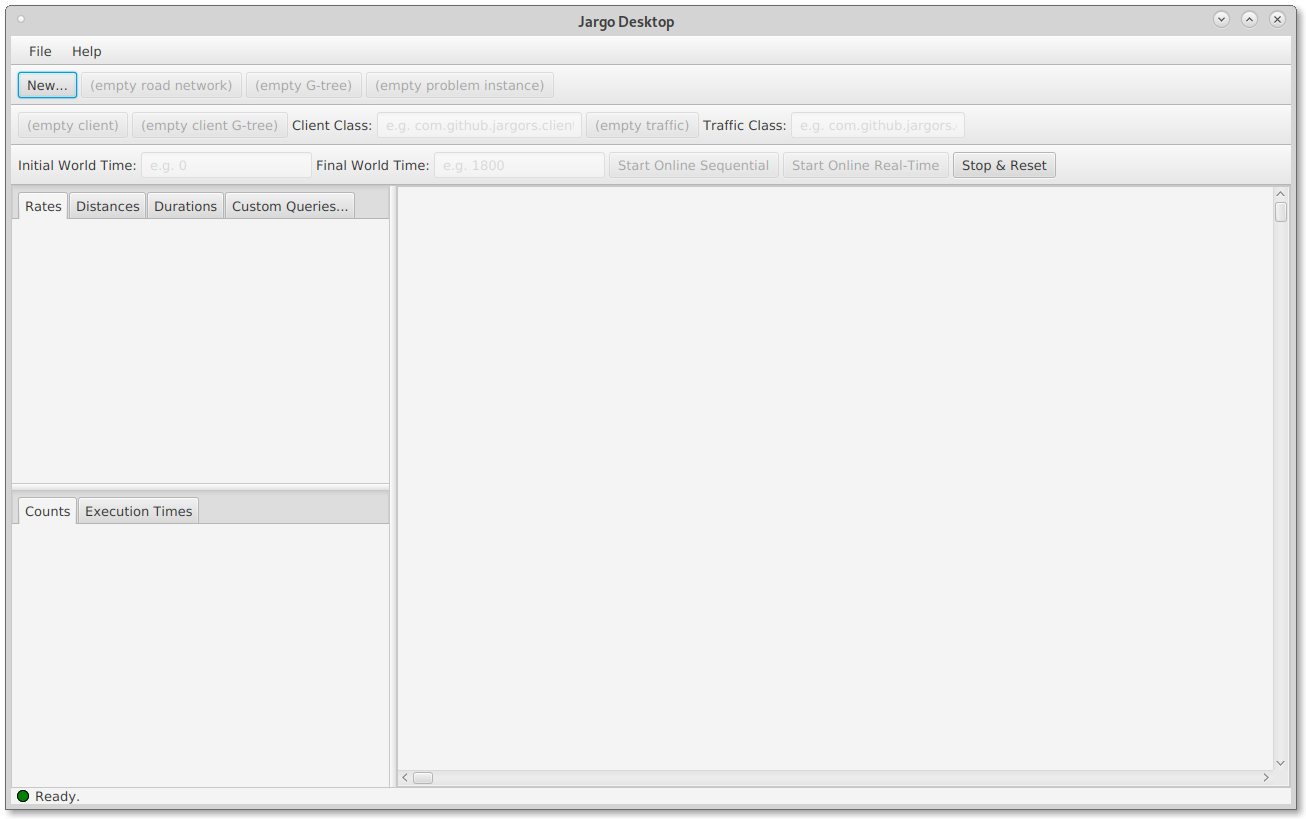
\includegraphics[width=0.8\textwidth]{res/doc-fig/tut-start-gui}
\caption{The graphical evaluator.}
\label{fig:tut-start-gui}
\end{figure}

% \subsection{Writing Your Own Evaluator}
% \label{tut-start: own}
% \emph{Coming soon.}

\begin{table}
\small
\centering
\begin{tabular}{p{.8\textwidth}}
\begin{itemize}
\item jargors-{\jsVersion}.jar
\item commons-logging-1.2.jar
\item \textit{\texttt{derbyclient.jar}}
\item \textit{\texttt{derby.jar}}
\item \textit{\texttt{derbyLocale\_cs.jar}}
\item \textit{\texttt{derbyLocale\_de\_DE.jar}}
\item \textit{\texttt{derbyLocale\_es.jar}}
\item \textit{\texttt{derbyLocale\_fr.jar}}
\item \textit{\texttt{derbyLocale\_hu.jar}}
\item \textit{\texttt{derbyLocale\_it.jar}}
\item \textit{\texttt{derbyLocale\_ja\_JP.jar}}
\item \textit{\texttt{derbyLocale\_ko\_KR.jar}}
\item \textit{\texttt{derbyLocale\_pl.jar}}
\item \textit{\texttt{derbyLocale\_pt\_BR.jar}}
\item \textit{\texttt{derbyLocale\_ru.jar}}
\item \textit{\texttt{derbyLocale\_zh\_CN.jar}}
\item \textit{\texttt{derbyLocale\_zh\_TW.jar}}
\item \textit{\texttt{derbynet.jar}}
\item \textit{\texttt{derbyoptionaltools.jar}}
\item \textit{\texttt{derbyrun.jar}}
\item \textit{\texttt{derbyshared.jar}}
\item \textit{\texttt{derbytools.jar}}
\item \textit{\texttt{derby.war}}
\end{itemize}\\
\end{tabular}

\caption{Additional prerequisites for running Jargo programs.}
\label{tab:tut-start-prerequisites}
\end{table}

\nwenddocs{}\nwfilename{src/tut-analyze.nw}\nwbegindocs{0}\section{Analyzing Results}
\label{tut-analyze}

At the end of each simulation, the command-line and graphical evaluators will
export simulation results to disk for offline analysis. The results are stored
in Derby database format and can be accessed using any tool that supports the
Derby JDBC driver, including the {\Tt{}ij\nwendquote} tool bundled with Derby.

The easiest way to get started is to connect to the database and query Jargo's
SQL views (Table~\ref{tab:tut-analyze-views}). You can use a JDBC connection
string such as {\Tt{}'connect:jdbc:derby:memory:temp;createFrom=jargo'\nwendquote} to connect
to the database, replacing {\Tt{}jargo\nwendquote} with the name of the export. This string
creates a new in-memory Derby database called {\Tt{}temp\nwendquote} and loads the contents
of {\Tt{}jargo\nwendquote} into this database. Use your tool to list the views. In {\Tt{}ij\nwendquote},
the command is {\Tt{}show\ views\nwendquote}.

\begin{table}[h]
\small
\centering
\begin{tabular}{p{.8\textwidth}}
\begin{verbatim}
$ ij
ij version 10.15
ij> connect 'jdbc:derby:memory:temp;createFrom=jargo';
ij> show views;
TABLE_SCHEM         |TABLE_NAME                    |REMARKS
------------------------------------------------------------------------
APP                 |ASSIGNMENTS                   |
APP                 |ASSIGNMENTS_R                 |
APP                 |DIST_BASE                     |
APP                 |DIST_R_BASE                   |
APP                 |DIST_R_DETOUR                 |
APP                 |DIST_R_TRANSIT                |
APP                 |DIST_R_UNASSIGNED             |
APP                 |DIST_S_BASE                   |
APP                 |DIST_S_CRUISING               |
APP                 |DIST_S_SERVICE                |
APP                 |DIST_S_TRAVEL                 |
APP                 |DUR_R_PICKUP                  |
APP                 |DUR_R_TRANSIT                 |
APP                 |DUR_R_TRAVEL                  |
APP                 |DUR_S_SERVICE                 |
APP                 |DUR_S_TRAVEL                  |
APP                 |F_DISTANCE_BLOCKS             |
APP                 |F_STATUS                      |
APP                 |R_SERVER                      |
APP                 |R_USER                        |
APP                 |SERVICE_RATE                  |
APP                 |T_R_ARRIVE                    |
APP                 |T_R_DEPART                    |
APP                 |T_S_ARRIVE                    |
APP                 |T_S_DEPART                    |
APP                 |VIOLATIONS_T_R                |
APP                 |VIOLATIONS_T_S                |

27 rows selected
ij>
\end{verbatim}\\
\end{tabular}

\caption{Listing the Jargo views using \texttt{ij}.}
\label{tab:tut-analyze-views}
\end{table}

\subsection{Assignments}

\subsubsection{\texttt{ASSIGNMENTS}}

This view lists all assignments. Each row consists of the
assigned vehicle and customer along with the time that the assignments was
completed (the customer drop-off time). The {\Tt{}sid\nwendquote} column stores the
vehicle identifier and the {\Tt{}rid\nwendquote} column stores the customer identifier.
See Table~\ref{tab:tut-analyze-assignments} for an example.
Here are some common queries:
\begin{itemize}
\item To get the total number of assignments, use \texttt{SELECT COUNT (rid) FROM ASSIGNMENTS}.
\item To get assignments per vehicle, use \texttt{SELECT sid, COUNT (rid) FROM
ASSIGNMENTS GROUP BY sid}.
\item To get average number of assignments per vehicle, use \texttt{SELECT
CAST(COUNT (rid) / COUNT(DISTINCT (sid)) AS FLOAT) FROM ASSIGNMENTS}.
\end{itemize}

\begin{table}[h]
\small
\centering
\begin{tabular}{p{.8\textwidth}}
\begin{verbatim}
ij> SELECT * FROM ASSIGNMENTS FETCH FIRST 5 ROWS ONLY;
T          |SID        |RID
-----------------------------------
34         |791        |240792
78         |396        |240773
80         |477        |240795
85         |629        |240848
88         |503        |240901

5 rows selected
ij>
\end{verbatim}\\
\end{tabular}

\caption{The \texttt{ASSIGNMENTS} view.}
\label{tab:tut-analyze-assignments}
\end{table}

\subsubsection{\texttt{SERVICE\_RATE}}

This view gives the total ``service rate'' as a percentage multiplied by
$10^4$ (\textit{e.g.} 1.0, or 100\%, is written as 10000). The service
rate is found by dividing the number of assigned customers over the
total number of customers. The total is listed in the \texttt{val} column.

\subsection{Distances}

\subsubsection{\texttt{DIST\_BASE}}

This view lists the total ``base'' distance for all customers and vehicles, in
meters. The base distance for a customer is the shortest travel distance from
the customer's pick-up location to the drop-off location, and for a vehicle is
the shortest travel distance from the vehicle's starting location to the ending
location. The total is listed in the \texttt{val} column.

\subsubsection{\texttt{DIST\_R\_BASE}}

This view lists the total ``base'' distance for all customers only.

\subsubsection{\texttt{DIST\_R\_DETOUR}}

This view lists the ``detour'' distance for each customer, in meters. The
detour distance is found by taking the customer's transit distance and then
subtracting the customer's base distance. The \texttt{rid} column lists the
customer identifier and the \texttt{val} column lists the detour distance. See
Table~\ref{tab:tut-analyze-dist-r-detour} for an example.

\begin{table}[h]
\small
\centering
\begin{tabular}{p{.8\textwidth}}
\begin{verbatim}
ij> select * from dist_r_detour fetch first 5 rows only;
RID        |VAL
-----------------------
51300      |1178
51301      |1384
51302      |854
51303      |1685
51304      |1854

5 rows selected
ij>
\end{verbatim}\\
\end{tabular}

\caption{The \texttt{DIST\_R\_DETOUR} view.}
\label{tab:tut-analyze-dist-r-detour}
\end{table}

\subsubsection{\texttt{DIST\_R\_TRANSIT}}

This view lists the ``transit'' distance for each customer, in meters. The
transit distance is the distance the customer actually traveled by taking a
ridesharing vehicle. The \texttt{rid} column lists the customer identifier and
the \texttt{val} column lists the detour distance.
See Table~\ref{tab:tut-analyze-dist-r-transit} for an example.

\begin{table}[h]
\small
\centering
\begin{tabular}{p{.8\textwidth}}
\begin{verbatim}
ij> select * from dist_r_transit fetch first 5 rows only;
RID        |VAL
-----------------------
51300      |5328
51301      |5242
51302      |1654
51303      |6646
51304      |10356

5 rows selected
ij>
\end{verbatim}\\
\end{tabular}

\caption{The \texttt{DIST\_R\_TRANSIT} view.}
\label{tab:tut-analyze-dist-r-transit}
\end{table}

\subsubsection{\texttt{DIST\_R\_UNASSIGNED}}

This view lists the total ``base'' distance for all \emph{unassigned} customers
only.

\subsubsection{\texttt{DIST\_S\_BASE}}

This view lists the total ``base'' distance for all vehicles only.

\subsubsection{\texttt{DIST\_S\_CRUISING}}

This view lists the ``cruising'' distance for each vehicle, in meters. The
cruising distance is the distance the vehicle traveled while empty (no
customers onboard).

\subsubsection{\texttt{DIST\_S\_SERVICE}}

This view lists the ``service'' distance for each vehicle, in meters. The
service distance is the distance the vehicle traveled while having
customers onboard.

\subsubsection{\texttt{DIST\_S\_TRAVEL}}

This view lists the ``travel'' distance for each vehicle, in meters. The
travel distance is the sum of the service and cruising distances.

\subsection{Durations}

\subsubsection{\texttt{DUR\_R\_PICKUP}}

This view lists the ``pick-up'' duration for each customer, in seconds. The
pick-up duration is the difference between the time a customer is picked up and
the time the customer first appears on the road network.
See Table~\ref{tab:tut-analyze-dur-r-pickup} for an example.

\begin{table}[h]
\small
\centering
\begin{tabular}{p{.8\textwidth}}
\begin{verbatim}
ij> select * from dur_r_pickup fetch first 5 rows only;
RID        |VAL
-----------------------
240764     |36
240765     |107
240766     |31
240767     |45
240768     |33

5 rows selected
ij>
\end{verbatim}\\
\end{tabular}

\caption{The \texttt{DUR\_R\_PICKUP} view.}
\label{tab:tut-analyze-dur-r-pickup}
\end{table}

\subsubsection{\texttt{DUR\_R\_TRANSIT}}

This view lists the ``transit'' duration for each customer, in seconds. The
transit duration is the difference between the time a customer is dropped off
and the time the customer is picked up, in other words the time a customer
spends inside a vehicle.
See Table~\ref{tab:tut-analyze-dur-r-transit} for an example.

\begin{table}[h]
\small
\centering
\begin{tabular}{p{.8\textwidth}}
\begin{verbatim}
ij> select * from dur_r_transit fetch first 5 rows only;
RID        |VAL
-----------------------
240764     |139
240765     |163
240766     |242
240767     |1075
240768     |380

5 rows selected
ij>
\end{verbatim}\\
\end{tabular}

\caption{The \texttt{DUR\_R\_TRANSIT} view.}
\label{tab:tut-analyze-dur-r-transit}
\end{table}

\subsubsection{\texttt{DUR\_R\_TRAVEL}}

This view lists the ``travel'' duration for each customer, in seconds. The
travel duration is the difference between the time a customer is dropped off
and the time the customer appears on the road network, in other words the
sum of the pick-up and transit durations.
See Table~\ref{tab:tut-analyze-dur-r-travel} for an example.

\begin{table}[h]
\small
\centering
\begin{tabular}{p{.8\textwidth}}
\begin{verbatim}
ij> select * from dur_r_travel fetch first 5 rows only;
RID        |VAL
-----------------------
240764     |175
240765     |270
240766     |273
240767     |1120
240768     |413

5 rows selected
ij>
\end{verbatim}\\
\end{tabular}

\caption{The \texttt{DUR\_R\_TRAVEL} view.}
\label{tab:tut-analyze-dur-r-travel}
\end{table}

\subsubsection{\texttt{DUR\_S\_SERVICE}}

This view lists the ``service'' duration for each vehicle, in seconds. The
service duration is the time spent with customers onboard.

\subsubsection{\texttt{DUR\_S\_TRAVEL}}

This view lists the ``travel'' duration for each vehicle, in seconds. The
travel duration is the total time spent traveling on the road network.

\subsection{Other Views}

\subsubsection{\texttt{F\_DISTANCE\_BLOCKS}}

This view lists the departure load on each vehicle for each location the
vehicle visits. It is used to determine service and cruising distances.

\subsubsection{\texttt{F\_STATUS}}

This view lists the ``status'' of each assigned customer after pick-up and
after drop-off. It is used to determine the assignments.

\subsubsection{\texttt{R\_SERVER}}

This view lists each vehicle location and the ``events'' that took place on
those locations. See Section~\ref{user-mod: server-relation} for more
information.

\subsubsection{\texttt{R\_USER}}

This view lists each vehicle and customer along with their properties.
See Section~\ref{user-mod: user-relation} for more information.

\subsubsection{\texttt{T\_R\_ARRIVE}}

This view lists drop-off times for each customer.

\subsubsection{\texttt{T\_R\_DEPART}}

This view lists pick-up times for each customer.

\subsubsection{\texttt{T\_S\_ARRIVE}}

This view lists arrival times for each vehicle.

\subsubsection{\texttt{T\_S\_DEPART}}

This view lists departure times for each vehicle.

\subsubsection{\texttt{VIOLATIONS\_T\_R}}

This view lists the amount of the ``time window violation'' for each customer.
This amount is found by taking the drop-off time and subtracting the latest
acceptable drop-off time for the customer.

\subsubsection{\texttt{VIOLATIONS\_T\_S}}

This view lists the amount of the ``time window violation'' for each vehicle.

\nwenddocs{}\nwfilename{src/mod-setting.nw}\nwbegindocs{0}\chapter{Ridesharing Model}
\label{ch-model}

Physical concepts, such as customers, vehicles, and ridesharing service-related
metrics, are defined on Jargo's data tables using relational and set algebra.
For a primer on relations and notes on notation used in this document, see
Appendix~\ref{ap-primer}.

\section{Ridesharing Setting}
\label{mod-setting}

This section describes Jargo's model for the ridesharing setting.

\subsection{Time}
\label{mod-setting: time}

Time is modeled as a positive integer $1\leq t\leq H$. A time horizon $H$
bounds the system. Time can be operated on. Times cannot be added, but a later
(greater) time can subtract an earlier (lesser) time. The difference is called
a duration, represented by the symbol $\delta$. Durations can add and subtract
each other to get new durations, and times can also add and subtract durations
to get new times.

\subsection{Road Network}
\label{mod-setting: road}

The road network is modeled as a directed graph
$\mathcal{G}(\mathcal{V},\mathcal{E})$. Vertices in $\mathcal{V}$ represent
points along roads in the network.  A function ${V:\mathcal{V}\rightarrow
\mathbb{R}^2}$ maps vertices to $2$-dimensional latitude and longitude
coordinates in the real world, and an inverse function map-matches customers
and vehicles to vertices. Edges in $\mathcal{E}$ represent road segments. The
pair $(a,b)\in \mathcal{V}^2, a\neq b$ exists in $\mathcal{E}$ only if physical
traffic flows from $V(a)$ to $V(b)$, and for all $c\in
\mathcal{V}\setminus\{a,b\}$ no traffic flows from $V(a)$ to $V(c)$ and from
$V(c)$ to $V(b)$. A function ${d:\mathcal{E}\rightarrow\mathbb{R}_{>0}}$ maps
edges to positive real weights corresponding to distance along the edge, and
the shortest-path distances between the pairs among any three vertices
satisfies the triangle inequality. Figure~\ref{fig:road} shows an example road
network, drawn in QGIS, that could be supported by Jargo's model.

\begin{figure}[h]
\centering
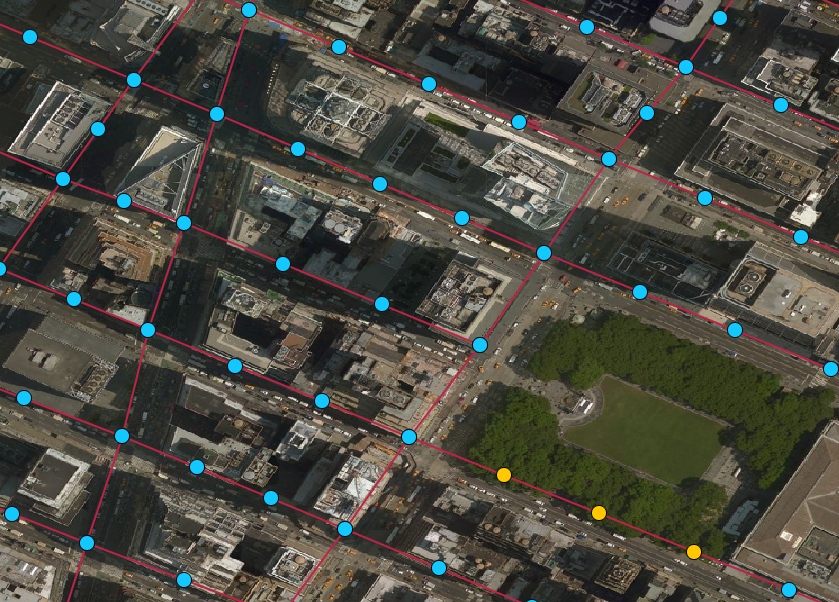
\includegraphics[width=0.8\textwidth]{res/doc-fig/road}
\caption{Portion of a road network graph showing edges (red lines) and vertices
(blue circles) overlayed on top of Manhattan (QGIS 2.18.16, Bing Aerial).
Vertices do not have to be at an intersection (orange circles, lower right).}
\label{fig:road}
\end{figure}

\subsection{Paths}
\label{mod-setting: paths}

A path $p=(p_i)_{i\in 1..n}=p_1..p_n$ is defined as a sequence of $n$ vertices
such that any two adjacent vertices are an edge, or $(p_i,p_{i+1})\in
\mathcal{E}$ for $i\in 1..(n-1)$.  A vertex or edge can appear multiple times
in a path.  The path distance is $$\sum_{i=1}^{n-1} d(p_i, p_{i+1}).$$ Path $p$
is a shortest path only if it minimizes the distance out of all possible paths
from $p_1$ to $p_n$.  Multiple shortest paths are possible.

\subsection{Waypoints}
\label{mod-setting: waypoints}

Waypoints are used to describe points in time as well as space.  A waypoint is
defined as a tuple $(\texttt{t},\texttt{v})$, with the domain of $\texttt{t}$
as $1..H$ and the domain of $\texttt{v}$ as $\mathcal{V}$. Waypoints can be
labeled in a way that will be discussed later.

\subsection{Routes}
\label{mod-setting: routes}

Routes are formed by a sequence of waypoints. A route $w=(w_i)_{i\in
1..n}=w_1..w_n=(t_1,v_1)..(t_n,v_n)$ is defined as a sequence of $n$ waypoints
such that $t_1..t_n$ is strictly increasing and $v_1..v_n$ is a path.  In the
spatial dimension, function
$$D(w)=\sum_{i=1}^{n-1}d(\pi_\texttt{v}(w_i),\pi_\texttt{v}(w_{i+1}))$$ gives
the route distance, analogous to path distance.  In the time dimension,
function $$\delta(w)=\pi_\texttt{t}(w_n)-\pi_\texttt{t}(w_1)$$ gives the route
duration.  Given a time $t$, \begin{align*} w_{\leq
t}=\textrm{sort}(\sigma_{\texttt{t}\leq t}(w))\quad\textrm{and}\quad
w_{>t}=\textrm{sort}(\sigma_{\texttt{t}>t}(w)) \end{align*} give the traveled
route denoted $w_{\leq t}$, and the remaining route denoted $w_{>t}$. As the
selection operator imposes no ordering on the resulting set, a
$\textrm{sort}(...)$ function is introduced to sort a set of waypoints by time
in ascending order, returning a sequence.  For two adjacent waypoints $w_i$
and~$w_{i+1}$, function
$$\nu(w_i,w_{i+1})=\frac{d(\pi_\texttt{v}(w_i),\pi_\texttt{v}(w_{i+1}))}
{\pi_\texttt{t}(w_{i+1})-\pi_\texttt{t}(w_i)}$$ gives the waypoint rate, or
more intuitively the speed.  As $d$ only applies to edges, $\nu$ only applies
to adjacent waypoints.  Speeds can be bounded above by a value
$\nu^\textrm{max}(v_i,v_{i+1})$ on each edge, for example to describe road
speed limits.

\nwenddocs{}\nwfilename{src/mod-users.nw}\nwbegindocs{0}\section{Ridesharing Users}
\label{mod-users}

In Jargo, the basic entity representing a ridesharing participant is the
\emph{user}.  Table~\ref{tab:mod-users-types} describes the types of users
recognized by Jargo, and Table~\ref{tab:mod-users-properties} describes their
properties.  Table~\ref{tab:mod-users-rules} describes rules governing their
behavior.  A user is classified as a \emph{request} if it represents a Type~1
or Type~2 customer, or classified as a \emph{server} if it represents a Type~3
or Type~4 vehicle. As only vehicles can move about (P4), only servers are
associated with routes in order to describe the motions. Later, schedules
describing pick-up and drop-off events are defined on the routes.

\begin{table}[h]
\centering
\small
\begin{tabular}{|l|l|}
\hline Type   & Description \\
\hline
Type 1 & Single customer traveling alone \\
Type 2 & Group of customers traveling together \\
\hline
Type 3 & Ridesharing vehicle with a predefined final
    destination \\
Type 4 & Taxi-like vehicle continually serving customers without an
    explicit destination of its own \\
\hline
\end{tabular}

\caption{Types of ridesharing users.}
\label{tab:mod-users-types}

\begin{tabular}{|c|p{140mm}|}
\hline
Prop. & Description \\
\hline
P1 & \hi{Load.} Each user has a non-zero load, indicating a
number of needed seats. For Type 1 users the load is 1, indicating they only
need a single seat. For Type 2 users the load exceeds 1. For Type 3 and Type 4
users the load is negative, indicating they have an availability of seats. \\
\hline
P2 & \hi{Origin and Destination.} Each user has an origin and a
destination, except for Type 4 users that only have an origin.  For Type
1 and Type 2, the origin indicates the initial location of the customer
and the destination indicates the desired final location.  For Type 3, the
origin and destination indicate where the vehicle's ridesharing service begins
and ends.\\
\hline
P3 & \hi{Time Window.} Each user has an early time and a
late time, together forming the user's time window. For a Type 1
or Type 2 customer, the time window gives the desired departure time from the
origin and the desired arrival time at the destination.  For a Type 3 or Type 4
vehicle, the time window gives the time when service begins and the latest time
that service can end. The early time precedes the late time.\\
\hline
\end{tabular}

\caption{Ridesharing user properties.}
\label{tab:mod-users-properties}

\begin{tabular}{|c|p{140mm}|}
\hline
Prop. & Description \\
\hline
P4 & \hi{Motion.} Users are bound to a network of roads, for
example the streets of a city. Only vehicles may directly travel along the
roads, whereas customers must be serviced by a vehicle. Both customers and
vehicles may enter the system at any time and anywhere.\\
\hline
P5 & \hi{Pick-ups and Drop-offs.} For a vehicle to service a customer, it
must first travel to the customer's origin to pick up the customer, and then to
the customer's destination to drop off the customer, in that order. The
customer enters the vehicle during the pick-up and exits the vehicle during the
drop-off. These visits must occur within the customer's time window.\\
\hline
P6 & \hi{Vehicle Seats.} When a customer enters a vehicle, the customer
occupies a number of seats equal to the customer's load. When it exits the
vehicle, it relinquishes the seats. At no time can the number of occupied seats
exceed the number of available seats in a vehicle.\\
\hline
P7 & \hi{User States.} A customer can be in one of three states at any
time: waiting for pick-up; in-transit following a pick-up but
before the drop-off; or arrived at destination. A vehicle can be either
in-service or out-of-service.\\
\hline
\end{tabular}

\caption{Rules governing user behavior.}
\label{tab:mod-users-rules}
\end{table}

\subsection{User Relation}
\label{mod-users: user-relation}

A user $u$ is a 5-tuple defined by
${u:=(\texttt{q},\texttt{e},\texttt{l},\texttt{o},\texttt{d})}$.  The
\texttt{q} component corresponds to the user load; the \texttt{e} and
\texttt{l} components correspond to the user early and late times; the
\texttt{o} and \texttt{d} components correspond to the user origin and
destination.  From P1--P4, the domain of \texttt{q} is the non-zero integers;
the domain of \texttt{e} is $1..(H-1)$ and the domain of \texttt{l} is
$(u_\texttt{e}+1)..H$; the domains of \texttt{o} and \texttt{d} are both
$\mathcal{V}$.  For a Type 4 vehicle, the destination can be set to a dummy
vertex with edge weight equal to 0 to every other vertex in the road network.

The set of all users forms the 5-ary relation $\mathcal{U}$, called the user
relation.  The set $\mathcal{U}_\texttt{o}=\pi_\texttt{o}(\mathcal{U})$
contains all origins and $\mathcal{U}_\texttt{d}=\pi_\texttt{d}(\mathcal{U})$
contains all destinations.  From P1, a user can be classified as either a
request or a server based on its load.

As a convenience, the notation $d_u$ is used to denote the distance of the
shortest path from $u_\texttt{o}$ to $u_\texttt{d}$ on graph $\mathcal{G}$, and
the notation $\delta_u$ is used to denote the shortest travel duration along
$d_u$ using the speed limits $\nu^\textrm{max}$ along the shortest-path edges.

\subsection{Requests}
\label{mod-users: requests}

A request represents a Type 1 or Type 2 customer.  Relation
$\mathcal{R}\subseteq\mathcal{U}$,
$$\mathcal{R}=\sigma_{\texttt{q}>0}(\mathcal{U}),$$ forms the set of all
requests by taking users with positive loads. The set
$\mathcal{R}_\texttt{o}=\pi_\texttt{o}(\mathcal{R})$ is the set of all request
origins and $\mathcal{R}_\texttt{d}=\pi_\texttt{d}(\mathcal{R})$ is the set of
all request destinations.

\subsection{Servers}
\label{mod-users: servers}

Likewise, a server represents a Type 3 or Type 4 vehicle.  Relation
$\mathcal{S}=\mathcal{U}\setminus\mathcal{R}$, or
$$\mathcal{S}=\sigma_{\texttt{q}<0}(\mathcal{U}),$$ forms the set of all
servers. The set $\mathcal{S}_\texttt{o}=\pi_\texttt{o}(\mathcal{S})$ is the
set of all server origins and
$\mathcal{S}_\texttt{d}=\pi_\texttt{d}(\mathcal{S})$ is the set of all server
destinations.

\subsection{Routes}
\label{mod-users: routes}

To encode vehicle motions, Jargo associates each server $s\in\mathcal{S}$ with
a route and a schedule. A server's route is a representation of the
corresponding vehicle's motion through the road network while a server's
schedule encodes the times and locations of customer pick-ups and drop-offs.

Variable $w$ indicates the route for a server $s$. As time advances, the
traveled route $w_{\leq t}$ encodes the server's past motion while the
remaining route $w_{>t}$ encodes the future motion.  From P2 and P3, Jargo
subjects all routes to two rules:
\begin{enumerate}
\item[R1.] The time component of the first waypoint equals the server's early
time, and the time component of the last waypoint is not greater than the
server's late time, or $\pi_\texttt{t}(w_1)=s_\texttt{e}$ and
$\pi_\texttt{t}(w_{|w|})\leq s_\texttt{l}$;
\item[R2.] The vertex components of the first and last waypoints equal the
server's origin and destination respectively, or
$\pi_\texttt{v}(w_1)=s_\texttt{o}$ and $\pi_\texttt{v}(w_{|w|})=s_\texttt{d}$.
\end{enumerate}

\subsection{Schedules}
\label{mod-users: schedules}

A server's schedule describes the events along the route and not any new
motion. It is a subsequence of the server's route $w$
$$b=(b_j)_{j\in 1..m}=(w_{i_j})_{j\in 1..m}=(t_{i_1},v_{i_1})..(t_{i_m},v_{i_m}),$$
with $m\leq |w|$ waypoints. Schedules are subjected to a couple rules. First:
\begin{enumerate}
\item[R3.] The first and last waypoints $b_1$ and $b_m$ equal the first and last
waypoints of $w$, or ${b_1=w_1}$ and ${b_m=w_{|w|}}$.
\end{enumerate}
This rule will help later when defining departure and arrival times.
Second, from P5:
\begin{enumerate}
\item[R4.] For each waypoint $b_j$ for $j\in 2..(m-1)$, the vertex component is either a
request origin or request destination, or $\pi_\texttt{v}(b_j)\in
\mathcal{R}_\texttt{o}\cup\mathcal{R}_\texttt{d}$.
\end{enumerate}
In other words, each entry or exit must occur at a customer origin or
destination.

A schedule formalizes the notion of shared travel with other users, as multiple
entries and exits can overlap within the same server route.  At time $t$, the
traveled schedule denoted $b_{\leq t}$ encodes the past entries and exits and
is given by $\sigma_{\texttt{t}\leq t}(b)$. Likewise, the remaining schedule
denoted $b_{>t}$ encodes the future entries and exits and is given by
$\sigma_{\texttt{t}>t}(b)$.

\subsection{Schedule Labels}
\label{mod-users: labels}

Each waypoint in schedule $b$ has a set of labels in order to identify which
customers are entering and exiting the vehicle at the waypoint's time and
location.  A labeling scheme can be applied to $b$ to determine each of the
labels. The set of all possible labels depends on the locations of the
waypoints. Let
$$\mathcal{R}'=\sigma_{\texttt{o}\in\pi_\texttt{v}(b)\lor \texttt{d}\in\pi_\texttt{v}(b)}(\mathcal{R})$$
give the set of requests whose origin or destination is found in at least one
waypoint in $b$. Conceptually, the labeling scheme
\begin{equation*}
L:b\rightarrow \mathbb{P}(\mathcal{R}'\cup\{s\})
\end{equation*}
maps elements of $b$ to elements of the power set of $\mathcal{R}'\cup\{s\}$.
By using the power set $\mathbb{P}$, a waypoint can have multiple labels,
representing the case where multiple customers enter or exit the vehicle at the
waypoint.  The labeling scheme is subjected to the following labeling rules:
\begin{enumerate}
\item[R5.] No waypoint can be labeled with $r\in\mathcal{R}'$ if a schedule for
another server already contains waypoints labeled with $r$;
\item[R6.] A waypoint $b_j\in b$ can be labeled with $r$ only if
$\pi_\texttt{v}(b_j)=r_\texttt{o}$ or $\pi_\texttt{v}(b_j)=r_\texttt{d}$;
\item[R7.] If $b_j$ is to be labeled with $r$ and
$\pi_\texttt{v}(b_j)=r_\texttt{o}$, then a second waypoint $b_{j'}$ such that
$j'>j$ and $\pi_\texttt{v}(b_{j'})=r_\texttt{d}$ must also be labeled with $r$;
\item[R8.] The time components of $b_j$ and $b_{j'}$ must be within request
$r$'s time window, formally $r_\texttt{e}\leq \pi_\texttt{t}(b_j)$ and
$\pi_\texttt{t}(b_{j'})\leq r_\texttt{l}$;
\item[R9.] The number of waypoints labeled with $r$ must be exactly 0 or 2;
\item[R10.] The first and last waypoints must contain the schedule's server $s$
in their labels, and no other waypoint can be labeled with $s$.
\end{enumerate}
Rules R5--R9 express P5.  Rule R10 can be interpreted to mean that a vehicle
must ``serve itself'' at its own origin and destination.  This last rule helps
to define later concepts.

\subsection{Server Relation}
\label{user-mod: server-relation}

By combining the routes, schedules, and labels into a set of
$(\texttt{s},\texttt{t},\texttt{v},\texttt{L})$ tuples, a 4-ary relation
$\mathcal{X}$ can be formed. Jargo calls this relation the server relation.
Each tuple associates the waypoint in the \texttt{t} and \texttt{v} components
with the server in the \texttt{s} component, along with the labels in the
\texttt{L} component.

A server's route can be recovered by extracting \texttt{t} and \texttt{v}
components and sorting by time, or formally for a given server $s$, its route
is given by
$$W(\mathcal{X},s)=\textrm{sort}(\pi_{\texttt{t},\texttt{v}}(\sigma_{\texttt{s}=s}(\mathcal{X}))).$$
Similarly, a server's schedule can be recovered by extracting only those
waypoints that are labeled, formally
$$B(\mathcal{X},s)=\textrm{sort}(\pi_{\texttt{t},\texttt{v}}(\sigma_{\texttt{s}=s\land |\texttt{L}|>0}(\mathcal{X}))).$$

The server relation can be used to define the remaining physical concepts, P6 and P7.

\subsection{Request Status}
Given a request $r$, the function
\begin{equation}
\label{eq:status}
\textrm{status}(\mathcal{X},r,t)=|\sigma_{\texttt{t}\leq t\land
r\in\texttt{L}}(\mathcal{X})|
\end{equation}
gives the count of the tuples labeled with $r$ before or on a given time. From
the labeling rules, the count can be only 0, 1, or 2. These counts correspond
to request waiting, in-transit, and arrived states from P7, respectively.

Given a server $s$, knowing the in-transit requests for $s$ can be useful for
pricing and other rider-related
metrics. %~\cite{DBLP:conf/sigmod/ChengX017,DBLP:conf/dexa/ShiLZG17,DBLP:conf/ijcai/SantosX13}.
These requests can be found by
$$\mathcal{Q}(\mathcal{X},s,t)=\{r\in\mathcal{R}\mid\textrm{status}(\mathcal{X},r,t)=1
\land\pi_\texttt{s}(\sigma_{r\in\texttt{L}}(\mathcal{X}))=s\}.$$

\subsection{Load Burden}
The load burden on $s$ can be computed using the in-transit requests by
\begin{equation}
\label{eq:load}
Q(\mathcal{X},s,t)=\sum_{r\in\mathcal{Q}(\mathcal{X},s,t)}r_\texttt{q}.
\end{equation}
From P6, server routes are subject to the additional rule:
\begin{enumerate}
\item[R11.] $Q(\mathcal{X},s,t)\leq -s_\texttt{q}$ must be true for all $s$ and $t$.
\end{enumerate}

\nwenddocs{}\nwfilename{src/mod-metrics.nw}\nwbegindocs{0}\section{Ridesharing Metrics}
\label{mod-metrics}

A variety of metrics can be measured by simple operations on $\mathcal{U}$ and
$\mathcal{X}$. This section lists those that have been implemented in Jargo.

\subsection{Assignments}
\label{mod-metrics: assignments}

Server $s$ is said to be assigned to request $r$ at time $t$ only if
$\textrm{status}(\mathcal{X},r,t)=2$. That is, the request's status is arrived
at time $t$. The set of $(s,r)$ pairs where this property is true is called
the set of assignments, formally
\begin{equation}
\label{eq:assignments}
\textit{assignments }A(\mathcal{X},t)=
\{(s,r)\in\mathcal{S}\times \mathcal{R} \mid \textrm{status}(\mathcal{X},r,t)=2\}.
\end{equation}
Using the assignments,
\begin{align}
\label{eq:assigned-requests}
\textit{assigned requests }R^\textrm{ok}(\mathcal{X},t)&=\pi_\texttt{r}(A(\mathcal{X},t))\textrm{, and}\\
\label{eq:unassigned-requests}
\textit{unassigned requests }R^\textrm{ko}(\mathcal{X},t)&=\mathcal{R}\setminus\mathcal{R}^\textrm{ok}(\mathcal{X},t).
\end{align}
The server assigned to $r$ can be obtained with
\begin{equation}
S(\mathcal{X},r,t)=\{s\in\mathcal{S}\mid\textrm{status}(\mathcal{X},r,t)=2\},
\end{equation}
guaranteed to return only one server due to R5.
Likewise, the set of requests assigned to $s$ can be obtained with
\begin{equation}
\label{eq:R(X,s,t)}
R(\mathcal{X},s,t)=\{r\in\mathcal{R}\mid\textrm{status}(\mathcal{X},r,t)=2\}.
\end{equation}

\subsection{Service Rate}
\label{mod-metrics: service-rate}
The service rate is the number of assigned requests over the number of all requests, or
\begin{equation}
\label{eq:service-rate}
\textit{service rate }\mu(\mathcal{X},t)=\frac{|R^\textrm{ok}(\mathcal{X},t)|}{|\mathcal{R}|}.
\end{equation}

\subsection{Distances}
\label{mod-metrics: distances}

The base distance is the sum of the shortest-path distances for all users, or
\begin{equation}
\label{eq:base-distance}
\textit{base distance }D^\textrm{base}(\mathcal{U})=\sum_{u\in U}d_u.
\end{equation}
The travel distance for one server $s$ is the distance of its route,
$D(W(\mathcal{X},s))$,
and the travel duration can be found with
$\delta(W(\mathcal{X},s))$.

For a server with route $w$, travel distance $D(w)$ can be partitioned into
cruising distance $D_0(w)$ and
service distance $D_1(w)$.
The cruising distance sums the distance along portions where the load burden is zero.
The service distance sums the distance along portions of $w$ where the
load burden is non-zero.
Formally, partition $w$ into a set of substrings $\Omega(w)$ such that each waypoint
in $w$ is a member of exactly one substring and that for all substrings $\omega\in \Omega$,
\begin{align}
\label{eq:slack}\textrm{either }Q(\mathcal{X},s,t)&=0\textrm{ is true for all }t\in \pi_\texttt{t}(\omega),\\
\label{eq:block}\textrm{or }Q(\mathcal{X},s,t)&>0\textrm{ is true for all }t\in \pi_\texttt{t}(\omega).
\end{align}
The equations can be used to partition $\Omega(w)$ into two subsets,
\begin{align*}
\Omega_0(w)&=\{\omega\in \Omega(w)\mid \omega\textrm{ satisfies Eq.~\ref{eq:slack}}\}\textrm{ and }\\
\Omega_1(w)&=\{\omega\in \Omega(w)\mid \omega\textrm{ satisfies Eq.~\ref{eq:block}}\}.
\end{align*}
The distances of each of the substrings in each subset can be summed
to get
$$D_0(w)=\sum_{\omega\in \Omega_0(w)} D(\omega)\quad\textrm{and}\quad
  D_1(w)=\sum_{\omega\in \Omega_1(w)} D(\omega).$$
These distances are written as
\begin{align}
\label{eq:cruising-distance}
\textit{cruising distance }D^\textrm{cruise} (\mathcal{X},s)&=D_0(W(\mathcal{X},s)),\textrm{ and}\\
\label{eq:service-distance}
\textit{service distance } D^\textrm{service}(\mathcal{X},s)&=D_1(W(\mathcal{X},s)).
\end{align}

\subsection{Detours and Delays}
\label{mod-metrics: delays}

In physical terms, the detour route for a customer is the portion of a vehicle's
route between when it visits the customer's origin and destination. Formally, let
$w=W(\mathcal{X},S(\mathcal{X},r,H))$ be the route of the server assigned to $r$.
The detour route $\Delta W(\mathcal{X},r)$ is an $m$-length substring of $w$ given by
$\Delta W(\mathcal{X},r)=w_{1+k}..w_{m+k}$ such that for some $k$,
\begin{itemize}
\item $\Delta W(\mathcal{X},r)$ begins at $r_\texttt{o}$, or $\pi_\texttt{v}(w_{1+k})=r_\texttt{o}$,
\item $\Delta W(\mathcal{X},r)$ ends at $r_\texttt{d}$, or $\pi_\texttt{v}(w_{m+k})=r_\texttt{d}$, and
\item the first and last waypoints of $\Delta W(\mathcal{X},r)$ are labeled with $r$, or $r\in\pi_\texttt{L}(w_{1+k})\cap\pi_\texttt{L}(w_{m+k})$.
\end{itemize}
Observe that due to the labeling rules, only one value of $k$ can satisfy these
conditions. The first and last waypoints $w_{1+k}$ and $w_{m+k}$ can be found by
the equations on users,
\begin{align}
\label{eq:pickup}
\textrm{pickup}(\mathcal{X},u)&=\pi_{\texttt{t},\texttt{v}}(\sigma_{\texttt{v}=u_\texttt{o}\land u\in\texttt{L}}(\mathcal{X}))\textrm{, and}\\
\label{eq:dropoff}
\textrm{dropoff}(\mathcal{X},u)&=\pi_{\texttt{t},\texttt{v}}(\sigma_{\texttt{v}=u_\texttt{d}\land u\in\texttt{L}}(\mathcal{X})),
\end{align}
by substituting $r$ for $u$.
Note that if a server is substituted for $u$, these equations give the start and
end waypoints of the server's route due to R3 and R10.
These two equations can also be used to give two times for
any user,
\begin{align}
\label{eq:departure-time}
\textit{departure time }t^\textrm{depart}(\mathcal{X},u)&=\pi_\texttt{t}(\textrm{pickup}(\mathcal{X},u))\textrm{, and}\\
\label{eq:arrival-time}
\textit{arrival time }t^\textrm{arrive}(\mathcal{X},u)&=\pi_\texttt{t}(\textrm{dropoff}(\mathcal{X},u)).
\end{align}
In the real world, the time until a vehicle picks up a customer can be of interest.
This pick-up delay can be found with
\begin{equation}
\label{eq:pick-up delay}
\textit{pick-up delay }\delta^\textrm{pickup}(\mathcal{X},r)=\pi_\texttt{t}(\textrm{pickup}(\mathcal{X},r))-r_\texttt{e}.
\end{equation}

The detour route $\Delta W(\mathcal{X},r)$ can only apply to assigned requests. If
a detour route exists, then
the transit distance and duration are
\begin{align}
\label{eq:transit-distance}
\textit{transit distance }D^\textrm{transit}(\mathcal{X},r)&=D(\Delta W(\mathcal{X},r))\textrm{, and}\\
\label{eq:transit-duration}
\textit{transit duration }\delta^\textrm{transit}(\mathcal{X},r)&=\delta(\Delta W(\mathcal{X},r)).
\end{align}
Similarly, the detour distance and duration are
\begin{align}
\label{eq:detour-distance}
\textit{detour distance }D^\textrm{detour}(\mathcal{X},r)&=D^\textrm{transit}(\mathcal{X},r)-d_r\textrm{, and}\\
\label{eq:detour-duration}
\textit{detour duration }\delta^\textrm{detour}(\mathcal{X},r)&=\delta^\textrm{transit}(\mathcal{X},r)-\delta_r.
\end{align}
Finally, the travel duration is the sum of the pick-up and transit durations,
\begin{equation}
\label{eq:travel-duration}
\textit{travel duration }\delta^\textrm{travel}(\mathcal{X},r)=\delta^\textrm{pickup}(\mathcal{X},r)+\delta^\textrm{transit}(\mathcal{X},r)
=\pi_\texttt{t}(\textrm{dropoff}(\mathcal{X},r))-r_\texttt{e}.
\end{equation}

\subsection{Utilization}
\label{mod-metrics: utilization}

The percentage of servers that are assigned to at least one request is given by
\begin{equation}
\label{eq:server-utilization}
\textit{server utilization }\rho^\textrm{server}(\mathcal{X})=\frac{|\pi_\texttt{s}(\mathcal{A}(\mathcal{X}))|}{|\mathcal{S}|}.
\end{equation}
The distance utilization is
\begin{equation}
\label{eq:distance-utilization}
\textit{distance utilization }\rho^\textrm{distance}(\mathcal{X})=
\frac{\sum_{s\in\mathcal{S}}D^\textrm{service}(\mathcal{X},s)}
{\sum_{s\in\mathcal{S}}D(\mathcal{X},s)}.
\end{equation}

\nwenddocs{}\nwfilename{src/mod-schema.nw}\nwbegindocs{0}\section{SQL Schema}
\label{mod-schema}

The simple constraints allowed by the SQL standard\footnote{ISO/IEC 9075}
(\texttt{CHECK}, \texttt{UNIQUE}, \texttt{NOT NULL}, \texttt{FOREIGN KEY}) are
unable to express the complex ridesharing properties and rules, and
consequently a direct ``translation'' of the ridesharing relations into SQL is
not possible without either making code extensions to SQL or reorganizing the
relational ridesharing model.

Jargo implements the following schema entirely in standard SQL without any code
extensions while staying faithful to the model. In this schema, \textit{tables}
capture the descriptive elements of the model and \textit{views} express the
analytical measures. Tables are further organized into property, solution, and
constraint tables. Property tables store the road network $\mathcal{G}$ and the
user relation $\mathcal{U}$.  Solution tables store the server relation
$\mathcal{X}$.  Constraint tables store copies of data from other tables for
validation purposes.  The views are mostly defined on the constraint tables.

Diagrams of the SQL tables are included in this chapter. In the diagrams,
primary keys are indicated in italics. Elsewhere, column names are
distinguished by \textsf{sans serif} script.  Parentheses are used to logically
group together columns.  A parent table next to a group of columns indicates
foreign key. In SQL, foreign keys must reference their values from the primary
key of the parent table. Many of the table diagrams contain duplicate columns
(for example, \textsf{sid} shows up three times in Table W).  These duplicates
are included for illustrating the foreign key relationships, but in practice
the duplicates are implemented as single columns participating in multiple
foreign keys.

This section also includes Java code chunks. Double-angle brackets enclose the
chunk name, used to refer to the chunk in other parts of the document.
Anything after the equals sign and before the ``at'' sign is live code. Noweb
is used to compile the code chunks into correct Java source code.

\subsection{Road Network Tables (Tables V and E)}
\label{mod-schema: road}

Each vertex $v\in\mathcal{V}$ is stored in Table V along with its coordinates
$V(v)$ while each edge $(a,b)\in\mathcal{E}$ is stored in Table E along with
its weight $d(a,b)$ and speed limit $\nu^\textrm{max}(a,b)$.  Table V thus has
three columns, storing $v$ in primary key column \textsf{v} ({\Tt{}P1\nwendquote}) and its
coordinates in column \textsf{lng} and \textsf{lat}.  Likewise, Table E has
four columns, storing $a$ and $b$ in column \textsf{v1} and \textsf{v2},
$d(a,b)$ in column \textsf{dd}, and $\nu^\textrm{max}(a,b)$ in column
\textsf{nu}.  The four columns together form the primary key ({\Tt{}P2\nwendquote}) in order
to be referenced by later tables.  Foreign keys on \textsf{v1} ({\Tt{}F1\nwendquote}) and
\textsf{v2} ({\Tt{}F2\nwendquote}) referencing Table V validate that $a$ and $b$ are actual
vertices.
\begin{table}[h]
\centering
\small
\begin{tabular}{|c|l|}
\hline
\rowcolor{TableTitle}
\multicolumn{2}{|c|}{Table V (Vertices)}\\
\hline
\rowcolor{TableHeader}
Column & Description\\
\hline
\textit{v} & Vertex $v\in\mathcal{V}$\\
\hline
lng & \multirow{2}{*}{Vertex coordinate $V(v)$}\\
lat & \\
\hline
\end{tabular}

\begin{tabular}{|c|c|l|}
\hline
\rowcolor{TableTitle}
\multicolumn{3}{|c|}{Table E (Edges)}\\
\hline
\rowcolor{TableHeader}
Column & Parent & Description\\
\hline
\textit{v1} & Table V & \multirow{2}{*}{Edge $(a, b)\in\mathcal{E}$} \\
\cline{2-2}
\textit{v2} & Table V & \\
\hline
\textit{dd} & & Weight $d(a,b)$\\
\hline
\textit{nu} & & Max. speed $\nu^\textrm{max}(a,b)$\\
\hline
\end{tabular}
\end{table}

Jargo considers vertex 0 to be a dummy vertex where any edged formed by 0 has
no weight. To implement the dummy vertex, constraint ({\Tt{}C11\nwendquote}) is added that
states \textsf{dd} must be 0 if either \textsf{v1} or \textsf{v2} is 0.

Here are the SQL statements to construct the tables.

\nwenddocs{}\nwbegincode{1}\sublabel{NW1ryIo2-RzwV3-1}\nwmargintag{{\nwtagstyle{}\subpageref{NW1ryIo2-RzwV3-1}}}\moddef{Create Table V statement~{\nwtagstyle{}\subpageref{NW1ryIo2-RzwV3-1}}}\endmoddef\nwstartdeflinemarkup\nwusesondefline{\\{NW1ODIS0-RmKLy-1}}\nwenddeflinemarkup
"CREATE TABLE V ("
  + "v   int  CONSTRAINT P1 PRIMARY KEY,"
  + "lng int  CONSTRAINT C1 NOT NULL,"
  + "lat int  CONSTRAINT C2 NOT NULL,"
  + "CONSTRAINT C3 CHECK (lng BETWEEN -1800000000 AND 1800000000),"
  + "CONSTRAINT C4 CHECK (lat BETWEEN  -900000000 AND  900000000)"
  + ")"
\nwused{\\{NW1ODIS0-RmKLy-1}}\nwendcode{}\nwbegindocs{2}\nwdocspar

\nwenddocs{}\nwbegincode{3}\sublabel{NW1ryIo2-2WHSWQ-1}\nwmargintag{{\nwtagstyle{}\subpageref{NW1ryIo2-2WHSWQ-1}}}\moddef{Create Table E statement~{\nwtagstyle{}\subpageref{NW1ryIo2-2WHSWQ-1}}}\endmoddef\nwstartdeflinemarkup\nwusesondefline{\\{NW1ODIS0-RmKLy-1}}\nwenddeflinemarkup
"CREATE TABLE E ("
  + "v1  int  CONSTRAINT C5 NOT NULL,"
  + "v2  int  CONSTRAINT C6 NOT NULL,"
  + "dd  int  CONSTRAINT C7 NOT NULL,"
  + "nu  int  CONSTRAINT C8 NOT NULL,"
  + "CONSTRAINT F1 FOREIGN KEY (v1) REFERENCES V (v),"
  + "CONSTRAINT F2 FOREIGN KEY (v2) REFERENCES V (v),"
  + "CONSTRAINT P2 PRIMARY KEY (v1, v2, dd, nu),"
  + "CONSTRAINT C9 CHECK (nu >= 0),"
  + "CONSTRAINT C10 CHECK (v1 <> v2),"
  + "CONSTRAINT C11 CHECK ("
  + "  CASE WHEN v1 = 0 OR v2 = 0"
  + "    THEN dd = 0"
  + "    ELSE dd > 0"
  + "  END"
  + ")"
  + ")"
\nwused{\\{NW1ODIS0-RmKLy-1}}\nwendcode{}\nwbegindocs{4}\nwdocspar

\subsection{User Tables (Table UQ, UE, UL, UO, UD, and UB)}
\label{mod-schema: user}

To allow other tables to reference specific user components, the user relation
is partitioned into five 2-column tables, UQ, UE, UL, UO, and UD, by taking
projections on the respective \texttt{q}, \texttt{e}, \texttt{l}, \texttt{o},
and \texttt{d} components. Each row is a key-value pair, storing a unique
\textsf{uid} for user identification as the key alongside the component value,
and each row is also its own primary key.  A sixth table UB is introduced to
store base costs for computing $D^\textrm{base}$ and $\rho^\textrm{distance}$.
Table UO and UD can be referenced to Table V to validate against property P2
and rule P4.
\begin{table}[h]
\centering
\small
\begin{tabular}{|c|c|l|}
\hline
\rowcolor{TableTitle}
\multicolumn{3}{|c|}{User Tables}\\
\hline
\rowcolor{TableHeader}
Table & Columns & Description \\
\hline
UQ & \textit{uid}, \textit{val} & User load $u_\texttt{q}$ \\
UE & \textit{uid}, \textit{val} & User early time $u_\texttt{e}$ \\
UL & \textit{uid}, \textit{val} & User late time $u_\texttt{l}$ \\
UO & \textit{uid}, \textit{val} & User origin $u_\texttt{o}$ \\
UD & \textit{uid}, \textit{val} & User destination $u_\texttt{d}$ \\
UB & \textit{uid}, \textit{val} & User base cost $d_u$ \\
\hline
\end{tabular}
\end{table}

\nwenddocs{}\nwbegincode{5}\sublabel{NW1ryIo2-llmAG-1}\nwmargintag{{\nwtagstyle{}\subpageref{NW1ryIo2-llmAG-1}}}\moddef{Create Table UQ statement~{\nwtagstyle{}\subpageref{NW1ryIo2-llmAG-1}}}\endmoddef\nwstartdeflinemarkup\nwusesondefline{\\{NW1ODIS0-RmKLy-1}}\nwenddeflinemarkup
"CREATE TABLE UQ ("
  + "uid int  CONSTRAINT C12 NOT NULL,"
  + "uq  int  CONSTRAINT C13 NOT NULL,"
  + "CONSTRAINT C14 UNIQUE (uid),"
  + "CONSTRAINT C15 CHECK (uq != 0),"
  + "CONSTRAINT P3 PRIMARY KEY (uid, uq)"
  + ")"
\nwused{\\{NW1ODIS0-RmKLy-1}}\nwendcode{}\nwbegindocs{6}\nwdocspar

\nwenddocs{}\nwbegincode{7}\sublabel{NW1ryIo2-sBCgz-1}\nwmargintag{{\nwtagstyle{}\subpageref{NW1ryIo2-sBCgz-1}}}\moddef{Create Table UE statement~{\nwtagstyle{}\subpageref{NW1ryIo2-sBCgz-1}}}\endmoddef\nwstartdeflinemarkup\nwusesondefline{\\{NW1ODIS0-RmKLy-1}}\nwenddeflinemarkup
"CREATE TABLE UE ("
  + "uid int  CONSTRAINT C16 NOT NULL,"
  + "ue  int  CONSTRAINT C17 NOT NULL,"
  + "CONSTRAINT C18 CHECK (ue BETWEEN 0 AND 86400000),"
  + "CONSTRAINT C19 UNIQUE (uid),"
  + "CONSTRAINT P4 PRIMARY KEY (uid, ue)"
  + ")"
\nwused{\\{NW1ODIS0-RmKLy-1}}\nwendcode{}\nwbegindocs{8}\nwdocspar

\nwenddocs{}\nwbegincode{9}\sublabel{NW1ryIo2-3Q8NSk-1}\nwmargintag{{\nwtagstyle{}\subpageref{NW1ryIo2-3Q8NSk-1}}}\moddef{Create Table UL statement~{\nwtagstyle{}\subpageref{NW1ryIo2-3Q8NSk-1}}}\endmoddef\nwstartdeflinemarkup\nwusesondefline{\\{NW1ODIS0-RmKLy-1}}\nwenddeflinemarkup
"CREATE TABLE UL ("
  + "uid int  CONSTRAINT C20 NOT NULL,"
  + "ul  int  CONSTRAINT C21 NOT NULL,"
  + "CONSTRAINT C22 UNIQUE (uid),"
  + "CONSTRAINT C23 CHECK (ul BETWEEN 0 AND 86400000),"
  + "CONSTRAINT P5 PRIMARY KEY (uid, ul)"
  + ")"
\nwused{\\{NW1ODIS0-RmKLy-1}}\nwendcode{}\nwbegindocs{10}\nwdocspar

\nwenddocs{}\nwbegincode{11}\sublabel{NW1ryIo2-qCW00-1}\nwmargintag{{\nwtagstyle{}\subpageref{NW1ryIo2-qCW00-1}}}\moddef{Create Table UO statement~{\nwtagstyle{}\subpageref{NW1ryIo2-qCW00-1}}}\endmoddef\nwstartdeflinemarkup\nwusesondefline{\\{NW1ODIS0-RmKLy-1}}\nwenddeflinemarkup
"CREATE TABLE UO ("
  + "uid int  CONSTRAINT C24 NOT NULL,"
  + "uo  int  CONSTRAINT C25 NOT NULL,"
  + "CONSTRAINT F3 FOREIGN KEY (uo) REFERENCES V (v),"
  + "CONSTRAINT C26 UNIQUE (uid),"
  + "CONSTRAINT P6 PRIMARY KEY (uid, uo)"
  + ")"
\nwused{\\{NW1ODIS0-RmKLy-1}}\nwendcode{}\nwbegindocs{12}\nwdocspar

\nwenddocs{}\nwbegincode{13}\sublabel{NW1ryIo2-1OVMyH-1}\nwmargintag{{\nwtagstyle{}\subpageref{NW1ryIo2-1OVMyH-1}}}\moddef{Create Table UD statement~{\nwtagstyle{}\subpageref{NW1ryIo2-1OVMyH-1}}}\endmoddef\nwstartdeflinemarkup\nwusesondefline{\\{NW1ODIS0-RmKLy-1}}\nwenddeflinemarkup
"CREATE TABLE UD ("
  + "uid int  CONSTRAINT C27 NOT NULL,"
  + "ud  int  CONSTRAINT C28 NOT NULL,"
  + "CONSTRAINT F4 FOREIGN KEY (ud) REFERENCES V (v),"
  + "CONSTRAINT C29 UNIQUE (uid),"
  + "CONSTRAINT P7 PRIMARY KEY (uid, ud)"
  + ")"
\nwused{\\{NW1ODIS0-RmKLy-1}}\nwendcode{}\nwbegindocs{14}\nwdocspar
\nwenddocs{}\nwbegincode{15}\sublabel{NW1ryIo2-3QSM5L-1}\nwmargintag{{\nwtagstyle{}\subpageref{NW1ryIo2-3QSM5L-1}}}\moddef{Create Table UB statement~{\nwtagstyle{}\subpageref{NW1ryIo2-3QSM5L-1}}}\endmoddef\nwstartdeflinemarkup\nwusesondefline{\\{NW1ODIS0-RmKLy-1}}\nwenddeflinemarkup
"CREATE TABLE UB ("
  + "uid int  CONSTRAINT C30 NOT NULL,"
  + "ub  int  CONSTRAINT C31 NOT NULL,"
  + "CONSTRAINT C32 CHECK (ub >= 0),"
  + "CONSTRAINT C33 UNIQUE (uid),"
  + "CONSTRAINT P8 PRIMARY KEY (uid, ub)"
  + ")"
\nwused{\\{NW1ODIS0-RmKLy-1}}\nwendcode{}\nwbegindocs{16}\nwdocspar

\subsection{Routes Table (Table W)}
\label{mod-schema: routes}

Table W has eight columns, \textsf{sid}, \textsf{se}, \textsf{t1}, \textsf{v1},
\textsf{t2}, \textsf{v2}, \textsf{dd}, and \textsf{nu}.  The \texttt{s},
\texttt{t}, and \texttt{v} components of $\mathcal{X}$ are stored in the
(\textsf{sid}, \textsf{t2}, \textsf{v2}) columns.  By definition, the sequence
of vertices in a route must form a path and the speed of adjacent waypoints
cannot exceed the limit $\nu^\textrm{max}$.  To enforce these rules, the
predecessor waypoint is stored in the (\textsf{sid}, \textsf{t1},
\textsf{v1}) columns.  The (\textsf{v1}, \textsf{v2}) columns can thus identify
an edge. Columns \textsf{dd} and \textsf{nu} are added to store the weight and
speed limit on the edge, and (\textsf{v1}, \textsf{v2}, \textsf{dd},
\textsf{nu}) is referenced by foreign key to Table E ({\Tt{}F19\nwendquote}) to validate the
values. A row-level \texttt{CHECK} constraint ({\Tt{}C56\nwendquote}) validates that the
speed $\textsf{dd}/(\textsf{t2}-\textsf{t1})$ is not greater than the maximum
free-flow speed, \textsf{nu}.
\begin{table}[h]
\centering
\small
\begin{tabular}{|c|c|l|}
\hline
\rowcolor{TableTitle}
\multicolumn{3}{|c|}{Table W (Routes)} \\
\hline
\rowcolor{TableHeader}
Col. & Parent & Description \\
\hline
\textit{sid} & Table S & Identification for server $s\in\mathcal{S}$ \\
\hline
sid & \multirow{2}{*}{Table UE} & \multirow{2}{*}{Server early time $s_\texttt{e}$} \\
se & & \\
\hline
sid & \multirow{3}{*}{Table W} & \multirow{3}{*}{Predecessor waypoint $w_{i-1}$} \\
t1 & & \\
v1 & & \\
\hline
\textit{t2} & & \multirow{2}{*}{Waypoint $w_i$} \\
\textit{v2} & & \\
\hline
v1 & \multirow{4}{*}{Table E} & \multirow{4}{*}{Properties of edge $(\pi_\texttt{v}(w_{i-1}),\pi_\texttt{v}(w_i))$} \\
v2 & & \\
dd & & \\
nu & & \\
\hline
\end{tabular}
\end{table}

The below items are easily implemented in SQL and establish that each
(\textsf{sid}, \textsf{t1}, \textsf{v1}) is indeed the predecessor to
(\textsf{sid}, \textsf{t2}, \textsf{v2}) in the same row (refer to the SQL
statements below):
\begin{enumerate}
\item The predecessor (\textsf{sid}, \textsf{t1}, \textsf{v1}) must reference
an existing waypoint (\textsf{sid}, \textsf{t2}, \textsf{v2}) from the table
({\Tt{}F20\nwendquote});
\item Out of all rows, (\textsf{sid}, \textsf{t1}) must be unique and
(\textsf{sid}, \textsf{t2}) must be unique ({\Tt{}C54\nwendquote}, {\Tt{}C55\nwendquote});
\item Column \textsf{t2} and \textsf{v2} cannot be null ({\Tt{}C52\nwendquote}, {\Tt{}C53\nwendquote});
\item Unless \textsf{t2} is equal to the server's early time, \textsf{t1}
cannot be null and it must be less than \textsf{t2}, otherwise \textsf{t1},
\textsf{v1}, \textsf{dd}, and \textsf{nu} must all be null ({\Tt{}C56\nwendquote}).
\end{enumerate}
The (\textsf{sid}, \textsf{t2}, \textsf{v2}) columns are the primary key
({\Tt{}P11\nwendquote}) in order to allow the self-referencing foreign key in the first item.
The last item handles the case where the first waypoint in a server's route has
no predecessor. Only in this case are \textsf{t1}, \textsf{v1}, \textsf{dd},
and \textsf{nu} are allowed to be null.  From rule R1, the first waypoint is
detected by checking if \textsf{t2} is equal to the server's early time, stored
in column \textsf{se}. The (\textsf{sid}, \textsf{se}) columns are referenced
to UE to validate the early time ({\Tt{}F18\nwendquote}).

\nwenddocs{}\nwbegincode{17}\sublabel{NW1ryIo2-2FnbXJ-1}\nwmargintag{{\nwtagstyle{}\subpageref{NW1ryIo2-2FnbXJ-1}}}\moddef{Create Table W statement~{\nwtagstyle{}\subpageref{NW1ryIo2-2FnbXJ-1}}}\endmoddef\nwstartdeflinemarkup\nwusesondefline{\\{NW1ODIS0-RmKLy-1}}\nwenddeflinemarkup
"CREATE TABLE W ("
  + "sid int  CONSTRAINT C50 NOT NULL,"
  + "se  int  CONSTRAINT C51 NOT NULL,"
  + "t1  int  ,"
  + "v1  int  ,"
  + "t2  int  CONSTRAINT C52 NOT NULL,"
  + "v2  int  CONSTRAINT C53 NOT NULL,"
  + "dd  int ,"
  + "nu  int ,"
  + "CONSTRAINT P11 PRIMARY KEY (sid, t2, v2),"
  + "CONSTRAINT F17 FOREIGN KEY (sid) REFERENCES S,"
  + "CONSTRAINT F18 FOREIGN KEY (sid, se) REFERENCES UE (uid, ue),"
  + "CONSTRAINT F19 FOREIGN KEY (v1, v2, dd, nu) REFERENCES E,"
  + "CONSTRAINT F20 FOREIGN KEY (sid, t1, v1) REFERENCES W (sid, t2, v2) INITIALLY DEFERRED,"
  + "CONSTRAINT C54 UNIQUE (sid, t1),"
  + "CONSTRAINT C55 UNIQUE (sid, t2),"
  + "CONSTRAINT C56 CHECK ("
  + "  CASE WHEN t1 IS NULL"
  + "    THEN t2 = se AND v1 IS NULL AND dd IS NULL AND nu IS NULL"
  + "    ELSE dd/(t2-t1) <= nu AND t1 < t2"
  + "  END"
  + ")"
  + ")"
\nwused{\\{NW1ODIS0-RmKLy-1}}\nwendcode{}\nwbegindocs{18}\nwdocspar

\subsection{Labels Table (Table PD)}
\label{mod-schema: labels}

Table PD (for ``pick-ups and drop-offs'') contains four columns, \textsf{sid},
\textsf{t2}, \textsf{v2}, and \textsf{rid}.  The (\textsf{sid}, \textsf{t2},
\textsf{v2}) columns reference Table W ({\Tt{}F23\nwendquote}), and the \textsf{rid} column
indicates the label on that waypoint.  Each row is its own primary key
({\Tt{}P12\nwendquote}) in order to be referenced by the CPD constraint table.  A waypoint
can have multiple labels simply by listing the waypoint multiple times with
different values of \textsf{rid}.
\begin{table}[h]
\centering
\small
\begin{tabular}{|c|c|l|}
\hline
\rowcolor{TableTitle}
\multicolumn{3}{|c|}{Table PD (Pick-up and Drop-off Labels)}\\
\hline
\rowcolor{TableHeader}
Col. & Parent & Description \\
\hline
\textit{sid} & \multirow{3}{*}{Table W} & \multirow{3}{*}{Waypoint $w_i$ (schedule element $b_j$)} \\
\textit{t2} & & \\
\textit{v2} & & \\
\hline
\textit{rid} & Table R & Identification for request $r\in\mathcal{R}$ \\
\hline
\end{tabular}
\end{table}

\nwenddocs{}\nwbegincode{19}\sublabel{NW1ryIo2-1aGcZB-1}\nwmargintag{{\nwtagstyle{}\subpageref{NW1ryIo2-1aGcZB-1}}}\moddef{Create Table PD statement~{\nwtagstyle{}\subpageref{NW1ryIo2-1aGcZB-1}}}\endmoddef\nwstartdeflinemarkup\nwusesondefline{\\{NW1ODIS0-RmKLy-1}}\nwenddeflinemarkup
"CREATE TABLE PD ("
  + "sid int  CONSTRAINT C57 NOT NULL,"
  + "t2  int  CONSTRAINT C58 NOT NULL,"
  + "v2  int  CONSTRAINT C59 NOT NULL,"
  + "rid int  CONSTRAINT C60 NOT NULL,"
  + "CONSTRAINT P12 PRIMARY KEY (sid, t2, v2, rid),"
  + "CONSTRAINT F21 FOREIGN KEY (sid) REFERENCES S,"
  + "CONSTRAINT F22 FOREIGN KEY (rid) REFERENCES R,"
  + "CONSTRAINT F23 FOREIGN KEY (sid, t2, v2) REFERENCES W INITIALLY DEFERRED"
  + ")"
\nwused{\\{NW1ODIS0-RmKLy-1}}\nwendcode{}\nwbegindocs{20}\nwdocspar

\subsection{User Constraint Tables (Tables S and R)}
\label{mod-schema: user-constraint}

Table S and Table R enforce the remaining user constraints.  Both tables have
six columns, one for each of \textsf{uq}, \textsf{ue}, \textsf{ul},
\textsf{uo}, \textsf{ud}, and \textsf{ub}, to store user data. A seventh column
stores the user identifier as the primary key. The identifier is stored in the
\textsf{sid} column for Table S and the \textsf{rid} column for Table R.  Each
(\textsf{sid}, column) or (\textsf{rid}, column) pair references the
corresponding user property table, for example (\textsf{sid}, \textsf{uq})
references Table UQ.

Properties P1 and P3 that could not be enforced in the user tables are now
enforced through simple constraints on S and R.  A \texttt{CHECK} constraint
validates that \textsf{uq} is less than 0 in Table S ({\Tt{}C40\nwendquote}), and another
\texttt{CHECK} constraint validates it is greater than 0 in Table R ({\Tt{}C48\nwendquote}),
corresponding to servers and requests (property P1). Likewise, a \texttt{CHECK}
constraint validates that \textsf{ue} is less than \textsf{ul} ({\Tt{}C41\nwendquote},
{\Tt{}C49\nwendquote}) (property P3). None of the columns can be null to prevent incomplete
users.
\begin{table}[h]
\centering
\small
\begin{tabular}{|c|l|}
\hline
\rowcolor{TableTitle}
\multicolumn{2}{|c|}{User Constraint Tables}\\
\hline
\rowcolor{TableHeader}
Table & Columns \\
\hline
Table S & \textit{sid}, sq, se, sl, so, sd, sb \\
Table R & \textit{rid}, rq, re, rl, ro, rd, rb \\
\hline
\end{tabular}
\end{table}

\nwenddocs{}\nwbegincode{21}\sublabel{NW1ryIo2-2D0DN7-1}\nwmargintag{{\nwtagstyle{}\subpageref{NW1ryIo2-2D0DN7-1}}}\moddef{Create Table S statement~{\nwtagstyle{}\subpageref{NW1ryIo2-2D0DN7-1}}}\endmoddef\nwstartdeflinemarkup\nwusesondefline{\\{NW1ODIS0-RmKLy-1}}\nwenddeflinemarkup
"CREATE TABLE S ("
  + "sid int  CONSTRAINT P9 PRIMARY KEY,"
  + "sq  int  CONSTRAINT C34 NOT NULL,"
  + "se  int  CONSTRAINT C35 NOT NULL,"
  + "sl  int  CONSTRAINT C36 NOT NULL,"
  + "so  int  CONSTRAINT C37 NOT NULL,"
  + "sd  int  CONSTRAINT C38 NOT NULL,"
  + "sb  int  CONSTRAINT C39 NOT NULL,"
  + "CONSTRAINT C40 CHECK (sq < 0),"
  + "CONSTRAINT F5 FOREIGN KEY (sid, sq) REFERENCES UQ (uid, uq),"
  + "CONSTRAINT F6 FOREIGN KEY (sid, se) REFERENCES UE (uid, ue),"
  + "CONSTRAINT F7 FOREIGN KEY (sid, sl) REFERENCES UL (uid, ul),"
  + "CONSTRAINT F8 FOREIGN KEY (sid, so) REFERENCES UO (uid, uo),"
  + "CONSTRAINT F9 FOREIGN KEY (sid, sd) REFERENCES UD (uid, ud),"
  + "CONSTRAINT F10 FOREIGN KEY (sid, sb) REFERENCES UB (uid, ub),"
  + "CONSTRAINT C41 CHECK (se < sl)"
  + ")"
\nwused{\\{NW1ODIS0-RmKLy-1}}\nwendcode{}\nwbegindocs{22}\nwdocspar

\nwenddocs{}\nwbegincode{23}\sublabel{NW1ryIo2-Uo9HJ-1}\nwmargintag{{\nwtagstyle{}\subpageref{NW1ryIo2-Uo9HJ-1}}}\moddef{Create Table R statement~{\nwtagstyle{}\subpageref{NW1ryIo2-Uo9HJ-1}}}\endmoddef\nwstartdeflinemarkup\nwusesondefline{\\{NW1ODIS0-RmKLy-1}}\nwenddeflinemarkup
"CREATE TABLE R ("
  + "rid int  CONSTRAINT P10 PRIMARY KEY,"
  + "rq  int  CONSTRAINT C42 NOT NULL,"
  + "re  int  CONSTRAINT C43 NOT NULL,"
  + "rl  int  CONSTRAINT C44 NOT NULL,"
  + "ro  int  CONSTRAINT C45 NOT NULL,"
  + "rd  int  CONSTRAINT C46 NOT NULL,"
  + "rb  int  CONSTRAINT C47 NOT NULL,"
  + "CONSTRAINT C48 CHECK (rq > 0),"
  + "CONSTRAINT F11 FOREIGN KEY (rid, rq) REFERENCES UQ (uid, uq),"
  + "CONSTRAINT F12 FOREIGN KEY (rid, re) REFERENCES UE (uid, ue),"
  + "CONSTRAINT F13 FOREIGN KEY (rid, rl) REFERENCES UL (uid, ul),"
  + "CONSTRAINT F14 FOREIGN KEY (rid, ro) REFERENCES UO (uid, uo),"
  + "CONSTRAINT F15 FOREIGN KEY (rid, rd) REFERENCES UD (uid, ud),"
  + "CONSTRAINT F16 FOREIGN KEY (rid, rb) REFERENCES UB (uid, ub),"
  + "CONSTRAINT C49 CHECK (re < rl)"
  + ")"
\nwused{\\{NW1ODIS0-RmKLy-1}}\nwendcode{}\nwbegindocs{24}\nwdocspar

\subsection{Route Endpoint Constraints Table (Table CW)}
\label{mod-schema: route-endpoint}

Table CW stores the start and end waypoints of each server route.  The table
has nine columns, \textsf{sid}, \textsf{se}, \textsf{sl}, \textsf{so},
\textsf{sd}, \textsf{ts}, \textsf{vs}, \textsf{te}, and \textsf{ve}.  The start
waypoint is stored in (\textsf{sid}, \textsf{ts}, \textsf{vs}) and the end
waypoint is stored in (\textsf{sid}, \textsf{te}, \textsf{ve}). Both of these
groups reference the (\textsf{sid}, \textsf{t2}, \textsf{v2}) columns in Table
W ({\Tt{}F29\nwendquote}, {\Tt{}F30\nwendquote}).  The \textsf{sid} column is set to be \texttt{UNIQUE}
({\Tt{}C70\nwendquote}) to prevent a server from being listed multiple times and having
``multiple'' start and end waypoints.  Rule R1 is enforced by adding the
server's early and late times into columns \textsf{se} and \textsf{sl},
referencing (\textsf{sid}, \textsf{se}) to UE ({\Tt{}F25\nwendquote}) and (\textsf{sid},
\textsf{sl}) to UL ({\Tt{}F26\nwendquote}).  A \texttt{CHECK} constraint validates the start
time \textsf{ts} equals \textsf{se} ({\Tt{}C71\nwendquote}) and another one validates the end
time \textsf{te} is not beyond \textsf{sl} ({\Tt{}C72\nwendquote}).  Rule 2 is enforced by
adding the server's origin and destination into columns \textsf{so} and
\textsf{sd}, referencing (\textsf{sid}, \textsf{so}) to UO ({\Tt{}F27\nwendquote}) and
(\textsf{sid}, \textsf{sd}) to UD ({\Tt{}F28\nwendquote}).  Likewise, constraint {\Tt{}C71\nwendquote}
validates the start location \textsf{vs} equals \textsf{so} and {\Tt{}C72\nwendquote}
validates the end location \textsf{ve} equals \textsf{sd}.
\begin{table}[h]
\centering
\small
\begin{tabular}{|c|c|l|}
\hline
\rowcolor{TableTitle}
\multicolumn{3}{|c|}{Table CW (Route Endpoint Constraints)}\\
\hline
\rowcolor{TableHeader}
Col. & Parent & Description\\
\hline
sid & \multirow{2}{*}{Table UE} & \multirow{2}{*}{Server early time $s_\texttt{e}$} \\
se & & \\
\hline
sid & \multirow{2}{*}{Table UL} & \multirow{2}{*}{Server late time $s_\texttt{l}$} \\
sl & & \\
\hline
sid & \multirow{2}{*}{Table UO} & \multirow{2}{*}{Server origin $s_\texttt{o}$} \\
so & &\\
\hline
sid & \multirow{2}{*}{Table UD} & \multirow{2}{*}{Server destination $s_\texttt{d}$} \\
sd & & \\
\hline
\textit{sid} & \multirow{3}{*}{Table W} & \multirow{3}{*}{Server $\textrm{pickup}(\mathcal{X},s)$}\\
\textit{ts} & & \\
vs & & \\
\hline
sid & \multirow{3}{*}{Table W} & \multirow{3}{*}{Server $\textrm{dropoff}(\mathcal{X},s)$}\\
\textit{te} & & \\
ve & & \\
\hline
\end{tabular}
\end{table}

\nwenddocs{}\nwbegincode{25}\sublabel{NW1ryIo2-2HehGp-1}\nwmargintag{{\nwtagstyle{}\subpageref{NW1ryIo2-2HehGp-1}}}\moddef{Create Table CW statement~{\nwtagstyle{}\subpageref{NW1ryIo2-2HehGp-1}}}\endmoddef\nwstartdeflinemarkup\nwusesondefline{\\{NW1ODIS0-RmKLy-1}}\nwenddeflinemarkup
"CREATE TABLE CW ("
  + "sid int  CONSTRAINT C61 NOT NULL,"
  + "se  int  CONSTRAINT C62 NOT NULL,"
  + "sl  int  CONSTRAINT C63 NOT NULL,"
  + "so  int  CONSTRAINT C64 NOT NULL,"
  + "sd  int  CONSTRAINT C65 NOT NULL,"
  + "ts  int  CONSTRAINT C66 NOT NULL,"
  + "vs  int  CONSTRAINT C67 NOT NULL,"
  + "te  int  CONSTRAINT C68 NOT NULL,"
  + "ve  int  CONSTRAINT C69 NOT NULL,"
  + "CONSTRAINT C70 UNIQUE (sid),"
  + "CONSTRAINT P13 PRIMARY KEY (sid, ts, te),"
  + "CONSTRAINT F24 FOREIGN KEY (sid) REFERENCES S,"
  + "CONSTRAINT F25 FOREIGN KEY (sid, se) REFERENCES UE (uid, ue),"
  + "CONSTRAINT F26 FOREIGN KEY (sid, sl) REFERENCES UL (uid, ul),"
  + "CONSTRAINT F27 FOREIGN KEY (sid, so) REFERENCES UO (uid, uo),"
  + "CONSTRAINT F28 FOREIGN KEY (sid, sd) REFERENCES UD (uid, ud),"
  + "CONSTRAINT F29 FOREIGN KEY (sid, ts, vs) REFERENCES W (sid, t2, v2) INITIALLY DEFERRED,"
  + "CONSTRAINT F30 FOREIGN KEY (sid, te, ve) REFERENCES W (sid, t2, v2) INITIALLY DEFERRED,"
  + "CONSTRAINT C71 CHECK (ts = se),"
  + "CONSTRAINT C72 CHECK (vs = so),"
//+ "CONSTRAINT C73 CHECK (te <= sl),"
  + "CONSTRAINT C74 CHECK (ve = sd),"
  + "CONSTRAINT C75 CHECK (ts < te)"
  + ")"
\nwused{\\{NW1ODIS0-RmKLy-1}}\nwendcode{}\nwbegindocs{26}\nwdocspar

\subsection{Label Constraints Table (Table CPD)}
\label{mod-schema: label-constraints}

Table CPD enforces the pick-up and drop-off rules R5--R9. It contains twelve
columns, \textsf{sid}, \textsf{ts}, \textsf{te}, \textsf{tp}, \textsf{vp},
\textsf{td}, \textsf{vd}, \textsf{rid}, \textsf{re}, \textsf{rl}, \textsf{ro},
and \textsf{rd}.  The (\textsf{sid}, \textsf{tp}, \textsf{vp}, \textsf{rid})
and (\textsf{sid}, \textsf{td}, \textsf{vd}, \textsf{rid}) groups reference
rows in Table PD ({\Tt{}F34\nwendquote}, {\Tt{}F35\nwendquote}) and represent pick-up and drop-off
waypoints, respectively.  Rules R5 and R9 are enforced by setting \textsf{rid}
to \texttt{UNIQUE} ({\Tt{}C86\nwendquote}), in other words any request identified in
\textsf{rid} has only one pick-up and drop-off pair.  Rule R6 is enforced by
adding columns for the request origin \textsf{ro} and destination \textsf{rd}
and validating that pick-up vertex \textsf{vp} equals \textsf{ro} ({\Tt{}C89\nwendquote}) and
drop-off vertex \textsf{vd} equals \textsf{rd} ({\Tt{}C90\nwendquote}). The (\textsf{rid},
\textsf{ro}) columns are referenced to UO ({\Tt{}F38\nwendquote}) and (\textsf{rid},
\textsf{rd}) are referenced to UD ({\Tt{}F39\nwendquote}).  Rules R7 and R8 are enforced by
simple \texttt{CHECK} constraints. Both \textsf{tp} and \textsf{td} are
validated to be between request early time \textsf{re} and late time
\textsf{rl} ({\Tt{}C89\nwendquote}, {\Tt{}C90\nwendquote}). The (\textsf{rid}, \textsf{re}) and
(\textsf{rid}, \textsf{rl}) columns are added and referenced to UE and UL
({\Tt{}F36\nwendquote}, {\Tt{}F37\nwendquote}) for this purpose.

So far, nothing prevents \textsf{tp} and \textsf{td} from falling outside the
server's start and end times. These times are thus added into (\textsf{sid},
\textsf{ts}, \textsf{te}) columns, referenced to Table CW ({\Tt{}F33\nwendquote}).  Then,
\texttt{CHECK} constraints can validate that \textsf{tp} and \textsf{td} are
within the start time \textsf{ts} and the end time \textsf{te} ({\Tt{}C87\nwendquote},
{\Tt{}C88\nwendquote}).
\begin{table}[t]
\centering
\small
\begin{tabular}{|c|c|l|}
\hline
\rowcolor{TableTitle}
\multicolumn{3}{|c|}{Table CPD (Pick-up and Drop-off Constraints)}\\
\hline
\rowcolor{TableHeader}
Col. & Parent & Description \\
\hline
sid & \multirow{3}{*}{Table CW} & \multirow{3}{48mm}{Server start and end times $\pi_\texttt{t}(\textrm{pickup}(\mathcal{X},s))$, $\pi_\texttt{t}(\textrm{dropoff}(\mathcal{X},s))$} \\
ts & & \\
te & & \\
\hline
\textit{sid} & \multirow{4}{*}{Table PD} & \multirow{4}{*}{Request $\textrm{pickup}(\mathcal{X},r)$} \\
\textit{tp} & & \\
vp & & \\
rid & & \\
\hline
sid & \multirow{4}{*}{Table PD} & \multirow{4}{*}{Request $\textrm{dropoff}(\mathcal{X},r)$} \\
\textit{td} & & \\
vd & & \\
\textit{rid} & & \\
\hline
rid & \multirow{2}{*}{Table UE} & \multirow{2}{*}{Request early time $r_\texttt{e}$} \\
re & & \\
\hline
rid & \multirow{2}{*}{Table UL} & \multirow{2}{*}{Request late time $r_\texttt{l}$} \\
rl & & \\
\hline
rid & \multirow{2}{*}{Table UO} & \multirow{2}{*}{Request origin $r_\texttt{o}$} \\
ro & & \\
\hline
rid & \multirow{2}{*}{Table UD} & \multirow{2}{*}{Request destination $r_\texttt{d}$} \\
rd & & \\
\hline
\end{tabular}
\end{table}

\nwenddocs{}\nwbegincode{27}\sublabel{NW1ryIo2-q5ofx-1}\nwmargintag{{\nwtagstyle{}\subpageref{NW1ryIo2-q5ofx-1}}}\moddef{Create Table CPD statement~{\nwtagstyle{}\subpageref{NW1ryIo2-q5ofx-1}}}\endmoddef\nwstartdeflinemarkup\nwusesondefline{\\{NW1ODIS0-RmKLy-1}}\nwenddeflinemarkup
"CREATE TABLE CPD ("
  + "sid int  CONSTRAINT C76 NOT NULL,"
  + "ts  int  CONSTRAINT C77 NOT NULL,"
  + "te  int  CONSTRAINT C78 NOT NULL,"
  + "tp  int  CONSTRAINT C79 NOT NULL,"
  + "vp  int  CONSTRAINT C80 NOT NULL,"
  + "td  int  CONSTRAINT C81 NOT NULL,"
  + "vd  int  CONSTRAINT C82 NOT NULL,"
  + "rid int  CONSTRAINT C83 NOT NULL,"
  + "re  int  CONSTRAINT C84 NOT NULL,"
  + "rl  int  CONSTRAINT C85 NOT NULL,"
  + "ro  int  CONSTRAINT C86 NOT NULL,"
  + "rd  int  CONSTRAINT C87 NOT NULL,"
  + "CONSTRAINT C88 UNIQUE (rid),"
  + "CONSTRAINT P14 PRIMARY KEY (sid, tp, td, rid),"
  + "CONSTRAINT F31 FOREIGN KEY (sid) REFERENCES S,"
  + "CONSTRAINT F32 FOREIGN KEY (rid) REFERENCES R,"
  + "CONSTRAINT F33 FOREIGN KEY (sid, ts, te) REFERENCES CW (sid, ts, te) "
  + "  INITIALLY DEFERRED,"
  + "CONSTRAINT F34 FOREIGN KEY (sid, tp, vp, rid) REFERENCES PD (sid, t2, v2, rid) "
  + "  INITIALLY DEFERRED,"
  + "CONSTRAINT F35 FOREIGN KEY (sid, td, vd, rid) REFERENCES PD (sid, t2, v2, rid) "
  + "  INITIALLY DEFERRED,"
  + "CONSTRAINT F36 FOREIGN KEY (rid, re) REFERENCES UE (uid, ue),"
  + "CONSTRAINT F37 FOREIGN KEY (rid, rl) REFERENCES UL (uid, ul),"
  + "CONSTRAINT F38 FOREIGN KEY (rid, ro) REFERENCES UO (uid, uo),"
  + "CONSTRAINT F39 FOREIGN KEY (rid, rd) REFERENCES UD (uid, ud),"
  + "CONSTRAINT C89a CHECK (tp >= ts),"
//  + "CONSTRAINT C89b CHECK (td <= te),"
  + "CONSTRAINT C89c CHECK (tp < td),"
  + "CONSTRAINT C91 CHECK (tp >= re),"
  + "CONSTRAINT C92 CHECK (vp  = ro),"
//+ "CONSTRAINT C93 CHECK (td <= rl)",
  + "CONSTRAINT C94 CHECK (vd  = rd)"
  + ")"
\nwused{\\{NW1ODIS0-RmKLy-1}}\nwendcode{}\nwbegindocs{28}\nwdocspar

% BUG: See Bug #1
% Q: Why is C89B commented out?
% A: Due to Bug #1. During service update, the route is first to be updated and
% it's possible for vehicle end time (te) to go down. Some events might get
% caught exceeding the new end time, so we'd like to defer C89B to give the
% subsequent schedule update a chance to correct. The route is updated first
% because in the usual case, the end time goes up, and if we don't do the
% update, then new events that occur after the old end time will get caught.
%   Unfortunately when we defer C89B, we sometimes run into Bug #1. This bug
% has appeared when using:
%   Evaluator: graphical
%   Algorithm: GreedyInsertion
%   Problem: mny-4
%   Traffic: Broadway
%   Mode: real
% Deferring C89B is important for supporting job removal. We'll have to figure
% out a workaround.

\subsection{Load Constraints Table (Table CQ)}
\label{mod-schema: load-constraints}

Table CQ enforces the load rule R11. It has fourteen columns, \textsf{sid},
\textsf{sq}, \textsf{se}, \textsf{t1}, \textsf{t2}, \textsf{v2}, \textsf{q1},
\textsf{q2}, \textsf{rid}, \textsf{rq}, \textsf{tp}, \textsf{td}, \textsf{o1},
and \textsf{o2}.  From Eq.~\ref{eq:load}, the load burden only changes at the
times of waypoints labeled with a request. It increases when a waypoint
corresponds to a customer pick-up and decreases when the waypoint corresponds
to a customer drop-off. Each load-changing waypoint is stored in (\textsf{sid},
\textsf{t2}, \textsf{v2}, \textsf{rid}) and referenced to PD ({\Tt{}F46\nwendquote}).  To
determine if the waypoint is a customer pick-up or drop-off, the pick-up and
drop-off times for \textsf{rid} are stored in (\textsf{sid}, \textsf{tp},
\textsf{td}, \textsf{rid}) and referenced to CPD ({\Tt{}F47\nwendquote}).  If
$\textsf{t2}=\textsf{tp}$, then the waypoint represents a pick-up, otherwise it
represents a drop-off. The load of the server and request are stored in
(\textsf{sid}, \textsf{sq}) and (\textsf{rid}, \textsf{rq}), referenced to UQ
({\Tt{}F44\nwendquote}, {\Tt{}F45\nwendquote}).

To validate if the load burden is always within a server's capacity, CQ must
keep track of every load change. It does so by storing the predecessor
load in columns (\textsf{sid}, \textsf{t1}, \textsf{q1}, \textsf{o1}) next to
the current load in columns (\textsf{sid}, \textsf{t2}, \textsf{q2},
\textsf{o2}).  If the waypoint in the row is a pick-up, CQ validates that
$\textsf{q1}+\textsf{rq}=\textsf{q2}$, otherwise that
$\textsf{q1}-\textsf{rq}=\textsf{q2}$ ({\Tt{}C98\nwendquote}). As repetitive load changes can
occur at a single waypoint due to multiple pick-ups and drop-offs, the
\textsf{o1} and \textsf{o2} columns are introduced to store a unique
order number. This number increments by 1 for each pick-up or drop-off
per server and can be handled by the application. Similar rules for
establishing predecessor waypoints in Table W can be used to establish
predecessor loads in CQ.  Subsequently, (\textsf{sid}, \textsf{t2},
\textsf{q2}, \textsf{o2}) is set to be the primary key ({\Tt{}P15\nwendquote}) in order to
allow a self-referencing foreign key on (\textsf{sid}, \textsf{t1},
\textsf{q1}, \textsf{o1}) ({\Tt{}F42\nwendquote}), and the server early time is stored in
(\textsf{sid}, \textsf{se}) and referenced to UE ({\Tt{}F43\nwendquote}) in order to detect
the first load change.
\begin{table}[t]
\centering
\small
\begin{tabular}{|c|c|l|}
\hline
\rowcolor{TableTitle}
\multicolumn{3}{|c|}{Table CQ (Load Constraints)}\\
\hline
\rowcolor{TableHeader}
Col. & Parent & Description \\
\hline
sid & \multirow{2}{*}{Table UQ} & \multirow{2}{*}{Server load $s_q$} \\
sq & & \\
\hline
sid & \multirow{2}{*}{Table UE} & \multirow{2}{*}{Server early time $s_e$} \\
se & & \\
\hline
sid & \multirow{4}{*}{Table CQ} & \multirow{4}{48mm}{Load burden $\mathcal{Q}(\mathcal{X},s,\textrm{t1})$ up to order o1} \\
t1 & & \\
q1 & & \\
o1 & & \\
\hline
\textit{sid}& & \multirow{3}{48mm}{Load burden $\mathcal{Q}(\mathcal{X},s,\textrm{t2})$ up to order o2} \\
\textit{t2} & & \\
\textit{q2} & & \\
\textit{o2} & & \\
\hline
sid & \multirow{4}{*}{Table PD} & \multirow{4}{48mm}{Request pick-up or delivery waypoint} \\
t2 & & \\
v2 & & \\
rid& & \\
\hline
sid & \multirow{4}{*}{Table CPD} & \multirow{4}{48mm}{Request pick-up and delivery times $\pi_\texttt{t}(\textrm{pickup}(\mathcal{X},r))$, $\pi_\texttt{t}(\textrm{dropoff}(\mathcal{X},r))$} \\
tp & & \\
td & & \\
rid& & \\
\hline
rid & \multirow{2}{*}{Table UQ} & \multirow{2}{*}{Request load $r_q$} \\
rq & & \\
\hline
\end{tabular}
\end{table}

\nwenddocs{}\nwbegincode{29}\sublabel{NW1ryIo2-2YsMAX-1}\nwmargintag{{\nwtagstyle{}\subpageref{NW1ryIo2-2YsMAX-1}}}\moddef{Create Table CQ statement~{\nwtagstyle{}\subpageref{NW1ryIo2-2YsMAX-1}}}\endmoddef\nwstartdeflinemarkup\nwusesondefline{\\{NW1ODIS0-RmKLy-1}}\nwenddeflinemarkup
"CREATE TABLE CQ ("
  + "sid int  CONSTRAINT C95 NOT NULL,"
  + "sq  int  CONSTRAINT C96 NOT NULL,"
  + "se  int  CONSTRAINT C97 NOT NULL,"
  + "t1  int  ,"
  + "t2  int  CONSTRAINT C98 NOT NULL,"
  + "v2  int  ,"
  + "q1  int  ,"
  + "q2  int  CONSTRAINT C99 NOT NULL,"
  + "rid int  ,"
  + "rq  int  ,"
  + "tp  int  ,"
  + "td  int  ,"
  + "o1  int  ,"
  + "o2  int  CONSTRAINT C100 NOT NULL,"
  + "CONSTRAINT C101 CHECK (o2 > 0),"
  + "CONSTRAINT P15 PRIMARY KEY (sid, t2, q2, o2),"
  + "CONSTRAINT F40 FOREIGN KEY (sid) REFERENCES S,"
  + "CONSTRAINT F41 FOREIGN KEY (rid) REFERENCES R,"
  + "CONSTRAINT F42 FOREIGN KEY (sid, t1, q1, o1) REFERENCES CQ (sid, t2, q2, o2)"
  + "  INITIALLY DEFERRED,"
  + "CONSTRAINT F43 FOREIGN KEY (sid, se) REFERENCES UE (uid, ue),"
  + "CONSTRAINT F44 FOREIGN KEY (sid, sq) REFERENCES UQ (uid, uq),"
  + "CONSTRAINT F45 FOREIGN KEY (rid, rq) REFERENCES UQ (uid, uq),"
  + "CONSTRAINT F46 FOREIGN KEY (sid, t2, v2, rid) REFERENCES PD INITIALLY DEFERRED,"
  + "CONSTRAINT F47 FOREIGN KEY (sid, tp, td, rid) REFERENCES CPD INITIALLY DEFERRED,"
  + "CONSTRAINT C102a CHECK (CASE WHEN t1 IS NULL THEN t2 = se END),"
  + "CONSTRAINT C102b CHECK (CASE WHEN t1 IS NULL THEN q2 = sq END),"
  + "CONSTRAINT C102c CHECK (CASE WHEN t1 IS NULL THEN o2 = 1 END),"
  + "CONSTRAINT C102d CHECK (CASE WHEN t1 IS NULL THEN q1 IS NULL END),"
  + "CONSTRAINT C102e CHECK (CASE WHEN t1 IS NULL THEN o1 IS NULL END),"
  + "CONSTRAINT C102f CHECK (CASE WHEN t1 IS NULL THEN rid IS NULL END),"
  + "CONSTRAINT C102g CHECK (CASE WHEN t1 IS NULL THEN rq IS NULL END),"
  + "CONSTRAINT C102h CHECK (CASE WHEN t1 IS NULL THEN tp IS NULL END),"
  + "CONSTRAINT C102i CHECK (CASE WHEN t1 IS NULL THEN td IS NULL END),"
  + "CONSTRAINT C102j CHECK (CASE WHEN t1 IS NOT NULL THEN q2 <= 0 END),"
  + "CONSTRAINT C102k CHECK (CASE WHEN t1 IS NOT NULL THEN o2 = o1 + 1 END),"
  + "CONSTRAINT C103 CHECK (CASE WHEN t2 = tp THEN q2 = q1 + rq END) INITIALLY DEFERRED,"
  + "CONSTRAINT C104 CHECK (CASE WHEN t2 = td THEN q2 = q1 - rq END) INITIALLY DEFERRED,"
  + "CONSTRAINT C105 UNIQUE (t2, v2, rid)"
  + ")"
\nwused{\\{NW1ODIS0-RmKLy-1}}\nwendcode{}\nwbegindocs{30}\nwdocspar

\subsection{Views}
\label{mod-schema: views}

The user relation $\mathcal{U}$ can be formed by a union of Table S and R.
\nwenddocs{}\nwbegincode{31}\sublabel{NW1ryIo2-35s8QT-1}\nwmargintag{{\nwtagstyle{}\subpageref{NW1ryIo2-35s8QT-1}}}\moddef{Create View r\_user statement~{\nwtagstyle{}\subpageref{NW1ryIo2-35s8QT-1}}}\endmoddef\nwstartdeflinemarkup\nwusesondefline{\\{NW1ODIS0-RmKLy-1}}\nwenddeflinemarkup
"CREATE VIEW r_user (uid, uq, ue, ul, uo, ud, ub) AS "
  + "SELECT * from S UNION SELECT * from R"
\nwused{\\{NW1ODIS0-RmKLy-1}}\nwendcode{}\nwbegindocs{32}\nwdocspar

The server relation $\mathcal{X}$ can be constructed by joining the routes in
Table W with the labels in CW and PD.
\nwenddocs{}\nwbegincode{33}\sublabel{NW1ryIo2-3E22nZ-1}\nwmargintag{{\nwtagstyle{}\subpageref{NW1ryIo2-3E22nZ-1}}}\moddef{Create View r\_server statement~{\nwtagstyle{}\subpageref{NW1ryIo2-3E22nZ-1}}}\endmoddef\nwstartdeflinemarkup\nwusesondefline{\\{NW1ODIS0-RmKLy-1}}\nwenddeflinemarkup
"CREATE VIEW r_server (sid, t, v, Ls, Lr) AS "
  + "SELECT W.sid, W.t2, W.v2, CW.sid, PD.rid "
  + "FROM W LEFT OUTER JOIN CW ON W.sid = CW.sid AND (W.t2 = CW.ts OR W.t2 = CW.te) "
  + "  LEFT OUTER JOIN PD ON W.sid = PD.sid AND W.t2 = PD.t2"
\nwused{\\{NW1ODIS0-RmKLy-1}}\nwendcode{}\nwbegindocs{34}\nwdocspar

The cruising and service distances $D^\textrm{cruise}$ and $D^\textrm{service}$
require an auxilliary view. This view joins Table W with
CQ in such a way that the distances in column \textsf{dd} of W
can be aggregated based on whether there is load burden at the time of the
waypoint.
\nwenddocs{}\nwbegincode{35}\sublabel{NW1ryIo2-2SQlWK-1}\nwmargintag{{\nwtagstyle{}\subpageref{NW1ryIo2-2SQlWK-1}}}\moddef{Create View f\_distance\_blocks statement~{\nwtagstyle{}\subpageref{NW1ryIo2-2SQlWK-1}}}\endmoddef\nwstartdeflinemarkup\nwusesondefline{\\{NW1ODIS0-RmKLy-1}}\nwenddeflinemarkup
"CREATE VIEW f_distance_blocks (sid, wt1, wt2, wdd, cqsq, cqt1, cqt2, cqq1, cqq2) "
  + "AS SELECT W.sid, W.t1, W.t2, W.dd, CQ.sq, CQ.t1, CQ.t2, CQ.q1, CQ.q2 "
  + "FROM W LEFT OUTER JOIN CQ ON W.sid = CQ.sid and W.t2 > CQ.t1 and W.t2 <= CQ.t2 "
  + "WHERE W.dd IS NOT NULL"
\nwused{\\{NW1ODIS0-RmKLy-1}}\nwendcode{}\nwbegindocs{36}\nwdocspar

Request status can also be obtained using an auxilliary view.  This view lists
the count of occurrences of a request in column \textsf{rid} of CQ,
corresponding to the request status.  Table CQ is used to get the counts over
time.  If the count is 0, it will not appear in the aggregation and the status
for the request is ``waiting''.
\nwenddocs{}\nwbegincode{37}\sublabel{NW1ryIo2-qqtLb-1}\nwmargintag{{\nwtagstyle{}\subpageref{NW1ryIo2-qqtLb-1}}}\moddef{Create View f\_status statement (Eq.~\ref{eq:status})~{\nwtagstyle{}\subpageref{NW1ryIo2-qqtLb-1}}}\endmoddef\nwstartdeflinemarkup\nwusesondefline{\\{NW1ODIS0-RmKLy-1}}\nwenddeflinemarkup
"CREATE VIEW f_status (t, sid, rid, val) AS "
  + "SELECT a.t2, a.sid, a.rid, COUNT (b.rid) "
  + "FROM CQ AS a INNER JOIN CQ AS b ON a.t2 >= b.t2 "
  + "WHERE a.rid IS NOT NULL AND b.rid IS NOT NULL AND a.rid = b.rid "
  + "GROUP BY a.t2, a.sid, a.rid"
\nwused{\\{NW1ODIS0-RmKLy-1}}\nwendcode{}\nwbegindocs{38}\nwdocspar

To list all assignments $\mathcal{A}$:
\nwenddocs{}\nwbegincode{39}\sublabel{NW1ryIo2-4DFJnJ-1}\nwmargintag{{\nwtagstyle{}\subpageref{NW1ryIo2-4DFJnJ-1}}}\moddef{Create View assignments statement (Eq.~\ref{eq:assignments})~{\nwtagstyle{}\subpageref{NW1ryIo2-4DFJnJ-1}}}\endmoddef\nwstartdeflinemarkup\nwusesondefline{\\{NW1ODIS0-RmKLy-1}}\nwenddeflinemarkup
"CREATE VIEW assignments (t, sid, rid) AS "
  + "SELECT t, sid, rid FROM f_status WHERE val = 2 ORDER BY t ASC"
\nwused{\\{NW1ODIS0-RmKLy-1}}\nwendcode{}\nwbegindocs{40}\nwdocspar
To list assigned requests $\mathcal{R^\textrm{ok}}$:
\nwenddocs{}\nwbegincode{41}\sublabel{NW1ryIo2-4Me5rv-1}\nwmargintag{{\nwtagstyle{}\subpageref{NW1ryIo2-4Me5rv-1}}}\moddef{Create View assignments\_r statement (Eq.~\ref{eq:assigned-requests})~{\nwtagstyle{}\subpageref{NW1ryIo2-4Me5rv-1}}}\endmoddef\nwstartdeflinemarkup\nwusesondefline{\\{NW1ODIS0-RmKLy-1}}\nwenddeflinemarkup
"CREATE VIEW assignments_r (t, rid) AS "
  + "SELECT t, rid FROM assignments"
\nwused{\\{NW1ODIS0-RmKLy-1}}\nwendcode{}\nwbegindocs{42}\nwdocspar
To list service rate $\mu$:
\nwenddocs{}\nwbegincode{43}\sublabel{NW1ryIo2-3taWHj-1}\nwmargintag{{\nwtagstyle{}\subpageref{NW1ryIo2-3taWHj-1}}}\moddef{Create View service\_rate statement (Eq.~\ref{eq:service-rate})~{\nwtagstyle{}\subpageref{NW1ryIo2-3taWHj-1}}}\endmoddef\nwstartdeflinemarkup\nwusesondefline{\\{NW1ODIS0-RmKLy-1}}\nwenddeflinemarkup
"CREATE VIEW service_rate (val) AS "
  + "SELECT CAST(CAST(A.NUM AS FLOAT) / CAST(A.DENOM AS FLOAT) * 10000 as INT)"
  + "FROM ( "
  + "SELECT (SELECT COUNT(*) FROM assignments_r) AS NUM, "
  + "       (SELECT COUNT(*) FROM R) AS DENOM "
  + "       FROM R FETCH FIRST ROW ONLY "
  + ") A"
\nwused{\\{NW1ODIS0-RmKLy-1}}\nwendcode{}\nwbegindocs{44}\nwdocspar
To list base distance $D^\textrm{base}$:
\nwenddocs{}\nwbegincode{45}\sublabel{NW1ryIo2-Xwf4i-1}\nwmargintag{{\nwtagstyle{}\subpageref{NW1ryIo2-Xwf4i-1}}}\moddef{Create View dist\_base statement (Eq.~\ref{eq:base-distance})~{\nwtagstyle{}\subpageref{NW1ryIo2-Xwf4i-1}}}\endmoddef\nwstartdeflinemarkup\nwusesondefline{\\{NW1ODIS0-RmKLy-1}}\nwenddeflinemarkup
"CREATE VIEW dist_base (val) AS "
  + "SELECT SUM (ub) FROM UB"
\nwused{\\{NW1ODIS0-RmKLy-1}}\nwendcode{}\nwbegindocs{46}\nwdocspar
To list travel distances $D$ of all servers:
\nwenddocs{}\nwbegincode{47}\sublabel{NW1ryIo2-I0bnu-1}\nwmargintag{{\nwtagstyle{}\subpageref{NW1ryIo2-I0bnu-1}}}\moddef{Create View dist\_s\_travel statement~{\nwtagstyle{}\subpageref{NW1ryIo2-I0bnu-1}}}\endmoddef\nwstartdeflinemarkup\nwusesondefline{\\{NW1ODIS0-RmKLy-1}}\nwenddeflinemarkup
"CREATE VIEW dist_s_travel (sid, val) AS "
  + "SELECT W.sid, SUM (COALESCE (dd, 0)) "
  + "FROM W JOIN CW ON w.sid = cw.sid AND (t2 BETWEEN ts AND te) "
  + "GROUP BY W.sid"
\nwused{\\{NW1ODIS0-RmKLy-1}}\nwendcode{}\nwbegindocs{48}\nwdocspar
To list cruising distances $D^\textrm{cruise}$ of all servers:
\nwenddocs{}\nwbegincode{49}\sublabel{NW1ryIo2-sPBsa-1}\nwmargintag{{\nwtagstyle{}\subpageref{NW1ryIo2-sPBsa-1}}}\moddef{Create View dist\_s\_cruising statement (Eq.~\ref{eq:cruising-distance})~{\nwtagstyle{}\subpageref{NW1ryIo2-sPBsa-1}}}\endmoddef\nwstartdeflinemarkup\nwusesondefline{\\{NW1ODIS0-RmKLy-1}}\nwenddeflinemarkup
"CREATE VIEW dist_s_cruising (sid, val) AS "
  + "SELECT sid, SUM (wdd) FROM f_distance_blocks "
  + "WHERE cqq1 = cqsq OR cqq1 IS NULL GROUP BY sid"
\nwused{\\{NW1ODIS0-RmKLy-1}}\nwendcode{}\nwbegindocs{50}\nwdocspar
To list service distances $D^\textrm{service}$ of all servers:
\nwenddocs{}\nwbegincode{51}\sublabel{NW1ryIo2-21lyOa-1}\nwmargintag{{\nwtagstyle{}\subpageref{NW1ryIo2-21lyOa-1}}}\moddef{Create View dist\_s\_service statement (Eq.~\ref{eq:service-distance})~{\nwtagstyle{}\subpageref{NW1ryIo2-21lyOa-1}}}\endmoddef\nwstartdeflinemarkup\nwusesondefline{\\{NW1ODIS0-RmKLy-1}}\nwenddeflinemarkup
"CREATE VIEW dist_s_service (sid, val) AS "
  + "SELECT sid, SUM (wdd) FROM f_distance_blocks "
  + "WHERE cqq1 > cqsq GROUP BY sid"
\nwused{\\{NW1ODIS0-RmKLy-1}}\nwendcode{}\nwbegindocs{52}\nwdocspar
To list base distances $d$ of all servers:
\nwenddocs{}\nwbegincode{53}\sublabel{NW1ryIo2-15VZds-1}\nwmargintag{{\nwtagstyle{}\subpageref{NW1ryIo2-15VZds-1}}}\moddef{Create View dist\_s\_base statement~{\nwtagstyle{}\subpageref{NW1ryIo2-15VZds-1}}}\endmoddef\nwstartdeflinemarkup\nwusesondefline{\\{NW1ODIS0-RmKLy-1}}\nwenddeflinemarkup
"CREATE VIEW dist_s_base (val) AS "
  + "SELECT SUM (sb) FROM S"
\nwused{\\{NW1ODIS0-RmKLy-1}}\nwendcode{}\nwbegindocs{54}\nwdocspar
To list base distances $d$ of all requests:
\nwenddocs{}\nwbegincode{55}\sublabel{NW1ryIo2-2qZ1kZ-1}\nwmargintag{{\nwtagstyle{}\subpageref{NW1ryIo2-2qZ1kZ-1}}}\moddef{Create View dist\_r\_base statement~{\nwtagstyle{}\subpageref{NW1ryIo2-2qZ1kZ-1}}}\endmoddef\nwstartdeflinemarkup\nwusesondefline{\\{NW1ODIS0-RmKLy-1}}\nwenddeflinemarkup
"CREATE VIEW dist_r_base (val) AS "
  + "SELECT SUM (rb) FROM R"
\nwused{\\{NW1ODIS0-RmKLy-1}}\nwendcode{}\nwbegindocs{56}\nwdocspar
To list base distances $d$ of all unassigned requests:
\nwenddocs{}\nwbegincode{57}\sublabel{NW1ryIo2-20Wo4P-1}\nwmargintag{{\nwtagstyle{}\subpageref{NW1ryIo2-20Wo4P-1}}}\moddef{Create View dist\_r\_unassigned statement~{\nwtagstyle{}\subpageref{NW1ryIo2-20Wo4P-1}}}\endmoddef\nwstartdeflinemarkup\nwusesondefline{\\{NW1ODIS0-RmKLy-1}}\nwenddeflinemarkup
"CREATE VIEW dist_r_unassigned (val) AS "
  + "SELECT SUM (rb) FROM R LEFT JOIN assignments_r "
  + "  ON R.rid = assignments_r.rid "
  + "WHERE assignments_r.rid IS NULL"
\nwused{\\{NW1ODIS0-RmKLy-1}}\nwendcode{}\nwbegindocs{58}\nwdocspar
To list detour distances $D^\textrm{detour}$ of all requests:
\nwenddocs{}\nwbegincode{59}\sublabel{NW1ryIo2-4OnMrk-1}\nwmargintag{{\nwtagstyle{}\subpageref{NW1ryIo2-4OnMrk-1}}}\moddef{Create View dist\_r\_detour statement (Eq.~\ref{eq:detour-distance})~{\nwtagstyle{}\subpageref{NW1ryIo2-4OnMrk-1}}}\endmoddef\nwstartdeflinemarkup\nwusesondefline{\\{NW1ODIS0-RmKLy-1}}\nwenddeflinemarkup
"CREATE VIEW dist_r_detour (rid, val) AS "
  + "SELECT rid, val-ub FROM UB JOIN dist_r_transit ON uid = rid"
\nwused{\\{NW1ODIS0-RmKLy-1}}\nwendcode{}\nwbegindocs{60}\nwdocspar
To list transit distances $D^\textrm{transit}$ of all requests:
\nwenddocs{}\nwbegincode{61}\sublabel{NW1ryIo2-eXH6J-1}\nwmargintag{{\nwtagstyle{}\subpageref{NW1ryIo2-eXH6J-1}}}\moddef{Create View dist\_r\_transit statement (Eq.~\ref{eq:transit-distance})~{\nwtagstyle{}\subpageref{NW1ryIo2-eXH6J-1}}}\endmoddef\nwstartdeflinemarkup\nwusesondefline{\\{NW1ODIS0-RmKLy-1}}\nwenddeflinemarkup
"CREATE VIEW dist_r_transit (rid, val) AS "
  + "SELECT rid, SUM (COALESCE (dd, 0)) "
  + "FROM CPD JOIN W ON CPD.sid = W.sid AND CPD.tp < W.t2 AND W.t2 <= CPD.td "
  + "GROUP BY rid"
\nwused{\\{NW1ODIS0-RmKLy-1}}\nwendcode{}\nwbegindocs{62}\nwdocspar
To list travel duration $\delta$ of all servers:
\nwenddocs{}\nwbegincode{63}\sublabel{NW1ryIo2-3sQlba-1}\nwmargintag{{\nwtagstyle{}\subpageref{NW1ryIo2-3sQlba-1}}}\moddef{Create View dur\_s\_travel statement~{\nwtagstyle{}\subpageref{NW1ryIo2-3sQlba-1}}}\endmoddef\nwstartdeflinemarkup\nwusesondefline{\\{NW1ODIS0-RmKLy-1}}\nwenddeflinemarkup
"CREATE VIEW dur_s_travel (sid, val) AS "
  + "SELECT sid, te - ts FROM CW"
\nwused{\\{NW1ODIS0-RmKLy-1}}\nwendcode{}\nwbegindocs{64}\nwdocspar
To list service duration of all servers:
\nwenddocs{}\nwbegincode{65}\sublabel{NW1ryIo2-2mdNBY-1}\nwmargintag{{\nwtagstyle{}\subpageref{NW1ryIo2-2mdNBY-1}}}\moddef{Create View dur\_s\_service statement~{\nwtagstyle{}\subpageref{NW1ryIo2-2mdNBY-1}}}\endmoddef\nwstartdeflinemarkup\nwusesondefline{\\{NW1ODIS0-RmKLy-1}}\nwenddeflinemarkup
"CREATE VIEW dur_s_service (sid, val) AS "
  + "SELECT sid, sum (t2 - t1) FROM CQ WHERE Q1 <> SQ GROUP BY sid"
\nwused{\\{NW1ODIS0-RmKLy-1}}\nwendcode{}\nwbegindocs{66}\nwdocspar
To list pick-up delay $\delta^\textrm{pickup}$ of all requests:
\nwenddocs{}\nwbegincode{67}\sublabel{NW1ryIo2-34NkTM-1}\nwmargintag{{\nwtagstyle{}\subpageref{NW1ryIo2-34NkTM-1}}}\moddef{Create View dur\_r\_pickup statement (Eq.~\ref{eq:pick-up delay})~{\nwtagstyle{}\subpageref{NW1ryIo2-34NkTM-1}}}\endmoddef\nwstartdeflinemarkup\nwusesondefline{\\{NW1ODIS0-RmKLy-1}}\nwenddeflinemarkup
"CREATE VIEW dur_r_pickup (rid, val) AS "
  + "SELECT rid, tp - re FROM CPD"
\nwused{\\{NW1ODIS0-RmKLy-1}}\nwendcode{}\nwbegindocs{68}\nwdocspar
To list transit durations $\delta^\textrm{transit}$ of all requests:
\nwenddocs{}\nwbegincode{69}\sublabel{NW1ryIo2-Puojq-1}\nwmargintag{{\nwtagstyle{}\subpageref{NW1ryIo2-Puojq-1}}}\moddef{Create View dur\_r\_transit statement (Eq.~\ref{eq:transit-duration})~{\nwtagstyle{}\subpageref{NW1ryIo2-Puojq-1}}}\endmoddef\nwstartdeflinemarkup\nwusesondefline{\\{NW1ODIS0-RmKLy-1}}\nwenddeflinemarkup
"CREATE VIEW dur_r_transit (rid, val) AS "
  + "SELECT rid, td - tp FROM CPD"
\nwused{\\{NW1ODIS0-RmKLy-1}}\nwendcode{}\nwbegindocs{70}\nwdocspar
To list travel durations $\delta^\textrm{travel}$ of all requests:
\nwenddocs{}\nwbegincode{71}\sublabel{NW1ryIo2-3a0WDv-1}\nwmargintag{{\nwtagstyle{}\subpageref{NW1ryIo2-3a0WDv-1}}}\moddef{Create View dur\_r\_travel statement (Eq.~\ref{eq:travel-duration})~{\nwtagstyle{}\subpageref{NW1ryIo2-3a0WDv-1}}}\endmoddef\nwstartdeflinemarkup\nwusesondefline{\\{NW1ODIS0-RmKLy-1}}\nwenddeflinemarkup
"CREATE VIEW dur_r_travel (rid, val) AS "
  + "SELECT rid, td - re FROM CPD"
\nwused{\\{NW1ODIS0-RmKLy-1}}\nwendcode{}\nwbegindocs{72}\nwdocspar
To list departure times $t^\textrm{depart}$ of all requests:
\nwenddocs{}\nwbegincode{73}\sublabel{NW1ryIo2-45SyYZ-1}\nwmargintag{{\nwtagstyle{}\subpageref{NW1ryIo2-45SyYZ-1}}}\moddef{Create View t\_r\_depart statement (Eq.~\ref{eq:departure-time})~{\nwtagstyle{}\subpageref{NW1ryIo2-45SyYZ-1}}}\endmoddef\nwstartdeflinemarkup\nwusesondefline{\\{NW1ODIS0-RmKLy-1}}\nwenddeflinemarkup
"CREATE VIEW t_r_depart (rid, val) AS "
  + "SELECT rid, tp FROM CPD"
\nwused{\\{NW1ODIS0-RmKLy-1}}\nwendcode{}\nwbegindocs{74}\nwdocspar
To list departure times $t^\textrm{depart}$ of all servers:
\nwenddocs{}\nwbegincode{75}\sublabel{NW1ryIo2-2riY0r-1}\nwmargintag{{\nwtagstyle{}\subpageref{NW1ryIo2-2riY0r-1}}}\moddef{Create View t\_s\_depart statement (Eq.~\ref{eq:departure-time})~{\nwtagstyle{}\subpageref{NW1ryIo2-2riY0r-1}}}\endmoddef\nwstartdeflinemarkup\nwusesondefline{\\{NW1ODIS0-RmKLy-1}}\nwenddeflinemarkup
"CREATE VIEW t_s_depart (sid, val) AS "
  + "SELECT sid, ts FROM CW"
\nwused{\\{NW1ODIS0-RmKLy-1}}\nwendcode{}\nwbegindocs{76}\nwdocspar
To list arrival times $t^\textrm{arrive}$ of all requests:
\nwenddocs{}\nwbegincode{77}\sublabel{NW1ryIo2-28E5sQ-1}\nwmargintag{{\nwtagstyle{}\subpageref{NW1ryIo2-28E5sQ-1}}}\moddef{Create View t\_r\_arrive statement (Eq.~\ref{eq:arrival-time})~{\nwtagstyle{}\subpageref{NW1ryIo2-28E5sQ-1}}}\endmoddef\nwstartdeflinemarkup\nwusesondefline{\\{NW1ODIS0-RmKLy-1}}\nwenddeflinemarkup
"CREATE VIEW t_r_arrive (rid, val) AS "
  + "SELECT rid, td FROM CPD"
\nwused{\\{NW1ODIS0-RmKLy-1}}\nwendcode{}\nwbegindocs{78}\nwdocspar
To list arrival times $t^\textrm{arrive}$ of all servers:
\nwenddocs{}\nwbegincode{79}\sublabel{NW1ryIo2-3oL4CY-1}\nwmargintag{{\nwtagstyle{}\subpageref{NW1ryIo2-3oL4CY-1}}}\moddef{Create View t\_s\_arrive statement (Eq.~\ref{eq:arrival-time})~{\nwtagstyle{}\subpageref{NW1ryIo2-3oL4CY-1}}}\endmoddef\nwstartdeflinemarkup\nwusesondefline{\\{NW1ODIS0-RmKLy-1}}\nwenddeflinemarkup
"CREATE VIEW t_s_arrive (sid, val) AS "
  + "SELECT sid, te FROM CW"
\nwused{\\{NW1ODIS0-RmKLy-1}}\nwendcode{}\nwbegindocs{80}\nwdocspar
To list time window violations of all servers:
\nwenddocs{}\nwbegincode{81}\sublabel{NW1ryIo2-13PgQs-1}\nwmargintag{{\nwtagstyle{}\subpageref{NW1ryIo2-13PgQs-1}}}\moddef{Create View violations\_t\_s~{\nwtagstyle{}\subpageref{NW1ryIo2-13PgQs-1}}}\endmoddef\nwstartdeflinemarkup\nwusesondefline{\\{NW1ODIS0-RmKLy-1}}\nwenddeflinemarkup
"CREATE VIEW violations_t_s (sid, val) AS "
  + "SELECT sid, te - sl FROM CW WHERE te - sl > 0"
\nwused{\\{NW1ODIS0-RmKLy-1}}\nwendcode{}\nwbegindocs{82}\nwdocspar
To list time window violations of all requests:
\nwenddocs{}\nwbegincode{83}\sublabel{NW1ryIo2-3kJouo-1}\nwmargintag{{\nwtagstyle{}\subpageref{NW1ryIo2-3kJouo-1}}}\moddef{Create View violations\_t\_r~{\nwtagstyle{}\subpageref{NW1ryIo2-3kJouo-1}}}\endmoddef\nwstartdeflinemarkup\nwusesondefline{\\{NW1ODIS0-RmKLy-1}}\nwenddeflinemarkup
"CREATE VIEW violations_t_r (rid, val) AS "
  + "SELECT rid, td - rl FROM CPD WHERE td - rl > 0"
\nwused{\\{NW1ODIS0-RmKLy-1}}\nwendcode{}\nwbegindocs{84}\nwdocspar

\nwenddocs{}\nwfilename{src/sim-overview.nw}\nwbegindocs{0}\chapter{Jargo Simulator}
\label{ch-simulator}

This chapter contains the code for the Jargo library.  As in the previous
section, double-angle brackets indicate a chunk of live Java code, used in other
parts of the document. Noweb is used to compile the code chunks into correct
Java source code.

\section{Overview}
\label{sim-overview}

This section presents an overview of all of Jargo's library methods, organized
by function and class.
Tables~\ref{tab:sim-overview-functions}~and~\ref{tab:sim-overview-classes}
describe the function and class groupings.  The number in parentheses next to
each method name indicates the number of parameters. Go to the page number next
to a method to jump to the summary and source code.

\begin{table}[h]
\begin{center}
\small
\begin{tabular}{|l|l|p{100mm}|}
\hline
Ch. & Functional Group & Description \\
\hline
Ch.~\ref{sim-administration} & Administration & Manage classes and the simulation lifecycle \\
Ch.~\ref{sim-reading} & Read Methods & Retrieve direct or derived values from the simulation state \\
& Cached Read Methods & Retrieve values from cache instead of from Derby (overloads of normal read methods) \\
Ch.~\ref{sim-writing} & Write Methods & Push new values into the simulation state \\
Ch.~\ref{sim-gtree} & G-tree Methods & Interact with G-tree spatial index \\
& Special Methods & Specific to a class (see individual chapters on classes)\\
\hline
\end{tabular}

\caption{Method Functional Groupings}
\label{tab:sim-overview-functions}

\begin{tabular}{|l|l|p{120mm}|}
\hline
Ch. & Class & Description \\
\hline
Ch.~\ref{sim-storage} & Storage & Provides direct access to Jargo's underlying Derby database containing
the ridesharing simulation state \\
Ch.~\ref{sim-controller} & Controller & Manages the simulation lifecycle \\
Ch.~\ref{sim-communicator} & Communicator & Provides a client-facing subset of Storage functionality \\
Ch.~\ref{sim-client} & Client & Provides overrideable functionality for serving ridesharing requests \\
Ch.~\ref{sim-traffic} & Traffic & Provides overrideable functionality for returning speeds in the road network \\
Ch.~\ref{sim-tools} & Tools & Provides convenience methods \\
\hline
\end{tabular}

\caption{Class Descriptions}
\label{tab:sim-overview-classes}
\end{center}
\end{table}

\nwenddocs{}\nwfilename{src/sim-administration.nw}\nwbegindocs{0}\section{Administration}
\label{sim-administration}

These methods manage the classes, the simulation, and the database connections.

\etocsettocstyle{}{}
\localtableofcontents

\subsection{Packages}

The Jargo library has two packages:
\begin{itemize}
\item The {\Tt{}sim\nwendquote} package is for core classes.
\nwenddocs{}\nwbegincode{1}\sublabel{NW1ODIS0-3dgLDt-1}\nwmargintag{{\nwtagstyle{}\subpageref{NW1ODIS0-3dgLDt-1}}}\moddef{Package: \code{}sim\edoc{}~{\nwtagstyle{}\subpageref{NW1ODIS0-3dgLDt-1}}}\endmoddef\nwstartdeflinemarkup\nwusesondefline{\\{NW1ODIS0-3mhF1c-1}\\{NW1ODIS0-rz4lR-1}\\{NW1ODIS0-2dvIEX-1}\\{NW1ODIS0-4YUrEC-1}\\{NW1ODIS0-3gapB1-1}\\{NW1ODIS0-MwlKC-1}\\{NW1ODIS0-1fDCHF-1}\\{NW1ODIS0-3HHaYS-1}\\{NW1ODIS0-VaiO0-1}\\{NW1ODIS0-15irq2-1}\\{NW1ODIS0-2ZrcAK-1}\\{NW46kjAM-203Bbj-1}\\{NW3hMOhb-34QoYM-1}\\{NW1y1NkR-1uGZre-1}\\{NW3VOC6-bpC9O-1}\\{NW3VOC6-4V6p1c-1}\\{NW3VOC6-1dhUeW-1}\\{NW49fzdE-2eR0nK-1}\\{NW4SYVd2-2Vh5vZ-1}}\nwenddeflinemarkup
package com.github.jargors.sim;
\nwused{\\{NW1ODIS0-3mhF1c-1}\\{NW1ODIS0-rz4lR-1}\\{NW1ODIS0-2dvIEX-1}\\{NW1ODIS0-4YUrEC-1}\\{NW1ODIS0-3gapB1-1}\\{NW1ODIS0-MwlKC-1}\\{NW1ODIS0-1fDCHF-1}\\{NW1ODIS0-3HHaYS-1}\\{NW1ODIS0-VaiO0-1}\\{NW1ODIS0-15irq2-1}\\{NW1ODIS0-2ZrcAK-1}\\{NW46kjAM-203Bbj-1}\\{NW3hMOhb-34QoYM-1}\\{NW1y1NkR-1uGZre-1}\\{NW3VOC6-bpC9O-1}\\{NW3VOC6-4V6p1c-1}\\{NW3VOC6-1dhUeW-1}\\{NW49fzdE-2eR0nK-1}\\{NW4SYVd2-2Vh5vZ-1}}\nwendcode{}\nwbegindocs{2}\item The {\Tt{}ui\nwendquote} package is for the evaluators.
\nwenddocs{}\nwbegincode{3}\sublabel{NW1ODIS0-16wCKN-1}\nwmargintag{{\nwtagstyle{}\subpageref{NW1ODIS0-16wCKN-1}}}\moddef{Package: \code{}ui\edoc{}~{\nwtagstyle{}\subpageref{NW1ODIS0-16wCKN-1}}}\endmoddef\nwstartdeflinemarkup\nwusesondefline{\\{NW13QX3X-Yvu8p-1}\\{NW4bKnyB-aTRGs-1}\\{NW4fhK2e-4ScqTl-1}}\nwenddeflinemarkup
package com.github.jargors.ui;
\nwused{\\{NW13QX3X-Yvu8p-1}\\{NW4bKnyB-aTRGs-1}\\{NW4fhK2e-4ScqTl-1}}\nwendcode{}\nwbegindocs{4}\nwdocspar
\end{itemize}

\subsection{Chunks}

These chunks perform some common ``atomic'' tasks used in multiple methods.

\subsubsection{Open \texttt{conn}}
\nwenddocs{}\nwbegincode{5}\sublabel{NW1ODIS0-JT1v9-1}\nwmargintag{{\nwtagstyle{}\subpageref{NW1ODIS0-JT1v9-1}}}\moddef{Open \code{}conn\edoc{}~{\nwtagstyle{}\subpageref{NW1ODIS0-JT1v9-1}}}\endmoddef\nwstartdeflinemarkup\nwusesondefline{\\{NW1ODIS0-10eJSR-1}\\{NW1ODIS0-1XE7RK-1}\\{NW1ODIS0-ONjMX-1}\\{NW1ODIS0-RmKLy-1}\\{NW1ODIS0-4UssFH-1}\\{NW1Dx1yV-3OEpPU-1}\\{NW1Dx1yV-1ag3qA-1}\\{NW1Dx1yV-17SWaf-1}\\{NW1Dx1yV-1imYqa-1}\\{NW1Dx1yV-1C883O-1}\\{NW1Dx1yV-1uCRXX-1}\\{NW1Dx1yV-4bU7WY-1}\\{NW1Dx1yV-3w6nA9-1}\\{NW1Dx1yV-4dNZxZ-1}\\{NW1Dx1yV-2bbv1T-1}\\{NW1Dx1yV-1Ypj7S-1}\\{NW1Dx1yV-3KL3Uc-1}\\{NW1Dx1yV-48YvP8-1}\\{NW1Dx1yV-3eFrmK-1}\\{NW1Dx1yV-4AGlqr-1}\\{NW1Dx1yV-3DU2jC-1}\\{NW1Dx1yV-dlG5g-1}\\{NW1Dx1yV-cz5yf-1}\\{NW1Dx1yV-3PzevO-1}\\{NW1Dx1yV-4VamdV-1}\\{NW1Dx1yV-4GK84S-1}\\{NW1Dx1yV-4AIMTx-1}\\{NW1Dx1yV-3TasCr-1}\\{NW1Dx1yV-1cB9Z1-1}\\{NW1Dx1yV-4JTjfI-1}\\{NW1Dx1yV-4IICVC-1}\\{NW1Dx1yV-71ppP-1}\\{NW1Dx1yV-48DsrJ-1}\\{NW1Dx1yV-1O34Sj-1}\\{NW1Dx1yV-hzOIm-1}\\{NW1Dx1yV-bdI1v-1}\\{NW1Dx1yV-23Wg9M-1}\\{NW1Dx1yV-4MQ6st-1}\\{NW1Dx1yV-1pzTLm-1}\\{NW1Dx1yV-1aOzfQ-1}\\{NW1Dx1yV-TNQQF-1}\\{NW1Dx1yV-1p4hKh-1}\\{NW1Dx1yV-1spPfd-1}\\{NW1Dx1yV-3pEbv2-1}\\{NW1Dx1yV-4OXq2M-1}\\{NW1Dx1yV-2nZ1VB-1}\\{NW1Dx1yV-31osvi-1}\\{NW1Dx1yV-3NWzRo-1}\\{NW1Dx1yV-23ZhQ2-1}\\{NW1Dx1yV-1014SS-1}\\{NW1Dx1yV-1zUdrf-1}\\{NW1Dx1yV-2tWQc-1}\\{NW1Dx1yV-48hNGo-1}\\{NW1Dx1yV-1YwEBe-1}\\{NW1Dx1yV-46RFWc-1}\\{NW1Dx1yV-2gaNGt-1}\\{NW1Dx1yV-3ERM24-1}\\{NW1Dx1yV-42gXBD-1}\\{NW1Dx1yV-4T5Zjo-1}\\{NW1Dx1yV-2fXahn-1}\\{NW1Dx1yV-1IdU8N-1}\\{NW1Dx1yV-31p3Hv-1}\\{NW1Dx1yV-3ddWJ0-1}\\{NW1Dx1yV-42edyi-1}\\{NW1Dx1yV-2z9Wsm-1}\\{NW1Dx1yV-Y8OUv-1}\\{NW1Dx1yV-29sr46-1}\\{NW1Dx1yV-2RzFB3-1}\\{NW1Dx1yV-3xamvG-1}\\{NW1Dx1yV-4Q7d2w-1}\\{NW3mnZLd-3leoJR-3}\\{NW3mnZLd-14ASIs-1}\\{NW3mnZLd-4RKqny-1}\\{NW3mnZLd-xsVjY-1}\\{NW3mnZLd-4Dmn3V-1}\\{NW3mnZLd-1v536H-1}}\nwenddeflinemarkup
Connection conn = DriverManager.getConnection(CONNECTIONS_POOL_URL)
\nwused{\\{NW1ODIS0-10eJSR-1}\\{NW1ODIS0-1XE7RK-1}\\{NW1ODIS0-ONjMX-1}\\{NW1ODIS0-RmKLy-1}\\{NW1ODIS0-4UssFH-1}\\{NW1Dx1yV-3OEpPU-1}\\{NW1Dx1yV-1ag3qA-1}\\{NW1Dx1yV-17SWaf-1}\\{NW1Dx1yV-1imYqa-1}\\{NW1Dx1yV-1C883O-1}\\{NW1Dx1yV-1uCRXX-1}\\{NW1Dx1yV-4bU7WY-1}\\{NW1Dx1yV-3w6nA9-1}\\{NW1Dx1yV-4dNZxZ-1}\\{NW1Dx1yV-2bbv1T-1}\\{NW1Dx1yV-1Ypj7S-1}\\{NW1Dx1yV-3KL3Uc-1}\\{NW1Dx1yV-48YvP8-1}\\{NW1Dx1yV-3eFrmK-1}\\{NW1Dx1yV-4AGlqr-1}\\{NW1Dx1yV-3DU2jC-1}\\{NW1Dx1yV-dlG5g-1}\\{NW1Dx1yV-cz5yf-1}\\{NW1Dx1yV-3PzevO-1}\\{NW1Dx1yV-4VamdV-1}\\{NW1Dx1yV-4GK84S-1}\\{NW1Dx1yV-4AIMTx-1}\\{NW1Dx1yV-3TasCr-1}\\{NW1Dx1yV-1cB9Z1-1}\\{NW1Dx1yV-4JTjfI-1}\\{NW1Dx1yV-4IICVC-1}\\{NW1Dx1yV-71ppP-1}\\{NW1Dx1yV-48DsrJ-1}\\{NW1Dx1yV-1O34Sj-1}\\{NW1Dx1yV-hzOIm-1}\\{NW1Dx1yV-bdI1v-1}\\{NW1Dx1yV-23Wg9M-1}\\{NW1Dx1yV-4MQ6st-1}\\{NW1Dx1yV-1pzTLm-1}\\{NW1Dx1yV-1aOzfQ-1}\\{NW1Dx1yV-TNQQF-1}\\{NW1Dx1yV-1p4hKh-1}\\{NW1Dx1yV-1spPfd-1}\\{NW1Dx1yV-3pEbv2-1}\\{NW1Dx1yV-4OXq2M-1}\\{NW1Dx1yV-2nZ1VB-1}\\{NW1Dx1yV-31osvi-1}\\{NW1Dx1yV-3NWzRo-1}\\{NW1Dx1yV-23ZhQ2-1}\\{NW1Dx1yV-1014SS-1}\\{NW1Dx1yV-1zUdrf-1}\\{NW1Dx1yV-2tWQc-1}\\{NW1Dx1yV-48hNGo-1}\\{NW1Dx1yV-1YwEBe-1}\\{NW1Dx1yV-46RFWc-1}\\{NW1Dx1yV-2gaNGt-1}\\{NW1Dx1yV-3ERM24-1}\\{NW1Dx1yV-42gXBD-1}\\{NW1Dx1yV-4T5Zjo-1}\\{NW1Dx1yV-2fXahn-1}\\{NW1Dx1yV-1IdU8N-1}\\{NW1Dx1yV-31p3Hv-1}\\{NW1Dx1yV-3ddWJ0-1}\\{NW1Dx1yV-42edyi-1}\\{NW1Dx1yV-2z9Wsm-1}\\{NW1Dx1yV-Y8OUv-1}\\{NW1Dx1yV-29sr46-1}\\{NW1Dx1yV-2RzFB3-1}\\{NW1Dx1yV-3xamvG-1}\\{NW1Dx1yV-4Q7d2w-1}\\{NW3mnZLd-3leoJR-3}\\{NW3mnZLd-14ASIs-1}\\{NW3mnZLd-4RKqny-1}\\{NW3mnZLd-xsVjY-1}\\{NW3mnZLd-4Dmn3V-1}\\{NW3mnZLd-1v536H-1}}\nwendcode{}\nwbegindocs{6}\nwdocspar

\subsubsection{Set statement values}
\nwenddocs{}\nwbegincode{7}\sublabel{NW1ODIS0-GuyVo-1}\nwmargintag{{\nwtagstyle{}\subpageref{NW1ODIS0-GuyVo-1}}}\moddef{Set statement values~{\nwtagstyle{}\subpageref{NW1ODIS0-GuyVo-1}}}\endmoddef\nwstartdeflinemarkup\nwusesondefline{\\{NW1ODIS0-1X4ymL-1}\\{NW1ODIS0-yHOIP-1}}\nwenddeflinemarkup
for (int i = 0; i < values.length; i++) \{
  if (values[i] == null) \{
    p.setNull((i + 1), java.sql.Types.INTEGER);
  \} else \{
    p.setInt ((i + 1), values[i]);
  \}
\}
\nwused{\\{NW1ODIS0-1X4ymL-1}\\{NW1ODIS0-yHOIP-1}}\nwendcode{}\nwbegindocs{8}\nwdocspar

\subsubsection{Cache server distance}
\nwenddocs{}\nwbegincode{9}\sublabel{NW1ODIS0-10eJSR-1}\nwmargintag{{\nwtagstyle{}\subpageref{NW1ODIS0-10eJSR-1}}}\moddef{Cache server distance~{\nwtagstyle{}\subpageref{NW1ODIS0-10eJSR-1}}}\endmoddef\nwstartdeflinemarkup\nwusesondefline{\\{NW1ODIS0-3RkokI-5}\\{NW3mnZLd-1v536H-2}}\nwenddeflinemarkup
try (\LA{}Open \code{}conn\edoc{}~{\nwtagstyle{}\subpageref{NW1ODIS0-JT1v9-1}}\RA{}) \{
  this.distance_servers.put(sid, this.\nwlinkedidentc{PSQuery}{NW1ODIS0-yHOIP-1}(conn, "\nwlinkedidentc{S104}{NW1ODIS0-A9AGR-1}", 1, sid)[0]);
\} catch (SQLException e) \{
  throw e;
\}
\nwused{\\{NW1ODIS0-3RkokI-5}\\{NW3mnZLd-1v536H-2}}\nwidentuses{\\{{\nwixident{PSQuery}}{PSQuery}}\\{{\nwixident{S104}}{S104}}}\nwindexuse{\nwixident{PSQuery}}{PSQuery}{NW1ODIS0-10eJSR-1}\nwindexuse{\nwixident{S104}}{S104}{NW1ODIS0-10eJSR-1}\nwendcode{}\nwbegindocs{10}\nwdocspar

\subsubsection{Cache cruising distance and duration}
\nwenddocs{}\nwbegincode{11}\sublabel{NW1ODIS0-1XE7RK-1}\nwmargintag{{\nwtagstyle{}\subpageref{NW1ODIS0-1XE7RK-1}}}\moddef{Cache cruising distance and duration~{\nwtagstyle{}\subpageref{NW1ODIS0-1XE7RK-1}}}\endmoddef\nwstartdeflinemarkup\nwusesondefline{\\{NW1ODIS0-3RkokI-5}\\{NW3mnZLd-1v536H-2}}\nwenddeflinemarkup
try (\LA{}Open \code{}conn\edoc{}~{\nwtagstyle{}\subpageref{NW1ODIS0-JT1v9-1}}\RA{}) \{
  int sum = 0;
  int dur = 0;
  int[] output = this.\nwlinkedidentc{PSQuery}{NW1ODIS0-yHOIP-1}(conn, "\nwlinkedidentc{S153}{NW1ODIS0-3QHpWt-1}", 2, sid);
  if (output.length > 0) \{
    int ts = output[0];
    for (int i = 0; i < output.length - 1; i++) \{
      final int t1 = output[(i + 0)];
      final int t2 = output[(i + 1)];
      sum += this.\nwlinkedidentc{PSQuery}{NW1ODIS0-yHOIP-1}(conn, "\nwlinkedidentc{S154}{NW1ODIS0-9KdWl-1}", 1, sid, t1, t2)[0];
      dur += (t2 - t1);
    \}
    final int tt = this.\nwlinkedidentc{PSQuery}{NW1ODIS0-yHOIP-1}(conn, "\nwlinkedidentc{S155}{NW1ODIS0-4dVWzz-1}", 1, sid)[0];
    final int te = this.\nwlinkedidentc{PSQuery}{NW1ODIS0-yHOIP-1}(conn, "\nwlinkedidentc{S145}{NW1ODIS0-4eAVHn-1}", 2, sid)[0];
    sum += this.\nwlinkedidentc{DBQueryServerDistanceRemaining}{NW1Dx1yV-23Wg9M-1}(sid, tt)[0];
    dur += (te - tt);
    this.distance_servers_cruising.put(sid, sum);
    this.duration_servers_cruising.put(sid, dur);
    this.duration_servers.put(sid, (te - ts));
  \} else \{
    final int te = this.\nwlinkedidentc{PSQuery}{NW1ODIS0-yHOIP-1}(conn, "\nwlinkedidentc{S145}{NW1ODIS0-4eAVHn-1}", 2, sid)[0];
    final int ts = this.\nwlinkedidentc{PSQuery}{NW1ODIS0-yHOIP-1}(conn, "\nwlinkedidentc{S156}{NW1ODIS0-26FkwF-1}", 2, sid)[0];
    sum = this.\nwlinkedidentc{DBQueryServerDistanceRemaining}{NW1Dx1yV-23Wg9M-1}(sid, ts)[0];
    this.distance_servers_cruising.put(sid, sum);
    this.duration_servers_cruising.put(sid, (te - ts));
    this.duration_servers.put(sid, (te - ts));
  \}
\} catch (SQLException e) \{
  throw e;
\}
\nwused{\\{NW1ODIS0-3RkokI-5}\\{NW3mnZLd-1v536H-2}}\nwidentuses{\\{{\nwixident{DBQueryServerDistanceRemaining}}{DBQueryServerDistanceRemaining}}\\{{\nwixident{PSQuery}}{PSQuery}}\\{{\nwixident{S145}}{S145}}\\{{\nwixident{S153}}{S153}}\\{{\nwixident{S154}}{S154}}\\{{\nwixident{S155}}{S155}}\\{{\nwixident{S156}}{S156}}}\nwindexuse{\nwixident{DBQueryServerDistanceRemaining}}{DBQueryServerDistanceRemaining}{NW1ODIS0-1XE7RK-1}\nwindexuse{\nwixident{PSQuery}}{PSQuery}{NW1ODIS0-1XE7RK-1}\nwindexuse{\nwixident{S145}}{S145}{NW1ODIS0-1XE7RK-1}\nwindexuse{\nwixident{S153}}{S153}{NW1ODIS0-1XE7RK-1}\nwindexuse{\nwixident{S154}}{S154}{NW1ODIS0-1XE7RK-1}\nwindexuse{\nwixident{S155}}{S155}{NW1ODIS0-1XE7RK-1}\nwindexuse{\nwixident{S156}}{S156}{NW1ODIS0-1XE7RK-1}\nwendcode{}\nwbegindocs{12}\nwdocspar

\subsubsection{Cache request transit distance and duration}
\nwenddocs{}\nwbegincode{13}\sublabel{NW1ODIS0-ONjMX-1}\nwmargintag{{\nwtagstyle{}\subpageref{NW1ODIS0-ONjMX-1}}}\moddef{Cache request transit distance and duration~{\nwtagstyle{}\subpageref{NW1ODIS0-ONjMX-1}}}\endmoddef\nwstartdeflinemarkup\nwusesondefline{\\{NW1ODIS0-3RkokI-5}\\{NW3mnZLd-1v536H-2}}\nwenddeflinemarkup
try (\LA{}Open \code{}conn\edoc{}~{\nwtagstyle{}\subpageref{NW1ODIS0-JT1v9-1}}\RA{}) \{
  this.distance_requests_transit.put(r, this.\nwlinkedidentc{DBQueryRequestDistanceTransit}{NW1Dx1yV-48YvP8-1}(r, false)[0]);
  this.duration_requests_transit.put(r, this.\nwlinkedidentc{DBQueryRequestDurationTransit}{NW1Dx1yV-4AGlqr-1}(r, false)[0]);
  this.duration_requests_travel .put(r, this.\nwlinkedidentc{DBQueryRequestDurationTravel}{NW1Dx1yV-3DU2jC-1} (r, false)[0]);
  this.duration_requests_pickup .put(r, this.\nwlinkedidentc{DBQueryRequestDurationPickup}{NW1Dx1yV-3eFrmK-1} (r, false)[0]);
\} catch (SQLException e) \{
  throw e;
\}
\nwused{\\{NW1ODIS0-3RkokI-5}\\{NW3mnZLd-1v536H-2}}\nwidentuses{\\{{\nwixident{DBQueryRequestDistanceTransit}}{DBQueryRequestDistanceTransit}}\\{{\nwixident{DBQueryRequestDurationPickup}}{DBQueryRequestDurationPickup}}\\{{\nwixident{DBQueryRequestDurationTransit}}{DBQueryRequestDurationTransit}}\\{{\nwixident{DBQueryRequestDurationTravel}}{DBQueryRequestDurationTravel}}}\nwindexuse{\nwixident{DBQueryRequestDistanceTransit}}{DBQueryRequestDistanceTransit}{NW1ODIS0-ONjMX-1}\nwindexuse{\nwixident{DBQueryRequestDurationPickup}}{DBQueryRequestDurationPickup}{NW1ODIS0-ONjMX-1}\nwindexuse{\nwixident{DBQueryRequestDurationTransit}}{DBQueryRequestDurationTransit}{NW1ODIS0-ONjMX-1}\nwindexuse{\nwixident{DBQueryRequestDurationTravel}}{DBQueryRequestDurationTravel}{NW1ODIS0-ONjMX-1}\nwendcode{}\nwbegindocs{14}\nwdocspar

\subsubsection{Construct exception}
\nwenddocs{}\nwbegincode{15}\sublabel{NW1ODIS0-1fB1TA-1}\nwmargintag{{\nwtagstyle{}\subpageref{NW1ODIS0-1fB1TA-1}}}\moddef{Construct empty exception~{\nwtagstyle{}\subpageref{NW1ODIS0-1fB1TA-1}}}\endmoddef\nwstartdeflinemarkup\nwusesondefline{\\{NW1ODIS0-3mhF1c-1}\\{NW1ODIS0-rz4lR-1}\\{NW1ODIS0-2dvIEX-1}\\{NW1ODIS0-4YUrEC-1}\\{NW1ODIS0-3gapB1-1}\\{NW1ODIS0-MwlKC-1}\\{NW1ODIS0-1fDCHF-1}\\{NW1ODIS0-3HHaYS-1}\\{NW1ODIS0-VaiO0-1}\\{NW1ODIS0-15irq2-1}\\{NW1ODIS0-2ZrcAK-1}}\nwenddeflinemarkup
() \{ \}
\nwused{\\{NW1ODIS0-3mhF1c-1}\\{NW1ODIS0-rz4lR-1}\\{NW1ODIS0-2dvIEX-1}\\{NW1ODIS0-4YUrEC-1}\\{NW1ODIS0-3gapB1-1}\\{NW1ODIS0-MwlKC-1}\\{NW1ODIS0-1fDCHF-1}\\{NW1ODIS0-3HHaYS-1}\\{NW1ODIS0-VaiO0-1}\\{NW1ODIS0-15irq2-1}\\{NW1ODIS0-2ZrcAK-1}}\nwendcode{}\nwbegindocs{16}\nwdocspar

\nwenddocs{}\nwbegincode{17}\sublabel{NW1ODIS0-4etij7-1}\nwmargintag{{\nwtagstyle{}\subpageref{NW1ODIS0-4etij7-1}}}\moddef{Construct message exception~{\nwtagstyle{}\subpageref{NW1ODIS0-4etij7-1}}}\endmoddef\nwstartdeflinemarkup\nwusesondefline{\\{NW1ODIS0-3mhF1c-1}\\{NW1ODIS0-rz4lR-1}\\{NW1ODIS0-2dvIEX-1}\\{NW1ODIS0-4YUrEC-1}\\{NW1ODIS0-3gapB1-1}\\{NW1ODIS0-MwlKC-1}\\{NW1ODIS0-1fDCHF-1}\\{NW1ODIS0-3HHaYS-1}\\{NW1ODIS0-VaiO0-1}\\{NW1ODIS0-15irq2-1}\\{NW1ODIS0-2ZrcAK-1}}\nwenddeflinemarkup
(String message) \{ super(message); \}
\nwused{\\{NW1ODIS0-3mhF1c-1}\\{NW1ODIS0-rz4lR-1}\\{NW1ODIS0-2dvIEX-1}\\{NW1ODIS0-4YUrEC-1}\\{NW1ODIS0-3gapB1-1}\\{NW1ODIS0-MwlKC-1}\\{NW1ODIS0-1fDCHF-1}\\{NW1ODIS0-3HHaYS-1}\\{NW1ODIS0-VaiO0-1}\\{NW1ODIS0-15irq2-1}\\{NW1ODIS0-2ZrcAK-1}}\nwendcode{}\nwbegindocs{18}\nwdocspar

\nwenddocs{}\nwbegincode{19}\sublabel{NW1ODIS0-3dieuV-1}\nwmargintag{{\nwtagstyle{}\subpageref{NW1ODIS0-3dieuV-1}}}\moddef{Construct cause exception~{\nwtagstyle{}\subpageref{NW1ODIS0-3dieuV-1}}}\endmoddef\nwstartdeflinemarkup\nwusesondefline{\\{NW1ODIS0-3mhF1c-1}\\{NW1ODIS0-rz4lR-1}\\{NW1ODIS0-2dvIEX-1}\\{NW1ODIS0-4YUrEC-1}\\{NW1ODIS0-3gapB1-1}\\{NW1ODIS0-MwlKC-1}\\{NW1ODIS0-1fDCHF-1}\\{NW1ODIS0-3HHaYS-1}\\{NW1ODIS0-VaiO0-1}\\{NW1ODIS0-15irq2-1}\\{NW1ODIS0-2ZrcAK-1}}\nwenddeflinemarkup
(Throwable cause) \{ super(cause); \}
\nwused{\\{NW1ODIS0-3mhF1c-1}\\{NW1ODIS0-rz4lR-1}\\{NW1ODIS0-2dvIEX-1}\\{NW1ODIS0-4YUrEC-1}\\{NW1ODIS0-3gapB1-1}\\{NW1ODIS0-MwlKC-1}\\{NW1ODIS0-1fDCHF-1}\\{NW1ODIS0-3HHaYS-1}\\{NW1ODIS0-VaiO0-1}\\{NW1ODIS0-15irq2-1}\\{NW1ODIS0-2ZrcAK-1}}\nwendcode{}\nwbegindocs{20}\nwdocspar

\nwenddocs{}\nwbegincode{21}\sublabel{NW1ODIS0-1sAzRk-1}\nwmargintag{{\nwtagstyle{}\subpageref{NW1ODIS0-1sAzRk-1}}}\moddef{Construct message and cause exception~{\nwtagstyle{}\subpageref{NW1ODIS0-1sAzRk-1}}}\endmoddef\nwstartdeflinemarkup\nwusesondefline{\\{NW1ODIS0-3mhF1c-1}\\{NW1ODIS0-rz4lR-1}\\{NW1ODIS0-2dvIEX-1}\\{NW1ODIS0-4YUrEC-1}\\{NW1ODIS0-3gapB1-1}\\{NW1ODIS0-MwlKC-1}\\{NW1ODIS0-1fDCHF-1}\\{NW1ODIS0-3HHaYS-1}\\{NW1ODIS0-VaiO0-1}\\{NW1ODIS0-15irq2-1}\\{NW1ODIS0-2ZrcAK-1}}\nwenddeflinemarkup
(String message, Throwable cause) \{ super(message, cause); \}
\nwused{\\{NW1ODIS0-3mhF1c-1}\\{NW1ODIS0-rz4lR-1}\\{NW1ODIS0-2dvIEX-1}\\{NW1ODIS0-4YUrEC-1}\\{NW1ODIS0-3gapB1-1}\\{NW1ODIS0-MwlKC-1}\\{NW1ODIS0-1fDCHF-1}\\{NW1ODIS0-3HHaYS-1}\\{NW1ODIS0-VaiO0-1}\\{NW1ODIS0-15irq2-1}\\{NW1ODIS0-2ZrcAK-1}}\nwendcode{}\nwbegindocs{22}\nwdocspar

\subsection{Methods: Administration}

\subsubsection{\jsMethodName{JargoInstanceNew}{0}}
\begin{jsMethod}{Creates a new database instance.}
{None.}
{Nothing.}
{Assigns new objects to {\Tt{}connection{\_}factory\nwendquote}, {\Tt{}poolableconnection{\_}factory\nwendquote},
{\Tt{}pool\nwendquote}, {\Tt{}driver\nwendquote}.}
{
  \begin{itemize}[leftmargin=*,topsep=0pt,itemsep=0pt]
    \jsErr{SQLException}{if database failure is encountered}
    \jsErr{ClassNotFoundException}{if Derby driver cannot be loaded}
  \end{itemize}
}
{
  \begin{itemize}[leftmargin=*,topsep=0pt,itemsep=0pt]
    \jsWrap{instanceNew}{0}
  \end{itemize}
}
\end{jsMethod}

\nwenddocs{}\nwbegincode{23}\sublabel{NW1ODIS0-2umFNk-1}\nwmargintag{{\nwtagstyle{}\subpageref{NW1ODIS0-2umFNk-1}}}\moddef{Admin: JargoInstanceNew(0)~{\nwtagstyle{}\subpageref{NW1ODIS0-2umFNk-1}}}\endmoddef\nwstartdeflinemarkup\nwusesondefline{\\{NW46kjAM-Oyob-4}}\nwenddeflinemarkup
void \nwlinkedidentc{JargoInstanceNew}{NW1ODIS0-2umFNk-1}() throws SQLException \{
  try \{
    this.\nwlinkedidentc{JargoSetupDriver}{NW1ODIS0-2KJvvu-1}();
  \} catch (SQLException e) \{
    throw e;
  \} catch (ClassNotFoundException e) \{
    System.err.println("Fatal exception");
    e.printStackTrace();
    System.exit(1);
  \}
\}
\nwindexdefn{\nwixident{JargoInstanceNew}}{JargoInstanceNew}{NW1ODIS0-2umFNk-1}\eatline
\nwused{\\{NW46kjAM-Oyob-4}}\nwidentdefs{\\{{\nwixident{JargoInstanceNew}}{JargoInstanceNew}}}\nwidentuses{\\{{\nwixident{JargoSetupDriver}}{JargoSetupDriver}}}\nwindexuse{\nwixident{JargoSetupDriver}}{JargoSetupDriver}{NW1ODIS0-2umFNk-1}\nwendcode{}\nwbegindocs{24}\nwdocspar
\nwenddocs{}\nwbegincode{25}\sublabel{NW1ODIS0-7iNDJ-1}\nwmargintag{{\nwtagstyle{}\subpageref{NW1ODIS0-7iNDJ-1}}}\moddef{Admin: instanceNew(0)~{\nwtagstyle{}\subpageref{NW1ODIS0-7iNDJ-1}}}\endmoddef\nwstartdeflinemarkup\nwusesondefline{\\{NW3hMOhb-2u8vSA-4}}\nwenddeflinemarkup
void \nwlinkedidentc{instanceNew}{NW1ODIS0-7iNDJ-1}() throws SQLException \{
  this.storage.\nwlinkedidentc{JargoInstanceNew}{NW1ODIS0-2umFNk-1}();
\}
\nwindexdefn{\nwixident{instanceNew}}{instanceNew}{NW1ODIS0-7iNDJ-1}\eatline
\nwused{\\{NW3hMOhb-2u8vSA-4}}\nwidentdefs{\\{{\nwixident{instanceNew}}{instanceNew}}}\nwidentuses{\\{{\nwixident{JargoInstanceNew}}{JargoInstanceNew}}}\nwindexuse{\nwixident{JargoInstanceNew}}{JargoInstanceNew}{NW1ODIS0-7iNDJ-1}\nwendcode{}\nwbegindocs{26}\nwdocspar
$\square$

\subsubsection{\jsMethodName{JargoInstanceInitialize}{0}}
\begin{jsMethod}{Creates the Jargo schema into the existing instance.}
{None.}
{Nothing.}
{Modifies the database.}
{
  \begin{itemize}[leftmargin=*,topsep=0pt,itemsep=0pt]
    \jsErr{SQLException}{if database failure is encountered}
  \end{itemize}
}
{
  \begin{itemize}[leftmargin=*,topsep=0pt,itemsep=0pt]
    \jsWrap{instanceInitialize}{0}
  \end{itemize}
}
\end{jsMethod}

\nwenddocs{}\nwbegincode{27}\sublabel{NW1ODIS0-RmKLy-1}\nwmargintag{{\nwtagstyle{}\subpageref{NW1ODIS0-RmKLy-1}}}\moddef{Admin: JargoInstanceInitialize(0)~{\nwtagstyle{}\subpageref{NW1ODIS0-RmKLy-1}}}\endmoddef\nwstartdeflinemarkup\nwusesondefline{\\{NW46kjAM-Oyob-4}}\nwenddeflinemarkup
void \nwlinkedidentc{JargoInstanceInitialize}{NW1ODIS0-RmKLy-1}() \{
  try (\LA{}Open \code{}conn\edoc{}~{\nwtagstyle{}\subpageref{NW1ODIS0-JT1v9-1}}\RA{}) \{
    Statement stmt = conn.createStatement();
    stmt.clearBatch();
    stmt.addBatch(\LA{}Create Table V statement~{\nwtagstyle{}\subpageref{NW1ryIo2-RzwV3-1}}\RA{});
    stmt.addBatch(\LA{}Create Table E statement~{\nwtagstyle{}\subpageref{NW1ryIo2-2WHSWQ-1}}\RA{});
    stmt.addBatch(\LA{}Create Table UQ statement~{\nwtagstyle{}\subpageref{NW1ryIo2-llmAG-1}}\RA{});
    stmt.addBatch(\LA{}Create Table UE statement~{\nwtagstyle{}\subpageref{NW1ryIo2-sBCgz-1}}\RA{});
    stmt.addBatch(\LA{}Create Table UL statement~{\nwtagstyle{}\subpageref{NW1ryIo2-3Q8NSk-1}}\RA{});
    stmt.addBatch(\LA{}Create Table UO statement~{\nwtagstyle{}\subpageref{NW1ryIo2-qCW00-1}}\RA{});
    stmt.addBatch(\LA{}Create Table UD statement~{\nwtagstyle{}\subpageref{NW1ryIo2-1OVMyH-1}}\RA{});
    stmt.addBatch(\LA{}Create Table UB statement~{\nwtagstyle{}\subpageref{NW1ryIo2-3QSM5L-1}}\RA{});
    stmt.addBatch(\LA{}Create Table S statement~{\nwtagstyle{}\subpageref{NW1ryIo2-2D0DN7-1}}\RA{});
    stmt.addBatch(\LA{}Create Table R statement~{\nwtagstyle{}\subpageref{NW1ryIo2-Uo9HJ-1}}\RA{});
    stmt.addBatch(\LA{}Create Table W statement~{\nwtagstyle{}\subpageref{NW1ryIo2-2FnbXJ-1}}\RA{});
    stmt.addBatch(\LA{}Create Table PD statement~{\nwtagstyle{}\subpageref{NW1ryIo2-1aGcZB-1}}\RA{});
    stmt.addBatch(\LA{}Create Table CW statement~{\nwtagstyle{}\subpageref{NW1ryIo2-2HehGp-1}}\RA{});
    stmt.addBatch(\LA{}Create Table CPD statement~{\nwtagstyle{}\subpageref{NW1ryIo2-q5ofx-1}}\RA{});
    stmt.addBatch(\LA{}Create Table CQ statement~{\nwtagstyle{}\subpageref{NW1ryIo2-2YsMAX-1}}\RA{});
    stmt.addBatch(\LA{}Create View r\_user statement~{\nwtagstyle{}\subpageref{NW1ryIo2-35s8QT-1}}\RA{});
    stmt.addBatch(\LA{}Create View r\_server statement~{\nwtagstyle{}\subpageref{NW1ryIo2-3E22nZ-1}}\RA{});
    stmt.addBatch(\LA{}Create View f\_distance\_blocks statement~{\nwtagstyle{}\subpageref{NW1ryIo2-2SQlWK-1}}\RA{});
    stmt.addBatch(\LA{}Create View f\_status statement (Eq.~\ref{eq:status})~{\nwtagstyle{}\subpageref{NW1ryIo2-qqtLb-1}}\RA{});
    stmt.addBatch(\LA{}Create View assignments statement (Eq.~\ref{eq:assignments})~{\nwtagstyle{}\subpageref{NW1ryIo2-4DFJnJ-1}}\RA{});
    stmt.addBatch(\LA{}Create View assignments\_r statement (Eq.~\ref{eq:assigned-requests})~{\nwtagstyle{}\subpageref{NW1ryIo2-4Me5rv-1}}\RA{});
    stmt.addBatch(\LA{}Create View service\_rate statement (Eq.~\ref{eq:service-rate})~{\nwtagstyle{}\subpageref{NW1ryIo2-3taWHj-1}}\RA{});
    stmt.addBatch(\LA{}Create View dist\_base statement (Eq.~\ref{eq:base-distance})~{\nwtagstyle{}\subpageref{NW1ryIo2-Xwf4i-1}}\RA{});
    stmt.addBatch(\LA{}Create View dist\_s\_travel statement~{\nwtagstyle{}\subpageref{NW1ryIo2-I0bnu-1}}\RA{});
    stmt.addBatch(\LA{}Create View dist\_s\_cruising statement (Eq.~\ref{eq:cruising-distance})~{\nwtagstyle{}\subpageref{NW1ryIo2-sPBsa-1}}\RA{});
    stmt.addBatch(\LA{}Create View dist\_s\_service statement (Eq.~\ref{eq:service-distance})~{\nwtagstyle{}\subpageref{NW1ryIo2-21lyOa-1}}\RA{});
    stmt.addBatch(\LA{}Create View dist\_s\_base statement~{\nwtagstyle{}\subpageref{NW1ryIo2-15VZds-1}}\RA{});
    stmt.addBatch(\LA{}Create View dist\_r\_base statement~{\nwtagstyle{}\subpageref{NW1ryIo2-2qZ1kZ-1}}\RA{});
    stmt.addBatch(\LA{}Create View dist\_r\_unassigned statement~{\nwtagstyle{}\subpageref{NW1ryIo2-20Wo4P-1}}\RA{});
    stmt.addBatch(\LA{}Create View dist\_r\_transit statement (Eq.~\ref{eq:transit-distance})~{\nwtagstyle{}\subpageref{NW1ryIo2-eXH6J-1}}\RA{});
    stmt.addBatch(\LA{}Create View dist\_r\_detour statement (Eq.~\ref{eq:detour-distance})~{\nwtagstyle{}\subpageref{NW1ryIo2-4OnMrk-1}}\RA{});
    stmt.addBatch(\LA{}Create View dur\_s\_travel statement~{\nwtagstyle{}\subpageref{NW1ryIo2-3sQlba-1}}\RA{});
    stmt.addBatch(\LA{}Create View dur\_s\_service statement~{\nwtagstyle{}\subpageref{NW1ryIo2-2mdNBY-1}}\RA{});
    stmt.addBatch(\LA{}Create View dur\_r\_pickup statement (Eq.~\ref{eq:pick-up delay})~{\nwtagstyle{}\subpageref{NW1ryIo2-34NkTM-1}}\RA{});
    stmt.addBatch(\LA{}Create View dur\_r\_transit statement (Eq.~\ref{eq:transit-duration})~{\nwtagstyle{}\subpageref{NW1ryIo2-Puojq-1}}\RA{});
    stmt.addBatch(\LA{}Create View dur\_r\_travel statement (Eq.~\ref{eq:travel-duration})~{\nwtagstyle{}\subpageref{NW1ryIo2-3a0WDv-1}}\RA{});
    stmt.addBatch(\LA{}Create View t\_r\_depart statement (Eq.~\ref{eq:departure-time})~{\nwtagstyle{}\subpageref{NW1ryIo2-45SyYZ-1}}\RA{});
    stmt.addBatch(\LA{}Create View t\_s\_depart statement (Eq.~\ref{eq:departure-time})~{\nwtagstyle{}\subpageref{NW1ryIo2-2riY0r-1}}\RA{});
    stmt.addBatch(\LA{}Create View t\_r\_arrive statement (Eq.~\ref{eq:arrival-time})~{\nwtagstyle{}\subpageref{NW1ryIo2-28E5sQ-1}}\RA{});
    stmt.addBatch(\LA{}Create View t\_s\_arrive statement (Eq.~\ref{eq:arrival-time})~{\nwtagstyle{}\subpageref{NW1ryIo2-3oL4CY-1}}\RA{});
    stmt.addBatch(\LA{}Create View violations\_t\_s~{\nwtagstyle{}\subpageref{NW1ryIo2-13PgQs-1}}\RA{});
    stmt.addBatch(\LA{}Create View violations\_t\_r~{\nwtagstyle{}\subpageref{NW1ryIo2-3kJouo-1}}\RA{});
    stmt.addBatch("CREATE INDEX R_re ON R (re)");
    stmt.addBatch("CREATE INDEX W_sid_t1 ON W (sid, t1)");
    stmt.addBatch("CREATE INDEX W_sid_t2 ON W (sid, t2)");
    stmt.addBatch("CREATE INDEX W_sid_v2 ON W (sid, v2)");
    stmt.addBatch("CREATE INDEX W_sid_t1_t2 ON W (sid, t1, t2)");
    stmt.addBatch("CREATE INDEX CQ_sid_t2_o2 ON CQ (sid, t2, o2)");
    stmt.addBatch("CREATE INDEX CQ_sid_t2_q2 ON CQ (sid, t2 DESC, q2 DESC)");
    stmt.executeBatch();
    conn.commit();
  \} catch (SQLException e) \{
    System.err.println("Fatal error.");
    if (e.getErrorCode() == 0) \{
      System.err.println("(did you forget to call Storage.\nwlinkedidentc{JargoInstanceNew}{NW1ODIS0-2umFNk-1}()?)");
    \} else if (e.getErrorCode() == 20000) \{
      System.err.println("(data model already exists from Storage.\nwlinkedidentc{JargoInstanceLoad}{NW1ODIS0-2ccHxN-1}()?)");
    \}
    e.printStackTrace(System.err);
    System.exit(1);
  \}
\}
\nwindexdefn{\nwixident{JargoInstanceInitialize}}{JargoInstanceInitialize}{NW1ODIS0-RmKLy-1}\eatline
\nwused{\\{NW46kjAM-Oyob-4}}\nwidentdefs{\\{{\nwixident{JargoInstanceInitialize}}{JargoInstanceInitialize}}}\nwidentuses{\\{{\nwixident{JargoInstanceLoad}}{JargoInstanceLoad}}\\{{\nwixident{JargoInstanceNew}}{JargoInstanceNew}}}\nwindexuse{\nwixident{JargoInstanceLoad}}{JargoInstanceLoad}{NW1ODIS0-RmKLy-1}\nwindexuse{\nwixident{JargoInstanceNew}}{JargoInstanceNew}{NW1ODIS0-RmKLy-1}\nwendcode{}\nwbegindocs{28}\nwdocspar
\nwenddocs{}\nwbegincode{29}\sublabel{NW1ODIS0-3zrPv1-1}\nwmargintag{{\nwtagstyle{}\subpageref{NW1ODIS0-3zrPv1-1}}}\moddef{Admin: instanceInitialize(0)~{\nwtagstyle{}\subpageref{NW1ODIS0-3zrPv1-1}}}\endmoddef\nwstartdeflinemarkup\nwusesondefline{\\{NW3hMOhb-2u8vSA-4}}\nwenddeflinemarkup
void \nwlinkedidentc{instanceInitialize}{NW1ODIS0-3zrPv1-1}() \{
  this.storage.\nwlinkedidentc{JargoInstanceInitialize}{NW1ODIS0-RmKLy-1}();
\}
\nwindexdefn{\nwixident{instanceInitialize}}{instanceInitialize}{NW1ODIS0-3zrPv1-1}\eatline
\nwused{\\{NW3hMOhb-2u8vSA-4}}\nwidentdefs{\\{{\nwixident{instanceInitialize}}{instanceInitialize}}}\nwidentuses{\\{{\nwixident{JargoInstanceInitialize}}{JargoInstanceInitialize}}}\nwindexuse{\nwixident{JargoInstanceInitialize}}{JargoInstanceInitialize}{NW1ODIS0-3zrPv1-1}\nwendcode{}\nwbegindocs{30}\nwdocspar
$\square$

\subsubsection{\jsMethodName{JargoInstanceLoad}{1}}
\begin{jsMethod}{Loads an on-disk database into memory.}
{
  \begin{itemize}[leftmargin=*,topsep=0pt,itemsep=0pt]
    \jsArg{String}{p}{Path to database.}
  \end{itemize}
}
{Nothing.}
{Modifies the in-memory database.}
{
  \begin{itemize}[leftmargin=*,topsep=0pt,itemsep=0pt]
    \jsErr{SQLException}{if database failure is encountered}
    \jsErr{ClassNotFoundException}{if Derby driver cannot be loaded}
  \end{itemize}
}
{
  \begin{itemize}[leftmargin=*,topsep=0pt,itemsep=0pt]
    \jsWrap{instanceLoad}{1}
  \end{itemize}
}
\end{jsMethod}

\nwenddocs{}\nwbegincode{31}\sublabel{NW1ODIS0-2ccHxN-1}\nwmargintag{{\nwtagstyle{}\subpageref{NW1ODIS0-2ccHxN-1}}}\moddef{Admin: JargoInstanceLoad(1)~{\nwtagstyle{}\subpageref{NW1ODIS0-2ccHxN-1}}}\endmoddef\nwstartdeflinemarkup\nwusesondefline{\\{NW46kjAM-Oyob-4}}\nwenddeflinemarkup
void \nwlinkedidentc{JargoInstanceLoad}{NW1ODIS0-2ccHxN-1}(final String p) throws SQLException \{
  this.CONNECTIONS_URL = "jdbc:derby:memory:jargo;createFrom="+p;
  try \{
    this.\nwlinkedidentc{JargoSetupDriver}{NW1ODIS0-2KJvvu-1}();
  \} catch (ClassNotFoundException e) \{
    System.out.println("Fatal error.");
    e.printStackTrace();
    System.exit(1);
  \}
\}
\nwindexdefn{\nwixident{JargoInstanceLoad}}{JargoInstanceLoad}{NW1ODIS0-2ccHxN-1}\eatline
\nwused{\\{NW46kjAM-Oyob-4}}\nwidentdefs{\\{{\nwixident{JargoInstanceLoad}}{JargoInstanceLoad}}}\nwidentuses{\\{{\nwixident{JargoSetupDriver}}{JargoSetupDriver}}}\nwindexuse{\nwixident{JargoSetupDriver}}{JargoSetupDriver}{NW1ODIS0-2ccHxN-1}\nwendcode{}\nwbegindocs{32}\nwdocspar
\nwenddocs{}\nwbegincode{33}\sublabel{NW1ODIS0-1xqWgs-1}\nwmargintag{{\nwtagstyle{}\subpageref{NW1ODIS0-1xqWgs-1}}}\moddef{Admin: instanceLoad(1)~{\nwtagstyle{}\subpageref{NW1ODIS0-1xqWgs-1}}}\endmoddef\nwstartdeflinemarkup\nwusesondefline{\\{NW3hMOhb-2u8vSA-4}}\nwenddeflinemarkup
void \nwlinkedidentc{instanceLoad}{NW1ODIS0-1xqWgs-1}(final String p) throws SQLException \{
  this.storage.\nwlinkedidentc{JargoInstanceLoad}{NW1ODIS0-2ccHxN-1}(p);
\}
\nwindexdefn{\nwixident{instanceLoad}}{instanceLoad}{NW1ODIS0-1xqWgs-1}\eatline
\nwused{\\{NW3hMOhb-2u8vSA-4}}\nwidentdefs{\\{{\nwixident{instanceLoad}}{instanceLoad}}}\nwidentuses{\\{{\nwixident{JargoInstanceLoad}}{JargoInstanceLoad}}}\nwindexuse{\nwixident{JargoInstanceLoad}}{JargoInstanceLoad}{NW1ODIS0-1xqWgs-1}\nwendcode{}\nwbegindocs{34}\nwdocspar
\subsubsection{\jsMethodName{JargoInstanceExport}{1}}
\begin{jsMethod}{Exports the in-memory database to disk.}
{
  \begin{itemize}[leftmargin=*,topsep=0pt,itemsep=0pt]
    \jsArg{String}{p}{path to the export.}
  \end{itemize}
}
{Nothing.}
{Modifies the disk.}
{
  \begin{itemize}[leftmargin=*,topsep=0pt,itemsep=0pt]
    \jsErr{SQLException}{if database failure is encountered}
  \end{itemize}
}
{
  \begin{itemize}[leftmargin=*,topsep=0pt,itemsep=0pt]
    \jsWrap{instanceExport}{1}
  \end{itemize}
}
\end{jsMethod}

\nwenddocs{}\nwbegincode{35}\sublabel{NW1ODIS0-4UssFH-1}\nwmargintag{{\nwtagstyle{}\subpageref{NW1ODIS0-4UssFH-1}}}\moddef{Admin: JargoInstanceExport(1)~{\nwtagstyle{}\subpageref{NW1ODIS0-4UssFH-1}}}\endmoddef\nwstartdeflinemarkup\nwusesondefline{\\{NW46kjAM-Oyob-4}}\nwenddeflinemarkup
void \nwlinkedidentc{JargoInstanceExport}{NW1ODIS0-4UssFH-1}(final String p) throws SQLException \{
  try (\LA{}Open \code{}conn\edoc{}~{\nwtagstyle{}\subpageref{NW1ODIS0-JT1v9-1}}\RA{}) \{
    CallableStatement cs = conn.prepareCall("CALL SYSCS_UTIL.SYSCS_BACKUP_DATABASE('"+p+"')");
    cs.execute();
  \} catch (SQLException e) \{
    throw e;
  \}
\}
\nwindexdefn{\nwixident{JargoInstanceExport}}{JargoInstanceExport}{NW1ODIS0-4UssFH-1}\eatline
\nwused{\\{NW46kjAM-Oyob-4}}\nwidentdefs{\\{{\nwixident{JargoInstanceExport}}{JargoInstanceExport}}}\nwendcode{}\nwbegindocs{36}\nwdocspar
\nwenddocs{}\nwbegincode{37}\sublabel{NW1ODIS0-41pCsM-1}\nwmargintag{{\nwtagstyle{}\subpageref{NW1ODIS0-41pCsM-1}}}\moddef{Admin: instanceExport(1)~{\nwtagstyle{}\subpageref{NW1ODIS0-41pCsM-1}}}\endmoddef\nwstartdeflinemarkup\nwusesondefline{\\{NW3hMOhb-2u8vSA-4}}\nwenddeflinemarkup
void \nwlinkedidentc{instanceExport}{NW1ODIS0-41pCsM-1}(final String p) throws SQLException \{
  this.storage.\nwlinkedidentc{JargoInstanceExport}{NW1ODIS0-4UssFH-1}(p);
\}
\nwindexdefn{\nwixident{instanceExport}}{instanceExport}{NW1ODIS0-41pCsM-1}\eatline
\nwused{\\{NW3hMOhb-2u8vSA-4}}\nwidentdefs{\\{{\nwixident{instanceExport}}{instanceExport}}}\nwidentuses{\\{{\nwixident{JargoInstanceExport}}{JargoInstanceExport}}}\nwindexuse{\nwixident{JargoInstanceExport}}{JargoInstanceExport}{NW1ODIS0-41pCsM-1}\nwendcode{}\nwbegindocs{38}\nwdocspar
\subsubsection{\jsMethodName{JargoInstanceClose}{0}}
\begin{jsMethod}{Closes the database instance.}
{None.}
{Nothing.}
{Drops the database connection and clears many data structures (see source).}
{
  \begin{itemize}[leftmargin=*,topsep=0pt,itemsep=0pt]
    \jsErr{SQLException}{code 45000 on success, some other error code otherwise}
  \end{itemize}
}
{
  \begin{itemize}[leftmargin=*,topsep=0pt,itemsep=0pt]
    \jsWrap{instanceClose}{0}
  \end{itemize}
}
\end{jsMethod}

\nwenddocs{}\nwbegincode{39}\sublabel{NW1ODIS0-46VGhz-1}\nwmargintag{{\nwtagstyle{}\subpageref{NW1ODIS0-46VGhz-1}}}\moddef{Admin: JargoInstanceClose(0)~{\nwtagstyle{}\subpageref{NW1ODIS0-46VGhz-1}}}\endmoddef\nwstartdeflinemarkup\nwusesondefline{\\{NW46kjAM-Oyob-4}}\nwenddeflinemarkup
void \nwlinkedidentc{JargoInstanceClose}{NW1ODIS0-46VGhz-1}() throws SQLException \{
  try \{
    DriverManager.getConnection("jdbc:derby:memory:jargo;drop=true");
  \} catch (SQLException e) \{
    if (e.getErrorCode() != 45000) \{
      throw e;
    \} else \{
      this.lu_rstatus.clear();
      this.lu_vertices.clear();
      this.lu_edges.clear();
      this.lu_users.clear();
      this.lu_lvt.clear();
      this.count_requests = 0;
      this.count_assigned = 0;
      this.sum_distance_unassigned = 0;
      this.sum_distance_base_requests = 0;
      this.sum_distance_base_servers = 0;
      this.distance_servers.clear();
      this.distance_servers_cruising.clear();
      this.distance_requests_transit.clear();
      this.duration_servers.clear();
      this.duration_servers_cruising.clear();
      this.duration_requests_transit.clear();
      this.duration_requests_travel.clear();
      this.duration_requests_pickup.clear();
      this.connection_factory = null;
      this.poolableconnection_factory = null;
      this.pool = null;
      this.driver = null;
    \}
  \}
\}
\nwindexdefn{\nwixident{JargoInstanceClose}}{JargoInstanceClose}{NW1ODIS0-46VGhz-1}\eatline
\nwused{\\{NW46kjAM-Oyob-4}}\nwidentdefs{\\{{\nwixident{JargoInstanceClose}}{JargoInstanceClose}}}\nwendcode{}\nwbegindocs{40}\nwdocspar
\nwenddocs{}\nwbegincode{41}\sublabel{NW1ODIS0-1Uv5LH-1}\nwmargintag{{\nwtagstyle{}\subpageref{NW1ODIS0-1Uv5LH-1}}}\moddef{Admin: instanceClose(0)~{\nwtagstyle{}\subpageref{NW1ODIS0-1Uv5LH-1}}}\endmoddef\nwstartdeflinemarkup\nwusesondefline{\\{NW3hMOhb-2u8vSA-4}}\nwenddeflinemarkup
void \nwlinkedidentc{instanceClose}{NW1ODIS0-1Uv5LH-1}() throws SQLException \{
  this.storage.\nwlinkedidentc{JargoInstanceClose}{NW1ODIS0-46VGhz-1}();
\}
\nwindexdefn{\nwixident{instanceClose}}{instanceClose}{NW1ODIS0-1Uv5LH-1}\eatline
\nwused{\\{NW3hMOhb-2u8vSA-4}}\nwidentdefs{\\{{\nwixident{instanceClose}}{instanceClose}}}\nwidentuses{\\{{\nwixident{JargoInstanceClose}}{JargoInstanceClose}}}\nwindexuse{\nwixident{JargoInstanceClose}}{JargoInstanceClose}{NW1ODIS0-1Uv5LH-1}\nwendcode{}\nwbegindocs{42}\nwdocspar
\subsubsection{\jsMethodName{JargoCacheRoadNetworkFromDB}{0}}
\begin{jsMethod}{Loads in-memory vertex and edge caches from the V and E
database tables.}
{None.}
{Nothing.}
{Modifies {\Tt{}lu{\_}vertices\nwendquote} and {\Tt{}lu{\_}edges\nwendquote}.}
{
  \begin{itemize}[leftmargin=*,topsep=0pt,itemsep=0pt]
    \jsErr{SQLException}{if database failure is encountered}
  \end{itemize}
}
{
  \begin{itemize}[leftmargin=*,topsep=0pt,itemsep=0pt]
    \jsWrap{cacheRoadNetworkFromDB}{0}
  \end{itemize}
}
\end{jsMethod}

\nwenddocs{}\nwbegincode{43}\sublabel{NW1ODIS0-1Dy9Ql-1}\nwmargintag{{\nwtagstyle{}\subpageref{NW1ODIS0-1Dy9Ql-1}}}\moddef{Admin: JargoCacheRoadNetworkFromDB(0)~{\nwtagstyle{}\subpageref{NW1ODIS0-1Dy9Ql-1}}}\endmoddef\nwstartdeflinemarkup\nwusesondefline{\\{NW46kjAM-Oyob-4}}\nwprevnextdefs{\relax}{NW1ODIS0-1Dy9Ql-2}\nwenddeflinemarkup
void \nwlinkedidentc{JargoCacheRoadNetworkFromDB}{NW1ODIS0-1Dy9Ql-1}() throws SQLException \{
\nwindexdefn{\nwixident{JargoCacheRoadNetworkFromDB}}{JargoCacheRoadNetworkFromDB}{NW1ODIS0-1Dy9Ql-1}\eatline
\nwalsodefined{\\{NW1ODIS0-1Dy9Ql-2}\\{NW1ODIS0-1Dy9Ql-3}\\{NW1ODIS0-1Dy9Ql-4}\\{NW1ODIS0-1Dy9Ql-5}}\nwused{\\{NW46kjAM-Oyob-4}}\nwidentdefs{\\{{\nwixident{JargoCacheRoadNetworkFromDB}}{JargoCacheRoadNetworkFromDB}}}\nwendcode{}\nwbegindocs{44}{\small Our approach is to create two temporary maps on the heap, populate the
temporary maps, then assign {\Tt{}lu{\_}vertices\nwendquote} and {\Tt{}lu{\_}edges\nwendquote} to reference the
temporary maps if all succeeds. This way we don't corrupt {\Tt{}lu{\_}vertices\nwendquote} and
{\Tt{}lu{\_}edges\nwendquote} in case of failure. (The approach might be overly cautious as it's
hard to imagine why this method would ever be called if the caches are already
populated.)}
\nwenddocs{}\nwbegincode{45}\sublabel{NW1ODIS0-1Dy9Ql-2}\nwmargintag{{\nwtagstyle{}\subpageref{NW1ODIS0-1Dy9Ql-2}}}\moddef{Admin: JargoCacheRoadNetworkFromDB(0)~{\nwtagstyle{}\subpageref{NW1ODIS0-1Dy9Ql-1}}}\plusendmoddef\nwstartdeflinemarkup\nwusesondefline{\\{NW46kjAM-Oyob-4}}\nwprevnextdefs{NW1ODIS0-1Dy9Ql-1}{NW1ODIS0-1Dy9Ql-3}\nwenddeflinemarkup
  ConcurrentHashMap<Integer, int[]>    lu1 =
      new ConcurrentHashMap<Integer, int[]>();
  ConcurrentHashMap<Integer,
    ConcurrentHashMap<Integer, int[]>> lu2 =
      new ConcurrentHashMap<Integer, ConcurrentHashMap<Integer, int[]>>();
\nwused{\\{NW46kjAM-Oyob-4}}\nwendcode{}\nwbegindocs{46}\nwdocspar
{\small We start by querying the vertices.}
\nwenddocs{}\nwbegincode{47}\sublabel{NW1ODIS0-1Dy9Ql-3}\nwmargintag{{\nwtagstyle{}\subpageref{NW1ODIS0-1Dy9Ql-3}}}\moddef{Admin: JargoCacheRoadNetworkFromDB(0)~{\nwtagstyle{}\subpageref{NW1ODIS0-1Dy9Ql-1}}}\plusendmoddef\nwstartdeflinemarkup\nwusesondefline{\\{NW46kjAM-Oyob-4}}\nwprevnextdefs{NW1ODIS0-1Dy9Ql-2}{NW1ODIS0-1Dy9Ql-4}\nwenddeflinemarkup
  try \{
    final int[] output = this.\nwlinkedidentc{DBQueryVertices}{NW1Dx1yV-1imYqa-1}();
    for (int i = 0; i < (output.length - 2); i += 3) \{
      final int   v = output[(i + 0)];
      final int lng = output[(i + 1)];
      final int lat = output[(i + 2)];
      lu1.put(v, new int[] \{ lng, lat \});
    \}
  \} catch (SQLException e) \{
    throw e;
  \}
\nwused{\\{NW46kjAM-Oyob-4}}\nwidentuses{\\{{\nwixident{DBQueryVertices}}{DBQueryVertices}}}\nwindexuse{\nwixident{DBQueryVertices}}{DBQueryVertices}{NW1ODIS0-1Dy9Ql-3}\nwendcode{}\nwbegindocs{48}\nwdocspar
{\small Then we go on to query the edges.}
\nwenddocs{}\nwbegincode{49}\sublabel{NW1ODIS0-1Dy9Ql-4}\nwmargintag{{\nwtagstyle{}\subpageref{NW1ODIS0-1Dy9Ql-4}}}\moddef{Admin: JargoCacheRoadNetworkFromDB(0)~{\nwtagstyle{}\subpageref{NW1ODIS0-1Dy9Ql-1}}}\plusendmoddef\nwstartdeflinemarkup\nwusesondefline{\\{NW46kjAM-Oyob-4}}\nwprevnextdefs{NW1ODIS0-1Dy9Ql-3}{NW1ODIS0-1Dy9Ql-5}\nwenddeflinemarkup
  try \{
    final int[] output = this.\nwlinkedidentc{DBQueryEdges}{NW1Dx1yV-1uCRXX-1}();
    for (int i = 0; i < (output.length - 3); i += 4) \{
      final int v1 = output[(i + 0)];
      final int v2 = output[(i + 1)];
      final int dd = output[(i + 2)];
      final int nu = output[(i + 3)];
      if (!lu2.containsKey(v1)) \{
        lu2.put(v1, new ConcurrentHashMap<Integer, int[]>());
      \}
      lu2.get(v1).put(v2, new int[] \{ dd, nu \});
    \}
  \} catch (SQLException e) \{
    throw e;
  \}
\nwused{\\{NW46kjAM-Oyob-4}}\nwidentuses{\\{{\nwixident{DBQueryEdges}}{DBQueryEdges}}}\nwindexuse{\nwixident{DBQueryEdges}}{DBQueryEdges}{NW1ODIS0-1Dy9Ql-4}\nwendcode{}\nwbegindocs{50}\nwdocspar
{\small Finally we do the assignment.}
\nwenddocs{}\nwbegincode{51}\sublabel{NW1ODIS0-1Dy9Ql-5}\nwmargintag{{\nwtagstyle{}\subpageref{NW1ODIS0-1Dy9Ql-5}}}\moddef{Admin: JargoCacheRoadNetworkFromDB(0)~{\nwtagstyle{}\subpageref{NW1ODIS0-1Dy9Ql-1}}}\plusendmoddef\nwstartdeflinemarkup\nwusesondefline{\\{NW46kjAM-Oyob-4}}\nwprevnextdefs{NW1ODIS0-1Dy9Ql-4}{\relax}\nwenddeflinemarkup
  this.lu_vertices = lu1;
  this.lu_edges    = lu2;
\}
\nwused{\\{NW46kjAM-Oyob-4}}\nwendcode{}\nwbegindocs{52}\nwdocspar

\nwenddocs{}\nwbegincode{53}\sublabel{NW1ODIS0-fYeVD-1}\nwmargintag{{\nwtagstyle{}\subpageref{NW1ODIS0-fYeVD-1}}}\moddef{Admin: cacheRoadNetworkFromDB(0)~{\nwtagstyle{}\subpageref{NW1ODIS0-fYeVD-1}}}\endmoddef\nwstartdeflinemarkup\nwusesondefline{\\{NW3hMOhb-2u8vSA-4}}\nwenddeflinemarkup
void \nwlinkedidentc{cacheRoadNetworkFromDB}{NW1ODIS0-fYeVD-1}() throws SQLException \{
  this.storage.\nwlinkedidentc{JargoCacheRoadNetworkFromDB}{NW1ODIS0-1Dy9Ql-1}();
\}
\nwindexdefn{\nwixident{cacheRoadNetworkFromDB}}{cacheRoadNetworkFromDB}{NW1ODIS0-fYeVD-1}\eatline
\nwused{\\{NW3hMOhb-2u8vSA-4}}\nwidentdefs{\\{{\nwixident{cacheRoadNetworkFromDB}}{cacheRoadNetworkFromDB}}}\nwidentuses{\\{{\nwixident{JargoCacheRoadNetworkFromDB}}{JargoCacheRoadNetworkFromDB}}}\nwindexuse{\nwixident{JargoCacheRoadNetworkFromDB}}{JargoCacheRoadNetworkFromDB}{NW1ODIS0-fYeVD-1}\nwendcode{}\nwbegindocs{54}\nwdocspar
\subsubsection{\jsMethodName{JargoCacheUsersFromDB}{0}}
\begin{jsMethod}{Load in-memory user caches from the S and R database tables.}
{None.}
{Nothing.}
{Modifies {\Tt{}lu{\_}users\nwendquote} and {\Tt{}lu{\_}rstatus\nwendquote}.}
{
  \begin{itemize}[leftmargin=*,topsep=0pt,itemsep=0pt]
    \jsErr{SQLException}{if database failure is encountered}
  \end{itemize}
}
{
  \begin{itemize}[leftmargin=*,topsep=0pt,itemsep=0pt]
    \jsWrap{cacheUsersFromDB}{0}
  \end{itemize}
}
\end{jsMethod}

\nwenddocs{}\nwbegincode{55}\sublabel{NW1ODIS0-3RkokI-1}\nwmargintag{{\nwtagstyle{}\subpageref{NW1ODIS0-3RkokI-1}}}\moddef{Admin: JargoCacheUsersFromDB(0)~{\nwtagstyle{}\subpageref{NW1ODIS0-3RkokI-1}}}\endmoddef\nwstartdeflinemarkup\nwusesondefline{\\{NW46kjAM-Oyob-4}}\nwprevnextdefs{\relax}{NW1ODIS0-3RkokI-2}\nwenddeflinemarkup
void \nwlinkedidentc{JargoCacheUsersFromDB}{NW1ODIS0-3RkokI-1}() throws SQLException \{
\nwindexdefn{\nwixident{JargoCacheUsersFromDB}}{JargoCacheUsersFromDB}{NW1ODIS0-3RkokI-1}\eatline
\nwalsodefined{\\{NW1ODIS0-3RkokI-2}\\{NW1ODIS0-3RkokI-3}\\{NW1ODIS0-3RkokI-4}\\{NW1ODIS0-3RkokI-5}}\nwused{\\{NW46kjAM-Oyob-4}}\nwidentdefs{\\{{\nwixident{JargoCacheUsersFromDB}}{JargoCacheUsersFromDB}}}\nwendcode{}\nwbegindocs{56}{\small Our approach follows the approach for {\Tt{}\nwlinkedidentq{JargoCacheRoadNetworkFromDB}{NW1ODIS0-1Dy9Ql-1}\nwendquote}(0).
We start by creating two temporary maps on the heap.}
\nwenddocs{}\nwbegincode{57}\sublabel{NW1ODIS0-3RkokI-2}\nwmargintag{{\nwtagstyle{}\subpageref{NW1ODIS0-3RkokI-2}}}\moddef{Admin: JargoCacheUsersFromDB(0)~{\nwtagstyle{}\subpageref{NW1ODIS0-3RkokI-1}}}\plusendmoddef\nwstartdeflinemarkup\nwusesondefline{\\{NW46kjAM-Oyob-4}}\nwprevnextdefs{NW1ODIS0-3RkokI-1}{NW1ODIS0-3RkokI-3}\nwenddeflinemarkup
  ConcurrentHashMap<Integer, int[]> lu1 = new ConcurrentHashMap<Integer, int[]>();
  Map<Integer, Boolean>             lu2 = new HashMap<Integer, Boolean>();
  Map<Integer, Integer>             lu3 = new HashMap<Integer, Integer>();
\nwused{\\{NW46kjAM-Oyob-4}}\nwendcode{}\nwbegindocs{58}\nwdocspar
{\small Then we query the users.}
\nwenddocs{}\nwbegincode{59}\sublabel{NW1ODIS0-3RkokI-3}\nwmargintag{{\nwtagstyle{}\subpageref{NW1ODIS0-3RkokI-3}}}\moddef{Admin: JargoCacheUsersFromDB(0)~{\nwtagstyle{}\subpageref{NW1ODIS0-3RkokI-1}}}\plusendmoddef\nwstartdeflinemarkup\nwusesondefline{\\{NW46kjAM-Oyob-4}}\nwprevnextdefs{NW1ODIS0-3RkokI-2}{NW1ODIS0-3RkokI-4}\nwenddeflinemarkup
  try \{
    final int[] output = this.\nwlinkedidentc{DBQueryUsers}{NW1Dx1yV-4dNZxZ-1}();
    for (int i = 0; i < (output.length - 6); i += 7) \{
      final int uid = output[(i + 0)];
      final int  uq = output[(i + 1)];
      final int  ue = output[(i + 2)];
      final int  ul = output[(i + 3)];
      final int  uo = output[(i + 4)];
      final int  ud = output[(i + 5)];
      final int  ub = output[(i + 6)];
      lu1.put(uid, new int[] \{ uid, uq, ue, ul, uo, ud, ub \});
\nwused{\\{NW46kjAM-Oyob-4}}\nwidentuses{\\{{\nwixident{DBQueryUsers}}{DBQueryUsers}}}\nwindexuse{\nwixident{DBQueryUsers}}{DBQueryUsers}{NW1ODIS0-3RkokI-3}\nwendcode{}\nwbegindocs{60}\nwdocspar
{\small If the user is a request, in other words the user load is positive,
we query the request's assignment status. Else, we initialize the last-visitation time.}
\nwenddocs{}\nwbegincode{61}\sublabel{NW1ODIS0-3RkokI-4}\nwmargintag{{\nwtagstyle{}\subpageref{NW1ODIS0-3RkokI-4}}}\moddef{Admin: JargoCacheUsersFromDB(0)~{\nwtagstyle{}\subpageref{NW1ODIS0-3RkokI-1}}}\plusendmoddef\nwstartdeflinemarkup\nwusesondefline{\\{NW46kjAM-Oyob-4}}\nwprevnextdefs{NW1ODIS0-3RkokI-3}{NW1ODIS0-3RkokI-5}\nwenddeflinemarkup
      if (uq > 0) \{
        lu2.put(uid, (this.\nwlinkedidentc{DBQueryRequestIsAssigned}{NW1Dx1yV-1Ypj7S-1}(uid, false).length > 0 ? true : false));
      \} else \{
        lu3.put(uid, 0);
      \}
    \}
  \} catch (SQLException e) \{
    throw e;
  \}
\nwused{\\{NW46kjAM-Oyob-4}}\nwidentuses{\\{{\nwixident{DBQueryRequestIsAssigned}}{DBQueryRequestIsAssigned}}}\nwindexuse{\nwixident{DBQueryRequestIsAssigned}}{DBQueryRequestIsAssigned}{NW1ODIS0-3RkokI-4}\nwendcode{}\nwbegindocs{62}\nwdocspar
{\small Finally we do the assignment and populate some counters.}
\nwenddocs{}\nwbegincode{63}\sublabel{NW1ODIS0-3RkokI-5}\nwmargintag{{\nwtagstyle{}\subpageref{NW1ODIS0-3RkokI-5}}}\moddef{Admin: JargoCacheUsersFromDB(0)~{\nwtagstyle{}\subpageref{NW1ODIS0-3RkokI-1}}}\plusendmoddef\nwstartdeflinemarkup\nwusesondefline{\\{NW46kjAM-Oyob-4}}\nwprevnextdefs{NW1ODIS0-3RkokI-4}{\relax}\nwenddeflinemarkup
  this.lu_users   = lu1;
  this.lu_rstatus = lu2;
  this.lu_lvt     = lu3;
  for (Integer uid : this.lu_users.keySet()) \{
    final int[] u = this.lu_users.get(uid);
    if (u[1] > 0) \{
      this.count_requests++;
      this.sum_distance_unassigned += u[6];
      this.sum_distance_base_requests += u[6];
    \} else \{
      final int sid = uid;
      \LA{}Cache server distance~{\nwtagstyle{}\subpageref{NW1ODIS0-10eJSR-1}}\RA{}
      \LA{}Cache cruising distance and duration~{\nwtagstyle{}\subpageref{NW1ODIS0-1XE7RK-1}}\RA{}
      this.sum_distance_base_servers += u[6];
    \}
  \}
  for (Integer rid : this.lu_rstatus.keySet()) \{
    final boolean flag = this.lu_rstatus.get(rid);
    if (flag == true) \{
      this.count_assigned++;
      this.sum_distance_unassigned -= this.lu_users.get(rid)[6];
      int r = rid;
      try \{
        int sid = this.\nwlinkedidentc{DBQueryRequestIsAssigned}{NW1Dx1yV-1Ypj7S-1}(rid, false)[0];
        \LA{}Cache request transit distance and duration~{\nwtagstyle{}\subpageref{NW1ODIS0-ONjMX-1}}\RA{}
      \} catch (SQLException e) \{
        throw e;
      \}
    \}
  \}
\}
\nwused{\\{NW46kjAM-Oyob-4}}\nwidentuses{\\{{\nwixident{DBQueryRequestIsAssigned}}{DBQueryRequestIsAssigned}}}\nwindexuse{\nwixident{DBQueryRequestIsAssigned}}{DBQueryRequestIsAssigned}{NW1ODIS0-3RkokI-5}\nwendcode{}\nwbegindocs{64}\nwdocspar

\nwenddocs{}\nwbegincode{65}\sublabel{NW1ODIS0-3L7Lsf-1}\nwmargintag{{\nwtagstyle{}\subpageref{NW1ODIS0-3L7Lsf-1}}}\moddef{Admin: cacheUsersFromDB(0)~{\nwtagstyle{}\subpageref{NW1ODIS0-3L7Lsf-1}}}\endmoddef\nwstartdeflinemarkup\nwusesondefline{\\{NW3hMOhb-2u8vSA-4}}\nwenddeflinemarkup
void \nwlinkedidentc{cacheUsersFromDB}{NW1ODIS0-3L7Lsf-1}() throws SQLException \{
  this.storage.\nwlinkedidentc{JargoCacheUsersFromDB}{NW1ODIS0-3RkokI-1}();
\}
\nwindexdefn{\nwixident{cacheUsersFromDB}}{cacheUsersFromDB}{NW1ODIS0-3L7Lsf-1}\eatline
\nwused{\\{NW3hMOhb-2u8vSA-4}}\nwidentdefs{\\{{\nwixident{cacheUsersFromDB}}{cacheUsersFromDB}}}\nwidentuses{\\{{\nwixident{JargoCacheUsersFromDB}}{JargoCacheUsersFromDB}}}\nwindexuse{\nwixident{JargoCacheUsersFromDB}}{JargoCacheUsersFromDB}{NW1ODIS0-3L7Lsf-1}\nwendcode{}\nwbegindocs{66}\nwdocspar
\subsubsection{\jsMethodName{JargoSetupDriver}{0}}
\begin{jsMethod}{Sets up a new database connection.}
{None.}
{Nothing.}
{Assigns new objects to {\Tt{}connection{\_}factory\nwendquote}, {\Tt{}poolableconnection{\_}factory\nwendquote},
{\Tt{}pool\nwendquote}, {\Tt{}driver\nwendquote}.}
{
  \begin{itemize}[leftmargin=*,topsep=0pt,itemsep=0pt]
    \jsErr{SQLException}{if database failure is encountered}
    \jsErr{ClassNotFoundException}{if Derby driver cannot be loaded}
  \end{itemize}
}
{None.}
\end{jsMethod}

\nwenddocs{}\nwbegincode{67}\sublabel{NW1ODIS0-2KJvvu-1}\nwmargintag{{\nwtagstyle{}\subpageref{NW1ODIS0-2KJvvu-1}}}\moddef{Admin: JargoSetupDriver(0)~{\nwtagstyle{}\subpageref{NW1ODIS0-2KJvvu-1}}}\endmoddef\nwstartdeflinemarkup\nwusesondefline{\\{NW46kjAM-Oyob-4}}\nwenddeflinemarkup
void \nwlinkedidentc{JargoSetupDriver}{NW1ODIS0-2KJvvu-1}() throws SQLException, ClassNotFoundException \{
  connection_factory = new DriverManagerConnectionFactory(CONNECTIONS_URL);
  poolableconnection_factory = new PoolableConnectionFactory(connection_factory, null);
  poolableconnection_factory.setPoolStatements(true);
  poolableconnection_factory.setDefaultAutoCommit(false);
  poolableconnection_factory.setMaxOpenPreparedStatements(STATEMENTS_MAX_COUNT);
  poolableconnection_factory.setDefaultTransactionIsolation(Connection.TRANSACTION_SERIALIZABLE);
  GenericObjectPoolConfig<PoolableConnection> cfg = new GenericObjectPoolConfig<PoolableConnection>();
  cfg.setMinIdle(100000);
  cfg.setMaxIdle(100000);
  cfg.setMaxTotal(100000);
  pool = new GenericObjectPool<PoolableConnection>(poolableconnection_factory, cfg);
  poolableconnection_factory.setPool(pool);
  Class.forName("org.apache.commons.dbcp2.PoolingDriver");
  driver = (PoolingDriver) DriverManager.getDriver(CONNECTIONS_DRIVER_URL);
  driver.registerPool(CONNECTIONS_POOL_NAME, pool);
\}
\nwindexdefn{\nwixident{JargoSetupDriver}}{JargoSetupDriver}{NW1ODIS0-2KJvvu-1}\eatline
\nwused{\\{NW46kjAM-Oyob-4}}\nwidentdefs{\\{{\nwixident{JargoSetupDriver}}{JargoSetupDriver}}}\nwendcode{}\nwbegindocs{68}\nwdocspar
\subsubsection{\jsMethodName{JargoSetupPreparedStatements}{0}}
\begin{jsMethod}{Initialize the statement cache.}
{None.}
{Nothing.}
{Modifies {\Tt{}lu{\_}pstr\nwendquote}.}
{
  \begin{itemize}[leftmargin=*,topsep=0pt,itemsep=0pt]
    \jsErr{SQLException}{if database failure is encountered}
  \end{itemize}
}
{None.}
\end{jsMethod}

\nwenddocs{}\nwbegincode{69}\sublabel{NW1ODIS0-1dEGs4-1}\nwmargintag{{\nwtagstyle{}\subpageref{NW1ODIS0-1dEGs4-1}}}\moddef{Admin: JargoSetupPreparedStatements(0)~{\nwtagstyle{}\subpageref{NW1ODIS0-1dEGs4-1}}}\endmoddef\nwstartdeflinemarkup\nwusesondefline{\\{NW46kjAM-Oyob-4}}\nwenddeflinemarkup
void \nwlinkedidentc{JargoSetupPreparedStatements}{NW1ODIS0-1dEGs4-1}() \{
  final String INS = "INSERT INTO ";
  final String UPD = "UPDATE ";
  final String DEL = "DELETE FROM ";
  final String SEL = "SELECT ";
  final String q2  = "(?,?)";
  final String q3  = "(?,?,?)";
  final String q4  = "(?,?,?,?)";
  final String q7  = "(?,?,?,?,?,?,?)";
  final String q8  = "(?,?,?,?,?,?,?,?)";
  final String q9  = "(?,?,?,?,?,?,?,?,?)";
  final String q12 = "(?,?,?,?,?,?,?,?,?,?,?,?)";
  final String q14 = "(?,?,?,?,?,?,?,?,?,?,?,?,?,?)";
  \LA{}S0~{\nwtagstyle{}\subpageref{NW1ODIS0-9czRY-1}}\RA{}
  \LA{}S1~{\nwtagstyle{}\subpageref{NW1ODIS0-4dnsum-1}}\RA{}
  \LA{}S2~{\nwtagstyle{}\subpageref{NW1ODIS0-26Y6r2-1}}\RA{}
  \LA{}S3~{\nwtagstyle{}\subpageref{NW1ODIS0-2UOPmS-1}}\RA{}
  \LA{}S4~{\nwtagstyle{}\subpageref{NW1ODIS0-yRBj6-1}}\RA{}
  \LA{}S5~{\nwtagstyle{}\subpageref{NW1ODIS0-3WGA2y-1}}\RA{}
  \LA{}S6~{\nwtagstyle{}\subpageref{NW1ODIS0-1SWfVw-1}}\RA{}
  \LA{}S7~{\nwtagstyle{}\subpageref{NW1ODIS0-3Q0zBY-1}}\RA{}
  \LA{}S8~{\nwtagstyle{}\subpageref{NW1ODIS0-PwvQG-1}}\RA{}
  \LA{}S9~{\nwtagstyle{}\subpageref{NW1ODIS0-4Ai05A-1}}\RA{}
  \LA{}S10~{\nwtagstyle{}\subpageref{NW1ODIS0-96fbA-1}}\RA{}
  \LA{}S11~{\nwtagstyle{}\subpageref{NW1ODIS0-4dHZ4O-1}}\RA{}
  \LA{}S12~{\nwtagstyle{}\subpageref{NW1ODIS0-261n0e-1}}\RA{}
  \LA{}S13~{\nwtagstyle{}\subpageref{NW1ODIS0-2Ts5w4-1}}\RA{}
  \LA{}S14~{\nwtagstyle{}\subpageref{NW1ODIS0-yU48q-1}}\RA{}
  \LA{}S15~{\nwtagstyle{}\subpageref{NW1ODIS0-3WJ2Si-1}}\RA{}
  \LA{}S42~{\nwtagstyle{}\subpageref{NW1ODIS0-25mK0a-1}}\RA{}
  \LA{}S43~{\nwtagstyle{}\subpageref{NW1ODIS0-2Tccw0-1}}\RA{}
  \LA{}S51~{\nwtagstyle{}\subpageref{NW1ODIS0-4dVWIm-1}}\RA{}
  \LA{}S59~{\nwtagstyle{}\subpageref{NW1ODIS0-4APdTA-1}}\RA{}
  \LA{}S60~{\nwtagstyle{}\subpageref{NW1ODIS0-9tgZA-1}}\RA{}
  \LA{}S61~{\nwtagstyle{}\subpageref{NW1ODIS0-4e4a2O-1}}\RA{}
  \LA{}S62~{\nwtagstyle{}\subpageref{NW1ODIS0-25gPSO-1}}\RA{}
  \LA{}S63~{\nwtagstyle{}\subpageref{NW1ODIS0-2TWiNo-1}}\RA{}
  \LA{}S64~{\nwtagstyle{}\subpageref{NW1ODIS0-zH56q-1}}\RA{}
  \LA{}S65~{\nwtagstyle{}\subpageref{NW1ODIS0-3X63Qi-1}}\RA{}
  \LA{}S66~{\nwtagstyle{}\subpageref{NW1ODIS0-1SEANQ-1}}\RA{}
  \LA{}S67~{\nwtagstyle{}\subpageref{NW1ODIS0-3PiU32-1}}\RA{}
  \LA{}S73~{\nwtagstyle{}\subpageref{NW1ODIS0-2U8wBI-1}}\RA{}
  \LA{}S76~{\nwtagstyle{}\subpageref{NW1ODIS0-1SHBum-1}}\RA{}
  \LA{}S77~{\nwtagstyle{}\subpageref{NW1ODIS0-3PlVaO-1}}\RA{}
  \LA{}S80~{\nwtagstyle{}\subpageref{NW1ODIS0-A8qO4-1}}\RA{}
  \LA{}S82~{\nwtagstyle{}\subpageref{NW1ODIS0-25vZHI-1}}\RA{}
  \LA{}S83~{\nwtagstyle{}\subpageref{NW1ODIS0-2TlsCi-1}}\RA{}
  \LA{}S84~{\nwtagstyle{}\subpageref{NW1ODIS0-yx2fc-1}}\RA{}
  \LA{}S86~{\nwtagstyle{}\subpageref{NW1ODIS0-1Ru7wC-1}}\RA{}
  \LA{}S87~{\nwtagstyle{}\subpageref{NW1ODIS0-3PORbo-1}}\RA{}
  \LA{}S100~{\nwtagstyle{}\subpageref{NW1ODIS0-yxMXz-1}}\RA{}
  \LA{}S101~{\nwtagstyle{}\subpageref{NW1ODIS0-3WmKrr-1}}\RA{}
  \LA{}S102~{\nwtagstyle{}\subpageref{NW1ODIS0-1RuRoZ-1}}\RA{}
  \LA{}S103~{\nwtagstyle{}\subpageref{NW1ODIS0-3POlUB-1}}\RA{}
  \LA{}S104~{\nwtagstyle{}\subpageref{NW1ODIS0-A9AGR-1}}\RA{}
  \LA{}S105~{\nwtagstyle{}\subpageref{NW1ODIS0-4eK3jf-1}}\RA{}
  \LA{}S106~{\nwtagstyle{}\subpageref{NW1ODIS0-25vt9f-1}}\RA{}
  \LA{}S107~{\nwtagstyle{}\subpageref{NW1ODIS0-2TmC55-1}}\RA{}
  \LA{}S108~{\nwtagstyle{}\subpageref{NW1ODIS0-mtPWF-1}}\RA{}
  \LA{}S109~{\nwtagstyle{}\subpageref{NW1ODIS0-448CeR-1}}\RA{}
  \LA{}S110~{\nwtagstyle{}\subpageref{NW1ODIS0-yTwJX-1}}\RA{}
  \LA{}S111~{\nwtagstyle{}\subpageref{NW1ODIS0-3WIudP-1}}\RA{}
  \LA{}S112~{\nwtagstyle{}\subpageref{NW1ODIS0-1SZQ6N-1}}\RA{}
  \LA{}S113~{\nwtagstyle{}\subpageref{NW1ODIS0-3Q3jlz-1}}\RA{}
  \LA{}S114~{\nwtagstyle{}\subpageref{NW1ODIS0-96Xlr-1}}\RA{}
  \LA{}S115~{\nwtagstyle{}\subpageref{NW1ODIS0-4dHRF5-1}}\RA{}
  \LA{}S116~{\nwtagstyle{}\subpageref{NW1ODIS0-261fBL-1}}\RA{}
  \LA{}S117~{\nwtagstyle{}\subpageref{NW1ODIS0-2Try6l-1}}\RA{}
  \LA{}S118~{\nwtagstyle{}\subpageref{NW1ODIS0-npyw7-1}}\RA{}
  \LA{}S119~{\nwtagstyle{}\subpageref{NW1ODIS0-454m4J-1}}\RA{}
  \LA{}S120~{\nwtagstyle{}\subpageref{NW1ODIS0-z4eLL-1}}\RA{}
  \LA{}S121~{\nwtagstyle{}\subpageref{NW1ODIS0-3WtcfD-1}}\RA{}
  \LA{}S122~{\nwtagstyle{}\subpageref{NW1ODIS0-1S1jbv-1}}\RA{}
  \LA{}S123~{\nwtagstyle{}\subpageref{NW1ODIS0-3PW3HX-1}}\RA{}
  \LA{}S124~{\nwtagstyle{}\subpageref{NW1ODIS0-9hFnf-1}}\RA{}
  \LA{}S125~{\nwtagstyle{}\subpageref{NW1ODIS0-4ds9Gt-1}}\RA{}
  \LA{}S127~{\nwtagstyle{}\subpageref{NW1ODIS0-2TKHcJ-1}}\RA{}
  \LA{}S128~{\nwtagstyle{}\subpageref{NW1ODIS0-nIIRf-1}}\RA{}
  \LA{}S129~{\nwtagstyle{}\subpageref{NW1ODIS0-44X5Zr-1}}\RA{}
  \LA{}S131~{\nwtagstyle{}\subpageref{NW1ODIS0-3WHOrj-1}}\RA{}
  \LA{}S133~{\nwtagstyle{}\subpageref{NW1ODIS0-3Q2E0J-1}}\RA{}
  \LA{}S134~{\nwtagstyle{}\subpageref{NW1ODIS0-9eEGJ-1}}\RA{}
  \LA{}S135~{\nwtagstyle{}\subpageref{NW1ODIS0-4dp7jX-1}}\RA{}
  \LA{}S136~{\nwtagstyle{}\subpageref{NW1ODIS0-26ZLfn-1}}\RA{}
  \LA{}S137~{\nwtagstyle{}\subpageref{NW1ODIS0-2UPebD-1}}\RA{}
  \LA{}S138~{\nwtagstyle{}\subpageref{NW1ODIS0-nWs2N-1}}\RA{}
  \LA{}S139~{\nwtagstyle{}\subpageref{NW1ODIS0-44lfAZ-1}}\RA{}
  \LA{}S140~{\nwtagstyle{}\subpageref{NW1ODIS0-yno67-1}}\RA{}
  \LA{}S141~{\nwtagstyle{}\subpageref{NW1ODIS0-3WcmPz-1}}\RA{}
  \LA{}S142~{\nwtagstyle{}\subpageref{NW1ODIS0-1RktMh-1}}\RA{}
  \LA{}S143~{\nwtagstyle{}\subpageref{NW1ODIS0-3PFD2J-1}}\RA{}
  \LA{}S144~{\nwtagstyle{}\subpageref{NW1ODIS0-9zboZ-1}}\RA{}
  \LA{}S145~{\nwtagstyle{}\subpageref{NW1ODIS0-4eAVHn-1}}\RA{}
  \LA{}S147~{\nwtagstyle{}\subpageref{NW1ODIS0-2TcddD-1}}\RA{}
  \LA{}S148~{\nwtagstyle{}\subpageref{NW1ODIS0-n1SCR-1}}\RA{}
  \LA{}S150~{\nwtagstyle{}\subpageref{NW1ODIS0-yi24R-1}}\RA{}
  \LA{}S151~{\nwtagstyle{}\subpageref{NW1ODIS0-3WX0OJ-1}}\RA{}
  \LA{}S152~{\nwtagstyle{}\subpageref{NW1ODIS0-1SnVrH-1}}\RA{}
  \LA{}S153~{\nwtagstyle{}\subpageref{NW1ODIS0-3QHpWt-1}}\RA{}
  \LA{}S154~{\nwtagstyle{}\subpageref{NW1ODIS0-9KdWl-1}}\RA{}
  \LA{}S155~{\nwtagstyle{}\subpageref{NW1ODIS0-4dVWzz-1}}\RA{}
  \LA{}S156~{\nwtagstyle{}\subpageref{NW1ODIS0-26FkwF-1}}\RA{}
  \LA{}S157~{\nwtagstyle{}\subpageref{NW1ODIS0-2U63rf-1}}\RA{}
  \LA{}S158~{\nwtagstyle{}\subpageref{NW1ODIS0-nmTYx-1}}\RA{}
  \LA{}S160~{\nwtagstyle{}\subpageref{NW1ODIS0-zH5o3-1}}\RA{}
  \LA{}S161~{\nwtagstyle{}\subpageref{NW1ODIS0-3X647v-1}}\RA{}
  \LA{}S162~{\nwtagstyle{}\subpageref{NW1ODIS0-1SEB4d-1}}\RA{}
  \LA{}S163~{\nwtagstyle{}\subpageref{NW1ODIS0-3PiUkF-1}}\RA{}
\}
\nwindexdefn{\nwixident{JargoSetupPreparedStatements}}{JargoSetupPreparedStatements}{NW1ODIS0-1dEGs4-1}\eatline
\nwused{\\{NW46kjAM-Oyob-4}}\nwidentdefs{\\{{\nwixident{JargoSetupPreparedStatements}}{JargoSetupPreparedStatements}}}\nwendcode{}\nwbegincode{70}\sublabel{NW1ODIS0-9czRY-1}\nwmargintag{{\nwtagstyle{}\subpageref{NW1ODIS0-9czRY-1}}}\moddef{S0~{\nwtagstyle{}\subpageref{NW1ODIS0-9czRY-1}}}\endmoddef\nwstartdeflinemarkup\nwusesondefline{\\{NW1ODIS0-1dEGs4-1}}\nwenddeflinemarkup
this.lu_pstr.put("\nwlinkedidentc{S0}{NW1ODIS0-9czRY-1}", INS+"V VALUES "+q3);
\nwindexdefn{\nwixident{S0}}{S0}{NW1ODIS0-9czRY-1}\eatline
\nwused{\\{NW1ODIS0-1dEGs4-1}}\nwidentdefs{\\{{\nwixident{S0}}{S0}}}\nwendcode{}\nwbegincode{71}\sublabel{NW1ODIS0-4dnsum-1}\nwmargintag{{\nwtagstyle{}\subpageref{NW1ODIS0-4dnsum-1}}}\moddef{S1~{\nwtagstyle{}\subpageref{NW1ODIS0-4dnsum-1}}}\endmoddef\nwstartdeflinemarkup\nwusesondefline{\\{NW1ODIS0-1dEGs4-1}}\nwenddeflinemarkup
this.lu_pstr.put("\nwlinkedidentc{S1}{NW1ODIS0-4dnsum-1}", INS+"E VALUES "+q4);
\nwindexdefn{\nwixident{S1}}{S1}{NW1ODIS0-4dnsum-1}\eatline
\nwused{\\{NW1ODIS0-1dEGs4-1}}\nwidentdefs{\\{{\nwixident{S1}}{S1}}}\nwendcode{}\nwbegincode{72}\sublabel{NW1ODIS0-26Y6r2-1}\nwmargintag{{\nwtagstyle{}\subpageref{NW1ODIS0-26Y6r2-1}}}\moddef{S2~{\nwtagstyle{}\subpageref{NW1ODIS0-26Y6r2-1}}}\endmoddef\nwstartdeflinemarkup\nwusesondefline{\\{NW1ODIS0-1dEGs4-1}}\nwenddeflinemarkup
this.lu_pstr.put("\nwlinkedidentc{S2}{NW1ODIS0-26Y6r2-1}", INS+"UQ VALUES "+q2);
\nwindexdefn{\nwixident{S2}}{S2}{NW1ODIS0-26Y6r2-1}\eatline
\nwused{\\{NW1ODIS0-1dEGs4-1}}\nwidentdefs{\\{{\nwixident{S2}}{S2}}}\nwendcode{}\nwbegincode{73}\sublabel{NW1ODIS0-2UOPmS-1}\nwmargintag{{\nwtagstyle{}\subpageref{NW1ODIS0-2UOPmS-1}}}\moddef{S3~{\nwtagstyle{}\subpageref{NW1ODIS0-2UOPmS-1}}}\endmoddef\nwstartdeflinemarkup\nwusesondefline{\\{NW1ODIS0-1dEGs4-1}}\nwenddeflinemarkup
this.lu_pstr.put("\nwlinkedidentc{S3}{NW1ODIS0-2UOPmS-1}", INS+"UE VALUES "+q2);
\nwindexdefn{\nwixident{S3}}{S3}{NW1ODIS0-2UOPmS-1}\eatline
\nwused{\\{NW1ODIS0-1dEGs4-1}}\nwidentdefs{\\{{\nwixident{S3}}{S3}}}\nwendcode{}\nwbegincode{74}\sublabel{NW1ODIS0-yRBj6-1}\nwmargintag{{\nwtagstyle{}\subpageref{NW1ODIS0-yRBj6-1}}}\moddef{S4~{\nwtagstyle{}\subpageref{NW1ODIS0-yRBj6-1}}}\endmoddef\nwstartdeflinemarkup\nwusesondefline{\\{NW1ODIS0-1dEGs4-1}}\nwenddeflinemarkup
this.lu_pstr.put("\nwlinkedidentc{S4}{NW1ODIS0-yRBj6-1}", INS+"UL VALUES "+q2);
\nwindexdefn{\nwixident{S4}}{S4}{NW1ODIS0-yRBj6-1}\eatline
\nwused{\\{NW1ODIS0-1dEGs4-1}}\nwidentdefs{\\{{\nwixident{S4}}{S4}}}\nwendcode{}\nwbegincode{75}\sublabel{NW1ODIS0-3WGA2y-1}\nwmargintag{{\nwtagstyle{}\subpageref{NW1ODIS0-3WGA2y-1}}}\moddef{S5~{\nwtagstyle{}\subpageref{NW1ODIS0-3WGA2y-1}}}\endmoddef\nwstartdeflinemarkup\nwusesondefline{\\{NW1ODIS0-1dEGs4-1}}\nwenddeflinemarkup
this.lu_pstr.put("\nwlinkedidentc{S5}{NW1ODIS0-3WGA2y-1}", INS+"UO VALUES "+q2);
\nwindexdefn{\nwixident{S5}}{S5}{NW1ODIS0-3WGA2y-1}\eatline
\nwused{\\{NW1ODIS0-1dEGs4-1}}\nwidentdefs{\\{{\nwixident{S5}}{S5}}}\nwendcode{}\nwbegincode{76}\sublabel{NW1ODIS0-1SWfVw-1}\nwmargintag{{\nwtagstyle{}\subpageref{NW1ODIS0-1SWfVw-1}}}\moddef{S6~{\nwtagstyle{}\subpageref{NW1ODIS0-1SWfVw-1}}}\endmoddef\nwstartdeflinemarkup\nwusesondefline{\\{NW1ODIS0-1dEGs4-1}}\nwenddeflinemarkup
this.lu_pstr.put("\nwlinkedidentc{S6}{NW1ODIS0-1SWfVw-1}", INS+"UD VALUES "+q2);
\nwindexdefn{\nwixident{S6}}{S6}{NW1ODIS0-1SWfVw-1}\eatline
\nwused{\\{NW1ODIS0-1dEGs4-1}}\nwidentdefs{\\{{\nwixident{S6}}{S6}}}\nwendcode{}\nwbegincode{77}\sublabel{NW1ODIS0-3Q0zBY-1}\nwmargintag{{\nwtagstyle{}\subpageref{NW1ODIS0-3Q0zBY-1}}}\moddef{S7~{\nwtagstyle{}\subpageref{NW1ODIS0-3Q0zBY-1}}}\endmoddef\nwstartdeflinemarkup\nwusesondefline{\\{NW1ODIS0-1dEGs4-1}}\nwenddeflinemarkup
this.lu_pstr.put("\nwlinkedidentc{S7}{NW1ODIS0-3Q0zBY-1}", INS+"UB VALUES "+q2);
\nwindexdefn{\nwixident{S7}}{S7}{NW1ODIS0-3Q0zBY-1}\eatline
\nwused{\\{NW1ODIS0-1dEGs4-1}}\nwidentdefs{\\{{\nwixident{S7}}{S7}}}\nwendcode{}\nwbegincode{78}\sublabel{NW1ODIS0-PwvQG-1}\nwmargintag{{\nwtagstyle{}\subpageref{NW1ODIS0-PwvQG-1}}}\moddef{S8~{\nwtagstyle{}\subpageref{NW1ODIS0-PwvQG-1}}}\endmoddef\nwstartdeflinemarkup\nwusesondefline{\\{NW1ODIS0-1dEGs4-1}}\nwenddeflinemarkup
this.lu_pstr.put("\nwlinkedidentc{S8}{NW1ODIS0-PwvQG-1}", INS+"S VALUES "+q7);
\nwindexdefn{\nwixident{S8}}{S8}{NW1ODIS0-PwvQG-1}\eatline
\nwused{\\{NW1ODIS0-1dEGs4-1}}\nwidentdefs{\\{{\nwixident{S8}}{S8}}}\nwendcode{}\nwbegincode{79}\sublabel{NW1ODIS0-4Ai05A-1}\nwmargintag{{\nwtagstyle{}\subpageref{NW1ODIS0-4Ai05A-1}}}\moddef{S9~{\nwtagstyle{}\subpageref{NW1ODIS0-4Ai05A-1}}}\endmoddef\nwstartdeflinemarkup\nwusesondefline{\\{NW1ODIS0-1dEGs4-1}}\nwenddeflinemarkup
this.lu_pstr.put("\nwlinkedidentc{S9}{NW1ODIS0-4Ai05A-1}", INS+"R VALUES "+q7);
\nwindexdefn{\nwixident{S9}}{S9}{NW1ODIS0-4Ai05A-1}\eatline
\nwused{\\{NW1ODIS0-1dEGs4-1}}\nwidentdefs{\\{{\nwixident{S9}}{S9}}}\nwendcode{}\nwbegincode{80}\sublabel{NW1ODIS0-96fbA-1}\nwmargintag{{\nwtagstyle{}\subpageref{NW1ODIS0-96fbA-1}}}\moddef{S10~{\nwtagstyle{}\subpageref{NW1ODIS0-96fbA-1}}}\endmoddef\nwstartdeflinemarkup\nwusesondefline{\\{NW1ODIS0-1dEGs4-1}}\nwenddeflinemarkup
this.lu_pstr.put("\nwlinkedidentc{S10}{NW1ODIS0-96fbA-1}", INS+"W VALUES "+q8);
\nwindexdefn{\nwixident{S10}}{S10}{NW1ODIS0-96fbA-1}\eatline
\nwused{\\{NW1ODIS0-1dEGs4-1}}\nwidentdefs{\\{{\nwixident{S10}}{S10}}}\nwendcode{}\nwbegincode{81}\sublabel{NW1ODIS0-9NVqO-1}\nwmargintag{{\nwtagstyle{}\subpageref{NW1ODIS0-9NVqO-1}}}\moddef{S70~{\nwtagstyle{}\subpageref{NW1ODIS0-9NVqO-1}}}\endmoddef\nwstartdeflinemarkup\nwenddeflinemarkup
this.lu_pstr.put("\nwlinkedidentc{S70}{NW1ODIS0-9NVqO-1}", SEL+"sid, sq, se, sl, so, sd, sb FROM S WHERE sid=?");
\nwindexdefn{\nwixident{S70}}{S70}{NW1ODIS0-9NVqO-1}\eatline
\nwnotused{S70}\nwidentdefs{\\{{\nwixident{S70}}{S70}}}\nwendcode{}\nwbegincode{82}\sublabel{NW1ODIS0-4dHZ4O-1}\nwmargintag{{\nwtagstyle{}\subpageref{NW1ODIS0-4dHZ4O-1}}}\moddef{S11~{\nwtagstyle{}\subpageref{NW1ODIS0-4dHZ4O-1}}}\endmoddef\nwstartdeflinemarkup\nwusesondefline{\\{NW1ODIS0-1dEGs4-1}}\nwenddeflinemarkup
this.lu_pstr.put("\nwlinkedidentc{S11}{NW1ODIS0-4dHZ4O-1}", INS+"CW VALUES "+q9);
\nwindexdefn{\nwixident{S11}}{S11}{NW1ODIS0-4dHZ4O-1}\eatline
\nwused{\\{NW1ODIS0-1dEGs4-1}}\nwidentdefs{\\{{\nwixident{S11}}{S11}}}\nwendcode{}\nwbegincode{83}\sublabel{NW1ODIS0-261n0e-1}\nwmargintag{{\nwtagstyle{}\subpageref{NW1ODIS0-261n0e-1}}}\moddef{S12~{\nwtagstyle{}\subpageref{NW1ODIS0-261n0e-1}}}\endmoddef\nwstartdeflinemarkup\nwusesondefline{\\{NW1ODIS0-1dEGs4-1}}\nwenddeflinemarkup
this.lu_pstr.put("\nwlinkedidentc{S12}{NW1ODIS0-261n0e-1}", INS+"PD VALUES "+q4);
\nwindexdefn{\nwixident{S12}}{S12}{NW1ODIS0-261n0e-1}\eatline
\nwused{\\{NW1ODIS0-1dEGs4-1}}\nwidentdefs{\\{{\nwixident{S12}}{S12}}}\nwendcode{}\nwbegincode{84}\sublabel{NW1ODIS0-2Ts5w4-1}\nwmargintag{{\nwtagstyle{}\subpageref{NW1ODIS0-2Ts5w4-1}}}\moddef{S13~{\nwtagstyle{}\subpageref{NW1ODIS0-2Ts5w4-1}}}\endmoddef\nwstartdeflinemarkup\nwusesondefline{\\{NW1ODIS0-1dEGs4-1}}\nwenddeflinemarkup
this.lu_pstr.put("\nwlinkedidentc{S13}{NW1ODIS0-2Ts5w4-1}", INS+"CPD VALUES "+q12);
\nwindexdefn{\nwixident{S13}}{S13}{NW1ODIS0-2Ts5w4-1}\eatline
\nwused{\\{NW1ODIS0-1dEGs4-1}}\nwidentdefs{\\{{\nwixident{S13}}{S13}}}\nwendcode{}\nwbegincode{85}\sublabel{NW1ODIS0-yU48q-1}\nwmargintag{{\nwtagstyle{}\subpageref{NW1ODIS0-yU48q-1}}}\moddef{S14~{\nwtagstyle{}\subpageref{NW1ODIS0-yU48q-1}}}\endmoddef\nwstartdeflinemarkup\nwusesondefline{\\{NW1ODIS0-1dEGs4-1}}\nwenddeflinemarkup
this.lu_pstr.put("\nwlinkedidentc{S14}{NW1ODIS0-yU48q-1}", INS+"CQ VALUES "+q14);
\nwindexdefn{\nwixident{S14}}{S14}{NW1ODIS0-yU48q-1}\eatline
\nwused{\\{NW1ODIS0-1dEGs4-1}}\nwidentdefs{\\{{\nwixident{S14}}{S14}}}\nwendcode{}\nwbegincode{86}\sublabel{NW1ODIS0-3WJ2Si-1}\nwmargintag{{\nwtagstyle{}\subpageref{NW1ODIS0-3WJ2Si-1}}}\moddef{S15~{\nwtagstyle{}\subpageref{NW1ODIS0-3WJ2Si-1}}}\endmoddef\nwstartdeflinemarkup\nwusesondefline{\\{NW1ODIS0-1dEGs4-1}}\nwenddeflinemarkup
this.lu_pstr.put("\nwlinkedidentc{S15}{NW1ODIS0-3WJ2Si-1}", UPD+"E SET nu=? WHERE v1=? AND v2=?");
\nwindexdefn{\nwixident{S15}}{S15}{NW1ODIS0-3WJ2Si-1}\eatline
\nwused{\\{NW1ODIS0-1dEGs4-1}}\nwidentdefs{\\{{\nwixident{S15}}{S15}}}\nwendcode{}\nwbegincode{87}\sublabel{NW1ODIS0-3WHOrj-1}\nwmargintag{{\nwtagstyle{}\subpageref{NW1ODIS0-3WHOrj-1}}}\moddef{S131~{\nwtagstyle{}\subpageref{NW1ODIS0-3WHOrj-1}}}\endmoddef\nwstartdeflinemarkup\nwusesondefline{\\{NW1ODIS0-1dEGs4-1}}\nwenddeflinemarkup
this.lu_pstr.put("\nwlinkedidentc{S131}{NW1ODIS0-3WHOrj-1}", UPD+"W SET nu=? WHERE v1=? AND v2=?");
\nwindexdefn{\nwixident{S131}}{S131}{NW1ODIS0-3WHOrj-1}\eatline
\nwused{\\{NW1ODIS0-1dEGs4-1}}\nwidentdefs{\\{{\nwixident{S131}}{S131}}}\nwendcode{}\nwbegincode{88}\sublabel{NW1ODIS0-3PlVaO-1}\nwmargintag{{\nwtagstyle{}\subpageref{NW1ODIS0-3PlVaO-1}}}\moddef{S77~{\nwtagstyle{}\subpageref{NW1ODIS0-3PlVaO-1}}}\endmoddef\nwstartdeflinemarkup\nwusesondefline{\\{NW1ODIS0-1dEGs4-1}}\nwenddeflinemarkup
this.lu_pstr.put("\nwlinkedidentc{S77}{NW1ODIS0-3PlVaO-1}", UPD+"CW SET te=?, ve=? WHERE sid=?");
\nwindexdefn{\nwixident{S77}}{S77}{NW1ODIS0-3PlVaO-1}\eatline
\nwused{\\{NW1ODIS0-1dEGs4-1}}\nwidentdefs{\\{{\nwixident{S77}}{S77}}}\nwendcode{}\nwbegincode{89}\sublabel{NW1ODIS0-yx2fc-1}\nwmargintag{{\nwtagstyle{}\subpageref{NW1ODIS0-yx2fc-1}}}\moddef{S84~{\nwtagstyle{}\subpageref{NW1ODIS0-yx2fc-1}}}\endmoddef\nwstartdeflinemarkup\nwusesondefline{\\{NW1ODIS0-1dEGs4-1}}\nwenddeflinemarkup
this.lu_pstr.put("\nwlinkedidentc{S84}{NW1ODIS0-yx2fc-1}", UPD+"PD SET t2=? WHERE v2=? AND rid=?");
\nwindexdefn{\nwixident{S84}}{S84}{NW1ODIS0-yx2fc-1}\eatline
\nwused{\\{NW1ODIS0-1dEGs4-1}}\nwidentdefs{\\{{\nwixident{S84}}{S84}}}\nwendcode{}\nwbegincode{90}\sublabel{NW1ODIS0-25vZHI-1}\nwmargintag{{\nwtagstyle{}\subpageref{NW1ODIS0-25vZHI-1}}}\moddef{S82~{\nwtagstyle{}\subpageref{NW1ODIS0-25vZHI-1}}}\endmoddef\nwstartdeflinemarkup\nwusesondefline{\\{NW1ODIS0-1dEGs4-1}}\nwenddeflinemarkup
this.lu_pstr.put("\nwlinkedidentc{S82}{NW1ODIS0-25vZHI-1}", UPD+"CPD SET tp=? WHERE vp=? AND rid=?");
\nwindexdefn{\nwixident{S82}}{S82}{NW1ODIS0-25vZHI-1}\eatline
\nwused{\\{NW1ODIS0-1dEGs4-1}}\nwidentdefs{\\{{\nwixident{S82}}{S82}}}\nwendcode{}\nwbegincode{91}\sublabel{NW1ODIS0-2TlsCi-1}\nwmargintag{{\nwtagstyle{}\subpageref{NW1ODIS0-2TlsCi-1}}}\moddef{S83~{\nwtagstyle{}\subpageref{NW1ODIS0-2TlsCi-1}}}\endmoddef\nwstartdeflinemarkup\nwusesondefline{\\{NW1ODIS0-1dEGs4-1}}\nwenddeflinemarkup
this.lu_pstr.put("\nwlinkedidentc{S83}{NW1ODIS0-2TlsCi-1}", UPD+"CPD SET td=? WHERE vd=? AND rid=?");
\nwindexdefn{\nwixident{S83}}{S83}{NW1ODIS0-2TlsCi-1}\eatline
\nwused{\\{NW1ODIS0-1dEGs4-1}}\nwidentdefs{\\{{\nwixident{S83}}{S83}}}\nwendcode{}\nwbegincode{92}\sublabel{NW1ODIS0-1SHBum-1}\nwmargintag{{\nwtagstyle{}\subpageref{NW1ODIS0-1SHBum-1}}}\moddef{S76~{\nwtagstyle{}\subpageref{NW1ODIS0-1SHBum-1}}}\endmoddef\nwstartdeflinemarkup\nwusesondefline{\\{NW1ODIS0-1dEGs4-1}}\nwenddeflinemarkup
this.lu_pstr.put("\nwlinkedidentc{S76}{NW1ODIS0-1SHBum-1}", DEL+"W WHERE sid=? AND t2>?");
\nwindexdefn{\nwixident{S76}}{S76}{NW1ODIS0-1SHBum-1}\eatline
\nwused{\\{NW1ODIS0-1dEGs4-1}}\nwidentdefs{\\{{\nwixident{S76}}{S76}}}\nwendcode{}\nwbegincode{93}\sublabel{NW1ODIS0-25mK0a-1}\nwmargintag{{\nwtagstyle{}\subpageref{NW1ODIS0-25mK0a-1}}}\moddef{S42~{\nwtagstyle{}\subpageref{NW1ODIS0-25mK0a-1}}}\endmoddef\nwstartdeflinemarkup\nwusesondefline{\\{NW1ODIS0-1dEGs4-1}}\nwenddeflinemarkup
this.lu_pstr.put("\nwlinkedidentc{S42}{NW1ODIS0-25mK0a-1}", DEL+"PD WHERE rid=?");
\nwindexdefn{\nwixident{S42}}{S42}{NW1ODIS0-25mK0a-1}\eatline
\nwused{\\{NW1ODIS0-1dEGs4-1}}\nwidentdefs{\\{{\nwixident{S42}}{S42}}}\nwendcode{}\nwbegincode{94}\sublabel{NW1ODIS0-2Tccw0-1}\nwmargintag{{\nwtagstyle{}\subpageref{NW1ODIS0-2Tccw0-1}}}\moddef{S43~{\nwtagstyle{}\subpageref{NW1ODIS0-2Tccw0-1}}}\endmoddef\nwstartdeflinemarkup\nwusesondefline{\\{NW1ODIS0-1dEGs4-1}}\nwenddeflinemarkup
this.lu_pstr.put("\nwlinkedidentc{S43}{NW1ODIS0-2Tccw0-1}", DEL+"CPD WHERE rid=?");
\nwindexdefn{\nwixident{S43}}{S43}{NW1ODIS0-2Tccw0-1}\eatline
\nwused{\\{NW1ODIS0-1dEGs4-1}}\nwidentdefs{\\{{\nwixident{S43}}{S43}}}\nwendcode{}\nwbegincode{95}\sublabel{NW1ODIS0-A8qO4-1}\nwmargintag{{\nwtagstyle{}\subpageref{NW1ODIS0-A8qO4-1}}}\moddef{S80~{\nwtagstyle{}\subpageref{NW1ODIS0-A8qO4-1}}}\endmoddef\nwstartdeflinemarkup\nwusesondefline{\\{NW1ODIS0-1dEGs4-1}}\nwenddeflinemarkup
this.lu_pstr.put("\nwlinkedidentc{S80}{NW1ODIS0-A8qO4-1}", DEL+"CQ WHERE sid=? AND t2>?");
\nwindexdefn{\nwixident{S80}}{S80}{NW1ODIS0-A8qO4-1}\eatline
\nwused{\\{NW1ODIS0-1dEGs4-1}}\nwidentdefs{\\{{\nwixident{S80}}{S80}}}\nwendcode{}\nwbegincode{96}\sublabel{NW1ODIS0-25gPSO-1}\nwmargintag{{\nwtagstyle{}\subpageref{NW1ODIS0-25gPSO-1}}}\moddef{S62~{\nwtagstyle{}\subpageref{NW1ODIS0-25gPSO-1}}}\endmoddef\nwstartdeflinemarkup\nwusesondefline{\\{NW1ODIS0-1dEGs4-1}}\nwenddeflinemarkup
this.lu_pstr.put("\nwlinkedidentc{S62}{NW1ODIS0-25gPSO-1}", SEL+"COUNT (*) FROM V WHERE v<>0");
\nwindexdefn{\nwixident{S62}}{S62}{NW1ODIS0-25gPSO-1}\eatline
\nwused{\\{NW1ODIS0-1dEGs4-1}}\nwidentdefs{\\{{\nwixident{S62}}{S62}}}\nwendcode{}\nwbegincode{97}\sublabel{NW1ODIS0-zH56q-1}\nwmargintag{{\nwtagstyle{}\subpageref{NW1ODIS0-zH56q-1}}}\moddef{S64~{\nwtagstyle{}\subpageref{NW1ODIS0-zH56q-1}}}\endmoddef\nwstartdeflinemarkup\nwusesondefline{\\{NW1ODIS0-1dEGs4-1}}\nwenddeflinemarkup
this.lu_pstr.put("\nwlinkedidentc{S64}{NW1ODIS0-zH56q-1}", SEL+"MIN (lng), MAX (lng), MIN (lat), MAX (lat) "
      + "FROM V WHERE v<>0");
\nwindexdefn{\nwixident{S64}}{S64}{NW1ODIS0-zH56q-1}\eatline
\nwused{\\{NW1ODIS0-1dEGs4-1}}\nwidentdefs{\\{{\nwixident{S64}}{S64}}}\nwendcode{}\nwbegincode{98}\sublabel{NW1ODIS0-2TWiNo-1}\nwmargintag{{\nwtagstyle{}\subpageref{NW1ODIS0-2TWiNo-1}}}\moddef{S63~{\nwtagstyle{}\subpageref{NW1ODIS0-2TWiNo-1}}}\endmoddef\nwstartdeflinemarkup\nwusesondefline{\\{NW1ODIS0-1dEGs4-1}}\nwenddeflinemarkup
this.lu_pstr.put("\nwlinkedidentc{S63}{NW1ODIS0-2TWiNo-1}", SEL+"COUNT (*) FROM E WHERE v1<>0 AND v2<>0");
\nwindexdefn{\nwixident{S63}}{S63}{NW1ODIS0-2TWiNo-1}\eatline
\nwused{\\{NW1ODIS0-1dEGs4-1}}\nwidentdefs{\\{{\nwixident{S63}}{S63}}}\nwendcode{}\nwbegincode{99}\sublabel{NW1ODIS0-3X63Qi-1}\nwmargintag{{\nwtagstyle{}\subpageref{NW1ODIS0-3X63Qi-1}}}\moddef{S65~{\nwtagstyle{}\subpageref{NW1ODIS0-3X63Qi-1}}}\endmoddef\nwstartdeflinemarkup\nwusesondefline{\\{NW1ODIS0-1dEGs4-1}}\nwenddeflinemarkup
this.lu_pstr.put("\nwlinkedidentc{S65}{NW1ODIS0-3X63Qi-1}", SEL+"MIN (dd), MAX (dd), SUM (dd) / COUNT (dd), "
      + "MIN (nu), MAX (nu), SUM (nu) / COUNT (nu) "
      + "FROM E WHERE v1<>0 AND v2<>0");
\nwindexdefn{\nwixident{S65}}{S65}{NW1ODIS0-3X63Qi-1}\eatline
\nwused{\\{NW1ODIS0-1dEGs4-1}}\nwidentdefs{\\{{\nwixident{S65}}{S65}}}\nwendcode{}\nwbegincode{100}\sublabel{NW1ODIS0-1RksfU-1}\nwmargintag{{\nwtagstyle{}\subpageref{NW1ODIS0-1RksfU-1}}}\moddef{S46~{\nwtagstyle{}\subpageref{NW1ODIS0-1RksfU-1}}}\endmoddef\nwstartdeflinemarkup\nwenddeflinemarkup
this.lu_pstr.put("\nwlinkedidentc{S46}{NW1ODIS0-1RksfU-1}", SEL+"dd, nu FROM E WHERE v1=? AND v2=?");
\nwindexdefn{\nwixident{S46}}{S46}{NW1ODIS0-1RksfU-1}\eatline
\nwnotused{S46}\nwidentdefs{\\{{\nwixident{S46}}{S46}}}\nwendcode{}\nwbegincode{101}\sublabel{NW1ODIS0-ySQXr-1}\nwmargintag{{\nwtagstyle{}\subpageref{NW1ODIS0-ySQXr-1}}}\moddef{S130~{\nwtagstyle{}\subpageref{NW1ODIS0-ySQXr-1}}}\endmoddef\nwstartdeflinemarkup\nwenddeflinemarkup
this.lu_pstr.put("\nwlinkedidentc{S130}{NW1ODIS0-ySQXr-1}", SEL+"lng, lat FROM V WHERE v=?");
\nwindexdefn{\nwixident{S130}}{S130}{NW1ODIS0-ySQXr-1}\eatline
\nwnotused{S130}\nwidentdefs{\\{{\nwixident{S130}}{S130}}}\nwendcode{}\nwbegincode{102}\sublabel{NW1ODIS0-PSjhs-1}\nwmargintag{{\nwtagstyle{}\subpageref{NW1ODIS0-PSjhs-1}}}\moddef{S48~{\nwtagstyle{}\subpageref{NW1ODIS0-PSjhs-1}}}\endmoddef\nwstartdeflinemarkup\nwenddeflinemarkup
this.lu_pstr.put("\nwlinkedidentc{S48}{NW1ODIS0-PSjhs-1}", SEL+"sq, se FROM S WHERE sid=?");
\nwindexdefn{\nwixident{S48}}{S48}{NW1ODIS0-PSjhs-1}\eatline
\nwnotused{S48}\nwidentdefs{\\{{\nwixident{S48}}{S48}}}\nwendcode{}\nwbegincode{103}\sublabel{NW1ODIS0-1SEANQ-1}\nwmargintag{{\nwtagstyle{}\subpageref{NW1ODIS0-1SEANQ-1}}}\moddef{S66~{\nwtagstyle{}\subpageref{NW1ODIS0-1SEANQ-1}}}\endmoddef\nwstartdeflinemarkup\nwusesondefline{\\{NW1ODIS0-1dEGs4-1}}\nwenddeflinemarkup
this.lu_pstr.put("\nwlinkedidentc{S66}{NW1ODIS0-1SEANQ-1}", SEL+"COUNT (*) FROM S");
\nwindexdefn{\nwixident{S66}}{S66}{NW1ODIS0-1SEANQ-1}\eatline
\nwused{\\{NW1ODIS0-1dEGs4-1}}\nwidentdefs{\\{{\nwixident{S66}}{S66}}}\nwendcode{}\nwbegincode{104}\sublabel{NW1ODIS0-3W0gRo-1}\nwmargintag{{\nwtagstyle{}\subpageref{NW1ODIS0-3W0gRo-1}}}\moddef{S75~{\nwtagstyle{}\subpageref{NW1ODIS0-3W0gRo-1}}}\endmoddef\nwstartdeflinemarkup\nwenddeflinemarkup
this.lu_pstr.put("\nwlinkedidentc{S75}{NW1ODIS0-3W0gRo-1}", SEL+"rid, rq, re, rl, ro, rd, rb FROM R WHERE rid=?");
\nwindexdefn{\nwixident{S75}}{S75}{NW1ODIS0-3W0gRo-1}\eatline
\nwnotused{S75}\nwidentdefs{\\{{\nwixident{S75}}{S75}}}\nwendcode{}\nwbegincode{105}\sublabel{NW1ODIS0-4dVWIm-1}\nwmargintag{{\nwtagstyle{}\subpageref{NW1ODIS0-4dVWIm-1}}}\moddef{S51~{\nwtagstyle{}\subpageref{NW1ODIS0-4dVWIm-1}}}\endmoddef\nwstartdeflinemarkup\nwusesondefline{\\{NW1ODIS0-1dEGs4-1}}\nwenddeflinemarkup
this.lu_pstr.put("\nwlinkedidentc{S51}{NW1ODIS0-4dVWIm-1}", SEL+"rq, re, rl, ro, rd FROM R WHERE rid=?");
\nwindexdefn{\nwixident{S51}}{S51}{NW1ODIS0-4dVWIm-1}\eatline
\nwused{\\{NW1ODIS0-1dEGs4-1}}\nwidentdefs{\\{{\nwixident{S51}}{S51}}}\nwendcode{}\nwbegincode{106}\sublabel{NW1ODIS0-3PiU32-1}\nwmargintag{{\nwtagstyle{}\subpageref{NW1ODIS0-3PiU32-1}}}\moddef{S67~{\nwtagstyle{}\subpageref{NW1ODIS0-3PiU32-1}}}\endmoddef\nwstartdeflinemarkup\nwusesondefline{\\{NW1ODIS0-1dEGs4-1}}\nwenddeflinemarkup
this.lu_pstr.put("\nwlinkedidentc{S67}{NW1ODIS0-3PiU32-1}", SEL+"COUNT (*) FROM R");
\nwindexdefn{\nwixident{S67}}{S67}{NW1ODIS0-3PiU32-1}\eatline
\nwused{\\{NW1ODIS0-1dEGs4-1}}\nwidentdefs{\\{{\nwixident{S67}}{S67}}}\nwendcode{}\nwbegincode{107}\sublabel{NW1ODIS0-4APdTA-1}\nwmargintag{{\nwtagstyle{}\subpageref{NW1ODIS0-4APdTA-1}}}\moddef{S59~{\nwtagstyle{}\subpageref{NW1ODIS0-4APdTA-1}}}\endmoddef\nwstartdeflinemarkup\nwusesondefline{\\{NW1ODIS0-1dEGs4-1}}\nwenddeflinemarkup
this.lu_pstr.put("\nwlinkedidentc{S59}{NW1ODIS0-4APdTA-1}", SEL+"a.sid, a.t2, a.v2 FROM W AS a INNER JOIN ("
      + "SELECT sid, MIN(ABS(t2-?)) as tdiff FROM W WHERE t2<=? AND v2<>0 "
      + "GROUP BY sid"
      + ") as b ON a.sid=b.sid AND ABS(a.t2-?)=b.tdiff AND a.t2<=?");
\nwindexdefn{\nwixident{S59}}{S59}{NW1ODIS0-4APdTA-1}\eatline
\nwused{\\{NW1ODIS0-1dEGs4-1}}\nwidentdefs{\\{{\nwixident{S59}}{S59}}}\nwendcode{}\nwbegincode{108}\sublabel{NW1ODIS0-nIIRf-1}\nwmargintag{{\nwtagstyle{}\subpageref{NW1ODIS0-nIIRf-1}}}\moddef{S128~{\nwtagstyle{}\subpageref{NW1ODIS0-nIIRf-1}}}\endmoddef\nwstartdeflinemarkup\nwusesondefline{\\{NW1ODIS0-1dEGs4-1}}\nwenddeflinemarkup
this.lu_pstr.put("\nwlinkedidentc{S128}{NW1ODIS0-nIIRf-1}", SEL+"a.sid, a.t2, a.v2 FROM W AS a INNER JOIN ("
      + "SELECT sid FROM CW WHERE te>? OR (ve=0 AND sl>?)"
      + ") as b ON a.sid=b.sid INNER JOIN ("
      + "SELECT sid, MIN(ABS(t2-?)) as tdiff FROM W WHERE t2<=? AND v2<>0 "
      + "GROUP BY sid"
      + ") as c ON a.sid=c.sid AND ABS(a.t2-?)=c.tdiff AND a.t2<=?");
\nwindexdefn{\nwixident{S128}}{S128}{NW1ODIS0-nIIRf-1}\eatline
\nwused{\\{NW1ODIS0-1dEGs4-1}}\nwidentdefs{\\{{\nwixident{S128}}{S128}}}\nwendcode{}\nwbegincode{109}\sublabel{NW1ODIS0-9tgZA-1}\nwmargintag{{\nwtagstyle{}\subpageref{NW1ODIS0-9tgZA-1}}}\moddef{S60~{\nwtagstyle{}\subpageref{NW1ODIS0-9tgZA-1}}}\endmoddef\nwstartdeflinemarkup\nwusesondefline{\\{NW1ODIS0-1dEGs4-1}}\nwenddeflinemarkup
this.lu_pstr.put("\nwlinkedidentc{S60}{NW1ODIS0-9tgZA-1}", SEL+"DISTINCT t, v FROM r_server WHERE sid=? ORDER BY t ASC");
\nwindexdefn{\nwixident{S60}}{S60}{NW1ODIS0-9tgZA-1}\eatline
\nwused{\\{NW1ODIS0-1dEGs4-1}}\nwidentdefs{\\{{\nwixident{S60}}{S60}}}\nwendcode{}\nwbegincode{110}\sublabel{NW1ODIS0-44X5Zr-1}\nwmargintag{{\nwtagstyle{}\subpageref{NW1ODIS0-44X5Zr-1}}}\moddef{S129~{\nwtagstyle{}\subpageref{NW1ODIS0-44X5Zr-1}}}\endmoddef\nwstartdeflinemarkup\nwusesondefline{\\{NW1ODIS0-1dEGs4-1}}\nwenddeflinemarkup
this.lu_pstr.put("\nwlinkedidentc{S129}{NW1ODIS0-44X5Zr-1}", SEL+"t, v FROM r_server WHERE sid=? AND t>? ORDER BY t ASC");
\nwindexdefn{\nwixident{S129}}{S129}{NW1ODIS0-44X5Zr-1}\eatline
\nwused{\\{NW1ODIS0-1dEGs4-1}}\nwidentdefs{\\{{\nwixident{S129}}{S129}}}\nwendcode{}\nwbegincode{111}\sublabel{NW1ODIS0-4e4a2O-1}\nwmargintag{{\nwtagstyle{}\subpageref{NW1ODIS0-4e4a2O-1}}}\moddef{S61~{\nwtagstyle{}\subpageref{NW1ODIS0-4e4a2O-1}}}\endmoddef\nwstartdeflinemarkup\nwusesondefline{\\{NW1ODIS0-1dEGs4-1}}\nwenddeflinemarkup
this.lu_pstr.put("\nwlinkedidentc{S61}{NW1ODIS0-4e4a2O-1}", SEL+"t, v, Ls, Lr FROM r_server "
      + "LEFT JOIN CQ ON t=t2 and lr=rid WHERE r_server.sid=?"
      + "AND (Ls IS NOT NULL OR Lr IS NOT NULL) ORDER BY t, o2 ASC");
\nwindexdefn{\nwixident{S61}}{S61}{NW1ODIS0-4e4a2O-1}\eatline
\nwused{\\{NW1ODIS0-1dEGs4-1}}\nwidentdefs{\\{{\nwixident{S61}}{S61}}}\nwendcode{}\nwbegindocs{112}Need to join CQ in order to sort by order number {\Tt{}o2\nwendquote}. This query has
worse performance after W (r\_server), CQ, PD grow.
\nwenddocs{}\nwbegincode{113}\sublabel{NW1ODIS0-49qIgW-1}\nwmargintag{{\nwtagstyle{}\subpageref{NW1ODIS0-49qIgW-1}}}\moddef{S69~{\nwtagstyle{}\subpageref{NW1ODIS0-49qIgW-1}}}\endmoddef\nwstartdeflinemarkup\nwenddeflinemarkup
this.lu_pstr.put("\nwlinkedidentc{S69}{NW1ODIS0-49qIgW-1}", SEL+"t, v, Ls, Lr "
      + "FROM r_server LEFT JOIN CQ ON t=t2 and v=v2 and Lr=rid "
      + "WHERE r_server.sid=?"
      + "   AND (t>? OR v=0)"
      + "   AND (Ls IS NOT NULL OR Lr IS NOT NULL)"
      + "ORDER BY t ASC, o2 ASC");
\nwindexdefn{\nwixident{S69}}{S69}{NW1ODIS0-49qIgW-1}\eatline
\nwnotused{S69}\nwidentdefs{\\{{\nwixident{S69}}{S69}}}\nwendcode{}\nwbegincode{114}\sublabel{NW1ODIS0-3Wm0zU-1}\nwmargintag{{\nwtagstyle{}\subpageref{NW1ODIS0-3Wm0zU-1}}}\moddef{S85~{\nwtagstyle{}\subpageref{NW1ODIS0-3Wm0zU-1}}}\endmoddef\nwstartdeflinemarkup\nwenddeflinemarkup
this.lu_pstr.put("\nwlinkedidentc{S85}{NW1ODIS0-3Wm0zU-1}", SEL+"uq FROM UQ WHERE uid=?");
\nwindexdefn{\nwixident{S85}}{S85}{NW1ODIS0-3Wm0zU-1}\eatline
\nwnotused{S85}\nwidentdefs{\\{{\nwixident{S85}}{S85}}}\nwendcode{}\nwbegincode{115}\sublabel{NW1ODIS0-1Ru7wC-1}\nwmargintag{{\nwtagstyle{}\subpageref{NW1ODIS0-1Ru7wC-1}}}\moddef{S86~{\nwtagstyle{}\subpageref{NW1ODIS0-1Ru7wC-1}}}\endmoddef\nwstartdeflinemarkup\nwusesondefline{\\{NW1ODIS0-1dEGs4-1}}\nwenddeflinemarkup
this.lu_pstr.put("\nwlinkedidentc{S86}{NW1ODIS0-1Ru7wC-1}", SEL+"tp, td FROM CPD WHERE rid=?");
\nwindexdefn{\nwixident{S86}}{S86}{NW1ODIS0-1Ru7wC-1}\eatline
\nwused{\\{NW1ODIS0-1dEGs4-1}}\nwidentdefs{\\{{\nwixident{S86}}{S86}}}\nwendcode{}\nwbegincode{116}\sublabel{NW1ODIS0-2U8wBI-1}\nwmargintag{{\nwtagstyle{}\subpageref{NW1ODIS0-2U8wBI-1}}}\moddef{S73~{\nwtagstyle{}\subpageref{NW1ODIS0-2U8wBI-1}}}\endmoddef\nwstartdeflinemarkup\nwusesondefline{\\{NW1ODIS0-1dEGs4-1}}\nwenddeflinemarkup
this.lu_pstr.put("\nwlinkedidentc{S73}{NW1ODIS0-2U8wBI-1}", SEL+"q2 FROM CQ WHERE sid=? AND t2<=? "
      + "ORDER BY t2 DESC, q2 DESC FETCH FIRST ROW ONLY");
\nwindexdefn{\nwixident{S73}}{S73}{NW1ODIS0-2U8wBI-1}\eatline
\nwused{\\{NW1ODIS0-1dEGs4-1}}\nwidentdefs{\\{{\nwixident{S73}}{S73}}}\nwendcode{}\nwbegincode{117}\sublabel{NW1ODIS0-3PORbo-1}\nwmargintag{{\nwtagstyle{}\subpageref{NW1ODIS0-3PORbo-1}}}\moddef{S87~{\nwtagstyle{}\subpageref{NW1ODIS0-3PORbo-1}}}\endmoddef\nwstartdeflinemarkup\nwusesondefline{\\{NW1ODIS0-1dEGs4-1}}\nwenddeflinemarkup
this.lu_pstr.put("\nwlinkedidentc{S87}{NW1ODIS0-3PORbo-1}", SEL+"t2, q2, o2 FROM CQ WHERE sid=? AND t2<=? "
      + "ORDER BY t2 DESC, o2 DESC FETCH FIRST ROW ONLY");
\nwindexdefn{\nwixident{S87}}{S87}{NW1ODIS0-3PORbo-1}\eatline
\nwused{\\{NW1ODIS0-1dEGs4-1}}\nwidentdefs{\\{{\nwixident{S87}}{S87}}}\nwendcode{}\nwbegincode{118}\sublabel{NW1ODIS0-yxMXz-1}\nwmargintag{{\nwtagstyle{}\subpageref{NW1ODIS0-yxMXz-1}}}\moddef{S100~{\nwtagstyle{}\subpageref{NW1ODIS0-yxMXz-1}}}\endmoddef\nwstartdeflinemarkup\nwusesondefline{\\{NW1ODIS0-1dEGs4-1}}\nwenddeflinemarkup
this.lu_pstr.put("\nwlinkedidentc{S100}{NW1ODIS0-yxMXz-1}", SEL+"rid FROM assignments WHERE t>? AND sid=?");
\nwindexdefn{\nwixident{S100}}{S100}{NW1ODIS0-yxMXz-1}\eatline
\nwused{\\{NW1ODIS0-1dEGs4-1}}\nwidentdefs{\\{{\nwixident{S100}}{S100}}}\nwendcode{}\nwbegincode{119}\sublabel{NW1ODIS0-3WmKrr-1}\nwmargintag{{\nwtagstyle{}\subpageref{NW1ODIS0-3WmKrr-1}}}\moddef{S101~{\nwtagstyle{}\subpageref{NW1ODIS0-3WmKrr-1}}}\endmoddef\nwstartdeflinemarkup\nwusesondefline{\\{NW1ODIS0-1dEGs4-1}}\nwenddeflinemarkup
this.lu_pstr.put("\nwlinkedidentc{S101}{NW1ODIS0-3WmKrr-1}", SEL+"rid FROM assignments WHERE t<=? AND sid=?");
\nwindexdefn{\nwixident{S101}}{S101}{NW1ODIS0-3WmKrr-1}\eatline
\nwused{\\{NW1ODIS0-1dEGs4-1}}\nwidentdefs{\\{{\nwixident{S101}}{S101}}}\nwendcode{}\nwbegincode{120}\sublabel{NW1ODIS0-1RuRoZ-1}\nwmargintag{{\nwtagstyle{}\subpageref{NW1ODIS0-1RuRoZ-1}}}\moddef{S102~{\nwtagstyle{}\subpageref{NW1ODIS0-1RuRoZ-1}}}\endmoddef\nwstartdeflinemarkup\nwusesondefline{\\{NW1ODIS0-1dEGs4-1}}\nwenddeflinemarkup
this.lu_pstr.put("\nwlinkedidentc{S102}{NW1ODIS0-1RuRoZ-1}", SEL+"* FROM service_rate");
\nwindexdefn{\nwixident{S102}}{S102}{NW1ODIS0-1RuRoZ-1}\eatline
\nwused{\\{NW1ODIS0-1dEGs4-1}}\nwidentdefs{\\{{\nwixident{S102}}{S102}}}\nwendcode{}\nwbegincode{121}\sublabel{NW1ODIS0-3POlUB-1}\nwmargintag{{\nwtagstyle{}\subpageref{NW1ODIS0-3POlUB-1}}}\moddef{S103~{\nwtagstyle{}\subpageref{NW1ODIS0-3POlUB-1}}}\endmoddef\nwstartdeflinemarkup\nwusesondefline{\\{NW1ODIS0-1dEGs4-1}}\nwenddeflinemarkup
this.lu_pstr.put("\nwlinkedidentc{S103}{NW1ODIS0-3POlUB-1}", SEL+"* FROM dist_base");
\nwindexdefn{\nwixident{S103}}{S103}{NW1ODIS0-3POlUB-1}\eatline
\nwused{\\{NW1ODIS0-1dEGs4-1}}\nwidentdefs{\\{{\nwixident{S103}}{S103}}}\nwendcode{}\nwbegincode{122}\sublabel{NW1ODIS0-A9AGR-1}\nwmargintag{{\nwtagstyle{}\subpageref{NW1ODIS0-A9AGR-1}}}\moddef{S104~{\nwtagstyle{}\subpageref{NW1ODIS0-A9AGR-1}}}\endmoddef\nwstartdeflinemarkup\nwusesondefline{\\{NW1ODIS0-1dEGs4-1}}\nwenddeflinemarkup
this.lu_pstr.put("\nwlinkedidentc{S104}{NW1ODIS0-A9AGR-1}", SEL+"val FROM dist_s_travel WHERE sid=?");
\nwindexdefn{\nwixident{S104}}{S104}{NW1ODIS0-A9AGR-1}\eatline
\nwused{\\{NW1ODIS0-1dEGs4-1}}\nwidentdefs{\\{{\nwixident{S104}}{S104}}}\nwendcode{}\nwbegincode{123}\sublabel{NW1ODIS0-4eK3jf-1}\nwmargintag{{\nwtagstyle{}\subpageref{NW1ODIS0-4eK3jf-1}}}\moddef{S105~{\nwtagstyle{}\subpageref{NW1ODIS0-4eK3jf-1}}}\endmoddef\nwstartdeflinemarkup\nwusesondefline{\\{NW1ODIS0-1dEGs4-1}}\nwenddeflinemarkup
this.lu_pstr.put("\nwlinkedidentc{S105}{NW1ODIS0-4eK3jf-1}", SEL+"SUM (val) FROM dist_s_travel");
\nwindexdefn{\nwixident{S105}}{S105}{NW1ODIS0-4eK3jf-1}\eatline
\nwused{\\{NW1ODIS0-1dEGs4-1}}\nwidentdefs{\\{{\nwixident{S105}}{S105}}}\nwendcode{}\nwbegincode{124}\sublabel{NW1ODIS0-25vt9f-1}\nwmargintag{{\nwtagstyle{}\subpageref{NW1ODIS0-25vt9f-1}}}\moddef{S106~{\nwtagstyle{}\subpageref{NW1ODIS0-25vt9f-1}}}\endmoddef\nwstartdeflinemarkup\nwusesondefline{\\{NW1ODIS0-1dEGs4-1}}\nwenddeflinemarkup
this.lu_pstr.put("\nwlinkedidentc{S106}{NW1ODIS0-25vt9f-1}", SEL+"val FROM dist_s_cruising WHERE sid=?");
\nwindexdefn{\nwixident{S106}}{S106}{NW1ODIS0-25vt9f-1}\eatline
\nwused{\\{NW1ODIS0-1dEGs4-1}}\nwidentdefs{\\{{\nwixident{S106}}{S106}}}\nwendcode{}\nwbegincode{125}\sublabel{NW1ODIS0-2TmC55-1}\nwmargintag{{\nwtagstyle{}\subpageref{NW1ODIS0-2TmC55-1}}}\moddef{S107~{\nwtagstyle{}\subpageref{NW1ODIS0-2TmC55-1}}}\endmoddef\nwstartdeflinemarkup\nwusesondefline{\\{NW1ODIS0-1dEGs4-1}}\nwenddeflinemarkup
this.lu_pstr.put("\nwlinkedidentc{S107}{NW1ODIS0-2TmC55-1}", SEL+"SUM (val) FROM dist_s_cruising");
\nwindexdefn{\nwixident{S107}}{S107}{NW1ODIS0-2TmC55-1}\eatline
\nwused{\\{NW1ODIS0-1dEGs4-1}}\nwidentdefs{\\{{\nwixident{S107}}{S107}}}\nwendcode{}\nwbegincode{126}\sublabel{NW1ODIS0-mtPWF-1}\nwmargintag{{\nwtagstyle{}\subpageref{NW1ODIS0-mtPWF-1}}}\moddef{S108~{\nwtagstyle{}\subpageref{NW1ODIS0-mtPWF-1}}}\endmoddef\nwstartdeflinemarkup\nwusesondefline{\\{NW1ODIS0-1dEGs4-1}}\nwenddeflinemarkup
this.lu_pstr.put("\nwlinkedidentc{S108}{NW1ODIS0-mtPWF-1}", SEL+"val FROM dist_s_service WHERE sid=?");
\nwindexdefn{\nwixident{S108}}{S108}{NW1ODIS0-mtPWF-1}\eatline
\nwused{\\{NW1ODIS0-1dEGs4-1}}\nwidentdefs{\\{{\nwixident{S108}}{S108}}}\nwendcode{}\nwbegincode{127}\sublabel{NW1ODIS0-448CeR-1}\nwmargintag{{\nwtagstyle{}\subpageref{NW1ODIS0-448CeR-1}}}\moddef{S109~{\nwtagstyle{}\subpageref{NW1ODIS0-448CeR-1}}}\endmoddef\nwstartdeflinemarkup\nwusesondefline{\\{NW1ODIS0-1dEGs4-1}}\nwenddeflinemarkup
this.lu_pstr.put("\nwlinkedidentc{S109}{NW1ODIS0-448CeR-1}", SEL+"SUM (val) FROM dist_s_service");
\nwindexdefn{\nwixident{S109}}{S109}{NW1ODIS0-448CeR-1}\eatline
\nwused{\\{NW1ODIS0-1dEGs4-1}}\nwidentdefs{\\{{\nwixident{S109}}{S109}}}\nwendcode{}\nwbegincode{128}\sublabel{NW1ODIS0-yTwJX-1}\nwmargintag{{\nwtagstyle{}\subpageref{NW1ODIS0-yTwJX-1}}}\moddef{S110~{\nwtagstyle{}\subpageref{NW1ODIS0-yTwJX-1}}}\endmoddef\nwstartdeflinemarkup\nwusesondefline{\\{NW1ODIS0-1dEGs4-1}}\nwenddeflinemarkup
this.lu_pstr.put("\nwlinkedidentc{S110}{NW1ODIS0-yTwJX-1}", SEL+"val FROM dist_s_base");
\nwindexdefn{\nwixident{S110}}{S110}{NW1ODIS0-yTwJX-1}\eatline
\nwused{\\{NW1ODIS0-1dEGs4-1}}\nwidentdefs{\\{{\nwixident{S110}}{S110}}}\nwendcode{}\nwbegincode{129}\sublabel{NW1ODIS0-3WIudP-1}\nwmargintag{{\nwtagstyle{}\subpageref{NW1ODIS0-3WIudP-1}}}\moddef{S111~{\nwtagstyle{}\subpageref{NW1ODIS0-3WIudP-1}}}\endmoddef\nwstartdeflinemarkup\nwusesondefline{\\{NW1ODIS0-1dEGs4-1}}\nwenddeflinemarkup
this.lu_pstr.put("\nwlinkedidentc{S111}{NW1ODIS0-3WIudP-1}", SEL+"val FROM dist_r_base");
\nwindexdefn{\nwixident{S111}}{S111}{NW1ODIS0-3WIudP-1}\eatline
\nwused{\\{NW1ODIS0-1dEGs4-1}}\nwidentdefs{\\{{\nwixident{S111}}{S111}}}\nwendcode{}\nwbegincode{130}\sublabel{NW1ODIS0-1SZQ6N-1}\nwmargintag{{\nwtagstyle{}\subpageref{NW1ODIS0-1SZQ6N-1}}}\moddef{S112~{\nwtagstyle{}\subpageref{NW1ODIS0-1SZQ6N-1}}}\endmoddef\nwstartdeflinemarkup\nwusesondefline{\\{NW1ODIS0-1dEGs4-1}}\nwenddeflinemarkup
this.lu_pstr.put("\nwlinkedidentc{S112}{NW1ODIS0-1SZQ6N-1}", SEL+"val FROM dist_r_detour WHERE rid=?");
\nwindexdefn{\nwixident{S112}}{S112}{NW1ODIS0-1SZQ6N-1}\eatline
\nwused{\\{NW1ODIS0-1dEGs4-1}}\nwidentdefs{\\{{\nwixident{S112}}{S112}}}\nwendcode{}\nwbegincode{131}\sublabel{NW1ODIS0-3Q3jlz-1}\nwmargintag{{\nwtagstyle{}\subpageref{NW1ODIS0-3Q3jlz-1}}}\moddef{S113~{\nwtagstyle{}\subpageref{NW1ODIS0-3Q3jlz-1}}}\endmoddef\nwstartdeflinemarkup\nwusesondefline{\\{NW1ODIS0-1dEGs4-1}}\nwenddeflinemarkup
this.lu_pstr.put("\nwlinkedidentc{S113}{NW1ODIS0-3Q3jlz-1}", SEL+"SUM (val) FROM dist_r_detour");
\nwindexdefn{\nwixident{S113}}{S113}{NW1ODIS0-3Q3jlz-1}\eatline
\nwused{\\{NW1ODIS0-1dEGs4-1}}\nwidentdefs{\\{{\nwixident{S113}}{S113}}}\nwendcode{}\nwbegincode{132}\sublabel{NW1ODIS0-96Xlr-1}\nwmargintag{{\nwtagstyle{}\subpageref{NW1ODIS0-96Xlr-1}}}\moddef{S114~{\nwtagstyle{}\subpageref{NW1ODIS0-96Xlr-1}}}\endmoddef\nwstartdeflinemarkup\nwusesondefline{\\{NW1ODIS0-1dEGs4-1}}\nwenddeflinemarkup
this.lu_pstr.put("\nwlinkedidentc{S114}{NW1ODIS0-96Xlr-1}", SEL+"val FROM dist_r_transit WHERE rid=?");
\nwindexdefn{\nwixident{S114}}{S114}{NW1ODIS0-96Xlr-1}\eatline
\nwused{\\{NW1ODIS0-1dEGs4-1}}\nwidentdefs{\\{{\nwixident{S114}}{S114}}}\nwendcode{}\nwbegincode{133}\sublabel{NW1ODIS0-4dHRF5-1}\nwmargintag{{\nwtagstyle{}\subpageref{NW1ODIS0-4dHRF5-1}}}\moddef{S115~{\nwtagstyle{}\subpageref{NW1ODIS0-4dHRF5-1}}}\endmoddef\nwstartdeflinemarkup\nwusesondefline{\\{NW1ODIS0-1dEGs4-1}}\nwenddeflinemarkup
this.lu_pstr.put("\nwlinkedidentc{S115}{NW1ODIS0-4dHRF5-1}", SEL+"SUM (val) FROM dist_r_transit");
\nwindexdefn{\nwixident{S115}}{S115}{NW1ODIS0-4dHRF5-1}\eatline
\nwused{\\{NW1ODIS0-1dEGs4-1}}\nwidentdefs{\\{{\nwixident{S115}}{S115}}}\nwendcode{}\nwbegincode{134}\sublabel{NW1ODIS0-261fBL-1}\nwmargintag{{\nwtagstyle{}\subpageref{NW1ODIS0-261fBL-1}}}\moddef{S116~{\nwtagstyle{}\subpageref{NW1ODIS0-261fBL-1}}}\endmoddef\nwstartdeflinemarkup\nwusesondefline{\\{NW1ODIS0-1dEGs4-1}}\nwenddeflinemarkup
this.lu_pstr.put("\nwlinkedidentc{S116}{NW1ODIS0-261fBL-1}", SEL+"val FROM dur_s_travel WHERE sid=?");
\nwindexdefn{\nwixident{S116}}{S116}{NW1ODIS0-261fBL-1}\eatline
\nwused{\\{NW1ODIS0-1dEGs4-1}}\nwidentdefs{\\{{\nwixident{S116}}{S116}}}\nwendcode{}\nwbegincode{135}\sublabel{NW1ODIS0-2Try6l-1}\nwmargintag{{\nwtagstyle{}\subpageref{NW1ODIS0-2Try6l-1}}}\moddef{S117~{\nwtagstyle{}\subpageref{NW1ODIS0-2Try6l-1}}}\endmoddef\nwstartdeflinemarkup\nwusesondefline{\\{NW1ODIS0-1dEGs4-1}}\nwenddeflinemarkup
this.lu_pstr.put("\nwlinkedidentc{S117}{NW1ODIS0-2Try6l-1}", SEL+"SUM (val) FROM dur_s_travel");
\nwindexdefn{\nwixident{S117}}{S117}{NW1ODIS0-2Try6l-1}\eatline
\nwused{\\{NW1ODIS0-1dEGs4-1}}\nwidentdefs{\\{{\nwixident{S117}}{S117}}}\nwendcode{}\nwbegincode{136}\sublabel{NW1ODIS0-npyw7-1}\nwmargintag{{\nwtagstyle{}\subpageref{NW1ODIS0-npyw7-1}}}\moddef{S118~{\nwtagstyle{}\subpageref{NW1ODIS0-npyw7-1}}}\endmoddef\nwstartdeflinemarkup\nwusesondefline{\\{NW1ODIS0-1dEGs4-1}}\nwenddeflinemarkup
this.lu_pstr.put("\nwlinkedidentc{S118}{NW1ODIS0-npyw7-1}", SEL+"val FROM dur_r_pickup WHERE rid=?");
\nwindexdefn{\nwixident{S118}}{S118}{NW1ODIS0-npyw7-1}\eatline
\nwused{\\{NW1ODIS0-1dEGs4-1}}\nwidentdefs{\\{{\nwixident{S118}}{S118}}}\nwendcode{}\nwbegincode{137}\sublabel{NW1ODIS0-454m4J-1}\nwmargintag{{\nwtagstyle{}\subpageref{NW1ODIS0-454m4J-1}}}\moddef{S119~{\nwtagstyle{}\subpageref{NW1ODIS0-454m4J-1}}}\endmoddef\nwstartdeflinemarkup\nwusesondefline{\\{NW1ODIS0-1dEGs4-1}}\nwenddeflinemarkup
this.lu_pstr.put("\nwlinkedidentc{S119}{NW1ODIS0-454m4J-1}", SEL+"SUM (val) FROM dur_r_pickup");
\nwindexdefn{\nwixident{S119}}{S119}{NW1ODIS0-454m4J-1}\eatline
\nwused{\\{NW1ODIS0-1dEGs4-1}}\nwidentdefs{\\{{\nwixident{S119}}{S119}}}\nwendcode{}\nwbegincode{138}\sublabel{NW1ODIS0-z4eLL-1}\nwmargintag{{\nwtagstyle{}\subpageref{NW1ODIS0-z4eLL-1}}}\moddef{S120~{\nwtagstyle{}\subpageref{NW1ODIS0-z4eLL-1}}}\endmoddef\nwstartdeflinemarkup\nwusesondefline{\\{NW1ODIS0-1dEGs4-1}}\nwenddeflinemarkup
this.lu_pstr.put("\nwlinkedidentc{S120}{NW1ODIS0-z4eLL-1}", SEL+"val FROM dur_r_transit WHERE rid=?");
\nwindexdefn{\nwixident{S120}}{S120}{NW1ODIS0-z4eLL-1}\eatline
\nwused{\\{NW1ODIS0-1dEGs4-1}}\nwidentdefs{\\{{\nwixident{S120}}{S120}}}\nwendcode{}\nwbegincode{139}\sublabel{NW1ODIS0-3WtcfD-1}\nwmargintag{{\nwtagstyle{}\subpageref{NW1ODIS0-3WtcfD-1}}}\moddef{S121~{\nwtagstyle{}\subpageref{NW1ODIS0-3WtcfD-1}}}\endmoddef\nwstartdeflinemarkup\nwusesondefline{\\{NW1ODIS0-1dEGs4-1}}\nwenddeflinemarkup
this.lu_pstr.put("\nwlinkedidentc{S121}{NW1ODIS0-3WtcfD-1}", SEL+"SUM (val) FROM dur_r_transit");
\nwindexdefn{\nwixident{S121}}{S121}{NW1ODIS0-3WtcfD-1}\eatline
\nwused{\\{NW1ODIS0-1dEGs4-1}}\nwidentdefs{\\{{\nwixident{S121}}{S121}}}\nwendcode{}\nwbegincode{140}\sublabel{NW1ODIS0-1S1jbv-1}\nwmargintag{{\nwtagstyle{}\subpageref{NW1ODIS0-1S1jbv-1}}}\moddef{S122~{\nwtagstyle{}\subpageref{NW1ODIS0-1S1jbv-1}}}\endmoddef\nwstartdeflinemarkup\nwusesondefline{\\{NW1ODIS0-1dEGs4-1}}\nwenddeflinemarkup
this.lu_pstr.put("\nwlinkedidentc{S122}{NW1ODIS0-1S1jbv-1}", SEL+"val FROM dur_r_travel WHERE rid=?");
\nwindexdefn{\nwixident{S122}}{S122}{NW1ODIS0-1S1jbv-1}\eatline
\nwused{\\{NW1ODIS0-1dEGs4-1}}\nwidentdefs{\\{{\nwixident{S122}}{S122}}}\nwendcode{}\nwbegincode{141}\sublabel{NW1ODIS0-3PW3HX-1}\nwmargintag{{\nwtagstyle{}\subpageref{NW1ODIS0-3PW3HX-1}}}\moddef{S123~{\nwtagstyle{}\subpageref{NW1ODIS0-3PW3HX-1}}}\endmoddef\nwstartdeflinemarkup\nwusesondefline{\\{NW1ODIS0-1dEGs4-1}}\nwenddeflinemarkup
this.lu_pstr.put("\nwlinkedidentc{S123}{NW1ODIS0-3PW3HX-1}", SEL+"SUM (val) FROM dur_r_travel");
\nwindexdefn{\nwixident{S123}}{S123}{NW1ODIS0-3PW3HX-1}\eatline
\nwused{\\{NW1ODIS0-1dEGs4-1}}\nwidentdefs{\\{{\nwixident{S123}}{S123}}}\nwendcode{}\nwbegincode{142}\sublabel{NW1ODIS0-9hFnf-1}\nwmargintag{{\nwtagstyle{}\subpageref{NW1ODIS0-9hFnf-1}}}\moddef{S124~{\nwtagstyle{}\subpageref{NW1ODIS0-9hFnf-1}}}\endmoddef\nwstartdeflinemarkup\nwusesondefline{\\{NW1ODIS0-1dEGs4-1}}\nwenddeflinemarkup
this.lu_pstr.put("\nwlinkedidentc{S124}{NW1ODIS0-9hFnf-1}", SEL+"val FROM t_r_depart WHERE rid=?");
\nwindexdefn{\nwixident{S124}}{S124}{NW1ODIS0-9hFnf-1}\eatline
\nwused{\\{NW1ODIS0-1dEGs4-1}}\nwidentdefs{\\{{\nwixident{S124}}{S124}}}\nwendcode{}\nwbegincode{143}\sublabel{NW1ODIS0-4ds9Gt-1}\nwmargintag{{\nwtagstyle{}\subpageref{NW1ODIS0-4ds9Gt-1}}}\moddef{S125~{\nwtagstyle{}\subpageref{NW1ODIS0-4ds9Gt-1}}}\endmoddef\nwstartdeflinemarkup\nwusesondefline{\\{NW1ODIS0-1dEGs4-1}}\nwenddeflinemarkup
this.lu_pstr.put("\nwlinkedidentc{S125}{NW1ODIS0-4ds9Gt-1}", SEL+"val FROM t_s_depart WHERE sid=?");
\nwindexdefn{\nwixident{S125}}{S125}{NW1ODIS0-4ds9Gt-1}\eatline
\nwused{\\{NW1ODIS0-1dEGs4-1}}\nwidentdefs{\\{{\nwixident{S125}}{S125}}}\nwendcode{}\nwbegincode{144}\sublabel{NW1ODIS0-25Tygt-1}\nwmargintag{{\nwtagstyle{}\subpageref{NW1ODIS0-25Tygt-1}}}\moddef{S126~{\nwtagstyle{}\subpageref{NW1ODIS0-25Tygt-1}}}\endmoddef\nwstartdeflinemarkup\nwenddeflinemarkup
this.lu_pstr.put("\nwlinkedidentc{S126}{NW1ODIS0-25Tygt-1}", SEL+"val FROM t_r_arrive WHERE rid=?");
\nwindexdefn{\nwixident{S126}}{S126}{NW1ODIS0-25Tygt-1}\eatline
\nwnotused{S126}\nwidentdefs{\\{{\nwixident{S126}}{S126}}}\nwendcode{}\nwbegincode{145}\sublabel{NW1ODIS0-2TKHcJ-1}\nwmargintag{{\nwtagstyle{}\subpageref{NW1ODIS0-2TKHcJ-1}}}\moddef{S127~{\nwtagstyle{}\subpageref{NW1ODIS0-2TKHcJ-1}}}\endmoddef\nwstartdeflinemarkup\nwusesondefline{\\{NW1ODIS0-1dEGs4-1}}\nwenddeflinemarkup
this.lu_pstr.put("\nwlinkedidentc{S127}{NW1ODIS0-2TKHcJ-1}", SEL+"te FROM CW WHERE sid=?");
\nwindexdefn{\nwixident{S127}}{S127}{NW1ODIS0-2TKHcJ-1}\eatline
\nwused{\\{NW1ODIS0-1dEGs4-1}}\nwidentdefs{\\{{\nwixident{S127}}{S127}}}\nwendcode{}\nwbegincode{146}\sublabel{NW1ODIS0-3Q2E0J-1}\nwmargintag{{\nwtagstyle{}\subpageref{NW1ODIS0-3Q2E0J-1}}}\moddef{S133~{\nwtagstyle{}\subpageref{NW1ODIS0-3Q2E0J-1}}}\endmoddef\nwstartdeflinemarkup\nwusesondefline{\\{NW1ODIS0-1dEGs4-1}}\nwenddeflinemarkup
this.lu_pstr.put("\nwlinkedidentc{S133}{NW1ODIS0-3Q2E0J-1}", SEL+"val FROM f_status WHERE rid=? AND t<=? "
    + "ORDER BY t DESC FETCH FIRST ROW ONLY");
\nwindexdefn{\nwixident{S133}}{S133}{NW1ODIS0-3Q2E0J-1}\eatline
\nwused{\\{NW1ODIS0-1dEGs4-1}}\nwidentdefs{\\{{\nwixident{S133}}{S133}}}\nwendcode{}\nwbegincode{147}\sublabel{NW1ODIS0-9eEGJ-1}\nwmargintag{{\nwtagstyle{}\subpageref{NW1ODIS0-9eEGJ-1}}}\moddef{S134~{\nwtagstyle{}\subpageref{NW1ODIS0-9eEGJ-1}}}\endmoddef\nwstartdeflinemarkup\nwusesondefline{\\{NW1ODIS0-1dEGs4-1}}\nwenddeflinemarkup
this.lu_pstr.put("\nwlinkedidentc{S134}{NW1ODIS0-9eEGJ-1}", SEL+"sid, te FROM CW WHERE se<=? AND (?<te OR (ve=0 AND sl>?))");
\nwindexdefn{\nwixident{S134}}{S134}{NW1ODIS0-9eEGJ-1}\eatline
\nwused{\\{NW1ODIS0-1dEGs4-1}}\nwidentdefs{\\{{\nwixident{S134}}{S134}}}\nwendcode{}\nwbegincode{148}\sublabel{NW1ODIS0-4dp7jX-1}\nwmargintag{{\nwtagstyle{}\subpageref{NW1ODIS0-4dp7jX-1}}}\moddef{S135~{\nwtagstyle{}\subpageref{NW1ODIS0-4dp7jX-1}}}\endmoddef\nwstartdeflinemarkup\nwusesondefline{\\{NW1ODIS0-1dEGs4-1}}\nwenddeflinemarkup
this.lu_pstr.put("\nwlinkedidentc{S135}{NW1ODIS0-4dp7jX-1}", SEL+"t2, v2 FROM W WHERE sid=? AND t2=("
    + "SELECT t1 FROM W WHERE sid=? AND ? <= t1 AND t1 <= ? AND ? < t2)");
\nwindexdefn{\nwixident{S135}}{S135}{NW1ODIS0-4dp7jX-1}\eatline
\nwused{\\{NW1ODIS0-1dEGs4-1}}\nwidentdefs{\\{{\nwixident{S135}}{S135}}}\nwendcode{}\nwbegincode{149}\sublabel{NW1ODIS0-26ZLfn-1}\nwmargintag{{\nwtagstyle{}\subpageref{NW1ODIS0-26ZLfn-1}}}\moddef{S136~{\nwtagstyle{}\subpageref{NW1ODIS0-26ZLfn-1}}}\endmoddef\nwstartdeflinemarkup\nwusesondefline{\\{NW1ODIS0-1dEGs4-1}}\nwenddeflinemarkup
this.lu_pstr.put("\nwlinkedidentc{S136}{NW1ODIS0-26ZLfn-1}", SEL+"* FROM V");
\nwindexdefn{\nwixident{S136}}{S136}{NW1ODIS0-26ZLfn-1}\eatline
\nwused{\\{NW1ODIS0-1dEGs4-1}}\nwidentdefs{\\{{\nwixident{S136}}{S136}}}\nwendcode{}\nwbegincode{150}\sublabel{NW1ODIS0-2UPebD-1}\nwmargintag{{\nwtagstyle{}\subpageref{NW1ODIS0-2UPebD-1}}}\moddef{S137~{\nwtagstyle{}\subpageref{NW1ODIS0-2UPebD-1}}}\endmoddef\nwstartdeflinemarkup\nwusesondefline{\\{NW1ODIS0-1dEGs4-1}}\nwenddeflinemarkup
this.lu_pstr.put("\nwlinkedidentc{S137}{NW1ODIS0-2UPebD-1}", SEL+"* FROM E");
\nwindexdefn{\nwixident{S137}}{S137}{NW1ODIS0-2UPebD-1}\eatline
\nwused{\\{NW1ODIS0-1dEGs4-1}}\nwidentdefs{\\{{\nwixident{S137}}{S137}}}\nwendcode{}\nwbegincode{151}\sublabel{NW1ODIS0-nWs2N-1}\nwmargintag{{\nwtagstyle{}\subpageref{NW1ODIS0-nWs2N-1}}}\moddef{S138~{\nwtagstyle{}\subpageref{NW1ODIS0-nWs2N-1}}}\endmoddef\nwstartdeflinemarkup\nwusesondefline{\\{NW1ODIS0-1dEGs4-1}}\nwenddeflinemarkup
this.lu_pstr.put("\nwlinkedidentc{S138}{NW1ODIS0-nWs2N-1}", SEL+"val FROM dist_r_unassigned");
\nwindexdefn{\nwixident{S138}}{S138}{NW1ODIS0-nWs2N-1}\eatline
\nwused{\\{NW1ODIS0-1dEGs4-1}}\nwidentdefs{\\{{\nwixident{S138}}{S138}}}\nwendcode{}\nwbegincode{152}\sublabel{NW1ODIS0-44lfAZ-1}\nwmargintag{{\nwtagstyle{}\subpageref{NW1ODIS0-44lfAZ-1}}}\moddef{S139~{\nwtagstyle{}\subpageref{NW1ODIS0-44lfAZ-1}}}\endmoddef\nwstartdeflinemarkup\nwusesondefline{\\{NW1ODIS0-1dEGs4-1}}\nwenddeflinemarkup
this.lu_pstr.put("\nwlinkedidentc{S139}{NW1ODIS0-44lfAZ-1}", UPD+"CPD SET te=? WHERE sid=?");
\nwindexdefn{\nwixident{S139}}{S139}{NW1ODIS0-44lfAZ-1}\eatline
\nwused{\\{NW1ODIS0-1dEGs4-1}}\nwidentdefs{\\{{\nwixident{S139}}{S139}}}\nwendcode{}\nwbegincode{153}\sublabel{NW1ODIS0-yno67-1}\nwmargintag{{\nwtagstyle{}\subpageref{NW1ODIS0-yno67-1}}}\moddef{S140~{\nwtagstyle{}\subpageref{NW1ODIS0-yno67-1}}}\endmoddef\nwstartdeflinemarkup\nwusesondefline{\\{NW1ODIS0-1dEGs4-1}}\nwenddeflinemarkup
this.lu_pstr.put("\nwlinkedidentc{S140}{NW1ODIS0-yno67-1}", UPD+"CQ SET tp=?, td=? WHERE rid=?");
\nwindexdefn{\nwixident{S140}}{S140}{NW1ODIS0-yno67-1}\eatline
\nwused{\\{NW1ODIS0-1dEGs4-1}}\nwidentdefs{\\{{\nwixident{S140}}{S140}}}\nwendcode{}\nwbegincode{154}\sublabel{NW1ODIS0-3WcmPz-1}\nwmargintag{{\nwtagstyle{}\subpageref{NW1ODIS0-3WcmPz-1}}}\moddef{S141~{\nwtagstyle{}\subpageref{NW1ODIS0-3WcmPz-1}}}\endmoddef\nwstartdeflinemarkup\nwusesondefline{\\{NW1ODIS0-1dEGs4-1}}\nwenddeflinemarkup
this.lu_pstr.put("\nwlinkedidentc{S141}{NW1ODIS0-3WcmPz-1}", SEL+"* FROM r_user");
\nwindexdefn{\nwixident{S141}}{S141}{NW1ODIS0-3WcmPz-1}\eatline
\nwused{\\{NW1ODIS0-1dEGs4-1}}\nwidentdefs{\\{{\nwixident{S141}}{S141}}}\nwendcode{}\nwbegincode{155}\sublabel{NW1ODIS0-1RktMh-1}\nwmargintag{{\nwtagstyle{}\subpageref{NW1ODIS0-1RktMh-1}}}\moddef{S142~{\nwtagstyle{}\subpageref{NW1ODIS0-1RktMh-1}}}\endmoddef\nwstartdeflinemarkup\nwusesondefline{\\{NW1ODIS0-1dEGs4-1}}\nwenddeflinemarkup
this.lu_pstr.put("\nwlinkedidentc{S142}{NW1ODIS0-1RktMh-1}", SEL+"SUM (dd) FROM W WHERE sid=? AND t2>?");
\nwindexdefn{\nwixident{S142}}{S142}{NW1ODIS0-1RktMh-1}\eatline
\nwused{\\{NW1ODIS0-1dEGs4-1}}\nwidentdefs{\\{{\nwixident{S142}}{S142}}}\nwendcode{}\nwbegincode{156}\sublabel{NW1ODIS0-3PFD2J-1}\nwmargintag{{\nwtagstyle{}\subpageref{NW1ODIS0-3PFD2J-1}}}\moddef{S143~{\nwtagstyle{}\subpageref{NW1ODIS0-3PFD2J-1}}}\endmoddef\nwstartdeflinemarkup\nwusesondefline{\\{NW1ODIS0-1dEGs4-1}}\nwenddeflinemarkup
this.lu_pstr.put("\nwlinkedidentc{S143}{NW1ODIS0-3PFD2J-1}", SEL+"* FROM R WHERE re<=? AND ?<=re+?");
\nwindexdefn{\nwixident{S143}}{S143}{NW1ODIS0-3PFD2J-1}\eatline
\nwused{\\{NW1ODIS0-1dEGs4-1}}\nwidentdefs{\\{{\nwixident{S143}}{S143}}}\nwendcode{}\nwbegincode{157}\sublabel{NW1ODIS0-9zboZ-1}\nwmargintag{{\nwtagstyle{}\subpageref{NW1ODIS0-9zboZ-1}}}\moddef{S144~{\nwtagstyle{}\subpageref{NW1ODIS0-9zboZ-1}}}\endmoddef\nwstartdeflinemarkup\nwusesondefline{\\{NW1ODIS0-1dEGs4-1}}\nwenddeflinemarkup
this.lu_pstr.put("\nwlinkedidentc{S144}{NW1ODIS0-9zboZ-1}", SEL+"t2, v2, rid FROM CQ WHERE sid=? AND t2>? ORDER BY o2 ASC");
\nwindexdefn{\nwixident{S144}}{S144}{NW1ODIS0-9zboZ-1}\eatline
\nwused{\\{NW1ODIS0-1dEGs4-1}}\nwidentdefs{\\{{\nwixident{S144}}{S144}}}\nwendcode{}\nwbegincode{158}\sublabel{NW1ODIS0-4eAVHn-1}\nwmargintag{{\nwtagstyle{}\subpageref{NW1ODIS0-4eAVHn-1}}}\moddef{S145~{\nwtagstyle{}\subpageref{NW1ODIS0-4eAVHn-1}}}\endmoddef\nwstartdeflinemarkup\nwusesondefline{\\{NW1ODIS0-1dEGs4-1}}\nwenddeflinemarkup
this.lu_pstr.put("\nwlinkedidentc{S145}{NW1ODIS0-4eAVHn-1}", SEL+"te, ve FROM CW WHERE sid=?");
\nwindexdefn{\nwixident{S145}}{S145}{NW1ODIS0-4eAVHn-1}\eatline
\nwused{\\{NW1ODIS0-1dEGs4-1}}\nwidentdefs{\\{{\nwixident{S145}}{S145}}}\nwendcode{}\nwbegincode{159}\sublabel{NW1ODIS0-2TcddD-1}\nwmargintag{{\nwtagstyle{}\subpageref{NW1ODIS0-2TcddD-1}}}\moddef{S147~{\nwtagstyle{}\subpageref{NW1ODIS0-2TcddD-1}}}\endmoddef\nwstartdeflinemarkup\nwusesondefline{\\{NW1ODIS0-1dEGs4-1}}\nwenddeflinemarkup
this.lu_pstr.put("\nwlinkedidentc{S147}{NW1ODIS0-2TcddD-1}", SEL+"t2, v2 FROM W WHERE sid=? AND t2=("
    + "SELECT t1 FROM W WHERE sid=? AND v2=0)");
\nwindexdefn{\nwixident{S147}}{S147}{NW1ODIS0-2TcddD-1}\eatline
\nwused{\\{NW1ODIS0-1dEGs4-1}}\nwidentdefs{\\{{\nwixident{S147}}{S147}}}\nwendcode{}\nwbegincode{160}\sublabel{NW1ODIS0-n1SCR-1}\nwmargintag{{\nwtagstyle{}\subpageref{NW1ODIS0-n1SCR-1}}}\moddef{S148~{\nwtagstyle{}\subpageref{NW1ODIS0-n1SCR-1}}}\endmoddef\nwstartdeflinemarkup\nwusesondefline{\\{NW1ODIS0-1dEGs4-1}}\nwenddeflinemarkup
this.lu_pstr.put("\nwlinkedidentc{S148}{NW1ODIS0-n1SCR-1}", SEL+"sid FROM assignments WHERE rid=?");
\nwindexdefn{\nwixident{S148}}{S148}{NW1ODIS0-n1SCR-1}\eatline
\nwused{\\{NW1ODIS0-1dEGs4-1}}\nwidentdefs{\\{{\nwixident{S148}}{S148}}}\nwendcode{}\nwbegincode{161}\sublabel{NW1ODIS0-44GFKd-1}\nwmargintag{{\nwtagstyle{}\subpageref{NW1ODIS0-44GFKd-1}}}\moddef{S149~{\nwtagstyle{}\subpageref{NW1ODIS0-44GFKd-1}}}\endmoddef\nwstartdeflinemarkup\nwenddeflinemarkup
this.lu_pstr.put("\nwlinkedidentc{S149}{NW1ODIS0-44GFKd-1}", SEL+"t2, v2 FROM W WHERE sid=? ORDER BY t2 ASC");
\nwindexdefn{\nwixident{S149}}{S149}{NW1ODIS0-44GFKd-1}\eatline
\nwnotused{S149}\nwidentdefs{\\{{\nwixident{S149}}{S149}}}\nwendcode{}\nwbegincode{162}\sublabel{NW1ODIS0-yi24R-1}\nwmargintag{{\nwtagstyle{}\subpageref{NW1ODIS0-yi24R-1}}}\moddef{S150~{\nwtagstyle{}\subpageref{NW1ODIS0-yi24R-1}}}\endmoddef\nwstartdeflinemarkup\nwusesondefline{\\{NW1ODIS0-1dEGs4-1}}\nwenddeflinemarkup
this.lu_pstr.put("\nwlinkedidentc{S150}{NW1ODIS0-yi24R-1}", SEL+"COUNT (*) FROM violations_t_s");
\nwindexdefn{\nwixident{S150}}{S150}{NW1ODIS0-yi24R-1}\eatline
\nwused{\\{NW1ODIS0-1dEGs4-1}}\nwidentdefs{\\{{\nwixident{S150}}{S150}}}\nwendcode{}\nwbegincode{163}\sublabel{NW1ODIS0-3WX0OJ-1}\nwmargintag{{\nwtagstyle{}\subpageref{NW1ODIS0-3WX0OJ-1}}}\moddef{S151~{\nwtagstyle{}\subpageref{NW1ODIS0-3WX0OJ-1}}}\endmoddef\nwstartdeflinemarkup\nwusesondefline{\\{NW1ODIS0-1dEGs4-1}}\nwenddeflinemarkup
this.lu_pstr.put("\nwlinkedidentc{S151}{NW1ODIS0-3WX0OJ-1}", SEL+"COUNT (*) FROM violations_t_r");
\nwindexdefn{\nwixident{S151}}{S151}{NW1ODIS0-3WX0OJ-1}\eatline
\nwused{\\{NW1ODIS0-1dEGs4-1}}\nwidentdefs{\\{{\nwixident{S151}}{S151}}}\nwendcode{}\nwbegincode{164}\sublabel{NW1ODIS0-1SnVrH-1}\nwmargintag{{\nwtagstyle{}\subpageref{NW1ODIS0-1SnVrH-1}}}\moddef{S152~{\nwtagstyle{}\subpageref{NW1ODIS0-1SnVrH-1}}}\endmoddef\nwstartdeflinemarkup\nwusesondefline{\\{NW1ODIS0-1dEGs4-1}}\nwenddeflinemarkup
this.lu_pstr.put("\nwlinkedidentc{S152}{NW1ODIS0-1SnVrH-1}", SEL+"t2, v2 FROM W WHERE sid=? AND t2>=? "
    + "ORDER BY t2 ASC FETCH FIRST ? ROWS ONLY");
\nwindexdefn{\nwixident{S152}}{S152}{NW1ODIS0-1SnVrH-1}\eatline
\nwused{\\{NW1ODIS0-1dEGs4-1}}\nwidentdefs{\\{{\nwixident{S152}}{S152}}}\nwendcode{}\nwbegincode{165}\sublabel{NW1ODIS0-3QHpWt-1}\nwmargintag{{\nwtagstyle{}\subpageref{NW1ODIS0-3QHpWt-1}}}\moddef{S153~{\nwtagstyle{}\subpageref{NW1ODIS0-3QHpWt-1}}}\endmoddef\nwstartdeflinemarkup\nwusesondefline{\\{NW1ODIS0-1dEGs4-1}}\nwenddeflinemarkup
this.lu_pstr.put("\nwlinkedidentc{S153}{NW1ODIS0-3QHpWt-1}", SEL+"t1, t2 FROM CQ WHERE sid=? AND q1=sq");
\nwindexdefn{\nwixident{S153}}{S153}{NW1ODIS0-3QHpWt-1}\eatline
\nwused{\\{NW1ODIS0-1dEGs4-1}}\nwidentdefs{\\{{\nwixident{S153}}{S153}}}\nwendcode{}\nwbegincode{166}\sublabel{NW1ODIS0-9KdWl-1}\nwmargintag{{\nwtagstyle{}\subpageref{NW1ODIS0-9KdWl-1}}}\moddef{S154~{\nwtagstyle{}\subpageref{NW1ODIS0-9KdWl-1}}}\endmoddef\nwstartdeflinemarkup\nwusesondefline{\\{NW1ODIS0-1dEGs4-1}}\nwenddeflinemarkup
this.lu_pstr.put("\nwlinkedidentc{S154}{NW1ODIS0-9KdWl-1}", SEL+"SUM (dd) FROM W WHERE sid=? AND t2 > ? AND t2 <= ?");
\nwindexdefn{\nwixident{S154}}{S154}{NW1ODIS0-9KdWl-1}\eatline
\nwused{\\{NW1ODIS0-1dEGs4-1}}\nwidentdefs{\\{{\nwixident{S154}}{S154}}}\nwendcode{}\nwbegincode{167}\sublabel{NW1ODIS0-4dVWzz-1}\nwmargintag{{\nwtagstyle{}\subpageref{NW1ODIS0-4dVWzz-1}}}\moddef{S155~{\nwtagstyle{}\subpageref{NW1ODIS0-4dVWzz-1}}}\endmoddef\nwstartdeflinemarkup\nwusesondefline{\\{NW1ODIS0-1dEGs4-1}}\nwenddeflinemarkup
this.lu_pstr.put("\nwlinkedidentc{S155}{NW1ODIS0-4dVWzz-1}", SEL+"MAX (td) FROM CPD WHERE sid = ?");
\nwindexdefn{\nwixident{S155}}{S155}{NW1ODIS0-4dVWzz-1}\eatline
\nwused{\\{NW1ODIS0-1dEGs4-1}}\nwidentdefs{\\{{\nwixident{S155}}{S155}}}\nwendcode{}\nwbegincode{168}\sublabel{NW1ODIS0-26FkwF-1}\nwmargintag{{\nwtagstyle{}\subpageref{NW1ODIS0-26FkwF-1}}}\moddef{S156~{\nwtagstyle{}\subpageref{NW1ODIS0-26FkwF-1}}}\endmoddef\nwstartdeflinemarkup\nwusesondefline{\\{NW1ODIS0-1dEGs4-1}}\nwenddeflinemarkup
this.lu_pstr.put("\nwlinkedidentc{S156}{NW1ODIS0-26FkwF-1}", SEL+"ts, vs FROM CW WHERE sid=?");
\nwindexdefn{\nwixident{S156}}{S156}{NW1ODIS0-26FkwF-1}\eatline
\nwused{\\{NW1ODIS0-1dEGs4-1}}\nwidentdefs{\\{{\nwixident{S156}}{S156}}}\nwendcode{}\nwbegincode{169}\sublabel{NW1ODIS0-2U63rf-1}\nwmargintag{{\nwtagstyle{}\subpageref{NW1ODIS0-2U63rf-1}}}\moddef{S157~{\nwtagstyle{}\subpageref{NW1ODIS0-2U63rf-1}}}\endmoddef\nwstartdeflinemarkup\nwusesondefline{\\{NW1ODIS0-1dEGs4-1}}\nwenddeflinemarkup
this.lu_pstr.put("\nwlinkedidentc{S157}{NW1ODIS0-2U63rf-1}", SEL+"val FROM dur_s_service WHERE sid=?");
\nwindexdefn{\nwixident{S157}}{S157}{NW1ODIS0-2U63rf-1}\eatline
\nwused{\\{NW1ODIS0-1dEGs4-1}}\nwidentdefs{\\{{\nwixident{S157}}{S157}}}\nwendcode{}\nwbegincode{170}\sublabel{NW1ODIS0-nmTYx-1}\nwmargintag{{\nwtagstyle{}\subpageref{NW1ODIS0-nmTYx-1}}}\moddef{S158~{\nwtagstyle{}\subpageref{NW1ODIS0-nmTYx-1}}}\endmoddef\nwstartdeflinemarkup\nwusesondefline{\\{NW1ODIS0-1dEGs4-1}}\nwenddeflinemarkup
this.lu_pstr.put("\nwlinkedidentc{S158}{NW1ODIS0-nmTYx-1}", SEL+"SUM (val) FROM dur_s_service");
\nwindexdefn{\nwixident{S158}}{S158}{NW1ODIS0-nmTYx-1}\eatline
\nwused{\\{NW1ODIS0-1dEGs4-1}}\nwidentdefs{\\{{\nwixident{S158}}{S158}}}\nwendcode{}\nwbegincode{171}\sublabel{NW1ODIS0-451Gh9-1}\nwmargintag{{\nwtagstyle{}\subpageref{NW1ODIS0-451Gh9-1}}}\moddef{S159~{\nwtagstyle{}\subpageref{NW1ODIS0-451Gh9-1}}}\endmoddef\nwstartdeflinemarkup\nwenddeflinemarkup
this.lu_pstr.put("\nwlinkedidentc{S159}{NW1ODIS0-451Gh9-1}", SEL+"(a.val - b.val) FROM "
    + "(SELECT val FROM dur_s_travel WHERE sid=?) as a,"
    + "(SELECT val FROM dur_s_service WHERE sid=?) as b");
\nwindexdefn{\nwixident{S159}}{S159}{NW1ODIS0-451Gh9-1}\eatline
\nwnotused{S159}\nwidentdefs{\\{{\nwixident{S159}}{S159}}}\nwendcode{}\nwbegincode{172}\sublabel{NW1ODIS0-zH5o3-1}\nwmargintag{{\nwtagstyle{}\subpageref{NW1ODIS0-zH5o3-1}}}\moddef{S160~{\nwtagstyle{}\subpageref{NW1ODIS0-zH5o3-1}}}\endmoddef\nwstartdeflinemarkup\nwusesondefline{\\{NW1ODIS0-1dEGs4-1}}\nwenddeflinemarkup
this.lu_pstr.put("\nwlinkedidentc{S160}{NW1ODIS0-zH5o3-1}", SEL+"(a.val - b.val) FROM "
    + "(SELECT SUM (val) as val FROM dur_s_travel) as a,"
    + "(SELECT SUM (val) as val FROM dur_s_service) as b");
\nwindexdefn{\nwixident{S160}}{S160}{NW1ODIS0-zH5o3-1}\eatline
\nwused{\\{NW1ODIS0-1dEGs4-1}}\nwidentdefs{\\{{\nwixident{S160}}{S160}}}\nwendcode{}\nwbegincode{173}\sublabel{NW1ODIS0-3X647v-1}\nwmargintag{{\nwtagstyle{}\subpageref{NW1ODIS0-3X647v-1}}}\moddef{S161~{\nwtagstyle{}\subpageref{NW1ODIS0-3X647v-1}}}\endmoddef\nwstartdeflinemarkup\nwusesondefline{\\{NW1ODIS0-1dEGs4-1}}\nwenddeflinemarkup
this.lu_pstr.put("\nwlinkedidentc{S161}{NW1ODIS0-3X647v-1}", SEL+"(a.val - b.val) FROM "
    + "(SELECT COUNT (*) as val FROM R WHERE ?>= re AND ? < rl) as a,"
    + "(SELECT COUNT (*) as val FROM assignments_r WHERE t <= ?) as b");
\nwindexdefn{\nwixident{S161}}{S161}{NW1ODIS0-3X647v-1}\eatline
\nwused{\\{NW1ODIS0-1dEGs4-1}}\nwidentdefs{\\{{\nwixident{S161}}{S161}}}\nwendcode{}\nwbegincode{174}\sublabel{NW1ODIS0-1SEB4d-1}\nwmargintag{{\nwtagstyle{}\subpageref{NW1ODIS0-1SEB4d-1}}}\moddef{S162~{\nwtagstyle{}\subpageref{NW1ODIS0-1SEB4d-1}}}\endmoddef\nwstartdeflinemarkup\nwusesondefline{\\{NW1ODIS0-1dEGs4-1}}\nwenddeflinemarkup
this.lu_pstr.put("\nwlinkedidentc{S162}{NW1ODIS0-1SEB4d-1}", SEL+"r.rid, r.ro FROM R LEFT JOIN CPD ON R.rid = CPD.rid "
    + "WHERE R.re <= ? AND ? < (R.re + ?) AND (? < CPD.tp OR CPD.tp IS NULL)");
\nwindexdefn{\nwixident{S162}}{S162}{NW1ODIS0-1SEB4d-1}\eatline
\nwused{\\{NW1ODIS0-1dEGs4-1}}\nwidentdefs{\\{{\nwixident{S162}}{S162}}}\nwendcode{}\nwbegincode{175}\sublabel{NW1ODIS0-3PiUkF-1}\nwmargintag{{\nwtagstyle{}\subpageref{NW1ODIS0-3PiUkF-1}}}\moddef{S163~{\nwtagstyle{}\subpageref{NW1ODIS0-3PiUkF-1}}}\endmoddef\nwstartdeflinemarkup\nwusesondefline{\\{NW1ODIS0-1dEGs4-1}}\nwenddeflinemarkup
this.lu_pstr.put("\nwlinkedidentc{S163}{NW1ODIS0-3PiUkF-1}", SEL+"COUNT (*) FROM CQ WHERE sid=? AND q1+? > 0"
    + "AND ( (t1 < ? AND t2 > ?) OR (? < t2 AND t2 <= ?) )");
\nwindexdefn{\nwixident{S163}}{S163}{NW1ODIS0-3PiUkF-1}\eatline
\nwused{\\{NW1ODIS0-1dEGs4-1}}\nwidentdefs{\\{{\nwixident{S163}}{S163}}}\nwendcode{}\nwbegindocs{176}\nwdocspar
\subsubsection{\jsMethodName{PSCreate}{2}}
\begin{jsMethod}{Create a prepared statement for the given statement string.}
{
  \begin{itemize}[leftmargin=*,topsep=0pt,itemsep=0pt]
    \jsArg{Connection}{conn}{the database connection for creating the prepared statement}
    \jsArg{String}{k}{the statement identifier (see {\Tt{}\nwlinkedidentq{JargoSetupPreparedStatements}{NW1ODIS0-1dEGs4-1}\nwendquote}(0))}
  \end{itemize}
}
{A {\Tt{}PreparedStatement\nwendquote}.}
{None.}
{
  \begin{itemize}[leftmargin=*,topsep=0pt,itemsep=0pt]
    \jsErr{SQLException}{if database failure is encountered}
  \end{itemize}
}
{None.}
\end{jsMethod}

\nwenddocs{}\nwbegincode{177}\sublabel{NW1ODIS0-47iuYD-1}\nwmargintag{{\nwtagstyle{}\subpageref{NW1ODIS0-47iuYD-1}}}\moddef{Admin: PSCreate(2)~{\nwtagstyle{}\subpageref{NW1ODIS0-47iuYD-1}}}\endmoddef\nwstartdeflinemarkup\nwusesondefline{\\{NW46kjAM-Oyob-4}}\nwenddeflinemarkup
PreparedStatement \nwlinkedidentc{PSCreate}{NW1ODIS0-47iuYD-1}(final Connection conn, final String k) throws SQLException \{
  PreparedStatement p = null;
  try \{
    p = conn.prepareStatement(lu_pstr.get(k),
      ResultSet.TYPE_SCROLL_INSENSITIVE, ResultSet.CONCUR_READ_ONLY);
    p.clearBatch();
    p.clearParameters();
  \} catch (SQLException e) \{
    throw e;
  \}
  return p;
\}
\nwindexdefn{\nwixident{PSCreate}}{PSCreate}{NW1ODIS0-47iuYD-1}\eatline
\nwused{\\{NW46kjAM-Oyob-4}}\nwidentdefs{\\{{\nwixident{PSCreate}}{PSCreate}}}\nwendcode{}\nwbegindocs{178}\nwdocspar
\subsubsection{\jsMethodName{PSAdd}{2..}}
\begin{jsMethod}{Add a prepared statement to the batch of statements to be
executed.}
{
  \begin{itemize}[leftmargin=*,topsep=0pt,itemsep=0pt]
    \jsArg{PreparedStatement}{p}{the prepared statement to add}
    \jsArg{Integer..}{values}{the values to use in the statement, if any}
  \end{itemize}
}
{Nothing.}
{Modifies {\Tt{}p\nwendquote}.}
{
  \begin{itemize}[leftmargin=*,topsep=0pt,itemsep=0pt]
    \jsErr{SQLException}{if database failure is encountered}
  \end{itemize}
}
{None.}
\end{jsMethod}

\nwenddocs{}\nwbegincode{179}\sublabel{NW1ODIS0-1X4ymL-1}\nwmargintag{{\nwtagstyle{}\subpageref{NW1ODIS0-1X4ymL-1}}}\moddef{Admin: PSAdd(2..)~{\nwtagstyle{}\subpageref{NW1ODIS0-1X4ymL-1}}}\endmoddef\nwstartdeflinemarkup\nwusesondefline{\\{NW46kjAM-Oyob-4}}\nwenddeflinemarkup
void \nwlinkedidentc{PSAdd}{NW1ODIS0-1X4ymL-1}(PreparedStatement p, final Integer... values) throws SQLException \{
  p.clearParameters();
  \LA{}Set statement values~{\nwtagstyle{}\subpageref{NW1ODIS0-GuyVo-1}}\RA{}
  try \{
    p.addBatch();
  \} catch (SQLException e) \{
    throw e;
  \}
\}
\nwindexdefn{\nwixident{PSAdd}}{PSAdd}{NW1ODIS0-1X4ymL-1}\eatline
\nwused{\\{NW46kjAM-Oyob-4}}\nwidentdefs{\\{{\nwixident{PSAdd}}{PSAdd}}}\nwendcode{}\nwbegindocs{180}\nwdocspar
\subsubsection{\jsMethodName{PSSubmit}{1..}}
\begin{jsMethod}{Executes a batch of prepared statements in the order that
they are given.}
{
  \begin{itemize}[leftmargin=*,topsep=0pt,itemsep=0pt]
    \jsArg{PreparedStatement..}{statements}{prepared statements to execute}
  \end{itemize}
}
{Nothing.}
{May modified the database.}
{
  \begin{itemize}[leftmargin=*,topsep=0pt,itemsep=0pt]
    \jsErr{SQLException}{if database failure is encountered}
  \end{itemize}
}
{None.}
\end{jsMethod}

\nwenddocs{}\nwbegincode{181}\sublabel{NW1ODIS0-1S1xBT-1}\nwmargintag{{\nwtagstyle{}\subpageref{NW1ODIS0-1S1xBT-1}}}\moddef{Admin: PSSubmit(1..)~{\nwtagstyle{}\subpageref{NW1ODIS0-1S1xBT-1}}}\endmoddef\nwstartdeflinemarkup\nwusesondefline{\\{NW46kjAM-Oyob-4}}\nwenddeflinemarkup
void \nwlinkedidentc{PSSubmit}{NW1ODIS0-1S1xBT-1}(PreparedStatement... statements) throws SQLException \{
  try \{
    for (PreparedStatement p : statements) \{
      p.executeBatch();
      p.close();
    \}
  \} catch (SQLException e) \{
    throw e;
  \}
\}
\nwindexdefn{\nwixident{PSSubmit}}{PSSubmit}{NW1ODIS0-1S1xBT-1}\eatline
\nwused{\\{NW46kjAM-Oyob-4}}\nwidentdefs{\\{{\nwixident{PSSubmit}}{PSSubmit}}}\nwendcode{}\nwbegindocs{182}\nwdocspar
\subsubsection{\jsMethodName{PSQuery}{3..}}
\begin{jsMethod}{Execute a predefined {\Tt{}SELECT\nwendquote} statement and return the
results in a flattened array.}
{
  \begin{itemize}[leftmargin=*,topsep=0pt,itemsep=0pt]
    \jsArg{Connection}{conn}{the database connection}
    \jsArg{String}{k}{the statement identifier (see {\Tt{}\nwlinkedidentq{JargoSetupPreparedStatements}{NW1ODIS0-1dEGs4-1}\nwendquote})}
    \jsArg{Integer}{ncols}{the number of columns in the selection}
  \end{itemize}
}
{
  results of the query flattened into an integer array, or {\Tt{}null\nwendquote} if no
  results. Element $in+j$ contains the value of column $j$ at row $i$ of the
  result set, for $n$ columns.
}
{None.}
{
  \begin{itemize}[leftmargin=*,topsep=0pt,itemsep=0pt]
    \jsErr{SQLException}{if database failure is encountered}
  \end{itemize}
}
{None.}
\end{jsMethod}

\nwenddocs{}\nwbegincode{183}\sublabel{NW1ODIS0-yHOIP-1}\nwmargintag{{\nwtagstyle{}\subpageref{NW1ODIS0-yHOIP-1}}}\moddef{Admin: PSQuery(3..)~{\nwtagstyle{}\subpageref{NW1ODIS0-yHOIP-1}}}\endmoddef\nwstartdeflinemarkup\nwusesondefline{\\{NW46kjAM-Oyob-4}}\nwenddeflinemarkup
int[] \nwlinkedidentc{PSQuery}{NW1ODIS0-yHOIP-1}(final Connection conn, final String k, final int ncols, final Integer... values)
throws SQLException \{
  int[] output = new int[] \{ \};
  try \{
    PreparedStatement p = \nwlinkedidentc{PSCreate}{NW1ODIS0-47iuYD-1}(conn, k);
    \LA{}Set statement values~{\nwtagstyle{}\subpageref{NW1ODIS0-GuyVo-1}}\RA{}
    ResultSet res = p.executeQuery();
    if (res.last() == true) \{
      \LA{}Flatten results~{\nwtagstyle{}\subpageref{NW1Dx1yV-3qcw3I-1}}\RA{}
    \}
    res.close();
    p.close();
  \} catch (SQLException e) \{
    throw e;
  \}
  return output;
\}
\nwindexdefn{\nwixident{PSQuery}}{PSQuery}{NW1ODIS0-yHOIP-1}\eatline
\nwused{\\{NW46kjAM-Oyob-4}}\nwidentdefs{\\{{\nwixident{PSQuery}}{PSQuery}}}\nwidentuses{\\{{\nwixident{PSCreate}}{PSCreate}}}\nwindexuse{\nwixident{PSCreate}}{PSCreate}{NW1ODIS0-yHOIP-1}\nwendcode{}\nwbegindocs{184}\nwdocspar

\subsection{Methods: Getters}

\subsubsection{\texttt{getClock}(0)}
\nwenddocs{}\nwbegincode{185}\sublabel{NW1ODIS0-3MI4bi-1}\nwmargintag{{\nwtagstyle{}\subpageref{NW1ODIS0-3MI4bi-1}}}\moddef{Admin: getClock(0)~{\nwtagstyle{}\subpageref{NW1ODIS0-3MI4bi-1}}}\endmoddef\nwstartdeflinemarkup\nwusesondefline{\\{NW3hMOhb-2u8vSA-4}}\nwenddeflinemarkup
int \nwlinkedidentc{getClock}{NW1ODIS0-3MI4bi-1}() \{
  return this.simClock;
\}
\nwindexdefn{\nwixident{getClock}}{getClock}{NW1ODIS0-3MI4bi-1}\eatline
\nwused{\\{NW3hMOhb-2u8vSA-4}}\nwidentdefs{\\{{\nwixident{getClock}}{getClock}}}\nwendcode{}\nwbegindocs{186}\nwdocspar
\subsubsection{\texttt{getClockStart}(0)}
\nwenddocs{}\nwbegincode{187}\sublabel{NW1ODIS0-2z5GWc-1}\nwmargintag{{\nwtagstyle{}\subpageref{NW1ODIS0-2z5GWc-1}}}\moddef{Admin: getClockStart(0)~{\nwtagstyle{}\subpageref{NW1ODIS0-2z5GWc-1}}}\endmoddef\nwstartdeflinemarkup\nwusesondefline{\\{NW3hMOhb-2u8vSA-4}}\nwenddeflinemarkup
int \nwlinkedidentc{getClockStart}{NW1ODIS0-2z5GWc-1}() \{
  return this.CLOCK_START;
\}
\nwindexdefn{\nwixident{getClockStart}}{getClockStart}{NW1ODIS0-2z5GWc-1}\eatline
\nwused{\\{NW3hMOhb-2u8vSA-4}}\nwidentdefs{\\{{\nwixident{getClockStart}}{getClockStart}}}\nwendcode{}\nwbegindocs{188}\nwdocspar
\subsubsection{\texttt{getClockReference}(0)}
\nwenddocs{}\nwbegincode{189}\sublabel{NW1ODIS0-2Z4MU-1}\nwmargintag{{\nwtagstyle{}\subpageref{NW1ODIS0-2Z4MU-1}}}\moddef{Admin: getClockReference(0)~{\nwtagstyle{}\subpageref{NW1ODIS0-2Z4MU-1}}}\endmoddef\nwstartdeflinemarkup\nwusesondefline{\\{NW3hMOhb-2u8vSA-4}}\nwenddeflinemarkup
String \nwlinkedidentc{getClockReference}{NW1ODIS0-2Z4MU-1}() \{
  return this.refTimeStr;
\}
\nwindexdefn{\nwixident{getClockReference}}{getClockReference}{NW1ODIS0-2Z4MU-1}\eatline
\nwused{\\{NW3hMOhb-2u8vSA-4}}\nwidentdefs{\\{{\nwixident{getClockReference}}{getClockReference}}}\nwendcode{}\nwbegindocs{190}\nwdocspar
\subsubsection{\texttt{getClockReferenceMs}(0)}
\nwenddocs{}\nwbegincode{191}\sublabel{NW1ODIS0-Wkhu2-1}\nwmargintag{{\nwtagstyle{}\subpageref{NW1ODIS0-Wkhu2-1}}}\moddef{Admin: getClockReferenceMs(0)~{\nwtagstyle{}\subpageref{NW1ODIS0-Wkhu2-1}}}\endmoddef\nwstartdeflinemarkup\nwusesondefline{\\{NW3hMOhb-2u8vSA-4}}\nwenddeflinemarkup
long \nwlinkedidentc{getClockReferenceMs}{NW1ODIS0-Wkhu2-1}() \{
  return this.refTimeMs;
\}
\nwindexdefn{\nwixident{getClockReferenceMs}}{getClockReferenceMs}{NW1ODIS0-Wkhu2-1}\eatline
\nwused{\\{NW3hMOhb-2u8vSA-4}}\nwidentdefs{\\{{\nwixident{getClockReferenceMs}}{getClockReferenceMs}}}\nwendcode{}\nwbegindocs{192}\nwdocspar
\subsubsection{\texttt{getRefCacheEdges}(0)}
\begin{tabular}{p{\textwidth}}
\toprule
\rowcolor{TableTitle}
Method \textcolor{blue}{{\Tt{}\nwlinkedidentq{getRefCacheEdges}{NW1ODIS0-3phAAS-1}\nwendquote}}(0) returns a read-only
reference to {\Tt{}lu{\_}edges\nwendquote}.\\
\midrule
\textbf{Parameters:} none.\\
\textbf{Returns:} a read-only reference to {\Tt{}lu{\_}edges\nwendquote}.\\
\textbf{Side Effects:} none.\\
\textbf{Throws:} nothing.\\
\bottomrule
\end{tabular}
\nwenddocs{}\nwbegincode{193}\sublabel{NW1ODIS0-3phAAS-1}\nwmargintag{{\nwtagstyle{}\subpageref{NW1ODIS0-3phAAS-1}}}\moddef{Admin: getRefCacheEdges(0)~{\nwtagstyle{}\subpageref{NW1ODIS0-3phAAS-1}}}\endmoddef\nwstartdeflinemarkup\nwusesondefline{\\{NW46kjAM-Oyob-4}}\nwenddeflinemarkup
final ConcurrentHashMap<Integer, ConcurrentHashMap<Integer, int[]>> \nwlinkedidentc{getRefCacheEdges}{NW1ODIS0-3phAAS-1}() \{
  return this.lu_edges;
\}
\nwindexdefn{\nwixident{getRefCacheEdges}}{getRefCacheEdges}{NW1ODIS0-3phAAS-1}\eatline
\nwused{\\{NW46kjAM-Oyob-4}}\nwidentdefs{\\{{\nwixident{getRefCacheEdges}}{getRefCacheEdges}}}\nwendcode{}\nwbegindocs{194}\nwdocspar
\subsubsection{\texttt{getRefCacheUsers}(0)}
\begin{tabular}{p{\textwidth}}
\toprule
\rowcolor{TableTitle}
Method \textcolor{blue}{{\Tt{}\nwlinkedidentq{getRefCacheUsers}{NW1ODIS0-1FbKRG-1}\nwendquote}}(0) returns a read-only
reference to {\Tt{}lu{\_}users\nwendquote}.\\
\midrule
\textbf{Parameters:} none.\\
\textbf{Returns:} a read-only reference to {\Tt{}lu{\_}users\nwendquote}.\\
\textbf{Side Effects:} none.\\
\textbf{Throws:} nothing.\\
\bottomrule
\end{tabular}
\nwenddocs{}\nwbegincode{195}\sublabel{NW1ODIS0-1FbKRG-1}\nwmargintag{{\nwtagstyle{}\subpageref{NW1ODIS0-1FbKRG-1}}}\moddef{Admin: getRefCacheUsers(0)~{\nwtagstyle{}\subpageref{NW1ODIS0-1FbKRG-1}}}\endmoddef\nwstartdeflinemarkup\nwusesondefline{\\{NW46kjAM-Oyob-4}}\nwenddeflinemarkup
final ConcurrentHashMap<Integer, int[]> \nwlinkedidentc{getRefCacheUsers}{NW1ODIS0-1FbKRG-1}() \{
  return this.lu_users;
\}
\nwindexdefn{\nwixident{getRefCacheUsers}}{getRefCacheUsers}{NW1ODIS0-1FbKRG-1}\eatline
\nwused{\\{NW46kjAM-Oyob-4}}\nwidentdefs{\\{{\nwixident{getRefCacheUsers}}{getRefCacheUsers}}}\nwendcode{}\nwbegindocs{196}\nwdocspar

\subsubsection{\texttt{getRefCacheVertices}(0)}
\begin{tabular}{p{\textwidth}}
\toprule
\rowcolor{TableTitle}
Method \textcolor{blue}{{\Tt{}\nwlinkedidentq{getRefCacheVertices}{NW1ODIS0-3rTvwd-1}\nwendquote}}(0) returns a read-only
reference to {\Tt{}lu{\_}vertices\nwendquote}.\\
\midrule
\textbf{Parameters:} none.\\
\textbf{Returns:} a read-only reference to {\Tt{}lu{\_}vertices\nwendquote}.\\
\textbf{Side Effects:} none.\\
\textbf{Throws:} nothing.\\
\bottomrule
\end{tabular}
\nwenddocs{}\nwbegincode{197}\sublabel{NW1ODIS0-3rTvwd-1}\nwmargintag{{\nwtagstyle{}\subpageref{NW1ODIS0-3rTvwd-1}}}\moddef{Admin: getRefCacheVertices(0)~{\nwtagstyle{}\subpageref{NW1ODIS0-3rTvwd-1}}}\endmoddef\nwstartdeflinemarkup\nwusesondefline{\\{NW46kjAM-Oyob-4}}\nwenddeflinemarkup
final ConcurrentHashMap<Integer, int[]> \nwlinkedidentc{getRefCacheVertices}{NW1ODIS0-3rTvwd-1}() \{
  return this.lu_vertices;
\}
\nwindexdefn{\nwixident{getRefCacheVertices}}{getRefCacheVertices}{NW1ODIS0-3rTvwd-1}\eatline
\nwused{\\{NW46kjAM-Oyob-4}}\nwidentdefs{\\{{\nwixident{getRefCacheVertices}}{getRefCacheVertices}}}\nwendcode{}\nwbegindocs{198}\nwdocspar
\subsubsection{\texttt{getRefCommunicator}(0)}
\nwenddocs{}\nwbegincode{199}\sublabel{NW1ODIS0-WSGtZ-1}\nwmargintag{{\nwtagstyle{}\subpageref{NW1ODIS0-WSGtZ-1}}}\moddef{Admin: getRefCommunicator(0)~{\nwtagstyle{}\subpageref{NW1ODIS0-WSGtZ-1}}}\endmoddef\nwstartdeflinemarkup\nwusesondefline{\\{NW3hMOhb-2u8vSA-4}}\nwenddeflinemarkup
Communicator \nwlinkedidentc{getRefCommunicator}{NW1ODIS0-WSGtZ-1}() \{
  return this.communicator;
\}
\nwindexdefn{\nwixident{getRefCommunicator}}{getRefCommunicator}{NW1ODIS0-WSGtZ-1}\eatline
\nwused{\\{NW3hMOhb-2u8vSA-4}}\nwidentdefs{\\{{\nwixident{getRefCommunicator}}{getRefCommunicator}}}\nwendcode{}\nwbegindocs{200}\nwdocspar
\subsubsection{\texttt{getRefStorage}(0)}
\nwenddocs{}\nwbegincode{201}\sublabel{NW1ODIS0-45owrn-1}\nwmargintag{{\nwtagstyle{}\subpageref{NW1ODIS0-45owrn-1}}}\moddef{Admin: getRefStorage(0)~{\nwtagstyle{}\subpageref{NW1ODIS0-45owrn-1}}}\endmoddef\nwstartdeflinemarkup\nwusesondefline{\\{NW3hMOhb-2u8vSA-4}}\nwenddeflinemarkup
Storage \nwlinkedidentc{getRefStorage}{NW1ODIS0-45owrn-1}() \{
  return this.storage;
\}
\nwindexdefn{\nwixident{getRefStorage}}{getRefStorage}{NW1ODIS0-45owrn-1}\eatline
\nwused{\\{NW3hMOhb-2u8vSA-4}}\nwidentdefs{\\{{\nwixident{getRefStorage}}{getRefStorage}}}\nwendcode{}\nwbegindocs{202}\nwdocspar
\subsubsection{\texttt{retrieveQueueSize}(0)}
\nwenddocs{}\nwbegincode{203}\sublabel{NW1ODIS0-2Y1i9k-1}\nwmargintag{{\nwtagstyle{}\subpageref{NW1ODIS0-2Y1i9k-1}}}\moddef{Admin: retrieveQueueSize(0)~{\nwtagstyle{}\subpageref{NW1ODIS0-2Y1i9k-1}}}\endmoddef\nwstartdeflinemarkup\nwusesondefline{\\{NW3hMOhb-2u8vSA-4}}\nwenddeflinemarkup
int \nwlinkedidentc{retrieveQueueSize}{NW1ODIS0-2Y1i9k-1}() \{
  return this.client.\nwlinkedidentc{getQueueSize}{NW3VOC6-3DO08A-1}();
\}
\nwindexdefn{\nwixident{retrieveQueueSize}}{retrieveQueueSize}{NW1ODIS0-2Y1i9k-1}\eatline
\nwused{\\{NW3hMOhb-2u8vSA-4}}\nwidentdefs{\\{{\nwixident{retrieveQueueSize}}{retrieveQueueSize}}}\nwidentuses{\\{{\nwixident{getQueueSize}}{getQueueSize}}}\nwindexuse{\nwixident{getQueueSize}}{getQueueSize}{NW1ODIS0-2Y1i9k-1}\nwendcode{}\nwbegindocs{204}\nwdocspar
\subsubsection{\texttt{retrieveHandleRequestDur}(0)}
\nwenddocs{}\nwbegincode{205}\sublabel{NW1ODIS0-341Ekk-1}\nwmargintag{{\nwtagstyle{}\subpageref{NW1ODIS0-341Ekk-1}}}\moddef{Admin: retrieveHandleRequestDur(0)~{\nwtagstyle{}\subpageref{NW1ODIS0-341Ekk-1}}}\endmoddef\nwstartdeflinemarkup\nwusesondefline{\\{NW3hMOhb-2u8vSA-4}}\nwenddeflinemarkup
long \nwlinkedidentc{retrieveHandleRequestDur}{NW1ODIS0-341Ekk-1}() \{
  return this.client.getHandleRequestDur();
\}
\nwindexdefn{\nwixident{retrieveHandleRequestDur}}{retrieveHandleRequestDur}{NW1ODIS0-341Ekk-1}\eatline
\nwused{\\{NW3hMOhb-2u8vSA-4}}\nwidentdefs{\\{{\nwixident{retrieveHandleRequestDur}}{retrieveHandleRequestDur}}}\nwendcode{}\nwbegindocs{206}\nwdocspar
\subsubsection{\texttt{retrieveClock}(0)}
\nwenddocs{}\nwbegincode{207}\sublabel{NW1ODIS0-46kSf9-1}\nwmargintag{{\nwtagstyle{}\subpageref{NW1ODIS0-46kSf9-1}}}\moddef{Admin: retrieveClock(0)~{\nwtagstyle{}\subpageref{NW1ODIS0-46kSf9-1}}}\endmoddef\nwstartdeflinemarkup\nwusesondefline{\\{NW1y1NkR-2Rlctf-3}}\nwenddeflinemarkup
int \nwlinkedidentc{retrieveClock}{NW1ODIS0-46kSf9-1}() \{
  return this.controller.\nwlinkedidentc{getClock}{NW1ODIS0-3MI4bi-1}();
\}
\nwindexdefn{\nwixident{retrieveClock}}{retrieveClock}{NW1ODIS0-46kSf9-1}\eatline
\nwused{\\{NW1y1NkR-2Rlctf-3}}\nwidentdefs{\\{{\nwixident{retrieveClock}}{retrieveClock}}}\nwidentuses{\\{{\nwixident{getClock}}{getClock}}}\nwindexuse{\nwixident{getClock}}{getClock}{NW1ODIS0-46kSf9-1}\nwendcode{}\nwbegindocs{208}\nwdocspar
\subsubsection{\texttt{retrieveRefCacheVertices}(0)}
\nwenddocs{}\nwbegincode{209}\sublabel{NW1ODIS0-cy1hS-1}\nwmargintag{{\nwtagstyle{}\subpageref{NW1ODIS0-cy1hS-1}}}\moddef{Admin: retrieveRefCacheVertices(0)~{\nwtagstyle{}\subpageref{NW1ODIS0-cy1hS-1}}}\endmoddef\nwstartdeflinemarkup\nwusesondefline{\\{NW3hMOhb-2u8vSA-4}\\{NW1y1NkR-2Rlctf-3}}\nwenddeflinemarkup
final ConcurrentHashMap<Integer, int[]> \nwlinkedidentc{retrieveRefCacheVertices}{NW1ODIS0-cy1hS-1}() \{
  return this.storage.\nwlinkedidentc{getRefCacheVertices}{NW1ODIS0-3rTvwd-1}();
\}
\nwindexdefn{\nwixident{retrieveRefCacheVertices}}{retrieveRefCacheVertices}{NW1ODIS0-cy1hS-1}\eatline
\nwused{\\{NW3hMOhb-2u8vSA-4}\\{NW1y1NkR-2Rlctf-3}}\nwidentdefs{\\{{\nwixident{retrieveRefCacheVertices}}{retrieveRefCacheVertices}}}\nwidentuses{\\{{\nwixident{getRefCacheVertices}}{getRefCacheVertices}}}\nwindexuse{\nwixident{getRefCacheVertices}}{getRefCacheVertices}{NW1ODIS0-cy1hS-1}\nwendcode{}\nwbegindocs{210}\nwdocspar
\subsubsection{\texttt{retrieveRefCacheEdges}(0)}
\nwenddocs{}\nwbegincode{211}\sublabel{NW1ODIS0-7d2cN-1}\nwmargintag{{\nwtagstyle{}\subpageref{NW1ODIS0-7d2cN-1}}}\moddef{Admin: retrieveRefCacheEdges(0)~{\nwtagstyle{}\subpageref{NW1ODIS0-7d2cN-1}}}\endmoddef\nwstartdeflinemarkup\nwusesondefline{\\{NW3hMOhb-2u8vSA-4}\\{NW1y1NkR-2Rlctf-3}}\nwenddeflinemarkup
final ConcurrentHashMap<Integer, ConcurrentHashMap<Integer, int[]>> \nwlinkedidentc{retrieveRefCacheEdges}{NW1ODIS0-7d2cN-1}() \{
  return this.storage.\nwlinkedidentc{getRefCacheEdges}{NW1ODIS0-3phAAS-1}();
\}
\nwindexdefn{\nwixident{retrieveRefCacheEdges}}{retrieveRefCacheEdges}{NW1ODIS0-7d2cN-1}\eatline
\nwused{\\{NW3hMOhb-2u8vSA-4}\\{NW1y1NkR-2Rlctf-3}}\nwidentdefs{\\{{\nwixident{retrieveRefCacheEdges}}{retrieveRefCacheEdges}}}\nwidentuses{\\{{\nwixident{getRefCacheEdges}}{getRefCacheEdges}}}\nwindexuse{\nwixident{getRefCacheEdges}}{getRefCacheEdges}{NW1ODIS0-7d2cN-1}\nwendcode{}\nwbegindocs{212}\nwdocspar
\subsubsection{\texttt{retrieveRefCacheUsers}(0)}
\nwenddocs{}\nwbegincode{213}\sublabel{NW1ODIS0-2hj98L-1}\nwmargintag{{\nwtagstyle{}\subpageref{NW1ODIS0-2hj98L-1}}}\moddef{Admin: retrieveRefCacheUsers(0)~{\nwtagstyle{}\subpageref{NW1ODIS0-2hj98L-1}}}\endmoddef\nwstartdeflinemarkup\nwusesondefline{\\{NW3hMOhb-2u8vSA-4}\\{NW1y1NkR-2Rlctf-3}}\nwenddeflinemarkup
final ConcurrentHashMap<Integer, int[]> \nwlinkedidentc{retrieveRefCacheUsers}{NW1ODIS0-2hj98L-1}() \{
  return this.storage.\nwlinkedidentc{getRefCacheUsers}{NW1ODIS0-1FbKRG-1}();
\}
\nwindexdefn{\nwixident{retrieveRefCacheUsers}}{retrieveRefCacheUsers}{NW1ODIS0-2hj98L-1}\eatline
\nwused{\\{NW3hMOhb-2u8vSA-4}\\{NW1y1NkR-2Rlctf-3}}\nwidentdefs{\\{{\nwixident{retrieveRefCacheUsers}}{retrieveRefCacheUsers}}}\nwidentuses{\\{{\nwixident{getRefCacheUsers}}{getRefCacheUsers}}}\nwindexuse{\nwixident{getRefCacheUsers}}{getRefCacheUsers}{NW1ODIS0-2hj98L-1}\nwendcode{}\nwbegindocs{214}\nwdocspar

\subsection{Methods: Setters}

\subsubsection{\texttt{setClockReference}(1)}
\nwenddocs{}\nwbegincode{215}\sublabel{NW1ODIS0-cyXxd-1}\nwmargintag{{\nwtagstyle{}\subpageref{NW1ODIS0-cyXxd-1}}}\moddef{Admin: setClockReference(1)~{\nwtagstyle{}\subpageref{NW1ODIS0-cyXxd-1}}}\endmoddef\nwstartdeflinemarkup\nwusesondefline{\\{NW3hMOhb-2u8vSA-4}}\nwenddeflinemarkup
void \nwlinkedidentc{setClockReference}{NW1ODIS0-cyXxd-1}(final String clock_reference) throws IllegalArgumentException \{
  int hour = Integer.parseInt(clock_reference.substring(0, 2));
  if (!(0 <= hour && hour <= 23)) \{
    throw new IllegalArgumentException("Invalid clock reference (hour got "+hour+"; must be between [00, 23])");
  \}
  int minute = Integer.parseInt(clock_reference.substring(2, 4));
  if (!(0 <= minute && minute <= 59)) \{
    throw new IllegalArgumentException("Invalid clock reference (minute got "+minute+"; must be between [00, 59])");
  \}
  this.refTimeStr = clock_reference;
  try \{
    this.refTimeMs = this.tools.parseClockReference(clock_reference);
  \} catch (Exception pe) \{
    throw new IllegalArgumentException("Invalid clock reference (parse failed)");
  \}
  this.simClockReferenceHour= hour;
  this.simClockReferenceMinute = minute;
  if (DEBUG) \{
    System.out.printf("refHr=%d, refMn=%d, refMs=%d\\n",
      hour, minute, this.refTimeMs);
  \}
\}
\nwindexdefn{\nwixident{setClockReference}}{setClockReference}{NW1ODIS0-cyXxd-1}\eatline
\nwused{\\{NW3hMOhb-2u8vSA-4}}\nwidentdefs{\\{{\nwixident{setClockReference}}{setClockReference}}}\nwendcode{}\nwbegindocs{216}\nwdocspar
\subsubsection{\texttt{setClockStart}(1)}
\nwenddocs{}\nwbegincode{217}\sublabel{NW1ODIS0-1LQa6C-1}\nwmargintag{{\nwtagstyle{}\subpageref{NW1ODIS0-1LQa6C-1}}}\moddef{Admin: setClockStart(1)~{\nwtagstyle{}\subpageref{NW1ODIS0-1LQa6C-1}}}\endmoddef\nwstartdeflinemarkup\nwusesondefline{\\{NW3hMOhb-2u8vSA-4}}\nwenddeflinemarkup
void \nwlinkedidentc{setClockStart}{NW1ODIS0-1LQa6C-1}(final int clock_start) \{
  this.CLOCK_START = clock_start;
  this.simClockReferenceSecond += clock_start;
  this.simClockReferenceSecond %= 60;
  this.simClockReferenceMinute += (clock_start / 60);
  this.simClockReferenceMinute %= 60;
  this.simClockReferenceHour += (clock_start / 3600);
  this.simClockReferenceHour %= 24;
  this.simClockReferenceDay += (clock_start / 86400);
  if (DEBUG) \{
    System.out.printf("clock_start=%d\\n", clock_start);
    System.out.printf("clock day %d %02d:%02d:%02d\\n",
        this.simClockReferenceDay,
        this.simClockReferenceHour,
        this.simClockReferenceMinute,
        this.simClockReferenceSecond);
  \}
\}
\nwindexdefn{\nwixident{setClockStart}}{setClockStart}{NW1ODIS0-1LQa6C-1}\eatline
\nwused{\\{NW3hMOhb-2u8vSA-4}}\nwidentdefs{\\{{\nwixident{setClockStart}}{setClockStart}}}\nwendcode{}\nwbegindocs{218}\nwdocspar
\subsubsection{\texttt{setClockEnd}(1)}
\nwenddocs{}\nwbegincode{219}\sublabel{NW1ODIS0-4b9SrP-1}\nwmargintag{{\nwtagstyle{}\subpageref{NW1ODIS0-4b9SrP-1}}}\moddef{Admin: setClockEnd(1)~{\nwtagstyle{}\subpageref{NW1ODIS0-4b9SrP-1}}}\endmoddef\nwstartdeflinemarkup\nwusesondefline{\\{NW3hMOhb-2u8vSA-4}}\nwenddeflinemarkup
void \nwlinkedidentc{setClockEnd}{NW1ODIS0-4b9SrP-1}(final int clock_end) \{
  this.CLOCK_END = clock_end;
\}
\nwindexdefn{\nwixident{setClockEnd}}{setClockEnd}{NW1ODIS0-4b9SrP-1}\eatline
\nwused{\\{NW3hMOhb-2u8vSA-4}}\nwidentdefs{\\{{\nwixident{setClockEnd}}{setClockEnd}}}\nwendcode{}\nwbegindocs{220}\nwdocspar
\subsubsection{\texttt{setQueueTimeout}(1)}
\nwenddocs{}\nwbegincode{221}\sublabel{NW1ODIS0-3QUG8h-1}\nwmargintag{{\nwtagstyle{}\subpageref{NW1ODIS0-3QUG8h-1}}}\moddef{Admin: setQueueTimeout(1)~{\nwtagstyle{}\subpageref{NW1ODIS0-3QUG8h-1}}}\endmoddef\nwstartdeflinemarkup\nwusesondefline{\\{NW3hMOhb-2u8vSA-4}}\nwenddeflinemarkup
void \nwlinkedidentc{setQueueTimeout}{NW1ODIS0-3QUG8h-1}(final int queue_timeout) \{
  this.QUEUE_TIMEOUT = queue_timeout;
\}
\nwindexdefn{\nwixident{setQueueTimeout}}{setQueueTimeout}{NW1ODIS0-3QUG8h-1}\eatline
\nwused{\\{NW3hMOhb-2u8vSA-4}}\nwidentdefs{\\{{\nwixident{setQueueTimeout}}{setQueueTimeout}}}\nwendcode{}\nwbegindocs{222}\nwdocspar
\subsubsection{\texttt{setRequestTimeout}(1)}
\nwenddocs{}\nwbegincode{223}\sublabel{NW1ODIS0-15Yznc-1}\nwmargintag{{\nwtagstyle{}\subpageref{NW1ODIS0-15Yznc-1}}}\moddef{Admin: setRequestTimeout(1)~{\nwtagstyle{}\subpageref{NW1ODIS0-15Yznc-1}}}\endmoddef\nwstartdeflinemarkup\nwusesondefline{\\{NW46kjAM-Oyob-4}}\nwenddeflinemarkup
void \nwlinkedidentc{setRequestTimeout}{NW1ODIS0-15Yznc-1}(final int request_timeout) \{
  this.REQUEST_TIMEOUT = request_timeout;
\}
\nwindexdefn{\nwixident{setRequestTimeout}}{setRequestTimeout}{NW1ODIS0-15Yznc-1}\eatline
\nwused{\\{NW46kjAM-Oyob-4}}\nwidentdefs{\\{{\nwixident{setRequestTimeout}}{setRequestTimeout}}}\nwendcode{}\nwbegindocs{224}\nwdocspar

\subsubsection{\texttt{setRefCacheVertices}(1)}
\nwenddocs{}\nwbegincode{225}\sublabel{NW1ODIS0-1KY67Y-1}\nwmargintag{{\nwtagstyle{}\subpageref{NW1ODIS0-1KY67Y-1}}}\moddef{Admin: setRefCacheVertices(1)~{\nwtagstyle{}\subpageref{NW1ODIS0-1KY67Y-1}}}\endmoddef\nwstartdeflinemarkup\nwusesondefline{\\{NW4SYVd2-3QhyAk-2}}\nwenddeflinemarkup
void \nwlinkedidentc{setRefCacheVertices}{NW1ODIS0-1KY67Y-1}(final ConcurrentHashMap<Integer, int[]> lu_vertices) \{
  this.lu_vertices = lu_vertices;
\}
\nwindexdefn{\nwixident{setRefCacheVertices}}{setRefCacheVertices}{NW1ODIS0-1KY67Y-1}\eatline
\nwused{\\{NW4SYVd2-3QhyAk-2}}\nwidentdefs{\\{{\nwixident{setRefCacheVertices}}{setRefCacheVertices}}}\nwendcode{}\nwbegindocs{226}\nwdocspar
\subsubsection{\texttt{setRefCacheEdges}(1)}
\nwenddocs{}\nwbegincode{227}\sublabel{NW1ODIS0-7lja0-1}\nwmargintag{{\nwtagstyle{}\subpageref{NW1ODIS0-7lja0-1}}}\moddef{Admin: setRefCacheEdges(1)~{\nwtagstyle{}\subpageref{NW1ODIS0-7lja0-1}}}\endmoddef\nwstartdeflinemarkup\nwusesondefline{\\{NW4SYVd2-3QhyAk-2}}\nwenddeflinemarkup
void \nwlinkedidentc{setRefCacheEdges}{NW1ODIS0-7lja0-1}(final ConcurrentHashMap<Integer, ConcurrentHashMap<Integer, int[]>> lu_edges) \{
  this.lu_edges = lu_edges;
\}
\nwindexdefn{\nwixident{setRefCacheEdges}}{setRefCacheEdges}{NW1ODIS0-7lja0-1}\eatline
\nwused{\\{NW4SYVd2-3QhyAk-2}}\nwidentdefs{\\{{\nwixident{setRefCacheEdges}}{setRefCacheEdges}}}\nwendcode{}\nwbegindocs{228}\nwdocspar
\subsubsection{\texttt{setRefCacheUsers}(1)}
\nwenddocs{}\nwbegincode{229}\sublabel{NW1ODIS0-2hr1Go-1}\nwmargintag{{\nwtagstyle{}\subpageref{NW1ODIS0-2hr1Go-1}}}\moddef{Admin: setRefCacheUsers(1)~{\nwtagstyle{}\subpageref{NW1ODIS0-2hr1Go-1}}}\endmoddef\nwstartdeflinemarkup\nwusesondefline{\\{NW4SYVd2-3QhyAk-2}}\nwenddeflinemarkup
void \nwlinkedidentc{setRefCacheUsers}{NW1ODIS0-2hr1Go-1}(final ConcurrentHashMap<Integer, int[]> lu_users) \{
  this.lu_users = lu_users;
\}
\nwindexdefn{\nwixident{setRefCacheUsers}}{setRefCacheUsers}{NW1ODIS0-2hr1Go-1}\eatline
\nwused{\\{NW4SYVd2-3QhyAk-2}}\nwidentdefs{\\{{\nwixident{setRefCacheUsers}}{setRefCacheUsers}}}\nwendcode{}\nwbegindocs{230}\nwdocspar
\subsubsection{\texttt{setRefClient}(1)}
\nwenddocs{}\nwbegincode{231}\sublabel{NW1ODIS0-1vm45V-1}\nwmargintag{{\nwtagstyle{}\subpageref{NW1ODIS0-1vm45V-1}}}\moddef{Admin: setRefClient(1)~{\nwtagstyle{}\subpageref{NW1ODIS0-1vm45V-1}}}\endmoddef\nwstartdeflinemarkup\nwusesondefline{\\{NW3hMOhb-2u8vSA-4}}\nwenddeflinemarkup
void \nwlinkedidentc{setRefClient}{NW1ODIS0-1vm45V-1}(final Client client) \{
  this.client = client;
\}
\nwindexdefn{\nwixident{setRefClient}}{setRefClient}{NW1ODIS0-1vm45V-1}\eatline
\nwused{\\{NW3hMOhb-2u8vSA-4}}\nwidentdefs{\\{{\nwixident{setRefClient}}{setRefClient}}}\nwendcode{}\nwbegindocs{232}\nwdocspar
\subsubsection{\texttt{setRefCommunicator}(1)}
\nwenddocs{}\nwbegincode{233}\sublabel{NW1ODIS0-3QCrKY-1}\nwmargintag{{\nwtagstyle{}\subpageref{NW1ODIS0-3QCrKY-1}}}\moddef{Admin: setRefCommunicator(1)~{\nwtagstyle{}\subpageref{NW1ODIS0-3QCrKY-1}}}\endmoddef\nwstartdeflinemarkup\nwusesondefline{\\{NW3VOC6-1aFZ2n-1}}\nwenddeflinemarkup
void \nwlinkedidentc{setRefCommunicator}{NW1ODIS0-3QCrKY-1}(final Communicator communicator) \{
  this.communicator = communicator;
\}
\nwindexdefn{\nwixident{setRefCommunicator}}{setRefCommunicator}{NW1ODIS0-3QCrKY-1}\eatline
\nwused{\\{NW3VOC6-1aFZ2n-1}}\nwidentdefs{\\{{\nwixident{setRefCommunicator}}{setRefCommunicator}}}\nwendcode{}\nwbegindocs{234}\nwdocspar
\subsubsection{\texttt{setRefController}(1)}
\nwenddocs{}\nwbegincode{235}\sublabel{NW1ODIS0-zPxwT-1}\nwmargintag{{\nwtagstyle{}\subpageref{NW1ODIS0-zPxwT-1}}}\moddef{Admin: setRefController(1)~{\nwtagstyle{}\subpageref{NW1ODIS0-zPxwT-1}}}\endmoddef\nwstartdeflinemarkup\nwusesondefline{\\{NW1y1NkR-2Rlctf-3}}\nwenddeflinemarkup
void \nwlinkedidentc{setRefController}{NW1ODIS0-zPxwT-1}(final Controller controller) \{
  this.controller = controller;
\}
\nwindexdefn{\nwixident{setRefController}}{setRefController}{NW1ODIS0-zPxwT-1}\eatline
\nwused{\\{NW1y1NkR-2Rlctf-3}}\nwidentdefs{\\{{\nwixident{setRefController}}{setRefController}}}\nwendcode{}\nwbegindocs{236}\nwdocspar
\subsubsection{\texttt{setRefStorage}(1)}
\nwenddocs{}\nwbegincode{237}\sublabel{NW1ODIS0-zGCDh-1}\nwmargintag{{\nwtagstyle{}\subpageref{NW1ODIS0-zGCDh-1}}}\moddef{Admin: setRefStorage(1)~{\nwtagstyle{}\subpageref{NW1ODIS0-zGCDh-1}}}\endmoddef\nwstartdeflinemarkup\nwusesondefline{\\{NW1y1NkR-2Rlctf-3}}\nwenddeflinemarkup
void \nwlinkedidentc{setRefStorage}{NW1ODIS0-zGCDh-1}(final Storage storage) \{
  this.storage = storage;
\}
\nwindexdefn{\nwixident{setRefStorage}}{setRefStorage}{NW1ODIS0-zGCDh-1}\eatline
\nwused{\\{NW1y1NkR-2Rlctf-3}}\nwidentdefs{\\{{\nwixident{setRefStorage}}{setRefStorage}}}\nwendcode{}\nwbegindocs{238}\nwdocspar
\subsubsection{\texttt{setRefTraffic}(1)}
\nwenddocs{}\nwbegincode{239}\sublabel{NW1ODIS0-10qPuN-1}\nwmargintag{{\nwtagstyle{}\subpageref{NW1ODIS0-10qPuN-1}}}\moddef{Admin: setRefTraffic(1)~{\nwtagstyle{}\subpageref{NW1ODIS0-10qPuN-1}}}\endmoddef\nwstartdeflinemarkup\nwusesondefline{\\{NW1y1NkR-2Rlctf-3}}\nwenddeflinemarkup
void \nwlinkedidentc{setRefTraffic}{NW1ODIS0-10qPuN-1} (final Traffic traffic) \{
  this.traffic = traffic;
  this.traffic.\nwlinkedidentc{forwardRefCacheVertices}{NW1ODIS0-THXav-1}(this.storage.\nwlinkedidentc{getRefCacheVertices}{NW1ODIS0-3rTvwd-1}());
  this.traffic.\nwlinkedidentc{forwardRefCacheEdges}{NW1ODIS0-3KXiQ5-1}(this.storage.\nwlinkedidentc{getRefCacheEdges}{NW1ODIS0-3phAAS-1}());
\}
\nwindexdefn{\nwixident{setRefTraffic}}{setRefTraffic}{NW1ODIS0-10qPuN-1}\eatline
\nwused{\\{NW1y1NkR-2Rlctf-3}}\nwidentdefs{\\{{\nwixident{setRefTraffic}}{setRefTraffic}}}\nwidentuses{\\{{\nwixident{forwardRefCacheEdges}}{forwardRefCacheEdges}}\\{{\nwixident{forwardRefCacheVertices}}{forwardRefCacheVertices}}\\{{\nwixident{getRefCacheEdges}}{getRefCacheEdges}}\\{{\nwixident{getRefCacheVertices}}{getRefCacheVertices}}}\nwindexuse{\nwixident{forwardRefCacheEdges}}{forwardRefCacheEdges}{NW1ODIS0-10qPuN-1}\nwindexuse{\nwixident{forwardRefCacheVertices}}{forwardRefCacheVertices}{NW1ODIS0-10qPuN-1}\nwindexuse{\nwixident{getRefCacheEdges}}{getRefCacheEdges}{NW1ODIS0-10qPuN-1}\nwindexuse{\nwixident{getRefCacheVertices}}{getRefCacheVertices}{NW1ODIS0-10qPuN-1}\nwendcode{}\nwbegindocs{240}\nwdocspar
\subsubsection{\texttt{forwardRefTraffic}(1)}
\nwenddocs{}\nwbegincode{241}\sublabel{NW1ODIS0-frMce-1}\nwmargintag{{\nwtagstyle{}\subpageref{NW1ODIS0-frMce-1}}}\moddef{Admin: forwardRefTraffic(1)~{\nwtagstyle{}\subpageref{NW1ODIS0-frMce-1}}}\endmoddef\nwstartdeflinemarkup\nwusesondefline{\\{NW3hMOhb-2u8vSA-4}}\nwenddeflinemarkup
void \nwlinkedidentc{forwardRefTraffic}{NW1ODIS0-frMce-1}(final Traffic traffic) \{
  this.communicator.\nwlinkedidentc{setRefTraffic}{NW1ODIS0-10qPuN-1}(traffic);
\}
\nwindexdefn{\nwixident{forwardRefTraffic}}{forwardRefTraffic}{NW1ODIS0-frMce-1}\eatline
\nwused{\\{NW3hMOhb-2u8vSA-4}}\nwidentdefs{\\{{\nwixident{forwardRefTraffic}}{forwardRefTraffic}}}\nwidentuses{\\{{\nwixident{setRefTraffic}}{setRefTraffic}}}\nwindexuse{\nwixident{setRefTraffic}}{setRefTraffic}{NW1ODIS0-frMce-1}\nwendcode{}\nwbegindocs{242}\nwdocspar
\subsubsection{\texttt{forwardRefCommunicator}(1)}
\nwenddocs{}\nwbegincode{243}\sublabel{NW1ODIS0-1hYQRU-1}\nwmargintag{{\nwtagstyle{}\subpageref{NW1ODIS0-1hYQRU-1}}}\moddef{Admin: forwardRefCommunicator(1)~{\nwtagstyle{}\subpageref{NW1ODIS0-1hYQRU-1}}}\endmoddef\nwstartdeflinemarkup\nwusesondefline{\\{NW3hMOhb-2u8vSA-4}}\nwenddeflinemarkup
void \nwlinkedidentc{forwardRefCommunicator}{NW1ODIS0-1hYQRU-1}(final Communicator communicator) \{
  this.client.\nwlinkedidentc{setRefCommunicator}{NW1ODIS0-3QCrKY-1}(communicator);
\}
\nwindexdefn{\nwixident{forwardRefCommunicator}}{forwardRefCommunicator}{NW1ODIS0-1hYQRU-1}\eatline
\nwused{\\{NW3hMOhb-2u8vSA-4}}\nwidentdefs{\\{{\nwixident{forwardRefCommunicator}}{forwardRefCommunicator}}}\nwidentuses{\\{{\nwixident{setRefCommunicator}}{setRefCommunicator}}}\nwindexuse{\nwixident{setRefCommunicator}}{setRefCommunicator}{NW1ODIS0-1hYQRU-1}\nwendcode{}\nwbegindocs{244}\nwdocspar
\subsubsection{\texttt{forwardRefCacheEdges}(1)}
\nwenddocs{}\nwbegincode{245}\sublabel{NW1ODIS0-3KXiQ5-1}\nwmargintag{{\nwtagstyle{}\subpageref{NW1ODIS0-3KXiQ5-1}}}\moddef{Admin: forwardRefCacheEdges(1)~{\nwtagstyle{}\subpageref{NW1ODIS0-3KXiQ5-1}}}\endmoddef\nwstartdeflinemarkup\nwusesondefline{\\{NW3VOC6-1aFZ2n-1}\\{NW49fzdE-1sp72R-1}}\nwenddeflinemarkup
void \nwlinkedidentc{forwardRefCacheEdges}{NW1ODIS0-3KXiQ5-1}(final ConcurrentHashMap<Integer, ConcurrentHashMap<Integer, int[]>> lu_edges) \{
  this.tools.\nwlinkedidentc{setRefCacheEdges}{NW1ODIS0-7lja0-1}(lu_edges);
\}
\nwindexdefn{\nwixident{forwardRefCacheEdges}}{forwardRefCacheEdges}{NW1ODIS0-3KXiQ5-1}\eatline
\nwused{\\{NW3VOC6-1aFZ2n-1}\\{NW49fzdE-1sp72R-1}}\nwidentdefs{\\{{\nwixident{forwardRefCacheEdges}}{forwardRefCacheEdges}}}\nwidentuses{\\{{\nwixident{setRefCacheEdges}}{setRefCacheEdges}}}\nwindexuse{\nwixident{setRefCacheEdges}}{setRefCacheEdges}{NW1ODIS0-3KXiQ5-1}\nwendcode{}\nwbegindocs{246}\nwdocspar
\subsubsection{\texttt{forwardRefCacheUsers}(1)}
\nwenddocs{}\nwbegincode{247}\sublabel{NW1ODIS0-bMijj-1}\nwmargintag{{\nwtagstyle{}\subpageref{NW1ODIS0-bMijj-1}}}\moddef{Admin: forwardRefCacheUsers(1)~{\nwtagstyle{}\subpageref{NW1ODIS0-bMijj-1}}}\endmoddef\nwstartdeflinemarkup\nwusesondefline{\\{NW3VOC6-1aFZ2n-1}}\nwenddeflinemarkup
void \nwlinkedidentc{forwardRefCacheUsers}{NW1ODIS0-bMijj-1}(final ConcurrentHashMap<Integer, int[]> lu_users) \{
  this.tools.\nwlinkedidentc{setRefCacheUsers}{NW1ODIS0-2hr1Go-1}(lu_users);
\}
\nwindexdefn{\nwixident{forwardRefCacheUsers}}{forwardRefCacheUsers}{NW1ODIS0-bMijj-1}\eatline
\nwused{\\{NW3VOC6-1aFZ2n-1}}\nwidentdefs{\\{{\nwixident{forwardRefCacheUsers}}{forwardRefCacheUsers}}}\nwidentuses{\\{{\nwixident{setRefCacheUsers}}{setRefCacheUsers}}}\nwindexuse{\nwixident{setRefCacheUsers}}{setRefCacheUsers}{NW1ODIS0-bMijj-1}\nwendcode{}\nwbegindocs{248}\nwdocspar
\subsubsection{\texttt{forwardRefCacheVertices}(1)}
\nwenddocs{}\nwbegincode{249}\sublabel{NW1ODIS0-THXav-1}\nwmargintag{{\nwtagstyle{}\subpageref{NW1ODIS0-THXav-1}}}\moddef{Admin: forwardRefCacheVertices(1)~{\nwtagstyle{}\subpageref{NW1ODIS0-THXav-1}}}\endmoddef\nwstartdeflinemarkup\nwusesondefline{\\{NW3VOC6-1aFZ2n-1}\\{NW49fzdE-1sp72R-1}}\nwenddeflinemarkup
void \nwlinkedidentc{forwardRefCacheVertices}{NW1ODIS0-THXav-1}(final ConcurrentHashMap<Integer, int[]> lu_vertices) \{
  this.tools.\nwlinkedidentc{setRefCacheVertices}{NW1ODIS0-1KY67Y-1}(lu_vertices);
\}
\nwindexdefn{\nwixident{forwardRefCacheVertices}}{forwardRefCacheVertices}{NW1ODIS0-THXav-1}\eatline
\nwused{\\{NW3VOC6-1aFZ2n-1}\\{NW49fzdE-1sp72R-1}}\nwidentdefs{\\{{\nwixident{forwardRefCacheVertices}}{forwardRefCacheVertices}}}\nwidentuses{\\{{\nwixident{setRefCacheVertices}}{setRefCacheVertices}}}\nwindexuse{\nwixident{setRefCacheVertices}}{setRefCacheVertices}{NW1ODIS0-THXav-1}\nwendcode{}\nwbegindocs{250}\nwdocspar
\subsection{Exceptions}

\subsubsection{\texttt{DuplicateEdgeException}}
\nwenddocs{}\nwbegincode{251}\sublabel{NW1ODIS0-3mhF1c-1}\nwmargintag{{\nwtagstyle{}\subpageref{NW1ODIS0-3mhF1c-1}}}\moddef{DuplicateEdgeException.java~{\nwtagstyle{}\subpageref{NW1ODIS0-3mhF1c-1}}}\endmoddef\nwstartdeflinemarkup\nwenddeflinemarkup
\LA{}Package: \code{}sim\edoc{}~{\nwtagstyle{}\subpageref{NW1ODIS0-3dgLDt-1}}\RA{}
public class \nwlinkedidentc{DuplicateEdgeException}{NW1ODIS0-3mhF1c-1} extends Exception \{
  public \nwlinkedidentc{DuplicateEdgeException}{NW1ODIS0-3mhF1c-1} \LA{}Construct empty exception~{\nwtagstyle{}\subpageref{NW1ODIS0-1fB1TA-1}}\RA{}
  public \nwlinkedidentc{DuplicateEdgeException}{NW1ODIS0-3mhF1c-1} \LA{}Construct message exception~{\nwtagstyle{}\subpageref{NW1ODIS0-4etij7-1}}\RA{}
  public \nwlinkedidentc{DuplicateEdgeException}{NW1ODIS0-3mhF1c-1} \LA{}Construct cause exception~{\nwtagstyle{}\subpageref{NW1ODIS0-3dieuV-1}}\RA{}
  public \nwlinkedidentc{DuplicateEdgeException}{NW1ODIS0-3mhF1c-1} \LA{}Construct message and cause exception~{\nwtagstyle{}\subpageref{NW1ODIS0-1sAzRk-1}}\RA{}
\}
\nwindexdefn{\nwixident{DuplicateEdgeException}}{DuplicateEdgeException}{NW1ODIS0-3mhF1c-1}\eatline
\nwnotused{DuplicateEdgeException.java}\nwidentdefs{\\{{\nwixident{DuplicateEdgeException}}{DuplicateEdgeException}}}\nwendcode{}\nwbegindocs{252}\nwdocspar
\subsubsection{\texttt{DuplicateUserException}}
\nwenddocs{}\nwbegincode{253}\sublabel{NW1ODIS0-rz4lR-1}\nwmargintag{{\nwtagstyle{}\subpageref{NW1ODIS0-rz4lR-1}}}\moddef{DuplicateUserException.java~{\nwtagstyle{}\subpageref{NW1ODIS0-rz4lR-1}}}\endmoddef\nwstartdeflinemarkup\nwenddeflinemarkup
\LA{}Package: \code{}sim\edoc{}~{\nwtagstyle{}\subpageref{NW1ODIS0-3dgLDt-1}}\RA{}
public class \nwlinkedidentc{DuplicateUserException}{NW1ODIS0-rz4lR-1} extends Exception \{
  public \nwlinkedidentc{DuplicateUserException}{NW1ODIS0-rz4lR-1} \LA{}Construct empty exception~{\nwtagstyle{}\subpageref{NW1ODIS0-1fB1TA-1}}\RA{}
  public \nwlinkedidentc{DuplicateUserException}{NW1ODIS0-rz4lR-1} \LA{}Construct message exception~{\nwtagstyle{}\subpageref{NW1ODIS0-4etij7-1}}\RA{}
  public \nwlinkedidentc{DuplicateUserException}{NW1ODIS0-rz4lR-1} \LA{}Construct cause exception~{\nwtagstyle{}\subpageref{NW1ODIS0-3dieuV-1}}\RA{}
  public \nwlinkedidentc{DuplicateUserException}{NW1ODIS0-rz4lR-1} \LA{}Construct message and cause exception~{\nwtagstyle{}\subpageref{NW1ODIS0-1sAzRk-1}}\RA{}
\}
\nwindexdefn{\nwixident{DuplicateUserException}}{DuplicateUserException}{NW1ODIS0-rz4lR-1}\eatline
\nwnotused{DuplicateUserException.java}\nwidentdefs{\\{{\nwixident{DuplicateUserException}}{DuplicateUserException}}}\nwendcode{}\nwbegindocs{254}\nwdocspar
\subsubsection{\texttt{DuplicateVertexException}}
\nwenddocs{}\nwbegincode{255}\sublabel{NW1ODIS0-2dvIEX-1}\nwmargintag{{\nwtagstyle{}\subpageref{NW1ODIS0-2dvIEX-1}}}\moddef{DuplicateVertexException.java~{\nwtagstyle{}\subpageref{NW1ODIS0-2dvIEX-1}}}\endmoddef\nwstartdeflinemarkup\nwenddeflinemarkup
\LA{}Package: \code{}sim\edoc{}~{\nwtagstyle{}\subpageref{NW1ODIS0-3dgLDt-1}}\RA{}
public class \nwlinkedidentc{DuplicateVertexException}{NW1ODIS0-2dvIEX-1} extends Exception \{
  public \nwlinkedidentc{DuplicateVertexException}{NW1ODIS0-2dvIEX-1} \LA{}Construct empty exception~{\nwtagstyle{}\subpageref{NW1ODIS0-1fB1TA-1}}\RA{}
  public \nwlinkedidentc{DuplicateVertexException}{NW1ODIS0-2dvIEX-1} \LA{}Construct message exception~{\nwtagstyle{}\subpageref{NW1ODIS0-4etij7-1}}\RA{}
  public \nwlinkedidentc{DuplicateVertexException}{NW1ODIS0-2dvIEX-1} \LA{}Construct cause exception~{\nwtagstyle{}\subpageref{NW1ODIS0-3dieuV-1}}\RA{}
  public \nwlinkedidentc{DuplicateVertexException}{NW1ODIS0-2dvIEX-1} \LA{}Construct message and cause exception~{\nwtagstyle{}\subpageref{NW1ODIS0-1sAzRk-1}}\RA{}
\}
\nwindexdefn{\nwixident{DuplicateVertexException}}{DuplicateVertexException}{NW1ODIS0-2dvIEX-1}\eatline
\nwnotused{DuplicateVertexException.java}\nwidentdefs{\\{{\nwixident{DuplicateVertexException}}{DuplicateVertexException}}}\nwendcode{}\nwbegindocs{256}\nwdocspar
\subsubsection{\texttt{EdgeNotFoundException}}
\nwenddocs{}\nwbegincode{257}\sublabel{NW1ODIS0-4YUrEC-1}\nwmargintag{{\nwtagstyle{}\subpageref{NW1ODIS0-4YUrEC-1}}}\moddef{EdgeNotFoundException.java~{\nwtagstyle{}\subpageref{NW1ODIS0-4YUrEC-1}}}\endmoddef\nwstartdeflinemarkup\nwenddeflinemarkup
\LA{}Package: \code{}sim\edoc{}~{\nwtagstyle{}\subpageref{NW1ODIS0-3dgLDt-1}}\RA{}
public class \nwlinkedidentc{EdgeNotFoundException}{NW1ODIS0-4YUrEC-1} extends Exception \{
  public \nwlinkedidentc{EdgeNotFoundException}{NW1ODIS0-4YUrEC-1} \LA{}Construct empty exception~{\nwtagstyle{}\subpageref{NW1ODIS0-1fB1TA-1}}\RA{}
  public \nwlinkedidentc{EdgeNotFoundException}{NW1ODIS0-4YUrEC-1} \LA{}Construct message exception~{\nwtagstyle{}\subpageref{NW1ODIS0-4etij7-1}}\RA{}
  public \nwlinkedidentc{EdgeNotFoundException}{NW1ODIS0-4YUrEC-1} \LA{}Construct cause exception~{\nwtagstyle{}\subpageref{NW1ODIS0-3dieuV-1}}\RA{}
  public \nwlinkedidentc{EdgeNotFoundException}{NW1ODIS0-4YUrEC-1} \LA{}Construct message and cause exception~{\nwtagstyle{}\subpageref{NW1ODIS0-1sAzRk-1}}\RA{}
\}
\nwindexdefn{\nwixident{EdgeNotFoundException}}{EdgeNotFoundException}{NW1ODIS0-4YUrEC-1}\eatline
\nwnotused{EdgeNotFoundException.java}\nwidentdefs{\\{{\nwixident{EdgeNotFoundException}}{EdgeNotFoundException}}}\nwendcode{}\nwbegindocs{258}\nwdocspar
\subsubsection{\texttt{GtreeIllegalSourceException}}
\nwenddocs{}\nwbegincode{259}\sublabel{NW1ODIS0-3gapB1-1}\nwmargintag{{\nwtagstyle{}\subpageref{NW1ODIS0-3gapB1-1}}}\moddef{GtreeIllegalSourceException.java~{\nwtagstyle{}\subpageref{NW1ODIS0-3gapB1-1}}}\endmoddef\nwstartdeflinemarkup\nwenddeflinemarkup
\LA{}Package: \code{}sim\edoc{}~{\nwtagstyle{}\subpageref{NW1ODIS0-3dgLDt-1}}\RA{}
public class \nwlinkedidentc{GtreeIllegalSourceException}{NW1ODIS0-3gapB1-1} extends Exception \{
  public \nwlinkedidentc{GtreeIllegalSourceException}{NW1ODIS0-3gapB1-1} \LA{}Construct empty exception~{\nwtagstyle{}\subpageref{NW1ODIS0-1fB1TA-1}}\RA{}
  public \nwlinkedidentc{GtreeIllegalSourceException}{NW1ODIS0-3gapB1-1} \LA{}Construct message exception~{\nwtagstyle{}\subpageref{NW1ODIS0-4etij7-1}}\RA{}
  public \nwlinkedidentc{GtreeIllegalSourceException}{NW1ODIS0-3gapB1-1} \LA{}Construct cause exception~{\nwtagstyle{}\subpageref{NW1ODIS0-3dieuV-1}}\RA{}
  public \nwlinkedidentc{GtreeIllegalSourceException}{NW1ODIS0-3gapB1-1} \LA{}Construct message and cause exception~{\nwtagstyle{}\subpageref{NW1ODIS0-1sAzRk-1}}\RA{}
\}
\nwindexdefn{\nwixident{GtreeIllegalSourceException}}{GtreeIllegalSourceException}{NW1ODIS0-3gapB1-1}\eatline
\nwnotused{GtreeIllegalSourceException.java}\nwidentdefs{\\{{\nwixident{GtreeIllegalSourceException}}{GtreeIllegalSourceException}}}\nwendcode{}\nwbegindocs{260}\nwdocspar
\subsubsection{\texttt{GtreeIllegalTargetException}}
\nwenddocs{}\nwbegincode{261}\sublabel{NW1ODIS0-MwlKC-1}\nwmargintag{{\nwtagstyle{}\subpageref{NW1ODIS0-MwlKC-1}}}\moddef{GtreeIllegalTargetException.java~{\nwtagstyle{}\subpageref{NW1ODIS0-MwlKC-1}}}\endmoddef\nwstartdeflinemarkup\nwenddeflinemarkup
\LA{}Package: \code{}sim\edoc{}~{\nwtagstyle{}\subpageref{NW1ODIS0-3dgLDt-1}}\RA{}
public class \nwlinkedidentc{GtreeIllegalTargetException}{NW1ODIS0-MwlKC-1} extends Exception \{
  public \nwlinkedidentc{GtreeIllegalTargetException}{NW1ODIS0-MwlKC-1} \LA{}Construct empty exception~{\nwtagstyle{}\subpageref{NW1ODIS0-1fB1TA-1}}\RA{}
  public \nwlinkedidentc{GtreeIllegalTargetException}{NW1ODIS0-MwlKC-1} \LA{}Construct message exception~{\nwtagstyle{}\subpageref{NW1ODIS0-4etij7-1}}\RA{}
  public \nwlinkedidentc{GtreeIllegalTargetException}{NW1ODIS0-MwlKC-1} \LA{}Construct cause exception~{\nwtagstyle{}\subpageref{NW1ODIS0-3dieuV-1}}\RA{}
  public \nwlinkedidentc{GtreeIllegalTargetException}{NW1ODIS0-MwlKC-1} \LA{}Construct message and cause exception~{\nwtagstyle{}\subpageref{NW1ODIS0-1sAzRk-1}}\RA{}
\}
\nwindexdefn{\nwixident{GtreeIllegalTargetException}}{GtreeIllegalTargetException}{NW1ODIS0-MwlKC-1}\eatline
\nwnotused{GtreeIllegalTargetException.java}\nwidentdefs{\\{{\nwixident{GtreeIllegalTargetException}}{GtreeIllegalTargetException}}}\nwendcode{}\nwbegindocs{262}\nwdocspar
\subsubsection{\texttt{GtreeNotLoadedException}}
\nwenddocs{}\nwbegincode{263}\sublabel{NW1ODIS0-1fDCHF-1}\nwmargintag{{\nwtagstyle{}\subpageref{NW1ODIS0-1fDCHF-1}}}\moddef{GtreeNotLoadedException.java~{\nwtagstyle{}\subpageref{NW1ODIS0-1fDCHF-1}}}\endmoddef\nwstartdeflinemarkup\nwenddeflinemarkup
\LA{}Package: \code{}sim\edoc{}~{\nwtagstyle{}\subpageref{NW1ODIS0-3dgLDt-1}}\RA{}
public class \nwlinkedidentc{GtreeNotLoadedException}{NW1ODIS0-1fDCHF-1} extends Exception \{
  public \nwlinkedidentc{GtreeNotLoadedException}{NW1ODIS0-1fDCHF-1} \LA{}Construct empty exception~{\nwtagstyle{}\subpageref{NW1ODIS0-1fB1TA-1}}\RA{}
  public \nwlinkedidentc{GtreeNotLoadedException}{NW1ODIS0-1fDCHF-1} \LA{}Construct message exception~{\nwtagstyle{}\subpageref{NW1ODIS0-4etij7-1}}\RA{}
  public \nwlinkedidentc{GtreeNotLoadedException}{NW1ODIS0-1fDCHF-1} \LA{}Construct cause exception~{\nwtagstyle{}\subpageref{NW1ODIS0-3dieuV-1}}\RA{}
  public \nwlinkedidentc{GtreeNotLoadedException}{NW1ODIS0-1fDCHF-1} \LA{}Construct message and cause exception~{\nwtagstyle{}\subpageref{NW1ODIS0-1sAzRk-1}}\RA{}
\}
\nwindexdefn{\nwixident{GtreeNotLoadedException}}{GtreeNotLoadedException}{NW1ODIS0-1fDCHF-1}\eatline
\nwnotused{GtreeNotLoadedException.java}\nwidentdefs{\\{{\nwixident{GtreeNotLoadedException}}{GtreeNotLoadedException}}}\nwendcode{}\nwbegindocs{264}\nwdocspar
\subsubsection{\texttt{RouteIllegalOverwriteException}}
\nwenddocs{}\nwbegincode{265}\sublabel{NW1ODIS0-3HHaYS-1}\nwmargintag{{\nwtagstyle{}\subpageref{NW1ODIS0-3HHaYS-1}}}\moddef{RouteIllegalOverwriteException.java~{\nwtagstyle{}\subpageref{NW1ODIS0-3HHaYS-1}}}\endmoddef\nwstartdeflinemarkup\nwenddeflinemarkup
\LA{}Package: \code{}sim\edoc{}~{\nwtagstyle{}\subpageref{NW1ODIS0-3dgLDt-1}}\RA{}
public class \nwlinkedidentc{RouteIllegalOverwriteException}{NW1ODIS0-3HHaYS-1} extends Exception \{
  public \nwlinkedidentc{RouteIllegalOverwriteException}{NW1ODIS0-3HHaYS-1} \LA{}Construct empty exception~{\nwtagstyle{}\subpageref{NW1ODIS0-1fB1TA-1}}\RA{}
  public \nwlinkedidentc{RouteIllegalOverwriteException}{NW1ODIS0-3HHaYS-1} \LA{}Construct message exception~{\nwtagstyle{}\subpageref{NW1ODIS0-4etij7-1}}\RA{}
  public \nwlinkedidentc{RouteIllegalOverwriteException}{NW1ODIS0-3HHaYS-1} \LA{}Construct cause exception~{\nwtagstyle{}\subpageref{NW1ODIS0-3dieuV-1}}\RA{}
  public \nwlinkedidentc{RouteIllegalOverwriteException}{NW1ODIS0-3HHaYS-1} \LA{}Construct message and cause exception~{\nwtagstyle{}\subpageref{NW1ODIS0-1sAzRk-1}}\RA{}
\}
\nwindexdefn{\nwixident{RouteIllegalOverwriteException}}{RouteIllegalOverwriteException}{NW1ODIS0-3HHaYS-1}\eatline
\nwnotused{RouteIllegalOverwriteException.java}\nwidentdefs{\\{{\nwixident{RouteIllegalOverwriteException}}{RouteIllegalOverwriteException}}}\nwendcode{}\nwbegindocs{266}\nwdocspar
\subsubsection{\texttt{TimeWindowException}}
\nwenddocs{}\nwbegincode{267}\sublabel{NW1ODIS0-VaiO0-1}\nwmargintag{{\nwtagstyle{}\subpageref{NW1ODIS0-VaiO0-1}}}\moddef{TimeWindowException.java~{\nwtagstyle{}\subpageref{NW1ODIS0-VaiO0-1}}}\endmoddef\nwstartdeflinemarkup\nwenddeflinemarkup
\LA{}Package: \code{}sim\edoc{}~{\nwtagstyle{}\subpageref{NW1ODIS0-3dgLDt-1}}\RA{}
public class \nwlinkedidentc{TimeWindowException}{NW1ODIS0-VaiO0-1} extends Exception \{
  public \nwlinkedidentc{TimeWindowException}{NW1ODIS0-VaiO0-1} \LA{}Construct empty exception~{\nwtagstyle{}\subpageref{NW1ODIS0-1fB1TA-1}}\RA{}
  public \nwlinkedidentc{TimeWindowException}{NW1ODIS0-VaiO0-1} \LA{}Construct message exception~{\nwtagstyle{}\subpageref{NW1ODIS0-4etij7-1}}\RA{}
  public \nwlinkedidentc{TimeWindowException}{NW1ODIS0-VaiO0-1} \LA{}Construct cause exception~{\nwtagstyle{}\subpageref{NW1ODIS0-3dieuV-1}}\RA{}
  public \nwlinkedidentc{TimeWindowException}{NW1ODIS0-VaiO0-1} \LA{}Construct message and cause exception~{\nwtagstyle{}\subpageref{NW1ODIS0-1sAzRk-1}}\RA{}
\}
\nwindexdefn{\nwixident{TimeWindowException}}{TimeWindowException}{NW1ODIS0-VaiO0-1}\eatline
\nwnotused{TimeWindowException.java}\nwidentdefs{\\{{\nwixident{TimeWindowException}}{TimeWindowException}}}\nwendcode{}\nwbegindocs{268}\nwdocspar
\subsubsection{\texttt{UserNotFoundException}}
\nwenddocs{}\nwbegincode{269}\sublabel{NW1ODIS0-15irq2-1}\nwmargintag{{\nwtagstyle{}\subpageref{NW1ODIS0-15irq2-1}}}\moddef{UserNotFoundException.java~{\nwtagstyle{}\subpageref{NW1ODIS0-15irq2-1}}}\endmoddef\nwstartdeflinemarkup\nwenddeflinemarkup
\LA{}Package: \code{}sim\edoc{}~{\nwtagstyle{}\subpageref{NW1ODIS0-3dgLDt-1}}\RA{}
public class \nwlinkedidentc{UserNotFoundException}{NW1ODIS0-15irq2-1} extends Exception \{
  public \nwlinkedidentc{UserNotFoundException}{NW1ODIS0-15irq2-1} \LA{}Construct empty exception~{\nwtagstyle{}\subpageref{NW1ODIS0-1fB1TA-1}}\RA{}
  public \nwlinkedidentc{UserNotFoundException}{NW1ODIS0-15irq2-1} \LA{}Construct message exception~{\nwtagstyle{}\subpageref{NW1ODIS0-4etij7-1}}\RA{}
  public \nwlinkedidentc{UserNotFoundException}{NW1ODIS0-15irq2-1} \LA{}Construct cause exception~{\nwtagstyle{}\subpageref{NW1ODIS0-3dieuV-1}}\RA{}
  public \nwlinkedidentc{UserNotFoundException}{NW1ODIS0-15irq2-1} \LA{}Construct message and cause exception~{\nwtagstyle{}\subpageref{NW1ODIS0-1sAzRk-1}}\RA{}
\}
\nwindexdefn{\nwixident{UserNotFoundException}}{UserNotFoundException}{NW1ODIS0-15irq2-1}\eatline
\nwnotused{UserNotFoundException.java}\nwidentdefs{\\{{\nwixident{UserNotFoundException}}{UserNotFoundException}}}\nwendcode{}\nwbegindocs{270}\nwdocspar
\subsubsection{\texttt{VertexNotFoundException}}
\nwenddocs{}\nwbegincode{271}\sublabel{NW1ODIS0-2ZrcAK-1}\nwmargintag{{\nwtagstyle{}\subpageref{NW1ODIS0-2ZrcAK-1}}}\moddef{VertexNotFoundException.java~{\nwtagstyle{}\subpageref{NW1ODIS0-2ZrcAK-1}}}\endmoddef\nwstartdeflinemarkup\nwenddeflinemarkup
\LA{}Package: \code{}sim\edoc{}~{\nwtagstyle{}\subpageref{NW1ODIS0-3dgLDt-1}}\RA{}
public class \nwlinkedidentc{VertexNotFoundException}{NW1ODIS0-2ZrcAK-1} extends Exception \{
  public \nwlinkedidentc{VertexNotFoundException}{NW1ODIS0-2ZrcAK-1} \LA{}Construct empty exception~{\nwtagstyle{}\subpageref{NW1ODIS0-1fB1TA-1}}\RA{}
  public \nwlinkedidentc{VertexNotFoundException}{NW1ODIS0-2ZrcAK-1} \LA{}Construct message exception~{\nwtagstyle{}\subpageref{NW1ODIS0-4etij7-1}}\RA{}
  public \nwlinkedidentc{VertexNotFoundException}{NW1ODIS0-2ZrcAK-1} \LA{}Construct cause exception~{\nwtagstyle{}\subpageref{NW1ODIS0-3dieuV-1}}\RA{}
  public \nwlinkedidentc{VertexNotFoundException}{NW1ODIS0-2ZrcAK-1} \LA{}Construct message and cause exception~{\nwtagstyle{}\subpageref{NW1ODIS0-1sAzRk-1}}\RA{}
\}
\nwindexdefn{\nwixident{VertexNotFoundException}}{VertexNotFoundException}{NW1ODIS0-2ZrcAK-1}\eatline
\nwnotused{VertexNotFoundException.java}\nwidentdefs{\\{{\nwixident{VertexNotFoundException}}{VertexNotFoundException}}}\nwendcode{}\nwbegindocs{272}\nwdocspar
\nwenddocs{}\nwfilename{src/sim-reading.nw}\nwbegindocs{0}\section{Read Operations}
\label{sim-reading}

\etocsettocstyle{}{}
\localtableofcontents

\subsection{Chunks}

\subsubsection{Flatten results}
\nwenddocs{}\nwbegincode{1}\sublabel{NW1Dx1yV-3qcw3I-1}\nwmargintag{{\nwtagstyle{}\subpageref{NW1Dx1yV-3qcw3I-1}}}\moddef{Flatten results~{\nwtagstyle{}\subpageref{NW1Dx1yV-3qcw3I-1}}}\endmoddef\nwstartdeflinemarkup\nwusesondefline{\\{NW1ODIS0-yHOIP-1}\\{NW1Dx1yV-3OEpPU-1}\\{NW1Dx1yV-1ag3qA-1}}\nwenddeflinemarkup
output = new int[(ncols*res.getRow())];
res.first();
int i = 0;
do \{
  final int idx = i*ncols;
  for (int j = 1; j <= ncols; j++) \{
    output[(idx + (j - 1))] = res.getInt(j);
  \}
  i++;
\} while (res.next());
\nwused{\\{NW1ODIS0-yHOIP-1}\\{NW1Dx1yV-3OEpPU-1}\\{NW1Dx1yV-1ag3qA-1}}\nwendcode{}\nwbegindocs{2}\nwdocspar

\subsection{Methods: General}

\subsubsection{\texttt{DBQuery}(2)}
\begin{tabular}{p{\textwidth}}
\toprule
\rowcolor{TableTitle}
Method \textcolor{blue}{{\Tt{}\nwlinkedidentq{DBQuery}{NW1Dx1yV-3OEpPU-1}\nwendquote}}(2) executes an arbitrary {\Tt{}SELECT\nwendquote}
query against the Jargo database instance.
A {\Tt{}SQLException\nwendquote} is thrown in case of database failure.\\
\midrule
\textbf{Parameters:} \\
\begin{tabular}{lp{116mm}}
String {\Tt{}sql\nwendquote} (param. 1):&{\Tt{}SELECT\nwendquote} statement to execute.\\
Integer {\Tt{}ncols\nwendquote} (param. 2):&number of columns $n$ in the selection.\\
\end{tabular}
\textbf{Returns:} results of the query flattened into an integer array,
or {\Tt{}null\nwendquote} if no results.

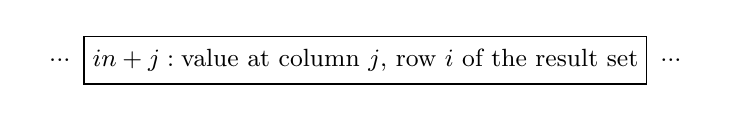
\begin{tikzpicture}
\small
\matrix[nodes={minimum size=6mm}] {
  \node {...};
 &\node[draw] {$in+j:\textrm{value at column $j$, row $i$ of the result set}$};
 &\node {...};\\
};
\end{tikzpicture}

where $i$, $j$ start from 0.\\
\textbf{Side Effects:} none.\\
\textbf{Throws:} {\Tt{}SQLException\nwendquote} if database failure is encountered.\\
\bottomrule
\end{tabular}
\nwenddocs{}\nwbegincode{3}\sublabel{NW1Dx1yV-3OEpPU-1}\nwmargintag{{\nwtagstyle{}\subpageref{NW1Dx1yV-3OEpPU-1}}}\moddef{Read: DBQuery(2)~{\nwtagstyle{}\subpageref{NW1Dx1yV-3OEpPU-1}}}\endmoddef\nwstartdeflinemarkup\nwusesondefline{\\{NW46kjAM-Oyob-1}}\nwenddeflinemarkup
int[] \nwlinkedidentc{DBQuery}{NW1Dx1yV-3OEpPU-1}(final String sql, final int ncols) throws SQLException \{
  int[] output = new int[] \{ \};
  try (\LA{}Open \code{}conn\edoc{}~{\nwtagstyle{}\subpageref{NW1ODIS0-JT1v9-1}}\RA{}) \{
    Statement stmt = conn.createStatement(
      ResultSet.TYPE_SCROLL_INSENSITIVE, ResultSet.CONCUR_READ_ONLY);
    ResultSet res = stmt.executeQuery(sql);
    if (res.last()) \{
      \LA{}Flatten results~{\nwtagstyle{}\subpageref{NW1Dx1yV-3qcw3I-1}}\RA{}
    \}
    conn.close();
  \} catch (SQLException e) \{
    throw e;
  \}
  return output;
\}
\nwindexdefn{\nwixident{DBQuery}}{DBQuery}{NW1Dx1yV-3OEpPU-1}\eatline
\nwused{\\{NW46kjAM-Oyob-1}}\nwidentdefs{\\{{\nwixident{DBQuery}}{DBQuery}}}\nwendcode{}\nwbegindocs{4}Special version for DesktopController
\nwenddocs{}\nwbegincode{5}\sublabel{NW1Dx1yV-1ag3qA-1}\nwmargintag{{\nwtagstyle{}\subpageref{NW1Dx1yV-1ag3qA-1}}}\moddef{Read: DBQueryQuick(3)~{\nwtagstyle{}\subpageref{NW1Dx1yV-1ag3qA-1}}}\endmoddef\nwstartdeflinemarkup\nwusesondefline{\\{NW46kjAM-Oyob-1}}\nwenddeflinemarkup
int[] \nwlinkedidentc{DBQueryQuick}{NW1Dx1yV-1ag3qA-1}(final String sql, int[] outcols, ArrayList<String> header) throws SQLException \{
  int[] output = new int[] \{ \};
  try (\LA{}Open \code{}conn\edoc{}~{\nwtagstyle{}\subpageref{NW1ODIS0-JT1v9-1}}\RA{}) \{
    Statement stmt = conn.createStatement(
      ResultSet.TYPE_SCROLL_INSENSITIVE, ResultSet.CONCUR_READ_ONLY);
    ResultSet res = stmt.executeQuery(sql);
    int ncols = res.getMetaData().getColumnCount();
    for (int i = 1; i <= ncols; i++) \{
      header.add(res.getMetaData().getColumnName(i));
    \}
    outcols[0] = ncols;
    if (res.last()) \{
      \LA{}Flatten results~{\nwtagstyle{}\subpageref{NW1Dx1yV-3qcw3I-1}}\RA{}
    \}
    conn.close();
  \} catch (SQLException e) \{
    throw e;
  \}
  return output;
\}
\nwindexdefn{\nwixident{DBQueryQuick}}{DBQueryQuick}{NW1Dx1yV-1ag3qA-1}\eatline
\nwused{\\{NW46kjAM-Oyob-1}}\nwidentdefs{\\{{\nwixident{DBQueryQuick}}{DBQueryQuick}}}\nwendcode{}\nwbegindocs{6}\begin{tabular}{p{\textwidth}}
\toprule
\rowcolor{TableTitle}
Method \textcolor{blue}{{\Tt{}\nwlinkedidentq{query}{NW1Dx1yV-47dtTX-1}\nwendquote}}(2) wraps {\Tt{}\nwlinkedidentq{DBQuery}{NW1Dx1yV-3OEpPU-1}\nwendquote}(2).\\
\bottomrule
\end{tabular}
\nwenddocs{}\nwbegincode{7}\sublabel{NW1Dx1yV-47dtTX-1}\nwmargintag{{\nwtagstyle{}\subpageref{NW1Dx1yV-47dtTX-1}}}\moddef{Read: query(2)~{\nwtagstyle{}\subpageref{NW1Dx1yV-47dtTX-1}}}\endmoddef\nwstartdeflinemarkup\nwusesondefline{\\{NW3hMOhb-2u8vSA-1}}\nwenddeflinemarkup
int[] \nwlinkedidentc{query}{NW1Dx1yV-47dtTX-1}(final String sql, final int ncols) throws SQLException \{
  int[] output = this.storage.\nwlinkedidentc{DBQuery}{NW1Dx1yV-3OEpPU-1}(sql, ncols);
  return output;
\}
\nwindexdefn{\nwixident{query}}{query}{NW1Dx1yV-47dtTX-1}\eatline
\nwused{\\{NW3hMOhb-2u8vSA-1}}\nwidentdefs{\\{{\nwixident{query}}{query}}}\nwidentuses{\\{{\nwixident{DBQuery}}{DBQuery}}}\nwindexuse{\nwixident{DBQuery}}{DBQuery}{NW1Dx1yV-47dtTX-1}\nwendcode{}\nwbegincode{8}\sublabel{NW1Dx1yV-5N7k3-1}\nwmargintag{{\nwtagstyle{}\subpageref{NW1Dx1yV-5N7k3-1}}}\moddef{Read: queryQuick(3)~{\nwtagstyle{}\subpageref{NW1Dx1yV-5N7k3-1}}}\endmoddef\nwstartdeflinemarkup\nwusesondefline{\\{NW3hMOhb-2u8vSA-1}}\nwenddeflinemarkup
int[] \nwlinkedidentc{queryQuick}{NW1Dx1yV-5N7k3-1}(final String sql, int[] outcols, ArrayList<String> header) throws SQLException \{
  long A0 = System.currentTimeMillis();
  int[] output = this.storage.\nwlinkedidentc{DBQueryQuick}{NW1Dx1yV-1ag3qA-1}(sql, outcols, header);
  this.dur_query = System.currentTimeMillis() - A0;
  return output;
\}
\nwindexdefn{\nwixident{queryQuick}}{queryQuick}{NW1Dx1yV-5N7k3-1}\eatline
\nwused{\\{NW3hMOhb-2u8vSA-1}}\nwidentdefs{\\{{\nwixident{queryQuick}}{queryQuick}}}\nwidentuses{\\{{\nwixident{DBQueryQuick}}{DBQueryQuick}}}\nwindexuse{\nwixident{DBQueryQuick}}{DBQueryQuick}{NW1Dx1yV-5N7k3-1}\nwendcode{}\nwbegindocs{9}\nwdocspar
\subsection{Methods: Read Road Network}

\subsubsection{\texttt{DBQueryMBR}(0)}
\begin{tabular}{p{\textwidth}}
\toprule
\rowcolor{TableTitle}
Method \textcolor{blue}{{\Tt{}\nwlinkedidentq{DBQueryMBR}{NW1Dx1yV-17SWaf-1}\nwendquote}}(0) returns the minimum-bounding
rectangle of the road network.
A {\Tt{}SQLException\nwendquote} is thrown in case of database failure.\\
\midrule
\textbf{Parameters:} none.\\
\textbf{Returns:} results of the query flattened into an integer array, or
{\Tt{}null\nwendquote} if no results.

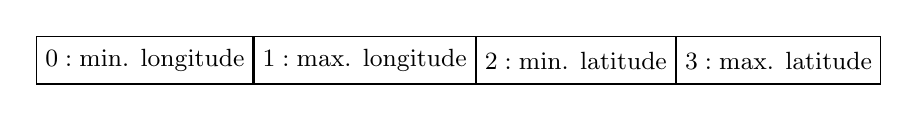
\begin{tikzpicture}
\small
\matrix[nodes={draw,minimum size=6mm}] {
  \node {$0:\textrm{min. longitude}$};
 &\node {$1:\textrm{max. longitude}$};
 &\node {$2:\textrm{min. latitude}$};
 &\node {$3:\textrm{max. latitude}$};\\
};
\end{tikzpicture}\\
\textbf{Side Effects:} none.\\
\textbf{Throws:} {\Tt{}SQLException\nwendquote} if database failure is encountered.\\
\bottomrule
\end{tabular}
\nwenddocs{}\nwbegincode{10}\sublabel{NW1Dx1yV-17SWaf-1}\nwmargintag{{\nwtagstyle{}\subpageref{NW1Dx1yV-17SWaf-1}}}\moddef{Read: DBQueryMBR(0)~{\nwtagstyle{}\subpageref{NW1Dx1yV-17SWaf-1}}}\endmoddef\nwstartdeflinemarkup\nwusesondefline{\\{NW46kjAM-Oyob-1}}\nwenddeflinemarkup
int[] \nwlinkedidentc{DBQueryMBR}{NW1Dx1yV-17SWaf-1}() throws SQLException \{
  try (\LA{}Open \code{}conn\edoc{}~{\nwtagstyle{}\subpageref{NW1ODIS0-JT1v9-1}}\RA{}) \{
    return this.\nwlinkedidentc{PSQuery}{NW1ODIS0-yHOIP-1}(conn, "\nwlinkedidentc{S64}{NW1ODIS0-zH56q-1}", 4);
  \} catch (SQLException e) \{
    throw e;
  \}
\}
\nwindexdefn{\nwixident{DBQueryMBR}}{DBQueryMBR}{NW1Dx1yV-17SWaf-1}\eatline
\nwused{\\{NW46kjAM-Oyob-1}}\nwidentdefs{\\{{\nwixident{DBQueryMBR}}{DBQueryMBR}}}\nwidentuses{\\{{\nwixident{PSQuery}}{PSQuery}}\\{{\nwixident{S64}}{S64}}}\nwindexuse{\nwixident{PSQuery}}{PSQuery}{NW1Dx1yV-17SWaf-1}\nwindexuse{\nwixident{S64}}{S64}{NW1Dx1yV-17SWaf-1}\nwendcode{}\nwbegindocs{11}\begin{tabular}{p{\textwidth}}
\toprule
\rowcolor{TableTitle}
Method \textcolor{blue}{{\Tt{}\nwlinkedidentq{queryMBR}{NW1Dx1yV-4JQRjd-1}\nwendquote}}(0) wraps {\Tt{}\nwlinkedidentq{DBQueryMBR}{NW1Dx1yV-17SWaf-1}\nwendquote}(0).\\
\bottomrule
\end{tabular}
\nwenddocs{}\nwbegincode{12}\sublabel{NW1Dx1yV-4JQRjd-1}\nwmargintag{{\nwtagstyle{}\subpageref{NW1Dx1yV-4JQRjd-1}}}\moddef{Read: queryMBR(0)~{\nwtagstyle{}\subpageref{NW1Dx1yV-4JQRjd-1}}}\endmoddef\nwstartdeflinemarkup\nwusesondefline{\\{NW3hMOhb-2u8vSA-1}}\nwenddeflinemarkup
int[] \nwlinkedidentc{queryMBR}{NW1Dx1yV-4JQRjd-1}() throws SQLException \{
  int[] output = this.storage.\nwlinkedidentc{DBQueryMBR}{NW1Dx1yV-17SWaf-1}();
  return output;
\}
\nwindexdefn{\nwixident{queryMBR}}{queryMBR}{NW1Dx1yV-4JQRjd-1}\eatline
\nwused{\\{NW3hMOhb-2u8vSA-1}}\nwidentdefs{\\{{\nwixident{queryMBR}}{queryMBR}}}\nwidentuses{\\{{\nwixident{DBQueryMBR}}{DBQueryMBR}}}\nwindexuse{\nwixident{DBQueryMBR}}{DBQueryMBR}{NW1Dx1yV-4JQRjd-1}\nwendcode{}\nwbegindocs{13}\nwdocspar
\subsubsection{\texttt{DBQueryVertex}(1)}
\begin{tabular}{p{\textwidth}}
\toprule
\rowcolor{TableTitle}
Method \textcolor{blue}{{\Tt{}\nwlinkedidentq{DBQueryVertex}{NW1Dx1yV-48j64d-1}\nwendquote}}(1) returns the longitude and
latitude coordinates of the given vertex. If the vertex does not exist,
a {\Tt{}\nwlinkedidentq{VertexNotFoundException}{NW1ODIS0-2ZrcAK-1}\nwendquote} is thrown.\\
\midrule
\textbf{Parameters:} \\
\begin{tabular}{lp{116mm}}
Integer {\Tt{}v\nwendquote} (param. 1):&vertex identifier.
\end{tabular}
\textbf{Returns:} results of the query flattened into an integer array, or
{\Tt{}null\nwendquote} if no results.

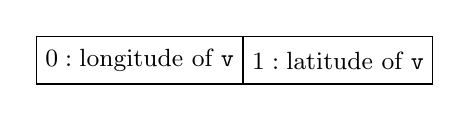
\begin{tikzpicture}
\small
\matrix[nodes={draw,minimum size=6mm}] {
  \node {$0:\textrm{longitude of }\texttt{v}$};
 &\node {$1:\textrm{latitude of }\texttt{v}$};\\
};
\end{tikzpicture}\\
\textbf{Side Effects:} none.\\
\textbf{Throws:} {\Tt{}\nwlinkedidentq{VertexNotFoundException}{NW1ODIS0-2ZrcAK-1}\nwendquote} if vertex does not exist\\
\bottomrule
\end{tabular}
\nwenddocs{}\nwbegincode{14}\sublabel{NW1Dx1yV-48j64d-1}\nwmargintag{{\nwtagstyle{}\subpageref{NW1Dx1yV-48j64d-1}}}\moddef{Read: DBQueryVertex(1)~{\nwtagstyle{}\subpageref{NW1Dx1yV-48j64d-1}}}\endmoddef\nwstartdeflinemarkup\nwusesondefline{\\{NW46kjAM-Oyob-1}\\{NW4SYVd2-3QhyAk-1}}\nwenddeflinemarkup
int[] \nwlinkedidentc{DBQueryVertex}{NW1Dx1yV-48j64d-1}(final int v) throws \nwlinkedidentc{VertexNotFoundException}{NW1ODIS0-2ZrcAK-1} \{
  if (!this.lu_vertices.containsKey(v)) \{
    throw new \nwlinkedidentc{VertexNotFoundException}{NW1ODIS0-2ZrcAK-1}("Vertex "+v+" not found.");
  \}
  int[] output = this.lu_vertices.get(v).clone();
  return new int[] \{ output[0], output[1], (int) Storage.CSHIFT \};
\}
\nwindexdefn{\nwixident{DBQueryVertex}}{DBQueryVertex}{NW1Dx1yV-48j64d-1}\eatline
\nwused{\\{NW46kjAM-Oyob-1}\\{NW4SYVd2-3QhyAk-1}}\nwidentdefs{\\{{\nwixident{DBQueryVertex}}{DBQueryVertex}}}\nwidentuses{\\{{\nwixident{VertexNotFoundException}}{VertexNotFoundException}}}\nwindexuse{\nwixident{VertexNotFoundException}}{VertexNotFoundException}{NW1Dx1yV-48j64d-1}\nwendcode{}\nwbegindocs{15}\begin{tabular}{p{\textwidth}}
\toprule
\rowcolor{TableTitle}
Method \textcolor{blue}{{\Tt{}\nwlinkedidentq{queryVertex}{NW1Dx1yV-oIN5n-1}\nwendquote}}(1) wraps {\Tt{}\nwlinkedidentq{DBQueryVertex}{NW1Dx1yV-48j64d-1}\nwendquote}(1).\\
\bottomrule
\end{tabular}
\nwenddocs{}\nwbegincode{16}\sublabel{NW1Dx1yV-oIN5n-1}\nwmargintag{{\nwtagstyle{}\subpageref{NW1Dx1yV-oIN5n-1}}}\moddef{Read: queryVertex(1)~{\nwtagstyle{}\subpageref{NW1Dx1yV-oIN5n-1}}}\endmoddef\nwstartdeflinemarkup\nwusesondefline{\\{NW3hMOhb-2u8vSA-1}\\{NW1y1NkR-2Rlctf-1}}\nwenddeflinemarkup
int[] \nwlinkedidentc{queryVertex}{NW1Dx1yV-oIN5n-1}(final int v) throws \nwlinkedidentc{VertexNotFoundException}{NW1ODIS0-2ZrcAK-1}, SQLException \{
  int[] output = this.storage.\nwlinkedidentc{DBQueryVertex}{NW1Dx1yV-48j64d-1}(v);
  return output;
\}
\nwindexdefn{\nwixident{queryVertex}}{queryVertex}{NW1Dx1yV-oIN5n-1}\eatline
\nwused{\\{NW3hMOhb-2u8vSA-1}\\{NW1y1NkR-2Rlctf-1}}\nwidentdefs{\\{{\nwixident{queryVertex}}{queryVertex}}}\nwidentuses{\\{{\nwixident{DBQueryVertex}}{DBQueryVertex}}\\{{\nwixident{VertexNotFoundException}}{VertexNotFoundException}}}\nwindexuse{\nwixident{DBQueryVertex}}{DBQueryVertex}{NW1Dx1yV-oIN5n-1}\nwindexuse{\nwixident{VertexNotFoundException}}{VertexNotFoundException}{NW1Dx1yV-oIN5n-1}\nwendcode{}\nwbegindocs{17}\nwdocspar
\subsubsection{\texttt{DBQueryVertices}(0)}
\begin{tabular}{p{\textwidth}}
\toprule
\rowcolor{TableTitle}
Method \textcolor{blue}{{\Tt{}\nwlinkedidentq{DBQueryVertices}{NW1Dx1yV-1imYqa-1}\nwendquote}}(0) returns all rows in Table V.
A {\Tt{}SQLException\nwendquote} is thrown in case of database failure.\\
\midrule
\textbf{Parameters:} none.\\
\textbf{Returns:} results of the query flattened into an integer array, or
{\Tt{}null\nwendquote} if no results.

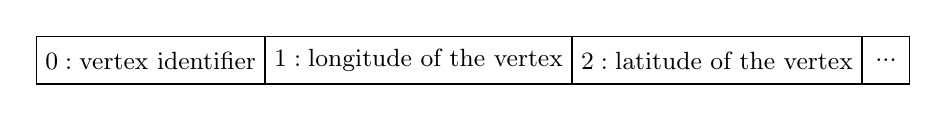
\begin{tikzpicture}
\small
\matrix[nodes={draw,minimum size=6mm}] {
  \node {$0:\textrm{vertex identifier}$};
 &\node {$1:\textrm{longitude of the vertex}$};
 &\node {$2:\textrm{latitude of the vertex}$};
 &\node {...};\\
};
\end{tikzpicture}\\
\textbf{Side Effects:} none.\\
\textbf{Throws:} {\Tt{}SQLException\nwendquote} if database failure is encountered.\\
\bottomrule
\end{tabular}
\nwenddocs{}\nwbegincode{18}\sublabel{NW1Dx1yV-1imYqa-1}\nwmargintag{{\nwtagstyle{}\subpageref{NW1Dx1yV-1imYqa-1}}}\moddef{Read: DBQueryVertices(0)~{\nwtagstyle{}\subpageref{NW1Dx1yV-1imYqa-1}}}\endmoddef\nwstartdeflinemarkup\nwusesondefline{\\{NW46kjAM-Oyob-1}}\nwenddeflinemarkup
int[] \nwlinkedidentc{DBQueryVertices}{NW1Dx1yV-1imYqa-1}() throws SQLException \{
  try (\LA{}Open \code{}conn\edoc{}~{\nwtagstyle{}\subpageref{NW1ODIS0-JT1v9-1}}\RA{}) \{
    return this.\nwlinkedidentc{PSQuery}{NW1ODIS0-yHOIP-1}(conn, "\nwlinkedidentc{S136}{NW1ODIS0-26ZLfn-1}", 3);
  \} catch (SQLException e) \{
    throw e;
  \}
\}
\nwindexdefn{\nwixident{DBQueryVertices}}{DBQueryVertices}{NW1Dx1yV-1imYqa-1}\eatline
\nwused{\\{NW46kjAM-Oyob-1}}\nwidentdefs{\\{{\nwixident{DBQueryVertices}}{DBQueryVertices}}}\nwidentuses{\\{{\nwixident{PSQuery}}{PSQuery}}\\{{\nwixident{S136}}{S136}}}\nwindexuse{\nwixident{PSQuery}}{PSQuery}{NW1Dx1yV-1imYqa-1}\nwindexuse{\nwixident{S136}}{S136}{NW1Dx1yV-1imYqa-1}\nwendcode{}\nwbegindocs{19}\begin{tabular}{p{\textwidth}}
\toprule
\rowcolor{TableTitle}
Method \textcolor{blue}{{\Tt{}\nwlinkedidentq{queryVertices}{NW1Dx1yV-435mrM-1}\nwendquote}}(2) wraps {\Tt{}\nwlinkedidentq{DBQueryVertices}{NW1Dx1yV-1imYqa-1}\nwendquote}(2).\\
\bottomrule
\end{tabular}
\nwenddocs{}\nwbegincode{20}\sublabel{NW1Dx1yV-435mrM-1}\nwmargintag{{\nwtagstyle{}\subpageref{NW1Dx1yV-435mrM-1}}}\moddef{Read: queryVertices(0)~{\nwtagstyle{}\subpageref{NW1Dx1yV-435mrM-1}}}\endmoddef\nwstartdeflinemarkup\nwusesondefline{\\{NW3hMOhb-2u8vSA-1}}\nwenddeflinemarkup
int[] \nwlinkedidentc{queryVertices}{NW1Dx1yV-435mrM-1}() throws SQLException \{
  int[] output = this.storage.\nwlinkedidentc{DBQueryVertices}{NW1Dx1yV-1imYqa-1}();
  return output;
\}
\nwindexdefn{\nwixident{queryVertices}}{queryVertices}{NW1Dx1yV-435mrM-1}\eatline
\nwused{\\{NW3hMOhb-2u8vSA-1}}\nwidentdefs{\\{{\nwixident{queryVertices}}{queryVertices}}}\nwidentuses{\\{{\nwixident{DBQueryVertices}}{DBQueryVertices}}}\nwindexuse{\nwixident{DBQueryVertices}}{DBQueryVertices}{NW1Dx1yV-435mrM-1}\nwendcode{}\nwbegindocs{21}\nwdocspar
\subsubsection{\texttt{DBQueryVerticesCount}(0)}
\begin{tabular}{p{\textwidth}}
\toprule
\rowcolor{TableTitle}
Method \textcolor{blue}{{\Tt{}\nwlinkedidentq{DBQueryVerticesCount}{NW1Dx1yV-1C883O-1}\nwendquote}}(0) returns the total number
of vertices in Table V.
A {\Tt{}SQLException\nwendquote} is thrown in case of database failure.\\
\midrule
\textbf{Parameters:} none.\\
\textbf{Returns:} results of the query flattened into an integer array, or
{\Tt{}null\nwendquote} if no results.

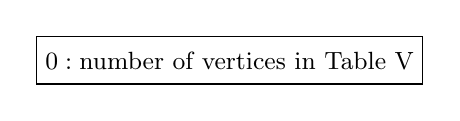
\begin{tikzpicture}
\small
\matrix[nodes={draw,minimum size=6mm}] {
  \node {$0:\textrm{number of vertices in Table V}$};\\
};
\end{tikzpicture}\\
\textbf{Side Effects:} none.\\
\textbf{Throws:} {\Tt{}SQLException\nwendquote} if database failure is encountered.\\
\bottomrule
\end{tabular}
\nwenddocs{}\nwbegincode{22}\sublabel{NW1Dx1yV-1C883O-1}\nwmargintag{{\nwtagstyle{}\subpageref{NW1Dx1yV-1C883O-1}}}\moddef{Read: DBQueryVerticesCount(0)~{\nwtagstyle{}\subpageref{NW1Dx1yV-1C883O-1}}}\endmoddef\nwstartdeflinemarkup\nwusesondefline{\\{NW46kjAM-Oyob-1}}\nwenddeflinemarkup
int[] \nwlinkedidentc{DBQueryVerticesCount}{NW1Dx1yV-1C883O-1}() throws SQLException \{
  try (\LA{}Open \code{}conn\edoc{}~{\nwtagstyle{}\subpageref{NW1ODIS0-JT1v9-1}}\RA{}) \{
    return this.\nwlinkedidentc{PSQuery}{NW1ODIS0-yHOIP-1}(conn, "\nwlinkedidentc{S62}{NW1ODIS0-25gPSO-1}", 1);
  \} catch (SQLException e) \{
    throw e;
  \}
\}
\nwindexdefn{\nwixident{DBQueryVerticesCount}}{DBQueryVerticesCount}{NW1Dx1yV-1C883O-1}\eatline
\nwused{\\{NW46kjAM-Oyob-1}}\nwidentdefs{\\{{\nwixident{DBQueryVerticesCount}}{DBQueryVerticesCount}}}\nwidentuses{\\{{\nwixident{PSQuery}}{PSQuery}}\\{{\nwixident{S62}}{S62}}}\nwindexuse{\nwixident{PSQuery}}{PSQuery}{NW1Dx1yV-1C883O-1}\nwindexuse{\nwixident{S62}}{S62}{NW1Dx1yV-1C883O-1}\nwendcode{}\nwbegindocs{23}\begin{tabular}{p{\textwidth}}
\toprule
\rowcolor{TableTitle}
Method \textcolor{blue}{{\Tt{}\nwlinkedidentq{queryVerticesCount}{NW1Dx1yV-EkhgX-1}\nwendquote}}(0) wraps {\Tt{}\nwlinkedidentq{DBQueryVerticesCount}{NW1Dx1yV-1C883O-1}\nwendquote}(0).\\
\bottomrule
\end{tabular}
\nwenddocs{}\nwbegincode{24}\sublabel{NW1Dx1yV-EkhgX-1}\nwmargintag{{\nwtagstyle{}\subpageref{NW1Dx1yV-EkhgX-1}}}\moddef{Read: queryVerticesCount(0)~{\nwtagstyle{}\subpageref{NW1Dx1yV-EkhgX-1}}}\endmoddef\nwstartdeflinemarkup\nwusesondefline{\\{NW3hMOhb-2u8vSA-1}}\nwenddeflinemarkup
int[] \nwlinkedidentc{queryVerticesCount}{NW1Dx1yV-EkhgX-1}() throws SQLException \{
  int[] output = this.storage.\nwlinkedidentc{DBQueryVerticesCount}{NW1Dx1yV-1C883O-1}();
  return output;
\}
\nwindexdefn{\nwixident{queryVerticesCount}}{queryVerticesCount}{NW1Dx1yV-EkhgX-1}\eatline
\nwused{\\{NW3hMOhb-2u8vSA-1}}\nwidentdefs{\\{{\nwixident{queryVerticesCount}}{queryVerticesCount}}}\nwidentuses{\\{{\nwixident{DBQueryVerticesCount}}{DBQueryVerticesCount}}}\nwindexuse{\nwixident{DBQueryVerticesCount}}{DBQueryVerticesCount}{NW1Dx1yV-EkhgX-1}\nwendcode{}\nwbegindocs{25}\nwdocspar
\subsubsection{\texttt{DBQueryEdge}(2)}
\begin{tabular}{p{\textwidth}}
\toprule
\rowcolor{TableTitle}
Method \textcolor{blue}{{\Tt{}\nwlinkedidentq{DBQueryEdge}{NW1Dx1yV-1eCWox-1}\nwendquote}}(2) returns the distance and
maximum free-flow speed along the given edge.
An {\Tt{}\nwlinkedidentq{EdgeNotFoundException}{NW1ODIS0-4YUrEC-1}\nwendquote} is thrown if the edge does not exist.\\
\midrule
\textbf{Parameters:} \\
\begin{tabular}{lp{116mm}}
Integer {\Tt{}v1\nwendquote} (param. 1):&source vertex identifier $v_1$\\
Integer {\Tt{}v2\nwendquote} (param. 2):&target vertex identifier $v_2$
\end{tabular}\\
\textbf{Returns:} results of the query flattened into an integer array, or
{\Tt{}null\nwendquote} if no results.

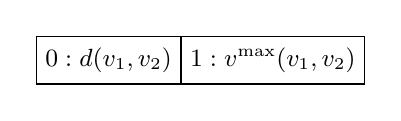
\begin{tikzpicture}
\small
\matrix[nodes={draw,minimum size=6mm}] {
  \node {$0:d(v_1,v_2)$}; & \node {$1:v^\textrm{max}(v_1,v_2)$}; \\
};
\end{tikzpicture}\\
\textbf{Side Effects:} none.\\
\textbf{Throws:} {\Tt{}\nwlinkedidentq{EdgeNotFoundException}{NW1ODIS0-4YUrEC-1}\nwendquote} if edge does not exit.\\
\bottomrule
\end{tabular}
\nwenddocs{}\nwbegincode{26}\sublabel{NW1Dx1yV-1eCWox-1}\nwmargintag{{\nwtagstyle{}\subpageref{NW1Dx1yV-1eCWox-1}}}\moddef{Read: DBQueryEdge(2)~{\nwtagstyle{}\subpageref{NW1Dx1yV-1eCWox-1}}}\endmoddef\nwstartdeflinemarkup\nwusesondefline{\\{NW46kjAM-Oyob-1}\\{NW4SYVd2-3QhyAk-1}}\nwenddeflinemarkup
int[] \nwlinkedidentc{DBQueryEdge}{NW1Dx1yV-1eCWox-1}(final int v1, final int v2) throws \nwlinkedidentc{EdgeNotFoundException}{NW1ODIS0-4YUrEC-1} \{
  if (v1 == v2) \{
    return new int[] \{ 0, -1 \};  // 0 distance, -1 speed
  \}
  if (!(this.lu_edges.containsKey(v1) && this.lu_edges.get(v1).containsKey(v2))) \{
    throw new \nwlinkedidentc{EdgeNotFoundException}{NW1ODIS0-4YUrEC-1}("Edge ("+v1+", "+v2+") not found.");
  \}
  return this.lu_edges.get(v1).get(v2).clone();
\}
\nwindexdefn{\nwixident{DBQueryEdge}}{DBQueryEdge}{NW1Dx1yV-1eCWox-1}\eatline
\nwused{\\{NW46kjAM-Oyob-1}\\{NW4SYVd2-3QhyAk-1}}\nwidentdefs{\\{{\nwixident{DBQueryEdge}}{DBQueryEdge}}}\nwidentuses{\\{{\nwixident{EdgeNotFoundException}}{EdgeNotFoundException}}}\nwindexuse{\nwixident{EdgeNotFoundException}}{EdgeNotFoundException}{NW1Dx1yV-1eCWox-1}\nwendcode{}\nwbegindocs{27}\begin{tabular}{p{\textwidth}}
\toprule
\rowcolor{TableTitle}
Method \textcolor{blue}{{\Tt{}\nwlinkedidentq{queryEdge}{NW1Dx1yV-1H3Dhp-1}\nwendquote}}(2) wraps {\Tt{}\nwlinkedidentq{DBQueryEdge}{NW1Dx1yV-1eCWox-1}\nwendquote}(2).\\
\bottomrule
\end{tabular}
\nwenddocs{}\nwbegincode{28}\sublabel{NW1Dx1yV-1H3Dhp-1}\nwmargintag{{\nwtagstyle{}\subpageref{NW1Dx1yV-1H3Dhp-1}}}\moddef{Read: queryEdge(2)~{\nwtagstyle{}\subpageref{NW1Dx1yV-1H3Dhp-1}}}\endmoddef\nwstartdeflinemarkup\nwusesondefline{\\{NW3hMOhb-2u8vSA-1}\\{NW1y1NkR-2Rlctf-1}}\nwenddeflinemarkup
int[] \nwlinkedidentc{queryEdge}{NW1Dx1yV-1H3Dhp-1}(final int v1, final int v2) throws \nwlinkedidentc{EdgeNotFoundException}{NW1ODIS0-4YUrEC-1}, SQLException \{
  int[] output = this.storage.\nwlinkedidentc{DBQueryEdge}{NW1Dx1yV-1eCWox-1}(v1, v2);
  return output;
\}
\nwindexdefn{\nwixident{queryEdge}}{queryEdge}{NW1Dx1yV-1H3Dhp-1}\eatline
\nwused{\\{NW3hMOhb-2u8vSA-1}\\{NW1y1NkR-2Rlctf-1}}\nwidentdefs{\\{{\nwixident{queryEdge}}{queryEdge}}}\nwidentuses{\\{{\nwixident{DBQueryEdge}}{DBQueryEdge}}\\{{\nwixident{EdgeNotFoundException}}{EdgeNotFoundException}}}\nwindexuse{\nwixident{DBQueryEdge}}{DBQueryEdge}{NW1Dx1yV-1H3Dhp-1}\nwindexuse{\nwixident{EdgeNotFoundException}}{EdgeNotFoundException}{NW1Dx1yV-1H3Dhp-1}\nwendcode{}\nwbegindocs{29}\nwdocspar
\subsubsection{\texttt{DBQueryEdges}(0)}
\begin{tabular}{p{\textwidth}}
\toprule
\rowcolor{TableTitle}
Method \textcolor{blue}{{\Tt{}\nwlinkedidentq{DBQueryEdges}{NW1Dx1yV-1uCRXX-1}\nwendquote}}(0) returns all rows in Table E.
A {\Tt{}SQLException\nwendquote} is thrown in case of database failure.\\
\midrule
\textbf{Parameters:} none.\\
\textbf{Returns:} results of the query flattened into an integer array, or
{\Tt{}null\nwendquote} if no results.

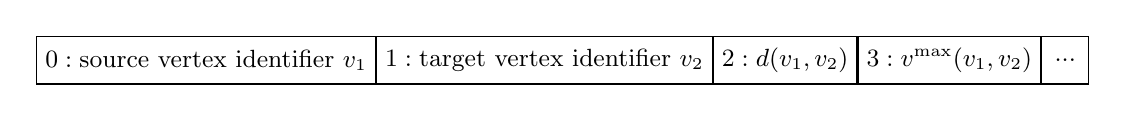
\begin{tikzpicture}
\small
\matrix[nodes={draw,minimum size=6mm}] {
  \node {$0:\textrm{source vertex identifier $v_1$}$};
 &\node {$1:\textrm{target vertex identifier $v_2$}$};
 &\node {$2:d(v_1,v_2)$};
 &\node {$3:v^\textrm{max}(v_1,v_2)$};
 &\node {...};\\
};
\end{tikzpicture}\\
\textbf{Side Effects:} none.\\
\textbf{Throws:} {\Tt{}SQLException\nwendquote} if database failure is encountered.\\
\bottomrule
\end{tabular}
\nwenddocs{}\nwbegincode{30}\sublabel{NW1Dx1yV-1uCRXX-1}\nwmargintag{{\nwtagstyle{}\subpageref{NW1Dx1yV-1uCRXX-1}}}\moddef{Read: DBQueryEdges(0)~{\nwtagstyle{}\subpageref{NW1Dx1yV-1uCRXX-1}}}\endmoddef\nwstartdeflinemarkup\nwusesondefline{\\{NW46kjAM-Oyob-1}}\nwenddeflinemarkup
int[] \nwlinkedidentc{DBQueryEdges}{NW1Dx1yV-1uCRXX-1}() throws SQLException \{
  try (\LA{}Open \code{}conn\edoc{}~{\nwtagstyle{}\subpageref{NW1ODIS0-JT1v9-1}}\RA{}) \{
    return this.\nwlinkedidentc{PSQuery}{NW1ODIS0-yHOIP-1}(conn, "\nwlinkedidentc{S137}{NW1ODIS0-2UPebD-1}", 4);
  \} catch (SQLException e) \{
    throw e;
  \}
\}
\nwindexdefn{\nwixident{DBQueryEdges}}{DBQueryEdges}{NW1Dx1yV-1uCRXX-1}\eatline
\nwused{\\{NW46kjAM-Oyob-1}}\nwidentdefs{\\{{\nwixident{DBQueryEdges}}{DBQueryEdges}}}\nwidentuses{\\{{\nwixident{PSQuery}}{PSQuery}}\\{{\nwixident{S137}}{S137}}}\nwindexuse{\nwixident{PSQuery}}{PSQuery}{NW1Dx1yV-1uCRXX-1}\nwindexuse{\nwixident{S137}}{S137}{NW1Dx1yV-1uCRXX-1}\nwendcode{}\nwbegindocs{31}\begin{tabular}{p{\textwidth}}
\toprule
\rowcolor{TableTitle}
Method \textcolor{blue}{{\Tt{}\nwlinkedidentq{queryEdges}{NW1Dx1yV-14B11a-1}\nwendquote}}(2) wraps {\Tt{}\nwlinkedidentq{DBQueryEdges}{NW1Dx1yV-1uCRXX-1}\nwendquote}(2).\\
\bottomrule
\end{tabular}
\nwenddocs{}\nwbegincode{32}\sublabel{NW1Dx1yV-14B11a-1}\nwmargintag{{\nwtagstyle{}\subpageref{NW1Dx1yV-14B11a-1}}}\moddef{Read: queryEdges(0)~{\nwtagstyle{}\subpageref{NW1Dx1yV-14B11a-1}}}\endmoddef\nwstartdeflinemarkup\nwusesondefline{\\{NW3hMOhb-2u8vSA-1}}\nwenddeflinemarkup
int[] \nwlinkedidentc{queryEdges}{NW1Dx1yV-14B11a-1}() throws SQLException \{
  int[] output = this.storage.\nwlinkedidentc{DBQueryEdges}{NW1Dx1yV-1uCRXX-1}();
  return output;
\}
\nwindexdefn{\nwixident{queryEdges}}{queryEdges}{NW1Dx1yV-14B11a-1}\eatline
\nwused{\\{NW3hMOhb-2u8vSA-1}}\nwidentdefs{\\{{\nwixident{queryEdges}}{queryEdges}}}\nwidentuses{\\{{\nwixident{DBQueryEdges}}{DBQueryEdges}}}\nwindexuse{\nwixident{DBQueryEdges}}{DBQueryEdges}{NW1Dx1yV-14B11a-1}\nwendcode{}\nwbegindocs{33}\nwdocspar
\subsubsection{\texttt{DBQueryEdgesCount}(0)}
\begin{tabular}{p{\textwidth}}
\toprule
\rowcolor{TableTitle}
Method \textcolor{blue}{{\Tt{}\nwlinkedidentq{DBQueryEdgesCount}{NW1Dx1yV-4bU7WY-1}\nwendquote}}(0) returns the total number
of vertices in Table V.
A {\Tt{}SQLException\nwendquote} is thrown in case of database failure.\\
\midrule
\textbf{Parameters:} none.\\
\textbf{Returns:} results of the query flattened into an integer array, or
{\Tt{}null\nwendquote} if no results.

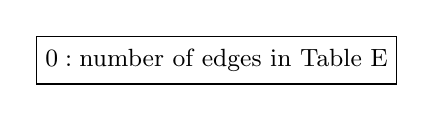
\begin{tikzpicture}
\small
\matrix[nodes={draw,minimum size=6mm}] {
  \node {$0:\textrm{number of edges in Table E}$};\\
};
\end{tikzpicture}\\
\textbf{Side Effects:} none.\\
\textbf{Throws:} {\Tt{}SQLException\nwendquote} if database failure is encountered.\\
\bottomrule
\end{tabular}
\nwenddocs{}\nwbegincode{34}\sublabel{NW1Dx1yV-4bU7WY-1}\nwmargintag{{\nwtagstyle{}\subpageref{NW1Dx1yV-4bU7WY-1}}}\moddef{Read: DBQueryEdgesCount(0)~{\nwtagstyle{}\subpageref{NW1Dx1yV-4bU7WY-1}}}\endmoddef\nwstartdeflinemarkup\nwusesondefline{\\{NW46kjAM-Oyob-1}}\nwenddeflinemarkup
int[] \nwlinkedidentc{DBQueryEdgesCount}{NW1Dx1yV-4bU7WY-1}() throws SQLException \{
  try (\LA{}Open \code{}conn\edoc{}~{\nwtagstyle{}\subpageref{NW1ODIS0-JT1v9-1}}\RA{}) \{
    return this.\nwlinkedidentc{PSQuery}{NW1ODIS0-yHOIP-1}(conn, "\nwlinkedidentc{S63}{NW1ODIS0-2TWiNo-1}", 1);
  \} catch (SQLException e) \{
    throw e;
  \}
\}
\nwindexdefn{\nwixident{DBQueryEdgesCount}}{DBQueryEdgesCount}{NW1Dx1yV-4bU7WY-1}\eatline
\nwused{\\{NW46kjAM-Oyob-1}}\nwidentdefs{\\{{\nwixident{DBQueryEdgesCount}}{DBQueryEdgesCount}}}\nwidentuses{\\{{\nwixident{PSQuery}}{PSQuery}}\\{{\nwixident{S63}}{S63}}}\nwindexuse{\nwixident{PSQuery}}{PSQuery}{NW1Dx1yV-4bU7WY-1}\nwindexuse{\nwixident{S63}}{S63}{NW1Dx1yV-4bU7WY-1}\nwendcode{}\nwbegindocs{35}\begin{tabular}{p{\textwidth}}
\toprule
\rowcolor{TableTitle}
Method \textcolor{blue}{{\Tt{}\nwlinkedidentq{queryEdgesCount}{NW1Dx1yV-3fg08d-1}\nwendquote}}(0) wraps {\Tt{}\nwlinkedidentq{DBQueryEdgesCount}{NW1Dx1yV-4bU7WY-1}\nwendquote}(0).\\
\bottomrule
\end{tabular}
\nwenddocs{}\nwbegincode{36}\sublabel{NW1Dx1yV-3fg08d-1}\nwmargintag{{\nwtagstyle{}\subpageref{NW1Dx1yV-3fg08d-1}}}\moddef{Read: queryEdgesCount(0)~{\nwtagstyle{}\subpageref{NW1Dx1yV-3fg08d-1}}}\endmoddef\nwstartdeflinemarkup\nwusesondefline{\\{NW3hMOhb-2u8vSA-1}}\nwenddeflinemarkup
int[] \nwlinkedidentc{queryEdgesCount}{NW1Dx1yV-3fg08d-1}() throws SQLException \{
  int[] output = this.storage.\nwlinkedidentc{DBQueryEdgesCount}{NW1Dx1yV-4bU7WY-1}();
  return output;
\}
\nwindexdefn{\nwixident{queryEdgesCount}}{queryEdgesCount}{NW1Dx1yV-3fg08d-1}\eatline
\nwused{\\{NW3hMOhb-2u8vSA-1}}\nwidentdefs{\\{{\nwixident{queryEdgesCount}}{queryEdgesCount}}}\nwidentuses{\\{{\nwixident{DBQueryEdgesCount}}{DBQueryEdgesCount}}}\nwindexuse{\nwixident{DBQueryEdgesCount}}{DBQueryEdgesCount}{NW1Dx1yV-3fg08d-1}\nwendcode{}\nwbegindocs{37}\nwdocspar
\subsubsection{\texttt{DBQueryEdgeStatistics}(0)}
\begin{tabular}{p{\textwidth}}
\toprule
\rowcolor{TableTitle}
Method \textcolor{blue}{{\Tt{}\nwlinkedidentq{DBQueryEdgeStatistics}{NW1Dx1yV-3w6nA9-1}\nwendquote}}(0) returns some edge statistics.
A {\Tt{}SQLException\nwendquote} is thrown in case of database failure.\\
\midrule
\textbf{Parameters:} none.\\
\textbf{Returns:} results of the query flattened into an integer array, or
{\Tt{}null\nwendquote} if no results.

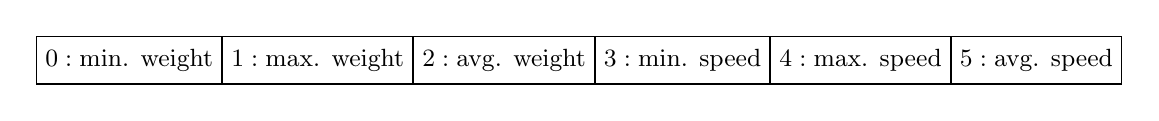
\begin{tikzpicture}
\small
\matrix[nodes={draw,minimum size=6mm}] {
  \node {$0:\textrm{min. weight}$};
 &\node {$1:\textrm{max. weight}$};
 &\node {$2:\textrm{avg. weight}$};
 &\node {$3:\textrm{min. speed}$};
 &\node {$4:\textrm{max. speed}$};
 &\node {$5:\textrm{avg. speed}$};\\
};
\end{tikzpicture}\\
\textbf{Side Effects:} none.\\
\textbf{Throws:} {\Tt{}SQLException\nwendquote} if database failure is encountered.\\
\bottomrule
\end{tabular}
\nwenddocs{}\nwbegincode{38}\sublabel{NW1Dx1yV-3w6nA9-1}\nwmargintag{{\nwtagstyle{}\subpageref{NW1Dx1yV-3w6nA9-1}}}\moddef{Read: DBQueryEdgeStatistics(0)~{\nwtagstyle{}\subpageref{NW1Dx1yV-3w6nA9-1}}}\endmoddef\nwstartdeflinemarkup\nwusesondefline{\\{NW46kjAM-Oyob-1}}\nwenddeflinemarkup
int[] \nwlinkedidentc{DBQueryEdgeStatistics}{NW1Dx1yV-3w6nA9-1}() throws SQLException \{
  try (\LA{}Open \code{}conn\edoc{}~{\nwtagstyle{}\subpageref{NW1ODIS0-JT1v9-1}}\RA{}) \{
    return this.\nwlinkedidentc{PSQuery}{NW1ODIS0-yHOIP-1}(conn, "\nwlinkedidentc{S65}{NW1ODIS0-3X63Qi-1}", 6);
  \} catch (SQLException e) \{
    throw e;
  \}
\}
\nwindexdefn{\nwixident{DBQueryEdgeStatistics}}{DBQueryEdgeStatistics}{NW1Dx1yV-3w6nA9-1}\eatline
\nwused{\\{NW46kjAM-Oyob-1}}\nwidentdefs{\\{{\nwixident{DBQueryEdgeStatistics}}{DBQueryEdgeStatistics}}}\nwidentuses{\\{{\nwixident{PSQuery}}{PSQuery}}\\{{\nwixident{S65}}{S65}}}\nwindexuse{\nwixident{PSQuery}}{PSQuery}{NW1Dx1yV-3w6nA9-1}\nwindexuse{\nwixident{S65}}{S65}{NW1Dx1yV-3w6nA9-1}\nwendcode{}\nwbegindocs{39}\begin{tabular}{p{\textwidth}}
\toprule
\rowcolor{TableTitle}
Method \textcolor{blue}{{\Tt{}\nwlinkedidentq{queryEdgeStatistics}{NW1Dx1yV-1SAYMv-1}\nwendquote}}(0) wraps {\Tt{}\nwlinkedidentq{DBQueryEdgeStatistics}{NW1Dx1yV-3w6nA9-1}\nwendquote}(0).\\
\bottomrule
\end{tabular}
\nwenddocs{}\nwbegincode{40}\sublabel{NW1Dx1yV-1SAYMv-1}\nwmargintag{{\nwtagstyle{}\subpageref{NW1Dx1yV-1SAYMv-1}}}\moddef{Read: queryEdgeStatistics(0)~{\nwtagstyle{}\subpageref{NW1Dx1yV-1SAYMv-1}}}\endmoddef\nwstartdeflinemarkup\nwusesondefline{\\{NW3hMOhb-2u8vSA-1}}\nwenddeflinemarkup
int[] \nwlinkedidentc{queryEdgeStatistics}{NW1Dx1yV-1SAYMv-1}() throws SQLException \{
  int[] output = storage.\nwlinkedidentc{DBQueryEdgeStatistics}{NW1Dx1yV-3w6nA9-1}();
  return output;
\}
\nwindexdefn{\nwixident{queryEdgeStatistics}}{queryEdgeStatistics}{NW1Dx1yV-1SAYMv-1}\eatline
\nwused{\\{NW3hMOhb-2u8vSA-1}}\nwidentdefs{\\{{\nwixident{queryEdgeStatistics}}{queryEdgeStatistics}}}\nwidentuses{\\{{\nwixident{DBQueryEdgeStatistics}}{DBQueryEdgeStatistics}}}\nwindexuse{\nwixident{DBQueryEdgeStatistics}}{DBQueryEdgeStatistics}{NW1Dx1yV-1SAYMv-1}\nwendcode{}\nwbegindocs{41}\nwdocspar
\subsection{Methods: Read User Properties}

\subsubsection{\texttt{DBQueryUser}(1)}
\begin{tabular}{p{\textwidth}}
\toprule
\rowcolor{TableTitle}
Method \textcolor{blue}{{\Tt{}\nwlinkedidentq{DBQueryUser}{NW1Dx1yV-8IJdE-1}\nwendquote}}(0) returns the properties of the
given user.
A {\Tt{}\nwlinkedidentq{UserNotFoundException}{NW1ODIS0-15irq2-1}\nwendquote} is thrown if the user does not exist.\\
\midrule
\textbf{Parameters:} \\
\begin{tabular}{lp{116mm}}
Integer {\Tt{}uid\nwendquote} (param. 1):&user identifier for user $u$
\end{tabular}
\textbf{Returns:} results of the query flattened into an integer array, or
{\Tt{}null\nwendquote} if no results.

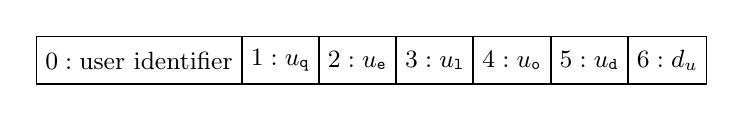
\begin{tikzpicture}
\small
\matrix[nodes={draw,minimum size=6mm}] {
  \node {$0:\textrm{user identifier}$};
 &\node {$1:u_\texttt{q}$};
 &\node {$2:u_\texttt{e}$};
 &\node {$3:u_\texttt{l}$};
 &\node {$4:u_\texttt{o}$};
 &\node {$5:u_\texttt{d}$};
 &\node {$6:d_u$};\\
};
\end{tikzpicture}\\
\textbf{Side Effects:} none.\\
\textbf{Throws:} {\Tt{}\nwlinkedidentq{UserNotFoundException}{NW1ODIS0-15irq2-1}\nwendquote} if user does not exist.\\
\bottomrule
\end{tabular}
\nwenddocs{}\nwbegincode{42}\sublabel{NW1Dx1yV-8IJdE-1}\nwmargintag{{\nwtagstyle{}\subpageref{NW1Dx1yV-8IJdE-1}}}\moddef{Read: DBQueryUser(1)~{\nwtagstyle{}\subpageref{NW1Dx1yV-8IJdE-1}}}\endmoddef\nwstartdeflinemarkup\nwusesondefline{\\{NW46kjAM-Oyob-1}}\nwenddeflinemarkup
int[] \nwlinkedidentc{DBQueryUser}{NW1Dx1yV-8IJdE-1}(final int uid)
throws \nwlinkedidentc{UserNotFoundException}{NW1ODIS0-15irq2-1} \{
  if (!this.lu_users.containsKey(uid)) \{
    throw new \nwlinkedidentc{UserNotFoundException}{NW1ODIS0-15irq2-1}("User "+uid+" not found.");
  \}
  return this.lu_users.get(uid).clone();
\}
\nwindexdefn{\nwixident{DBQueryUser}}{DBQueryUser}{NW1Dx1yV-8IJdE-1}\eatline
\nwused{\\{NW46kjAM-Oyob-1}}\nwidentdefs{\\{{\nwixident{DBQueryUser}}{DBQueryUser}}}\nwidentuses{\\{{\nwixident{UserNotFoundException}}{UserNotFoundException}}}\nwindexuse{\nwixident{UserNotFoundException}}{UserNotFoundException}{NW1Dx1yV-8IJdE-1}\nwendcode{}\nwbegindocs{43}\begin{tabular}{p{\textwidth}}
\toprule
\rowcolor{TableTitle}
Method \textcolor{blue}{{\Tt{}\nwlinkedidentq{queryUser}{NW1Dx1yV-SBVOE-1}\nwendquote}}(1) wraps {\Tt{}\nwlinkedidentq{DBQueryUser}{NW1Dx1yV-8IJdE-1}\nwendquote}(1).\\
\bottomrule
\end{tabular}
\nwenddocs{}\nwbegincode{44}\sublabel{NW1Dx1yV-SBVOE-1}\nwmargintag{{\nwtagstyle{}\subpageref{NW1Dx1yV-SBVOE-1}}}\moddef{Read: queryUser(1)~{\nwtagstyle{}\subpageref{NW1Dx1yV-SBVOE-1}}}\endmoddef\nwstartdeflinemarkup\nwusesondefline{\\{NW3hMOhb-2u8vSA-1}\\{NW1y1NkR-2Rlctf-1}}\nwenddeflinemarkup
int[] \nwlinkedidentc{queryUser}{NW1Dx1yV-SBVOE-1}(final int rid) throws \nwlinkedidentc{UserNotFoundException}{NW1ODIS0-15irq2-1}, SQLException \{
  int[] output = storage.\nwlinkedidentc{DBQueryUser}{NW1Dx1yV-8IJdE-1}(rid);
  return output;
\}
\nwindexdefn{\nwixident{queryUser}}{queryUser}{NW1Dx1yV-SBVOE-1}\eatline
\nwused{\\{NW3hMOhb-2u8vSA-1}\\{NW1y1NkR-2Rlctf-1}}\nwidentdefs{\\{{\nwixident{queryUser}}{queryUser}}}\nwidentuses{\\{{\nwixident{DBQueryUser}}{DBQueryUser}}\\{{\nwixident{UserNotFoundException}}{UserNotFoundException}}}\nwindexuse{\nwixident{DBQueryUser}}{DBQueryUser}{NW1Dx1yV-SBVOE-1}\nwindexuse{\nwixident{UserNotFoundException}}{UserNotFoundException}{NW1Dx1yV-SBVOE-1}\nwendcode{}\nwbegindocs{45}\nwdocspar
\subsubsection{\texttt{DBQueryUsers}(0)}
\begin{tabular}{p{\textwidth}}
\toprule
\rowcolor{TableTitle}
Method \textcolor{blue}{{\Tt{}\nwlinkedidentq{DBQueryUsers}{NW1Dx1yV-4dNZxZ-1}\nwendquote}}(0) returns all rows in view {\Tt{}r{\_}user\nwendquote}.
A {\Tt{}SQLException\nwendquote} is thrown in case of database failure.\\
\midrule
\textbf{Parameters:} none.\\
\textbf{Returns:} results of the query flattened into an integer array, or
{\Tt{}null\nwendquote} if no results.

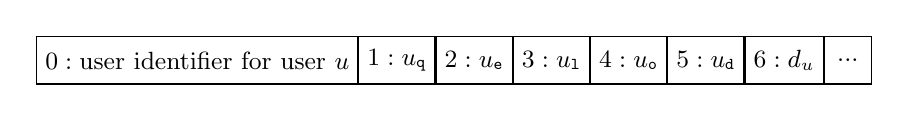
\begin{tikzpicture}
\small
\matrix[nodes={draw,minimum size=6mm}] {
  \node {$0:\textrm{user identifier for user $u$}$};
 &\node {$1:u_\texttt{q}$};
 &\node {$2:u_\texttt{e}$};
 &\node {$3:u_\texttt{l}$};
 &\node {$4:u_\texttt{o}$};
 &\node {$5:u_\texttt{d}$};
 &\node {$6:d_u$};
 &\node {...};\\
};
\end{tikzpicture}\\
\textbf{Side Effects:} none.\\
\textbf{Throws:} {\Tt{}SQLException\nwendquote} if database failure is encountered.\\
\bottomrule
\end{tabular}
\nwenddocs{}\nwbegincode{46}\sublabel{NW1Dx1yV-4dNZxZ-1}\nwmargintag{{\nwtagstyle{}\subpageref{NW1Dx1yV-4dNZxZ-1}}}\moddef{Read: DBQueryUsers(0)~{\nwtagstyle{}\subpageref{NW1Dx1yV-4dNZxZ-1}}}\endmoddef\nwstartdeflinemarkup\nwusesondefline{\\{NW46kjAM-Oyob-1}}\nwenddeflinemarkup
int[] \nwlinkedidentc{DBQueryUsers}{NW1Dx1yV-4dNZxZ-1}() throws SQLException \{
  try (\LA{}Open \code{}conn\edoc{}~{\nwtagstyle{}\subpageref{NW1ODIS0-JT1v9-1}}\RA{}) \{
    return this.\nwlinkedidentc{PSQuery}{NW1ODIS0-yHOIP-1}(conn, "\nwlinkedidentc{S141}{NW1ODIS0-3WcmPz-1}", 7);
  \} catch (SQLException e) \{
    throw e;
  \}
\}
\nwindexdefn{\nwixident{DBQueryUsers}}{DBQueryUsers}{NW1Dx1yV-4dNZxZ-1}\eatline
\nwused{\\{NW46kjAM-Oyob-1}}\nwidentdefs{\\{{\nwixident{DBQueryUsers}}{DBQueryUsers}}}\nwidentuses{\\{{\nwixident{PSQuery}}{PSQuery}}\\{{\nwixident{S141}}{S141}}}\nwindexuse{\nwixident{PSQuery}}{PSQuery}{NW1Dx1yV-4dNZxZ-1}\nwindexuse{\nwixident{S141}}{S141}{NW1Dx1yV-4dNZxZ-1}\nwendcode{}\nwbegindocs{47}\nwdocspar
\subsubsection{\texttt{DBQueryRequestStatus}(2)}
\begin{tabular}{p{\textwidth}}
\toprule
\rowcolor{TableTitle}
Method \textcolor{blue}{{\Tt{}\nwlinkedidentq{DBQueryRequestStatus}{NW1Dx1yV-2bbv1T-1}\nwendquote}}(0) returns the status of
the given request at the given time (Eq.~\ref{eq:status}).
A {\Tt{}\nwlinkedidentq{UserNotFoundException}{NW1ODIS0-15irq2-1}\nwendquote} is thrown if the user does not exist.
A {\Tt{}SQLException\nwendquote} is thrown in case of database failure.\\
\midrule
\textbf{Parameters:} \\
\begin{tabular}{lp{116mm}}
Integer {\Tt{}rid\nwendquote} (param. 1):&user identifier for request $r$\\
Integer {\Tt{}t\nwendquote} (param. 2):&a time
\end{tabular}\\
\textbf{Returns:} results of the query flattened into an integer array, or
{\Tt{}null\nwendquote} if no results.

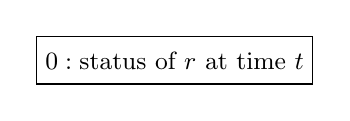
\begin{tikzpicture}
\small
\matrix[nodes={draw,minimum size=6mm}] {
  \node {$0:\textrm{status of $r$ at time $t$}$};\\
};
\end{tikzpicture}\\
\textbf{Side Effects:} none.\\
\textbf{Throws:} {\Tt{}\nwlinkedidentq{UserNotFoundException}{NW1ODIS0-15irq2-1}\nwendquote} if user does not exist, or
{\Tt{}SQLException\nwendquote} if database failure is encountered.\\
\bottomrule
\end{tabular}
\nwenddocs{}\nwbegincode{48}\sublabel{NW1Dx1yV-2bbv1T-1}\nwmargintag{{\nwtagstyle{}\subpageref{NW1Dx1yV-2bbv1T-1}}}\moddef{Read: DBQueryRequestStatus(2)~{\nwtagstyle{}\subpageref{NW1Dx1yV-2bbv1T-1}}}\endmoddef\nwstartdeflinemarkup\nwusesondefline{\\{NW46kjAM-Oyob-1}}\nwenddeflinemarkup
int[] \nwlinkedidentc{DBQueryRequestStatus}{NW1Dx1yV-2bbv1T-1}(final int rid, final int t)
throws \nwlinkedidentc{UserNotFoundException}{NW1ODIS0-15irq2-1}, SQLException \{
  if (!this.lu_users.containsKey(rid)) \{
    throw new \nwlinkedidentc{UserNotFoundException}{NW1ODIS0-15irq2-1}("User "+rid+" not found.");
  \}
  try (\LA{}Open \code{}conn\edoc{}~{\nwtagstyle{}\subpageref{NW1ODIS0-JT1v9-1}}\RA{}) \{
    return this.\nwlinkedidentc{PSQuery}{NW1ODIS0-yHOIP-1}(conn, "\nwlinkedidentc{S133}{NW1ODIS0-3Q2E0J-1}", 1, rid, t);
  \} catch (SQLException e) \{
    throw e;
  \}
\}
\nwindexdefn{\nwixident{DBQueryRequestStatus}}{DBQueryRequestStatus}{NW1Dx1yV-2bbv1T-1}\eatline
\nwused{\\{NW46kjAM-Oyob-1}}\nwidentdefs{\\{{\nwixident{DBQueryRequestStatus}}{DBQueryRequestStatus}}}\nwidentuses{\\{{\nwixident{PSQuery}}{PSQuery}}\\{{\nwixident{S133}}{S133}}\\{{\nwixident{UserNotFoundException}}{UserNotFoundException}}}\nwindexuse{\nwixident{PSQuery}}{PSQuery}{NW1Dx1yV-2bbv1T-1}\nwindexuse{\nwixident{S133}}{S133}{NW1Dx1yV-2bbv1T-1}\nwindexuse{\nwixident{UserNotFoundException}}{UserNotFoundException}{NW1Dx1yV-2bbv1T-1}\nwendcode{}\nwbegindocs{49}\nwdocspar
\subsubsection{\texttt{DBQueryRequestIsAssigned}(2)}
TODO. This is really bad. If param 2 is false, the return is blank or the sid
of the server assigned to request param 1. But if param 2 is true, the return
is either blank or 1; no sid.
\nwenddocs{}\nwbegincode{50}\sublabel{NW1Dx1yV-1Ypj7S-1}\nwmargintag{{\nwtagstyle{}\subpageref{NW1Dx1yV-1Ypj7S-1}}}\moddef{Read: DBQueryRequestIsAssigned(2)~{\nwtagstyle{}\subpageref{NW1Dx1yV-1Ypj7S-1}}}\endmoddef\nwstartdeflinemarkup\nwusesondefline{\\{NW46kjAM-Oyob-1}}\nwenddeflinemarkup
int[] \nwlinkedidentc{DBQueryRequestIsAssigned}{NW1Dx1yV-1Ypj7S-1}(final int rid, boolean flag_usecache) throws SQLException \{
  if (flag_usecache) \{
    return this.lu_rstatus.get(rid) ? new int[] \{ 1 \} : new int[] \{ \};
  \} else \{
    try (\LA{}Open \code{}conn\edoc{}~{\nwtagstyle{}\subpageref{NW1ODIS0-JT1v9-1}}\RA{}) \{
      return this.\nwlinkedidentc{PSQuery}{NW1ODIS0-yHOIP-1}(conn, "\nwlinkedidentc{S148}{NW1ODIS0-n1SCR-1}", 1, rid);
    \} catch (SQLException e) \{
      throw e;
    \}
  \}
\}
\nwindexdefn{\nwixident{DBQueryRequestIsAssigned}}{DBQueryRequestIsAssigned}{NW1Dx1yV-1Ypj7S-1}\eatline
\nwused{\\{NW46kjAM-Oyob-1}}\nwidentdefs{\\{{\nwixident{DBQueryRequestIsAssigned}}{DBQueryRequestIsAssigned}}}\nwidentuses{\\{{\nwixident{PSQuery}}{PSQuery}}\\{{\nwixident{S148}}{S148}}}\nwindexuse{\nwixident{PSQuery}}{PSQuery}{NW1Dx1yV-1Ypj7S-1}\nwindexuse{\nwixident{S148}}{S148}{NW1Dx1yV-1Ypj7S-1}\nwendcode{}\nwbegindocs{51}\nwdocspar
\subsubsection{\texttt{DBQueryRequestDistanceDetour}(2)}
\begin{tabular}{p{\textwidth}}
\toprule
\rowcolor{TableTitle}
Method \textcolor{blue}{{\Tt{}\nwlinkedidentq{DBQueryRequestDistanceDetour}{NW1Dx1yV-3KL3Uc-1}\nwendquote}}(2) returns the
detour distance $D^\textrm{detour}(\mathcal{X},r)$
(Eq.~\ref{eq:detour-distance}) of the given request.
A {\Tt{}SQLException\nwendquote} is thrown in case of database failure.\\
\midrule
\textbf{Parameters:}\\
\begin{tabular}{lp{116mm}}
Integer {\Tt{}rid\nwendquote} (param. 1):&request identifier.
\end{tabular}\\
\textbf{Returns:} results of the query flattened into an integer array,
or {\Tt{}null\nwendquote} if no results.

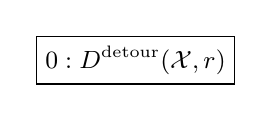
\begin{tikzpicture}
\small
\matrix[nodes={minimum size=6mm}] {
  \node[draw] {$0:D^\textrm{detour}(\mathcal{X},r)$};\\
};
\end{tikzpicture}

where $r$ is the request identified by {\Tt{}rid\nwendquote} (param. 1).\\
\textbf{Side Effects:} none.\\
\textbf{Throws:} {\Tt{}SQLException\nwendquote} if database failure is encountered.\\
\bottomrule
\end{tabular}
\nwenddocs{}\nwbegincode{52}\sublabel{NW1Dx1yV-3KL3Uc-1}\nwmargintag{{\nwtagstyle{}\subpageref{NW1Dx1yV-3KL3Uc-1}}}\moddef{Read: DBQueryRequestDistanceDetour(2)~{\nwtagstyle{}\subpageref{NW1Dx1yV-3KL3Uc-1}}}\endmoddef\nwstartdeflinemarkup\nwusesondefline{\\{NW46kjAM-Oyob-1}}\nwenddeflinemarkup
int[] \nwlinkedidentc{DBQueryRequestDistanceDetour}{NW1Dx1yV-3KL3Uc-1}(final int rid, boolean flag_usecache) throws SQLException \{
  if (flag_usecache) \{
    return new int[] \{ this.distance_requests_transit.containsKey(rid)
      ? this.distance_requests_transit.get(rid) - this.lu_users.get(rid)[6]
      : 0 \};
  \} else \{
    try (\LA{}Open \code{}conn\edoc{}~{\nwtagstyle{}\subpageref{NW1ODIS0-JT1v9-1}}\RA{}) \{
      return \nwlinkedidentc{PSQuery}{NW1ODIS0-yHOIP-1}(conn, "\nwlinkedidentc{S112}{NW1ODIS0-1SZQ6N-1}", 1, rid);
    \} catch (SQLException e) \{
      throw e;
    \}
  \}
\}
\nwindexdefn{\nwixident{DBQueryRequestDistanceDetour}}{DBQueryRequestDistanceDetour}{NW1Dx1yV-3KL3Uc-1}\eatline
\nwused{\\{NW46kjAM-Oyob-1}}\nwidentdefs{\\{{\nwixident{DBQueryRequestDistanceDetour}}{DBQueryRequestDistanceDetour}}}\nwidentuses{\\{{\nwixident{PSQuery}}{PSQuery}}\\{{\nwixident{S112}}{S112}}}\nwindexuse{\nwixident{PSQuery}}{PSQuery}{NW1Dx1yV-3KL3Uc-1}\nwindexuse{\nwixident{S112}}{S112}{NW1Dx1yV-3KL3Uc-1}\nwendcode{}\nwbegindocs{53}\nwdocspar
\subsubsection{\texttt{DBQueryRequestDistanceTransit}(2)}
\begin{tabular}{p{\textwidth}}
\toprule
\rowcolor{TableTitle}
Method \textcolor{blue}{{\Tt{}\nwlinkedidentq{DBQueryRequestDistanceTransit}{NW1Dx1yV-48YvP8-1}\nwendquote}}(2) returns the
transit distance $D^\textrm{transit}(\mathcal{X},r)$
(Eq.~\ref{eq:transit-distance}) of the given request.
A {\Tt{}SQLException\nwendquote} is thrown in case of database failure.\\
\midrule
\textbf{Parameters:}\\
\begin{tabular}{lp{116mm}}
Integer {\Tt{}rid\nwendquote} (param. 1):&request identifier.
\end{tabular}\\
\textbf{Returns:} results of the query flattened into an integer array,
or {\Tt{}null\nwendquote} if no results.

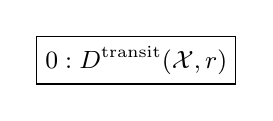
\begin{tikzpicture}
\small
\matrix[nodes={minimum size=6mm}] {
  \node[draw] {$0:D^\textrm{transit}(\mathcal{X},r)$};\\
};
\end{tikzpicture}

where $r$ is the request identified by {\Tt{}rid\nwendquote} (param. 1).\\
\textbf{Side Effects:} none.\\
\textbf{Throws:} {\Tt{}SQLException\nwendquote} if database failure is encountered.\\
\bottomrule
\end{tabular}
\nwenddocs{}\nwbegincode{54}\sublabel{NW1Dx1yV-48YvP8-1}\nwmargintag{{\nwtagstyle{}\subpageref{NW1Dx1yV-48YvP8-1}}}\moddef{Read: DBQueryRequestDistanceTransit(2)~{\nwtagstyle{}\subpageref{NW1Dx1yV-48YvP8-1}}}\endmoddef\nwstartdeflinemarkup\nwusesondefline{\\{NW46kjAM-Oyob-1}}\nwenddeflinemarkup
int[] \nwlinkedidentc{DBQueryRequestDistanceTransit}{NW1Dx1yV-48YvP8-1}(final int rid, boolean flag_usecache) throws SQLException \{
  if (flag_usecache) \{
    return new int[] \{ this.distance_requests_transit.containsKey(rid)
      ? this.distance_requests_transit.get(rid)
      : 0 \};
  \} else \{
    try (\LA{}Open \code{}conn\edoc{}~{\nwtagstyle{}\subpageref{NW1ODIS0-JT1v9-1}}\RA{}) \{
      return \nwlinkedidentc{PSQuery}{NW1ODIS0-yHOIP-1}(conn, "\nwlinkedidentc{S114}{NW1ODIS0-96Xlr-1}", 1, rid);
    \} catch (SQLException e) \{
      throw e;
    \}
  \}
\}
\nwindexdefn{\nwixident{DBQueryRequestDistanceTransit}}{DBQueryRequestDistanceTransit}{NW1Dx1yV-48YvP8-1}\eatline
\nwused{\\{NW46kjAM-Oyob-1}}\nwidentdefs{\\{{\nwixident{DBQueryRequestDistanceTransit}}{DBQueryRequestDistanceTransit}}}\nwidentuses{\\{{\nwixident{PSQuery}}{PSQuery}}\\{{\nwixident{S114}}{S114}}}\nwindexuse{\nwixident{PSQuery}}{PSQuery}{NW1Dx1yV-48YvP8-1}\nwindexuse{\nwixident{S114}}{S114}{NW1Dx1yV-48YvP8-1}\nwendcode{}\nwbegindocs{55}\nwdocspar
\subsubsection{\texttt{DBQueryRequestDurationPickup}(2)}
\begin{tabular}{p{\textwidth}}
\toprule
\rowcolor{TableTitle}
Method \textcolor{blue}{{\Tt{}\nwlinkedidentq{DBQueryRequestDurationPickup}{NW1Dx1yV-3eFrmK-1}\nwendquote}}(2) returns the
pickup delay $\delta^\textrm{pickup}(\mathcal{X},r)$
(Eq.~\ref{eq:pick-up delay}) of the given request.
A {\Tt{}SQLException\nwendquote} is thrown in case of database failure.\\
\midrule
\textbf{Parameters:}\\
\begin{tabular}{lp{116mm}}
Integer {\Tt{}rid\nwendquote} (param. 1):&request identifier.
\end{tabular}\\
\textbf{Returns:} results of the query flattened into an integer array,
or {\Tt{}null\nwendquote} if no results.

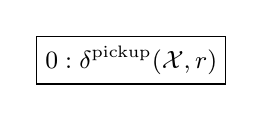
\begin{tikzpicture}
\small
\matrix[nodes={minimum size=6mm}] {
  \node[draw] {$0:\delta^\textrm{pickup}(\mathcal{X},r)$};\\
};
\end{tikzpicture}

where $r$ is the request identified by {\Tt{}rid\nwendquote} (param. 1).\\
\textbf{Side Effects:} none.\\
\textbf{Throws:} {\Tt{}SQLException\nwendquote} if database failure is encountered.\\
\bottomrule
\end{tabular}
\nwenddocs{}\nwbegincode{56}\sublabel{NW1Dx1yV-3eFrmK-1}\nwmargintag{{\nwtagstyle{}\subpageref{NW1Dx1yV-3eFrmK-1}}}\moddef{Read: DBQueryRequestDurationPickup(2)~{\nwtagstyle{}\subpageref{NW1Dx1yV-3eFrmK-1}}}\endmoddef\nwstartdeflinemarkup\nwusesondefline{\\{NW46kjAM-Oyob-1}}\nwenddeflinemarkup
int[] \nwlinkedidentc{DBQueryRequestDurationPickup}{NW1Dx1yV-3eFrmK-1}(final int rid, boolean flag_usecache) throws SQLException \{
  if (flag_usecache) \{
    return new int[] \{ this.duration_requests_pickup.containsKey(rid)
        ? this.duration_requests_pickup.get(rid)
        : 0 \};
  \} else \{
    try (\LA{}Open \code{}conn\edoc{}~{\nwtagstyle{}\subpageref{NW1ODIS0-JT1v9-1}}\RA{}) \{
      return \nwlinkedidentc{PSQuery}{NW1ODIS0-yHOIP-1}(conn, "\nwlinkedidentc{S118}{NW1ODIS0-npyw7-1}", 1, rid);
    \} catch (SQLException e) \{
      throw e;
    \}
  \}
\}
\nwindexdefn{\nwixident{DBQueryRequestDurationPickup}}{DBQueryRequestDurationPickup}{NW1Dx1yV-3eFrmK-1}\eatline
\nwused{\\{NW46kjAM-Oyob-1}}\nwidentdefs{\\{{\nwixident{DBQueryRequestDurationPickup}}{DBQueryRequestDurationPickup}}}\nwidentuses{\\{{\nwixident{PSQuery}}{PSQuery}}\\{{\nwixident{S118}}{S118}}}\nwindexuse{\nwixident{PSQuery}}{PSQuery}{NW1Dx1yV-3eFrmK-1}\nwindexuse{\nwixident{S118}}{S118}{NW1Dx1yV-3eFrmK-1}\nwendcode{}\nwbegindocs{57}\nwdocspar
\subsubsection{\texttt{DBQueryRequestDurationTransit}(1)}
\begin{tabular}{p{\textwidth}}
\toprule
\rowcolor{TableTitle}
Method \textcolor{blue}{{\Tt{}\nwlinkedidentq{DBQueryRequestDurationTransit}{NW1Dx1yV-4AGlqr-1}\nwendquote}}(2) returns the
transit duration $\delta^\textrm{transit}(\mathcal{X},r)$
(Eq.~\ref{eq:transit-duration}) of the given request.
A {\Tt{}SQLException\nwendquote} is thrown in case of database failure.\\
\midrule
\textbf{Parameters:}\\
\begin{tabular}{lp{116mm}}
Integer {\Tt{}rid\nwendquote} (param. 1):&request identifier.
\end{tabular}\\
\textbf{Returns:} results of the query flattened into an integer array,
or {\Tt{}null\nwendquote} if no results.

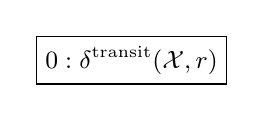
\begin{tikzpicture}
\small
\matrix[nodes={minimum size=6mm}] {
  \node[draw] {$0:\delta^\textrm{transit}(\mathcal{X},r)$};\\
};
\end{tikzpicture}

where $r$ is the request identified by {\Tt{}rid\nwendquote} (param. 1).\\
\textbf{Side Effects:} none.\\
\textbf{Throws:} {\Tt{}SQLException\nwendquote} if database failure is encountered.\\
\bottomrule
\end{tabular}
\nwenddocs{}\nwbegincode{58}\sublabel{NW1Dx1yV-4AGlqr-1}\nwmargintag{{\nwtagstyle{}\subpageref{NW1Dx1yV-4AGlqr-1}}}\moddef{Read: DBQueryRequestDurationTransit(2)~{\nwtagstyle{}\subpageref{NW1Dx1yV-4AGlqr-1}}}\endmoddef\nwstartdeflinemarkup\nwusesondefline{\\{NW46kjAM-Oyob-1}}\nwenddeflinemarkup
int[] \nwlinkedidentc{DBQueryRequestDurationTransit}{NW1Dx1yV-4AGlqr-1}(final int rid, boolean flag_usecache) throws SQLException \{
  if (flag_usecache) \{
    return new int[] \{ this.duration_requests_transit.containsKey(rid)
        ? this.duration_requests_transit.get(rid)
        : 0 \};
  \} else \{
    try (\LA{}Open \code{}conn\edoc{}~{\nwtagstyle{}\subpageref{NW1ODIS0-JT1v9-1}}\RA{}) \{
      return \nwlinkedidentc{PSQuery}{NW1ODIS0-yHOIP-1}(conn, "\nwlinkedidentc{S120}{NW1ODIS0-z4eLL-1}", 1, rid);
    \} catch (SQLException e) \{
      throw e;
    \}
  \}
\}
\nwindexdefn{\nwixident{DBQueryRequestDurationTransit}}{DBQueryRequestDurationTransit}{NW1Dx1yV-4AGlqr-1}\eatline
\nwused{\\{NW46kjAM-Oyob-1}}\nwidentdefs{\\{{\nwixident{DBQueryRequestDurationTransit}}{DBQueryRequestDurationTransit}}}\nwidentuses{\\{{\nwixident{PSQuery}}{PSQuery}}\\{{\nwixident{S120}}{S120}}}\nwindexuse{\nwixident{PSQuery}}{PSQuery}{NW1Dx1yV-4AGlqr-1}\nwindexuse{\nwixident{S120}}{S120}{NW1Dx1yV-4AGlqr-1}\nwendcode{}\nwbegindocs{59}\nwdocspar
\subsubsection{\texttt{DBQueryRequestDurationTravel}(2)}
\begin{tabular}{p{\textwidth}}
\toprule
\rowcolor{TableTitle}
Method \textcolor{blue}{{\Tt{}\nwlinkedidentq{DBQueryRequestDurationTravel}{NW1Dx1yV-3DU2jC-1}\nwendquote}}(2) returns the
travel duration $\delta^\textrm{travel}(\mathcal{X},r)$
(Eq.~\ref{eq:travel-duration}) of the given request.
A {\Tt{}SQLException\nwendquote} is thrown in case of database failure.\\
\midrule
\textbf{Parameters:}\\
\begin{tabular}{lp{116mm}}
Integer {\Tt{}rid\nwendquote} (param. 1):&request identifier.
\end{tabular}\\
\textbf{Returns:} results of the query flattened into an integer array,
or {\Tt{}null\nwendquote} if no results.

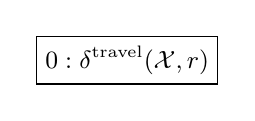
\begin{tikzpicture}
\small
\matrix[nodes={minimum size=6mm}] {
  \node[draw] {$0:\delta^\textrm{travel}(\mathcal{X},r)$};\\
};
\end{tikzpicture}

where $r$ is the request identified by {\Tt{}rid\nwendquote} (param. 1).\\
\textbf{Side Effects:} none.\\
\textbf{Throws:} {\Tt{}SQLException\nwendquote} if database failure is encountered.\\
\bottomrule
\end{tabular}
\nwenddocs{}\nwbegincode{60}\sublabel{NW1Dx1yV-3DU2jC-1}\nwmargintag{{\nwtagstyle{}\subpageref{NW1Dx1yV-3DU2jC-1}}}\moddef{Read: DBQueryRequestDurationTravel(2)~{\nwtagstyle{}\subpageref{NW1Dx1yV-3DU2jC-1}}}\endmoddef\nwstartdeflinemarkup\nwusesondefline{\\{NW46kjAM-Oyob-1}}\nwenddeflinemarkup
int[] \nwlinkedidentc{DBQueryRequestDurationTravel}{NW1Dx1yV-3DU2jC-1}(final int rid, boolean flag_usecache) throws SQLException \{
  if (flag_usecache) \{
    return new int[] \{ this.duration_requests_travel.containsKey(rid)
        ? this.duration_requests_travel.get(rid)
        : 0 \};
  \} else \{
    try (\LA{}Open \code{}conn\edoc{}~{\nwtagstyle{}\subpageref{NW1ODIS0-JT1v9-1}}\RA{}) \{
      return \nwlinkedidentc{PSQuery}{NW1ODIS0-yHOIP-1}(conn, "\nwlinkedidentc{S122}{NW1ODIS0-1S1jbv-1}", 1, rid);
    \} catch (SQLException e) \{
      throw e;
    \}
  \}
\}
\nwindexdefn{\nwixident{DBQueryRequestDurationTravel}}{DBQueryRequestDurationTravel}{NW1Dx1yV-3DU2jC-1}\eatline
\nwused{\\{NW46kjAM-Oyob-1}}\nwidentdefs{\\{{\nwixident{DBQueryRequestDurationTravel}}{DBQueryRequestDurationTravel}}}\nwidentuses{\\{{\nwixident{PSQuery}}{PSQuery}}\\{{\nwixident{S122}}{S122}}}\nwindexuse{\nwixident{PSQuery}}{PSQuery}{NW1Dx1yV-3DU2jC-1}\nwindexuse{\nwixident{S122}}{S122}{NW1Dx1yV-3DU2jC-1}\nwendcode{}\nwbegindocs{61}\nwdocspar
\subsubsection{\texttt{DBQueryRequestTimeOfDeparture}(1)}
\begin{tabular}{p{\textwidth}}
\toprule
\rowcolor{TableTitle}
Method \textcolor{blue}{{\Tt{}\nwlinkedidentq{DBQueryRequestTimeOfDeparture}{NW1Dx1yV-dlG5g-1}\nwendquote}}(1) returns the
departure time $t^\textrm{depart}(\mathcal{X},r)$
(Eq.~\ref{eq:departure-time}) of the given request.
A {\Tt{}SQLException\nwendquote} is thrown in case of database failure.\\
\midrule
\textbf{Parameters:}\\
\begin{tabular}{lp{116mm}}
Integer {\Tt{}rid\nwendquote} (param. 1):&request identifier.
\end{tabular}\\
\textbf{Returns:} results of the query flattened into an integer array,
or {\Tt{}null\nwendquote} if no results.

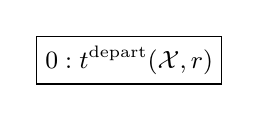
\begin{tikzpicture}
\small
\matrix[nodes={minimum size=6mm}] {
  \node[draw] {$0:t^\textrm{depart}(\mathcal{X},r)$};\\
};
\end{tikzpicture}

where $r$ is the request identified by {\Tt{}rid\nwendquote} (param. 1).\\
\textbf{Side Effects:} none.\\
\textbf{Throws:} {\Tt{}SQLException\nwendquote} if database failure is encountered.\\
\bottomrule
\end{tabular}
\nwenddocs{}\nwbegincode{62}\sublabel{NW1Dx1yV-dlG5g-1}\nwmargintag{{\nwtagstyle{}\subpageref{NW1Dx1yV-dlG5g-1}}}\moddef{Read: DBQueryRequestTimeOfDeparture(1)~{\nwtagstyle{}\subpageref{NW1Dx1yV-dlG5g-1}}}\endmoddef\nwstartdeflinemarkup\nwusesondefline{\\{NW46kjAM-Oyob-1}}\nwenddeflinemarkup
int[] \nwlinkedidentc{DBQueryRequestTimeOfDeparture}{NW1Dx1yV-dlG5g-1}(final int rid) throws SQLException \{
  try (\LA{}Open \code{}conn\edoc{}~{\nwtagstyle{}\subpageref{NW1ODIS0-JT1v9-1}}\RA{}) \{
    return \nwlinkedidentc{PSQuery}{NW1ODIS0-yHOIP-1}(conn, "\nwlinkedidentc{S124}{NW1ODIS0-9hFnf-1}", 1, rid);
  \} catch (SQLException e) \{
    throw e;
  \}
\}
\nwindexdefn{\nwixident{DBQueryRequestTimeOfDeparture}}{DBQueryRequestTimeOfDeparture}{NW1Dx1yV-dlG5g-1}\eatline
\nwused{\\{NW46kjAM-Oyob-1}}\nwidentdefs{\\{{\nwixident{DBQueryRequestTimeOfDeparture}}{DBQueryRequestTimeOfDeparture}}}\nwidentuses{\\{{\nwixident{PSQuery}}{PSQuery}}\\{{\nwixident{S124}}{S124}}}\nwindexuse{\nwixident{PSQuery}}{PSQuery}{NW1Dx1yV-dlG5g-1}\nwindexuse{\nwixident{S124}}{S124}{NW1Dx1yV-dlG5g-1}\nwendcode{}\nwbegindocs{63}\begin{tabular}{p{\textwidth}}
\toprule
\rowcolor{TableTitle}
Method \textcolor{blue}{{\Tt{}\nwlinkedidentq{queryRequestTimeOfDeparture}{NW1Dx1yV-JMT2Q-1}\nwendquote}}(1) wraps {\Tt{}\nwlinkedidentq{DBQueryRequestTimeOfDeparture}{NW1Dx1yV-dlG5g-1}\nwendquote}(1).\\
\bottomrule
\end{tabular}
\nwenddocs{}\nwbegincode{64}\sublabel{NW1Dx1yV-JMT2Q-1}\nwmargintag{{\nwtagstyle{}\subpageref{NW1Dx1yV-JMT2Q-1}}}\moddef{Read: queryRequestTimeOfDeparture(1)~{\nwtagstyle{}\subpageref{NW1Dx1yV-JMT2Q-1}}}\endmoddef\nwstartdeflinemarkup\nwusesondefline{\\{NW3hMOhb-2u8vSA-1}}\nwenddeflinemarkup
int[] \nwlinkedidentc{queryRequestTimeOfDeparture}{NW1Dx1yV-JMT2Q-1}(final int rid) throws SQLException \{
  int[] output = storage.\nwlinkedidentc{DBQueryRequestTimeOfDeparture}{NW1Dx1yV-dlG5g-1}(rid);
  return output;
\}
\nwindexdefn{\nwixident{queryRequestTimeOfDeparture}}{queryRequestTimeOfDeparture}{NW1Dx1yV-JMT2Q-1}\eatline
\nwused{\\{NW3hMOhb-2u8vSA-1}}\nwidentdefs{\\{{\nwixident{queryRequestTimeOfDeparture}}{queryRequestTimeOfDeparture}}}\nwidentuses{\\{{\nwixident{DBQueryRequestTimeOfDeparture}}{DBQueryRequestTimeOfDeparture}}}\nwindexuse{\nwixident{DBQueryRequestTimeOfDeparture}}{DBQueryRequestTimeOfDeparture}{NW1Dx1yV-JMT2Q-1}\nwendcode{}\nwbegindocs{65}\nwdocspar
\subsubsection{\texttt{DBQueryRequestTimeOfArrival}(1)}
\begin{tabular}{p{\textwidth}}
\toprule
\rowcolor{TableTitle}
Method \textcolor{blue}{{\Tt{}\nwlinkedidentq{DBQueryRequestTimeOfArrival}{NW1Dx1yV-cz5yf-1}\nwendquote}}(1) returns the
arrival time $t^\textrm{arrive}(\mathcal{X},r)$
(Eq.~\ref{eq:arrival-time}) of the given request.
A {\Tt{}SQLException\nwendquote} is thrown in case of database failure.\\
\midrule
\textbf{Parameters:}\\
\begin{tabular}{lp{116mm}}
Integer {\Tt{}rid\nwendquote} (param. 1):&request identifier.
\end{tabular}\\
\textbf{Returns:} results of the query flattened into an integer array,
or {\Tt{}null\nwendquote} if no results.

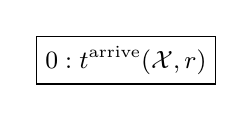
\begin{tikzpicture}
\small
\matrix[nodes={minimum size=6mm}] {
  \node[draw] {$0:t^\textrm{arrive}(\mathcal{X},r)$};\\
};
\end{tikzpicture}

where $r$ is the request identified by {\Tt{}rid\nwendquote} (param. 1).\\
\textbf{Side Effects:} none.\\
\textbf{Throws:} {\Tt{}SQLException\nwendquote} if database failure is encountered.\\
\bottomrule
\end{tabular}
\nwenddocs{}\nwbegincode{66}\sublabel{NW1Dx1yV-cz5yf-1}\nwmargintag{{\nwtagstyle{}\subpageref{NW1Dx1yV-cz5yf-1}}}\moddef{Read: DBQueryRequestTimeOfArrival(1)~{\nwtagstyle{}\subpageref{NW1Dx1yV-cz5yf-1}}}\endmoddef\nwstartdeflinemarkup\nwusesondefline{\\{NW46kjAM-Oyob-1}}\nwenddeflinemarkup
int[] \nwlinkedidentc{DBQueryRequestTimeOfArrival}{NW1Dx1yV-cz5yf-1}(final int rid) throws SQLException \{
  try (\LA{}Open \code{}conn\edoc{}~{\nwtagstyle{}\subpageref{NW1ODIS0-JT1v9-1}}\RA{}) \{
    return \nwlinkedidentc{PSQuery}{NW1ODIS0-yHOIP-1}(conn, "\nwlinkedidentc{S126}{NW1ODIS0-25Tygt-1}", 1, rid);
  \} catch (SQLException e) \{
    throw e;
  \}
\}
\nwindexdefn{\nwixident{DBQueryRequestTimeOfArrival}}{DBQueryRequestTimeOfArrival}{NW1Dx1yV-cz5yf-1}\eatline
\nwused{\\{NW46kjAM-Oyob-1}}\nwidentdefs{\\{{\nwixident{DBQueryRequestTimeOfArrival}}{DBQueryRequestTimeOfArrival}}}\nwidentuses{\\{{\nwixident{PSQuery}}{PSQuery}}\\{{\nwixident{S126}}{S126}}}\nwindexuse{\nwixident{PSQuery}}{PSQuery}{NW1Dx1yV-cz5yf-1}\nwindexuse{\nwixident{S126}}{S126}{NW1Dx1yV-cz5yf-1}\nwendcode{}\nwbegindocs{67}\begin{tabular}{p{\textwidth}}
\toprule
\rowcolor{TableTitle}
Method \textcolor{blue}{{\Tt{}\nwlinkedidentq{queryRequestTimeOfArrival}{NW1Dx1yV-2DgZiX-1}\nwendquote}}(1) wraps {\Tt{}\nwlinkedidentq{DBQueryRequestTimeOfArrival}{NW1Dx1yV-cz5yf-1}\nwendquote}(1).\\
\bottomrule
\end{tabular}
\nwenddocs{}\nwbegincode{68}\sublabel{NW1Dx1yV-2DgZiX-1}\nwmargintag{{\nwtagstyle{}\subpageref{NW1Dx1yV-2DgZiX-1}}}\moddef{Read: queryRequestTimeOfArrival(1)~{\nwtagstyle{}\subpageref{NW1Dx1yV-2DgZiX-1}}}\endmoddef\nwstartdeflinemarkup\nwusesondefline{\\{NW3hMOhb-2u8vSA-1}}\nwenddeflinemarkup
int[] \nwlinkedidentc{queryRequestTimeOfArrival}{NW1Dx1yV-2DgZiX-1}(final int rid) throws SQLException \{
  int[] output = storage.\nwlinkedidentc{DBQueryRequestTimeOfArrival}{NW1Dx1yV-cz5yf-1}(rid);
  return output;
\}
\nwindexdefn{\nwixident{queryRequestTimeOfArrival}}{queryRequestTimeOfArrival}{NW1Dx1yV-2DgZiX-1}\eatline
\nwused{\\{NW3hMOhb-2u8vSA-1}}\nwidentdefs{\\{{\nwixident{queryRequestTimeOfArrival}}{queryRequestTimeOfArrival}}}\nwidentuses{\\{{\nwixident{DBQueryRequestTimeOfArrival}}{DBQueryRequestTimeOfArrival}}}\nwindexuse{\nwixident{DBQueryRequestTimeOfArrival}}{DBQueryRequestTimeOfArrival}{NW1Dx1yV-2DgZiX-1}\nwendcode{}\nwbegindocs{69}\nwdocspar
\subsubsection{\texttt{DBQueryRequestsCount}(0)}
\begin{tabular}{p{\textwidth}}
\toprule
\rowcolor{TableTitle}
Method \textcolor{blue}{{\Tt{}\nwlinkedidentq{DBQueryRequestsCount}{NW1Dx1yV-3PzevO-1}\nwendquote}}(0) returns the total number
of requests in Table R.
A {\Tt{}SQLException\nwendquote} is thrown in case of database failure.\\
\midrule
\textbf{Parameters:} none.\\
\textbf{Returns:} results of the query flattened into an integer array, or
{\Tt{}null\nwendquote} if no results.

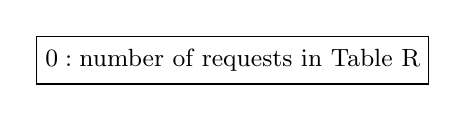
\begin{tikzpicture}
\small
\matrix[nodes={draw,minimum size=6mm}] {
  \node {$0:\textrm{number of requests in Table R}$};\\
};
\end{tikzpicture}\\
\textbf{Side Effects:} none.\\
\textbf{Throws:} {\Tt{}SQLException\nwendquote} if database failure is encountered.\\
\bottomrule
\end{tabular}
\nwenddocs{}\nwbegincode{70}\sublabel{NW1Dx1yV-3PzevO-1}\nwmargintag{{\nwtagstyle{}\subpageref{NW1Dx1yV-3PzevO-1}}}\moddef{Read: DBQueryRequestsCount(0)~{\nwtagstyle{}\subpageref{NW1Dx1yV-3PzevO-1}}}\endmoddef\nwstartdeflinemarkup\nwusesondefline{\\{NW46kjAM-Oyob-1}}\nwenddeflinemarkup
int[] \nwlinkedidentc{DBQueryRequestsCount}{NW1Dx1yV-3PzevO-1}() throws SQLException \{
  // try (\LA{}Open \code{}conn\edoc{}~{\nwtagstyle{}\subpageref{NW1ODIS0-JT1v9-1}}\RA{}) \{
  //   return this.\nwlinkedidentc{PSQuery}{NW1ODIS0-yHOIP-1}(conn, "\nwlinkedidentc{S67}{NW1ODIS0-3PiU32-1}", 1);
  // \} catch (SQLException e) \{
  //   throw e;
  // \}
  return new int[] \{ this.count_requests \};
\}
\nwindexdefn{\nwixident{DBQueryRequestsCount}}{DBQueryRequestsCount}{NW1Dx1yV-3PzevO-1}\eatline
\nwused{\\{NW46kjAM-Oyob-1}}\nwidentdefs{\\{{\nwixident{DBQueryRequestsCount}}{DBQueryRequestsCount}}}\nwidentuses{\\{{\nwixident{PSQuery}}{PSQuery}}\\{{\nwixident{S67}}{S67}}}\nwindexuse{\nwixident{PSQuery}}{PSQuery}{NW1Dx1yV-3PzevO-1}\nwindexuse{\nwixident{S67}}{S67}{NW1Dx1yV-3PzevO-1}\nwendcode{}\nwbegindocs{71}\begin{tabular}{p{\textwidth}}
\toprule
\rowcolor{TableTitle}
Method \textcolor{blue}{{\Tt{}\nwlinkedidentq{queryRequestsCount}{NW1Dx1yV-4WSGXN-1}\nwendquote}}(0) wraps {\Tt{}\nwlinkedidentq{DBQueryRequestsCount}{NW1Dx1yV-3PzevO-1}\nwendquote}(0).\\
\bottomrule
\end{tabular}
\nwenddocs{}\nwbegincode{72}\sublabel{NW1Dx1yV-4WSGXN-1}\nwmargintag{{\nwtagstyle{}\subpageref{NW1Dx1yV-4WSGXN-1}}}\moddef{Read: queryRequestsCount(0)~{\nwtagstyle{}\subpageref{NW1Dx1yV-4WSGXN-1}}}\endmoddef\nwstartdeflinemarkup\nwusesondefline{\\{NW3hMOhb-2u8vSA-1}}\nwenddeflinemarkup
int[] \nwlinkedidentc{queryRequestsCount}{NW1Dx1yV-4WSGXN-1}() throws SQLException \{
  int[] output = storage.\nwlinkedidentc{DBQueryRequestsCount}{NW1Dx1yV-3PzevO-1}();
  return output;
\}
\nwindexdefn{\nwixident{queryRequestsCount}}{queryRequestsCount}{NW1Dx1yV-4WSGXN-1}\eatline
\nwused{\\{NW3hMOhb-2u8vSA-1}}\nwidentdefs{\\{{\nwixident{queryRequestsCount}}{queryRequestsCount}}}\nwidentuses{\\{{\nwixident{DBQueryRequestsCount}}{DBQueryRequestsCount}}}\nwindexuse{\nwixident{DBQueryRequestsCount}}{DBQueryRequestsCount}{NW1Dx1yV-4WSGXN-1}\nwendcode{}\nwbegindocs{73}\nwdocspar
\subsubsection{\texttt{DBQueryRequestsCountActive}(1)}
\nwenddocs{}\nwbegincode{74}\sublabel{NW1Dx1yV-4VamdV-1}\nwmargintag{{\nwtagstyle{}\subpageref{NW1Dx1yV-4VamdV-1}}}\moddef{Read: DBQueryRequestsCountActive(1)~{\nwtagstyle{}\subpageref{NW1Dx1yV-4VamdV-1}}}\endmoddef\nwstartdeflinemarkup\nwusesondefline{\\{NW46kjAM-Oyob-1}}\nwenddeflinemarkup
int[] \nwlinkedidentc{DBQueryRequestsCountActive}{NW1Dx1yV-4VamdV-1}(final int t) throws SQLException \{
  try (\LA{}Open \code{}conn\edoc{}~{\nwtagstyle{}\subpageref{NW1ODIS0-JT1v9-1}}\RA{}) \{
    return this.\nwlinkedidentc{PSQuery}{NW1ODIS0-yHOIP-1}(conn, "\nwlinkedidentc{S161}{NW1ODIS0-3X647v-1}", 1, t, t, t);
  \} catch (SQLException e) \{
    throw e;
  \}
\}
\nwindexdefn{\nwixident{DBQueryRequestsCountActive}}{DBQueryRequestsCountActive}{NW1Dx1yV-4VamdV-1}\eatline
\nwused{\\{NW46kjAM-Oyob-1}}\nwidentdefs{\\{{\nwixident{DBQueryRequestsCountActive}}{DBQueryRequestsCountActive}}}\nwidentuses{\\{{\nwixident{PSQuery}}{PSQuery}}\\{{\nwixident{S161}}{S161}}}\nwindexuse{\nwixident{PSQuery}}{PSQuery}{NW1Dx1yV-4VamdV-1}\nwindexuse{\nwixident{S161}}{S161}{NW1Dx1yV-4VamdV-1}\nwendcode{}\nwbegincode{75}\sublabel{NW1Dx1yV-3PNRV9-1}\nwmargintag{{\nwtagstyle{}\subpageref{NW1Dx1yV-3PNRV9-1}}}\moddef{Read: queryRequestsCountActive(1)~{\nwtagstyle{}\subpageref{NW1Dx1yV-3PNRV9-1}}}\endmoddef\nwstartdeflinemarkup\nwusesondefline{\\{NW3hMOhb-2u8vSA-1}}\nwenddeflinemarkup
int[] \nwlinkedidentc{queryRequestsCountActive}{NW1Dx1yV-3PNRV9-1}(final int t) throws SQLException \{
  int[] output = storage.\nwlinkedidentc{DBQueryRequestsCountActive}{NW1Dx1yV-4VamdV-1}(t);
  return output;
\}
\nwindexdefn{\nwixident{queryRequestsCountActive}}{queryRequestsCountActive}{NW1Dx1yV-3PNRV9-1}\eatline
\nwused{\\{NW3hMOhb-2u8vSA-1}}\nwidentdefs{\\{{\nwixident{queryRequestsCountActive}}{queryRequestsCountActive}}}\nwidentuses{\\{{\nwixident{DBQueryRequestsCountActive}}{DBQueryRequestsCountActive}}}\nwindexuse{\nwixident{DBQueryRequestsCountActive}}{DBQueryRequestsCountActive}{NW1Dx1yV-3PNRV9-1}\nwendcode{}\nwbegindocs{76}\nwdocspar
\subsubsection{\texttt{DBQueryRequestsCountAppeared}(0)}
\nwenddocs{}\nwbegincode{77}\sublabel{NW1Dx1yV-2RWxZw-1}\nwmargintag{{\nwtagstyle{}\subpageref{NW1Dx1yV-2RWxZw-1}}}\moddef{Read: DBQueryRequestsCountAppeared(0)~{\nwtagstyle{}\subpageref{NW1Dx1yV-2RWxZw-1}}}\endmoddef\nwstartdeflinemarkup\nwenddeflinemarkup
int[] \nwlinkedidentc{DBQueryRequestsCountAppeared}{NW1Dx1yV-2RWxZw-1}() throws SQLException \{
  int[] output = new int[] \{ \};
  // ...
  return output;
\}
\nwindexdefn{\nwixident{DBQueryRequestsCountAppeared}}{DBQueryRequestsCountAppeared}{NW1Dx1yV-2RWxZw-1}\eatline
\nwnotused{Read: DBQueryRequestsCountAppeared(0)}\nwidentdefs{\\{{\nwixident{DBQueryRequestsCountAppeared}}{DBQueryRequestsCountAppeared}}}\nwendcode{}\nwbegincode{78}\sublabel{NW1Dx1yV-2tAOFY-1}\nwmargintag{{\nwtagstyle{}\subpageref{NW1Dx1yV-2tAOFY-1}}}\moddef{Read: queryRequestsCountAppeared(0)~{\nwtagstyle{}\subpageref{NW1Dx1yV-2tAOFY-1}}}\endmoddef\nwstartdeflinemarkup\nwusesondefline{\\{NW3hMOhb-2u8vSA-1}}\nwenddeflinemarkup
int[] \nwlinkedidentc{queryRequestsCountAppeared}{NW1Dx1yV-2tAOFY-1}() throws SQLException \{
  int[] output = new int[] \{ this.lu_rseen.size() \};
  return output;
\}
\nwindexdefn{\nwixident{queryRequestsCountAppeared}}{queryRequestsCountAppeared}{NW1Dx1yV-2tAOFY-1}\eatline
\nwused{\\{NW3hMOhb-2u8vSA-1}}\nwidentdefs{\\{{\nwixident{queryRequestsCountAppeared}}{queryRequestsCountAppeared}}}\nwendcode{}\nwbegindocs{79}\nwdocspar
\subsubsection{\texttt{DBQueryRequestsCountAssigned}(0)}
\nwenddocs{}\nwbegincode{80}\sublabel{NW1Dx1yV-2r5hKL-1}\nwmargintag{{\nwtagstyle{}\subpageref{NW1Dx1yV-2r5hKL-1}}}\moddef{Read: DBQueryRequestsCountAssigned(0)~{\nwtagstyle{}\subpageref{NW1Dx1yV-2r5hKL-1}}}\endmoddef\nwstartdeflinemarkup\nwusesondefline{\\{NW46kjAM-Oyob-1}}\nwenddeflinemarkup
int[] \nwlinkedidentc{DBQueryRequestsCountAssigned}{NW1Dx1yV-2r5hKL-1}() throws SQLException \{
  return new int[] \{ this.count_assigned \};
\}
\nwindexdefn{\nwixident{DBQueryRequestsCountAssigned}}{DBQueryRequestsCountAssigned}{NW1Dx1yV-2r5hKL-1}\eatline
\nwused{\\{NW46kjAM-Oyob-1}}\nwidentdefs{\\{{\nwixident{DBQueryRequestsCountAssigned}}{DBQueryRequestsCountAssigned}}}\nwendcode{}\nwbegincode{81}\sublabel{NW1Dx1yV-2P1rxl-1}\nwmargintag{{\nwtagstyle{}\subpageref{NW1Dx1yV-2P1rxl-1}}}\moddef{Read: queryRequestsCountAssigned(0)~{\nwtagstyle{}\subpageref{NW1Dx1yV-2P1rxl-1}}}\endmoddef\nwstartdeflinemarkup\nwusesondefline{\\{NW3hMOhb-2u8vSA-1}}\nwenddeflinemarkup
int[] \nwlinkedidentc{queryRequestsCountAssigned}{NW1Dx1yV-2P1rxl-1}() throws SQLException \{
  int[] output = storage.\nwlinkedidentc{DBQueryRequestsCountAssigned}{NW1Dx1yV-2r5hKL-1}();
  return output;
\}
\nwindexdefn{\nwixident{queryRequestsCountAssigned}}{queryRequestsCountAssigned}{NW1Dx1yV-2P1rxl-1}\eatline
\nwused{\\{NW3hMOhb-2u8vSA-1}}\nwidentdefs{\\{{\nwixident{queryRequestsCountAssigned}}{queryRequestsCountAssigned}}}\nwidentuses{\\{{\nwixident{DBQueryRequestsCountAssigned}}{DBQueryRequestsCountAssigned}}}\nwindexuse{\nwixident{DBQueryRequestsCountAssigned}}{DBQueryRequestsCountAssigned}{NW1Dx1yV-2P1rxl-1}\nwendcode{}\nwbegindocs{82}\nwdocspar
\subsubsection{\texttt{DBQueryRequestsCountCompleted}(1)}
\nwenddocs{}\nwbegincode{83}\sublabel{NW1Dx1yV-4GK84S-1}\nwmargintag{{\nwtagstyle{}\subpageref{NW1Dx1yV-4GK84S-1}}}\moddef{Read: DBQueryRequestsCountCompleted(1)~{\nwtagstyle{}\subpageref{NW1Dx1yV-4GK84S-1}}}\endmoddef\nwstartdeflinemarkup\nwusesondefline{\\{NW46kjAM-Oyob-1}}\nwenddeflinemarkup
int[] \nwlinkedidentc{DBQueryRequestsCountCompleted}{NW1Dx1yV-4GK84S-1}(final int t) throws SQLException \{
  try (\LA{}Open \code{}conn\edoc{}~{\nwtagstyle{}\subpageref{NW1ODIS0-JT1v9-1}}\RA{}) \{
    return this.\nwlinkedidentc{PSQuery}{NW1ODIS0-yHOIP-1}(conn, "\nwlinkedidentc{S161}{NW1ODIS0-3X647v-1}", 1, t, t, t);
  \} catch (SQLException e) \{
    throw e;
  \}
\}
\nwindexdefn{\nwixident{DBQueryRequestsCountCompleted}}{DBQueryRequestsCountCompleted}{NW1Dx1yV-4GK84S-1}\eatline
\nwused{\\{NW46kjAM-Oyob-1}}\nwidentdefs{\\{{\nwixident{DBQueryRequestsCountCompleted}}{DBQueryRequestsCountCompleted}}}\nwidentuses{\\{{\nwixident{PSQuery}}{PSQuery}}\\{{\nwixident{S161}}{S161}}}\nwindexuse{\nwixident{PSQuery}}{PSQuery}{NW1Dx1yV-4GK84S-1}\nwindexuse{\nwixident{S161}}{S161}{NW1Dx1yV-4GK84S-1}\nwendcode{}\nwbegincode{84}\sublabel{NW1Dx1yV-40OaZy-1}\nwmargintag{{\nwtagstyle{}\subpageref{NW1Dx1yV-40OaZy-1}}}\moddef{Read: queryRequestsCountCompleted(1)~{\nwtagstyle{}\subpageref{NW1Dx1yV-40OaZy-1}}}\endmoddef\nwstartdeflinemarkup\nwusesondefline{\\{NW3hMOhb-2u8vSA-1}}\nwenddeflinemarkup
int[] \nwlinkedidentc{queryRequestsCountCompleted}{NW1Dx1yV-40OaZy-1}(final int t) throws SQLException \{
  int[] output = storage.\nwlinkedidentc{DBQueryRequestsCountCompleted}{NW1Dx1yV-4GK84S-1}(t);
  return output;
\}
\nwindexdefn{\nwixident{queryRequestsCountCompleted}}{queryRequestsCountCompleted}{NW1Dx1yV-40OaZy-1}\eatline
\nwused{\\{NW3hMOhb-2u8vSA-1}}\nwidentdefs{\\{{\nwixident{queryRequestsCountCompleted}}{queryRequestsCountCompleted}}}\nwidentuses{\\{{\nwixident{DBQueryRequestsCountCompleted}}{DBQueryRequestsCountCompleted}}}\nwindexuse{\nwixident{DBQueryRequestsCountCompleted}}{DBQueryRequestsCountCompleted}{NW1Dx1yV-40OaZy-1}\nwendcode{}\nwbegindocs{85}\subsubsection{\texttt{DBQueryRequestsQueued}(1)}
\begin{tabular}{p{\textwidth}}
\toprule
\rowcolor{TableTitle}
Method \textcolor{blue}{{\Tt{}\nwlinkedidentq{DBQueryRequestsQueued}{NW1Dx1yV-4AIMTx-1}\nwendquote}}(1) returns the requests
eligible for assignment at the given time. A request $r$ is ``eligible'' if it
is not assigned at the given time, and if the given time is between the
request's early time $r_\texttt{e}$ and
$(r_\texttt{e}+\texttt{REQUEST\_TIMEOUT})$.
A {\Tt{}SQLException\nwendquote} is thrown in case of database failure.\\
\midrule
\textbf{Parameters:} \\
\begin{tabular}{lp{116mm}}
Integer {\Tt{}t\nwendquote} (param. 1):&a time
\end{tabular}\\
\textbf{Returns:} results of the query flattened into an integer array, or
{\Tt{}null\nwendquote} if no results.

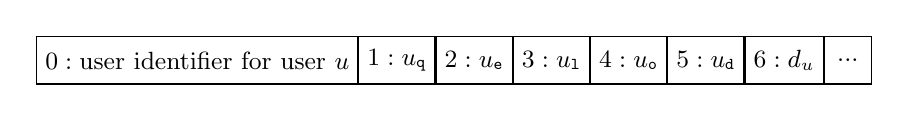
\begin{tikzpicture}
\small
\matrix[nodes={draw,minimum size=6mm}] {
  \node {$0:\textrm{user identifier for user $u$}$};
 &\node {$1:u_\texttt{q}$};
 &\node {$2:u_\texttt{e}$};
 &\node {$3:u_\texttt{l}$};
 &\node {$4:u_\texttt{o}$};
 &\node {$5:u_\texttt{d}$};
 &\node {$6:d_u$};
 &\node {...};\\
};
\end{tikzpicture}\\
\textbf{Side Effects:} none.\\
\textbf{Throws:} {\Tt{}SQLException\nwendquote} if database failure is encountered.\\
\bottomrule
\end{tabular}
\nwenddocs{}\nwbegincode{86}\sublabel{NW1Dx1yV-4AIMTx-1}\nwmargintag{{\nwtagstyle{}\subpageref{NW1Dx1yV-4AIMTx-1}}}\moddef{Read: DBQueryRequestsQueued(1)~{\nwtagstyle{}\subpageref{NW1Dx1yV-4AIMTx-1}}}\endmoddef\nwstartdeflinemarkup\nwusesondefline{\\{NW46kjAM-Oyob-1}}\nwprevnextdefs{\relax}{NW1Dx1yV-4AIMTx-2}\nwenddeflinemarkup
int[] \nwlinkedidentc{DBQueryRequestsQueued}{NW1Dx1yV-4AIMTx-1}(final int t) throws SQLException \{
  try (\LA{}Open \code{}conn\edoc{}~{\nwtagstyle{}\subpageref{NW1ODIS0-JT1v9-1}}\RA{}) \{
\nwindexdefn{\nwixident{DBQueryRequestsQueued}}{DBQueryRequestsQueued}{NW1Dx1yV-4AIMTx-1}\eatline
\nwalsodefined{\\{NW1Dx1yV-4AIMTx-2}\\{NW1Dx1yV-4AIMTx-3}}\nwused{\\{NW46kjAM-Oyob-1}}\nwidentdefs{\\{{\nwixident{DBQueryRequestsQueued}}{DBQueryRequestsQueued}}}\nwendcode{}\nwbegindocs{87}{\small Our approach is to first select all requests where $t$ is between the
request's early time $r_\texttt{e}$ and
$r_\texttt{e}+\texttt{REQUEST\_TIMEOUT}$.  Then, we return a filtered subset of
these requests that are unassigned. As we don't know how many requests will
returned in the end, we initialize a temporary array {\Tt{}temp1\nwendquote} to hold the
pre-filter number of requests.}
\nwenddocs{}\nwbegincode{88}\sublabel{NW1Dx1yV-4AIMTx-2}\nwmargintag{{\nwtagstyle{}\subpageref{NW1Dx1yV-4AIMTx-2}}}\moddef{Read: DBQueryRequestsQueued(1)~{\nwtagstyle{}\subpageref{NW1Dx1yV-4AIMTx-1}}}\plusendmoddef\nwstartdeflinemarkup\nwusesondefline{\\{NW46kjAM-Oyob-1}}\nwprevnextdefs{NW1Dx1yV-4AIMTx-1}{NW1Dx1yV-4AIMTx-3}\nwenddeflinemarkup
    final int[] output = this.\nwlinkedidentc{PSQuery}{NW1ODIS0-yHOIP-1}(conn, "\nwlinkedidentc{S143}{NW1ODIS0-3PFD2J-1}", 7, t, t, REQUEST_TIMEOUT);
    int[] temp1 = new int[output.length];
    int j = 0;
    for (int i = 0; i < (output.length - 6); i += 7) \{
      if (this.lu_rstatus.get(output[i]) == false) \{
        temp1[(j + 0)] = output[(i + 0)];
        temp1[(j + 1)] = output[(i + 1)];
        temp1[(j + 2)] = output[(i + 2)];
        temp1[(j + 3)] = output[(i + 3)];
        temp1[(j + 4)] = output[(i + 4)];
        temp1[(j + 5)] = output[(i + 5)];
        temp1[(j + 6)] = output[(i + 6)];
        j += 7;
      \}
    \}
\nwused{\\{NW46kjAM-Oyob-1}}\nwidentuses{\\{{\nwixident{PSQuery}}{PSQuery}}\\{{\nwixident{S143}}{S143}}}\nwindexuse{\nwixident{PSQuery}}{PSQuery}{NW1Dx1yV-4AIMTx-2}\nwindexuse{\nwixident{S143}}{S143}{NW1Dx1yV-4AIMTx-2}\nwendcode{}\nwbegindocs{89}\nwdocspar
\nwenddocs{}\nwbegincode{90}\sublabel{NW1Dx1yV-4AIMTx-3}\nwmargintag{{\nwtagstyle{}\subpageref{NW1Dx1yV-4AIMTx-3}}}\moddef{Read: DBQueryRequestsQueued(1)~{\nwtagstyle{}\subpageref{NW1Dx1yV-4AIMTx-1}}}\plusendmoddef\nwstartdeflinemarkup\nwusesondefline{\\{NW46kjAM-Oyob-1}}\nwprevnextdefs{NW1Dx1yV-4AIMTx-2}{\relax}\nwenddeflinemarkup
    return Arrays.copyOf(temp1, j);
  \} catch (SQLException e) \{
    throw e;
  \}
\}
\nwused{\\{NW46kjAM-Oyob-1}}\nwendcode{}\nwbegindocs{91}\nwdocspar
\begin{tabular}{p{\textwidth}}
\toprule
\rowcolor{TableTitle}
Method \textcolor{blue}{{\Tt{}\nwlinkedidentq{queryRequestsQueued}{NW1Dx1yV-2FYATt-1}\nwendquote}}(1) wraps {\Tt{}\nwlinkedidentq{DBQueryRequestsQueued}{NW1Dx1yV-4AIMTx-1}\nwendquote}(1).\\
\bottomrule
\end{tabular}
\nwenddocs{}\nwbegincode{92}\sublabel{NW1Dx1yV-2FYATt-1}\nwmargintag{{\nwtagstyle{}\subpageref{NW1Dx1yV-2FYATt-1}}}\moddef{Read: queryRequestsQueued(1)~{\nwtagstyle{}\subpageref{NW1Dx1yV-2FYATt-1}}}\endmoddef\nwstartdeflinemarkup\nwusesondefline{\\{NW3hMOhb-2u8vSA-1}}\nwenddeflinemarkup
int[] \nwlinkedidentc{queryRequestsQueued}{NW1Dx1yV-2FYATt-1}(final int t) throws SQLException \{
  int[] output = storage.\nwlinkedidentc{DBQueryRequestsQueued}{NW1Dx1yV-4AIMTx-1}(t);
  return output;
\}
\nwindexdefn{\nwixident{queryRequestsQueued}}{queryRequestsQueued}{NW1Dx1yV-2FYATt-1}\eatline
\nwused{\\{NW3hMOhb-2u8vSA-1}}\nwidentdefs{\\{{\nwixident{queryRequestsQueued}}{queryRequestsQueued}}}\nwidentuses{\\{{\nwixident{DBQueryRequestsQueued}}{DBQueryRequestsQueued}}}\nwindexuse{\nwixident{DBQueryRequestsQueued}}{DBQueryRequestsQueued}{NW1Dx1yV-2FYATt-1}\nwendcode{}\nwbegindocs{93}\nwdocspar
\subsubsection{\texttt{DBQueryRequestsWaiting}(1)}
\nwenddocs{}\nwbegincode{94}\sublabel{NW1Dx1yV-3TasCr-1}\nwmargintag{{\nwtagstyle{}\subpageref{NW1Dx1yV-3TasCr-1}}}\moddef{Read: DBQueryRequestsWaiting(1)~{\nwtagstyle{}\subpageref{NW1Dx1yV-3TasCr-1}}}\endmoddef\nwstartdeflinemarkup\nwusesondefline{\\{NW46kjAM-Oyob-1}}\nwenddeflinemarkup
int[] \nwlinkedidentc{DBQueryRequestsWaiting}{NW1Dx1yV-3TasCr-1}(final int t) throws SQLException \{
  try (\LA{}Open \code{}conn\edoc{}~{\nwtagstyle{}\subpageref{NW1ODIS0-JT1v9-1}}\RA{}) \{
    return this.\nwlinkedidentc{PSQuery}{NW1ODIS0-yHOIP-1}(conn, "\nwlinkedidentc{S162}{NW1ODIS0-1SEB4d-1}", 2, t, t, REQUEST_TIMEOUT, t);
  \} catch (SQLException e) \{
    throw e;
  \}
\}
\nwindexdefn{\nwixident{DBQueryRequestsWaiting}}{DBQueryRequestsWaiting}{NW1Dx1yV-3TasCr-1}\eatline
\nwused{\\{NW46kjAM-Oyob-1}}\nwidentdefs{\\{{\nwixident{DBQueryRequestsWaiting}}{DBQueryRequestsWaiting}}}\nwidentuses{\\{{\nwixident{PSQuery}}{PSQuery}}\\{{\nwixident{S162}}{S162}}}\nwindexuse{\nwixident{PSQuery}}{PSQuery}{NW1Dx1yV-3TasCr-1}\nwindexuse{\nwixident{S162}}{S162}{NW1Dx1yV-3TasCr-1}\nwendcode{}\nwbegincode{95}\sublabel{NW1Dx1yV-2nvqCn-1}\nwmargintag{{\nwtagstyle{}\subpageref{NW1Dx1yV-2nvqCn-1}}}\moddef{Read: queryRequestsWaiting(1)~{\nwtagstyle{}\subpageref{NW1Dx1yV-2nvqCn-1}}}\endmoddef\nwstartdeflinemarkup\nwusesondefline{\\{NW3hMOhb-2u8vSA-1}}\nwenddeflinemarkup
int[] \nwlinkedidentc{queryRequestsWaiting}{NW1Dx1yV-2nvqCn-1}(final int t) throws SQLException \{
  long A0 = System.currentTimeMillis();
  int[] output = storage.\nwlinkedidentc{DBQueryRequestsWaiting}{NW1Dx1yV-3TasCr-1}(t);
  return output;
\}
\nwindexdefn{\nwixident{queryRequestsWaiting}}{queryRequestsWaiting}{NW1Dx1yV-2nvqCn-1}\eatline
\nwused{\\{NW3hMOhb-2u8vSA-1}}\nwidentdefs{\\{{\nwixident{queryRequestsWaiting}}{queryRequestsWaiting}}}\nwidentuses{\\{{\nwixident{DBQueryRequestsWaiting}}{DBQueryRequestsWaiting}}}\nwindexuse{\nwixident{DBQueryRequestsWaiting}}{DBQueryRequestsWaiting}{NW1Dx1yV-2nvqCn-1}\nwendcode{}\nwbegindocs{96}\nwdocspar
\subsubsection{\texttt{DBQueryServerRoute}(1)}
\begin{tabular}{p{\textwidth}}
\toprule
\rowcolor{TableTitle}
Method \textcolor{blue}{{\Tt{}\nwlinkedidentq{DBQueryServerRoute}{NW1Dx1yV-1cB9Z1-1}\nwendquote}}(1) returns the route for the
given server identified by {\Tt{}sid\nwendquote} (param. 1) at time $t$ (param. 2).
A {\Tt{}SQLException\nwendquote} is thrown in case of database failure.\\
\midrule
\textbf{Parameters:} \\
\begin{tabular}{lp{116mm}}
Integer {\Tt{}sid\nwendquote} (param. 1):&server identifier.\\
\end{tabular}
\textbf{Returns:} results of the query flattened into an integer array,
or {\Tt{}null\nwendquote} if no results.

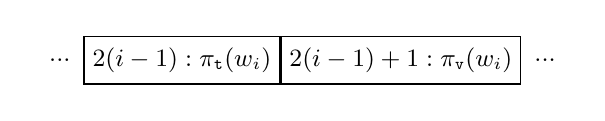
\begin{tikzpicture}
\small
\matrix[nodes={minimum size=6mm}] {
  \node {...};
 &\node[draw] {$2(i-1):\pi_\texttt{t}(w_i)$};
 &\node[draw] {$2(i-1)+1:\pi_\texttt{v}(w_i)$};
 &\node {...};\\
};
\end{tikzpicture}

where $1\leq i\leq |w|$ and $w$ is the route for the given server
identified by {\Tt{}sid\nwendquote} (param. 1).\\
\textbf{Side Effects:} none.\\
\textbf{Throws:} {\Tt{}SQLException\nwendquote} if database failure is encountered.\\
\bottomrule
\end{tabular}
\nwenddocs{}\nwbegincode{97}\sublabel{NW1Dx1yV-1cB9Z1-1}\nwmargintag{{\nwtagstyle{}\subpageref{NW1Dx1yV-1cB9Z1-1}}}\moddef{Read: DBQueryServerRoute(1)~{\nwtagstyle{}\subpageref{NW1Dx1yV-1cB9Z1-1}}}\endmoddef\nwstartdeflinemarkup\nwusesondefline{\\{NW46kjAM-Oyob-1}}\nwenddeflinemarkup
int[] \nwlinkedidentc{DBQueryServerRoute}{NW1Dx1yV-1cB9Z1-1}(final int sid) throws SQLException \{
  try (\LA{}Open \code{}conn\edoc{}~{\nwtagstyle{}\subpageref{NW1ODIS0-JT1v9-1}}\RA{}) \{
    return \nwlinkedidentc{PSQuery}{NW1ODIS0-yHOIP-1}(conn, "\nwlinkedidentc{S60}{NW1ODIS0-9tgZA-1}", 2, sid);
  \} catch (SQLException e) \{
    throw e;
  \}
\}
\nwindexdefn{\nwixident{DBQueryServerRoute}}{DBQueryServerRoute}{NW1Dx1yV-1cB9Z1-1}\eatline
\nwused{\\{NW46kjAM-Oyob-1}}\nwidentdefs{\\{{\nwixident{DBQueryServerRoute}}{DBQueryServerRoute}}}\nwidentuses{\\{{\nwixident{PSQuery}}{PSQuery}}\\{{\nwixident{S60}}{S60}}}\nwindexuse{\nwixident{PSQuery}}{PSQuery}{NW1Dx1yV-1cB9Z1-1}\nwindexuse{\nwixident{S60}}{S60}{NW1Dx1yV-1cB9Z1-1}\nwendcode{}\nwbegindocs{98}\begin{tabular}{p{\textwidth}}
\toprule
\rowcolor{TableTitle}
Method \textcolor{blue}{{\Tt{}\nwlinkedidentq{queryServerRoute}{NW1Dx1yV-3INKD2-1}\nwendquote}}(1) wraps {\Tt{}\nwlinkedidentq{DBQueryServerRoute}{NW1Dx1yV-1cB9Z1-1}\nwendquote}(1).\\
\bottomrule
\end{tabular}
\nwenddocs{}\nwbegincode{99}\sublabel{NW1Dx1yV-3INKD2-1}\nwmargintag{{\nwtagstyle{}\subpageref{NW1Dx1yV-3INKD2-1}}}\moddef{Read: queryServerRoute(1)~{\nwtagstyle{}\subpageref{NW1Dx1yV-3INKD2-1}}}\endmoddef\nwstartdeflinemarkup\nwusesondefline{\\{NW3hMOhb-2u8vSA-1}}\nwenddeflinemarkup
int[] \nwlinkedidentc{queryServerRoute}{NW1Dx1yV-3INKD2-1}(final int sid) throws SQLException \{
  int[] output = storage.\nwlinkedidentc{DBQueryServerRoute}{NW1Dx1yV-1cB9Z1-1}(sid);
  return output;
\}
\nwindexdefn{\nwixident{queryServerRoute}}{queryServerRoute}{NW1Dx1yV-3INKD2-1}\eatline
\nwused{\\{NW3hMOhb-2u8vSA-1}}\nwidentdefs{\\{{\nwixident{queryServerRoute}}{queryServerRoute}}}\nwidentuses{\\{{\nwixident{DBQueryServerRoute}}{DBQueryServerRoute}}}\nwindexuse{\nwixident{DBQueryServerRoute}}{DBQueryServerRoute}{NW1Dx1yV-3INKD2-1}\nwendcode{}\nwbegindocs{100}\nwdocspar
\subsubsection{\texttt{DBQueryServerRouteRemaining}(2)}
\begin{tabular}{p{\textwidth}}
\toprule
\rowcolor{TableTitle}
Method \textcolor{blue}{{\Tt{}\nwlinkedidentq{DBQueryServerRouteRemaining}{NW1Dx1yV-4JTjfI-1}\nwendquote}}(2) returns the
remaining route for the given server at the given time.
A {\Tt{}SQLException\nwendquote} is thrown in case of database failure.\\
\midrule
\textbf{Parameters:} \\
\begin{tabular}{lp{116mm}}
Integer {\Tt{}sid\nwendquote} (param. 1):&server identifier.\\
Integer {\Tt{}t\nwendquote} (param. 2):&a time.\\
\end{tabular}
\textbf{Returns:} results of the query flattened into an integer array,
or {\Tt{}null\nwendquote} if no results.

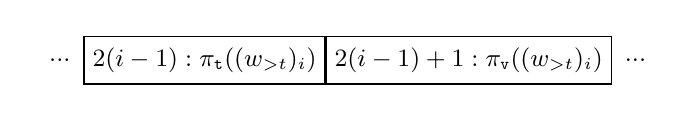
\begin{tikzpicture}
\small
\matrix[nodes={minimum size=6mm}] {
  \node {...};
 &\node[draw] {$2(i-1):\pi_\texttt{t}({(w_{>t}})_i)$};
 &\node[draw] {$2(i-1)+1:\pi_\texttt{v}({(w_{>t}})_i)$};
 &\node {...};\\
};
\end{tikzpicture}

where $1\leq i\leq |w_{>t}|$ and $w_{>t}$ is the remaining route for the
given server identified by {\Tt{}sid\nwendquote} (param. 1) at time $t$ (param. 2).\\
\textbf{Side Effects:} none.\\
\textbf{Throws:} {\Tt{}SQLException\nwendquote} if database failure is encountered.\\
\bottomrule
\end{tabular}
\nwenddocs{}\nwbegincode{101}\sublabel{NW1Dx1yV-4JTjfI-1}\nwmargintag{{\nwtagstyle{}\subpageref{NW1Dx1yV-4JTjfI-1}}}\moddef{Read: DBQueryServerRouteRemaining(2)~{\nwtagstyle{}\subpageref{NW1Dx1yV-4JTjfI-1}}}\endmoddef\nwstartdeflinemarkup\nwusesondefline{\\{NW46kjAM-Oyob-1}}\nwenddeflinemarkup
int[] \nwlinkedidentc{DBQueryServerRouteRemaining}{NW1Dx1yV-4JTjfI-1}(final int sid, final int t) throws SQLException \{
  try (\LA{}Open \code{}conn\edoc{}~{\nwtagstyle{}\subpageref{NW1ODIS0-JT1v9-1}}\RA{}) \{
    return \nwlinkedidentc{PSQuery}{NW1ODIS0-yHOIP-1}(conn, "\nwlinkedidentc{S129}{NW1ODIS0-44X5Zr-1}", 2, sid, t);
  \} catch (SQLException e) \{
    throw e;
  \}
\}
\nwindexdefn{\nwixident{DBQueryServerRouteRemaining}}{DBQueryServerRouteRemaining}{NW1Dx1yV-4JTjfI-1}\eatline
\nwused{\\{NW46kjAM-Oyob-1}}\nwidentdefs{\\{{\nwixident{DBQueryServerRouteRemaining}}{DBQueryServerRouteRemaining}}}\nwidentuses{\\{{\nwixident{PSQuery}}{PSQuery}}\\{{\nwixident{S129}}{S129}}}\nwindexuse{\nwixident{PSQuery}}{PSQuery}{NW1Dx1yV-4JTjfI-1}\nwindexuse{\nwixident{S129}}{S129}{NW1Dx1yV-4JTjfI-1}\nwendcode{}\nwbegindocs{102}\begin{tabular}{p{\textwidth}}
\toprule
\rowcolor{TableTitle}
Method \textcolor{blue}{{\Tt{}\nwlinkedidentq{queryServerRouteRemaining}{NW1Dx1yV-3EQWyS-1}\nwendquote}}(2) wraps {\Tt{}\nwlinkedidentq{DBQueryServerRouteRemaining}{NW1Dx1yV-4JTjfI-1}\nwendquote}(2).\\
\bottomrule
\end{tabular}
\nwenddocs{}\nwbegincode{103}\sublabel{NW1Dx1yV-3EQWyS-1}\nwmargintag{{\nwtagstyle{}\subpageref{NW1Dx1yV-3EQWyS-1}}}\moddef{Read: queryServerRouteRemaining(2)~{\nwtagstyle{}\subpageref{NW1Dx1yV-3EQWyS-1}}}\endmoddef\nwstartdeflinemarkup\nwusesondefline{\\{NW3hMOhb-2u8vSA-1}\\{NW1y1NkR-2Rlctf-1}}\nwenddeflinemarkup
int[] \nwlinkedidentc{queryServerRouteRemaining}{NW1Dx1yV-3EQWyS-1}(final int sid, final int t) throws SQLException \{
  int[] output = this.storage.\nwlinkedidentc{DBQueryServerRouteRemaining}{NW1Dx1yV-4JTjfI-1}(sid, t);
  return output;
\}
\nwindexdefn{\nwixident{queryServerRouteRemaining}}{queryServerRouteRemaining}{NW1Dx1yV-3EQWyS-1}\eatline
\nwused{\\{NW3hMOhb-2u8vSA-1}\\{NW1y1NkR-2Rlctf-1}}\nwidentdefs{\\{{\nwixident{queryServerRouteRemaining}}{queryServerRouteRemaining}}}\nwidentuses{\\{{\nwixident{DBQueryServerRouteRemaining}}{DBQueryServerRouteRemaining}}}\nwindexuse{\nwixident{DBQueryServerRouteRemaining}}{DBQueryServerRouteRemaining}{NW1Dx1yV-3EQWyS-1}\nwendcode{}\nwbegindocs{104}\nwdocspar

\subsubsection{\texttt{DBQueryServerRouteActive}(1)}
Gets the ``active'' route, used for Desktop interpolation. The active route
includes the last-visited vertex, the ``active'' vertex that the server is
currently traveling to, and the next vertex after the active vertex.
\nwenddocs{}\nwbegincode{105}\sublabel{NW1Dx1yV-4IICVC-1}\nwmargintag{{\nwtagstyle{}\subpageref{NW1Dx1yV-4IICVC-1}}}\moddef{Read: DBQueryServerRouteActive(1)~{\nwtagstyle{}\subpageref{NW1Dx1yV-4IICVC-1}}}\endmoddef\nwstartdeflinemarkup\nwusesondefline{\\{NW46kjAM-Oyob-1}}\nwenddeflinemarkup
int[] \nwlinkedidentc{DBQueryServerRouteActive}{NW1Dx1yV-4IICVC-1}(final int sid) throws SQLException \{
  try (\LA{}Open \code{}conn\edoc{}~{\nwtagstyle{}\subpageref{NW1ODIS0-JT1v9-1}}\RA{}) \{
    return \nwlinkedidentc{PSQuery}{NW1ODIS0-yHOIP-1}(conn, "\nwlinkedidentc{S152}{NW1ODIS0-1SnVrH-1}", 2, sid, this.lu_lvt.get(sid), 3);
  \} catch (SQLException e) \{
    throw e;
  \}
\}
\nwindexdefn{\nwixident{DBQueryServerRouteActive}}{DBQueryServerRouteActive}{NW1Dx1yV-4IICVC-1}\eatline
\nwused{\\{NW46kjAM-Oyob-1}}\nwidentdefs{\\{{\nwixident{DBQueryServerRouteActive}}{DBQueryServerRouteActive}}}\nwidentuses{\\{{\nwixident{PSQuery}}{PSQuery}}\\{{\nwixident{S152}}{S152}}}\nwindexuse{\nwixident{PSQuery}}{PSQuery}{NW1Dx1yV-4IICVC-1}\nwindexuse{\nwixident{S152}}{S152}{NW1Dx1yV-4IICVC-1}\nwendcode{}\nwbegincode{106}\sublabel{NW1Dx1yV-oGnJX-1}\nwmargintag{{\nwtagstyle{}\subpageref{NW1Dx1yV-oGnJX-1}}}\moddef{Read: queryServerRouteActive(1)~{\nwtagstyle{}\subpageref{NW1Dx1yV-oGnJX-1}}}\endmoddef\nwstartdeflinemarkup\nwusesondefline{\\{NW3hMOhb-2u8vSA-1}\\{NW1y1NkR-2Rlctf-1}}\nwenddeflinemarkup
int[] \nwlinkedidentc{queryServerRouteActive}{NW1Dx1yV-oGnJX-1}(final int sid) throws SQLException \{
  int[] output = this.storage.\nwlinkedidentc{DBQueryServerRouteActive}{NW1Dx1yV-4IICVC-1}(sid);
  return output;
\}
\nwindexdefn{\nwixident{queryServerRouteActive}}{queryServerRouteActive}{NW1Dx1yV-oGnJX-1}\eatline
\nwused{\\{NW3hMOhb-2u8vSA-1}\\{NW1y1NkR-2Rlctf-1}}\nwidentdefs{\\{{\nwixident{queryServerRouteActive}}{queryServerRouteActive}}}\nwidentuses{\\{{\nwixident{DBQueryServerRouteActive}}{DBQueryServerRouteActive}}}\nwindexuse{\nwixident{DBQueryServerRouteActive}}{DBQueryServerRouteActive}{NW1Dx1yV-oGnJX-1}\nwendcode{}\nwbegindocs{107}\nwdocspar
\subsubsection{\texttt{DBQueryServerSchedule}(1)}
\begin{tabular}{p{\textwidth}}
\toprule
\rowcolor{TableTitle}
Method \textcolor{blue}{{\Tt{}\nwlinkedidentq{DBQueryServerSchedule}{NW1Dx1yV-71ppP-1}\nwendquote}}(1) returns the schedule
for the given server.
A {\Tt{}SQLException\nwendquote} is thrown in case of database failure.\\
\midrule
\textbf{Parameters:} \\
\begin{tabular}{lp{116mm}}
Integer {\Tt{}sid\nwendquote} (param. 1):&server identifier.\\
\end{tabular}
\textbf{Returns:} results of the query flattened into an integer array,
or {\Tt{}null\nwendquote} if no results.

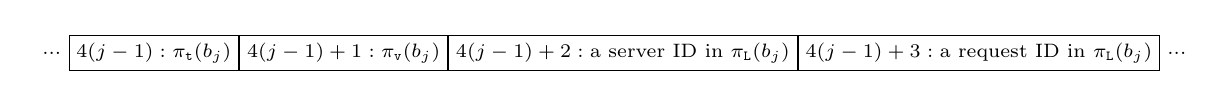
\begin{tikzpicture}
\scriptsize
\matrix[nodes={}] {
  \node {...};
 &\node[draw] {$4(j-1):\pi_\texttt{t}(b_j)$};
 &\node[draw] {$4(j-1)+1:\pi_\texttt{v}(b_j)$};
 &\node[draw] {$4(j-1)+2:\textrm{a server ID in }\pi_\texttt{L}(b_j)$};
 &\node[draw] {$4(j-1)+3:\textrm{a request ID in }\pi_\texttt{L}(b_j)$};
 &\node {...};\\
};
\end{tikzpicture}

where $1\leq j\leq |b|$ and $b$ is the schedule for the
given server  identified by {\Tt{}sid\nwendquote} (param. 1).
If a label is empty (\textit{e.g.} not all waypoints will have a server
identifier in their label set), the element will be 0. If a waypoint has
multiple labels, the waypoint will be written once for each of the labels.
The returned sequence is in time-ascending order but \textbf{is not guaranteed}
to be in the same order as the actual pick-ups and drop-offs, \textit{e.g.} if a
waypoint has multiple labels with some indicating pick-ups and some indicating
drop-offs, the ordering of these waypoints is uncertain.\\
\textbf{Side Effects:} none.\\
\textbf{Throws:} {\Tt{}SQLException\nwendquote} if database failure is encountered.\\
\bottomrule
\end{tabular}
\nwenddocs{}\nwbegincode{108}\sublabel{NW1Dx1yV-71ppP-1}\nwmargintag{{\nwtagstyle{}\subpageref{NW1Dx1yV-71ppP-1}}}\moddef{Read: DBQueryServerSchedule(1)~{\nwtagstyle{}\subpageref{NW1Dx1yV-71ppP-1}}}\endmoddef\nwstartdeflinemarkup\nwusesondefline{\\{NW46kjAM-Oyob-1}}\nwenddeflinemarkup
int[] \nwlinkedidentc{DBQueryServerSchedule}{NW1Dx1yV-71ppP-1}(final int sid) throws SQLException \{
  try (\LA{}Open \code{}conn\edoc{}~{\nwtagstyle{}\subpageref{NW1ODIS0-JT1v9-1}}\RA{}) \{
    return \nwlinkedidentc{PSQuery}{NW1ODIS0-yHOIP-1}(conn, "\nwlinkedidentc{S61}{NW1ODIS0-4e4a2O-1}", 4, sid);
  \} catch (SQLException e) \{
    throw e;
  \}
\}
\nwindexdefn{\nwixident{DBQueryServerSchedule}}{DBQueryServerSchedule}{NW1Dx1yV-71ppP-1}\eatline
\nwused{\\{NW46kjAM-Oyob-1}}\nwidentdefs{\\{{\nwixident{DBQueryServerSchedule}}{DBQueryServerSchedule}}}\nwidentuses{\\{{\nwixident{PSQuery}}{PSQuery}}\\{{\nwixident{S61}}{S61}}}\nwindexuse{\nwixident{PSQuery}}{PSQuery}{NW1Dx1yV-71ppP-1}\nwindexuse{\nwixident{S61}}{S61}{NW1Dx1yV-71ppP-1}\nwendcode{}\nwbegindocs{109}\begin{tabular}{p{\textwidth}}
\toprule
\rowcolor{TableTitle}
Method \textcolor{blue}{{\Tt{}\nwlinkedidentq{queryServerSchedule}{NW1Dx1yV-2vGK9z-1}\nwendquote}}(1) wraps {\Tt{}\nwlinkedidentq{DBQueryServerSchedule}{NW1Dx1yV-71ppP-1}\nwendquote}(1).\\
\bottomrule
\end{tabular}
\nwenddocs{}\nwbegincode{110}\sublabel{NW1Dx1yV-2vGK9z-1}\nwmargintag{{\nwtagstyle{}\subpageref{NW1Dx1yV-2vGK9z-1}}}\moddef{Read: queryServerSchedule(1)~{\nwtagstyle{}\subpageref{NW1Dx1yV-2vGK9z-1}}}\endmoddef\nwstartdeflinemarkup\nwusesondefline{\\{NW3hMOhb-2u8vSA-1}}\nwenddeflinemarkup
int[] \nwlinkedidentc{queryServerSchedule}{NW1Dx1yV-2vGK9z-1}(final int sid) throws SQLException \{
  int[] output = storage.\nwlinkedidentc{DBQueryServerSchedule}{NW1Dx1yV-71ppP-1}(sid);
  return output;
\}
\nwindexdefn{\nwixident{queryServerSchedule}}{queryServerSchedule}{NW1Dx1yV-2vGK9z-1}\eatline
\nwused{\\{NW3hMOhb-2u8vSA-1}}\nwidentdefs{\\{{\nwixident{queryServerSchedule}}{queryServerSchedule}}}\nwidentuses{\\{{\nwixident{DBQueryServerSchedule}}{DBQueryServerSchedule}}}\nwindexuse{\nwixident{DBQueryServerSchedule}}{DBQueryServerSchedule}{NW1Dx1yV-2vGK9z-1}\nwendcode{}\nwbegindocs{111}\nwdocspar
\subsubsection{\texttt{DBQueryServerScheduleRemaining}(2)}
\begin{tabular}{p{\textwidth}}
\toprule
\rowcolor{TableTitle}
Method \textcolor{blue}{{\Tt{}\nwlinkedidentq{DBQueryServerScheduleRemaining}{NW1Dx1yV-48DsrJ-1}\nwendquote}}(2) returns the
remaining schedule for the given server at the given time.
A {\Tt{}SQLException\nwendquote} is thrown in case of database failure.\\
\midrule
\textbf{Parameters:} \\
\begin{tabular}{lp{116mm}}
Integer {\Tt{}sid\nwendquote} (param. 1):&server identifier.\\
Integer {\Tt{}t\nwendquote} (param. 2):&a time.\\
\end{tabular}
\textbf{Returns:} results of the query flattened into an integer array,
or {\Tt{}null\nwendquote} if no results.

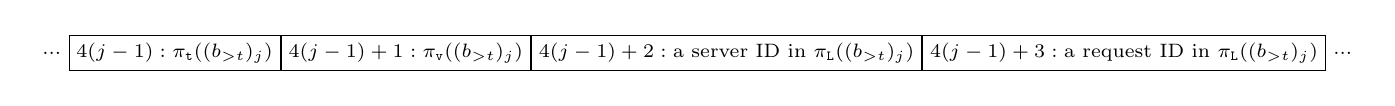
\begin{tikzpicture}
\scriptsize
\matrix[nodes={}] {
  \node {...};
 &\node[draw] {$4(j-1):\pi_\texttt{t}((b_{>t})_j)$};
 &\node[draw] {$4(j-1)+1:\pi_\texttt{v}((b_{>t})_j)$};
 &\node[draw] {$4(j-1)+2:\textrm{a server ID in }\pi_\texttt{L}((b_{>t})_j)$};
 &\node[draw] {$4(j-1)+3:\textrm{a request ID in }\pi_\texttt{L}((b_{>t})_j)$};
 &\node {...};\\
};
\end{tikzpicture}

where $1\leq j\leq |b_{>t}|$ and $b_{>t}$ is the remaining schedule for the
given server identified by {\Tt{}sid\nwendquote} (param. 1) at time $t$ (param. 2).
If a label is empty (\textit{e.g.} not all waypoints will have a server
identifier in their label set), the element will be 0. If a waypoint has
multiple labels, the waypoint will be written once for each of the labels.
The returned sequence is in time-ascending order and \textbf{is guaranteed}
to be in the same order as the actual pick-ups and drop-offs.\\
\textbf{Side Effects:} none.\\
\textbf{Throws:} {\Tt{}SQLException\nwendquote} if database failure is encountered.\\
\bottomrule
\end{tabular}
\nwenddocs{}\nwbegincode{112}\sublabel{NW1Dx1yV-48DsrJ-1}\nwmargintag{{\nwtagstyle{}\subpageref{NW1Dx1yV-48DsrJ-1}}}\moddef{Read: DBQueryServerScheduleRemaining(2)~{\nwtagstyle{}\subpageref{NW1Dx1yV-48DsrJ-1}}}\endmoddef\nwstartdeflinemarkup\nwusesondefline{\\{NW46kjAM-Oyob-1}}\nwenddeflinemarkup
int[] \nwlinkedidentc{DBQueryServerScheduleRemaining}{NW1Dx1yV-48DsrJ-1}(final int sid, final int t)
throws SQLException \{
  int[] output = new int[] \{ \};
  try (\LA{}Open \code{}conn\edoc{}~{\nwtagstyle{}\subpageref{NW1ODIS0-JT1v9-1}}\RA{}) \{
    int[] temp = \nwlinkedidentc{PSQuery}{NW1ODIS0-yHOIP-1}(conn, "\nwlinkedidentc{S144}{NW1ODIS0-9zboZ-1}", 3, sid, t);
    output = new int[(4*temp.length/3 + 4)];
    int j = 0;
    for (int i = 0; i < (temp.length - 2); i += 3) \{
      output[(j + 0)] = temp[(i + 0)];
      output[(j + 1)] = temp[(i + 1)];
      output[(j + 2)] = 0;
      output[(j + 3)] = temp[(i + 2)];
      j += 4;
    \}
    temp = \nwlinkedidentc{PSQuery}{NW1ODIS0-yHOIP-1}(conn, "\nwlinkedidentc{S145}{NW1ODIS0-4eAVHn-1}", 2, sid);
    output[(j + 0)] = temp[0];
    output[(j + 1)] = temp[1];
    output[(j + 2)] = sid;
    output[(j + 3)] = 0;
  \} catch (SQLException e) \{
    throw e;
  \}
  return output;
\}
\nwindexdefn{\nwixident{DBQueryServerScheduleRemaining}}{DBQueryServerScheduleRemaining}{NW1Dx1yV-48DsrJ-1}\eatline
\nwused{\\{NW46kjAM-Oyob-1}}\nwidentdefs{\\{{\nwixident{DBQueryServerScheduleRemaining}}{DBQueryServerScheduleRemaining}}}\nwidentuses{\\{{\nwixident{PSQuery}}{PSQuery}}\\{{\nwixident{S144}}{S144}}\\{{\nwixident{S145}}{S145}}}\nwindexuse{\nwixident{PSQuery}}{PSQuery}{NW1Dx1yV-48DsrJ-1}\nwindexuse{\nwixident{S144}}{S144}{NW1Dx1yV-48DsrJ-1}\nwindexuse{\nwixident{S145}}{S145}{NW1Dx1yV-48DsrJ-1}\nwendcode{}\nwbegindocs{113}\begin{tabular}{p{\textwidth}}
\toprule
\rowcolor{TableTitle}
Method \textcolor{blue}{{\Tt{}\nwlinkedidentq{queryServerScheduleRemaining}{NW1Dx1yV-2iMTVQ-1}\nwendquote}}(2) wraps {\Tt{}\nwlinkedidentq{DBQueryServerScheduleRemaining}{NW1Dx1yV-48DsrJ-1}\nwendquote}(2).\\
\bottomrule
\end{tabular}
\nwenddocs{}\nwbegincode{114}\sublabel{NW1Dx1yV-2iMTVQ-1}\nwmargintag{{\nwtagstyle{}\subpageref{NW1Dx1yV-2iMTVQ-1}}}\moddef{Read: queryServerScheduleRemaining(2)~{\nwtagstyle{}\subpageref{NW1Dx1yV-2iMTVQ-1}}}\endmoddef\nwstartdeflinemarkup\nwusesondefline{\\{NW1y1NkR-2Rlctf-1}}\nwenddeflinemarkup
int[] \nwlinkedidentc{queryServerScheduleRemaining}{NW1Dx1yV-2iMTVQ-1}(final int sid, final int t) throws SQLException \{
  int[] output = this.storage.\nwlinkedidentc{DBQueryServerScheduleRemaining}{NW1Dx1yV-48DsrJ-1}(sid, t);
  return output;
\}
\nwindexdefn{\nwixident{queryServerScheduleRemaining}}{queryServerScheduleRemaining}{NW1Dx1yV-2iMTVQ-1}\eatline
\nwused{\\{NW1y1NkR-2Rlctf-1}}\nwidentdefs{\\{{\nwixident{queryServerScheduleRemaining}}{queryServerScheduleRemaining}}}\nwidentuses{\\{{\nwixident{DBQueryServerScheduleRemaining}}{DBQueryServerScheduleRemaining}}}\nwindexuse{\nwixident{DBQueryServerScheduleRemaining}}{DBQueryServerScheduleRemaining}{NW1Dx1yV-2iMTVQ-1}\nwendcode{}\nwbegindocs{115}\nwdocspar
\subsubsection{\texttt{DBQueryServerLoadMax}(2)}
\begin{tabular}{p{\textwidth}}
\toprule
\rowcolor{TableTitle}
Method \textcolor{blue}{{\Tt{}\nwlinkedidentq{DBQueryServerLoadMax}{NW1Dx1yV-1O34Sj-1}\nwendquote}}(2) returns the maximum load
for the given server at the given time. The ``maximum load'' is equal to the
load burden $Q(\mathcal{X},s,t)$ \emph{plus} the sum of the loads of the
requests that are dropped off by the server at $t$. In other words it is the
number of occupied seats at $t$ before any drop-offs happen.
A {\Tt{}SQLException\nwendquote} is thrown in case of database failure.\\
\midrule
\textbf{Parameters:} \\
\begin{tabular}{lp{116mm}}
Integer {\Tt{}sid\nwendquote} (param. 1):&server identifier.\\
Integer {\Tt{}t\nwendquote} (param. 2):&a time.\\
\end{tabular}
\textbf{Returns:} results of the query flattened into an integer array,
or {\Tt{}null\nwendquote} if no results.

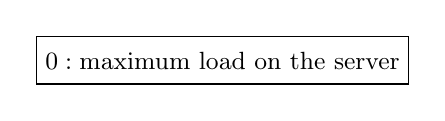
\begin{tikzpicture}
\small
\matrix[nodes={draw,minimum size=6mm}] {
  \node {$0:\textrm{maximum load on the server}$};\\
};
\end{tikzpicture}\\
\textbf{Side Effects:} none.\\
\textbf{Throws:} {\Tt{}SQLException\nwendquote} if database failure is encountered.\\
\bottomrule
\end{tabular}
\nwenddocs{}\nwbegincode{116}\sublabel{NW1Dx1yV-1O34Sj-1}\nwmargintag{{\nwtagstyle{}\subpageref{NW1Dx1yV-1O34Sj-1}}}\moddef{Read: DBQueryServerLoadMax(2)~{\nwtagstyle{}\subpageref{NW1Dx1yV-1O34Sj-1}}}\endmoddef\nwstartdeflinemarkup\nwusesondefline{\\{NW46kjAM-Oyob-1}}\nwenddeflinemarkup
int[] \nwlinkedidentc{DBQueryServerLoadMax}{NW1Dx1yV-1O34Sj-1}(final int sid, final int t) throws SQLException \{
  try (\LA{}Open \code{}conn\edoc{}~{\nwtagstyle{}\subpageref{NW1ODIS0-JT1v9-1}}\RA{}) \{
    return \nwlinkedidentc{PSQuery}{NW1ODIS0-yHOIP-1}(conn, "\nwlinkedidentc{S73}{NW1ODIS0-2U8wBI-1}", 1, sid, t);
  \} catch (SQLException e) \{
    throw e;
  \}
\}
\nwindexdefn{\nwixident{DBQueryServerLoadMax}}{DBQueryServerLoadMax}{NW1Dx1yV-1O34Sj-1}\eatline
\nwused{\\{NW46kjAM-Oyob-1}}\nwidentdefs{\\{{\nwixident{DBQueryServerLoadMax}}{DBQueryServerLoadMax}}}\nwidentuses{\\{{\nwixident{PSQuery}}{PSQuery}}\\{{\nwixident{S73}}{S73}}}\nwindexuse{\nwixident{PSQuery}}{PSQuery}{NW1Dx1yV-1O34Sj-1}\nwindexuse{\nwixident{S73}}{S73}{NW1Dx1yV-1O34Sj-1}\nwendcode{}\nwbegindocs{117}\begin{tabular}{p{\textwidth}}
\toprule
\rowcolor{TableTitle}
Method \textcolor{blue}{{\Tt{}\nwlinkedidentq{queryServerLoadMax}{NW1Dx1yV-7Mvmo-1}\nwendquote}}(2) wraps {\Tt{}\nwlinkedidentq{DBQueryServerLoadMax}{NW1Dx1yV-1O34Sj-1}\nwendquote}(2).\\
\bottomrule
\end{tabular}
\nwenddocs{}\nwbegincode{118}\sublabel{NW1Dx1yV-7Mvmo-1}\nwmargintag{{\nwtagstyle{}\subpageref{NW1Dx1yV-7Mvmo-1}}}\moddef{Read: queryServerLoadMax(2)~{\nwtagstyle{}\subpageref{NW1Dx1yV-7Mvmo-1}}}\endmoddef\nwstartdeflinemarkup\nwusesondefline{\\{NW1y1NkR-2Rlctf-1}}\nwenddeflinemarkup
int[] \nwlinkedidentc{queryServerLoadMax}{NW1Dx1yV-7Mvmo-1}(final int sid, final int t) throws SQLException \{
  int[] output = this.storage.\nwlinkedidentc{DBQueryServerLoadMax}{NW1Dx1yV-1O34Sj-1}(sid, t);
  return output;
\}
\nwindexdefn{\nwixident{queryServerLoadMax}}{queryServerLoadMax}{NW1Dx1yV-7Mvmo-1}\eatline
\nwused{\\{NW1y1NkR-2Rlctf-1}}\nwidentdefs{\\{{\nwixident{queryServerLoadMax}}{queryServerLoadMax}}}\nwidentuses{\\{{\nwixident{DBQueryServerLoadMax}}{DBQueryServerLoadMax}}}\nwindexuse{\nwixident{DBQueryServerLoadMax}}{DBQueryServerLoadMax}{NW1Dx1yV-7Mvmo-1}\nwendcode{}\nwbegindocs{119}\nwdocspar
\subsubsection{\texttt{DBQueryServerCapacityViolations}(4)}
\begin{tabular}{p{\textwidth}}
\toprule
\rowcolor{TableTitle}
Method \textcolor{blue}{{\Tt{}\nwlinkedidentq{DBQueryServerCapacityViolations}{NW1Dx1yV-hzOIm-1}\nwendquote}}(4) returns the
number of schedule events in excess of server capacity within a given time
range if a new load were applied during that range.
A {\Tt{}SQLException\nwendquote} is thrown in case of database failure.\\
\midrule
\textbf{Parameters:} \\
\begin{tabular}{lp{116mm}}
Integer {\Tt{}sid\nwendquote} (param. 1):&server identifier.\\
Integer {\Tt{}rq\nwendquote} (param. 2):&additional load to apply.\\
Integer {\Tt{}tp\nwendquote} (param. 3):&start time.\\
Integer {\Tt{}td\nwendquote} (param. 4):&end time.\\
\end{tabular}\\
\textbf{Returns:} results of the query flattened into an integer array,
or {\Tt{}null\nwendquote} if no results.

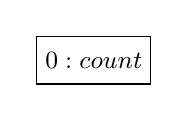
\begin{tikzpicture}
\small
\matrix[nodes={minimum size=6mm}] {
  \node[draw] {$0:count$};\\
};
\end{tikzpicture}

where $count$ is the number of events in exceeding server capacity.\\
\textbf{Side Effects:} none.\\
\textbf{Throws:} {\Tt{}SQLException\nwendquote} if database failure is encountered.\\
\bottomrule
\end{tabular}
\nwenddocs{}\nwbegincode{120}\sublabel{NW1Dx1yV-hzOIm-1}\nwmargintag{{\nwtagstyle{}\subpageref{NW1Dx1yV-hzOIm-1}}}\moddef{Read: DBQueryServerCapacityViolations(4)~{\nwtagstyle{}\subpageref{NW1Dx1yV-hzOIm-1}}}\endmoddef\nwstartdeflinemarkup\nwusesondefline{\\{NW46kjAM-Oyob-1}}\nwenddeflinemarkup
int[] \nwlinkedidentc{DBQueryServerCapacityViolations}{NW1Dx1yV-hzOIm-1}(final int sid,
    final int rq, final int tp, final int td) throws SQLException \{
  try (\LA{}Open \code{}conn\edoc{}~{\nwtagstyle{}\subpageref{NW1ODIS0-JT1v9-1}}\RA{}) \{
    return \nwlinkedidentc{PSQuery}{NW1ODIS0-yHOIP-1}(conn, "\nwlinkedidentc{S163}{NW1ODIS0-3PiUkF-1}", 1, sid, rq, td, td, tp, td);
  \} catch (SQLException e) \{
    throw e;
  \}
\}
\nwindexdefn{\nwixident{DBQueryServerCapacityViolations}}{DBQueryServerCapacityViolations}{NW1Dx1yV-hzOIm-1}\eatline
\nwused{\\{NW46kjAM-Oyob-1}}\nwidentdefs{\\{{\nwixident{DBQueryServerCapacityViolations}}{DBQueryServerCapacityViolations}}}\nwidentuses{\\{{\nwixident{PSQuery}}{PSQuery}}\\{{\nwixident{S163}}{S163}}}\nwindexuse{\nwixident{PSQuery}}{PSQuery}{NW1Dx1yV-hzOIm-1}\nwindexuse{\nwixident{S163}}{S163}{NW1Dx1yV-hzOIm-1}\nwendcode{}\nwbegincode{121}\sublabel{NW1Dx1yV-3b4wOq-1}\nwmargintag{{\nwtagstyle{}\subpageref{NW1Dx1yV-3b4wOq-1}}}\moddef{Read: queryServerCapacityViolations(4)~{\nwtagstyle{}\subpageref{NW1Dx1yV-3b4wOq-1}}}\endmoddef\nwstartdeflinemarkup\nwusesondefline{\\{NW1y1NkR-2Rlctf-1}}\nwenddeflinemarkup
int[] \nwlinkedidentc{queryServerCapacityViolations}{NW1Dx1yV-3b4wOq-1}(final int sid,
    final int rq, final int tp, final int td) throws SQLException \{
  return this.storage.\nwlinkedidentc{DBQueryServerCapacityViolations}{NW1Dx1yV-hzOIm-1}(sid, rq, tp, td);
\}
\nwindexdefn{\nwixident{queryServerCapacityViolations}}{queryServerCapacityViolations}{NW1Dx1yV-3b4wOq-1}\eatline
\nwused{\\{NW1y1NkR-2Rlctf-1}}\nwidentdefs{\\{{\nwixident{queryServerCapacityViolations}}{queryServerCapacityViolations}}}\nwidentuses{\\{{\nwixident{DBQueryServerCapacityViolations}}{DBQueryServerCapacityViolations}}}\nwindexuse{\nwixident{DBQueryServerCapacityViolations}}{DBQueryServerCapacityViolations}{NW1Dx1yV-3b4wOq-1}\nwendcode{}\nwbegindocs{122}\nwdocspar
\subsubsection{\texttt{DBQueryServerDistance}(2)}
\begin{tabular}{p{\textwidth}}
\toprule
\rowcolor{TableTitle}
Method \textcolor{blue}{{\Tt{}\nwlinkedidentq{DBQueryServerDistance}{NW1Dx1yV-bdI1v-1}\nwendquote}}(2) returns the
travel distance $D(w)$ of the given server.
A {\Tt{}SQLException\nwendquote} is thrown in case of database failure.\\
\midrule
\textbf{Parameters:} \\
\begin{tabular}{lp{116mm}}
Integer {\Tt{}sid\nwendquote} (param. 1):&server identifier.\\
Boolean {\Tt{}flag{\_}usecache\nwendquote} (param. 1):&{\Tt{}false\nwendquote} to force retrieval from database.
\end{tabular}\\
\textbf{Returns:} results of the query flattened into an integer array,
or {\Tt{}null\nwendquote} if no results.

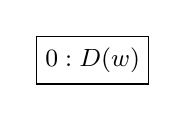
\begin{tikzpicture}
\small
\matrix[nodes={minimum size=6mm}] {
  \node[draw] {$0:D(w)$};\\
};
\end{tikzpicture}

where $w$ is the route of the given server identified by {\Tt{}sid\nwendquote} (param. 1).\\
\textbf{Side Effects:} none.\\
\textbf{Throws:} {\Tt{}SQLException\nwendquote} if database failure is encountered.\\
\bottomrule
\end{tabular}
\nwenddocs{}\nwbegincode{123}\sublabel{NW1Dx1yV-bdI1v-1}\nwmargintag{{\nwtagstyle{}\subpageref{NW1Dx1yV-bdI1v-1}}}\moddef{Read: DBQueryServerDistance(2)~{\nwtagstyle{}\subpageref{NW1Dx1yV-bdI1v-1}}}\endmoddef\nwstartdeflinemarkup\nwusesondefline{\\{NW46kjAM-Oyob-1}}\nwenddeflinemarkup
int[] \nwlinkedidentc{DBQueryServerDistance}{NW1Dx1yV-bdI1v-1}(final int sid, boolean flag_usecache) throws SQLException \{
  if (flag_usecache) \{
    return new int[] \{ this.distance_servers.get(sid) \};
  \} else \{
    try (\LA{}Open \code{}conn\edoc{}~{\nwtagstyle{}\subpageref{NW1ODIS0-JT1v9-1}}\RA{}) \{
      return \nwlinkedidentc{PSQuery}{NW1ODIS0-yHOIP-1}(conn, "\nwlinkedidentc{S104}{NW1ODIS0-A9AGR-1}", 1, sid);
    \} catch (SQLException e) \{
      throw e;
    \}
  \}
\}
\nwindexdefn{\nwixident{DBQueryServerDistance}}{DBQueryServerDistance}{NW1Dx1yV-bdI1v-1}\eatline
\nwused{\\{NW46kjAM-Oyob-1}}\nwidentdefs{\\{{\nwixident{DBQueryServerDistance}}{DBQueryServerDistance}}}\nwidentuses{\\{{\nwixident{PSQuery}}{PSQuery}}\\{{\nwixident{S104}}{S104}}}\nwindexuse{\nwixident{PSQuery}}{PSQuery}{NW1Dx1yV-bdI1v-1}\nwindexuse{\nwixident{S104}}{S104}{NW1Dx1yV-bdI1v-1}\nwendcode{}\nwbegincode{124}\sublabel{NW1Dx1yV-3NhJSl-1}\nwmargintag{{\nwtagstyle{}\subpageref{NW1Dx1yV-3NhJSl-1}}}\moddef{Read: queryServerDistance(2)~{\nwtagstyle{}\subpageref{NW1Dx1yV-3NhJSl-1}}}\endmoddef\nwstartdeflinemarkup\nwusesondefline{\\{NW3hMOhb-2u8vSA-1}}\nwenddeflinemarkup
int[] \nwlinkedidentc{queryServerDistance}{NW1Dx1yV-3NhJSl-1}(final int sid, boolean flag_usecache) throws SQLException \{
  return this.storage.\nwlinkedidentc{DBQueryServerDistance}{NW1Dx1yV-bdI1v-1}(sid, flag_usecache);
\}
\nwindexdefn{\nwixident{queryServerDistance}}{queryServerDistance}{NW1Dx1yV-3NhJSl-1}\eatline
\nwused{\\{NW3hMOhb-2u8vSA-1}}\nwidentdefs{\\{{\nwixident{queryServerDistance}}{queryServerDistance}}}\nwidentuses{\\{{\nwixident{DBQueryServerDistance}}{DBQueryServerDistance}}}\nwindexuse{\nwixident{DBQueryServerDistance}}{DBQueryServerDistance}{NW1Dx1yV-3NhJSl-1}\nwendcode{}\nwbegindocs{125}\nwdocspar
\subsubsection{\texttt{DBQueryServerDistanceRemaining}(2)}
\begin{tabular}{p{\textwidth}}
\toprule
\rowcolor{TableTitle}
Method \textcolor{blue}{{\Tt{}\nwlinkedidentq{DBQueryServerDistanceRemaining}{NW1Dx1yV-23Wg9M-1}\nwendquote}}(2) returns the
remaining distance $D(w_{>t})$ for the given server at the given time.
A {\Tt{}SQLException\nwendquote} is thrown in case of database failure.\\
\midrule
\textbf{Parameters:} \\
\begin{tabular}{lp{116mm}}
Integer {\Tt{}sid\nwendquote} (param. 1):&server identifier.\\
Integer {\Tt{}t\nwendquote} (param. 2):&a time.\\
\end{tabular}
\textbf{Returns:} results of the query flattened into an integer array,
or {\Tt{}null\nwendquote} if no results.

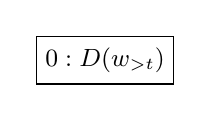
\begin{tikzpicture}
\small
\matrix[nodes={draw,minimum size=6mm}] {
  \node {$0:D(w_{>t})$};\\
};
\end{tikzpicture}

where $w_{>t}$ is the remaining route for the given server identified by {\Tt{}sid\nwendquote} (param. 1).\\
\textbf{Side Effects:} none.\\
\textbf{Throws:} {\Tt{}SQLException\nwendquote} if database failure is encountered.\\
\bottomrule
\end{tabular}
\nwenddocs{}\nwbegincode{126}\sublabel{NW1Dx1yV-23Wg9M-1}\nwmargintag{{\nwtagstyle{}\subpageref{NW1Dx1yV-23Wg9M-1}}}\moddef{Read: DBQueryServerDistanceRemaining(2)~{\nwtagstyle{}\subpageref{NW1Dx1yV-23Wg9M-1}}}\endmoddef\nwstartdeflinemarkup\nwusesondefline{\\{NW46kjAM-Oyob-1}}\nwenddeflinemarkup
int[] \nwlinkedidentc{DBQueryServerDistanceRemaining}{NW1Dx1yV-23Wg9M-1}(final int sid, final int t)
throws SQLException \{
  try (\LA{}Open \code{}conn\edoc{}~{\nwtagstyle{}\subpageref{NW1ODIS0-JT1v9-1}}\RA{}) \{
    return \nwlinkedidentc{PSQuery}{NW1ODIS0-yHOIP-1}(conn, "\nwlinkedidentc{S142}{NW1ODIS0-1RktMh-1}", 1, sid, t);
  \} catch (SQLException e) \{
    throw e;
  \}
\}
\nwindexdefn{\nwixident{DBQueryServerDistanceRemaining}}{DBQueryServerDistanceRemaining}{NW1Dx1yV-23Wg9M-1}\eatline
\nwused{\\{NW46kjAM-Oyob-1}}\nwidentdefs{\\{{\nwixident{DBQueryServerDistanceRemaining}}{DBQueryServerDistanceRemaining}}}\nwidentuses{\\{{\nwixident{PSQuery}}{PSQuery}}\\{{\nwixident{S142}}{S142}}}\nwindexuse{\nwixident{PSQuery}}{PSQuery}{NW1Dx1yV-23Wg9M-1}\nwindexuse{\nwixident{S142}}{S142}{NW1Dx1yV-23Wg9M-1}\nwendcode{}\nwbegindocs{127}\begin{tabular}{p{\textwidth}}
\toprule
\rowcolor{TableTitle}
Method \textcolor{blue}{{\Tt{}\nwlinkedidentq{queryServerDistanceRemaining}{NW1Dx1yV-6TJm1-1}\nwendquote}}(2) wraps {\Tt{}\nwlinkedidentq{DBQueryServerDistanceRemaining}{NW1Dx1yV-23Wg9M-1}\nwendquote}(2).\\
\bottomrule
\end{tabular}
\nwenddocs{}\nwbegincode{128}\sublabel{NW1Dx1yV-6TJm1-1}\nwmargintag{{\nwtagstyle{}\subpageref{NW1Dx1yV-6TJm1-1}}}\moddef{Read: queryServerDistanceRemaining(2)~{\nwtagstyle{}\subpageref{NW1Dx1yV-6TJm1-1}}}\endmoddef\nwstartdeflinemarkup\nwusesondefline{\\{NW1y1NkR-2Rlctf-1}}\nwenddeflinemarkup
int[] \nwlinkedidentc{queryServerDistanceRemaining}{NW1Dx1yV-6TJm1-1}(final int sid, final int t) throws SQLException \{
  int[] output = this.storage.\nwlinkedidentc{DBQueryServerDistanceRemaining}{NW1Dx1yV-23Wg9M-1}(sid, t);
  return output;
\}
\nwindexdefn{\nwixident{queryServerDistanceRemaining}}{queryServerDistanceRemaining}{NW1Dx1yV-6TJm1-1}\eatline
\nwused{\\{NW1y1NkR-2Rlctf-1}}\nwidentdefs{\\{{\nwixident{queryServerDistanceRemaining}}{queryServerDistanceRemaining}}}\nwidentuses{\\{{\nwixident{DBQueryServerDistanceRemaining}}{DBQueryServerDistanceRemaining}}}\nwindexuse{\nwixident{DBQueryServerDistanceRemaining}}{DBQueryServerDistanceRemaining}{NW1Dx1yV-6TJm1-1}\nwendcode{}\nwbegindocs{129}\nwdocspar
\subsubsection{\texttt{DBQueryServerDistanceCruising}(2)}
\begin{tabular}{p{\textwidth}}
\toprule
\rowcolor{TableTitle}
Method \textcolor{blue}{{\Tt{}\nwlinkedidentq{DBQueryServerDistanceCruising}{NW1Dx1yV-4MQ6st-1}\nwendquote}}(2) returns the
cruising distance $D^\textrm{cruise}(\mathcal{X},s)$
(Eq.~\ref{eq:cruising-distance}) of the given server.
A {\Tt{}SQLException\nwendquote} is thrown in case of database failure.\\
\midrule
\textbf{Parameters:}\\
\begin{tabular}{lp{116mm}}
Integer {\Tt{}sid\nwendquote} (param. 1):&server identifier.
\end{tabular}\\
\textbf{Returns:} results of the query flattened into an integer array,
or {\Tt{}null\nwendquote} if no results.

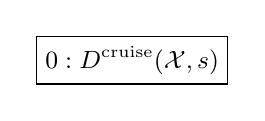
\begin{tikzpicture}
\small
\matrix[nodes={minimum size=6mm}] {
  \node[draw] {$0:D^\textrm{cruise}(\mathcal{X},s)$};\\
};
\end{tikzpicture}

where $s$ is the server identified by {\Tt{}sid\nwendquote} (param. 1).\\
\textbf{Side Effects:} none.\\
\textbf{Throws:} {\Tt{}SQLException\nwendquote} if database failure is encountered.\\
\bottomrule
\end{tabular}
\nwenddocs{}\nwbegincode{130}\sublabel{NW1Dx1yV-4MQ6st-1}\nwmargintag{{\nwtagstyle{}\subpageref{NW1Dx1yV-4MQ6st-1}}}\moddef{Read: DBQueryServerDistanceCruising(2)~{\nwtagstyle{}\subpageref{NW1Dx1yV-4MQ6st-1}}}\endmoddef\nwstartdeflinemarkup\nwusesondefline{\\{NW46kjAM-Oyob-1}}\nwenddeflinemarkup
int[] \nwlinkedidentc{DBQueryServerDistanceCruising}{NW1Dx1yV-4MQ6st-1}(final int sid, boolean flag_usecache) throws SQLException \{
  if (flag_usecache) \{
    return new int [] \{ this.distance_servers_cruising.get(sid) \};
  \} else \{
    try (\LA{}Open \code{}conn\edoc{}~{\nwtagstyle{}\subpageref{NW1ODIS0-JT1v9-1}}\RA{}) \{
      return \nwlinkedidentc{PSQuery}{NW1ODIS0-yHOIP-1}(conn, "\nwlinkedidentc{S106}{NW1ODIS0-25vt9f-1}", 1, sid);
    \} catch (SQLException e) \{
      throw e;
    \}
  \}
\}
\nwindexdefn{\nwixident{DBQueryServerDistanceCruising}}{DBQueryServerDistanceCruising}{NW1Dx1yV-4MQ6st-1}\eatline
\nwused{\\{NW46kjAM-Oyob-1}}\nwidentdefs{\\{{\nwixident{DBQueryServerDistanceCruising}}{DBQueryServerDistanceCruising}}}\nwidentuses{\\{{\nwixident{PSQuery}}{PSQuery}}\\{{\nwixident{S106}}{S106}}}\nwindexuse{\nwixident{PSQuery}}{PSQuery}{NW1Dx1yV-4MQ6st-1}\nwindexuse{\nwixident{S106}}{S106}{NW1Dx1yV-4MQ6st-1}\nwendcode{}\nwbegindocs{131}\nwdocspar
\subsubsection{\texttt{DBQueryServerDistanceService}(2)}
\begin{tabular}{p{\textwidth}}
\toprule
\rowcolor{TableTitle}
Method \textcolor{blue}{{\Tt{}\nwlinkedidentq{DBQueryServerDistanceService}{NW1Dx1yV-1pzTLm-1}\nwendquote}}(2) returns the
service distance $D^\textrm{service}(\mathcal{X},s)$
(Eq.~\ref{eq:service-distance}) of the given server.
A {\Tt{}SQLException\nwendquote} is thrown in case of database failure.\\
\midrule
\textbf{Parameters:}\\
\begin{tabular}{lp{116mm}}
Integer {\Tt{}sid\nwendquote} (param. 1):&server identifier.
\end{tabular}\\
\textbf{Returns:} results of the query flattened into an integer array,
or {\Tt{}null\nwendquote} if no results.

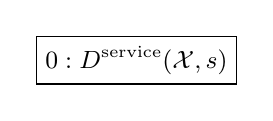
\begin{tikzpicture}
\small
\matrix[nodes={minimum size=6mm}] {
  \node[draw] {$0:D^\textrm{service}(\mathcal{X},s)$};\\
};
\end{tikzpicture}

where $s$ is the server identified by {\Tt{}sid\nwendquote} (param. 1).\\
\textbf{Side Effects:} none.\\
\textbf{Throws:} {\Tt{}SQLException\nwendquote} if database failure is encountered.\\
\bottomrule
\end{tabular}
\nwenddocs{}\nwbegincode{132}\sublabel{NW1Dx1yV-1pzTLm-1}\nwmargintag{{\nwtagstyle{}\subpageref{NW1Dx1yV-1pzTLm-1}}}\moddef{Read: DBQueryServerDistanceService(2)~{\nwtagstyle{}\subpageref{NW1Dx1yV-1pzTLm-1}}}\endmoddef\nwstartdeflinemarkup\nwusesondefline{\\{NW46kjAM-Oyob-1}}\nwenddeflinemarkup
int[] \nwlinkedidentc{DBQueryServerDistanceService}{NW1Dx1yV-1pzTLm-1}(final int sid, boolean flag_usecache) throws SQLException \{
  if (flag_usecache) \{
    return new int [] \{ this.distance_servers.get(sid) - this.distance_servers_cruising.get(sid) \};
  \} else \{
    try (\LA{}Open \code{}conn\edoc{}~{\nwtagstyle{}\subpageref{NW1ODIS0-JT1v9-1}}\RA{}) \{
      return \nwlinkedidentc{PSQuery}{NW1ODIS0-yHOIP-1}(conn, "\nwlinkedidentc{S108}{NW1ODIS0-mtPWF-1}", 1, sid);
    \} catch (SQLException e) \{
      throw e;
    \}
  \}
\}
\nwindexdefn{\nwixident{DBQueryServerDistanceService}}{DBQueryServerDistanceService}{NW1Dx1yV-1pzTLm-1}\eatline
\nwused{\\{NW46kjAM-Oyob-1}}\nwidentdefs{\\{{\nwixident{DBQueryServerDistanceService}}{DBQueryServerDistanceService}}}\nwidentuses{\\{{\nwixident{PSQuery}}{PSQuery}}\\{{\nwixident{S108}}{S108}}}\nwindexuse{\nwixident{PSQuery}}{PSQuery}{NW1Dx1yV-1pzTLm-1}\nwindexuse{\nwixident{S108}}{S108}{NW1Dx1yV-1pzTLm-1}\nwendcode{}\nwbegindocs{133}\nwdocspar
\subsubsection{\texttt{DBQueryServerDurationRemaining}(2)}
\begin{tabular}{p{\textwidth}}
\toprule
\rowcolor{TableTitle}
Method \textcolor{blue}{{\Tt{}\nwlinkedidentq{DBQueryServerDurationRemaining}{NW1Dx1yV-1aOzfQ-1}\nwendquote}}(2) returns the
remaining duration $\delta(w_{>t})$ for the given server at the given time.
A {\Tt{}SQLException\nwendquote} is thrown in case of database failure.\\
\midrule
\textbf{Parameters:} \\
\begin{tabular}{lp{116mm}}
Integer {\Tt{}sid\nwendquote} (param. 1):&server identifier.\\
Integer {\Tt{}t\nwendquote} (param. 2):&a time.\\
\end{tabular}
\textbf{Returns:} results of the query flattened into an integer array,
or {\Tt{}null\nwendquote} if no results.

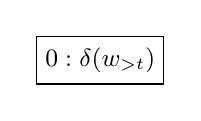
\begin{tikzpicture}
\small
\matrix[nodes={draw,minimum size=6mm}] {
  \node {$0:\delta(w_{>t})$};\\
};
\end{tikzpicture}

where $w_{>t}$ is the remaining route for the given server identified by {\Tt{}sid\nwendquote} (param. 1).\\
\textbf{Side Effects:} none.\\
\textbf{Throws:} {\Tt{}SQLException\nwendquote} if database failure is encountered.\\
\bottomrule
\end{tabular}
\nwenddocs{}\nwbegincode{134}\sublabel{NW1Dx1yV-1aOzfQ-1}\nwmargintag{{\nwtagstyle{}\subpageref{NW1Dx1yV-1aOzfQ-1}}}\moddef{Read: DBQueryServerDurationRemaining(2)~{\nwtagstyle{}\subpageref{NW1Dx1yV-1aOzfQ-1}}}\endmoddef\nwstartdeflinemarkup\nwusesondefline{\\{NW46kjAM-Oyob-1}}\nwenddeflinemarkup
int[] \nwlinkedidentc{DBQueryServerDurationRemaining}{NW1Dx1yV-1aOzfQ-1}(final int sid, final int t)
throws SQLException \{
  try (\LA{}Open \code{}conn\edoc{}~{\nwtagstyle{}\subpageref{NW1ODIS0-JT1v9-1}}\RA{}) \{
    int[] output = \nwlinkedidentc{PSQuery}{NW1ODIS0-yHOIP-1}(conn, "\nwlinkedidentc{S127}{NW1ODIS0-2TKHcJ-1}", 1, sid, t);
    if (output != null) \{
      output[0] -= t;
    \}
    return output;
  \} catch (SQLException e) \{
    throw e;
  \}
\}
\nwindexdefn{\nwixident{DBQueryServerDurationRemaining}}{DBQueryServerDurationRemaining}{NW1Dx1yV-1aOzfQ-1}\eatline
\nwused{\\{NW46kjAM-Oyob-1}}\nwidentdefs{\\{{\nwixident{DBQueryServerDurationRemaining}}{DBQueryServerDurationRemaining}}}\nwidentuses{\\{{\nwixident{PSQuery}}{PSQuery}}\\{{\nwixident{S127}}{S127}}}\nwindexuse{\nwixident{PSQuery}}{PSQuery}{NW1Dx1yV-1aOzfQ-1}\nwindexuse{\nwixident{S127}}{S127}{NW1Dx1yV-1aOzfQ-1}\nwendcode{}\nwbegindocs{135}\begin{tabular}{p{\textwidth}}
\toprule
\rowcolor{TableTitle}
Method \textcolor{blue}{{\Tt{}\nwlinkedidentq{queryServerDurationRemaining}{NW1Dx1yV-e3rqH-1}\nwendquote}}(2) wraps {\Tt{}\nwlinkedidentq{DBQueryServerDurationRemaining}{NW1Dx1yV-1aOzfQ-1}\nwendquote}(2).\\
\bottomrule
\end{tabular}
\nwenddocs{}\nwbegincode{136}\sublabel{NW1Dx1yV-e3rqH-1}\nwmargintag{{\nwtagstyle{}\subpageref{NW1Dx1yV-e3rqH-1}}}\moddef{Read: queryServerDurationRemaining(2)~{\nwtagstyle{}\subpageref{NW1Dx1yV-e3rqH-1}}}\endmoddef\nwstartdeflinemarkup\nwusesondefline{\\{NW1y1NkR-2Rlctf-1}}\nwenddeflinemarkup
int[] \nwlinkedidentc{queryServerDurationRemaining}{NW1Dx1yV-e3rqH-1}(final int sid, final int t) throws SQLException \{
  int[] output = this.storage.\nwlinkedidentc{DBQueryServerDurationRemaining}{NW1Dx1yV-1aOzfQ-1}(sid, t);
  return output;
\}
\nwindexdefn{\nwixident{queryServerDurationRemaining}}{queryServerDurationRemaining}{NW1Dx1yV-e3rqH-1}\eatline
\nwused{\\{NW1y1NkR-2Rlctf-1}}\nwidentdefs{\\{{\nwixident{queryServerDurationRemaining}}{queryServerDurationRemaining}}}\nwidentuses{\\{{\nwixident{DBQueryServerDurationRemaining}}{DBQueryServerDurationRemaining}}}\nwindexuse{\nwixident{DBQueryServerDurationRemaining}}{DBQueryServerDurationRemaining}{NW1Dx1yV-e3rqH-1}\nwendcode{}\nwbegindocs{137}\nwdocspar
\subsubsection{\texttt{DBQueryServerDurationTravel}(2)}
\begin{tabular}{p{\textwidth}}
\toprule
\rowcolor{TableTitle}
Method \textcolor{blue}{{\Tt{}\nwlinkedidentq{DBQueryServerDurationTravel}{NW1Dx1yV-TNQQF-1}\nwendquote}}(2) returns the
travel duration $\delta^\textrm{travel}(\mathcal{X},r)$
(Eq.~\ref{eq:travel-duration}) of the given server.
A {\Tt{}SQLException\nwendquote} is thrown in case of database failure.\\
\midrule
\textbf{Parameters:}\\
\begin{tabular}{lp{116mm}}
Integer {\Tt{}sid\nwendquote} (param. 1):&server identifier.
\end{tabular}\\
\textbf{Returns:} results of the query flattened into an integer array,
or {\Tt{}null\nwendquote} if no results.

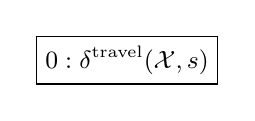
\begin{tikzpicture}
\small
\matrix[nodes={minimum size=6mm}] {
  \node[draw] {$0:\delta^\textrm{travel}(\mathcal{X},s)$};\\
};
\end{tikzpicture}

where $s$ is the server identified by {\Tt{}sid\nwendquote} (param. 1).\\
\textbf{Side Effects:} none.\\
\textbf{Throws:} {\Tt{}SQLException\nwendquote} if database failure is encountered.\\
\bottomrule
\end{tabular}
\nwenddocs{}\nwbegincode{138}\sublabel{NW1Dx1yV-TNQQF-1}\nwmargintag{{\nwtagstyle{}\subpageref{NW1Dx1yV-TNQQF-1}}}\moddef{Read: DBQueryServerDurationTravel(2)~{\nwtagstyle{}\subpageref{NW1Dx1yV-TNQQF-1}}}\endmoddef\nwstartdeflinemarkup\nwusesondefline{\\{NW46kjAM-Oyob-1}}\nwenddeflinemarkup
int[] \nwlinkedidentc{DBQueryServerDurationTravel}{NW1Dx1yV-TNQQF-1}(final int sid, boolean flag_usecache) throws SQLException \{
  if (flag_usecache) \{
    return new int[] \{ this.duration_servers.containsKey(sid)
      ? this.duration_servers.get(sid)
      : 0 \};
  \} else \{
    try (\LA{}Open \code{}conn\edoc{}~{\nwtagstyle{}\subpageref{NW1ODIS0-JT1v9-1}}\RA{}) \{
      return \nwlinkedidentc{PSQuery}{NW1ODIS0-yHOIP-1}(conn, "\nwlinkedidentc{S116}{NW1ODIS0-261fBL-1}", 1, sid);
    \} catch (SQLException e) \{
      throw e;
    \}
  \}
\}
\nwindexdefn{\nwixident{DBQueryServerDurationTravel}}{DBQueryServerDurationTravel}{NW1Dx1yV-TNQQF-1}\eatline
\nwused{\\{NW46kjAM-Oyob-1}}\nwidentdefs{\\{{\nwixident{DBQueryServerDurationTravel}}{DBQueryServerDurationTravel}}}\nwidentuses{\\{{\nwixident{PSQuery}}{PSQuery}}\\{{\nwixident{S116}}{S116}}}\nwindexuse{\nwixident{PSQuery}}{PSQuery}{NW1Dx1yV-TNQQF-1}\nwindexuse{\nwixident{S116}}{S116}{NW1Dx1yV-TNQQF-1}\nwendcode{}\nwbegincode{139}\sublabel{NW1Dx1yV-1DqiB9-1}\nwmargintag{{\nwtagstyle{}\subpageref{NW1Dx1yV-1DqiB9-1}}}\moddef{Read: queryServerDurationTravel(2)~{\nwtagstyle{}\subpageref{NW1Dx1yV-1DqiB9-1}}}\endmoddef\nwstartdeflinemarkup\nwusesondefline{\\{NW1y1NkR-2Rlctf-1}}\nwenddeflinemarkup
int[] \nwlinkedidentc{queryServerDurationTravel}{NW1Dx1yV-1DqiB9-1}(final int sid, boolean flag_usecache) throws SQLException \{
  return storage.\nwlinkedidentc{DBQueryServerDurationTravel}{NW1Dx1yV-TNQQF-1}(sid, flag_usecache);
\}
\nwindexdefn{\nwixident{queryServerDurationTravel}}{queryServerDurationTravel}{NW1Dx1yV-1DqiB9-1}\eatline
\nwused{\\{NW1y1NkR-2Rlctf-1}}\nwidentdefs{\\{{\nwixident{queryServerDurationTravel}}{queryServerDurationTravel}}}\nwidentuses{\\{{\nwixident{DBQueryServerDurationTravel}}{DBQueryServerDurationTravel}}}\nwindexuse{\nwixident{DBQueryServerDurationTravel}}{DBQueryServerDurationTravel}{NW1Dx1yV-1DqiB9-1}\nwendcode{}\nwbegindocs{140}\nwdocspar
\subsubsection{\texttt{DBQueryServerDurationCruising}(2)}
\nwenddocs{}\nwbegincode{141}\sublabel{NW1Dx1yV-1p4hKh-1}\nwmargintag{{\nwtagstyle{}\subpageref{NW1Dx1yV-1p4hKh-1}}}\moddef{Read: DBQueryServerDurationCruising(2)~{\nwtagstyle{}\subpageref{NW1Dx1yV-1p4hKh-1}}}\endmoddef\nwstartdeflinemarkup\nwusesondefline{\\{NW46kjAM-Oyob-1}}\nwenddeflinemarkup
int[] \nwlinkedidentc{DBQueryServerDurationCruising}{NW1Dx1yV-1p4hKh-1}(final int sid, boolean flag_usecache) throws SQLException \{
  if (flag_usecache) \{
    return new int[] \{ this.duration_servers_cruising.get(sid) \};
  \} else \{
    try (\LA{}Open \code{}conn\edoc{}~{\nwtagstyle{}\subpageref{NW1ODIS0-JT1v9-1}}\RA{}) \{
      return \nwlinkedidentc{PSQuery}{NW1ODIS0-yHOIP-1}(conn, "\nwlinkedidentc{S158}{NW1ODIS0-nmTYx-1}", 1, sid, sid);
    \} catch (SQLException e) \{
      throw e;
    \}
  \}
\}
\nwindexdefn{\nwixident{DBQueryServerDurationCruising}}{DBQueryServerDurationCruising}{NW1Dx1yV-1p4hKh-1}\eatline
\nwused{\\{NW46kjAM-Oyob-1}}\nwidentdefs{\\{{\nwixident{DBQueryServerDurationCruising}}{DBQueryServerDurationCruising}}}\nwidentuses{\\{{\nwixident{PSQuery}}{PSQuery}}\\{{\nwixident{S158}}{S158}}}\nwindexuse{\nwixident{PSQuery}}{PSQuery}{NW1Dx1yV-1p4hKh-1}\nwindexuse{\nwixident{S158}}{S158}{NW1Dx1yV-1p4hKh-1}\nwendcode{}\nwbegindocs{142}\nwdocspar
\subsubsection{\texttt{DBQueryServerDurationService}(2)}
\nwenddocs{}\nwbegincode{143}\sublabel{NW1Dx1yV-1spPfd-1}\nwmargintag{{\nwtagstyle{}\subpageref{NW1Dx1yV-1spPfd-1}}}\moddef{Read: DBQueryServerDurationService(2)~{\nwtagstyle{}\subpageref{NW1Dx1yV-1spPfd-1}}}\endmoddef\nwstartdeflinemarkup\nwusesondefline{\\{NW46kjAM-Oyob-1}}\nwenddeflinemarkup
int[] \nwlinkedidentc{DBQueryServerDurationService}{NW1Dx1yV-1spPfd-1}(final int sid, boolean flag_usecache) throws SQLException \{
  if (flag_usecache) \{
    return new int[] \{ (this.duration_servers.get(sid)
        - this.duration_servers_cruising.get(sid)) \};
  \} else \{
    try (\LA{}Open \code{}conn\edoc{}~{\nwtagstyle{}\subpageref{NW1ODIS0-JT1v9-1}}\RA{}) \{
      return \nwlinkedidentc{PSQuery}{NW1ODIS0-yHOIP-1}(conn, "\nwlinkedidentc{S157}{NW1ODIS0-2U63rf-1}", 1, sid);
    \} catch (SQLException e) \{
      throw e;
    \}
  \}
\}
\nwindexdefn{\nwixident{DBQueryServerDurationService}}{DBQueryServerDurationService}{NW1Dx1yV-1spPfd-1}\eatline
\nwused{\\{NW46kjAM-Oyob-1}}\nwidentdefs{\\{{\nwixident{DBQueryServerDurationService}}{DBQueryServerDurationService}}}\nwidentuses{\\{{\nwixident{PSQuery}}{PSQuery}}\\{{\nwixident{S157}}{S157}}}\nwindexuse{\nwixident{PSQuery}}{PSQuery}{NW1Dx1yV-1spPfd-1}\nwindexuse{\nwixident{S157}}{S157}{NW1Dx1yV-1spPfd-1}\nwendcode{}\nwbegindocs{144}\nwdocspar
\subsubsection{\texttt{DBQueryServerTimeOfDeparture}(1)}
\begin{tabular}{p{\textwidth}}
\toprule
\rowcolor{TableTitle}
Method \textcolor{blue}{{\Tt{}\nwlinkedidentq{DBQueryServerTimeOfDeparture}{NW1Dx1yV-3pEbv2-1}\nwendquote}}(1) returns the
departure time $t^\textrm{depart}(\mathcal{X},s)$
(Eq.~\ref{eq:departure-time}) of the given server.
A {\Tt{}SQLException\nwendquote} is thrown in case of database failure.\\
\midrule
\textbf{Parameters:}\\
\begin{tabular}{lp{116mm}}
Integer {\Tt{}sid\nwendquote} (param. 1):&server identifier.
\end{tabular}\\
\textbf{Returns:} results of the query flattened into an integer array,
or {\Tt{}null\nwendquote} if no results.

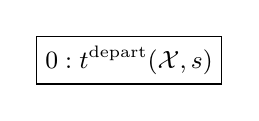
\begin{tikzpicture}
\small
\matrix[nodes={minimum size=6mm}] {
  \node[draw] {$0:t^\textrm{depart}(\mathcal{X},s)$};\\
};
\end{tikzpicture}

where $s$ is the server identified by {\Tt{}sid\nwendquote} (param. 1).\\
\textbf{Side Effects:} none.\\
\textbf{Throws:} {\Tt{}SQLException\nwendquote} if database failure is encountered.\\
\bottomrule
\end{tabular}
\nwenddocs{}\nwbegincode{145}\sublabel{NW1Dx1yV-3pEbv2-1}\nwmargintag{{\nwtagstyle{}\subpageref{NW1Dx1yV-3pEbv2-1}}}\moddef{Read: DBQueryServerTimeOfDeparture(1)~{\nwtagstyle{}\subpageref{NW1Dx1yV-3pEbv2-1}}}\endmoddef\nwstartdeflinemarkup\nwusesondefline{\\{NW46kjAM-Oyob-1}}\nwenddeflinemarkup
int[] \nwlinkedidentc{DBQueryServerTimeOfDeparture}{NW1Dx1yV-3pEbv2-1}(final int sid) throws SQLException \{
  try (\LA{}Open \code{}conn\edoc{}~{\nwtagstyle{}\subpageref{NW1ODIS0-JT1v9-1}}\RA{}) \{
    return \nwlinkedidentc{PSQuery}{NW1ODIS0-yHOIP-1}(conn, "\nwlinkedidentc{S125}{NW1ODIS0-4ds9Gt-1}", 1, sid);
  \} catch (SQLException e) \{
    throw e;
  \}
\}
\nwindexdefn{\nwixident{DBQueryServerTimeOfDeparture}}{DBQueryServerTimeOfDeparture}{NW1Dx1yV-3pEbv2-1}\eatline
\nwused{\\{NW46kjAM-Oyob-1}}\nwidentdefs{\\{{\nwixident{DBQueryServerTimeOfDeparture}}{DBQueryServerTimeOfDeparture}}}\nwidentuses{\\{{\nwixident{PSQuery}}{PSQuery}}\\{{\nwixident{S125}}{S125}}}\nwindexuse{\nwixident{PSQuery}}{PSQuery}{NW1Dx1yV-3pEbv2-1}\nwindexuse{\nwixident{S125}}{S125}{NW1Dx1yV-3pEbv2-1}\nwendcode{}\nwbegindocs{146}\begin{tabular}{p{\textwidth}}
\toprule
\rowcolor{TableTitle}
Method \textcolor{blue}{{\Tt{}\nwlinkedidentq{queryServerTimeOfDeparture}{NW1Dx1yV-3fOzh2-1}\nwendquote}}(1) wraps {\Tt{}\nwlinkedidentq{DBQueryServerTimeOfDeparture}{NW1Dx1yV-3pEbv2-1}\nwendquote}(1).\\
\bottomrule
\end{tabular}
\nwenddocs{}\nwbegincode{147}\sublabel{NW1Dx1yV-3fOzh2-1}\nwmargintag{{\nwtagstyle{}\subpageref{NW1Dx1yV-3fOzh2-1}}}\moddef{Read: queryServerTimeOfDeparture(1)~{\nwtagstyle{}\subpageref{NW1Dx1yV-3fOzh2-1}}}\endmoddef\nwstartdeflinemarkup\nwusesondefline{\\{NW3hMOhb-2u8vSA-1}}\nwenddeflinemarkup
int[] \nwlinkedidentc{queryServerTimeOfDeparture}{NW1Dx1yV-3fOzh2-1}(final int sid) throws SQLException \{
  int[] output = storage.\nwlinkedidentc{DBQueryServerTimeOfDeparture}{NW1Dx1yV-3pEbv2-1}(sid);
  return output;
\}
\nwindexdefn{\nwixident{queryServerTimeOfDeparture}}{queryServerTimeOfDeparture}{NW1Dx1yV-3fOzh2-1}\eatline
\nwused{\\{NW3hMOhb-2u8vSA-1}}\nwidentdefs{\\{{\nwixident{queryServerTimeOfDeparture}}{queryServerTimeOfDeparture}}}\nwidentuses{\\{{\nwixident{DBQueryServerTimeOfDeparture}}{DBQueryServerTimeOfDeparture}}}\nwindexuse{\nwixident{DBQueryServerTimeOfDeparture}}{DBQueryServerTimeOfDeparture}{NW1Dx1yV-3fOzh2-1}\nwendcode{}\nwbegindocs{148}\nwdocspar

\subsubsection{\texttt{DBQueryServerTimeOfArrival}(1)}
\begin{tabular}{p{\textwidth}}
\toprule
\rowcolor{TableTitle}
Method \textcolor{blue}{{\Tt{}\nwlinkedidentq{DBQueryServerTimeOfArrival}{NW1Dx1yV-4OXq2M-1}\nwendquote}}(1) returns the
arrival time $t^\textrm{arrive}(\mathcal{X},s)$
(Eq.~\ref{eq:arrival-time}) of the given server.
A {\Tt{}SQLException\nwendquote} is thrown in case of database failure.\\
\midrule
\textbf{Parameters:}\\
\begin{tabular}{lp{116mm}}
Integer {\Tt{}sid\nwendquote} (param. 1):&server identifier.
\end{tabular}\\
\textbf{Returns:} results of the query flattened into an integer array,
or {\Tt{}null\nwendquote} if no results.

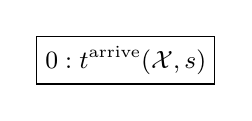
\begin{tikzpicture}
\small
\matrix[nodes={minimum size=6mm}] {
  \node[draw] {$0:t^\textrm{arrive}(\mathcal{X},s)$};\\
};
\end{tikzpicture}

where $s$ is the request identified by {\Tt{}sid\nwendquote} (param. 1).\\
\textbf{Side Effects:} none.\\
\textbf{Throws:} {\Tt{}SQLException\nwendquote} if database failure is encountered.\\
\bottomrule
\end{tabular}
\nwenddocs{}\nwbegincode{149}\sublabel{NW1Dx1yV-4OXq2M-1}\nwmargintag{{\nwtagstyle{}\subpageref{NW1Dx1yV-4OXq2M-1}}}\moddef{Read: DBQueryServerTimeOfArrival(1)~{\nwtagstyle{}\subpageref{NW1Dx1yV-4OXq2M-1}}}\endmoddef\nwstartdeflinemarkup\nwusesondefline{\\{NW46kjAM-Oyob-1}}\nwenddeflinemarkup
int[] \nwlinkedidentc{DBQueryServerTimeOfArrival}{NW1Dx1yV-4OXq2M-1}(final int sid) throws SQLException \{
  try (\LA{}Open \code{}conn\edoc{}~{\nwtagstyle{}\subpageref{NW1ODIS0-JT1v9-1}}\RA{}) \{
    return \nwlinkedidentc{PSQuery}{NW1ODIS0-yHOIP-1}(conn, "\nwlinkedidentc{S127}{NW1ODIS0-2TKHcJ-1}", 1, sid);
  \} catch (SQLException e) \{
    throw e;
  \}
\}
\nwindexdefn{\nwixident{DBQueryServerTimeOfArrival}}{DBQueryServerTimeOfArrival}{NW1Dx1yV-4OXq2M-1}\eatline
\nwused{\\{NW46kjAM-Oyob-1}}\nwidentdefs{\\{{\nwixident{DBQueryServerTimeOfArrival}}{DBQueryServerTimeOfArrival}}}\nwidentuses{\\{{\nwixident{PSQuery}}{PSQuery}}\\{{\nwixident{S127}}{S127}}}\nwindexuse{\nwixident{PSQuery}}{PSQuery}{NW1Dx1yV-4OXq2M-1}\nwindexuse{\nwixident{S127}}{S127}{NW1Dx1yV-4OXq2M-1}\nwendcode{}\nwbegindocs{150}\begin{tabular}{p{\textwidth}}
\toprule
\rowcolor{TableTitle}
Method \textcolor{blue}{{\Tt{}\nwlinkedidentq{queryServerTimeOfArrival}{NW1Dx1yV-3Rabqu-1}\nwendquote}}(1) wraps {\Tt{}\nwlinkedidentq{DBQueryServerTimeOfArrival}{NW1Dx1yV-4OXq2M-1}\nwendquote}(1).\\
\bottomrule
\end{tabular}
\nwenddocs{}\nwbegincode{151}\sublabel{NW1Dx1yV-3Rabqu-1}\nwmargintag{{\nwtagstyle{}\subpageref{NW1Dx1yV-3Rabqu-1}}}\moddef{Read: queryServerTimeOfArrival(1)~{\nwtagstyle{}\subpageref{NW1Dx1yV-3Rabqu-1}}}\endmoddef\nwstartdeflinemarkup\nwenddeflinemarkup
int[] \nwlinkedidentc{queryServerTimeOfArrival}{NW1Dx1yV-3Rabqu-1}(final int sid) throws SQLException \{
  int[] output = storage.\nwlinkedidentc{DBQueryServerTimeOfArrival}{NW1Dx1yV-4OXq2M-1}(sid);
  return output;
\}
\nwindexdefn{\nwixident{queryServerTimeOfArrival}}{queryServerTimeOfArrival}{NW1Dx1yV-3Rabqu-1}\eatline
\nwnotused{Read: queryServerTimeOfArrival(1)}\nwidentdefs{\\{{\nwixident{queryServerTimeOfArrival}}{queryServerTimeOfArrival}}}\nwidentuses{\\{{\nwixident{DBQueryServerTimeOfArrival}}{DBQueryServerTimeOfArrival}}}\nwindexuse{\nwixident{DBQueryServerTimeOfArrival}}{DBQueryServerTimeOfArrival}{NW1Dx1yV-3Rabqu-1}\nwendcode{}\nwbegindocs{152}\nwdocspar
\subsubsection{\texttt{DBQueryServerAssignmentsPending}(2)}
\begin{tabular}{p{\textwidth}}
\toprule
\rowcolor{TableTitle}
Method \textcolor{blue}{{\Tt{}\nwlinkedidentq{DBQueryServerAssignmentsPending}{NW1Dx1yV-2nZ1VB-1}\nwendquote}}(2) returns the
requests that will be picked up by the given server beyond the given time.
A {\Tt{}SQLException\nwendquote} is thrown in case of database failure.\\
\midrule
\textbf{Parameters:} \\
\begin{tabular}{lp{116mm}}
Integer {\Tt{}sid\nwendquote} (param. 1):&server identifier.\\
Integer {\Tt{}t\nwendquote} (param. 2):&a time.\\
\end{tabular}
\textbf{Returns:} results of the query flattened into an integer array,
or {\Tt{}null\nwendquote} if no results.

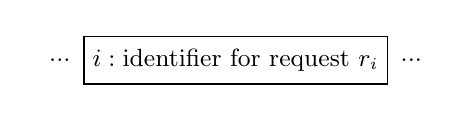
\begin{tikzpicture}
\small
\matrix[nodes={minimum size=6mm}] {
  \node {...};
 &\node[draw] {$i:\textrm{identifier for request }r_i$};
 &\node {...};\\
};
\end{tikzpicture}

where $1\leq i\leq |R^\textrm{pending}(\mathcal{X}, s, t)|$,
$r_i\in R^\textrm{pending}(\mathcal{X}, s, t)$, and
$R^\textrm{pending}(\mathcal{X}, s, t)= (R(\mathcal{X},s,H)\setminus R(\mathcal{X},s,t))$ for
time horizon $H$, server $s$ identified by {\Tt{}sid\nwendquote} (param. 1), and time $t$ given by param. 2.\\
\textbf{Side Effects:} none.\\
\textbf{Throws:} {\Tt{}SQLException\nwendquote} if database failure is encountered.\\
\bottomrule
\end{tabular}
\nwenddocs{}\nwbegincode{153}\sublabel{NW1Dx1yV-2nZ1VB-1}\nwmargintag{{\nwtagstyle{}\subpageref{NW1Dx1yV-2nZ1VB-1}}}\moddef{Read: DBQueryServerAssignmentsPending(2)~{\nwtagstyle{}\subpageref{NW1Dx1yV-2nZ1VB-1}}}\endmoddef\nwstartdeflinemarkup\nwusesondefline{\\{NW46kjAM-Oyob-1}}\nwenddeflinemarkup
int[] \nwlinkedidentc{DBQueryServerAssignmentsPending}{NW1Dx1yV-2nZ1VB-1}(final int sid, final int t)
throws SQLException \{
  try (\LA{}Open \code{}conn\edoc{}~{\nwtagstyle{}\subpageref{NW1ODIS0-JT1v9-1}}\RA{}) \{
    return \nwlinkedidentc{PSQuery}{NW1ODIS0-yHOIP-1}(conn, "\nwlinkedidentc{S100}{NW1ODIS0-yxMXz-1}", 1, t, sid);
  \} catch (SQLException e) \{
    throw e;
  \}
\}
\nwindexdefn{\nwixident{DBQueryServerAssignmentsPending}}{DBQueryServerAssignmentsPending}{NW1Dx1yV-2nZ1VB-1}\eatline
\nwused{\\{NW46kjAM-Oyob-1}}\nwidentdefs{\\{{\nwixident{DBQueryServerAssignmentsPending}}{DBQueryServerAssignmentsPending}}}\nwidentuses{\\{{\nwixident{PSQuery}}{PSQuery}}\\{{\nwixident{S100}}{S100}}}\nwindexuse{\nwixident{PSQuery}}{PSQuery}{NW1Dx1yV-2nZ1VB-1}\nwindexuse{\nwixident{S100}}{S100}{NW1Dx1yV-2nZ1VB-1}\nwendcode{}\nwbegindocs{154}\nwdocspar
\subsubsection{\texttt{DBQueryServerAssignmentsCompleted}(2)}
\begin{tabular}{p{\textwidth}}
\toprule
\rowcolor{TableTitle}
Method \textcolor{blue}{{\Tt{}\nwlinkedidentq{DBQueryServerAssignmentsCompleted}{NW1Dx1yV-31osvi-1}\nwendquote}}(2) returns the
requests that have been dropped off by the given server on or before the given time,
in other words $R(\mathcal{X},s,t)$ (Eq.~\ref{eq:R(X,s,t)}).
A {\Tt{}SQLException\nwendquote} is thrown in case of database failure.\\
\midrule
\textbf{Parameters:} \\
\begin{tabular}{lp{116mm}}
Integer {\Tt{}sid\nwendquote} (param. 1):&server identifier.\\
Integer {\Tt{}t\nwendquote} (param. 2):&a time.\\
\end{tabular}
\textbf{Returns:} results of the query flattened into an integer array,
or {\Tt{}null\nwendquote} if no results.

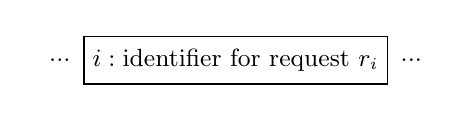
\begin{tikzpicture}
\small
\matrix[nodes={minimum size=6mm}] {
  \node {...};
 &\node[draw] {$i:\textrm{identifier for request }r_i$};
 &\node {...};\\
};
\end{tikzpicture}

where $1\leq i\leq |R(\mathcal{X},s,t)|$ and
$r_i\in R(\mathcal{X},s,t)$ for server $s$ identified by {\Tt{}sid\nwendquote} (param. 1)
at time $t$ given by param. 2.\\
\textbf{Side Effects:} none.\\
\textbf{Throws:} {\Tt{}SQLException\nwendquote} if database failure is encountered.\\
\bottomrule
\end{tabular}
\nwenddocs{}\nwbegincode{155}\sublabel{NW1Dx1yV-31osvi-1}\nwmargintag{{\nwtagstyle{}\subpageref{NW1Dx1yV-31osvi-1}}}\moddef{Read: DBQueryServerAssignmentsCompleted(2)~{\nwtagstyle{}\subpageref{NW1Dx1yV-31osvi-1}}}\endmoddef\nwstartdeflinemarkup\nwusesondefline{\\{NW46kjAM-Oyob-1}}\nwenddeflinemarkup
int[] \nwlinkedidentc{DBQueryServerAssignmentsCompleted}{NW1Dx1yV-31osvi-1}(final int sid, final int t)
throws SQLException \{
  try (\LA{}Open \code{}conn\edoc{}~{\nwtagstyle{}\subpageref{NW1ODIS0-JT1v9-1}}\RA{}) \{
    return \nwlinkedidentc{PSQuery}{NW1ODIS0-yHOIP-1}(conn, "\nwlinkedidentc{S101}{NW1ODIS0-3WmKrr-1}", 1, t, sid);
  \} catch (SQLException e) \{
    throw e;
  \}
\}
\nwindexdefn{\nwixident{DBQueryServerAssignmentsCompleted}}{DBQueryServerAssignmentsCompleted}{NW1Dx1yV-31osvi-1}\eatline
\nwused{\\{NW46kjAM-Oyob-1}}\nwidentdefs{\\{{\nwixident{DBQueryServerAssignmentsCompleted}}{DBQueryServerAssignmentsCompleted}}}\nwidentuses{\\{{\nwixident{PSQuery}}{PSQuery}}\\{{\nwixident{S101}}{S101}}}\nwindexuse{\nwixident{PSQuery}}{PSQuery}{NW1Dx1yV-31osvi-1}\nwindexuse{\nwixident{S101}}{S101}{NW1Dx1yV-31osvi-1}\nwendcode{}\nwbegindocs{156}\nwdocspar
\subsubsection{\texttt{DBQueryServersActive}(1)}
\begin{tabular}{p{\textwidth}}
\toprule
\rowcolor{TableTitle}
Method \textcolor{blue}{{\Tt{}\nwlinkedidentq{DBQueryServersActive}{NW1Dx1yV-3NWzRo-1}\nwendquote}}(1) returns the identifiers
of the active servers at the given time. A server is ``active'' if its
service has not ended.
A {\Tt{}SQLException\nwendquote} is thrown in case of database failure.\\
\midrule
\textbf{Parameters:} \\
\begin{tabular}{lp{116mm}}
Integer {\Tt{}t\nwendquote} (param. 1):&a time
\end{tabular}\\
\textbf{Returns:} results of the query flattened into an integer array, or
{\Tt{}null\nwendquote} if no results.

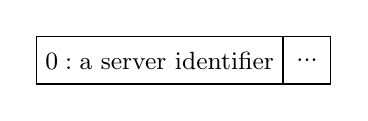
\begin{tikzpicture}
\small
\matrix[nodes={draw,minimum size=6mm}] {
  \node {$0:\textrm{a server identifier}$};
 &\node {...};\\
};
\end{tikzpicture}\\
\textbf{Side Effects:} none.\\
\textbf{Throws:} {\Tt{}SQLException\nwendquote} if database failure is encountered.\\
\bottomrule
\end{tabular}
\nwenddocs{}\nwbegincode{157}\sublabel{NW1Dx1yV-3NWzRo-1}\nwmargintag{{\nwtagstyle{}\subpageref{NW1Dx1yV-3NWzRo-1}}}\moddef{Read: DBQueryServersActive(1)~{\nwtagstyle{}\subpageref{NW1Dx1yV-3NWzRo-1}}}\endmoddef\nwstartdeflinemarkup\nwusesondefline{\\{NW46kjAM-Oyob-1}}\nwenddeflinemarkup
int[] \nwlinkedidentc{DBQueryServersActive}{NW1Dx1yV-3NWzRo-1}(final int t) throws SQLException \{
  try (\LA{}Open \code{}conn\edoc{}~{\nwtagstyle{}\subpageref{NW1ODIS0-JT1v9-1}}\RA{}) \{
    return this.\nwlinkedidentc{PSQuery}{NW1ODIS0-yHOIP-1}(conn, "\nwlinkedidentc{S134}{NW1ODIS0-9eEGJ-1}", 1, t, t, t);
  \} catch (SQLException e) \{
    throw e;
  \}
\}
\nwindexdefn{\nwixident{DBQueryServersActive}}{DBQueryServersActive}{NW1Dx1yV-3NWzRo-1}\eatline
\nwused{\\{NW46kjAM-Oyob-1}}\nwidentdefs{\\{{\nwixident{DBQueryServersActive}}{DBQueryServersActive}}}\nwidentuses{\\{{\nwixident{PSQuery}}{PSQuery}}\\{{\nwixident{S134}}{S134}}}\nwindexuse{\nwixident{PSQuery}}{PSQuery}{NW1Dx1yV-3NWzRo-1}\nwindexuse{\nwixident{S134}}{S134}{NW1Dx1yV-3NWzRo-1}\nwendcode{}\nwbegincode{158}\sublabel{NW1Dx1yV-4USAYN-1}\nwmargintag{{\nwtagstyle{}\subpageref{NW1Dx1yV-4USAYN-1}}}\moddef{Read: queryServersActive(1)~{\nwtagstyle{}\subpageref{NW1Dx1yV-4USAYN-1}}}\endmoddef\nwstartdeflinemarkup\nwusesondefline{\\{NW3hMOhb-2u8vSA-1}}\nwenddeflinemarkup
int[] \nwlinkedidentc{queryServersActive}{NW1Dx1yV-4USAYN-1}(final int t) throws SQLException \{
  int[] output = this.storage.\nwlinkedidentc{DBQueryServersActive}{NW1Dx1yV-3NWzRo-1}(t);
  return output;
\}
\nwindexdefn{\nwixident{queryServersActive}}{queryServersActive}{NW1Dx1yV-4USAYN-1}\eatline
\nwused{\\{NW3hMOhb-2u8vSA-1}}\nwidentdefs{\\{{\nwixident{queryServersActive}}{queryServersActive}}}\nwidentuses{\\{{\nwixident{DBQueryServersActive}}{DBQueryServersActive}}}\nwindexuse{\nwixident{DBQueryServersActive}}{DBQueryServersActive}{NW1Dx1yV-4USAYN-1}\nwendcode{}\nwbegindocs{159}\nwdocspar
\subsubsection{\texttt{DBQueryServersCount}(0)}
\begin{tabular}{p{\textwidth}}
\toprule
\rowcolor{TableTitle}
Method \textcolor{blue}{{\Tt{}DBQueryCountSevers\nwendquote}}(0) returns the total number
of servers in Table S.
A {\Tt{}SQLException\nwendquote} is thrown in case of database failure.\\
\midrule
\textbf{Parameters:} none.\\
\textbf{Returns:} results of the query flattened into an integer array, or
{\Tt{}null\nwendquote} if no results.

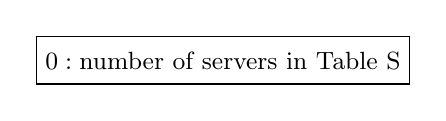
\begin{tikzpicture}
\small
\matrix[nodes={draw,minimum size=6mm}] {
  \node {$0:\textrm{number of servers in Table S}$};\\
};
\end{tikzpicture}\\
\textbf{Side Effects:} none.\\
\textbf{Throws:} {\Tt{}SQLException\nwendquote} if database failure is encountered.\\
\bottomrule
\end{tabular}
\nwenddocs{}\nwbegincode{160}\sublabel{NW1Dx1yV-23ZhQ2-1}\nwmargintag{{\nwtagstyle{}\subpageref{NW1Dx1yV-23ZhQ2-1}}}\moddef{Read: DBQueryServersCount(0)~{\nwtagstyle{}\subpageref{NW1Dx1yV-23ZhQ2-1}}}\endmoddef\nwstartdeflinemarkup\nwusesondefline{\\{NW46kjAM-Oyob-1}}\nwenddeflinemarkup
int[] \nwlinkedidentc{DBQueryServersCount}{NW1Dx1yV-23ZhQ2-1}() throws SQLException \{
  try (\LA{}Open \code{}conn\edoc{}~{\nwtagstyle{}\subpageref{NW1ODIS0-JT1v9-1}}\RA{}) \{
    return this.\nwlinkedidentc{PSQuery}{NW1ODIS0-yHOIP-1}(conn, "\nwlinkedidentc{S66}{NW1ODIS0-1SEANQ-1}", 1);
  \} catch (SQLException e) \{
    throw e;
  \}
\}
\nwindexdefn{\nwixident{DBQueryServersCount}}{DBQueryServersCount}{NW1Dx1yV-23ZhQ2-1}\eatline
\nwused{\\{NW46kjAM-Oyob-1}}\nwidentdefs{\\{{\nwixident{DBQueryServersCount}}{DBQueryServersCount}}}\nwidentuses{\\{{\nwixident{PSQuery}}{PSQuery}}\\{{\nwixident{S66}}{S66}}}\nwindexuse{\nwixident{PSQuery}}{PSQuery}{NW1Dx1yV-23ZhQ2-1}\nwindexuse{\nwixident{S66}}{S66}{NW1Dx1yV-23ZhQ2-1}\nwendcode{}\nwbegindocs{161}\begin{tabular}{p{\textwidth}}
\toprule
\rowcolor{TableTitle}
Method \textcolor{blue}{{\Tt{}\nwlinkedidentq{queryServersCount}{NW1Dx1yV-3YlcHc-1}\nwendquote}}(0) wraps {\Tt{}\nwlinkedidentq{DBQueryServersCount}{NW1Dx1yV-23ZhQ2-1}\nwendquote}(0).\\
\bottomrule
\end{tabular}
\nwenddocs{}\nwbegincode{162}\sublabel{NW1Dx1yV-3YlcHc-1}\nwmargintag{{\nwtagstyle{}\subpageref{NW1Dx1yV-3YlcHc-1}}}\moddef{Read: queryServersCount(0)~{\nwtagstyle{}\subpageref{NW1Dx1yV-3YlcHc-1}}}\endmoddef\nwstartdeflinemarkup\nwusesondefline{\\{NW3hMOhb-2u8vSA-1}}\nwenddeflinemarkup
int[] \nwlinkedidentc{queryServersCount}{NW1Dx1yV-3YlcHc-1}() throws SQLException \{
  int[] output = storage.\nwlinkedidentc{DBQueryServersCount}{NW1Dx1yV-23ZhQ2-1}();
  return output;
\}
\nwindexdefn{\nwixident{queryServersCount}}{queryServersCount}{NW1Dx1yV-3YlcHc-1}\eatline
\nwused{\\{NW3hMOhb-2u8vSA-1}}\nwidentdefs{\\{{\nwixident{queryServersCount}}{queryServersCount}}}\nwidentuses{\\{{\nwixident{DBQueryServersCount}}{DBQueryServersCount}}}\nwindexuse{\nwixident{DBQueryServersCount}}{DBQueryServersCount}{NW1Dx1yV-3YlcHc-1}\nwendcode{}\nwbegindocs{163}\nwdocspar
\subsubsection{\texttt{DBQueryServersCountActive}(1)}
\begin{tabular}{p{\textwidth}}
\toprule
\rowcolor{TableTitle}
Method \textcolor{blue}{{\Tt{}\nwlinkedidentq{DBQueryServersCountActive}{NW1Dx1yV-1014SS-1}\nwendquote}}(1) returns the identifiers
of the active servers at the given time. A server is ``active'' if its
service has not ended.
A {\Tt{}SQLException\nwendquote} is thrown in case of database failure.\\
\midrule
\textbf{Parameters:} \\
\begin{tabular}{lp{116mm}}
Integer {\Tt{}t\nwendquote} (param. 1):&a time
\end{tabular}\\
\textbf{Returns:} results of the query flattened into an integer array, or
{\Tt{}null\nwendquote} if no results.

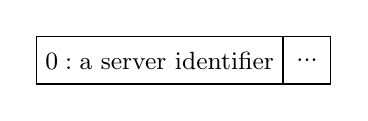
\begin{tikzpicture}
\small
\matrix[nodes={draw,minimum size=6mm}] {
  \node {$0:\textrm{a server identifier}$};
 &\node {...};\\
};
\end{tikzpicture}\\
\textbf{Side Effects:} none.\\
\textbf{Throws:} {\Tt{}SQLException\nwendquote} if database failure is encountered.\\
\bottomrule
\end{tabular}
\nwenddocs{}\nwbegincode{164}\sublabel{NW1Dx1yV-1014SS-1}\nwmargintag{{\nwtagstyle{}\subpageref{NW1Dx1yV-1014SS-1}}}\moddef{Read: DBQueryServersCountActive(1)~{\nwtagstyle{}\subpageref{NW1Dx1yV-1014SS-1}}}\endmoddef\nwstartdeflinemarkup\nwusesondefline{\\{NW46kjAM-Oyob-1}}\nwenddeflinemarkup
int[] \nwlinkedidentc{DBQueryServersCountActive}{NW1Dx1yV-1014SS-1}(final int t) throws SQLException \{
  try (\LA{}Open \code{}conn\edoc{}~{\nwtagstyle{}\subpageref{NW1ODIS0-JT1v9-1}}\RA{}) \{
    return new int[] \{ this.\nwlinkedidentc{PSQuery}{NW1ODIS0-yHOIP-1}(conn, "\nwlinkedidentc{S134}{NW1ODIS0-9eEGJ-1}", 1, t, t, t).length/2 \};
  \} catch (SQLException e) \{
    throw e;
  \}
\}
\nwindexdefn{\nwixident{DBQueryServersCountActive}}{DBQueryServersCountActive}{NW1Dx1yV-1014SS-1}\eatline
\nwused{\\{NW46kjAM-Oyob-1}}\nwidentdefs{\\{{\nwixident{DBQueryServersCountActive}}{DBQueryServersCountActive}}}\nwidentuses{\\{{\nwixident{PSQuery}}{PSQuery}}\\{{\nwixident{S134}}{S134}}}\nwindexuse{\nwixident{PSQuery}}{PSQuery}{NW1Dx1yV-1014SS-1}\nwindexuse{\nwixident{S134}}{S134}{NW1Dx1yV-1014SS-1}\nwendcode{}\nwbegincode{165}\sublabel{NW1Dx1yV-3m8NX0-1}\nwmargintag{{\nwtagstyle{}\subpageref{NW1Dx1yV-3m8NX0-1}}}\moddef{Read: queryServersCountActive(1)~{\nwtagstyle{}\subpageref{NW1Dx1yV-3m8NX0-1}}}\endmoddef\nwstartdeflinemarkup\nwusesondefline{\\{NW3hMOhb-2u8vSA-1}}\nwenddeflinemarkup
int[] \nwlinkedidentc{queryServersCountActive}{NW1Dx1yV-3m8NX0-1}(final int t) throws SQLException \{
  int[] output = this.storage.\nwlinkedidentc{DBQueryServersCountActive}{NW1Dx1yV-1014SS-1}(t);
  return output;
\}
\nwindexdefn{\nwixident{queryServersCountActive}}{queryServersCountActive}{NW1Dx1yV-3m8NX0-1}\eatline
\nwused{\\{NW3hMOhb-2u8vSA-1}}\nwidentdefs{\\{{\nwixident{queryServersCountActive}}{queryServersCountActive}}}\nwidentuses{\\{{\nwixident{DBQueryServersCountActive}}{DBQueryServersCountActive}}}\nwindexuse{\nwixident{DBQueryServersCountActive}}{DBQueryServersCountActive}{NW1Dx1yV-3m8NX0-1}\nwendcode{}\nwbegindocs{166}\nwdocspar
\subsubsection{\texttt{DBQueryServersCountAppeared}(0)}
TODO. Very bad method name. A server counts as "appeared" only if its route
distance is greater than 0. For example, a taxi that is idling and has never
moved does not count as "appeared".
\nwenddocs{}\nwbegincode{167}\sublabel{NW1Dx1yV-w1r5F-1}\nwmargintag{{\nwtagstyle{}\subpageref{NW1Dx1yV-w1r5F-1}}}\moddef{Read: DBQueryServersCountAppeared(0)~{\nwtagstyle{}\subpageref{NW1Dx1yV-w1r5F-1}}}\endmoddef\nwstartdeflinemarkup\nwenddeflinemarkup
int[] \nwlinkedidentc{DBQueryServersCountAppeared}{NW1Dx1yV-w1r5F-1}() throws SQLException \{
  int[] output = new int[] \{ \};
  // ...
  return output;
\}
\nwindexdefn{\nwixident{DBQueryServersCountAppeared}}{DBQueryServersCountAppeared}{NW1Dx1yV-w1r5F-1}\eatline
\nwnotused{Read: DBQueryServersCountAppeared(0)}\nwidentdefs{\\{{\nwixident{DBQueryServersCountAppeared}}{DBQueryServersCountAppeared}}}\nwendcode{}\nwbegincode{168}\sublabel{NW1Dx1yV-1u7qwL-1}\nwmargintag{{\nwtagstyle{}\subpageref{NW1Dx1yV-1u7qwL-1}}}\moddef{Read: queryServersCountAppeared(0)~{\nwtagstyle{}\subpageref{NW1Dx1yV-1u7qwL-1}}}\endmoddef\nwstartdeflinemarkup\nwusesondefline{\\{NW3hMOhb-2u8vSA-1}}\nwenddeflinemarkup
int[] \nwlinkedidentc{queryServersCountAppeared}{NW1Dx1yV-1u7qwL-1}() throws SQLException \{
  int[] output = new int[] \{ 0 \};
  for (int sid : this.lu_sseen.keySet()) \{
    if (this.storage.\nwlinkedidentc{DBQueryServerDistance}{NW1Dx1yV-bdI1v-1}(sid, true)[0] > 0) \{
      output[0]++;
    \}
  \}
  return output;
\}
\nwindexdefn{\nwixident{queryServersCountAppeared}}{queryServersCountAppeared}{NW1Dx1yV-1u7qwL-1}\eatline
\nwused{\\{NW3hMOhb-2u8vSA-1}}\nwidentdefs{\\{{\nwixident{queryServersCountAppeared}}{queryServersCountAppeared}}}\nwidentuses{\\{{\nwixident{DBQueryServerDistance}}{DBQueryServerDistance}}}\nwindexuse{\nwixident{DBQueryServerDistance}}{DBQueryServerDistance}{NW1Dx1yV-1u7qwL-1}\nwendcode{}\nwbegindocs{169}\subsubsection{\texttt{DBQueryServersLocations}(1)}
\begin{tabular}{p{\textwidth}}
\toprule
\rowcolor{TableTitle}
Method \textcolor{blue}{{\Tt{}\nwlinkedidentq{DBQueryServersLocations}{NW1Dx1yV-1zUdrf-1}\nwendquote}}(1) returns the
last-known locations of all servers (including inactive servers) at the given
time. The ``last-known location'' is the waypoint in the server's route $w$
with a time component closest to but not exceeding the given time, in other
words ${w_{\leq t}}_{|w_{\leq t}|}$.
A {\Tt{}SQLException\nwendquote} is thrown in case of database failure.\\
\midrule
\textbf{Parameters:} \\
\begin{tabular}{lp{116mm}}
Integer {\Tt{}t\nwendquote} (param. 1):&a time
\end{tabular}\\
\textbf{Returns:} results of the query flattened into an integer array, or
{\Tt{}null\nwendquote} if no results.

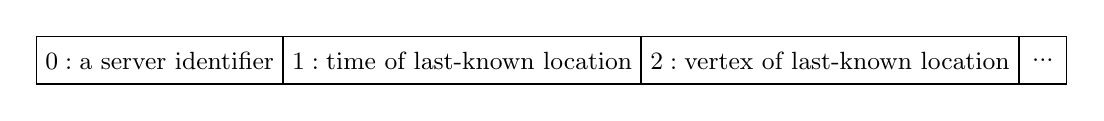
\begin{tikzpicture}
\small
\matrix[nodes={draw,minimum size=6mm}] {
  \node {$0:\textrm{a server identifier}$};
 &\node {$1:\textrm{time of last-known location}$};
 &\node {$2:\textrm{vertex of last-known location}$};
 &\node {...};\\
};
\end{tikzpicture}\\
\textbf{Side Effects:} none.\\
\textbf{Throws:} {\Tt{}SQLException\nwendquote} if database failure is encountered.\\
\bottomrule
\end{tabular}
\nwenddocs{}\nwbegincode{170}\sublabel{NW1Dx1yV-1zUdrf-1}\nwmargintag{{\nwtagstyle{}\subpageref{NW1Dx1yV-1zUdrf-1}}}\moddef{Read: DBQueryServersLocations(1)~{\nwtagstyle{}\subpageref{NW1Dx1yV-1zUdrf-1}}}\endmoddef\nwstartdeflinemarkup\nwusesondefline{\\{NW46kjAM-Oyob-1}}\nwenddeflinemarkup
int[] \nwlinkedidentc{DBQueryServersLocations}{NW1Dx1yV-1zUdrf-1}(final int t) throws SQLException \{
  try (\LA{}Open \code{}conn\edoc{}~{\nwtagstyle{}\subpageref{NW1ODIS0-JT1v9-1}}\RA{}) \{
    return this.\nwlinkedidentc{PSQuery}{NW1ODIS0-yHOIP-1}(conn, "\nwlinkedidentc{S59}{NW1ODIS0-4APdTA-1}", 3, t, t, t, t);
  \} catch (SQLException e) \{
    throw e;
  \}
\}
\nwindexdefn{\nwixident{DBQueryServersLocations}}{DBQueryServersLocations}{NW1Dx1yV-1zUdrf-1}\eatline
\nwused{\\{NW46kjAM-Oyob-1}}\nwidentdefs{\\{{\nwixident{DBQueryServersLocations}}{DBQueryServersLocations}}}\nwidentuses{\\{{\nwixident{PSQuery}}{PSQuery}}\\{{\nwixident{S59}}{S59}}}\nwindexuse{\nwixident{PSQuery}}{PSQuery}{NW1Dx1yV-1zUdrf-1}\nwindexuse{\nwixident{S59}}{S59}{NW1Dx1yV-1zUdrf-1}\nwendcode{}\nwbegindocs{171}\nwdocspar
\subsubsection{\texttt{DBQueryServersLocationsActive}(1)}
\begin{tabular}{p{\textwidth}}
\toprule
\rowcolor{TableTitle}
SINGLE-THREAD ONLY. Method \textcolor{blue}{{\Tt{}\nwlinkedidentq{DBQueryServersLocationsActive}{NW1Dx1yV-2tWQc-1}\nwendquote}}(1) returns the
last-known locations of all active servers at the given time. A server is
``active'' if its service has not ended, in other words it has not arrived
at its own destination.
The ``last-known location'' is the waypoint in the server's route $w$
with a time component closest to but not exceeding the given time, in other
words ${w_{\leq t}}_{|w_{\leq t}|}$.
A {\Tt{}SQLException\nwendquote} is thrown in case of database failure.\\
\midrule
\textbf{Parameters:} \\
\begin{tabular}{lp{116mm}}
Integer {\Tt{}t\nwendquote} (param. 1):&a time
\end{tabular}\\
\textbf{Returns:} results of the query flattened into an integer array, or
{\Tt{}null\nwendquote} if no results.

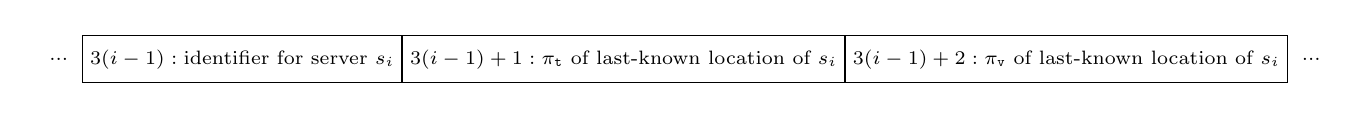
\begin{tikzpicture}
\scriptsize
\matrix[nodes={minimum size=6mm}] {
  \node {...};
 &\node[draw] {$3(i-1):\textrm{identifier for server $s_i$}$};
 &\node[draw] {$3(i-1)+1:\pi_\texttt{t}\textrm{ of last-known location of $s_i$}$};
 &\node[draw] {$3(i-1)+2:\pi_\texttt{v}\textrm{ of last-known location of $s_i$}$};
 &\node {...};\\
};
\end{tikzpicture}\\

where $1\leq i\leq |\mathcal{S}^\textrm{active}|$,
$s_i\in \mathcal{S}^\textrm{active}$, and
$\mathcal{S}^\textrm{active}= \{s\in\mathcal{S}\mid t^\textrm{arrive}(\mathcal{X},s)>t\}|$
for $t$ given by param. 1.\\
\textbf{Side Effects:} none.\\
\textbf{Throws:} {\Tt{}SQLException\nwendquote} if database failure is encountered.\\
\bottomrule
\end{tabular}
\nwenddocs{}\nwbegincode{172}\sublabel{NW1Dx1yV-2tWQc-1}\nwmargintag{{\nwtagstyle{}\subpageref{NW1Dx1yV-2tWQc-1}}}\moddef{Read: DBQueryServersLocationsActive(1)~{\nwtagstyle{}\subpageref{NW1Dx1yV-2tWQc-1}}}\endmoddef\nwstartdeflinemarkup\nwusesondefline{\\{NW46kjAM-Oyob-1}}\nwprevnextdefs{\relax}{NW1Dx1yV-2tWQc-2}\nwenddeflinemarkup
int[] \nwlinkedidentc{DBQueryServersLocationsActive}{NW1Dx1yV-2tWQc-1}(final int t) throws SQLException \{
  int[] output = new int[] \{ \};
  try (\LA{}Open \code{}conn\edoc{}~{\nwtagstyle{}\subpageref{NW1ODIS0-JT1v9-1}}\RA{}) \{
    int j = 0;
\nwindexdefn{\nwixident{DBQueryServersLocationsActive}}{DBQueryServersLocationsActive}{NW1Dx1yV-2tWQc-1}\eatline
\nwalsodefined{\\{NW1Dx1yV-2tWQc-2}}\nwused{\\{NW46kjAM-Oyob-1}}\nwidentdefs{\\{{\nwixident{DBQueryServersLocationsActive}}{DBQueryServersLocationsActive}}}\nwendcode{}\nwbegindocs{173}{\small Our approach is to first use statement {\Tt{}\nwlinkedidentq{S134}{NW1ODIS0-9eEGJ-1}\nwendquote} to get the active
servers. Then for each active server, we use either statement {\Tt{}\nwlinkedidentq{S135}{NW1ODIS0-4dp7jX-1}\nwendquote} or
{\Tt{}\nwlinkedidentq{S147}{NW1ODIS0-2TcddD-1}\nwendquote} to get its last-known location.}
\nwenddocs{}\nwbegincode{174}\sublabel{NW1Dx1yV-2tWQc-2}\nwmargintag{{\nwtagstyle{}\subpageref{NW1Dx1yV-2tWQc-2}}}\moddef{Read: DBQueryServersLocationsActive(1)~{\nwtagstyle{}\subpageref{NW1Dx1yV-2tWQc-1}}}\plusendmoddef\nwstartdeflinemarkup\nwusesondefline{\\{NW46kjAM-Oyob-1}}\nwprevnextdefs{NW1Dx1yV-2tWQc-1}{\relax}\nwenddeflinemarkup
    // Query \nwlinkedidentc{S134}{NW1ODIS0-9eEGJ-1} selects from CW. The \nwlinkedidentc{query}{NW1Dx1yV-47dtTX-1} time is not expected to grow
    // because Table CW does not grow as we pre-load all the servers when we
    // load the problem instance.
    final int[] temp1 = this.\nwlinkedidentc{PSQuery}{NW1ODIS0-yHOIP-1}(conn, "\nwlinkedidentc{S134}{NW1ODIS0-9eEGJ-1}", 2, t, t, t);  // <-- 10 ms/call
    output = new int[(3*(temp1.length/2))];
    for (int i = 0; i < temp1.length - 1; i += 2) \{
      final int sid = temp1[(i + 0)];
      final int  te = temp1[(i + 1)];
      // Query \nwlinkedidentc{S135}{NW1ODIS0-4dp7jX-1} selects from W. The \nwlinkedidentc{query}{NW1Dx1yV-47dtTX-1} time is expected to grow
      // O(log(|W|)) because we have indexes on the relevant columns,
      // implemented in Derby as B+trees (https://db.apache.org/derby/papers/btree_package.html).
      // The subquery in \nwlinkedidentc{S135}{NW1ODIS0-4dp7jX-1} is a range \nwlinkedidentc{query}{NW1Dx1yV-47dtTX-1} with a tight range.
      // Query \nwlinkedidentc{S147}{NW1ODIS0-2TcddD-1} is a key-lookup and also grows O(log(|W|)).
      final int lvt = this.lu_lvt.get(sid);
      final int[] temp2 = (t < te
        ? this.\nwlinkedidentc{PSQuery}{NW1ODIS0-yHOIP-1}(conn, "\nwlinkedidentc{S135}{NW1ODIS0-4dp7jX-1}", 2, sid, sid, lvt, t, t)
        : this.\nwlinkedidentc{PSQuery}{NW1ODIS0-yHOIP-1}(conn, "\nwlinkedidentc{S147}{NW1ODIS0-2TcddD-1}", 2, sid, sid));
      output[(j + 0)] = sid;
      if (temp2.length == 0) \{
        // Means server hasn't left origin yet, we just get se, so
        int[] temp3 = \nwlinkedidentc{DBQueryUser}{NW1Dx1yV-8IJdE-1}(sid);
        output[(j + 1)] = temp3[2];
        output[(j + 2)] = temp3[4];
        this.lu_lvt.put(sid, t);
      \} else \{
        output[(j + 1)] = temp2[0];
        output[(j + 2)] = temp2[1];
        this.lu_lvt.put(sid, temp2[0]);
      \}
      j += 3;
    \}
  \} catch (SQLException e) \{
    throw e;
  \} catch (\nwlinkedidentc{UserNotFoundException}{NW1ODIS0-15irq2-1} e) \{
    // Should never happen
    System.err.println("Fatal error: "+e.toString());
    System.exit(1);
  \}
  return output;
\}
\nwused{\\{NW46kjAM-Oyob-1}}\nwidentuses{\\{{\nwixident{DBQueryUser}}{DBQueryUser}}\\{{\nwixident{PSQuery}}{PSQuery}}\\{{\nwixident{query}}{query}}\\{{\nwixident{S134}}{S134}}\\{{\nwixident{S135}}{S135}}\\{{\nwixident{S147}}{S147}}\\{{\nwixident{UserNotFoundException}}{UserNotFoundException}}}\nwindexuse{\nwixident{DBQueryUser}}{DBQueryUser}{NW1Dx1yV-2tWQc-2}\nwindexuse{\nwixident{PSQuery}}{PSQuery}{NW1Dx1yV-2tWQc-2}\nwindexuse{\nwixident{query}}{query}{NW1Dx1yV-2tWQc-2}\nwindexuse{\nwixident{S134}}{S134}{NW1Dx1yV-2tWQc-2}\nwindexuse{\nwixident{S135}}{S135}{NW1Dx1yV-2tWQc-2}\nwindexuse{\nwixident{S147}}{S147}{NW1Dx1yV-2tWQc-2}\nwindexuse{\nwixident{UserNotFoundException}}{UserNotFoundException}{NW1Dx1yV-2tWQc-2}\nwendcode{}\nwbegindocs{175}\nwdocspar
\begin{tabular}{p{\textwidth}}
\toprule
\rowcolor{TableTitle}
Method \textcolor{blue}{{\Tt{}\nwlinkedidentq{queryServersLocationsActive}{NW1Dx1yV-t5O2a-1}\nwendquote}}(1) wraps {\Tt{}\nwlinkedidentq{DBQueryServersLocationsActive}{NW1Dx1yV-2tWQc-1}\nwendquote}(1).\\
\bottomrule
\end{tabular}
\nwenddocs{}\nwbegincode{176}\sublabel{NW1Dx1yV-t5O2a-1}\nwmargintag{{\nwtagstyle{}\subpageref{NW1Dx1yV-t5O2a-1}}}\moddef{Read: queryServersLocationsActive(1)~{\nwtagstyle{}\subpageref{NW1Dx1yV-t5O2a-1}}}\endmoddef\nwstartdeflinemarkup\nwusesondefline{\\{NW3hMOhb-2u8vSA-1}\\{NW1y1NkR-2Rlctf-1}}\nwenddeflinemarkup
int[] \nwlinkedidentc{queryServersLocationsActive}{NW1Dx1yV-t5O2a-1}(final int t) throws SQLException \{
  int[] output = this.storage.\nwlinkedidentc{DBQueryServersLocationsActive}{NW1Dx1yV-2tWQc-1}(t);
  return output;
\}
\nwindexdefn{\nwixident{queryServersLocationsActive}}{queryServersLocationsActive}{NW1Dx1yV-t5O2a-1}\eatline
\nwused{\\{NW3hMOhb-2u8vSA-1}\\{NW1y1NkR-2Rlctf-1}}\nwidentdefs{\\{{\nwixident{queryServersLocationsActive}}{queryServersLocationsActive}}}\nwidentuses{\\{{\nwixident{DBQueryServersLocationsActive}}{DBQueryServersLocationsActive}}}\nwindexuse{\nwixident{DBQueryServersLocationsActive}}{DBQueryServersLocationsActive}{NW1Dx1yV-t5O2a-1}\nwendcode{}\nwbegindocs{177}\nwdocspar
\subsection{Methods: Read Metrics}

\subsubsection{\texttt{DBQueryMetricServiceRate}(1)}
\begin{tabular}{p{\textwidth}}
\toprule
\rowcolor{TableTitle}
Method \textcolor{blue}{{\Tt{}\nwlinkedidentq{DBQueryMetricServiceRate}{NW1Dx1yV-48hNGo-1}\nwendquote}}(1) returns the
service rate $\mu$ (Eq.~\ref{eq:service-rate}).
A {\Tt{}SQLException\nwendquote} is thrown in case of database failure.\\
\midrule
\textbf{Parameters:} \\
\begin{tabular}{lp{116mm}}
Boolean {\Tt{}flag{\_}usecache\nwendquote} (param. 1):&{\Tt{}false\nwendquote} to force retrieval from database.\\
\end{tabular}
\textbf{Returns:} results of the query flattened into an integer array,
or {\Tt{}null\nwendquote} if no results.

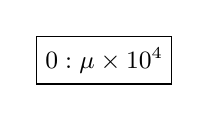
\begin{tikzpicture}
\small
\matrix[nodes={minimum size=6mm}] {
  \node[draw] {$0:\mu\times 10^4$};\\
};
\end{tikzpicture}

Note that the service rate is \textbf{multiplied by $10^4$} so that it can be
returned as an integer with 2 decimal points precision, for example if
$\mu=.1234$, then {\Tt{}\nwlinkedidentq{DBQueryMetricServiceRate}{NW1Dx1yV-48hNGo-1}\nwendquote}(1) returns $1234$.\\
\textbf{Side Effects:} none.\\
\textbf{Throws:} {\Tt{}SQLException\nwendquote} if database failure is encountered.\\
\bottomrule
\end{tabular}
\nwenddocs{}\nwbegincode{178}\sublabel{NW1Dx1yV-48hNGo-1}\nwmargintag{{\nwtagstyle{}\subpageref{NW1Dx1yV-48hNGo-1}}}\moddef{Read: DBQueryMetricServiceRate(1)~{\nwtagstyle{}\subpageref{NW1Dx1yV-48hNGo-1}}}\endmoddef\nwstartdeflinemarkup\nwusesondefline{\\{NW46kjAM-Oyob-1}}\nwenddeflinemarkup
int[] \nwlinkedidentc{DBQueryMetricServiceRate}{NW1Dx1yV-48hNGo-1}(boolean flag_usecache) throws SQLException \{
  int[] output = new int[] \{ \};
  if (flag_usecache) \{
    output = new int[] \{ (int) (10000*(this.count_assigned
        / (double) this.count_requests)) \};
  \} else \{
    try (\LA{}Open \code{}conn\edoc{}~{\nwtagstyle{}\subpageref{NW1ODIS0-JT1v9-1}}\RA{}) \{
      output = \nwlinkedidentc{PSQuery}{NW1ODIS0-yHOIP-1}(conn, "\nwlinkedidentc{S102}{NW1ODIS0-1RuRoZ-1}", 1);
    \} catch (SQLException e) \{
      throw e;
    \}
  \}
  return output;
\}
\nwindexdefn{\nwixident{DBQueryMetricServiceRate}}{DBQueryMetricServiceRate}{NW1Dx1yV-48hNGo-1}\eatline
\nwused{\\{NW46kjAM-Oyob-1}}\nwidentdefs{\\{{\nwixident{DBQueryMetricServiceRate}}{DBQueryMetricServiceRate}}}\nwidentuses{\\{{\nwixident{PSQuery}}{PSQuery}}\\{{\nwixident{S102}}{S102}}}\nwindexuse{\nwixident{PSQuery}}{PSQuery}{NW1Dx1yV-48hNGo-1}\nwindexuse{\nwixident{S102}}{S102}{NW1Dx1yV-48hNGo-1}\nwendcode{}\nwbegindocs{179}\begin{tabular}{p{\textwidth}}
\toprule
\rowcolor{TableTitle}
Method \textcolor{blue}{{\Tt{}\nwlinkedidentq{DBQueryMetricServiceRate}{NW1Dx1yV-48hNGo-1}\nwendquote}}(0) calls {\Tt{}\nwlinkedidentq{DBQueryMetricServiceRate}{NW1Dx1yV-48hNGo-1}\nwendquote}(1)
with a default parameter.\\
\bottomrule
\end{tabular}
\nwenddocs{}\nwbegincode{180}\sublabel{NW1Dx1yV-49bCCM-1}\nwmargintag{{\nwtagstyle{}\subpageref{NW1Dx1yV-49bCCM-1}}}\moddef{Read: DBQueryMetricServiceRate(0)~{\nwtagstyle{}\subpageref{NW1Dx1yV-49bCCM-1}}}\endmoddef\nwstartdeflinemarkup\nwusesondefline{\\{NW46kjAM-Oyob-2}}\nwenddeflinemarkup
int[] \nwlinkedidentc{DBQueryMetricServiceRate}{NW1Dx1yV-48hNGo-1}() throws SQLException \{
  return \nwlinkedidentc{DBQueryMetricServiceRate}{NW1Dx1yV-48hNGo-1}(true);
\}
\nwused{\\{NW46kjAM-Oyob-2}}\nwidentuses{\\{{\nwixident{DBQueryMetricServiceRate}}{DBQueryMetricServiceRate}}}\nwindexuse{\nwixident{DBQueryMetricServiceRate}}{DBQueryMetricServiceRate}{NW1Dx1yV-49bCCM-1}\nwendcode{}\nwbegindocs{181}\nwdocspar
\noindent
\begin{tabular}{p{\textwidth}}
\toprule
\rowcolor{TableTitle}
Method \textcolor{blue}{{\Tt{}\nwlinkedidentq{queryMetricServiceRate}{NW1Dx1yV-fqewh-1}\nwendquote}}(1) wraps {\Tt{}\nwlinkedidentq{DBQueryMetricServiceRate}{NW1Dx1yV-48hNGo-1}\nwendquote}(1).\\
\bottomrule
\end{tabular}
\nwenddocs{}\nwbegincode{182}\sublabel{NW1Dx1yV-fqewh-1}\nwmargintag{{\nwtagstyle{}\subpageref{NW1Dx1yV-fqewh-1}}}\moddef{Read: queryMetricServiceRate(1)~{\nwtagstyle{}\subpageref{NW1Dx1yV-fqewh-1}}}\endmoddef\nwstartdeflinemarkup\nwusesondefline{\\{NW3hMOhb-2u8vSA-1}}\nwenddeflinemarkup
int[] \nwlinkedidentc{queryMetricServiceRate}{NW1Dx1yV-fqewh-1}(boolean flag_usecache) throws SQLException \{
  int[] output = storage.\nwlinkedidentc{DBQueryMetricServiceRate}{NW1Dx1yV-48hNGo-1}(flag_usecache);
  return output;
\}
\nwindexdefn{\nwixident{queryMetricServiceRate}}{queryMetricServiceRate}{NW1Dx1yV-fqewh-1}\eatline
\nwused{\\{NW3hMOhb-2u8vSA-1}}\nwidentdefs{\\{{\nwixident{queryMetricServiceRate}}{queryMetricServiceRate}}}\nwidentuses{\\{{\nwixident{DBQueryMetricServiceRate}}{DBQueryMetricServiceRate}}}\nwindexuse{\nwixident{DBQueryMetricServiceRate}}{DBQueryMetricServiceRate}{NW1Dx1yV-fqewh-1}\nwendcode{}\nwbegindocs{183}\begin{tabular}{p{\textwidth}}
\toprule
\rowcolor{TableTitle}
Method \textcolor{blue}{{\Tt{}\nwlinkedidentq{queryMetricServiceRate}{NW1Dx1yV-fqewh-1}\nwendquote}}(0) calls {\Tt{}\nwlinkedidentq{queryMetricServiceRate}{NW1Dx1yV-fqewh-1}\nwendquote}(1)
with a default parameter.\\
\bottomrule
\end{tabular}
\nwenddocs{}\nwbegincode{184}\sublabel{NW1Dx1yV-f55U7-1}\nwmargintag{{\nwtagstyle{}\subpageref{NW1Dx1yV-f55U7-1}}}\moddef{Read: queryMetricServiceRate(0)~{\nwtagstyle{}\subpageref{NW1Dx1yV-f55U7-1}}}\endmoddef\nwstartdeflinemarkup\nwusesondefline{\\{NW3hMOhb-2u8vSA-2}}\nwenddeflinemarkup
int[] \nwlinkedidentc{queryMetricServiceRate}{NW1Dx1yV-fqewh-1}() throws SQLException \{
  return \nwlinkedidentc{queryMetricServiceRate}{NW1Dx1yV-fqewh-1}(true);
\}
\nwused{\\{NW3hMOhb-2u8vSA-2}}\nwidentuses{\\{{\nwixident{queryMetricServiceRate}}{queryMetricServiceRate}}}\nwindexuse{\nwixident{queryMetricServiceRate}}{queryMetricServiceRate}{NW1Dx1yV-f55U7-1}\nwendcode{}\nwbegindocs{185}\nwdocspar

\subsubsection{\texttt{DBQueryMetricServiceRateRunning}(0)}
\nwenddocs{}\nwbegincode{186}\sublabel{NW1Dx1yV-11FNsC-1}\nwmargintag{{\nwtagstyle{}\subpageref{NW1Dx1yV-11FNsC-1}}}\moddef{Read: DBQueryMetricServiceRateRunning(0)~{\nwtagstyle{}\subpageref{NW1Dx1yV-11FNsC-1}}}\endmoddef\nwstartdeflinemarkup\nwenddeflinemarkup
int[] \nwlinkedidentc{DBQueryMetricServiceRateRunning}{NW1Dx1yV-11FNsC-1}() throws SQLException \{
  int[] output = new int[] \{ \};
  // ...
  return output;
\}
\nwindexdefn{\nwixident{DBQueryMetricServiceRateRunning}}{DBQueryMetricServiceRateRunning}{NW1Dx1yV-11FNsC-1}\eatline
\nwnotused{Read: DBQueryMetricServiceRateRunning(0)}\nwidentdefs{\\{{\nwixident{DBQueryMetricServiceRateRunning}}{DBQueryMetricServiceRateRunning}}}\nwendcode{}\nwbegincode{187}\sublabel{NW1Dx1yV-3uM1ts-1}\nwmargintag{{\nwtagstyle{}\subpageref{NW1Dx1yV-3uM1ts-1}}}\moddef{Read: queryMetricServiceRateRunning(0)~{\nwtagstyle{}\subpageref{NW1Dx1yV-3uM1ts-1}}}\endmoddef\nwstartdeflinemarkup\nwusesondefline{\\{NW3hMOhb-2u8vSA-1}}\nwenddeflinemarkup
int[] \nwlinkedidentc{queryMetricServiceRateRunning}{NW1Dx1yV-3uM1ts-1}() throws SQLException \{
  int[] output = new int[] \{
      Math.min((int) (10000*(this.storage.\nwlinkedidentc{DBQueryRequestsCountAssigned}{NW1Dx1yV-2r5hKL-1}()[0]
        / (double) this.lu_rseen.size())), 10000) \};
  return output;
\}
\nwindexdefn{\nwixident{queryMetricServiceRateRunning}}{queryMetricServiceRateRunning}{NW1Dx1yV-3uM1ts-1}\eatline
\nwused{\\{NW3hMOhb-2u8vSA-1}}\nwidentdefs{\\{{\nwixident{queryMetricServiceRateRunning}}{queryMetricServiceRateRunning}}}\nwidentuses{\\{{\nwixident{DBQueryRequestsCountAssigned}}{DBQueryRequestsCountAssigned}}}\nwindexuse{\nwixident{DBQueryRequestsCountAssigned}}{DBQueryRequestsCountAssigned}{NW1Dx1yV-3uM1ts-1}\nwendcode{}\nwbegindocs{188}\nwdocspar
\subsubsection{\texttt{DBQueryMetricUserDistanceBaseTotal}(1)}
\begin{tabular}{p{\textwidth}}
\toprule
\rowcolor{TableTitle}
Method \textcolor{blue}{{\Tt{}\nwlinkedidentq{DBQueryMetricUserDistanceBaseTotal}{NW1Dx1yV-1YwEBe-1}\nwendquote}}(1) returns the
base distance $D^\textrm{base}(\mathcal{U})$ (Eq.~\ref{eq:base-distance}).
A {\Tt{}SQLException\nwendquote} is thrown in case of database failure.\\
\midrule
\textbf{Parameters:} none.\\
\textbf{Returns:} results of the query flattened into an integer array,
or {\Tt{}null\nwendquote} if no results.

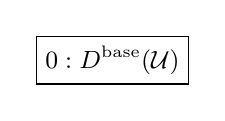
\begin{tikzpicture}
\small
\matrix[nodes={minimum size=6mm}] {
  \node[draw] {$0:D^\textrm{base}(\mathcal{U})$};\\
};
\end{tikzpicture}\\
\textbf{Side Effects:} none.\\
\textbf{Throws:} {\Tt{}SQLException\nwendquote} if database failure is encountered.\\
\bottomrule
\end{tabular}
\nwenddocs{}\nwbegincode{189}\sublabel{NW1Dx1yV-1YwEBe-1}\nwmargintag{{\nwtagstyle{}\subpageref{NW1Dx1yV-1YwEBe-1}}}\moddef{Read: DBQueryMetricUserDistanceBaseTotal(1)~{\nwtagstyle{}\subpageref{NW1Dx1yV-1YwEBe-1}}}\endmoddef\nwstartdeflinemarkup\nwusesondefline{\\{NW46kjAM-Oyob-1}}\nwenddeflinemarkup
int[] \nwlinkedidentc{DBQueryMetricUserDistanceBaseTotal}{NW1Dx1yV-1YwEBe-1}(boolean flag_usecache) throws SQLException \{
  if (flag_usecache) \{
    return new int[] \{ this.sum_distance_base_requests + this.sum_distance_base_servers \};
  \} else \{
    try (\LA{}Open \code{}conn\edoc{}~{\nwtagstyle{}\subpageref{NW1ODIS0-JT1v9-1}}\RA{}) \{
      return \nwlinkedidentc{PSQuery}{NW1ODIS0-yHOIP-1}(conn, "\nwlinkedidentc{S103}{NW1ODIS0-3POlUB-1}", 1);
    \} catch (SQLException e) \{
      throw e;
    \}
  \}
\}
\nwindexdefn{\nwixident{DBQueryMetricUserDistanceBaseTotal}}{DBQueryMetricUserDistanceBaseTotal}{NW1Dx1yV-1YwEBe-1}\eatline
\nwused{\\{NW46kjAM-Oyob-1}}\nwidentdefs{\\{{\nwixident{DBQueryMetricUserDistanceBaseTotal}}{DBQueryMetricUserDistanceBaseTotal}}}\nwidentuses{\\{{\nwixident{PSQuery}}{PSQuery}}\\{{\nwixident{S103}}{S103}}}\nwindexuse{\nwixident{PSQuery}}{PSQuery}{NW1Dx1yV-1YwEBe-1}\nwindexuse{\nwixident{S103}}{S103}{NW1Dx1yV-1YwEBe-1}\nwendcode{}\nwbegindocs{190}\begin{tabular}{p{\textwidth}}
\toprule
\rowcolor{TableTitle}
Method \textcolor{blue}{{\Tt{}\nwlinkedidentq{DBQueryMetricUserDistanceBaseTotal}{NW1Dx1yV-1YwEBe-1}\nwendquote}}(0) calls {\Tt{}\nwlinkedidentq{DBQueryMetricUserDistanceBaseTotal}{NW1Dx1yV-1YwEBe-1}\nwendquote}(1)
with a default parameter.\\
\bottomrule
\end{tabular}
\nwenddocs{}\nwbegincode{191}\sublabel{NW1Dx1yV-1ZAnmM-1}\nwmargintag{{\nwtagstyle{}\subpageref{NW1Dx1yV-1ZAnmM-1}}}\moddef{Read: DBQueryMetricUserDistanceBaseTotal(0)~{\nwtagstyle{}\subpageref{NW1Dx1yV-1ZAnmM-1}}}\endmoddef\nwstartdeflinemarkup\nwusesondefline{\\{NW46kjAM-Oyob-2}}\nwenddeflinemarkup
int[] \nwlinkedidentc{DBQueryMetricUserDistanceBaseTotal}{NW1Dx1yV-1YwEBe-1}() throws SQLException \{
  return \nwlinkedidentc{DBQueryMetricUserDistanceBaseTotal}{NW1Dx1yV-1YwEBe-1}(true);
\}
\nwused{\\{NW46kjAM-Oyob-2}}\nwidentuses{\\{{\nwixident{DBQueryMetricUserDistanceBaseTotal}}{DBQueryMetricUserDistanceBaseTotal}}}\nwindexuse{\nwixident{DBQueryMetricUserDistanceBaseTotal}}{DBQueryMetricUserDistanceBaseTotal}{NW1Dx1yV-1ZAnmM-1}\nwendcode{}\nwbegindocs{192}\nwdocspar
\noindent
\begin{tabular}{p{\textwidth}}
\toprule
\rowcolor{TableTitle}
Method \textcolor{blue}{{\Tt{}\nwlinkedidentq{queryMetricUserDistanceBaseTotal}{NW1Dx1yV-4D0ey0-1}\nwendquote}}(1) wraps {\Tt{}\nwlinkedidentq{DBQueryMetricUserDistanceBaseTotal}{NW1Dx1yV-1YwEBe-1}\nwendquote}(1).\\
\bottomrule
\end{tabular}
\nwenddocs{}\nwbegincode{193}\sublabel{NW1Dx1yV-4D0ey0-1}\nwmargintag{{\nwtagstyle{}\subpageref{NW1Dx1yV-4D0ey0-1}}}\moddef{Read: queryMetricUserDistanceBaseTotal(1)~{\nwtagstyle{}\subpageref{NW1Dx1yV-4D0ey0-1}}}\endmoddef\nwstartdeflinemarkup\nwusesondefline{\\{NW3hMOhb-2u8vSA-1}}\nwenddeflinemarkup
int[] \nwlinkedidentc{queryMetricUserDistanceBaseTotal}{NW1Dx1yV-4D0ey0-1}(boolean flag_usecache) throws SQLException \{
  int[] output = storage.\nwlinkedidentc{DBQueryMetricUserDistanceBaseTotal}{NW1Dx1yV-1YwEBe-1}(flag_usecache);
  return output;
\}
\nwindexdefn{\nwixident{queryMetricUserDistanceBaseTotal}}{queryMetricUserDistanceBaseTotal}{NW1Dx1yV-4D0ey0-1}\eatline
\nwused{\\{NW3hMOhb-2u8vSA-1}}\nwidentdefs{\\{{\nwixident{queryMetricUserDistanceBaseTotal}}{queryMetricUserDistanceBaseTotal}}}\nwidentuses{\\{{\nwixident{DBQueryMetricUserDistanceBaseTotal}}{DBQueryMetricUserDistanceBaseTotal}}}\nwindexuse{\nwixident{DBQueryMetricUserDistanceBaseTotal}}{DBQueryMetricUserDistanceBaseTotal}{NW1Dx1yV-4D0ey0-1}\nwendcode{}\nwbegindocs{194}\begin{tabular}{p{\textwidth}}
\toprule
\rowcolor{TableTitle}
Method \textcolor{blue}{{\Tt{}\nwlinkedidentq{queryMetricUserDistanceBaseTotal}{NW1Dx1yV-4D0ey0-1}\nwendquote}}(0) calls {\Tt{}\nwlinkedidentq{queryMetricUserDistanceBaseTotal}{NW1Dx1yV-4D0ey0-1}\nwendquote}(1)
with a default parameter.\\
\bottomrule
\end{tabular}
\nwenddocs{}\nwbegincode{195}\sublabel{NW1Dx1yV-4C6HwO-1}\nwmargintag{{\nwtagstyle{}\subpageref{NW1Dx1yV-4C6HwO-1}}}\moddef{Read: queryMetricUserDistanceBaseTotal(0)~{\nwtagstyle{}\subpageref{NW1Dx1yV-4C6HwO-1}}}\endmoddef\nwstartdeflinemarkup\nwusesondefline{\\{NW3hMOhb-2u8vSA-2}}\nwenddeflinemarkup
int[] \nwlinkedidentc{queryMetricUserDistanceBaseTotal}{NW1Dx1yV-4D0ey0-1}() throws SQLException \{
  return \nwlinkedidentc{queryMetricUserDistanceBaseTotal}{NW1Dx1yV-4D0ey0-1}(true);
\}
\nwused{\\{NW3hMOhb-2u8vSA-2}}\nwidentuses{\\{{\nwixident{queryMetricUserDistanceBaseTotal}}{queryMetricUserDistanceBaseTotal}}}\nwindexuse{\nwixident{queryMetricUserDistanceBaseTotal}}{queryMetricUserDistanceBaseTotal}{NW1Dx1yV-4C6HwO-1}\nwendcode{}\nwbegindocs{196}\nwdocspar

\subsubsection{\texttt{DBQueryMetricUserDistanceBaseRunning}(0)}
\nwenddocs{}\nwbegincode{197}\sublabel{NW1Dx1yV-Wa7Hh-1}\nwmargintag{{\nwtagstyle{}\subpageref{NW1Dx1yV-Wa7Hh-1}}}\moddef{Read: DBQueryMetricUserDistanceBaseRunning(0)~{\nwtagstyle{}\subpageref{NW1Dx1yV-Wa7Hh-1}}}\endmoddef\nwstartdeflinemarkup\nwusesondefline{\\{NW46kjAM-Oyob-1}}\nwenddeflinemarkup
int[] \nwlinkedidentc{DBQueryMetricUserDistanceBaseRunning}{NW1Dx1yV-Wa7Hh-1}() throws SQLException \{
  int[] output = new int[] \{ \};
  // ...
  return output;
\}
\nwindexdefn{\nwixident{DBQueryMetricUserDistanceBaseRunning}}{DBQueryMetricUserDistanceBaseRunning}{NW1Dx1yV-Wa7Hh-1}\eatline
\nwused{\\{NW46kjAM-Oyob-1}}\nwidentdefs{\\{{\nwixident{DBQueryMetricUserDistanceBaseRunning}}{DBQueryMetricUserDistanceBaseRunning}}}\nwendcode{}\nwbegincode{198}\sublabel{NW1Dx1yV-2kPye-1}\nwmargintag{{\nwtagstyle{}\subpageref{NW1Dx1yV-2kPye-1}}}\moddef{Read: queryMetricUserDistanceBaseRunning(0)~{\nwtagstyle{}\subpageref{NW1Dx1yV-2kPye-1}}}\endmoddef\nwstartdeflinemarkup\nwusesondefline{\\{NW3hMOhb-2u8vSA-1}}\nwenddeflinemarkup
int[] \nwlinkedidentc{queryMetricUserDistanceBaseRunning}{NW1Dx1yV-2kPye-1}()
throws SQLException, \nwlinkedidentc{UserNotFoundException}{NW1ODIS0-15irq2-1} \{
  int[] output = new int[] \{ 0 \};
  for (int sid : this.lu_sseen.keySet()) \{
    output[0] += this.storage.\nwlinkedidentc{DBQueryUser}{NW1Dx1yV-8IJdE-1}(sid)[6];
  \}
  for (int rid : this.lu_rseen.keySet()) \{
    output[0] += this.storage.\nwlinkedidentc{DBQueryUser}{NW1Dx1yV-8IJdE-1}(rid)[6];
  \}
  return output;
\}
\nwindexdefn{\nwixident{queryMetricUserDistanceBaseRunning}}{queryMetricUserDistanceBaseRunning}{NW1Dx1yV-2kPye-1}\eatline
\nwused{\\{NW3hMOhb-2u8vSA-1}}\nwidentdefs{\\{{\nwixident{queryMetricUserDistanceBaseRunning}}{queryMetricUserDistanceBaseRunning}}}\nwidentuses{\\{{\nwixident{DBQueryUser}}{DBQueryUser}}\\{{\nwixident{UserNotFoundException}}{UserNotFoundException}}}\nwindexuse{\nwixident{DBQueryUser}}{DBQueryUser}{NW1Dx1yV-2kPye-1}\nwindexuse{\nwixident{UserNotFoundException}}{UserNotFoundException}{NW1Dx1yV-2kPye-1}\nwendcode{}\nwbegindocs{199}\nwdocspar
\subsubsection{\texttt{DBQueryMetricServerDistanceTotal}(1)}
\begin{tabular}{p{\textwidth}}
\toprule
\rowcolor{TableTitle}
Method \textcolor{blue}{{\Tt{}\nwlinkedidentq{DBQueryMetricServerDistanceTotal}{NW1Dx1yV-46RFWc-1}\nwendquote}}(1) returns the
total travel distance of all the servers.
A {\Tt{}SQLException\nwendquote} is thrown in case of database failure.\\
\midrule
\textbf{Parameters:} none.\\
\textbf{Returns:} results of the query flattened into an integer array,
or {\Tt{}null\nwendquote} if no results.

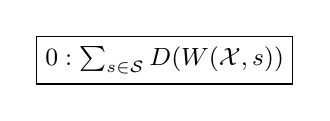
\begin{tikzpicture}
\small
\matrix[nodes={minimum size=6mm}] {
  \node[draw] {$0:\sum_{s\in\mathcal{S}}D(W(\mathcal{X},s))$};\\
};
\end{tikzpicture}\\
\textbf{Side Effects:} none.\\
\textbf{Throws:} {\Tt{}SQLException\nwendquote} if database failure is encountered.\\
\bottomrule
\end{tabular}
\nwenddocs{}\nwbegincode{200}\sublabel{NW1Dx1yV-46RFWc-1}\nwmargintag{{\nwtagstyle{}\subpageref{NW1Dx1yV-46RFWc-1}}}\moddef{Read: DBQueryMetricServerDistanceTotal(1)~{\nwtagstyle{}\subpageref{NW1Dx1yV-46RFWc-1}}}\endmoddef\nwstartdeflinemarkup\nwusesondefline{\\{NW46kjAM-Oyob-1}}\nwenddeflinemarkup
int[] \nwlinkedidentc{DBQueryMetricServerDistanceTotal}{NW1Dx1yV-46RFWc-1}(boolean flag_usecache) throws SQLException \{
  if (flag_usecache) \{
    final int[] output = new int[] \{ 0 \};
    this.distance_servers.forEach((sid, val) -> output[0] += val);
    return output;
  \} else \{
    try (\LA{}Open \code{}conn\edoc{}~{\nwtagstyle{}\subpageref{NW1ODIS0-JT1v9-1}}\RA{}) \{
      return \nwlinkedidentc{PSQuery}{NW1ODIS0-yHOIP-1}(conn, "\nwlinkedidentc{S105}{NW1ODIS0-4eK3jf-1}", 1);
    \} catch (SQLException e) \{
      throw e;
    \}
  \}
\}
\nwindexdefn{\nwixident{DBQueryMetricServerDistanceTotal}}{DBQueryMetricServerDistanceTotal}{NW1Dx1yV-46RFWc-1}\eatline
\nwused{\\{NW46kjAM-Oyob-1}}\nwidentdefs{\\{{\nwixident{DBQueryMetricServerDistanceTotal}}{DBQueryMetricServerDistanceTotal}}}\nwidentuses{\\{{\nwixident{PSQuery}}{PSQuery}}\\{{\nwixident{S105}}{S105}}}\nwindexuse{\nwixident{PSQuery}}{PSQuery}{NW1Dx1yV-46RFWc-1}\nwindexuse{\nwixident{S105}}{S105}{NW1Dx1yV-46RFWc-1}\nwendcode{}\nwbegindocs{201}\begin{tabular}{p{\textwidth}}
\toprule
\rowcolor{TableTitle}
Method \textcolor{blue}{{\Tt{}\nwlinkedidentq{DBQueryMetricServerDistanceTotal}{NW1Dx1yV-46RFWc-1}\nwendquote}}(0) calls {\Tt{}\nwlinkedidentq{DBQueryMetricServerDistanceTotal}{NW1Dx1yV-46RFWc-1}\nwendquote}(1)
with a default parameter.\\
\bottomrule
\end{tabular}
\nwenddocs{}\nwbegincode{202}\sublabel{NW1Dx1yV-47NowU-1}\nwmargintag{{\nwtagstyle{}\subpageref{NW1Dx1yV-47NowU-1}}}\moddef{Read: DBQueryMetricServerDistanceTotal(0)~{\nwtagstyle{}\subpageref{NW1Dx1yV-47NowU-1}}}\endmoddef\nwstartdeflinemarkup\nwusesondefline{\\{NW46kjAM-Oyob-2}}\nwenddeflinemarkup
int[] \nwlinkedidentc{DBQueryMetricServerDistanceTotal}{NW1Dx1yV-46RFWc-1}() throws SQLException \{
  return \nwlinkedidentc{DBQueryMetricServerDistanceTotal}{NW1Dx1yV-46RFWc-1}(true);
\}
\nwused{\\{NW46kjAM-Oyob-2}}\nwidentuses{\\{{\nwixident{DBQueryMetricServerDistanceTotal}}{DBQueryMetricServerDistanceTotal}}}\nwindexuse{\nwixident{DBQueryMetricServerDistanceTotal}}{DBQueryMetricServerDistanceTotal}{NW1Dx1yV-47NowU-1}\nwendcode{}\nwbegindocs{203}\nwdocspar
\noindent
\begin{tabular}{p{\textwidth}}
\toprule
\rowcolor{TableTitle}
Method \textcolor{blue}{{\Tt{}\nwlinkedidentq{queryMetricServerDistanceTotal}{NW1Dx1yV-4enTWS-1}\nwendquote}}(1) wraps {\Tt{}\nwlinkedidentq{DBQueryMetricServerDistanceTotal}{NW1Dx1yV-46RFWc-1}\nwendquote}(1).\\
\bottomrule
\end{tabular}
\nwenddocs{}\nwbegincode{204}\sublabel{NW1Dx1yV-4enTWS-1}\nwmargintag{{\nwtagstyle{}\subpageref{NW1Dx1yV-4enTWS-1}}}\moddef{Read: queryMetricServerDistanceTotal(1)~{\nwtagstyle{}\subpageref{NW1Dx1yV-4enTWS-1}}}\endmoddef\nwstartdeflinemarkup\nwusesondefline{\\{NW3hMOhb-2u8vSA-1}}\nwenddeflinemarkup
int[] \nwlinkedidentc{queryMetricServerDistanceTotal}{NW1Dx1yV-4enTWS-1}(boolean flag_usecache) throws SQLException \{
  int[] output = storage.\nwlinkedidentc{DBQueryMetricServerDistanceTotal}{NW1Dx1yV-46RFWc-1}(flag_usecache);
  return output;
\}
\nwindexdefn{\nwixident{queryMetricServerDistanceTotal}}{queryMetricServerDistanceTotal}{NW1Dx1yV-4enTWS-1}\eatline
\nwused{\\{NW3hMOhb-2u8vSA-1}}\nwidentdefs{\\{{\nwixident{queryMetricServerDistanceTotal}}{queryMetricServerDistanceTotal}}}\nwidentuses{\\{{\nwixident{DBQueryMetricServerDistanceTotal}}{DBQueryMetricServerDistanceTotal}}}\nwindexuse{\nwixident{DBQueryMetricServerDistanceTotal}}{DBQueryMetricServerDistanceTotal}{NW1Dx1yV-4enTWS-1}\nwendcode{}\nwbegindocs{205}\begin{tabular}{p{\textwidth}}
\toprule
\rowcolor{TableTitle}
Method \textcolor{blue}{{\Tt{}\nwlinkedidentq{queryMetricServerDistanceTotal}{NW1Dx1yV-4enTWS-1}\nwendquote}}(0) calls {\Tt{}\nwlinkedidentq{queryMetricServerDistanceTotal}{NW1Dx1yV-4enTWS-1}\nwendquote}(1)
with a default parameter.\\
\bottomrule
\end{tabular}
\nwenddocs{}\nwbegincode{206}\sublabel{NW1Dx1yV-4fAqgC-1}\nwmargintag{{\nwtagstyle{}\subpageref{NW1Dx1yV-4fAqgC-1}}}\moddef{Read: queryMetricServerDistanceTotal(0)~{\nwtagstyle{}\subpageref{NW1Dx1yV-4fAqgC-1}}}\endmoddef\nwstartdeflinemarkup\nwusesondefline{\\{NW3hMOhb-2u8vSA-2}}\nwenddeflinemarkup
int[] \nwlinkedidentc{queryMetricServerDistanceTotal}{NW1Dx1yV-4enTWS-1}() throws SQLException \{
  return \nwlinkedidentc{queryMetricServerDistanceTotal}{NW1Dx1yV-4enTWS-1}(true);
\}
\nwused{\\{NW3hMOhb-2u8vSA-2}}\nwidentuses{\\{{\nwixident{queryMetricServerDistanceTotal}}{queryMetricServerDistanceTotal}}}\nwindexuse{\nwixident{queryMetricServerDistanceTotal}}{queryMetricServerDistanceTotal}{NW1Dx1yV-4fAqgC-1}\nwendcode{}\nwbegindocs{207}\nwdocspar

\subsubsection{\texttt{DBQueryMetricServerDistanceRunning}(0)}
\nwenddocs{}\nwbegincode{208}\sublabel{NW1Dx1yV-1Ros9t-1}\nwmargintag{{\nwtagstyle{}\subpageref{NW1Dx1yV-1Ros9t-1}}}\moddef{Read: DBQueryMetricServerDistanceRunning(0)~{\nwtagstyle{}\subpageref{NW1Dx1yV-1Ros9t-1}}}\endmoddef\nwstartdeflinemarkup\nwusesondefline{\\{NW46kjAM-Oyob-1}}\nwenddeflinemarkup
int[] \nwlinkedidentc{DBQueryMetricServerDistanceRunning}{NW1Dx1yV-1Ros9t-1}() throws SQLException \{
  int[] output = new int[] \{ \};
  // ...
  return output;
\}
\nwindexdefn{\nwixident{DBQueryMetricServerDistanceRunning}}{DBQueryMetricServerDistanceRunning}{NW1Dx1yV-1Ros9t-1}\eatline
\nwused{\\{NW46kjAM-Oyob-1}}\nwidentdefs{\\{{\nwixident{DBQueryMetricServerDistanceRunning}}{DBQueryMetricServerDistanceRunning}}}\nwendcode{}\nwbegincode{209}\sublabel{NW1Dx1yV-4gDOQR-1}\nwmargintag{{\nwtagstyle{}\subpageref{NW1Dx1yV-4gDOQR-1}}}\moddef{Read: queryMetricServerDistanceRunning(0)~{\nwtagstyle{}\subpageref{NW1Dx1yV-4gDOQR-1}}}\endmoddef\nwstartdeflinemarkup\nwusesondefline{\\{NW3hMOhb-2u8vSA-1}}\nwenddeflinemarkup
int[] \nwlinkedidentc{queryMetricServerDistanceRunning}{NW1Dx1yV-4gDOQR-1}() throws SQLException \{
  int[] output = new int[] \{ 0 \};
  for (int sid : this.lu_sseen.keySet()) \{
    output[0] += this.storage.\nwlinkedidentc{DBQueryServerDistance}{NW1Dx1yV-bdI1v-1}(sid, true)[0];
  \}
  return output;
\}
\nwindexdefn{\nwixident{queryMetricServerDistanceRunning}}{queryMetricServerDistanceRunning}{NW1Dx1yV-4gDOQR-1}\eatline
\nwused{\\{NW3hMOhb-2u8vSA-1}}\nwidentdefs{\\{{\nwixident{queryMetricServerDistanceRunning}}{queryMetricServerDistanceRunning}}}\nwidentuses{\\{{\nwixident{DBQueryServerDistance}}{DBQueryServerDistance}}}\nwindexuse{\nwixident{DBQueryServerDistance}}{DBQueryServerDistance}{NW1Dx1yV-4gDOQR-1}\nwendcode{}\nwbegindocs{210}\nwdocspar
\subsubsection{\texttt{DBQueryMetricServerDistanceBaseTotal}(0)}
\begin{tabular}{p{\textwidth}}
\toprule
\rowcolor{TableTitle}
Method \textcolor{blue}{{\Tt{}\nwlinkedidentq{DBQueryMetricServerDistanceBaseTotal}{NW1Dx1yV-2gaNGt-1}\nwendquote}}(0) returns the
base distance of all the servers.
A {\Tt{}SQLException\nwendquote} is thrown in case of database failure.\\
\midrule
\textbf{Parameters:} none.\\
\textbf{Returns:} results of the query flattened into an integer array,
or {\Tt{}null\nwendquote} if no results.

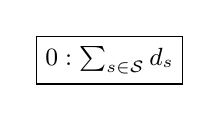
\begin{tikzpicture}
\small
\matrix[nodes={minimum size=6mm}] {
  \node[draw] {$0:\sum_{s\in\mathcal{S}}d_s$};\\
};
\end{tikzpicture}\\
\textbf{Side Effects:} none.\\
\textbf{Throws:} {\Tt{}SQLException\nwendquote} if database failure is encountered.\\
\bottomrule
\end{tabular}
\nwenddocs{}\nwbegincode{211}\sublabel{NW1Dx1yV-2gaNGt-1}\nwmargintag{{\nwtagstyle{}\subpageref{NW1Dx1yV-2gaNGt-1}}}\moddef{Read: DBQueryMetricServerDistanceBaseTotal(0)~{\nwtagstyle{}\subpageref{NW1Dx1yV-2gaNGt-1}}}\endmoddef\nwstartdeflinemarkup\nwusesondefline{\\{NW46kjAM-Oyob-1}}\nwenddeflinemarkup
int[] \nwlinkedidentc{DBQueryMetricServerDistanceBaseTotal}{NW1Dx1yV-2gaNGt-1}() throws SQLException \{
  // try (\LA{}Open \code{}conn\edoc{}~{\nwtagstyle{}\subpageref{NW1ODIS0-JT1v9-1}}\RA{}) \{
  //   return \nwlinkedidentc{PSQuery}{NW1ODIS0-yHOIP-1}(conn, "\nwlinkedidentc{S110}{NW1ODIS0-yTwJX-1}", 1);
  // \} catch (SQLException e) \{
  //   throw e;
  // \}
  return new int[] \{ this.sum_distance_base_servers \};
\}
\nwindexdefn{\nwixident{DBQueryMetricServerDistanceBaseTotal}}{DBQueryMetricServerDistanceBaseTotal}{NW1Dx1yV-2gaNGt-1}\eatline
\nwused{\\{NW46kjAM-Oyob-1}}\nwidentdefs{\\{{\nwixident{DBQueryMetricServerDistanceBaseTotal}}{DBQueryMetricServerDistanceBaseTotal}}}\nwidentuses{\\{{\nwixident{PSQuery}}{PSQuery}}\\{{\nwixident{S110}}{S110}}}\nwindexuse{\nwixident{PSQuery}}{PSQuery}{NW1Dx1yV-2gaNGt-1}\nwindexuse{\nwixident{S110}}{S110}{NW1Dx1yV-2gaNGt-1}\nwendcode{}\nwbegindocs{212}\begin{tabular}{p{\textwidth}}
\toprule
\rowcolor{TableTitle}
Method \textcolor{blue}{{\Tt{}\nwlinkedidentq{queryMetricServerDistanceBaseTotal}{NW1Dx1yV-2ZOFmc-1}\nwendquote}}(0) wraps {\Tt{}\nwlinkedidentq{DBQueryMetricServerDistanceBaseTotal}{NW1Dx1yV-2gaNGt-1}\nwendquote}(0).\\
\bottomrule
\end{tabular}
\nwenddocs{}\nwbegincode{213}\sublabel{NW1Dx1yV-2ZOFmc-1}\nwmargintag{{\nwtagstyle{}\subpageref{NW1Dx1yV-2ZOFmc-1}}}\moddef{Read: queryMetricServerDistanceBaseTotal(0)~{\nwtagstyle{}\subpageref{NW1Dx1yV-2ZOFmc-1}}}\endmoddef\nwstartdeflinemarkup\nwusesondefline{\\{NW3hMOhb-2u8vSA-1}}\nwenddeflinemarkup
int[] \nwlinkedidentc{queryMetricServerDistanceBaseTotal}{NW1Dx1yV-2ZOFmc-1}() throws SQLException \{
  int[] output = storage.\nwlinkedidentc{DBQueryMetricServerDistanceBaseTotal}{NW1Dx1yV-2gaNGt-1}();
  return output;
\}
\nwindexdefn{\nwixident{queryMetricServerDistanceBaseTotal}}{queryMetricServerDistanceBaseTotal}{NW1Dx1yV-2ZOFmc-1}\eatline
\nwused{\\{NW3hMOhb-2u8vSA-1}}\nwidentdefs{\\{{\nwixident{queryMetricServerDistanceBaseTotal}}{queryMetricServerDistanceBaseTotal}}}\nwidentuses{\\{{\nwixident{DBQueryMetricServerDistanceBaseTotal}}{DBQueryMetricServerDistanceBaseTotal}}}\nwindexuse{\nwixident{DBQueryMetricServerDistanceBaseTotal}}{DBQueryMetricServerDistanceBaseTotal}{NW1Dx1yV-2ZOFmc-1}\nwendcode{}\nwbegindocs{214}\nwdocspar
\subsubsection{\texttt{DBQueryMetricServerDistanceCruisingTotal}(1)}
\begin{tabular}{p{\textwidth}}
\toprule
\rowcolor{TableTitle}
Method \textcolor{blue}{{\Tt{}\nwlinkedidentq{DBQueryMetricServerDistanceCruisingTotal}{NW1Dx1yV-3ERM24-1}\nwendquote}}(1) returns the
total cruising distance of all servers.
A {\Tt{}SQLException\nwendquote} is thrown in case of database failure.\\
\midrule
\textbf{Parameters:} none.\\
\textbf{Returns:} results of the query flattened into an integer array,
or {\Tt{}null\nwendquote} if no results.

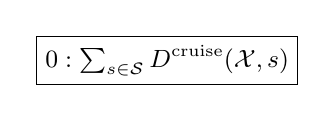
\begin{tikzpicture}
\small
\matrix[nodes={minimum size=6mm}] {
  \node[draw] {$0:\sum_{s\in\mathcal{S}}D^\textrm{cruise}(\mathcal{X},s)$};\\
};
\end{tikzpicture}\\
\textbf{Side Effects:} none.\\
\textbf{Throws:} {\Tt{}SQLException\nwendquote} if database failure is encountered.\\
\bottomrule
\end{tabular}
\nwenddocs{}\nwbegincode{215}\sublabel{NW1Dx1yV-3ERM24-1}\nwmargintag{{\nwtagstyle{}\subpageref{NW1Dx1yV-3ERM24-1}}}\moddef{Read: DBQueryMetricServerDistanceCruisingTotal(1)~{\nwtagstyle{}\subpageref{NW1Dx1yV-3ERM24-1}}}\endmoddef\nwstartdeflinemarkup\nwusesondefline{\\{NW46kjAM-Oyob-1}}\nwenddeflinemarkup
int[] \nwlinkedidentc{DBQueryMetricServerDistanceCruisingTotal}{NW1Dx1yV-3ERM24-1}(boolean flag_usecache) throws SQLException \{
  if (flag_usecache) \{
    final int[] output = new int[] \{ 0 \};
    this.distance_servers_cruising.forEach((sid, val) -> output[0] += val);
    return output;
  \} else \{
    try (\LA{}Open \code{}conn\edoc{}~{\nwtagstyle{}\subpageref{NW1ODIS0-JT1v9-1}}\RA{}) \{
      return \nwlinkedidentc{PSQuery}{NW1ODIS0-yHOIP-1}(conn, "\nwlinkedidentc{S107}{NW1ODIS0-2TmC55-1}", 1);
    \} catch (SQLException e) \{
      throw e;
    \}
  \}
\}
\nwindexdefn{\nwixident{DBQueryMetricServerDistanceCruisingTotal}}{DBQueryMetricServerDistanceCruisingTotal}{NW1Dx1yV-3ERM24-1}\eatline
\nwused{\\{NW46kjAM-Oyob-1}}\nwidentdefs{\\{{\nwixident{DBQueryMetricServerDistanceCruisingTotal}}{DBQueryMetricServerDistanceCruisingTotal}}}\nwidentuses{\\{{\nwixident{PSQuery}}{PSQuery}}\\{{\nwixident{S107}}{S107}}}\nwindexuse{\nwixident{PSQuery}}{PSQuery}{NW1Dx1yV-3ERM24-1}\nwindexuse{\nwixident{S107}}{S107}{NW1Dx1yV-3ERM24-1}\nwendcode{}\nwbegindocs{216}\begin{tabular}{p{\textwidth}}
\toprule
\rowcolor{TableTitle}
Method \textcolor{blue}{{\Tt{}\nwlinkedidentq{DBQueryMetricServerDistanceCruisingTotal}{NW1Dx1yV-3ERM24-1}\nwendquote}}(0) calls {\Tt{}\nwlinkedidentq{DBQueryMetricServerDistanceCruisingTotal}{NW1Dx1yV-3ERM24-1}\nwendquote}(1)
with a default parameter.\\
\bottomrule
\end{tabular}
\nwenddocs{}\nwbegincode{217}\sublabel{NW1Dx1yV-3ENmOe-1}\nwmargintag{{\nwtagstyle{}\subpageref{NW1Dx1yV-3ENmOe-1}}}\moddef{Read: DBQueryMetricServerDistanceCruisingTotal(0)~{\nwtagstyle{}\subpageref{NW1Dx1yV-3ENmOe-1}}}\endmoddef\nwstartdeflinemarkup\nwusesondefline{\\{NW46kjAM-Oyob-2}}\nwenddeflinemarkup
int[] \nwlinkedidentc{DBQueryMetricServerDistanceCruisingTotal}{NW1Dx1yV-3ERM24-1}() throws SQLException \{
  return \nwlinkedidentc{DBQueryMetricServerDistanceCruisingTotal}{NW1Dx1yV-3ERM24-1}(true);
\}
\nwused{\\{NW46kjAM-Oyob-2}}\nwidentuses{\\{{\nwixident{DBQueryMetricServerDistanceCruisingTotal}}{DBQueryMetricServerDistanceCruisingTotal}}}\nwindexuse{\nwixident{DBQueryMetricServerDistanceCruisingTotal}}{DBQueryMetricServerDistanceCruisingTotal}{NW1Dx1yV-3ENmOe-1}\nwendcode{}\nwbegindocs{218}\nwdocspar
\noindent
\begin{tabular}{p{\textwidth}}
\toprule
\rowcolor{TableTitle}
Method \textcolor{blue}{{\Tt{}\nwlinkedidentq{queryMetricServerDistanceCruisingTotal}{NW1Dx1yV-2UJeSo-1}\nwendquote}}(1) wraps {\Tt{}\nwlinkedidentq{DBQueryMetricServerDistanceCruisingTotal}{NW1Dx1yV-3ERM24-1}\nwendquote}(1).\\
\bottomrule
\end{tabular}
\nwenddocs{}\nwbegincode{219}\sublabel{NW1Dx1yV-2UJeSo-1}\nwmargintag{{\nwtagstyle{}\subpageref{NW1Dx1yV-2UJeSo-1}}}\moddef{Read: queryMetricServerDistanceCruisingTotal(1)~{\nwtagstyle{}\subpageref{NW1Dx1yV-2UJeSo-1}}}\endmoddef\nwstartdeflinemarkup\nwusesondefline{\\{NW3hMOhb-2u8vSA-1}}\nwenddeflinemarkup
int[] \nwlinkedidentc{queryMetricServerDistanceCruisingTotal}{NW1Dx1yV-2UJeSo-1}(boolean flag_usecache) throws SQLException \{
  int[] output = storage.\nwlinkedidentc{DBQueryMetricServerDistanceCruisingTotal}{NW1Dx1yV-3ERM24-1}(flag_usecache);
  return output;
\}
\nwindexdefn{\nwixident{queryMetricServerDistanceCruisingTotal}}{queryMetricServerDistanceCruisingTotal}{NW1Dx1yV-2UJeSo-1}\eatline
\nwused{\\{NW3hMOhb-2u8vSA-1}}\nwidentdefs{\\{{\nwixident{queryMetricServerDistanceCruisingTotal}}{queryMetricServerDistanceCruisingTotal}}}\nwidentuses{\\{{\nwixident{DBQueryMetricServerDistanceCruisingTotal}}{DBQueryMetricServerDistanceCruisingTotal}}}\nwindexuse{\nwixident{DBQueryMetricServerDistanceCruisingTotal}}{DBQueryMetricServerDistanceCruisingTotal}{NW1Dx1yV-2UJeSo-1}\nwendcode{}\nwbegindocs{220}\begin{tabular}{p{\textwidth}}
\toprule
\rowcolor{TableTitle}
Method \textcolor{blue}{{\Tt{}\nwlinkedidentq{queryMetricServerDistanceCruisingTotal}{NW1Dx1yV-2UJeSo-1}\nwendquote}}(0) calls {\Tt{}\nwlinkedidentq{queryMetricServerDistanceCruisingTotal}{NW1Dx1yV-2UJeSo-1}\nwendquote}(1)
with a default parameter.\\
\bottomrule
\end{tabular}
\nwenddocs{}\nwbegincode{221}\sublabel{NW1Dx1yV-2TPHRC-1}\nwmargintag{{\nwtagstyle{}\subpageref{NW1Dx1yV-2TPHRC-1}}}\moddef{Read: queryMetricServerDistanceCruisingTotal(0)~{\nwtagstyle{}\subpageref{NW1Dx1yV-2TPHRC-1}}}\endmoddef\nwstartdeflinemarkup\nwusesondefline{\\{NW3hMOhb-2u8vSA-2}}\nwenddeflinemarkup
int[] \nwlinkedidentc{queryMetricServerDistanceCruisingTotal}{NW1Dx1yV-2UJeSo-1}() throws SQLException \{
  return \nwlinkedidentc{queryMetricServerDistanceCruisingTotal}{NW1Dx1yV-2UJeSo-1}(true);
\}
\nwused{\\{NW3hMOhb-2u8vSA-2}}\nwidentuses{\\{{\nwixident{queryMetricServerDistanceCruisingTotal}}{queryMetricServerDistanceCruisingTotal}}}\nwindexuse{\nwixident{queryMetricServerDistanceCruisingTotal}}{queryMetricServerDistanceCruisingTotal}{NW1Dx1yV-2TPHRC-1}\nwendcode{}\nwbegindocs{222}\nwdocspar

\subsubsection{\texttt{DBQueryMetricServerDistanceServiceTotal}(1)}
\begin{tabular}{p{\textwidth}}
\toprule
\rowcolor{TableTitle}
Method \textcolor{blue}{{\Tt{}\nwlinkedidentq{DBQueryMetricServerDistanceServiceTotal}{NW1Dx1yV-42gXBD-1}\nwendquote}}(1) returns the
total service distance of all servers.
A {\Tt{}SQLException\nwendquote} is thrown in case of database failure.\\
\midrule
\textbf{Parameters:} none.\\
\textbf{Returns:} results of the query flattened into an integer array,
or {\Tt{}null\nwendquote} if no results.

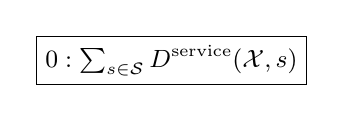
\begin{tikzpicture}
\small
\matrix[nodes={minimum size=6mm}] {
  \node[draw] {$0:\sum_{s\in\mathcal{S}}D^\textrm{service}(\mathcal{X},s)$};\\
};
\end{tikzpicture}\\
\textbf{Side Effects:} none.\\
\textbf{Throws:} {\Tt{}SQLException\nwendquote} if database failure is encountered.\\
\bottomrule
\end{tabular}
\nwenddocs{}\nwbegincode{223}\sublabel{NW1Dx1yV-42gXBD-1}\nwmargintag{{\nwtagstyle{}\subpageref{NW1Dx1yV-42gXBD-1}}}\moddef{Read: DBQueryMetricServerDistanceServiceTotal(1)~{\nwtagstyle{}\subpageref{NW1Dx1yV-42gXBD-1}}}\endmoddef\nwstartdeflinemarkup\nwusesondefline{\\{NW46kjAM-Oyob-1}}\nwenddeflinemarkup
int[] \nwlinkedidentc{DBQueryMetricServerDistanceServiceTotal}{NW1Dx1yV-42gXBD-1}(boolean flag_usecache) throws SQLException \{
  if (flag_usecache) \{
    final int[] output = new int[] \{ 0 \};
    this.distance_servers.forEach((sid, val) -> output[0] += (val - this.distance_servers_cruising.get(sid)));
    return output;
  \} else \{
    try (\LA{}Open \code{}conn\edoc{}~{\nwtagstyle{}\subpageref{NW1ODIS0-JT1v9-1}}\RA{}) \{
      return \nwlinkedidentc{PSQuery}{NW1ODIS0-yHOIP-1}(conn, "\nwlinkedidentc{S109}{NW1ODIS0-448CeR-1}", 1);
    \} catch (SQLException e) \{
      throw e;
    \}
  \}
\}
\nwindexdefn{\nwixident{DBQueryMetricServerDistanceServiceTotal}}{DBQueryMetricServerDistanceServiceTotal}{NW1Dx1yV-42gXBD-1}\eatline
\nwused{\\{NW46kjAM-Oyob-1}}\nwidentdefs{\\{{\nwixident{DBQueryMetricServerDistanceServiceTotal}}{DBQueryMetricServerDistanceServiceTotal}}}\nwidentuses{\\{{\nwixident{PSQuery}}{PSQuery}}\\{{\nwixident{S109}}{S109}}}\nwindexuse{\nwixident{PSQuery}}{PSQuery}{NW1Dx1yV-42gXBD-1}\nwindexuse{\nwixident{S109}}{S109}{NW1Dx1yV-42gXBD-1}\nwendcode{}\nwbegindocs{224}\begin{tabular}{p{\textwidth}}
\toprule
\rowcolor{TableTitle}
Method \textcolor{blue}{{\Tt{}\nwlinkedidentq{DBQueryMetricServerDistanceServiceTotal}{NW1Dx1yV-42gXBD-1}\nwendquote}}(0) calls {\Tt{}\nwlinkedidentq{DBQueryMetricServerDistanceServiceTotal}{NW1Dx1yV-42gXBD-1}\nwendquote}(1)
with a default parameter.\\
\bottomrule
\end{tabular}
\nwenddocs{}\nwbegincode{225}\sublabel{NW1Dx1yV-423lHf-1}\nwmargintag{{\nwtagstyle{}\subpageref{NW1Dx1yV-423lHf-1}}}\moddef{Read: DBQueryMetricServerDistanceServiceTotal(0)~{\nwtagstyle{}\subpageref{NW1Dx1yV-423lHf-1}}}\endmoddef\nwstartdeflinemarkup\nwusesondefline{\\{NW46kjAM-Oyob-2}}\nwenddeflinemarkup
int[] \nwlinkedidentc{DBQueryMetricServerDistanceServiceTotal}{NW1Dx1yV-42gXBD-1}() throws SQLException \{
  return \nwlinkedidentc{DBQueryMetricServerDistanceServiceTotal}{NW1Dx1yV-42gXBD-1}(true);
\}
\nwused{\\{NW46kjAM-Oyob-2}}\nwidentuses{\\{{\nwixident{DBQueryMetricServerDistanceServiceTotal}}{DBQueryMetricServerDistanceServiceTotal}}}\nwindexuse{\nwixident{DBQueryMetricServerDistanceServiceTotal}}{DBQueryMetricServerDistanceServiceTotal}{NW1Dx1yV-423lHf-1}\nwendcode{}\nwbegindocs{226}\nwdocspar
\noindent
\begin{tabular}{p{\textwidth}}
\toprule
\rowcolor{TableTitle}
Method \textcolor{blue}{{\Tt{}\nwlinkedidentq{queryMetricServerDistanceServiceTotal}{NW1Dx1yV-148TsN-1}\nwendquote}}(1) wraps {\Tt{}\nwlinkedidentq{DBQueryMetricServerDistanceServiceTotal}{NW1Dx1yV-42gXBD-1}\nwendquote}(1).\\
\bottomrule
\end{tabular}
\nwenddocs{}\nwbegincode{227}\sublabel{NW1Dx1yV-148TsN-1}\nwmargintag{{\nwtagstyle{}\subpageref{NW1Dx1yV-148TsN-1}}}\moddef{Read: queryMetricServerDistanceServiceTotal(1)~{\nwtagstyle{}\subpageref{NW1Dx1yV-148TsN-1}}}\endmoddef\nwstartdeflinemarkup\nwusesondefline{\\{NW3hMOhb-2u8vSA-1}}\nwenddeflinemarkup
int[] \nwlinkedidentc{queryMetricServerDistanceServiceTotal}{NW1Dx1yV-148TsN-1}(boolean flag_usecache) throws SQLException \{
  int[] output = storage.\nwlinkedidentc{DBQueryMetricServerDistanceServiceTotal}{NW1Dx1yV-42gXBD-1}(flag_usecache);
  return output;
\}
\nwindexdefn{\nwixident{queryMetricServerDistanceServiceTotal}}{queryMetricServerDistanceServiceTotal}{NW1Dx1yV-148TsN-1}\eatline
\nwused{\\{NW3hMOhb-2u8vSA-1}}\nwidentdefs{\\{{\nwixident{queryMetricServerDistanceServiceTotal}}{queryMetricServerDistanceServiceTotal}}}\nwidentuses{\\{{\nwixident{DBQueryMetricServerDistanceServiceTotal}}{DBQueryMetricServerDistanceServiceTotal}}}\nwindexuse{\nwixident{DBQueryMetricServerDistanceServiceTotal}}{DBQueryMetricServerDistanceServiceTotal}{NW1Dx1yV-148TsN-1}\nwendcode{}\nwbegindocs{228}\begin{tabular}{p{\textwidth}}
\toprule
\rowcolor{TableTitle}
Method \textcolor{blue}{{\Tt{}\nwlinkedidentq{queryMetricServerDistanceServiceTotal}{NW1Dx1yV-148TsN-1}\nwendquote}}(0) calls {\Tt{}\nwlinkedidentq{queryMetricServerDistanceServiceTotal}{NW1Dx1yV-148TsN-1}\nwendquote}(1)
with a default parameter.\\
\bottomrule
\end{tabular}
\nwenddocs{}\nwbegincode{229}\sublabel{NW1Dx1yV-14khfr-1}\nwmargintag{{\nwtagstyle{}\subpageref{NW1Dx1yV-14khfr-1}}}\moddef{Read: queryMetricServerDistanceServiceTotal(0)~{\nwtagstyle{}\subpageref{NW1Dx1yV-14khfr-1}}}\endmoddef\nwstartdeflinemarkup\nwusesondefline{\\{NW3hMOhb-2u8vSA-2}}\nwenddeflinemarkup
int[] \nwlinkedidentc{queryMetricServerDistanceServiceTotal}{NW1Dx1yV-148TsN-1}() throws SQLException \{
  return \nwlinkedidentc{queryMetricServerDistanceServiceTotal}{NW1Dx1yV-148TsN-1}(true);
\}
\nwused{\\{NW3hMOhb-2u8vSA-2}}\nwidentuses{\\{{\nwixident{queryMetricServerDistanceServiceTotal}}{queryMetricServerDistanceServiceTotal}}}\nwindexuse{\nwixident{queryMetricServerDistanceServiceTotal}}{queryMetricServerDistanceServiceTotal}{NW1Dx1yV-14khfr-1}\nwendcode{}\nwbegindocs{230}\nwdocspar

\subsubsection{\texttt{DBQueryMetricServerDurationTravelTotal}(1)}
\begin{tabular}{p{\textwidth}}
\toprule
\rowcolor{TableTitle}
Method \textcolor{blue}{{\Tt{}\nwlinkedidentq{DBQueryMetricServerDurationTravelTotal}{NW1Dx1yV-4T5Zjo-1}\nwendquote}}(1) returns the
total travel duration of all servers.
A {\Tt{}SQLException\nwendquote} is thrown in case of database failure.\\
\midrule
\textbf{Parameters:} none.\\
\textbf{Returns:} results of the query flattened into an integer array,
or {\Tt{}null\nwendquote} if no results.

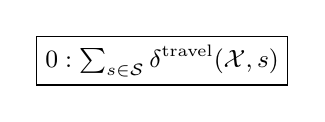
\begin{tikzpicture}
\small
\matrix[nodes={minimum size=6mm}] {
  \node[draw] {$0:\sum_{s\in\mathcal{S}}\delta^\textrm{travel}(\mathcal{X},s)$};\\
};
\end{tikzpicture}\\
\textbf{Side Effects:} none.\\
\textbf{Throws:} {\Tt{}SQLException\nwendquote} if database failure is encountered.\\
\bottomrule
\end{tabular}
\nwenddocs{}\nwbegincode{231}\sublabel{NW1Dx1yV-4T5Zjo-1}\nwmargintag{{\nwtagstyle{}\subpageref{NW1Dx1yV-4T5Zjo-1}}}\moddef{Read: DBQueryMetricServerDurationTravelTotal(1)~{\nwtagstyle{}\subpageref{NW1Dx1yV-4T5Zjo-1}}}\endmoddef\nwstartdeflinemarkup\nwusesondefline{\\{NW46kjAM-Oyob-1}}\nwenddeflinemarkup
int[] \nwlinkedidentc{DBQueryMetricServerDurationTravelTotal}{NW1Dx1yV-4T5Zjo-1}(boolean flag_usecache) throws SQLException \{
  if (flag_usecache) \{
    final int[] output = new int[] \{ 0 \};
    this.duration_servers.forEach((sid, val) -> output[0] += val);
    return output;
  \} else \{
    try (\LA{}Open \code{}conn\edoc{}~{\nwtagstyle{}\subpageref{NW1ODIS0-JT1v9-1}}\RA{}) \{
      return \nwlinkedidentc{PSQuery}{NW1ODIS0-yHOIP-1}(conn, "\nwlinkedidentc{S117}{NW1ODIS0-2Try6l-1}", 1);
    \} catch (SQLException e) \{
      throw e;
    \}
  \}
\}
\nwindexdefn{\nwixident{DBQueryMetricServerDurationTravelTotal}}{DBQueryMetricServerDurationTravelTotal}{NW1Dx1yV-4T5Zjo-1}\eatline
\nwused{\\{NW46kjAM-Oyob-1}}\nwidentdefs{\\{{\nwixident{DBQueryMetricServerDurationTravelTotal}}{DBQueryMetricServerDurationTravelTotal}}}\nwidentuses{\\{{\nwixident{PSQuery}}{PSQuery}}\\{{\nwixident{S117}}{S117}}}\nwindexuse{\nwixident{PSQuery}}{PSQuery}{NW1Dx1yV-4T5Zjo-1}\nwindexuse{\nwixident{S117}}{S117}{NW1Dx1yV-4T5Zjo-1}\nwendcode{}\nwbegindocs{232}\begin{tabular}{p{\textwidth}}
\toprule
\rowcolor{TableTitle}
Method \textcolor{blue}{{\Tt{}\nwlinkedidentq{DBQueryMetricServerDurationTravelTotal}{NW1Dx1yV-4T5Zjo-1}\nwendquote}}(0) calls {\Tt{}\nwlinkedidentq{DBQueryMetricServerDurationTravelTotal}{NW1Dx1yV-4T5Zjo-1}\nwendquote}(1)
with a default parameter.\\
\bottomrule
\end{tabular}
\nwenddocs{}\nwbegincode{233}\sublabel{NW1Dx1yV-4UAOce-1}\nwmargintag{{\nwtagstyle{}\subpageref{NW1Dx1yV-4UAOce-1}}}\moddef{Read: DBQueryMetricServerDurationTravelTotal(0)~{\nwtagstyle{}\subpageref{NW1Dx1yV-4UAOce-1}}}\endmoddef\nwstartdeflinemarkup\nwusesondefline{\\{NW46kjAM-Oyob-2}}\nwenddeflinemarkup
int[] \nwlinkedidentc{DBQueryMetricServerDurationTravelTotal}{NW1Dx1yV-4T5Zjo-1}() throws SQLException \{
  return \nwlinkedidentc{DBQueryMetricServerDurationTravelTotal}{NW1Dx1yV-4T5Zjo-1}(true);
\}
\nwused{\\{NW46kjAM-Oyob-2}}\nwidentuses{\\{{\nwixident{DBQueryMetricServerDurationTravelTotal}}{DBQueryMetricServerDurationTravelTotal}}}\nwindexuse{\nwixident{DBQueryMetricServerDurationTravelTotal}}{DBQueryMetricServerDurationTravelTotal}{NW1Dx1yV-4UAOce-1}\nwendcode{}\nwbegindocs{234}\nwdocspar
\noindent
\begin{tabular}{p{\textwidth}}
\toprule
\rowcolor{TableTitle}
Method \textcolor{blue}{{\Tt{}\nwlinkedidentq{queryMetricServerDurationTravelTotal}{NW1Dx1yV-3joACb-1}\nwendquote}}(1) wraps {\Tt{}\nwlinkedidentq{DBQueryMetricServerDurationTravelTotal}{NW1Dx1yV-4T5Zjo-1}\nwendquote}(1).\\
\bottomrule
\end{tabular}
\nwenddocs{}\nwbegincode{235}\sublabel{NW1Dx1yV-3joACb-1}\nwmargintag{{\nwtagstyle{}\subpageref{NW1Dx1yV-3joACb-1}}}\moddef{Read: queryMetricServerDurationTravelTotal(1)~{\nwtagstyle{}\subpageref{NW1Dx1yV-3joACb-1}}}\endmoddef\nwstartdeflinemarkup\nwusesondefline{\\{NW3hMOhb-2u8vSA-1}}\nwenddeflinemarkup
int[] \nwlinkedidentc{queryMetricServerDurationTravelTotal}{NW1Dx1yV-3joACb-1}(boolean flag_usecache) throws SQLException \{
  int[] output = storage.\nwlinkedidentc{DBQueryMetricServerDurationTravelTotal}{NW1Dx1yV-4T5Zjo-1}(flag_usecache);
  return output;
\}
\nwindexdefn{\nwixident{queryMetricServerDurationTravelTotal}}{queryMetricServerDurationTravelTotal}{NW1Dx1yV-3joACb-1}\eatline
\nwused{\\{NW3hMOhb-2u8vSA-1}}\nwidentdefs{\\{{\nwixident{queryMetricServerDurationTravelTotal}}{queryMetricServerDurationTravelTotal}}}\nwidentuses{\\{{\nwixident{DBQueryMetricServerDurationTravelTotal}}{DBQueryMetricServerDurationTravelTotal}}}\nwindexuse{\nwixident{DBQueryMetricServerDurationTravelTotal}}{DBQueryMetricServerDurationTravelTotal}{NW1Dx1yV-3joACb-1}\nwendcode{}\nwbegindocs{236}\begin{tabular}{p{\textwidth}}
\toprule
\rowcolor{TableTitle}
Method \textcolor{blue}{{\Tt{}\nwlinkedidentq{queryMetricServerDurationTravelTotal}{NW1Dx1yV-3joACb-1}\nwendquote}}(0) calls {\Tt{}\nwlinkedidentq{queryMetricServerDurationTravelTotal}{NW1Dx1yV-3joACb-1}\nwendquote}(1)
with a default parameter.\\
\bottomrule
\end{tabular}
\nwenddocs{}\nwbegincode{237}\sublabel{NW1Dx1yV-3kbNxN-1}\nwmargintag{{\nwtagstyle{}\subpageref{NW1Dx1yV-3kbNxN-1}}}\moddef{Read: queryMetricServerDurationTravelTotal(0)~{\nwtagstyle{}\subpageref{NW1Dx1yV-3kbNxN-1}}}\endmoddef\nwstartdeflinemarkup\nwusesondefline{\\{NW3hMOhb-2u8vSA-2}}\nwenddeflinemarkup
int[] \nwlinkedidentc{queryMetricServerDurationTravelTotal}{NW1Dx1yV-3joACb-1}() throws SQLException \{
  return \nwlinkedidentc{queryMetricServerDurationTravelTotal}{NW1Dx1yV-3joACb-1}(true);
\}
\nwused{\\{NW3hMOhb-2u8vSA-2}}\nwidentuses{\\{{\nwixident{queryMetricServerDurationTravelTotal}}{queryMetricServerDurationTravelTotal}}}\nwindexuse{\nwixident{queryMetricServerDurationTravelTotal}}{queryMetricServerDurationTravelTotal}{NW1Dx1yV-3kbNxN-1}\nwendcode{}\nwbegindocs{238}\nwdocspar

\subsubsection{\texttt{DBQueryMetricServerDurationCruisingTotal}(1)}
\nwenddocs{}\nwbegincode{239}\sublabel{NW1Dx1yV-2fXahn-1}\nwmargintag{{\nwtagstyle{}\subpageref{NW1Dx1yV-2fXahn-1}}}\moddef{Read: DBQueryMetricServerDurationCruisingTotal(1)~{\nwtagstyle{}\subpageref{NW1Dx1yV-2fXahn-1}}}\endmoddef\nwstartdeflinemarkup\nwusesondefline{\\{NW46kjAM-Oyob-1}}\nwenddeflinemarkup
int[] \nwlinkedidentc{DBQueryMetricServerDurationCruisingTotal}{NW1Dx1yV-2fXahn-1}(boolean flag_usecache) throws SQLException \{
  if (flag_usecache) \{
    final int[] output = new int[] \{ 0 \};
    this.duration_servers_cruising.forEach((sid, val) -> output[0] += val);
    return output;
  \} else \{
    try (\LA{}Open \code{}conn\edoc{}~{\nwtagstyle{}\subpageref{NW1ODIS0-JT1v9-1}}\RA{}) \{
      return \nwlinkedidentc{PSQuery}{NW1ODIS0-yHOIP-1}(conn, "\nwlinkedidentc{S160}{NW1ODIS0-zH5o3-1}", 1);
    \} catch (SQLException e) \{
      throw e;
    \}
  \}
\}
\nwindexdefn{\nwixident{DBQueryMetricServerDurationCruisingTotal}}{DBQueryMetricServerDurationCruisingTotal}{NW1Dx1yV-2fXahn-1}\eatline
\nwused{\\{NW46kjAM-Oyob-1}}\nwidentdefs{\\{{\nwixident{DBQueryMetricServerDurationCruisingTotal}}{DBQueryMetricServerDurationCruisingTotal}}}\nwidentuses{\\{{\nwixident{PSQuery}}{PSQuery}}\\{{\nwixident{S160}}{S160}}}\nwindexuse{\nwixident{PSQuery}}{PSQuery}{NW1Dx1yV-2fXahn-1}\nwindexuse{\nwixident{S160}}{S160}{NW1Dx1yV-2fXahn-1}\nwendcode{}\nwbegindocs{240}\begin{tabular}{p{\textwidth}}
\toprule
\rowcolor{TableTitle}
Method \textcolor{blue}{{\Tt{}\nwlinkedidentq{DBQueryMetricServerDurationCruisingTotal}{NW1Dx1yV-2fXahn-1}\nwendquote}}(0) calls {\Tt{}\nwlinkedidentq{DBQueryMetricServerDurationCruisingTotal}{NW1Dx1yV-2fXahn-1}\nwendquote}(1)
with a default parameter.\\
\bottomrule
\end{tabular}
\nwenddocs{}\nwbegincode{241}\sublabel{NW1Dx1yV-2etAW3-1}\nwmargintag{{\nwtagstyle{}\subpageref{NW1Dx1yV-2etAW3-1}}}\moddef{Read: DBQueryMetricServerDurationCruisingTotal(0)~{\nwtagstyle{}\subpageref{NW1Dx1yV-2etAW3-1}}}\endmoddef\nwstartdeflinemarkup\nwusesondefline{\\{NW46kjAM-Oyob-2}}\nwenddeflinemarkup
int[] \nwlinkedidentc{DBQueryMetricServerDurationCruisingTotal}{NW1Dx1yV-2fXahn-1}() throws SQLException \{
  return \nwlinkedidentc{DBQueryMetricServerDurationCruisingTotal}{NW1Dx1yV-2fXahn-1}(true);
\}
\nwused{\\{NW46kjAM-Oyob-2}}\nwidentuses{\\{{\nwixident{DBQueryMetricServerDurationCruisingTotal}}{DBQueryMetricServerDurationCruisingTotal}}}\nwindexuse{\nwixident{DBQueryMetricServerDurationCruisingTotal}}{DBQueryMetricServerDurationCruisingTotal}{NW1Dx1yV-2etAW3-1}\nwendcode{}\nwbegindocs{242}\nwdocspar
\noindent
\nwenddocs{}\nwbegincode{243}\sublabel{NW1Dx1yV-33F57p-1}\nwmargintag{{\nwtagstyle{}\subpageref{NW1Dx1yV-33F57p-1}}}\moddef{Read: queryMetricServerDurationCruisingTotal(1)~{\nwtagstyle{}\subpageref{NW1Dx1yV-33F57p-1}}}\endmoddef\nwstartdeflinemarkup\nwusesondefline{\\{NW3hMOhb-2u8vSA-1}}\nwenddeflinemarkup
int[] \nwlinkedidentc{queryMetricServerDurationCruisingTotal}{NW1Dx1yV-33F57p-1}(boolean flag_usecache) throws SQLException \{
  int[] output = storage.\nwlinkedidentc{DBQueryMetricServerDurationCruisingTotal}{NW1Dx1yV-2fXahn-1}(flag_usecache);
  return output;
\}
\nwindexdefn{\nwixident{queryMetricServerDurationCruisingTotal}}{queryMetricServerDurationCruisingTotal}{NW1Dx1yV-33F57p-1}\eatline
\nwused{\\{NW3hMOhb-2u8vSA-1}}\nwidentdefs{\\{{\nwixident{queryMetricServerDurationCruisingTotal}}{queryMetricServerDurationCruisingTotal}}}\nwidentuses{\\{{\nwixident{DBQueryMetricServerDurationCruisingTotal}}{DBQueryMetricServerDurationCruisingTotal}}}\nwindexuse{\nwixident{DBQueryMetricServerDurationCruisingTotal}}{DBQueryMetricServerDurationCruisingTotal}{NW1Dx1yV-33F57p-1}\nwendcode{}\nwbegindocs{244}\begin{tabular}{p{\textwidth}}
\toprule
\rowcolor{TableTitle}
Method \textcolor{blue}{{\Tt{}\nwlinkedidentq{queryMetricServerDurationCruisingTotal}{NW1Dx1yV-33F57p-1}\nwendquote}}(0) calls {\Tt{}\nwlinkedidentq{queryMetricServerDurationCruisingTotal}{NW1Dx1yV-33F57p-1}\nwendquote}(1)
with a default parameter.\\
\bottomrule
\end{tabular}
\nwenddocs{}\nwbegincode{245}\sublabel{NW1Dx1yV-32sG49-1}\nwmargintag{{\nwtagstyle{}\subpageref{NW1Dx1yV-32sG49-1}}}\moddef{Read: queryMetricServerDurationCruisingTotal(0)~{\nwtagstyle{}\subpageref{NW1Dx1yV-32sG49-1}}}\endmoddef\nwstartdeflinemarkup\nwusesondefline{\\{NW3hMOhb-2u8vSA-2}}\nwenddeflinemarkup
int[] \nwlinkedidentc{queryMetricServerDurationCruisingTotal}{NW1Dx1yV-33F57p-1}() throws SQLException \{
  return \nwlinkedidentc{queryMetricServerDurationCruisingTotal}{NW1Dx1yV-33F57p-1}(true);
\}
\nwused{\\{NW3hMOhb-2u8vSA-2}}\nwidentuses{\\{{\nwixident{queryMetricServerDurationCruisingTotal}}{queryMetricServerDurationCruisingTotal}}}\nwindexuse{\nwixident{queryMetricServerDurationCruisingTotal}}{queryMetricServerDurationCruisingTotal}{NW1Dx1yV-32sG49-1}\nwendcode{}\nwbegindocs{246}\nwdocspar

\subsubsection{\texttt{DBQueryMetricServerDurationServiceTotal}(1)}
\nwenddocs{}\nwbegincode{247}\sublabel{NW1Dx1yV-1IdU8N-1}\nwmargintag{{\nwtagstyle{}\subpageref{NW1Dx1yV-1IdU8N-1}}}\moddef{Read: DBQueryMetricServerDurationServiceTotal(1)~{\nwtagstyle{}\subpageref{NW1Dx1yV-1IdU8N-1}}}\endmoddef\nwstartdeflinemarkup\nwusesondefline{\\{NW46kjAM-Oyob-1}}\nwenddeflinemarkup
int[] \nwlinkedidentc{DBQueryMetricServerDurationServiceTotal}{NW1Dx1yV-1IdU8N-1}(boolean flag_usecache) throws SQLException \{
  if (flag_usecache) \{
    final int[] output = new int[] \{ 0 \};
    this.duration_servers.forEach((sid, val) ->
      output[0] += (val - this.duration_servers_cruising.get(sid))
    );
    return output;
  \} else \{
    try (\LA{}Open \code{}conn\edoc{}~{\nwtagstyle{}\subpageref{NW1ODIS0-JT1v9-1}}\RA{}) \{
      return \nwlinkedidentc{PSQuery}{NW1ODIS0-yHOIP-1}(conn, "\nwlinkedidentc{S158}{NW1ODIS0-nmTYx-1}", 1);
    \} catch (SQLException e) \{
      throw e;
    \}
  \}
\}
\nwindexdefn{\nwixident{DBQueryMetricServerDurationServiceTotal}}{DBQueryMetricServerDurationServiceTotal}{NW1Dx1yV-1IdU8N-1}\eatline
\nwused{\\{NW46kjAM-Oyob-1}}\nwidentdefs{\\{{\nwixident{DBQueryMetricServerDurationServiceTotal}}{DBQueryMetricServerDurationServiceTotal}}}\nwidentuses{\\{{\nwixident{PSQuery}}{PSQuery}}\\{{\nwixident{S158}}{S158}}}\nwindexuse{\nwixident{PSQuery}}{PSQuery}{NW1Dx1yV-1IdU8N-1}\nwindexuse{\nwixident{S158}}{S158}{NW1Dx1yV-1IdU8N-1}\nwendcode{}\nwbegindocs{248}\begin{tabular}{p{\textwidth}}
\toprule
\rowcolor{TableTitle}
Method \textcolor{blue}{{\Tt{}\nwlinkedidentq{DBQueryMetricServerDurationServiceTotal}{NW1Dx1yV-1IdU8N-1}\nwendquote}}(0) calls {\Tt{}\nwlinkedidentq{DBQueryMetricServerDurationServiceTotal}{NW1Dx1yV-1IdU8N-1}\nwendquote}(1)
with a default parameter.\\
\bottomrule
\end{tabular}
\nwenddocs{}\nwbegincode{249}\sublabel{NW1Dx1yV-1Jg6cx-1}\nwmargintag{{\nwtagstyle{}\subpageref{NW1Dx1yV-1Jg6cx-1}}}\moddef{Read: DBQueryMetricServerDurationServiceTotal(0)~{\nwtagstyle{}\subpageref{NW1Dx1yV-1Jg6cx-1}}}\endmoddef\nwstartdeflinemarkup\nwusesondefline{\\{NW46kjAM-Oyob-2}}\nwenddeflinemarkup
int[] \nwlinkedidentc{DBQueryMetricServerDurationServiceTotal}{NW1Dx1yV-1IdU8N-1}() throws SQLException \{
  return \nwlinkedidentc{DBQueryMetricServerDurationServiceTotal}{NW1Dx1yV-1IdU8N-1}(true);
\}
\nwused{\\{NW46kjAM-Oyob-2}}\nwidentuses{\\{{\nwixident{DBQueryMetricServerDurationServiceTotal}}{DBQueryMetricServerDurationServiceTotal}}}\nwindexuse{\nwixident{DBQueryMetricServerDurationServiceTotal}}{DBQueryMetricServerDurationServiceTotal}{NW1Dx1yV-1Jg6cx-1}\nwendcode{}\nwbegindocs{250}\nwdocspar
\noindent
\nwenddocs{}\nwbegincode{251}\sublabel{NW1Dx1yV-2xsYtP-1}\nwmargintag{{\nwtagstyle{}\subpageref{NW1Dx1yV-2xsYtP-1}}}\moddef{Read: queryMetricServerDurationServiceTotal(1)~{\nwtagstyle{}\subpageref{NW1Dx1yV-2xsYtP-1}}}\endmoddef\nwstartdeflinemarkup\nwusesondefline{\\{NW3hMOhb-2u8vSA-1}}\nwenddeflinemarkup
int[] \nwlinkedidentc{queryMetricServerDurationServiceTotal}{NW1Dx1yV-2xsYtP-1}(boolean flag_usecache) throws SQLException \{
  int[] output = storage.\nwlinkedidentc{DBQueryMetricServerDurationServiceTotal}{NW1Dx1yV-1IdU8N-1}(flag_usecache);
  return output;
\}
\nwindexdefn{\nwixident{queryMetricServerDurationServiceTotal}}{queryMetricServerDurationServiceTotal}{NW1Dx1yV-2xsYtP-1}\eatline
\nwused{\\{NW3hMOhb-2u8vSA-1}}\nwidentdefs{\\{{\nwixident{queryMetricServerDurationServiceTotal}}{queryMetricServerDurationServiceTotal}}}\nwidentuses{\\{{\nwixident{DBQueryMetricServerDurationServiceTotal}}{DBQueryMetricServerDurationServiceTotal}}}\nwindexuse{\nwixident{DBQueryMetricServerDurationServiceTotal}}{DBQueryMetricServerDurationServiceTotal}{NW1Dx1yV-2xsYtP-1}\nwendcode{}\nwbegindocs{252}\begin{tabular}{p{\textwidth}}
\toprule
\rowcolor{TableTitle}
Method \textcolor{blue}{{\Tt{}\nwlinkedidentq{queryMetricServerDurationServiceTotal}{NW1Dx1yV-2xsYtP-1}\nwendquote}}(0) calls {\Tt{}\nwlinkedidentq{queryMetricServerDurationServiceTotal}{NW1Dx1yV-2xsYtP-1}\nwendquote}(1)
with a default parameter.\\
\bottomrule
\end{tabular}
\nwenddocs{}\nwbegincode{253}\sublabel{NW1Dx1yV-2wpOIl-1}\nwmargintag{{\nwtagstyle{}\subpageref{NW1Dx1yV-2wpOIl-1}}}\moddef{Read: queryMetricServerDurationServiceTotal(0)~{\nwtagstyle{}\subpageref{NW1Dx1yV-2wpOIl-1}}}\endmoddef\nwstartdeflinemarkup\nwusesondefline{\\{NW3hMOhb-2u8vSA-2}}\nwenddeflinemarkup
int[] \nwlinkedidentc{queryMetricServerDurationServiceTotal}{NW1Dx1yV-2xsYtP-1}() throws SQLException \{
  return \nwlinkedidentc{queryMetricServerDurationServiceTotal}{NW1Dx1yV-2xsYtP-1}(true);
\}
\nwused{\\{NW3hMOhb-2u8vSA-2}}\nwidentuses{\\{{\nwixident{queryMetricServerDurationServiceTotal}}{queryMetricServerDurationServiceTotal}}}\nwindexuse{\nwixident{queryMetricServerDurationServiceTotal}}{queryMetricServerDurationServiceTotal}{NW1Dx1yV-2wpOIl-1}\nwendcode{}\nwbegindocs{254}\nwdocspar

\subsubsection{\texttt{DBQueryMetricServerTWViolationsTotal}(0)}
\nwenddocs{}\nwbegincode{255}\sublabel{NW1Dx1yV-31p3Hv-1}\nwmargintag{{\nwtagstyle{}\subpageref{NW1Dx1yV-31p3Hv-1}}}\moddef{Read: DBQueryMetricServerTWViolationsTotal(0)~{\nwtagstyle{}\subpageref{NW1Dx1yV-31p3Hv-1}}}\endmoddef\nwstartdeflinemarkup\nwusesondefline{\\{NW46kjAM-Oyob-1}}\nwenddeflinemarkup
int[] \nwlinkedidentc{DBQueryMetricServerTWViolationsTotal}{NW1Dx1yV-31p3Hv-1}() throws SQLException \{
  try (\LA{}Open \code{}conn\edoc{}~{\nwtagstyle{}\subpageref{NW1ODIS0-JT1v9-1}}\RA{}) \{
    return \nwlinkedidentc{PSQuery}{NW1ODIS0-yHOIP-1}(conn, "\nwlinkedidentc{S150}{NW1ODIS0-yi24R-1}", 1);
  \} catch (SQLException e) \{
    throw e;
  \}
\}
\nwindexdefn{\nwixident{DBQueryMetricServerTWViolationsTotal}}{DBQueryMetricServerTWViolationsTotal}{NW1Dx1yV-31p3Hv-1}\eatline
\nwused{\\{NW46kjAM-Oyob-1}}\nwidentdefs{\\{{\nwixident{DBQueryMetricServerTWViolationsTotal}}{DBQueryMetricServerTWViolationsTotal}}}\nwidentuses{\\{{\nwixident{PSQuery}}{PSQuery}}\\{{\nwixident{S150}}{S150}}}\nwindexuse{\nwixident{PSQuery}}{PSQuery}{NW1Dx1yV-31p3Hv-1}\nwindexuse{\nwixident{S150}}{S150}{NW1Dx1yV-31p3Hv-1}\nwendcode{}\nwbegincode{256}\sublabel{NW1Dx1yV-3R7vSs-1}\nwmargintag{{\nwtagstyle{}\subpageref{NW1Dx1yV-3R7vSs-1}}}\moddef{Read: queryMetricServerTWViolationsTotal(0)~{\nwtagstyle{}\subpageref{NW1Dx1yV-3R7vSs-1}}}\endmoddef\nwstartdeflinemarkup\nwusesondefline{\\{NW3hMOhb-2u8vSA-1}}\nwenddeflinemarkup
int[] \nwlinkedidentc{queryMetricServerTWViolationsTotal}{NW1Dx1yV-3R7vSs-1}() throws SQLException \{
  int[] output = storage.\nwlinkedidentc{DBQueryMetricServerTWViolationsTotal}{NW1Dx1yV-31p3Hv-1}();
  return output;
\}
\nwindexdefn{\nwixident{queryMetricServerTWViolationsTotal}}{queryMetricServerTWViolationsTotal}{NW1Dx1yV-3R7vSs-1}\eatline
\nwused{\\{NW3hMOhb-2u8vSA-1}}\nwidentdefs{\\{{\nwixident{queryMetricServerTWViolationsTotal}}{queryMetricServerTWViolationsTotal}}}\nwidentuses{\\{{\nwixident{DBQueryMetricServerTWViolationsTotal}}{DBQueryMetricServerTWViolationsTotal}}}\nwindexuse{\nwixident{DBQueryMetricServerTWViolationsTotal}}{DBQueryMetricServerTWViolationsTotal}{NW1Dx1yV-3R7vSs-1}\nwendcode{}\nwbegindocs{257}\nwdocspar
\subsubsection{\texttt{DBQueryMetricRequestDistanceBaseTotal}(0)}
\begin{tabular}{p{\textwidth}}
\toprule
\rowcolor{TableTitle}
Method \textcolor{blue}{{\Tt{}\nwlinkedidentq{DBQueryMetricRequestDistanceBaseTotal}{NW1Dx1yV-3ddWJ0-1}\nwendquote}}(0) returns the
base distance of all the requests.
A {\Tt{}SQLException\nwendquote} is thrown in case of database failure.\\
\midrule
\textbf{Parameters:} none.\\
\textbf{Returns:} results of the query flattened into an integer array,
or {\Tt{}null\nwendquote} if no results.

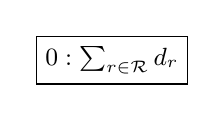
\begin{tikzpicture}
\small
\matrix[nodes={minimum size=6mm}] {
  \node[draw] {$0:\sum_{r\in\mathcal{R}}d_r$};\\
};
\end{tikzpicture}\\
\textbf{Side Effects:} none.\\
\textbf{Throws:} {\Tt{}SQLException\nwendquote} if database failure is encountered.\\
\bottomrule
\end{tabular}
\nwenddocs{}\nwbegincode{258}\sublabel{NW1Dx1yV-3ddWJ0-1}\nwmargintag{{\nwtagstyle{}\subpageref{NW1Dx1yV-3ddWJ0-1}}}\moddef{Read: DBQueryMetricRequestDistanceBaseTotal(0)~{\nwtagstyle{}\subpageref{NW1Dx1yV-3ddWJ0-1}}}\endmoddef\nwstartdeflinemarkup\nwusesondefline{\\{NW46kjAM-Oyob-1}}\nwenddeflinemarkup
int[] \nwlinkedidentc{DBQueryMetricRequestDistanceBaseTotal}{NW1Dx1yV-3ddWJ0-1}() throws SQLException \{
  // try (\LA{}Open \code{}conn\edoc{}~{\nwtagstyle{}\subpageref{NW1ODIS0-JT1v9-1}}\RA{}) \{
  //   return \nwlinkedidentc{PSQuery}{NW1ODIS0-yHOIP-1}(conn, "\nwlinkedidentc{S111}{NW1ODIS0-3WIudP-1}", 1);
  // \} catch (SQLException e) \{
  //   throw e;
  // \}
  return new int[] \{ this.sum_distance_base_requests \};
\}
\nwindexdefn{\nwixident{DBQueryMetricRequestDistanceBaseTotal}}{DBQueryMetricRequestDistanceBaseTotal}{NW1Dx1yV-3ddWJ0-1}\eatline
\nwused{\\{NW46kjAM-Oyob-1}}\nwidentdefs{\\{{\nwixident{DBQueryMetricRequestDistanceBaseTotal}}{DBQueryMetricRequestDistanceBaseTotal}}}\nwidentuses{\\{{\nwixident{PSQuery}}{PSQuery}}\\{{\nwixident{S111}}{S111}}}\nwindexuse{\nwixident{PSQuery}}{PSQuery}{NW1Dx1yV-3ddWJ0-1}\nwindexuse{\nwixident{S111}}{S111}{NW1Dx1yV-3ddWJ0-1}\nwendcode{}\nwbegindocs{259}\begin{tabular}{p{\textwidth}}
\toprule
\rowcolor{TableTitle}
Method \textcolor{blue}{{\Tt{}\nwlinkedidentq{queryMetricRequestDistanceBaseTotal}{NW1Dx1yV-v7TDa-1}\nwendquote}}(0) wraps {\Tt{}\nwlinkedidentq{DBQueryMetricRequestDistanceBaseTotal}{NW1Dx1yV-3ddWJ0-1}\nwendquote}(0).\\
\bottomrule
\end{tabular}
\nwenddocs{}\nwbegincode{260}\sublabel{NW1Dx1yV-v7TDa-1}\nwmargintag{{\nwtagstyle{}\subpageref{NW1Dx1yV-v7TDa-1}}}\moddef{Read: queryMetricRequestDistanceBaseTotal(0)~{\nwtagstyle{}\subpageref{NW1Dx1yV-v7TDa-1}}}\endmoddef\nwstartdeflinemarkup\nwusesondefline{\\{NW3hMOhb-2u8vSA-1}}\nwenddeflinemarkup
int[] \nwlinkedidentc{queryMetricRequestDistanceBaseTotal}{NW1Dx1yV-v7TDa-1}() throws SQLException \{
  int[] output = storage.\nwlinkedidentc{DBQueryMetricRequestDistanceBaseTotal}{NW1Dx1yV-3ddWJ0-1}();
  return output;
\}
\nwindexdefn{\nwixident{queryMetricRequestDistanceBaseTotal}}{queryMetricRequestDistanceBaseTotal}{NW1Dx1yV-v7TDa-1}\eatline
\nwused{\\{NW3hMOhb-2u8vSA-1}}\nwidentdefs{\\{{\nwixident{queryMetricRequestDistanceBaseTotal}}{queryMetricRequestDistanceBaseTotal}}}\nwidentuses{\\{{\nwixident{DBQueryMetricRequestDistanceBaseTotal}}{DBQueryMetricRequestDistanceBaseTotal}}}\nwindexuse{\nwixident{DBQueryMetricRequestDistanceBaseTotal}}{DBQueryMetricRequestDistanceBaseTotal}{NW1Dx1yV-v7TDa-1}\nwendcode{}\nwbegindocs{261}\nwdocspar
\subsubsection{\texttt{DBQueryMetricRequestDistanceBaseUnassignedTotal}(1)}
\begin{tabular}{p{\textwidth}}
\toprule
\rowcolor{TableTitle}
Method \textcolor{blue}{{\Tt{}\nwlinkedidentq{DBQueryMetricRequestDistanceBaseUnassignedTotal}{NW1Dx1yV-42edyi-1}\nwendquote}}(1) returns the
base distance of all the unassigned requests.
A {\Tt{}SQLException\nwendquote} is thrown in case of database failure.\\
\midrule
\textbf{Parameters:} none.\\
\textbf{Returns:} results of the query flattened into an integer array,
or {\Tt{}null\nwendquote} if no results.

\begin{tikzpicture}
\small
\matrix[nodes={minimum size=6mm}] {
  \node[draw] {$0:\sum_{r\in R^{ko}(\mathcal{X},H)}d_r$};\\
};
\end{tikzpicture}

where $H$ is the time horizon.\\
\textbf{Side Effects:} none.\\
\textbf{Throws:} {\Tt{}SQLException\nwendquote} if database failure is encountered.\\
\bottomrule
\end{tabular}
\nwenddocs{}\nwbegincode{262}\sublabel{NW1Dx1yV-42edyi-1}\nwmargintag{{\nwtagstyle{}\subpageref{NW1Dx1yV-42edyi-1}}}\moddef{Read: DBQueryMetricRequestDistanceBaseUnassignedTotal(1)~{\nwtagstyle{}\subpageref{NW1Dx1yV-42edyi-1}}}\endmoddef\nwstartdeflinemarkup\nwusesondefline{\\{NW46kjAM-Oyob-1}}\nwenddeflinemarkup
int[] \nwlinkedidentc{DBQueryMetricRequestDistanceBaseUnassignedTotal}{NW1Dx1yV-42edyi-1}(boolean flag_usecache) throws SQLException \{
  if (flag_usecache) \{
    return new int[] \{ this.sum_distance_unassigned \};
  \} else \{
    try (\LA{}Open \code{}conn\edoc{}~{\nwtagstyle{}\subpageref{NW1ODIS0-JT1v9-1}}\RA{}) \{
      return \nwlinkedidentc{PSQuery}{NW1ODIS0-yHOIP-1}(conn, "\nwlinkedidentc{S138}{NW1ODIS0-nWs2N-1}", 1);
    \} catch (SQLException e) \{
      throw e;
    \}
  \}
\}
\nwindexdefn{\nwixident{DBQueryMetricRequestDistanceBaseUnassignedTotal}}{DBQueryMetricRequestDistanceBaseUnassignedTotal}{NW1Dx1yV-42edyi-1}\eatline
\nwused{\\{NW46kjAM-Oyob-1}}\nwidentdefs{\\{{\nwixident{DBQueryMetricRequestDistanceBaseUnassignedTotal}}{DBQueryMetricRequestDistanceBaseUnassignedTotal}}}\nwidentuses{\\{{\nwixident{PSQuery}}{PSQuery}}\\{{\nwixident{S138}}{S138}}}\nwindexuse{\nwixident{PSQuery}}{PSQuery}{NW1Dx1yV-42edyi-1}\nwindexuse{\nwixident{S138}}{S138}{NW1Dx1yV-42edyi-1}\nwendcode{}\nwbegindocs{263}\begin{tabular}{p{\textwidth}}
\toprule
\rowcolor{TableTitle}
Method \textcolor{blue}{{\Tt{}\nwlinkedidentq{DBQueryMetricRequestDistanceBaseUnassignedTotal}{NW1Dx1yV-42edyi-1}\nwendquote}}(0)
calls {\Tt{}\nwlinkedidentq{DBQueryMetricRequestDistanceBaseUnassignedTotal}{NW1Dx1yV-42edyi-1}\nwendquote}(1)
with a default parameter.\\
\bottomrule
\end{tabular}
\nwenddocs{}\nwbegincode{264}\sublabel{NW1Dx1yV-421s5A-1}\nwmargintag{{\nwtagstyle{}\subpageref{NW1Dx1yV-421s5A-1}}}\moddef{Read: DBQueryMetricRequestDistanceBaseUnassignedTotal(0)~{\nwtagstyle{}\subpageref{NW1Dx1yV-421s5A-1}}}\endmoddef\nwstartdeflinemarkup\nwusesondefline{\\{NW46kjAM-Oyob-2}}\nwenddeflinemarkup
int[] \nwlinkedidentc{DBQueryMetricRequestDistanceBaseUnassignedTotal}{NW1Dx1yV-42edyi-1}() throws SQLException \{
  return \nwlinkedidentc{DBQueryMetricRequestDistanceBaseUnassignedTotal}{NW1Dx1yV-42edyi-1}(true);
\}
\nwused{\\{NW46kjAM-Oyob-2}}\nwidentuses{\\{{\nwixident{DBQueryMetricRequestDistanceBaseUnassignedTotal}}{DBQueryMetricRequestDistanceBaseUnassignedTotal}}}\nwindexuse{\nwixident{DBQueryMetricRequestDistanceBaseUnassignedTotal}}{DBQueryMetricRequestDistanceBaseUnassignedTotal}{NW1Dx1yV-421s5A-1}\nwendcode{}\nwbegindocs{265}\nwdocspar
\noindent
\begin{tabular}{p{\textwidth}}
\toprule
\rowcolor{TableTitle}
Method \textcolor{blue}{{\Tt{}\nwlinkedidentq{queryMetricRequestDistanceBaseUnassignedTotal}{NW1Dx1yV-4H96yt-1}\nwendquote}}(1) wraps {\Tt{}\nwlinkedidentq{DBQueryMetricRequestDistanceBaseUnassignedTotal}{NW1Dx1yV-42edyi-1}\nwendquote}(1).\\
\bottomrule
\end{tabular}
\nwenddocs{}\nwbegincode{266}\sublabel{NW1Dx1yV-4H96yt-1}\nwmargintag{{\nwtagstyle{}\subpageref{NW1Dx1yV-4H96yt-1}}}\moddef{Read: queryMetricRequestDistanceBaseUnassignedTotal(1)~{\nwtagstyle{}\subpageref{NW1Dx1yV-4H96yt-1}}}\endmoddef\nwstartdeflinemarkup\nwusesondefline{\\{NW3hMOhb-2u8vSA-1}}\nwenddeflinemarkup
int[] \nwlinkedidentc{queryMetricRequestDistanceBaseUnassignedTotal}{NW1Dx1yV-4H96yt-1}(boolean flag_usecache) throws SQLException \{
  int[] output = storage.\nwlinkedidentc{DBQueryMetricRequestDistanceBaseUnassignedTotal}{NW1Dx1yV-42edyi-1}(flag_usecache);
  return output;
\}
\nwindexdefn{\nwixident{queryMetricRequestDistanceBaseUnassignedTotal}}{queryMetricRequestDistanceBaseUnassignedTotal}{NW1Dx1yV-4H96yt-1}\eatline
\nwused{\\{NW3hMOhb-2u8vSA-1}}\nwidentdefs{\\{{\nwixident{queryMetricRequestDistanceBaseUnassignedTotal}}{queryMetricRequestDistanceBaseUnassignedTotal}}}\nwidentuses{\\{{\nwixident{DBQueryMetricRequestDistanceBaseUnassignedTotal}}{DBQueryMetricRequestDistanceBaseUnassignedTotal}}}\nwindexuse{\nwixident{DBQueryMetricRequestDistanceBaseUnassignedTotal}}{DBQueryMetricRequestDistanceBaseUnassignedTotal}{NW1Dx1yV-4H96yt-1}\nwendcode{}\nwbegindocs{267}\begin{tabular}{p{\textwidth}}
\toprule
\rowcolor{TableTitle}
Method \textcolor{blue}{{\Tt{}\nwlinkedidentq{queryMetricRequestDistanceBaseUnassignedTotal}{NW1Dx1yV-4H96yt-1}\nwendquote}}(0)
calls {\Tt{}\nwlinkedidentq{queryMetricRequestDistanceBaseUnassignedTotal}{NW1Dx1yV-4H96yt-1}\nwendquote}(1)
with a default parameter.\\
\bottomrule
\end{tabular}
\nwenddocs{}\nwbegincode{268}\sublabel{NW1Dx1yV-4H3t3H-1}\nwmargintag{{\nwtagstyle{}\subpageref{NW1Dx1yV-4H3t3H-1}}}\moddef{Read: queryMetricRequestDistanceBaseUnassignedTotal(0)~{\nwtagstyle{}\subpageref{NW1Dx1yV-4H3t3H-1}}}\endmoddef\nwstartdeflinemarkup\nwusesondefline{\\{NW3hMOhb-2u8vSA-2}}\nwenddeflinemarkup
int[] \nwlinkedidentc{queryMetricRequestDistanceBaseUnassignedTotal}{NW1Dx1yV-4H96yt-1}() throws SQLException \{
  return \nwlinkedidentc{queryMetricRequestDistanceBaseUnassignedTotal}{NW1Dx1yV-4H96yt-1}(true);
\}
\nwused{\\{NW3hMOhb-2u8vSA-2}}\nwidentuses{\\{{\nwixident{queryMetricRequestDistanceBaseUnassignedTotal}}{queryMetricRequestDistanceBaseUnassignedTotal}}}\nwindexuse{\nwixident{queryMetricRequestDistanceBaseUnassignedTotal}}{queryMetricRequestDistanceBaseUnassignedTotal}{NW1Dx1yV-4H3t3H-1}\nwendcode{}\nwbegindocs{269}\nwdocspar

\subsubsection{\texttt{DBQueryMetricRequestDistanceBaseUnassignedRunning}(0)}
\nwenddocs{}\nwbegincode{270}\sublabel{NW1Dx1yV-4UUzlW-1}\nwmargintag{{\nwtagstyle{}\subpageref{NW1Dx1yV-4UUzlW-1}}}\moddef{Read: DBQueryMetricRequestDistanceBaseUnassignedRunning(0)~{\nwtagstyle{}\subpageref{NW1Dx1yV-4UUzlW-1}}}\endmoddef\nwstartdeflinemarkup\nwusesondefline{\\{NW46kjAM-Oyob-1}}\nwenddeflinemarkup
int[] \nwlinkedidentc{DBQueryMetricRequestDistanceBaseUnassignedRunning}{NW1Dx1yV-4UUzlW-1}() throws SQLException \{
  int[] output = new int[] \{ \};
  // ...
  return output;
\}
\nwindexdefn{\nwixident{DBQueryMetricRequestDistanceBaseUnassignedRunning}}{DBQueryMetricRequestDistanceBaseUnassignedRunning}{NW1Dx1yV-4UUzlW-1}\eatline
\nwused{\\{NW46kjAM-Oyob-1}}\nwidentdefs{\\{{\nwixident{DBQueryMetricRequestDistanceBaseUnassignedRunning}}{DBQueryMetricRequestDistanceBaseUnassignedRunning}}}\nwendcode{}\nwbegincode{271}\sublabel{NW1Dx1yV-2XxVoJ-1}\nwmargintag{{\nwtagstyle{}\subpageref{NW1Dx1yV-2XxVoJ-1}}}\moddef{Read: queryMetricRequestDistanceBaseUnassignedRunning(0)~{\nwtagstyle{}\subpageref{NW1Dx1yV-2XxVoJ-1}}}\endmoddef\nwstartdeflinemarkup\nwusesondefline{\\{NW3hMOhb-2u8vSA-1}}\nwenddeflinemarkup
int[] queryMetricRequestDistanceBaseUnassignedRunning()
throws SQLException, \nwlinkedidentc{UserNotFoundException}{NW1ODIS0-15irq2-1} \{
  int[] output = new int[] \{ 0 \};
  for (int rid : this.lu_rseen.keySet()) \{
    if (this.storage.\nwlinkedidentc{DBQueryRequestIsAssigned}{NW1Dx1yV-1Ypj7S-1}(rid, true).length == 0) \{
      output[0] += this.storage.\nwlinkedidentc{DBQueryUser}{NW1Dx1yV-8IJdE-1}(rid)[6];
    \}
  \}
  return output;
\}
\nwused{\\{NW3hMOhb-2u8vSA-1}}\nwidentuses{\\{{\nwixident{DBQueryRequestIsAssigned}}{DBQueryRequestIsAssigned}}\\{{\nwixident{DBQueryUser}}{DBQueryUser}}\\{{\nwixident{UserNotFoundException}}{UserNotFoundException}}}\nwindexuse{\nwixident{DBQueryRequestIsAssigned}}{DBQueryRequestIsAssigned}{NW1Dx1yV-2XxVoJ-1}\nwindexuse{\nwixident{DBQueryUser}}{DBQueryUser}{NW1Dx1yV-2XxVoJ-1}\nwindexuse{\nwixident{UserNotFoundException}}{UserNotFoundException}{NW1Dx1yV-2XxVoJ-1}\nwendcode{}\nwbegindocs{272}\nwdocspar

\subsubsection{\texttt{DBQueryMetricRequestDistanceDetourTotal}(1)}
\begin{tabular}{p{\textwidth}}
\toprule
\rowcolor{TableTitle}
Method \textcolor{blue}{{\Tt{}\nwlinkedidentq{DBQueryMetricRequestDistanceDetourTotal}{NW1Dx1yV-2z9Wsm-1}\nwendquote}}(1) returns the
total detour distance of all requests.
A {\Tt{}SQLException\nwendquote} is thrown in case of database failure.\\
\midrule
\textbf{Parameters:} none.\\
\textbf{Returns:} results of the query flattened into an integer array,
or {\Tt{}null\nwendquote} if no results.

\begin{tikzpicture}
\small
\matrix[nodes={minimum size=6mm}] {
  \node[draw] {$0:\sum_{r\in\mathcal{R}}D^\textrm{detour}(\mathcal{X},r)$};\\
};
\end{tikzpicture}\\
\textbf{Side Effects:} none.\\
\textbf{Throws:} {\Tt{}SQLException\nwendquote} if database failure is encountered.\\
\bottomrule
\end{tabular}
\nwenddocs{}\nwbegincode{273}\sublabel{NW1Dx1yV-2z9Wsm-1}\nwmargintag{{\nwtagstyle{}\subpageref{NW1Dx1yV-2z9Wsm-1}}}\moddef{Read: DBQueryMetricRequestDistanceDetourTotal(1)~{\nwtagstyle{}\subpageref{NW1Dx1yV-2z9Wsm-1}}}\endmoddef\nwstartdeflinemarkup\nwusesondefline{\\{NW46kjAM-Oyob-1}}\nwenddeflinemarkup
int[] \nwlinkedidentc{DBQueryMetricRequestDistanceDetourTotal}{NW1Dx1yV-2z9Wsm-1}(boolean flag_usecache) throws SQLException \{
  if (flag_usecache) \{
    final int[] output = new int[] \{ 0 \};
    this.distance_requests_transit.forEach((rid, val) ->
      output[0] += (val - this.lu_users.get(rid)[6])
    );
    return output;
  \} else \{
    try (\LA{}Open \code{}conn\edoc{}~{\nwtagstyle{}\subpageref{NW1ODIS0-JT1v9-1}}\RA{}) \{
      return \nwlinkedidentc{PSQuery}{NW1ODIS0-yHOIP-1}(conn, "\nwlinkedidentc{S113}{NW1ODIS0-3Q3jlz-1}", 1);
    \} catch (SQLException e) \{
      throw e;
    \}
  \}
\}
\nwindexdefn{\nwixident{DBQueryMetricRequestDistanceDetourTotal}}{DBQueryMetricRequestDistanceDetourTotal}{NW1Dx1yV-2z9Wsm-1}\eatline
\nwused{\\{NW46kjAM-Oyob-1}}\nwidentdefs{\\{{\nwixident{DBQueryMetricRequestDistanceDetourTotal}}{DBQueryMetricRequestDistanceDetourTotal}}}\nwidentuses{\\{{\nwixident{PSQuery}}{PSQuery}}\\{{\nwixident{S113}}{S113}}}\nwindexuse{\nwixident{PSQuery}}{PSQuery}{NW1Dx1yV-2z9Wsm-1}\nwindexuse{\nwixident{S113}}{S113}{NW1Dx1yV-2z9Wsm-1}\nwendcode{}\nwbegindocs{274}\begin{tabular}{p{\textwidth}}
\toprule
\rowcolor{TableTitle}
Method \textcolor{blue}{{\Tt{}\nwlinkedidentq{DBQueryMetricRequestDistanceDetourTotal}{NW1Dx1yV-2z9Wsm-1}\nwendquote}}(0) calls {\Tt{}\nwlinkedidentq{DBQueryMetricRequestDistanceDetourTotal}{NW1Dx1yV-2z9Wsm-1}\nwendquote}(1)
with a default parameter.\\
\bottomrule
\end{tabular}
\nwenddocs{}\nwbegincode{275}\sublabel{NW1Dx1yV-3066Ie-1}\nwmargintag{{\nwtagstyle{}\subpageref{NW1Dx1yV-3066Ie-1}}}\moddef{Read: DBQueryMetricRequestDistanceDetourTotal(0)~{\nwtagstyle{}\subpageref{NW1Dx1yV-3066Ie-1}}}\endmoddef\nwstartdeflinemarkup\nwusesondefline{\\{NW46kjAM-Oyob-2}}\nwenddeflinemarkup
int[] \nwlinkedidentc{DBQueryMetricRequestDistanceDetourTotal}{NW1Dx1yV-2z9Wsm-1}() throws SQLException \{
  return \nwlinkedidentc{DBQueryMetricRequestDistanceDetourTotal}{NW1Dx1yV-2z9Wsm-1}(true);
\}
\nwused{\\{NW46kjAM-Oyob-2}}\nwidentuses{\\{{\nwixident{DBQueryMetricRequestDistanceDetourTotal}}{DBQueryMetricRequestDistanceDetourTotal}}}\nwindexuse{\nwixident{DBQueryMetricRequestDistanceDetourTotal}}{DBQueryMetricRequestDistanceDetourTotal}{NW1Dx1yV-3066Ie-1}\nwendcode{}\nwbegindocs{276}\nwdocspar
\noindent
\begin{tabular}{p{\textwidth}}
\toprule
\rowcolor{TableTitle}
Method \textcolor{blue}{{\Tt{}\nwlinkedidentq{queryMetricRequestDistanceDetourTotal}{NW1Dx1yV-1HM4JE-1}\nwendquote}}(1) wraps {\Tt{}\nwlinkedidentq{DBQueryMetricRequestDistanceDetourTotal}{NW1Dx1yV-2z9Wsm-1}\nwendquote}(1).\\
\bottomrule
\end{tabular}
\nwenddocs{}\nwbegincode{277}\sublabel{NW1Dx1yV-1HM4JE-1}\nwmargintag{{\nwtagstyle{}\subpageref{NW1Dx1yV-1HM4JE-1}}}\moddef{Read: queryMetricRequestDistanceDetourTotal(1)~{\nwtagstyle{}\subpageref{NW1Dx1yV-1HM4JE-1}}}\endmoddef\nwstartdeflinemarkup\nwusesondefline{\\{NW3hMOhb-2u8vSA-1}}\nwenddeflinemarkup
int[] \nwlinkedidentc{queryMetricRequestDistanceDetourTotal}{NW1Dx1yV-1HM4JE-1}(boolean flag_usecache) throws SQLException \{
  int[] output = storage.\nwlinkedidentc{DBQueryMetricRequestDistanceDetourTotal}{NW1Dx1yV-2z9Wsm-1}(flag_usecache);
  return output;
\}
\nwindexdefn{\nwixident{queryMetricRequestDistanceDetourTotal}}{queryMetricRequestDistanceDetourTotal}{NW1Dx1yV-1HM4JE-1}\eatline
\nwused{\\{NW3hMOhb-2u8vSA-1}}\nwidentdefs{\\{{\nwixident{queryMetricRequestDistanceDetourTotal}}{queryMetricRequestDistanceDetourTotal}}}\nwidentuses{\\{{\nwixident{DBQueryMetricRequestDistanceDetourTotal}}{DBQueryMetricRequestDistanceDetourTotal}}}\nwindexuse{\nwixident{DBQueryMetricRequestDistanceDetourTotal}}{DBQueryMetricRequestDistanceDetourTotal}{NW1Dx1yV-1HM4JE-1}\nwendcode{}\nwbegindocs{278}\begin{tabular}{p{\textwidth}}
\toprule
\rowcolor{TableTitle}
Method \textcolor{blue}{{\Tt{}\nwlinkedidentq{queryMetricRequestDistanceDetourTotal}{NW1Dx1yV-1HM4JE-1}\nwendquote}}(0) calls {\Tt{}\nwlinkedidentq{queryMetricRequestDistanceDetourTotal}{NW1Dx1yV-1HM4JE-1}\nwendquote}(1)
with a default parameter.\\
\bottomrule
\end{tabular}
\nwenddocs{}\nwbegincode{279}\sublabel{NW1Dx1yV-1GQ2zQ-1}\nwmargintag{{\nwtagstyle{}\subpageref{NW1Dx1yV-1GQ2zQ-1}}}\moddef{Read: queryMetricRequestDistanceDetourTotal(0)~{\nwtagstyle{}\subpageref{NW1Dx1yV-1GQ2zQ-1}}}\endmoddef\nwstartdeflinemarkup\nwusesondefline{\\{NW3hMOhb-2u8vSA-2}}\nwenddeflinemarkup
int[] \nwlinkedidentc{queryMetricRequestDistanceDetourTotal}{NW1Dx1yV-1HM4JE-1}() throws SQLException \{
  return \nwlinkedidentc{queryMetricRequestDistanceDetourTotal}{NW1Dx1yV-1HM4JE-1}(true);
\}
\nwused{\\{NW3hMOhb-2u8vSA-2}}\nwidentuses{\\{{\nwixident{queryMetricRequestDistanceDetourTotal}}{queryMetricRequestDistanceDetourTotal}}}\nwindexuse{\nwixident{queryMetricRequestDistanceDetourTotal}}{queryMetricRequestDistanceDetourTotal}{NW1Dx1yV-1GQ2zQ-1}\nwendcode{}\nwbegindocs{280}\nwdocspar

\subsubsection{\texttt{DBQueryMetricRequestDistanceTransitTotal}(1)}
\begin{tabular}{p{\textwidth}}
\toprule
\rowcolor{TableTitle}
Method \textcolor{blue}{{\Tt{}\nwlinkedidentq{DBQueryMetricRequestDistanceTransitTotal}{NW1Dx1yV-Y8OUv-1}\nwendquote}}(1) returns the
total transit distance of all requests.
A {\Tt{}SQLException\nwendquote} is thrown in case of database failure.\\
\midrule
\textbf{Parameters:} none.\\
\textbf{Returns:} results of the query flattened into an integer array,
or {\Tt{}null\nwendquote} if no results.

\begin{tikzpicture}
\small
\matrix[nodes={minimum size=6mm}] {
  \node[draw] {$0:\sum_{r\in\mathcal{R}}D^\textrm{transit}(\mathcal{X},r)$};\\
};
\end{tikzpicture}\\
\textbf{Side Effects:} none.\\
\textbf{Throws:} {\Tt{}SQLException\nwendquote} if database failure is encountered.\\
\bottomrule
\end{tabular}
\nwenddocs{}\nwbegincode{281}\sublabel{NW1Dx1yV-Y8OUv-1}\nwmargintag{{\nwtagstyle{}\subpageref{NW1Dx1yV-Y8OUv-1}}}\moddef{Read: DBQueryMetricRequestDistanceTransitTotal(1)~{\nwtagstyle{}\subpageref{NW1Dx1yV-Y8OUv-1}}}\endmoddef\nwstartdeflinemarkup\nwusesondefline{\\{NW46kjAM-Oyob-1}}\nwenddeflinemarkup
int[] \nwlinkedidentc{DBQueryMetricRequestDistanceTransitTotal}{NW1Dx1yV-Y8OUv-1}(boolean flag_usecache) throws SQLException \{
  if (flag_usecache) \{
    final int[] output = new int[] \{ 0 \};
    this.distance_requests_transit.forEach((rid, val) -> output[0] += val);
    return output;
  \} else \{
    try (\LA{}Open \code{}conn\edoc{}~{\nwtagstyle{}\subpageref{NW1ODIS0-JT1v9-1}}\RA{}) \{
      return \nwlinkedidentc{PSQuery}{NW1ODIS0-yHOIP-1}(conn, "\nwlinkedidentc{S115}{NW1ODIS0-4dHRF5-1}", 1);
    \} catch (SQLException e) \{
      throw e;
    \}
  \}
\}
\nwindexdefn{\nwixident{DBQueryMetricRequestDistanceTransitTotal}}{DBQueryMetricRequestDistanceTransitTotal}{NW1Dx1yV-Y8OUv-1}\eatline
\nwused{\\{NW46kjAM-Oyob-1}}\nwidentdefs{\\{{\nwixident{DBQueryMetricRequestDistanceTransitTotal}}{DBQueryMetricRequestDistanceTransitTotal}}}\nwidentuses{\\{{\nwixident{PSQuery}}{PSQuery}}\\{{\nwixident{S115}}{S115}}}\nwindexuse{\nwixident{PSQuery}}{PSQuery}{NW1Dx1yV-Y8OUv-1}\nwindexuse{\nwixident{S115}}{S115}{NW1Dx1yV-Y8OUv-1}\nwendcode{}\nwbegindocs{282}\begin{tabular}{p{\textwidth}}
\toprule
\rowcolor{TableTitle}
Method \textcolor{blue}{{\Tt{}\nwlinkedidentq{DBQueryMetricRequestDistanceTransitTotal}{NW1Dx1yV-Y8OUv-1}\nwendquote}}(0) calls {\Tt{}\nwlinkedidentq{DBQueryMetricRequestDistanceTransitTotal}{NW1Dx1yV-Y8OUv-1}\nwendquote}(1)
with a default parameter.\\
\bottomrule
\end{tabular}
\nwenddocs{}\nwbegincode{283}\sublabel{NW1Dx1yV-Z4xun-1}\nwmargintag{{\nwtagstyle{}\subpageref{NW1Dx1yV-Z4xun-1}}}\moddef{Read: DBQueryMetricRequestDistanceTransitTotal(0)~{\nwtagstyle{}\subpageref{NW1Dx1yV-Z4xun-1}}}\endmoddef\nwstartdeflinemarkup\nwusesondefline{\\{NW46kjAM-Oyob-2}}\nwenddeflinemarkup
int[] \nwlinkedidentc{DBQueryMetricRequestDistanceTransitTotal}{NW1Dx1yV-Y8OUv-1}() throws SQLException \{
  return \nwlinkedidentc{DBQueryMetricRequestDistanceTransitTotal}{NW1Dx1yV-Y8OUv-1}(true);
\}
\nwused{\\{NW46kjAM-Oyob-2}}\nwidentuses{\\{{\nwixident{DBQueryMetricRequestDistanceTransitTotal}}{DBQueryMetricRequestDistanceTransitTotal}}}\nwindexuse{\nwixident{DBQueryMetricRequestDistanceTransitTotal}}{DBQueryMetricRequestDistanceTransitTotal}{NW1Dx1yV-Z4xun-1}\nwendcode{}\nwbegindocs{284}\nwdocspar
\noindent
\begin{tabular}{p{\textwidth}}
\toprule
\rowcolor{TableTitle}
Method \textcolor{blue}{{\Tt{}\nwlinkedidentq{queryMetricRequestDistanceTransitTotal}{NW1Dx1yV-l3AND-1}\nwendquote}}(1) wraps {\Tt{}\nwlinkedidentq{DBQueryMetricRequestDistanceTransitTotal}{NW1Dx1yV-Y8OUv-1}\nwendquote}(1).\\
\bottomrule
\end{tabular}
\nwenddocs{}\nwbegincode{285}\sublabel{NW1Dx1yV-l3AND-1}\nwmargintag{{\nwtagstyle{}\subpageref{NW1Dx1yV-l3AND-1}}}\moddef{Read: queryMetricRequestDistanceTransitTotal(1)~{\nwtagstyle{}\subpageref{NW1Dx1yV-l3AND-1}}}\endmoddef\nwstartdeflinemarkup\nwusesondefline{\\{NW3hMOhb-2u8vSA-1}}\nwenddeflinemarkup
int[] \nwlinkedidentc{queryMetricRequestDistanceTransitTotal}{NW1Dx1yV-l3AND-1}(boolean flag_usecache) throws SQLException \{
  int[] output = storage.\nwlinkedidentc{DBQueryMetricRequestDistanceTransitTotal}{NW1Dx1yV-Y8OUv-1}(flag_usecache);
  return output;
\}
\nwindexdefn{\nwixident{queryMetricRequestDistanceTransitTotal}}{queryMetricRequestDistanceTransitTotal}{NW1Dx1yV-l3AND-1}\eatline
\nwused{\\{NW3hMOhb-2u8vSA-1}}\nwidentdefs{\\{{\nwixident{queryMetricRequestDistanceTransitTotal}}{queryMetricRequestDistanceTransitTotal}}}\nwidentuses{\\{{\nwixident{DBQueryMetricRequestDistanceTransitTotal}}{DBQueryMetricRequestDistanceTransitTotal}}}\nwindexuse{\nwixident{DBQueryMetricRequestDistanceTransitTotal}}{DBQueryMetricRequestDistanceTransitTotal}{NW1Dx1yV-l3AND-1}\nwendcode{}\nwbegindocs{286}\begin{tabular}{p{\textwidth}}
\toprule
\rowcolor{TableTitle}
Method \textcolor{blue}{{\Tt{}\nwlinkedidentq{queryMetricRequestDistanceTransitTotal}{NW1Dx1yV-l3AND-1}\nwendquote}}(0) calls {\Tt{}\nwlinkedidentq{queryMetricRequestDistanceTransitTotal}{NW1Dx1yV-l3AND-1}\nwendquote}(1)
with a default parameter.\\
\bottomrule
\end{tabular}
\nwenddocs{}\nwbegincode{287}\sublabel{NW1Dx1yV-l8wOt-1}\nwmargintag{{\nwtagstyle{}\subpageref{NW1Dx1yV-l8wOt-1}}}\moddef{Read: queryMetricRequestDistanceTransitTotal(0)~{\nwtagstyle{}\subpageref{NW1Dx1yV-l8wOt-1}}}\endmoddef\nwstartdeflinemarkup\nwusesondefline{\\{NW3hMOhb-2u8vSA-2}}\nwenddeflinemarkup
int[] \nwlinkedidentc{queryMetricRequestDistanceTransitTotal}{NW1Dx1yV-l3AND-1}() throws SQLException \{
  return \nwlinkedidentc{queryMetricRequestDistanceTransitTotal}{NW1Dx1yV-l3AND-1}(true);
\}
\nwused{\\{NW3hMOhb-2u8vSA-2}}\nwidentuses{\\{{\nwixident{queryMetricRequestDistanceTransitTotal}}{queryMetricRequestDistanceTransitTotal}}}\nwindexuse{\nwixident{queryMetricRequestDistanceTransitTotal}}{queryMetricRequestDistanceTransitTotal}{NW1Dx1yV-l8wOt-1}\nwendcode{}\nwbegindocs{288}\nwdocspar

\subsubsection{\texttt{DBQueryMetricRequestDurationPickupTotal}(1)}
\begin{tabular}{p{\textwidth}}
\toprule
\rowcolor{TableTitle}
Method \textcolor{blue}{{\Tt{}\nwlinkedidentq{DBQueryMetricRequestDurationPickupTotal}{NW1Dx1yV-29sr46-1}\nwendquote}}(1) returns the
total pickup delay of all requests.
A {\Tt{}SQLException\nwendquote} is thrown in case of database failure.\\
\midrule
\textbf{Parameters:} none.\\
\textbf{Returns:} results of the query flattened into an integer array,
or {\Tt{}null\nwendquote} if no results.

\begin{tikzpicture}
\small
\matrix[nodes={minimum size=6mm}] {
  \node[draw] {$0:\sum_{r\in\mathcal{R}}\delta^\textrm{pickup}(\mathcal{X},r)$};\\
};
\end{tikzpicture}\\
\textbf{Side Effects:} none.\\
\textbf{Throws:} {\Tt{}SQLException\nwendquote} if database failure is encountered.\\
\bottomrule
\end{tabular}
\nwenddocs{}\nwbegincode{289}\sublabel{NW1Dx1yV-29sr46-1}\nwmargintag{{\nwtagstyle{}\subpageref{NW1Dx1yV-29sr46-1}}}\moddef{Read: DBQueryMetricRequestDurationPickupTotal(1)~{\nwtagstyle{}\subpageref{NW1Dx1yV-29sr46-1}}}\endmoddef\nwstartdeflinemarkup\nwusesondefline{\\{NW46kjAM-Oyob-1}}\nwenddeflinemarkup
int[] \nwlinkedidentc{DBQueryMetricRequestDurationPickupTotal}{NW1Dx1yV-29sr46-1}(boolean flag_usecache) throws SQLException \{
  if (flag_usecache) \{
    final int[] output = new int[] \{ 0 \};
    this.duration_requests_pickup.forEach((rid, val) -> output[0] += val);
    return output;
  \} else \{
    try (\LA{}Open \code{}conn\edoc{}~{\nwtagstyle{}\subpageref{NW1ODIS0-JT1v9-1}}\RA{}) \{
      return \nwlinkedidentc{PSQuery}{NW1ODIS0-yHOIP-1}(conn, "\nwlinkedidentc{S119}{NW1ODIS0-454m4J-1}", 1);
    \} catch (SQLException e) \{
      throw e;
    \}
  \}
\}
\nwindexdefn{\nwixident{DBQueryMetricRequestDurationPickupTotal}}{DBQueryMetricRequestDurationPickupTotal}{NW1Dx1yV-29sr46-1}\eatline
\nwused{\\{NW46kjAM-Oyob-1}}\nwidentdefs{\\{{\nwixident{DBQueryMetricRequestDurationPickupTotal}}{DBQueryMetricRequestDurationPickupTotal}}}\nwidentuses{\\{{\nwixident{PSQuery}}{PSQuery}}\\{{\nwixident{S119}}{S119}}}\nwindexuse{\nwixident{PSQuery}}{PSQuery}{NW1Dx1yV-29sr46-1}\nwindexuse{\nwixident{S119}}{S119}{NW1Dx1yV-29sr46-1}\nwendcode{}\nwbegindocs{290}\begin{tabular}{p{\textwidth}}
\toprule
\rowcolor{TableTitle}
Method \textcolor{blue}{{\Tt{}\nwlinkedidentq{DBQueryMetricRequestDurationPickupTotal}{NW1Dx1yV-29sr46-1}\nwendquote}}(0) calls {\Tt{}\nwlinkedidentq{DBQueryMetricRequestDurationPickupTotal}{NW1Dx1yV-29sr46-1}\nwendquote}(1)
with a default parameter.\\
\bottomrule
\end{tabular}
\nwenddocs{}\nwbegincode{291}\sublabel{NW1Dx1yV-28z28Y-1}\nwmargintag{{\nwtagstyle{}\subpageref{NW1Dx1yV-28z28Y-1}}}\moddef{Read: DBQueryMetricRequestDurationPickupTotal(0)~{\nwtagstyle{}\subpageref{NW1Dx1yV-28z28Y-1}}}\endmoddef\nwstartdeflinemarkup\nwusesondefline{\\{NW46kjAM-Oyob-2}}\nwenddeflinemarkup
int[] \nwlinkedidentc{DBQueryMetricRequestDurationPickupTotal}{NW1Dx1yV-29sr46-1}() throws SQLException \{
  return \nwlinkedidentc{DBQueryMetricRequestDurationPickupTotal}{NW1Dx1yV-29sr46-1}(true);
\}
\nwused{\\{NW46kjAM-Oyob-2}}\nwidentuses{\\{{\nwixident{DBQueryMetricRequestDurationPickupTotal}}{DBQueryMetricRequestDurationPickupTotal}}}\nwindexuse{\nwixident{DBQueryMetricRequestDurationPickupTotal}}{DBQueryMetricRequestDurationPickupTotal}{NW1Dx1yV-28z28Y-1}\nwendcode{}\nwbegindocs{292}\nwdocspar
\noindent
\begin{tabular}{p{\textwidth}}
\toprule
\rowcolor{TableTitle}
Method \textcolor{blue}{{\Tt{}\nwlinkedidentq{queryMetricRequestDurationPickupTotal}{NW1Dx1yV-2h26ru-1}\nwendquote}}(1) wraps {\Tt{}\nwlinkedidentq{DBQueryMetricRequestDurationPickupTotal}{NW1Dx1yV-29sr46-1}\nwendquote}(1).\\
\bottomrule
\end{tabular}
\nwenddocs{}\nwbegincode{293}\sublabel{NW1Dx1yV-2h26ru-1}\nwmargintag{{\nwtagstyle{}\subpageref{NW1Dx1yV-2h26ru-1}}}\moddef{Read: queryMetricRequestDurationPickupTotal(1)~{\nwtagstyle{}\subpageref{NW1Dx1yV-2h26ru-1}}}\endmoddef\nwstartdeflinemarkup\nwusesondefline{\\{NW3hMOhb-2u8vSA-1}}\nwenddeflinemarkup
int[] \nwlinkedidentc{queryMetricRequestDurationPickupTotal}{NW1Dx1yV-2h26ru-1}(boolean flag_usecache) throws SQLException \{
  int[] output = storage.\nwlinkedidentc{DBQueryMetricRequestDurationPickupTotal}{NW1Dx1yV-29sr46-1}(flag_usecache);
  return output;
\}
\nwindexdefn{\nwixident{queryMetricRequestDurationPickupTotal}}{queryMetricRequestDurationPickupTotal}{NW1Dx1yV-2h26ru-1}\eatline
\nwused{\\{NW3hMOhb-2u8vSA-1}}\nwidentdefs{\\{{\nwixident{queryMetricRequestDurationPickupTotal}}{queryMetricRequestDurationPickupTotal}}}\nwidentuses{\\{{\nwixident{DBQueryMetricRequestDurationPickupTotal}}{DBQueryMetricRequestDurationPickupTotal}}}\nwindexuse{\nwixident{DBQueryMetricRequestDurationPickupTotal}}{DBQueryMetricRequestDurationPickupTotal}{NW1Dx1yV-2h26ru-1}\nwendcode{}\nwbegindocs{294}\begin{tabular}{p{\textwidth}}
\toprule
\rowcolor{TableTitle}
Method \textcolor{blue}{{\Tt{}\nwlinkedidentq{queryMetricRequestDurationPickupTotal}{NW1Dx1yV-2h26ru-1}\nwendquote}}(0) calls {\Tt{}\nwlinkedidentq{queryMetricRequestDurationPickupTotal}{NW1Dx1yV-2h26ru-1}\nwendquote}(1)
with a default parameter.\\
\bottomrule
\end{tabular}
\nwenddocs{}\nwbegincode{295}\sublabel{NW1Dx1yV-2hwTtW-1}\nwmargintag{{\nwtagstyle{}\subpageref{NW1Dx1yV-2hwTtW-1}}}\moddef{Read: queryMetricRequestDurationPickupTotal(0)~{\nwtagstyle{}\subpageref{NW1Dx1yV-2hwTtW-1}}}\endmoddef\nwstartdeflinemarkup\nwusesondefline{\\{NW3hMOhb-2u8vSA-2}}\nwenddeflinemarkup
int[] \nwlinkedidentc{queryMetricRequestDurationPickupTotal}{NW1Dx1yV-2h26ru-1}() throws SQLException \{
  return \nwlinkedidentc{queryMetricRequestDurationPickupTotal}{NW1Dx1yV-2h26ru-1}(true);
\}
\nwused{\\{NW3hMOhb-2u8vSA-2}}\nwidentuses{\\{{\nwixident{queryMetricRequestDurationPickupTotal}}{queryMetricRequestDurationPickupTotal}}}\nwindexuse{\nwixident{queryMetricRequestDurationPickupTotal}}{queryMetricRequestDurationPickupTotal}{NW1Dx1yV-2hwTtW-1}\nwendcode{}\nwbegindocs{296}\nwdocspar

\subsubsection{\texttt{DBQueryMetricRequestDurationTransitTotal}(1)}
\begin{tabular}{p{\textwidth}}
\toprule
\rowcolor{TableTitle}
Method \textcolor{blue}{{\Tt{}\nwlinkedidentq{DBQueryMetricRequestDurationTransitTotal}{NW1Dx1yV-2RzFB3-1}\nwendquote}}(1) returns the
total transit duration of all requests.
A {\Tt{}SQLException\nwendquote} is thrown in case of database failure.\\
\midrule
\textbf{Parameters:} none.\\
\textbf{Returns:} results of the query flattened into an integer array,
or {\Tt{}null\nwendquote} if no results.

\begin{tikzpicture}
\small
\matrix[nodes={minimum size=6mm}] {
  \node[draw] {$0:\sum_{r\in\mathcal{R}}\delta^\textrm{transit}(\mathcal{X},r)$};\\
};
\end{tikzpicture}\\
\textbf{Side Effects:} none.\\
\textbf{Throws:} {\Tt{}SQLException\nwendquote} if database failure is encountered.\\
\bottomrule
\end{tabular}
\nwenddocs{}\nwbegincode{297}\sublabel{NW1Dx1yV-2RzFB3-1}\nwmargintag{{\nwtagstyle{}\subpageref{NW1Dx1yV-2RzFB3-1}}}\moddef{Read: DBQueryMetricRequestDurationTransitTotal(1)~{\nwtagstyle{}\subpageref{NW1Dx1yV-2RzFB3-1}}}\endmoddef\nwstartdeflinemarkup\nwusesondefline{\\{NW46kjAM-Oyob-1}}\nwenddeflinemarkup
int[] \nwlinkedidentc{DBQueryMetricRequestDurationTransitTotal}{NW1Dx1yV-2RzFB3-1}(boolean flag_usecache) throws SQLException \{
  if (flag_usecache) \{
    final int[] output = new int[] \{ 0 \};
    this.duration_requests_transit.forEach((rid, val) -> output[0] += val);
    return output;
  \} else \{
    try (\LA{}Open \code{}conn\edoc{}~{\nwtagstyle{}\subpageref{NW1ODIS0-JT1v9-1}}\RA{}) \{
      return \nwlinkedidentc{PSQuery}{NW1ODIS0-yHOIP-1}(conn, "\nwlinkedidentc{S121}{NW1ODIS0-3WtcfD-1}", 1);
    \} catch (SQLException e) \{
      throw e;
    \}
  \}
\}
\nwindexdefn{\nwixident{DBQueryMetricRequestDurationTransitTotal}}{DBQueryMetricRequestDurationTransitTotal}{NW1Dx1yV-2RzFB3-1}\eatline
\nwused{\\{NW46kjAM-Oyob-1}}\nwidentdefs{\\{{\nwixident{DBQueryMetricRequestDurationTransitTotal}}{DBQueryMetricRequestDurationTransitTotal}}}\nwidentuses{\\{{\nwixident{PSQuery}}{PSQuery}}\\{{\nwixident{S121}}{S121}}}\nwindexuse{\nwixident{PSQuery}}{PSQuery}{NW1Dx1yV-2RzFB3-1}\nwindexuse{\nwixident{S121}}{S121}{NW1Dx1yV-2RzFB3-1}\nwendcode{}\nwbegindocs{298}\begin{tabular}{p{\textwidth}}
\toprule
\rowcolor{TableTitle}
Method \textcolor{blue}{{\Tt{}\nwlinkedidentq{DBQueryMetricRequestDurationTransitTotal}{NW1Dx1yV-2RzFB3-1}\nwendquote}}(0) calls {\Tt{}\nwlinkedidentq{DBQueryMetricRequestDurationTransitTotal}{NW1Dx1yV-2RzFB3-1}\nwendquote}(1)
with a default parameter.\\
\bottomrule
\end{tabular}
\nwenddocs{}\nwbegincode{299}\sublabel{NW1Dx1yV-2RC1QH-1}\nwmargintag{{\nwtagstyle{}\subpageref{NW1Dx1yV-2RC1QH-1}}}\moddef{Read: DBQueryMetricRequestDurationTransitTotal(0)~{\nwtagstyle{}\subpageref{NW1Dx1yV-2RC1QH-1}}}\endmoddef\nwstartdeflinemarkup\nwusesondefline{\\{NW46kjAM-Oyob-2}}\nwenddeflinemarkup
int[] \nwlinkedidentc{DBQueryMetricRequestDurationTransitTotal}{NW1Dx1yV-2RzFB3-1}() throws SQLException \{
  return \nwlinkedidentc{DBQueryMetricRequestDurationTransitTotal}{NW1Dx1yV-2RzFB3-1}(true);
\}
\nwused{\\{NW46kjAM-Oyob-2}}\nwidentuses{\\{{\nwixident{DBQueryMetricRequestDurationTransitTotal}}{DBQueryMetricRequestDurationTransitTotal}}}\nwindexuse{\nwixident{DBQueryMetricRequestDurationTransitTotal}}{DBQueryMetricRequestDurationTransitTotal}{NW1Dx1yV-2RC1QH-1}\nwendcode{}\nwbegindocs{300}\nwdocspar
\noindent
\begin{tabular}{p{\textwidth}}
\toprule
\rowcolor{TableTitle}
Method \textcolor{blue}{{\Tt{}\nwlinkedidentq{queryMetricRequestDurationTransitTotal}{NW1Dx1yV-3GwE5L-1}\nwendquote}}(1) wraps {\Tt{}\nwlinkedidentq{DBQueryMetricRequestDurationTransitTotal}{NW1Dx1yV-2RzFB3-1}\nwendquote}(1).\\
\bottomrule
\end{tabular}
\nwenddocs{}\nwbegincode{301}\sublabel{NW1Dx1yV-3GwE5L-1}\nwmargintag{{\nwtagstyle{}\subpageref{NW1Dx1yV-3GwE5L-1}}}\moddef{Read: queryMetricRequestDurationTransitTotal(1)~{\nwtagstyle{}\subpageref{NW1Dx1yV-3GwE5L-1}}}\endmoddef\nwstartdeflinemarkup\nwusesondefline{\\{NW3hMOhb-2u8vSA-1}}\nwenddeflinemarkup
int[] \nwlinkedidentc{queryMetricRequestDurationTransitTotal}{NW1Dx1yV-3GwE5L-1}(boolean flag_usecache) throws SQLException \{
  int[] output = storage.\nwlinkedidentc{DBQueryMetricRequestDurationTransitTotal}{NW1Dx1yV-2RzFB3-1}(flag_usecache);
  return output;
\}
\nwindexdefn{\nwixident{queryMetricRequestDurationTransitTotal}}{queryMetricRequestDurationTransitTotal}{NW1Dx1yV-3GwE5L-1}\eatline
\nwused{\\{NW3hMOhb-2u8vSA-1}}\nwidentdefs{\\{{\nwixident{queryMetricRequestDurationTransitTotal}}{queryMetricRequestDurationTransitTotal}}}\nwidentuses{\\{{\nwixident{DBQueryMetricRequestDurationTransitTotal}}{DBQueryMetricRequestDurationTransitTotal}}}\nwindexuse{\nwixident{DBQueryMetricRequestDurationTransitTotal}}{DBQueryMetricRequestDurationTransitTotal}{NW1Dx1yV-3GwE5L-1}\nwendcode{}\nwbegindocs{302}\begin{tabular}{p{\textwidth}}
\toprule
\rowcolor{TableTitle}
Method \textcolor{blue}{{\Tt{}\nwlinkedidentq{queryMetricRequestDurationTransitTotal}{NW1Dx1yV-3GwE5L-1}\nwendquote}}(0) calls {\Tt{}\nwlinkedidentq{queryMetricRequestDurationTransitTotal}{NW1Dx1yV-3GwE5L-1}\nwendquote}(1)
with a default parameter.\\
\bottomrule
\end{tabular}
\nwenddocs{}\nwbegincode{303}\sublabel{NW1Dx1yV-3GQbSd-1}\nwmargintag{{\nwtagstyle{}\subpageref{NW1Dx1yV-3GQbSd-1}}}\moddef{Read: queryMetricRequestDurationTransitTotal(0)~{\nwtagstyle{}\subpageref{NW1Dx1yV-3GQbSd-1}}}\endmoddef\nwstartdeflinemarkup\nwusesondefline{\\{NW3hMOhb-2u8vSA-2}}\nwenddeflinemarkup
int[] \nwlinkedidentc{queryMetricRequestDurationTransitTotal}{NW1Dx1yV-3GwE5L-1}() throws SQLException \{
  return \nwlinkedidentc{queryMetricRequestDurationTransitTotal}{NW1Dx1yV-3GwE5L-1}(true);
\}
\nwused{\\{NW3hMOhb-2u8vSA-2}}\nwidentuses{\\{{\nwixident{queryMetricRequestDurationTransitTotal}}{queryMetricRequestDurationTransitTotal}}}\nwindexuse{\nwixident{queryMetricRequestDurationTransitTotal}}{queryMetricRequestDurationTransitTotal}{NW1Dx1yV-3GQbSd-1}\nwendcode{}\nwbegindocs{304}\nwdocspar

\subsubsection{\texttt{DBQueryMetricRequestDurationTravelTotal}(1)}
\begin{tabular}{p{\textwidth}}
\toprule
\rowcolor{TableTitle}
Method \textcolor{blue}{{\Tt{}\nwlinkedidentq{DBQueryMetricRequestDurationTravelTotal}{NW1Dx1yV-3xamvG-1}\nwendquote}}(1) returns the
total travel duration of all requests.
A {\Tt{}SQLException\nwendquote} is thrown in case of database failure.\\
\midrule
\textbf{Parameters:} none.\\
\textbf{Returns:} results of the query flattened into an integer array,
or {\Tt{}null\nwendquote} if no results.

\begin{tikzpicture}
\small
\matrix[nodes={minimum size=6mm}] {
  \node[draw] {$0:\sum_{r\in\mathcal{R}}\delta^\textrm{travel}(\mathcal{X},r)$};\\
};
\end{tikzpicture}\\
\textbf{Side Effects:} none.\\
\textbf{Throws:} {\Tt{}SQLException\nwendquote} if database failure is encountered.\\
\bottomrule
\end{tabular}
\nwenddocs{}\nwbegincode{305}\sublabel{NW1Dx1yV-3xamvG-1}\nwmargintag{{\nwtagstyle{}\subpageref{NW1Dx1yV-3xamvG-1}}}\moddef{Read: DBQueryMetricRequestDurationTravelTotal(1)~{\nwtagstyle{}\subpageref{NW1Dx1yV-3xamvG-1}}}\endmoddef\nwstartdeflinemarkup\nwusesondefline{\\{NW46kjAM-Oyob-1}}\nwenddeflinemarkup
int[] \nwlinkedidentc{DBQueryMetricRequestDurationTravelTotal}{NW1Dx1yV-3xamvG-1}(boolean flag_usecache) throws SQLException \{
  if (flag_usecache) \{
    final int[] output = new int[] \{ 0 \};
    this.duration_requests_travel.forEach((rid, val) -> output[0] += val);
    return output;
  \} else \{
    try (\LA{}Open \code{}conn\edoc{}~{\nwtagstyle{}\subpageref{NW1ODIS0-JT1v9-1}}\RA{}) \{
      return \nwlinkedidentc{PSQuery}{NW1ODIS0-yHOIP-1}(conn, "\nwlinkedidentc{S123}{NW1ODIS0-3PW3HX-1}", 1);
    \} catch (SQLException e) \{
      throw e;
    \}
  \}
\}
\nwindexdefn{\nwixident{DBQueryMetricRequestDurationTravelTotal}}{DBQueryMetricRequestDurationTravelTotal}{NW1Dx1yV-3xamvG-1}\eatline
\nwused{\\{NW46kjAM-Oyob-1}}\nwidentdefs{\\{{\nwixident{DBQueryMetricRequestDurationTravelTotal}}{DBQueryMetricRequestDurationTravelTotal}}}\nwidentuses{\\{{\nwixident{PSQuery}}{PSQuery}}\\{{\nwixident{S123}}{S123}}}\nwindexuse{\nwixident{PSQuery}}{PSQuery}{NW1Dx1yV-3xamvG-1}\nwindexuse{\nwixident{S123}}{S123}{NW1Dx1yV-3xamvG-1}\nwendcode{}\nwbegindocs{306}\begin{tabular}{p{\textwidth}}
\toprule
\rowcolor{TableTitle}
Method \textcolor{blue}{{\Tt{}\nwlinkedidentq{DBQueryMetricRequestDurationTravelTotal}{NW1Dx1yV-3xamvG-1}\nwendquote}}(0) calls {\Tt{}\nwlinkedidentq{DBQueryMetricRequestDurationTravelTotal}{NW1Dx1yV-3xamvG-1}\nwendquote}(1)
with a default parameter.\\
\bottomrule
\end{tabular}
\nwenddocs{}\nwbegincode{307}\sublabel{NW1Dx1yV-3y4D9i-1}\nwmargintag{{\nwtagstyle{}\subpageref{NW1Dx1yV-3y4D9i-1}}}\moddef{Read: DBQueryMetricRequestDurationTravelTotal(0)~{\nwtagstyle{}\subpageref{NW1Dx1yV-3y4D9i-1}}}\endmoddef\nwstartdeflinemarkup\nwusesondefline{\\{NW46kjAM-Oyob-2}}\nwenddeflinemarkup
int[] \nwlinkedidentc{DBQueryMetricRequestDurationTravelTotal}{NW1Dx1yV-3xamvG-1}() throws SQLException \{
  return \nwlinkedidentc{DBQueryMetricRequestDurationTravelTotal}{NW1Dx1yV-3xamvG-1}(true);
\}
\nwused{\\{NW46kjAM-Oyob-2}}\nwidentuses{\\{{\nwixident{DBQueryMetricRequestDurationTravelTotal}}{DBQueryMetricRequestDurationTravelTotal}}}\nwindexuse{\nwixident{DBQueryMetricRequestDurationTravelTotal}}{DBQueryMetricRequestDurationTravelTotal}{NW1Dx1yV-3y4D9i-1}\nwendcode{}\nwbegindocs{308}\nwdocspar
\noindent
\begin{tabular}{p{\textwidth}}
\toprule
\rowcolor{TableTitle}
Method \textcolor{blue}{{\Tt{}\nwlinkedidentq{queryMetricRequestDurationTravelTotal}{NW1Dx1yV-19E68o-1}\nwendquote}}(1) wraps {\Tt{}\nwlinkedidentq{DBQueryMetricRequestDurationTravelTotal}{NW1Dx1yV-3xamvG-1}\nwendquote}(1).\\
\bottomrule
\end{tabular}
\nwenddocs{}\nwbegincode{309}\sublabel{NW1Dx1yV-19E68o-1}\nwmargintag{{\nwtagstyle{}\subpageref{NW1Dx1yV-19E68o-1}}}\moddef{Read: queryMetricRequestDurationTravelTotal(1)~{\nwtagstyle{}\subpageref{NW1Dx1yV-19E68o-1}}}\endmoddef\nwstartdeflinemarkup\nwusesondefline{\\{NW3hMOhb-2u8vSA-1}}\nwenddeflinemarkup
int[] \nwlinkedidentc{queryMetricRequestDurationTravelTotal}{NW1Dx1yV-19E68o-1}(boolean flag_usecache) throws SQLException \{
  int[] output = storage.\nwlinkedidentc{DBQueryMetricRequestDurationTravelTotal}{NW1Dx1yV-3xamvG-1}(flag_usecache);
  return output;
\}
\nwindexdefn{\nwixident{queryMetricRequestDurationTravelTotal}}{queryMetricRequestDurationTravelTotal}{NW1Dx1yV-19E68o-1}\eatline
\nwused{\\{NW3hMOhb-2u8vSA-1}}\nwidentdefs{\\{{\nwixident{queryMetricRequestDurationTravelTotal}}{queryMetricRequestDurationTravelTotal}}}\nwidentuses{\\{{\nwixident{DBQueryMetricRequestDurationTravelTotal}}{DBQueryMetricRequestDurationTravelTotal}}}\nwindexuse{\nwixident{DBQueryMetricRequestDurationTravelTotal}}{DBQueryMetricRequestDurationTravelTotal}{NW1Dx1yV-19E68o-1}\nwendcode{}\nwbegindocs{310}\begin{tabular}{p{\textwidth}}
\toprule
\rowcolor{TableTitle}
Method \textcolor{blue}{{\Tt{}\nwlinkedidentq{queryMetricRequestDurationTravelTotal}{NW1Dx1yV-19E68o-1}\nwendquote}}(0) calls {\Tt{}\nwlinkedidentq{queryMetricRequestDurationTravelTotal}{NW1Dx1yV-19E68o-1}\nwendquote}(1)
with a default parameter.\\
\bottomrule
\end{tabular}
\nwenddocs{}\nwbegincode{311}\sublabel{NW1Dx1yV-18k7oI-1}\nwmargintag{{\nwtagstyle{}\subpageref{NW1Dx1yV-18k7oI-1}}}\moddef{Read: queryMetricRequestDurationTravelTotal(0)~{\nwtagstyle{}\subpageref{NW1Dx1yV-18k7oI-1}}}\endmoddef\nwstartdeflinemarkup\nwusesondefline{\\{NW3hMOhb-2u8vSA-2}}\nwenddeflinemarkup
int[] \nwlinkedidentc{queryMetricRequestDurationTravelTotal}{NW1Dx1yV-19E68o-1}() throws SQLException \{
  return \nwlinkedidentc{queryMetricRequestDurationTravelTotal}{NW1Dx1yV-19E68o-1}(true);
\}
\nwused{\\{NW3hMOhb-2u8vSA-2}}\nwidentuses{\\{{\nwixident{queryMetricRequestDurationTravelTotal}}{queryMetricRequestDurationTravelTotal}}}\nwindexuse{\nwixident{queryMetricRequestDurationTravelTotal}}{queryMetricRequestDurationTravelTotal}{NW1Dx1yV-18k7oI-1}\nwendcode{}\nwbegindocs{312}\nwdocspar

\subsubsection{\texttt{DBQueryMetricRequestTWViolationsTotal}(0)}
\nwenddocs{}\nwbegincode{313}\sublabel{NW1Dx1yV-4Q7d2w-1}\nwmargintag{{\nwtagstyle{}\subpageref{NW1Dx1yV-4Q7d2w-1}}}\moddef{Read: DBQueryMetricRequestTWViolationsTotal(0)~{\nwtagstyle{}\subpageref{NW1Dx1yV-4Q7d2w-1}}}\endmoddef\nwstartdeflinemarkup\nwusesondefline{\\{NW46kjAM-Oyob-1}}\nwenddeflinemarkup
int[] \nwlinkedidentc{DBQueryMetricRequestTWViolationsTotal}{NW1Dx1yV-4Q7d2w-1}() throws SQLException \{
  try (\LA{}Open \code{}conn\edoc{}~{\nwtagstyle{}\subpageref{NW1ODIS0-JT1v9-1}}\RA{}) \{
    return \nwlinkedidentc{PSQuery}{NW1ODIS0-yHOIP-1}(conn, "\nwlinkedidentc{S151}{NW1ODIS0-3WX0OJ-1}", 1);
  \} catch (SQLException e) \{
    throw e;
  \}
\}
\nwindexdefn{\nwixident{DBQueryMetricRequestTWViolationsTotal}}{DBQueryMetricRequestTWViolationsTotal}{NW1Dx1yV-4Q7d2w-1}\eatline
\nwused{\\{NW46kjAM-Oyob-1}}\nwidentdefs{\\{{\nwixident{DBQueryMetricRequestTWViolationsTotal}}{DBQueryMetricRequestTWViolationsTotal}}}\nwidentuses{\\{{\nwixident{PSQuery}}{PSQuery}}\\{{\nwixident{S151}}{S151}}}\nwindexuse{\nwixident{PSQuery}}{PSQuery}{NW1Dx1yV-4Q7d2w-1}\nwindexuse{\nwixident{S151}}{S151}{NW1Dx1yV-4Q7d2w-1}\nwendcode{}\nwbegincode{314}\sublabel{NW1Dx1yV-6MUNa-1}\nwmargintag{{\nwtagstyle{}\subpageref{NW1Dx1yV-6MUNa-1}}}\moddef{Read: queryMetricRequestTWViolationsTotal(0)~{\nwtagstyle{}\subpageref{NW1Dx1yV-6MUNa-1}}}\endmoddef\nwstartdeflinemarkup\nwusesondefline{\\{NW3hMOhb-2u8vSA-1}}\nwenddeflinemarkup
int[] \nwlinkedidentc{queryMetricRequestTWViolationsTotal}{NW1Dx1yV-6MUNa-1}() throws SQLException \{
  int[] output = storage.\nwlinkedidentc{DBQueryMetricRequestTWViolationsTotal}{NW1Dx1yV-4Q7d2w-1}();
  return output;
\}
\nwindexdefn{\nwixident{queryMetricRequestTWViolationsTotal}}{queryMetricRequestTWViolationsTotal}{NW1Dx1yV-6MUNa-1}\eatline
\nwused{\\{NW3hMOhb-2u8vSA-1}}\nwidentdefs{\\{{\nwixident{queryMetricRequestTWViolationsTotal}}{queryMetricRequestTWViolationsTotal}}}\nwidentuses{\\{{\nwixident{DBQueryMetricRequestTWViolationsTotal}}{DBQueryMetricRequestTWViolationsTotal}}}\nwindexuse{\nwixident{DBQueryMetricRequestTWViolationsTotal}}{DBQueryMetricRequestTWViolationsTotal}{NW1Dx1yV-6MUNa-1}\nwendcode{}\nwbegindocs{315}\nwdocspar
\nwenddocs{}\nwfilename{src/sim-writing.nw}\nwbegindocs{0}\section{Write Operations}
\label{sim-writing}

\etocsettocstyle{}{}
\localtableofcontents

\subsection{Chunks}

\subsubsection{Apply traffic to route, sched}
\nwenddocs{}\nwbegincode{1}\sublabel{NW3mnZLd-UeHS0-1}\nwmargintag{{\nwtagstyle{}\subpageref{NW3mnZLd-UeHS0-1}}}\moddef{Apply traffic to route, sched~{\nwtagstyle{}\subpageref{NW3mnZLd-UeHS0-1}}}\endmoddef\nwstartdeflinemarkup\nwusesondefline{\\{NW3mnZLd-2QlrHv-1}}\nwenddeflinemarkup
int[] mutroute = route.clone();
int[] mutsched = sched.clone();
if (this.traffic != null) \{
  for (int k = 0; k < (mutroute.length - 3); k += 4) \{
    final int t1 = mutroute[k];
    final int v1 = mutroute[(k + 1)];
    final int t2 = mutroute[(k + 2)];
    final int v2 = mutroute[(k + 3)];
    int[] ddnu = this.storage.\nwlinkedidentc{DBQueryEdge}{NW1Dx1yV-1eCWox-1}(v1, v2);
    final int dd = ddnu[0];
    final int nu_old = ddnu[1];
    final int nu_new = Math.max(1, 
        (int) Math.round(this.traffic.\nwlinkedidentc{apply}{NW49fzdE-1cbMJK-1}(
            v1, v2, (1000*t1 + this.controller.\nwlinkedidentc{getClockReferenceMs}{NW1ODIS0-Wkhu2-1}())
        )*nu_old));
    final int diff = ((dd/(t2 - t1)) > nu_new
        ? ((int) Math.ceil((dd/(float) nu_new + t1))) - t2
        : 0);
    if (diff != 0) \{
      for (int p = 0; p < (mutsched.length - 3); p += 4) \{
        if (mutsched[p] >= mutroute[(k + 2)]) \{
          mutsched[p] += diff;
        \}
      \}
      for (int q = (k + 2); q < (mutroute.length - 1); q += 2) \{
        mutroute[q] += diff;
      \}
    \}
  \}
\}
\nwused{\\{NW3mnZLd-2QlrHv-1}}\nwidentuses{\\{{\nwixident{apply}}{apply}}\\{{\nwixident{DBQueryEdge}}{DBQueryEdge}}\\{{\nwixident{getClockReferenceMs}}{getClockReferenceMs}}}\nwindexuse{\nwixident{apply}}{apply}{NW3mnZLd-UeHS0-1}\nwindexuse{\nwixident{DBQueryEdge}}{DBQueryEdge}{NW3mnZLd-UeHS0-1}\nwindexuse{\nwixident{getClockReferenceMs}}{getClockReferenceMs}{NW3mnZLd-UeHS0-1}\nwendcode{}\nwbegindocs{2}\nwdocspar

\subsubsection{Check time window violation}
\nwenddocs{}\nwbegincode{3}\sublabel{NW3mnZLd-3kBClV-1}\nwmargintag{{\nwtagstyle{}\subpageref{NW3mnZLd-3kBClV-1}}}\moddef{Check time window violation~{\nwtagstyle{}\subpageref{NW3mnZLd-3kBClV-1}}}\endmoddef\nwstartdeflinemarkup\nwusesondefline{\\{NW3mnZLd-2QlrHv-1}}\nwenddeflinemarkup
for (int k = 0; k < (sched.length - 2); k += 3) \{
  final int tl = this.storage.\nwlinkedidentc{DBQueryUser}{NW1Dx1yV-8IJdE-1}(sched[(k + 2)])[3];
  if (sched[k] > tl) \{
    throw new \nwlinkedidentc{TimeWindowException}{NW1ODIS0-VaiO0-1}("Waypoint time (t="+sched[k]+") "
        +"after late window (t="+tl+", uid="+sched[(k + 2)]+")");
  \}
\}
\nwused{\\{NW3mnZLd-2QlrHv-1}}\nwidentuses{\\{{\nwixident{DBQueryUser}}{DBQueryUser}}\\{{\nwixident{TimeWindowException}}{TimeWindowException}}}\nwindexuse{\nwixident{DBQueryUser}}{DBQueryUser}{NW3mnZLd-3kBClV-1}\nwindexuse{\nwixident{TimeWindowException}}{TimeWindowException}{NW3mnZLd-3kBClV-1}\nwendcode{}\nwbegindocs{4}\nwdocspar

\subsubsection{Delete from W remaining route}
\nwenddocs{}\nwbegincode{5}\sublabel{NW3mnZLd-3yaRFT-1}\nwmargintag{{\nwtagstyle{}\subpageref{NW3mnZLd-3yaRFT-1}}}\moddef{Delete from W remaining route~{\nwtagstyle{}\subpageref{NW3mnZLd-3yaRFT-1}}}\endmoddef\nwstartdeflinemarkup\nwusesondefline{\\{NW3mnZLd-3RBwFo-1}}\nwenddeflinemarkup
PreparedStatement pS76 = this.\nwlinkedidentc{PSCreate}{NW1ODIS0-47iuYD-1}(conn, "\nwlinkedidentc{S76}{NW1ODIS0-1SHBum-1}");
this.\nwlinkedidentc{PSAdd}{NW1ODIS0-1X4ymL-1}(pS76, sid, route[0]);
this.\nwlinkedidentc{PSSubmit}{NW1ODIS0-1S1xBT-1}(pS76);
\nwused{\\{NW3mnZLd-3RBwFo-1}}\nwidentuses{\\{{\nwixident{PSAdd}}{PSAdd}}\\{{\nwixident{PSCreate}}{PSCreate}}\\{{\nwixident{PSSubmit}}{PSSubmit}}\\{{\nwixident{S76}}{S76}}}\nwindexuse{\nwixident{PSAdd}}{PSAdd}{NW3mnZLd-3yaRFT-1}\nwindexuse{\nwixident{PSCreate}}{PSCreate}{NW3mnZLd-3yaRFT-1}\nwindexuse{\nwixident{PSSubmit}}{PSSubmit}{NW3mnZLd-3yaRFT-1}\nwindexuse{\nwixident{S76}}{S76}{NW3mnZLd-3yaRFT-1}\nwendcode{}\nwbegindocs{6}\nwdocspar

\subsubsection{Delete from PD, CPD jobs}
\nwenddocs{}\nwbegincode{7}\sublabel{NW3mnZLd-KKb67-1}\nwmargintag{{\nwtagstyle{}\subpageref{NW3mnZLd-KKb67-1}}}\moddef{Delete from PD, CPD jobs~{\nwtagstyle{}\subpageref{NW3mnZLd-KKb67-1}}}\endmoddef\nwstartdeflinemarkup\nwusesondefline{\\{NW3mnZLd-1v536H-1}}\nwenddeflinemarkup
PreparedStatement pS42 = this.\nwlinkedidentc{PSCreate}{NW1ODIS0-47iuYD-1}(conn, "\nwlinkedidentc{S42}{NW1ODIS0-25mK0a-1}");
PreparedStatement pS43 = this.\nwlinkedidentc{PSCreate}{NW1ODIS0-47iuYD-1}(conn, "\nwlinkedidentc{S43}{NW1ODIS0-2Tccw0-1}");
for (final int r : ridneg) \{
  this.\nwlinkedidentc{PSAdd}{NW1ODIS0-1X4ymL-1}(pS42, r);
  this.\nwlinkedidentc{PSAdd}{NW1ODIS0-1X4ymL-1}(pS43, r);
\}
this.\nwlinkedidentc{PSSubmit}{NW1ODIS0-1S1xBT-1}(pS42, pS43);
\nwused{\\{NW3mnZLd-1v536H-1}}\nwidentuses{\\{{\nwixident{PSAdd}}{PSAdd}}\\{{\nwixident{PSCreate}}{PSCreate}}\\{{\nwixident{PSSubmit}}{PSSubmit}}\\{{\nwixident{S42}}{S42}}\\{{\nwixident{S43}}{S43}}}\nwindexuse{\nwixident{PSAdd}}{PSAdd}{NW3mnZLd-KKb67-1}\nwindexuse{\nwixident{PSCreate}}{PSCreate}{NW3mnZLd-KKb67-1}\nwindexuse{\nwixident{PSSubmit}}{PSSubmit}{NW3mnZLd-KKb67-1}\nwindexuse{\nwixident{S42}}{S42}{NW3mnZLd-KKb67-1}\nwindexuse{\nwixident{S43}}{S43}{NW3mnZLd-KKb67-1}\nwendcode{}\nwbegindocs{8}\nwdocspar

\subsubsection{Delete from CQ remaining schedule}
\nwenddocs{}\nwbegincode{9}\sublabel{NW3mnZLd-38SajY-1}\nwmargintag{{\nwtagstyle{}\subpageref{NW3mnZLd-38SajY-1}}}\moddef{Delete from CQ remaining schedule~{\nwtagstyle{}\subpageref{NW3mnZLd-38SajY-1}}}\endmoddef\nwstartdeflinemarkup\nwusesondefline{\\{NW3mnZLd-4JHoKM-1}}\nwenddeflinemarkup
PreparedStatement pS80 = this.\nwlinkedidentc{PSCreate}{NW1ODIS0-47iuYD-1}(conn, "\nwlinkedidentc{S80}{NW1ODIS0-A8qO4-1}");
this.\nwlinkedidentc{PSAdd}{NW1ODIS0-1X4ymL-1}(pS80, sid, route[0]);
this.\nwlinkedidentc{PSSubmit}{NW1ODIS0-1S1xBT-1}(pS80);
\nwused{\\{NW3mnZLd-4JHoKM-1}}\nwidentuses{\\{{\nwixident{PSAdd}}{PSAdd}}\\{{\nwixident{PSCreate}}{PSCreate}}\\{{\nwixident{PSSubmit}}{PSSubmit}}\\{{\nwixident{S80}}{S80}}}\nwindexuse{\nwixident{PSAdd}}{PSAdd}{NW3mnZLd-38SajY-1}\nwindexuse{\nwixident{PSCreate}}{PSCreate}{NW3mnZLd-38SajY-1}\nwindexuse{\nwixident{PSSubmit}}{PSSubmit}{NW3mnZLd-38SajY-1}\nwindexuse{\nwixident{S80}}{S80}{NW3mnZLd-38SajY-1}\nwendcode{}\nwbegindocs{10}\nwdocspar

\subsubsection{Insert into user tables new user}
\nwenddocs{}\nwbegincode{11}\sublabel{NW3mnZLd-ZlHLe-1}\nwmargintag{{\nwtagstyle{}\subpageref{NW3mnZLd-ZlHLe-1}}}\moddef{Insert into user tables new user~{\nwtagstyle{}\subpageref{NW3mnZLd-ZlHLe-1}}}\endmoddef\nwstartdeflinemarkup\nwusesondefline{\\{NW3mnZLd-xsVjY-1}\\{NW3mnZLd-4Dmn3V-1}}\nwenddeflinemarkup
PreparedStatement pS2 = this.\nwlinkedidentc{PSCreate}{NW1ODIS0-47iuYD-1}(conn, "\nwlinkedidentc{S2}{NW1ODIS0-26Y6r2-1}");
PreparedStatement pS3 = this.\nwlinkedidentc{PSCreate}{NW1ODIS0-47iuYD-1}(conn, "\nwlinkedidentc{S3}{NW1ODIS0-2UOPmS-1}");
PreparedStatement pS4 = this.\nwlinkedidentc{PSCreate}{NW1ODIS0-47iuYD-1}(conn, "\nwlinkedidentc{S4}{NW1ODIS0-yRBj6-1}");
PreparedStatement pS5 = this.\nwlinkedidentc{PSCreate}{NW1ODIS0-47iuYD-1}(conn, "\nwlinkedidentc{S5}{NW1ODIS0-3WGA2y-1}");
PreparedStatement pS6 = this.\nwlinkedidentc{PSCreate}{NW1ODIS0-47iuYD-1}(conn, "\nwlinkedidentc{S6}{NW1ODIS0-1SWfVw-1}");
PreparedStatement pS7 = this.\nwlinkedidentc{PSCreate}{NW1ODIS0-47iuYD-1}(conn, "\nwlinkedidentc{S7}{NW1ODIS0-3Q0zBY-1}");
this.\nwlinkedidentc{PSAdd}{NW1ODIS0-1X4ymL-1}(pS2, uid, u[1]);
this.\nwlinkedidentc{PSAdd}{NW1ODIS0-1X4ymL-1}(pS3, uid, u[2]);
this.\nwlinkedidentc{PSAdd}{NW1ODIS0-1X4ymL-1}(pS4, uid, u[3]);
this.\nwlinkedidentc{PSAdd}{NW1ODIS0-1X4ymL-1}(pS5, uid, u[4]);
this.\nwlinkedidentc{PSAdd}{NW1ODIS0-1X4ymL-1}(pS6, uid, u[5]);
this.\nwlinkedidentc{PSAdd}{NW1ODIS0-1X4ymL-1}(pS7, uid, u[6]);
this.\nwlinkedidentc{PSSubmit}{NW1ODIS0-1S1xBT-1}(pS2, pS3, pS4, pS5, pS6, pS7);
\nwused{\\{NW3mnZLd-xsVjY-1}\\{NW3mnZLd-4Dmn3V-1}}\nwidentuses{\\{{\nwixident{PSAdd}}{PSAdd}}\\{{\nwixident{PSCreate}}{PSCreate}}\\{{\nwixident{PSSubmit}}{PSSubmit}}\\{{\nwixident{S2}}{S2}}\\{{\nwixident{S3}}{S3}}\\{{\nwixident{S4}}{S4}}\\{{\nwixident{S5}}{S5}}\\{{\nwixident{S6}}{S6}}\\{{\nwixident{S7}}{S7}}}\nwindexuse{\nwixident{PSAdd}}{PSAdd}{NW3mnZLd-ZlHLe-1}\nwindexuse{\nwixident{PSCreate}}{PSCreate}{NW3mnZLd-ZlHLe-1}\nwindexuse{\nwixident{PSSubmit}}{PSSubmit}{NW3mnZLd-ZlHLe-1}\nwindexuse{\nwixident{S2}}{S2}{NW3mnZLd-ZlHLe-1}\nwindexuse{\nwixident{S3}}{S3}{NW3mnZLd-ZlHLe-1}\nwindexuse{\nwixident{S4}}{S4}{NW3mnZLd-ZlHLe-1}\nwindexuse{\nwixident{S5}}{S5}{NW3mnZLd-ZlHLe-1}\nwindexuse{\nwixident{S6}}{S6}{NW3mnZLd-ZlHLe-1}\nwindexuse{\nwixident{S7}}{S7}{NW3mnZLd-ZlHLe-1}\nwendcode{}\nwbegindocs{12}\nwdocspar

\subsubsection{Insert into R new request}
\nwenddocs{}\nwbegincode{13}\sublabel{NW3mnZLd-1X7mJ2-1}\nwmargintag{{\nwtagstyle{}\subpageref{NW3mnZLd-1X7mJ2-1}}}\moddef{Insert into R new request~{\nwtagstyle{}\subpageref{NW3mnZLd-1X7mJ2-1}}}\endmoddef\nwstartdeflinemarkup\nwusesondefline{\\{NW3mnZLd-xsVjY-1}}\nwenddeflinemarkup
PreparedStatement pS9 = this.\nwlinkedidentc{PSCreate}{NW1ODIS0-47iuYD-1}(conn, "\nwlinkedidentc{S9}{NW1ODIS0-4Ai05A-1}");
this.\nwlinkedidentc{PSAdd}{NW1ODIS0-1X4ymL-1}(pS9, uid, u[1], u[2], u[3], u[4], u[5], u[6]);
this.\nwlinkedidentc{PSSubmit}{NW1ODIS0-1S1xBT-1}(pS9);
\nwused{\\{NW3mnZLd-xsVjY-1}}\nwidentuses{\\{{\nwixident{PSAdd}}{PSAdd}}\\{{\nwixident{PSCreate}}{PSCreate}}\\{{\nwixident{PSSubmit}}{PSSubmit}}\\{{\nwixident{S9}}{S9}}}\nwindexuse{\nwixident{PSAdd}}{PSAdd}{NW3mnZLd-1X7mJ2-1}\nwindexuse{\nwixident{PSCreate}}{PSCreate}{NW3mnZLd-1X7mJ2-1}\nwindexuse{\nwixident{PSSubmit}}{PSSubmit}{NW3mnZLd-1X7mJ2-1}\nwindexuse{\nwixident{S9}}{S9}{NW3mnZLd-1X7mJ2-1}\nwendcode{}\nwbegindocs{14}\nwdocspar

\subsubsection{Insert into S new server}
\nwenddocs{}\nwbegincode{15}\sublabel{NW3mnZLd-2NYY5V-1}\nwmargintag{{\nwtagstyle{}\subpageref{NW3mnZLd-2NYY5V-1}}}\moddef{Insert into S new server~{\nwtagstyle{}\subpageref{NW3mnZLd-2NYY5V-1}}}\endmoddef\nwstartdeflinemarkup\nwusesondefline{\\{NW3mnZLd-4Dmn3V-1}}\nwenddeflinemarkup
PreparedStatement pS8 = this.\nwlinkedidentc{PSCreate}{NW1ODIS0-47iuYD-1}(conn, "\nwlinkedidentc{S8}{NW1ODIS0-PwvQG-1}");
this.\nwlinkedidentc{PSAdd}{NW1ODIS0-1X4ymL-1}(pS8, uid, u[1], u[2], u[3], u[4], u[5], u[6]);
this.\nwlinkedidentc{PSSubmit}{NW1ODIS0-1S1xBT-1}(pS8);
\nwused{\\{NW3mnZLd-4Dmn3V-1}}\nwidentuses{\\{{\nwixident{PSAdd}}{PSAdd}}\\{{\nwixident{PSCreate}}{PSCreate}}\\{{\nwixident{PSSubmit}}{PSSubmit}}\\{{\nwixident{S8}}{S8}}}\nwindexuse{\nwixident{PSAdd}}{PSAdd}{NW3mnZLd-2NYY5V-1}\nwindexuse{\nwixident{PSCreate}}{PSCreate}{NW3mnZLd-2NYY5V-1}\nwindexuse{\nwixident{PSSubmit}}{PSSubmit}{NW3mnZLd-2NYY5V-1}\nwindexuse{\nwixident{S8}}{S8}{NW3mnZLd-2NYY5V-1}\nwendcode{}\nwbegindocs{16}\nwdocspar

\subsubsection{Insert into W new server route}
\nwenddocs{}\nwbegincode{17}\sublabel{NW3mnZLd-2yYgTY-1}\nwmargintag{{\nwtagstyle{}\subpageref{NW3mnZLd-2yYgTY-1}}}\moddef{Insert into W new server route~{\nwtagstyle{}\subpageref{NW3mnZLd-2yYgTY-1}}}\endmoddef\nwstartdeflinemarkup\nwusesondefline{\\{NW3mnZLd-4Dmn3V-1}}\nwenddeflinemarkup
\LA{}Procedure to insert route~{\nwtagstyle{}\subpageref{NW3mnZLd-3NpaSw-1}}\RA{}
pS10 = this.\nwlinkedidentc{PSCreate}{NW1ODIS0-47iuYD-1}(conn, "\nwlinkedidentc{S10}{NW1ODIS0-96fbA-1}");
this.\nwlinkedidentc{PSAdd}{NW1ODIS0-1X4ymL-1}(pS10, uid, se, null, null, route[0], route[1], null, null);
this.\nwlinkedidentc{PSSubmit}{NW1ODIS0-1S1xBT-1}(pS10);
\nwused{\\{NW3mnZLd-4Dmn3V-1}}\nwidentuses{\\{{\nwixident{PSAdd}}{PSAdd}}\\{{\nwixident{PSCreate}}{PSCreate}}\\{{\nwixident{PSSubmit}}{PSSubmit}}\\{{\nwixident{S10}}{S10}}}\nwindexuse{\nwixident{PSAdd}}{PSAdd}{NW3mnZLd-2yYgTY-1}\nwindexuse{\nwixident{PSCreate}}{PSCreate}{NW3mnZLd-2yYgTY-1}\nwindexuse{\nwixident{PSSubmit}}{PSSubmit}{NW3mnZLd-2yYgTY-1}\nwindexuse{\nwixident{S10}}{S10}{NW3mnZLd-2yYgTY-1}\nwendcode{}\nwbegindocs{18}\nwdocspar

\subsubsection{Insert into W new remaining route}
\nwenddocs{}\nwbegincode{19}\sublabel{NW3mnZLd-2U1TR0-1}\nwmargintag{{\nwtagstyle{}\subpageref{NW3mnZLd-2U1TR0-1}}}\moddef{Insert into W new remaining route~{\nwtagstyle{}\subpageref{NW3mnZLd-2U1TR0-1}}}\endmoddef\nwstartdeflinemarkup\nwusesondefline{\\{NW3mnZLd-3RBwFo-1}}\nwenddeflinemarkup
final int uid = sid;
\LA{}Procedure to insert route~{\nwtagstyle{}\subpageref{NW3mnZLd-3NpaSw-1}}\RA{}
\nwused{\\{NW3mnZLd-3RBwFo-1}}\nwendcode{}\nwbegindocs{20}\nwdocspar

\subsubsection{Insert into CW new server route}
\nwenddocs{}\nwbegincode{21}\sublabel{NW3mnZLd-20MWZq-1}\nwmargintag{{\nwtagstyle{}\subpageref{NW3mnZLd-20MWZq-1}}}\moddef{Insert into CW new server route~{\nwtagstyle{}\subpageref{NW3mnZLd-20MWZq-1}}}\endmoddef\nwstartdeflinemarkup\nwusesondefline{\\{NW3mnZLd-4Dmn3V-1}}\nwenddeflinemarkup
PreparedStatement pS11 = this.\nwlinkedidentc{PSCreate}{NW1ODIS0-47iuYD-1}(conn, "\nwlinkedidentc{S11}{NW1ODIS0-4dHZ4O-1}");
final int te = route[(route.length - 2)];
this.\nwlinkedidentc{PSAdd}{NW1ODIS0-1X4ymL-1}(pS11, uid, u[2], u[3], u[4], u[5], u[2], u[4], te, u[5]);
this.\nwlinkedidentc{PSSubmit}{NW1ODIS0-1S1xBT-1}(pS11);
\nwused{\\{NW3mnZLd-4Dmn3V-1}}\nwidentuses{\\{{\nwixident{PSAdd}}{PSAdd}}\\{{\nwixident{PSCreate}}{PSCreate}}\\{{\nwixident{PSSubmit}}{PSSubmit}}\\{{\nwixident{S11}}{S11}}}\nwindexuse{\nwixident{PSAdd}}{PSAdd}{NW3mnZLd-20MWZq-1}\nwindexuse{\nwixident{PSCreate}}{PSCreate}{NW3mnZLd-20MWZq-1}\nwindexuse{\nwixident{PSSubmit}}{PSSubmit}{NW3mnZLd-20MWZq-1}\nwindexuse{\nwixident{S11}}{S11}{NW3mnZLd-20MWZq-1}\nwendcode{}\nwbegindocs{22}\nwdocspar

\subsubsection{Insert into CQ new server}
\nwenddocs{}\nwbegincode{23}\sublabel{NW3mnZLd-2lqIec-1}\nwmargintag{{\nwtagstyle{}\subpageref{NW3mnZLd-2lqIec-1}}}\moddef{Insert into CQ new server~{\nwtagstyle{}\subpageref{NW3mnZLd-2lqIec-1}}}\endmoddef\nwstartdeflinemarkup\nwusesondefline{\\{NW3mnZLd-4Dmn3V-1}}\nwenddeflinemarkup
PreparedStatement pS14 = this.\nwlinkedidentc{PSCreate}{NW1ODIS0-47iuYD-1}(conn, "\nwlinkedidentc{S14}{NW1ODIS0-yU48q-1}");
this.\nwlinkedidentc{PSAdd}{NW1ODIS0-1X4ymL-1}(pS14, uid, u[1], u[2], null, u[2], u[4], null, u[1],
    null, null, null, null, null, 1);
this.\nwlinkedidentc{PSSubmit}{NW1ODIS0-1S1xBT-1}(pS14);
\nwused{\\{NW3mnZLd-4Dmn3V-1}}\nwidentuses{\\{{\nwixident{PSAdd}}{PSAdd}}\\{{\nwixident{PSCreate}}{PSCreate}}\\{{\nwixident{PSSubmit}}{PSSubmit}}\\{{\nwixident{S14}}{S14}}}\nwindexuse{\nwixident{PSAdd}}{PSAdd}{NW3mnZLd-2lqIec-1}\nwindexuse{\nwixident{PSCreate}}{PSCreate}{NW3mnZLd-2lqIec-1}\nwindexuse{\nwixident{PSSubmit}}{PSSubmit}{NW3mnZLd-2lqIec-1}\nwindexuse{\nwixident{S14}}{S14}{NW3mnZLd-2lqIec-1}\nwendcode{}\nwbegindocs{24}\nwdocspar

\subsubsection{Insert into CQ new remaining schedule}
\nwenddocs{}\nwbegincode{25}\sublabel{NW3mnZLd-4P25Zx-1}\nwmargintag{{\nwtagstyle{}\subpageref{NW3mnZLd-4P25Zx-1}}}\moddef{Insert into CQ new remaining schedule~{\nwtagstyle{}\subpageref{NW3mnZLd-4P25Zx-1}}}\endmoddef\nwstartdeflinemarkup\nwusesondefline{\\{NW3mnZLd-4JHoKM-1}}\nwenddeflinemarkup
PreparedStatement pS14 = \nwlinkedidentc{PSCreate}{NW1ODIS0-47iuYD-1}(conn, "\nwlinkedidentc{S14}{NW1ODIS0-yU48q-1}");
for (int j = 0; j < (sched.length - 3); j += 4) \{
  final int t2 = sched[(j + 0)];
  final int v2 = sched[(j + 1)];
  final int Lj = sched[(j + 3)];
  if (Lj != 0) \{
    // if only origin or only destination is in sched, cache will
    // not contain key Lj.
    if (cache.containsKey(Lj)) \{
      final int[] qpd = cache.get(Lj);
      final int q2 = (t2 == qpd[1] ? q1 + qpd[0] : q1 - qpd[0]);
      final int o2 = o1 + 1;
      this.\nwlinkedidentc{PSAdd}{NW1ODIS0-1X4ymL-1}(pS14, sid, sq, se, t1, t2, v2, q1, q2, Lj,
            qpd[0], qpd[1], qpd[2], o1, o2);
      t1 = t2;
      q1 = q2;
      o1 = o2;
    \} else \{
      throw new \nwlinkedidentc{UserNotFoundException}{NW1ODIS0-15irq2-1}("User "+Lj+" not found in schedule!");
    \}
  \}
\}
this.\nwlinkedidentc{PSSubmit}{NW1ODIS0-1S1xBT-1}(pS14);
\nwused{\\{NW3mnZLd-4JHoKM-1}}\nwidentuses{\\{{\nwixident{PSAdd}}{PSAdd}}\\{{\nwixident{PSCreate}}{PSCreate}}\\{{\nwixident{PSSubmit}}{PSSubmit}}\\{{\nwixident{S14}}{S14}}\\{{\nwixident{UserNotFoundException}}{UserNotFoundException}}}\nwindexuse{\nwixident{PSAdd}}{PSAdd}{NW3mnZLd-4P25Zx-1}\nwindexuse{\nwixident{PSCreate}}{PSCreate}{NW3mnZLd-4P25Zx-1}\nwindexuse{\nwixident{PSSubmit}}{PSSubmit}{NW3mnZLd-4P25Zx-1}\nwindexuse{\nwixident{S14}}{S14}{NW3mnZLd-4P25Zx-1}\nwindexuse{\nwixident{UserNotFoundException}}{UserNotFoundException}{NW3mnZLd-4P25Zx-1}\nwendcode{}\nwbegindocs{26}\nwdocspar

\subsubsection{Insert into PD, CPD new jobs}
\nwenddocs{}\nwbegincode{27}\sublabel{NW3mnZLd-2WswqS-1}\nwmargintag{{\nwtagstyle{}\subpageref{NW3mnZLd-2WswqS-1}}}\moddef{Insert into PD, CPD new jobs~{\nwtagstyle{}\subpageref{NW3mnZLd-2WswqS-1}}}\endmoddef\nwstartdeflinemarkup\nwusesondefline{\\{NW3mnZLd-4JHoKM-1}}\nwenddeflinemarkup
PreparedStatement pS12 = this.\nwlinkedidentc{PSCreate}{NW1ODIS0-47iuYD-1}(conn, "\nwlinkedidentc{S12}{NW1ODIS0-261n0e-1}");
PreparedStatement pS13 = this.\nwlinkedidentc{PSCreate}{NW1ODIS0-47iuYD-1}(conn, "\nwlinkedidentc{S13}{NW1ODIS0-2Ts5w4-1}");
for (final int r : ridpos) \{
  final int[] output2 = this.\nwlinkedidentc{PSQuery}{NW1ODIS0-yHOIP-1}(conn, "\nwlinkedidentc{S51}{NW1ODIS0-4dVWIm-1}", 5, r);
  final int rq = output2[0];
  final int re = output2[1];
  final int rl = output2[2];
  final int ro = output2[3];
  final int rd = output2[4];
  // if r not in sched, cache and cache2 will not contain key r
  if (cache.containsKey(r) && cache2.containsKey(r)) \{
    final int[] qpd = cache.get(r);
    final int[]  pd = cache2.get(r);
    this.\nwlinkedidentc{PSAdd}{NW1ODIS0-1X4ymL-1}(pS12, sid, qpd[1], pd[0], r);
    this.\nwlinkedidentc{PSAdd}{NW1ODIS0-1X4ymL-1}(pS12, sid, qpd[2], pd[1], r);
    this.\nwlinkedidentc{PSAdd}{NW1ODIS0-1X4ymL-1}(pS13, sid, se, route[(route.length - 2)], qpd[1], pd[0], qpd[2], pd[1],
          r, re, rl, ro, rd);
  \} else \{
    throw new \nwlinkedidentc{UserNotFoundException}{NW1ODIS0-15irq2-1}("User "+r+" not found in schedule!");
  \}
\}
this.\nwlinkedidentc{PSSubmit}{NW1ODIS0-1S1xBT-1}(pS12, pS13);
\nwused{\\{NW3mnZLd-4JHoKM-1}}\nwidentuses{\\{{\nwixident{PSAdd}}{PSAdd}}\\{{\nwixident{PSCreate}}{PSCreate}}\\{{\nwixident{PSQuery}}{PSQuery}}\\{{\nwixident{PSSubmit}}{PSSubmit}}\\{{\nwixident{S12}}{S12}}\\{{\nwixident{S13}}{S13}}\\{{\nwixident{S51}}{S51}}\\{{\nwixident{UserNotFoundException}}{UserNotFoundException}}}\nwindexuse{\nwixident{PSAdd}}{PSAdd}{NW3mnZLd-2WswqS-1}\nwindexuse{\nwixident{PSCreate}}{PSCreate}{NW3mnZLd-2WswqS-1}\nwindexuse{\nwixident{PSQuery}}{PSQuery}{NW3mnZLd-2WswqS-1}\nwindexuse{\nwixident{PSSubmit}}{PSSubmit}{NW3mnZLd-2WswqS-1}\nwindexuse{\nwixident{S12}}{S12}{NW3mnZLd-2WswqS-1}\nwindexuse{\nwixident{S13}}{S13}{NW3mnZLd-2WswqS-1}\nwindexuse{\nwixident{S51}}{S51}{NW3mnZLd-2WswqS-1}\nwindexuse{\nwixident{UserNotFoundException}}{UserNotFoundException}{NW3mnZLd-2WswqS-1}\nwendcode{}\nwbegindocs{28}\nwdocspar

\subsubsection{Procedure to insert route}
\nwenddocs{}\nwbegincode{29}\sublabel{NW3mnZLd-3NpaSw-1}\nwmargintag{{\nwtagstyle{}\subpageref{NW3mnZLd-3NpaSw-1}}}\moddef{Procedure to insert route~{\nwtagstyle{}\subpageref{NW3mnZLd-3NpaSw-1}}}\endmoddef\nwstartdeflinemarkup\nwusesondefline{\\{NW3mnZLd-2yYgTY-1}\\{NW3mnZLd-2U1TR0-1}}\nwenddeflinemarkup
PreparedStatement pS10 = this.\nwlinkedidentc{PSCreate}{NW1ODIS0-47iuYD-1}(conn, "\nwlinkedidentc{S10}{NW1ODIS0-96fbA-1}");
for (int i = 0; i < (route.length - 3); i += 2) \{
  final int t1 = route[(i + 0)];
  final int v1 = route[(i + 1)];
  final int t2 = route[(i + 2)];
  final int v2 = route[(i + 3)];
  if (!(this.lu_edges.containsKey(v1) && this.lu_edges.get(v1).containsKey(v2))) \{
    \LA{}Debug: EdgeNotFoundException~{\nwtagstyle{}\subpageref{NW3mnZLd-1AKUgT-1}}\RA{}
    throw new \nwlinkedidentc{EdgeNotFoundException}{NW1ODIS0-4YUrEC-1}("Edge ("+v1+", "+v2+") not found.");
  \}
  final int dd = this.lu_edges.get(v1).get(v2)[0];
  final int nu = this.lu_edges.get(v1).get(v2)[1];
  this.\nwlinkedidentc{PSAdd}{NW1ODIS0-1X4ymL-1}(pS10, uid, se, t1, v1, t2, v2, dd, nu);
\}
this.\nwlinkedidentc{PSSubmit}{NW1ODIS0-1S1xBT-1}(pS10);
\nwused{\\{NW3mnZLd-2yYgTY-1}\\{NW3mnZLd-2U1TR0-1}}\nwidentuses{\\{{\nwixident{EdgeNotFoundException}}{EdgeNotFoundException}}\\{{\nwixident{PSAdd}}{PSAdd}}\\{{\nwixident{PSCreate}}{PSCreate}}\\{{\nwixident{PSSubmit}}{PSSubmit}}\\{{\nwixident{S10}}{S10}}}\nwindexuse{\nwixident{EdgeNotFoundException}}{EdgeNotFoundException}{NW3mnZLd-3NpaSw-1}\nwindexuse{\nwixident{PSAdd}}{PSAdd}{NW3mnZLd-3NpaSw-1}\nwindexuse{\nwixident{PSCreate}}{PSCreate}{NW3mnZLd-3NpaSw-1}\nwindexuse{\nwixident{PSSubmit}}{PSSubmit}{NW3mnZLd-3NpaSw-1}\nwindexuse{\nwixident{S10}}{S10}{NW3mnZLd-3NpaSw-1}\nwendcode{}\nwbegindocs{30}\nwdocspar

\subsubsection{Procedure to update route}
\nwenddocs{}\nwbegincode{31}\sublabel{NW3mnZLd-3RBwFo-1}\nwmargintag{{\nwtagstyle{}\subpageref{NW3mnZLd-3RBwFo-1}}}\moddef{Procedure to update route~{\nwtagstyle{}\subpageref{NW3mnZLd-3RBwFo-1}}}\endmoddef\nwstartdeflinemarkup\nwusesondefline{\\{NW3mnZLd-1v536H-1}}\nwenddeflinemarkup
\LA{}Delete from W remaining route~{\nwtagstyle{}\subpageref{NW3mnZLd-3yaRFT-1}}\RA{}
\LA{}Insert into W new remaining route~{\nwtagstyle{}\subpageref{NW3mnZLd-2U1TR0-1}}\RA{}
\LA{}Update CW, CPD route endpoint~{\nwtagstyle{}\subpageref{NW3mnZLd-4RHgRh-1}}\RA{}
\nwused{\\{NW3mnZLd-1v536H-1}}\nwendcode{}\nwbegindocs{32}\nwdocspar

\subsubsection{Procedure to update and add to schedule}
\nwenddocs{}\nwbegincode{33}\sublabel{NW3mnZLd-4JHoKM-1}\nwmargintag{{\nwtagstyle{}\subpageref{NW3mnZLd-4JHoKM-1}}}\moddef{Procedure to update and add to schedule~{\nwtagstyle{}\subpageref{NW3mnZLd-4JHoKM-1}}}\endmoddef\nwstartdeflinemarkup\nwusesondefline{\\{NW3mnZLd-1v536H-1}}\nwenddeflinemarkup
\LA{}Update PD, CPD arrival and departure times~{\nwtagstyle{}\subpageref{NW3mnZLd-2K0zzi-1}}\RA{}
\LA{}Populate the tp, td cache and vp, vd cache and update CQ~{\nwtagstyle{}\subpageref{NW3mnZLd-1O0X6W-1}}\RA{}
\LA{}Select from CQ latest order number~{\nwtagstyle{}\subpageref{NW3mnZLd-i1RXX-1}}\RA{}
\LA{}Delete from CQ remaining schedule~{\nwtagstyle{}\subpageref{NW3mnZLd-38SajY-1}}\RA{}
\LA{}Insert into CQ new remaining schedule~{\nwtagstyle{}\subpageref{NW3mnZLd-4P25Zx-1}}\RA{}
\LA{}Insert into PD, CPD new jobs~{\nwtagstyle{}\subpageref{NW3mnZLd-2WswqS-1}}\RA{}
\nwused{\\{NW3mnZLd-1v536H-1}}\nwendcode{}\nwbegindocs{34}\nwdocspar

\subsubsection{Populate the tp, td cache and vp, vd cache and update CQ}
\nwenddocs{}\nwbegincode{35}\sublabel{NW3mnZLd-1O0X6W-1}\nwmargintag{{\nwtagstyle{}\subpageref{NW3mnZLd-1O0X6W-1}}}\moddef{Populate the tp, td cache and vp, vd cache and update CQ~{\nwtagstyle{}\subpageref{NW3mnZLd-1O0X6W-1}}}\endmoddef\nwstartdeflinemarkup\nwusesondefline{\\{NW3mnZLd-4JHoKM-1}}\nwenddeflinemarkup
PreparedStatement pS140 = this.\nwlinkedidentc{PSCreate}{NW1ODIS0-47iuYD-1}(conn, "\nwlinkedidentc{S140}{NW1ODIS0-yno67-1}");
for (int j = 0; j < (sched.length - 3); j += 4) \{
  final int Lj = sched[(j + 3)];
  if (Lj != 0 && !cache.containsKey(Lj)) \{
    final int rq = lu_users.get(Lj)[1];
    boolean flagged = false;
    for (final int r : ridpos) \{
      if (Lj == r) \{
        flagged = true;
        break;
      \}
    \}
    if (flagged) \{
      final int tp = sched[(j + 0)];
      final int vp = sched[(j + 1)];
      for (int k = (j + 4); k < (sched.length - 3); k += 4) \{
        if (Lj == sched[(k + 3)]) \{
          final int td = sched[(k + 0)];
          final int vd = sched[(k + 1)];
          cache. put(Lj, new int[] \{ rq, tp, td \});
          cache2.put(Lj, new int[] \{ vp, vd \});
          break;
        \}
      \}
    \} else \{
      final int[] output = this.\nwlinkedidentc{PSQuery}{NW1ODIS0-yHOIP-1}(conn, "\nwlinkedidentc{S86}{NW1ODIS0-1Ru7wC-1}", 2, Lj);
      if (output.length == 0) \{
        throw new \nwlinkedidentc{UserNotFoundException}{NW1ODIS0-15irq2-1}("Request "+Lj+" not in pickups/dropoffs!");
      \}
      final int tp = output[0];
      final int td = output[1];
      // Here is first time we've seen Lj in the schedule
      // If tp, td both greater than route[0], it means sched should
      // provide two Lj waypoints. If only one is found, then
      // Lj is "dangling".
      if (tp > route[0] && td > route[0]) \{
        boolean dangling = true;
        for (int k = (j + 4); k < (sched.length - 3); k += 4) \{
          if (Lj == sched[(k + 3)]) \{
            dangling = false;
            break;
          \}
        \}
        if (dangling) \{
          throw new \nwlinkedidentc{UserNotFoundException}{NW1ODIS0-15irq2-1}("Request "+Lj+" is dangling!");
        \}
      \}
      this.\nwlinkedidentc{PSAdd}{NW1ODIS0-1X4ymL-1}(pS140, tp, td, Lj);
      cache.put(Lj, new int[] \{ rq, tp, td \});
    \}
  \}
\}
this.\nwlinkedidentc{PSSubmit}{NW1ODIS0-1S1xBT-1}(pS140);
\nwused{\\{NW3mnZLd-4JHoKM-1}}\nwidentuses{\\{{\nwixident{PSAdd}}{PSAdd}}\\{{\nwixident{PSCreate}}{PSCreate}}\\{{\nwixident{PSQuery}}{PSQuery}}\\{{\nwixident{PSSubmit}}{PSSubmit}}\\{{\nwixident{S140}}{S140}}\\{{\nwixident{S86}}{S86}}\\{{\nwixident{UserNotFoundException}}{UserNotFoundException}}}\nwindexuse{\nwixident{PSAdd}}{PSAdd}{NW3mnZLd-1O0X6W-1}\nwindexuse{\nwixident{PSCreate}}{PSCreate}{NW3mnZLd-1O0X6W-1}\nwindexuse{\nwixident{PSQuery}}{PSQuery}{NW3mnZLd-1O0X6W-1}\nwindexuse{\nwixident{PSSubmit}}{PSSubmit}{NW3mnZLd-1O0X6W-1}\nwindexuse{\nwixident{S140}}{S140}{NW3mnZLd-1O0X6W-1}\nwindexuse{\nwixident{S86}}{S86}{NW3mnZLd-1O0X6W-1}\nwindexuse{\nwixident{UserNotFoundException}}{UserNotFoundException}{NW3mnZLd-1O0X6W-1}\nwendcode{}\nwbegindocs{36}\nwdocspar

\subsubsection{Select from CQ latest order number}
\nwenddocs{}\nwbegincode{37}\sublabel{NW3mnZLd-i1RXX-1}\nwmargintag{{\nwtagstyle{}\subpageref{NW3mnZLd-i1RXX-1}}}\moddef{Select from CQ latest order number~{\nwtagstyle{}\subpageref{NW3mnZLd-i1RXX-1}}}\endmoddef\nwstartdeflinemarkup\nwusesondefline{\\{NW3mnZLd-4JHoKM-1}}\nwenddeflinemarkup
final int[] output = (route[0] == 0 ? null : this.\nwlinkedidentc{PSQuery}{NW1ODIS0-yHOIP-1}(conn, "\nwlinkedidentc{S87}{NW1ODIS0-3PORbo-1}", 3, sid, route[0]));
int t1 = (route[0] == 0 ?  0 : output[0]);
int q1 = (route[0] == 0 ? sq : output[1]);
int o1 = (route[0] == 0 ?  1 : output[2]);
\nwused{\\{NW3mnZLd-4JHoKM-1}}\nwidentuses{\\{{\nwixident{PSQuery}}{PSQuery}}\\{{\nwixident{S87}}{S87}}}\nwindexuse{\nwixident{PSQuery}}{PSQuery}{NW3mnZLd-i1RXX-1}\nwindexuse{\nwixident{S87}}{S87}{NW3mnZLd-i1RXX-1}\nwendcode{}\nwbegindocs{38}\nwdocspar

\subsubsection{Update CW, CPD route endpoint}
\nwenddocs{}\nwbegincode{39}\sublabel{NW3mnZLd-4RHgRh-1}\nwmargintag{{\nwtagstyle{}\subpageref{NW3mnZLd-4RHgRh-1}}}\moddef{Update CW, CPD route endpoint~{\nwtagstyle{}\subpageref{NW3mnZLd-4RHgRh-1}}}\endmoddef\nwstartdeflinemarkup\nwusesondefline{\\{NW3mnZLd-3RBwFo-1}}\nwenddeflinemarkup
PreparedStatement pS77 = this.\nwlinkedidentc{PSCreate}{NW1ODIS0-47iuYD-1}(conn, "\nwlinkedidentc{S77}{NW1ODIS0-3PlVaO-1}");
PreparedStatement pS139 = this.\nwlinkedidentc{PSCreate}{NW1ODIS0-47iuYD-1}(conn, "\nwlinkedidentc{S139}{NW1ODIS0-44lfAZ-1}");
final int te = sched[(sched.length - 4)];
final int ve = sched[(sched.length - 3)];
this.\nwlinkedidentc{PSAdd}{NW1ODIS0-1X4ymL-1}(pS77, te, ve, sid);
this.\nwlinkedidentc{PSAdd}{NW1ODIS0-1X4ymL-1}(pS139, te, sid);
this.\nwlinkedidentc{PSSubmit}{NW1ODIS0-1S1xBT-1}(pS77, pS139);
\nwused{\\{NW3mnZLd-3RBwFo-1}}\nwidentuses{\\{{\nwixident{PSAdd}}{PSAdd}}\\{{\nwixident{PSCreate}}{PSCreate}}\\{{\nwixident{PSSubmit}}{PSSubmit}}\\{{\nwixident{S139}}{S139}}\\{{\nwixident{S77}}{S77}}}\nwindexuse{\nwixident{PSAdd}}{PSAdd}{NW3mnZLd-4RHgRh-1}\nwindexuse{\nwixident{PSCreate}}{PSCreate}{NW3mnZLd-4RHgRh-1}\nwindexuse{\nwixident{PSSubmit}}{PSSubmit}{NW3mnZLd-4RHgRh-1}\nwindexuse{\nwixident{S139}}{S139}{NW3mnZLd-4RHgRh-1}\nwindexuse{\nwixident{S77}}{S77}{NW3mnZLd-4RHgRh-1}\nwendcode{}\nwbegindocs{40}\nwdocspar

\subsubsection{Update PD, CPD arrival and departure times}
\nwenddocs{}\nwbegincode{41}\sublabel{NW3mnZLd-2K0zzi-1}\nwmargintag{{\nwtagstyle{}\subpageref{NW3mnZLd-2K0zzi-1}}}\moddef{Update PD, CPD arrival and departure times~{\nwtagstyle{}\subpageref{NW3mnZLd-2K0zzi-1}}}\endmoddef\nwstartdeflinemarkup\nwusesondefline{\\{NW3mnZLd-4JHoKM-1}}\nwenddeflinemarkup
PreparedStatement pS82 = this.\nwlinkedidentc{PSCreate}{NW1ODIS0-47iuYD-1}(conn, "\nwlinkedidentc{S82}{NW1ODIS0-25vZHI-1}");
PreparedStatement pS83 = this.\nwlinkedidentc{PSCreate}{NW1ODIS0-47iuYD-1}(conn, "\nwlinkedidentc{S83}{NW1ODIS0-2TlsCi-1}");
PreparedStatement pS84 = this.\nwlinkedidentc{PSCreate}{NW1ODIS0-47iuYD-1}(conn, "\nwlinkedidentc{S84}{NW1ODIS0-yx2fc-1}");
for (int j = 0; j < (sched.length - 3); j += 4) \{
  final int tj = sched[(j + 0)];
  final int vj = sched[(j + 1)];
  final int Lj = sched[(j + 3)];
  if (Lj != 0) \{
    this.\nwlinkedidentc{PSAdd}{NW1ODIS0-1X4ymL-1}(pS82, tj, vj, Lj);
    this.\nwlinkedidentc{PSAdd}{NW1ODIS0-1X4ymL-1}(pS83, tj, vj, Lj);
    this.\nwlinkedidentc{PSAdd}{NW1ODIS0-1X4ymL-1}(pS84, tj, vj, Lj);
  \}
\}
this.\nwlinkedidentc{PSSubmit}{NW1ODIS0-1S1xBT-1}(pS83, pS82, pS84);
\nwused{\\{NW3mnZLd-4JHoKM-1}}\nwidentuses{\\{{\nwixident{PSAdd}}{PSAdd}}\\{{\nwixident{PSCreate}}{PSCreate}}\\{{\nwixident{PSSubmit}}{PSSubmit}}\\{{\nwixident{S82}}{S82}}\\{{\nwixident{S83}}{S83}}\\{{\nwixident{S84}}{S84}}}\nwindexuse{\nwixident{PSAdd}}{PSAdd}{NW3mnZLd-2K0zzi-1}\nwindexuse{\nwixident{PSCreate}}{PSCreate}{NW3mnZLd-2K0zzi-1}\nwindexuse{\nwixident{PSSubmit}}{PSSubmit}{NW3mnZLd-2K0zzi-1}\nwindexuse{\nwixident{S82}}{S82}{NW3mnZLd-2K0zzi-1}\nwindexuse{\nwixident{S83}}{S83}{NW3mnZLd-2K0zzi-1}\nwindexuse{\nwixident{S84}}{S84}{NW3mnZLd-2K0zzi-1}\nwendcode{}\nwbegindocs{42}\nwdocspar

\subsection{Methods: Write Road Network}

\subsubsection{\texttt{DBInsertVertex}(3)}
\begin{tabular}{p{\textwidth}}
\toprule
\rowcolor{TableTitle}
Method \textcolor{blue}{{\Tt{}\nwlinkedidentq{DBInsertVertex}{NW3mnZLd-3leoJR-1}\nwendquote}}(3) inserts a vertex into
Table V and into {\Tt{}lu{\_}vertices\nwendquote} if all succeeds. If the vertex attemping
to be inserted already exists, a {\Tt{}\nwlinkedidentq{DuplicateVertexException}{NW1ODIS0-2dvIEX-1}\nwendquote} is thrown.
A {\Tt{}SQLException\nwendquote} is thrown for other database failures.\\
\midrule
\textbf{Parameters:} \\
\begin{tabular}{lp{116mm}}
Integer {\Tt{}v\nwendquote} (param. 1):&vertex identifier.\\
Integer {\Tt{}lng\nwendquote} (param. 2):&longitude, written to an \emph{integer
precision}, \emph{e.g.} for longitude $123.456789$, pass $123456789$ for
$10^6$ precision. \textbf{The caller is responsible for remembering the
precision.}\\
Integer {\Tt{}lat\nwendquote} (param. 3):&latitude, written to an \emph{integer
precision} as above.
\end{tabular}\\
\textbf{Returns:} nothing.\\
\textbf{Side Effects:} inserts a row into Table V, puts an entry into
{\Tt{}lu{\_}vertices\nwendquote}.\\
\textbf{Throws:} {\Tt{}\nwlinkedidentq{DuplicateVertexException}{NW1ODIS0-2dvIEX-1}\nwendquote} if vertex already exists,
or {\Tt{}SQLException\nwendquote} for other database failures.\\
\bottomrule
\end{tabular}
\nwenddocs{}\nwbegincode{43}\sublabel{NW3mnZLd-3leoJR-1}\nwmargintag{{\nwtagstyle{}\subpageref{NW3mnZLd-3leoJR-1}}}\moddef{Write: DBInsertVertex(3)~{\nwtagstyle{}\subpageref{NW3mnZLd-3leoJR-1}}}\endmoddef\nwstartdeflinemarkup\nwusesondefline{\\{NW46kjAM-Oyob-3}}\nwprevnextdefs{\relax}{NW3mnZLd-3leoJR-2}\nwenddeflinemarkup
void \nwlinkedidentc{DBInsertVertex}{NW3mnZLd-3leoJR-1}(final int v, final int lng, final int lat)
throws \nwlinkedidentc{DuplicateVertexException}{NW1ODIS0-2dvIEX-1}, SQLException \{
\nwindexdefn{\nwixident{DBInsertVertex}}{DBInsertVertex}{NW3mnZLd-3leoJR-1}\eatline
\nwalsodefined{\\{NW3mnZLd-3leoJR-2}\\{NW3mnZLd-3leoJR-3}}\nwused{\\{NW46kjAM-Oyob-3}}\nwidentdefs{\\{{\nwixident{DBInsertVertex}}{DBInsertVertex}}}\nwidentuses{\\{{\nwixident{DuplicateVertexException}}{DuplicateVertexException}}}\nwindexuse{\nwixident{DuplicateVertexException}}{DuplicateVertexException}{NW3mnZLd-3leoJR-1}\nwendcode{}\nwbegindocs{44}{\small If only {\Tt{}\nwlinkedidentq{DBInsertVertex}{NW3mnZLd-3leoJR-1}\nwendquote}(3) is ever used to write vertices into Table
V, we can be sure that any vertex appearing in Table V also appears in
{\Tt{}lu{\_}vertices\nwendquote}.  To check if the vertex in param. 1 is a duplicate entry, it
is sufficient to check {\Tt{}lu{\_}vertices\nwendquote}.}
\nwenddocs{}\nwbegincode{45}\sublabel{NW3mnZLd-3leoJR-2}\nwmargintag{{\nwtagstyle{}\subpageref{NW3mnZLd-3leoJR-2}}}\moddef{Write: DBInsertVertex(3)~{\nwtagstyle{}\subpageref{NW3mnZLd-3leoJR-1}}}\plusendmoddef\nwstartdeflinemarkup\nwusesondefline{\\{NW46kjAM-Oyob-3}}\nwprevnextdefs{NW3mnZLd-3leoJR-1}{NW3mnZLd-3leoJR-3}\nwenddeflinemarkup
  if (this.lu_vertices.containsKey(v)) \{
    throw new \nwlinkedidentc{DuplicateVertexException}{NW1ODIS0-2dvIEX-1}("Vertex "+v+" already exists.");
  \}
\nwused{\\{NW46kjAM-Oyob-3}}\nwidentuses{\\{{\nwixident{DuplicateVertexException}}{DuplicateVertexException}}}\nwindexuse{\nwixident{DuplicateVertexException}}{DuplicateVertexException}{NW3mnZLd-3leoJR-2}\nwendcode{}\nwbegindocs{46}\nwdocspar
{\small All we do is use statement {\Tt{}\nwlinkedidentq{S0}{NW1ODIS0-9czRY-1}\nwendquote} to submit the insert statement
against Table V. By putting {\Tt{}conn\nwendquote} in the resources of the outer try, we
ensure {\Tt{}conn\nwendquote} gets closed in the end no matter what happens. This pattern
will appear in other write methods. If all succeeds, we put the vertex into
{\Tt{}lu{\_}vertices\nwendquote}.}
\nwenddocs{}\nwbegincode{47}\sublabel{NW3mnZLd-3leoJR-3}\nwmargintag{{\nwtagstyle{}\subpageref{NW3mnZLd-3leoJR-3}}}\moddef{Write: DBInsertVertex(3)~{\nwtagstyle{}\subpageref{NW3mnZLd-3leoJR-1}}}\plusendmoddef\nwstartdeflinemarkup\nwusesondefline{\\{NW46kjAM-Oyob-3}}\nwprevnextdefs{NW3mnZLd-3leoJR-2}{\relax}\nwenddeflinemarkup
  try (\LA{}Open \code{}conn\edoc{}~{\nwtagstyle{}\subpageref{NW1ODIS0-JT1v9-1}}\RA{}) \{
    try \{
      PreparedStatement pS0 = this.\nwlinkedidentc{PSCreate}{NW1ODIS0-47iuYD-1}(conn, "\nwlinkedidentc{S0}{NW1ODIS0-9czRY-1}");
      this.\nwlinkedidentc{PSAdd}{NW1ODIS0-1X4ymL-1}(pS0, v, lng, lat);
      this.\nwlinkedidentc{PSSubmit}{NW1ODIS0-1S1xBT-1}(pS0);
      conn.commit();
    \} catch (SQLException e) \{
      conn.rollback();
      throw e;
    \}
  \} catch (SQLException e) \{
    throw e;
  \}
  this.lu_vertices.put(v, new int[] \{ lng, lat \});
\}
\nwused{\\{NW46kjAM-Oyob-3}}\nwidentuses{\\{{\nwixident{PSAdd}}{PSAdd}}\\{{\nwixident{PSCreate}}{PSCreate}}\\{{\nwixident{PSSubmit}}{PSSubmit}}\\{{\nwixident{S0}}{S0}}}\nwindexuse{\nwixident{PSAdd}}{PSAdd}{NW3mnZLd-3leoJR-3}\nwindexuse{\nwixident{PSCreate}}{PSCreate}{NW3mnZLd-3leoJR-3}\nwindexuse{\nwixident{PSSubmit}}{PSSubmit}{NW3mnZLd-3leoJR-3}\nwindexuse{\nwixident{S0}}{S0}{NW3mnZLd-3leoJR-3}\nwendcode{}\nwbegindocs{48}\nwdocspar

\subsubsection{\texttt{DBInsertEdge}(4)}
\begin{tabular}{p{\textwidth}}
\toprule
\rowcolor{TableTitle}
Method \textcolor{blue}{{\Tt{}\nwlinkedidentq{DBInsertEdge}{NW3mnZLd-14ASIs-1}\nwendquote}}(4) inserts an edge into Table E
and into {\Tt{}lu{\_}edges\nwendquote} if all succeeds. If the edge attempting to be inserted
already exists, a {\Tt{}\nwlinkedidentq{DuplicateEdgeException}{NW1ODIS0-3mhF1c-1}\nwendquote} is thrown. A {\Tt{}SQLException\nwendquote}
is thrown for other database failures.\\
\midrule
\textbf{Parameters:} \\
\begin{tabular}{lp{116mm}}
Integer {\Tt{}v1\nwendquote} (param. 1):&source vertex identifier.\\
Integer {\Tt{}v2\nwendquote} (param. 2):&target vertex identifier.\\
Integer {\Tt{}dd\nwendquote} (param. 3):&distance along the edge, in meters.\\
Integer {\Tt{}nu\nwendquote} (param. 4):&maximum free-flow speed along the edge, in meters per second.\\
\end{tabular}\\
\textbf{Returns:} nothing.\\
\textbf{Side Effects:} inserts a row into Table E, puts an entry into
{\Tt{}lu{\_}edges\nwendquote}.\\
\textbf{Throws:} {\Tt{}\nwlinkedidentq{DuplicateEdgeException}{NW1ODIS0-3mhF1c-1}\nwendquote} if edge already exists, or
{\Tt{}SQLException\nwendquote} for other database failures.\\
\bottomrule
\end{tabular}
\nwenddocs{}\nwbegincode{49}\sublabel{NW3mnZLd-14ASIs-1}\nwmargintag{{\nwtagstyle{}\subpageref{NW3mnZLd-14ASIs-1}}}\moddef{Write: DBInsertEdge(4)~{\nwtagstyle{}\subpageref{NW3mnZLd-14ASIs-1}}}\endmoddef\nwstartdeflinemarkup\nwusesondefline{\\{NW46kjAM-Oyob-3}}\nwenddeflinemarkup
void \nwlinkedidentc{DBInsertEdge}{NW3mnZLd-14ASIs-1}(final int v1, final int v2, final int dd, final int nu)
throws \nwlinkedidentc{DuplicateEdgeException}{NW1ODIS0-3mhF1c-1}, SQLException \{
  if (this.lu_edges.containsKey(v1) && this.lu_edges.get(v1).containsKey(v2)) \{
    throw new \nwlinkedidentc{DuplicateEdgeException}{NW1ODIS0-3mhF1c-1}("Edge ("+v1+", "+v2+") already exists.");
  \}
  if (!this.lu_edges.containsKey(v1)) \{
    this.lu_edges.put(v1, new ConcurrentHashMap<Integer, int[]>());
  \}
  try (\LA{}Open \code{}conn\edoc{}~{\nwtagstyle{}\subpageref{NW1ODIS0-JT1v9-1}}\RA{}) \{
    try \{
      PreparedStatement pS1 = this.\nwlinkedidentc{PSCreate}{NW1ODIS0-47iuYD-1}(conn, "\nwlinkedidentc{S1}{NW1ODIS0-4dnsum-1}");
      this.\nwlinkedidentc{PSAdd}{NW1ODIS0-1X4ymL-1}(pS1, v1, v2, dd, nu);
      this.\nwlinkedidentc{PSSubmit}{NW1ODIS0-1S1xBT-1}(pS1);
      conn.commit();
    \} catch (SQLException e) \{
      conn.rollback();
      throw e;
    \}
  \} catch (SQLException e) \{
    throw e;
  \}
  this.lu_edges.get(v1).put(v2, new int[] \{ dd, nu \});
\}
\nwindexdefn{\nwixident{DBInsertEdge}}{DBInsertEdge}{NW3mnZLd-14ASIs-1}\eatline
\nwused{\\{NW46kjAM-Oyob-3}}\nwidentdefs{\\{{\nwixident{DBInsertEdge}}{DBInsertEdge}}}\nwidentuses{\\{{\nwixident{DuplicateEdgeException}}{DuplicateEdgeException}}\\{{\nwixident{PSAdd}}{PSAdd}}\\{{\nwixident{PSCreate}}{PSCreate}}\\{{\nwixident{PSSubmit}}{PSSubmit}}\\{{\nwixident{S1}}{S1}}}\nwindexuse{\nwixident{DuplicateEdgeException}}{DuplicateEdgeException}{NW3mnZLd-14ASIs-1}\nwindexuse{\nwixident{PSAdd}}{PSAdd}{NW3mnZLd-14ASIs-1}\nwindexuse{\nwixident{PSCreate}}{PSCreate}{NW3mnZLd-14ASIs-1}\nwindexuse{\nwixident{PSSubmit}}{PSSubmit}{NW3mnZLd-14ASIs-1}\nwindexuse{\nwixident{S1}}{S1}{NW3mnZLd-14ASIs-1}\nwendcode{}\nwbegindocs{50}\nwdocspar
\subsubsection{\texttt{DBUpdateEdgeSpeed}(3)}
\begin{tabular}{p{\textwidth}}
\toprule
\rowcolor{TableTitle}
Method \textcolor{blue}{{\Tt{}\nwlinkedidentq{DBUpdateEdgeSpeed}{NW3mnZLd-4RKqny-1}\nwendquote}}(3) updates the maximum free-flow
speed of an edge in the road network. If the edge attempting to be updated
does not exist, an {\Tt{}\nwlinkedidentq{EdgeNotFoundException}{NW1ODIS0-4YUrEC-1}\nwendquote} is throw.
A {\Tt{}SQLException\nwendquote} is thrown for other database failures.\\
\midrule
\textbf{Parameters:} \\
\begin{tabular}{lp{116mm}}
Integer {\Tt{}v1\nwendquote} (param. 1):&source vertex identifier.\\
Integer {\Tt{}v2\nwendquote} (param. 2):&target vertex identifier.\\
Integer {\Tt{}nu\nwendquote} (param. 3):&new maximum free-flow speed, in meters per second.
\end{tabular}\\
\textbf{Returns:} nothing.\\
\textbf{Side Effects:} updates a row in Table E, updates an entry in
{\Tt{}lu{\_}edges\nwendquote}. \textbf{May update rows in Table W if edge belongs to
any server route. This update may cause C56 violations if waypoint times
(columns \textsf{t1}, \textsf{t2}) are not updated accordingly!}\\
\textbf{Throws:} {\Tt{}\nwlinkedidentq{EdgeNotFoundException}{NW1ODIS0-4YUrEC-1}\nwendquote} if edge does not exist,
or {\Tt{}SQLException\nwendquote} for other database failures.\\
\bottomrule
\end{tabular}
\nwenddocs{}\nwbegincode{51}\sublabel{NW3mnZLd-4RKqny-1}\nwmargintag{{\nwtagstyle{}\subpageref{NW3mnZLd-4RKqny-1}}}\moddef{Write: DBUpdateEdgeSpeed(3)~{\nwtagstyle{}\subpageref{NW3mnZLd-4RKqny-1}}}\endmoddef\nwstartdeflinemarkup\nwusesondefline{\\{NW46kjAM-Oyob-3}}\nwenddeflinemarkup
void \nwlinkedidentc{DBUpdateEdgeSpeed}{NW3mnZLd-4RKqny-1}(final int v1, final int v2, final int nu)
throws \nwlinkedidentc{EdgeNotFoundException}{NW1ODIS0-4YUrEC-1}, SQLException \{
  if (!(this.lu_edges.containsKey(v1) && this.lu_edges.get(v1).containsKey(v2))) \{
    throw new \nwlinkedidentc{EdgeNotFoundException}{NW1ODIS0-4YUrEC-1}("Edge ("+v1+", "+v2+") not found.");
  \}
  try (\LA{}Open \code{}conn\edoc{}~{\nwtagstyle{}\subpageref{NW1ODIS0-JT1v9-1}}\RA{}) \{
    try \{
      PreparedStatement pS15 = this.\nwlinkedidentc{PSCreate}{NW1ODIS0-47iuYD-1}(conn, "\nwlinkedidentc{S15}{NW1ODIS0-3WJ2Si-1}");
      PreparedStatement pS131 = this.\nwlinkedidentc{PSCreate}{NW1ODIS0-47iuYD-1}(conn, "\nwlinkedidentc{S131}{NW1ODIS0-3WHOrj-1}");
      this.\nwlinkedidentc{PSAdd}{NW1ODIS0-1X4ymL-1}(pS15, nu, v1, v2);
      this.\nwlinkedidentc{PSAdd}{NW1ODIS0-1X4ymL-1}(pS131, nu, v1, v2);
      this.\nwlinkedidentc{PSSubmit}{NW1ODIS0-1S1xBT-1}(pS15, pS131);
      conn.commit();
    \} catch (SQLException e) \{
      conn.rollback();
      throw e;
    \}
  \} catch (SQLException e) \{
    throw e;
  \}
  this.lu_edges.get(v1).get(v2)[1] = nu;
\}
\nwindexdefn{\nwixident{DBUpdateEdgeSpeed}}{DBUpdateEdgeSpeed}{NW3mnZLd-4RKqny-1}\eatline
\nwused{\\{NW46kjAM-Oyob-3}}\nwidentdefs{\\{{\nwixident{DBUpdateEdgeSpeed}}{DBUpdateEdgeSpeed}}}\nwidentuses{\\{{\nwixident{EdgeNotFoundException}}{EdgeNotFoundException}}\\{{\nwixident{PSAdd}}{PSAdd}}\\{{\nwixident{PSCreate}}{PSCreate}}\\{{\nwixident{PSSubmit}}{PSSubmit}}\\{{\nwixident{S131}}{S131}}\\{{\nwixident{S15}}{S15}}}\nwindexuse{\nwixident{EdgeNotFoundException}}{EdgeNotFoundException}{NW3mnZLd-4RKqny-1}\nwindexuse{\nwixident{PSAdd}}{PSAdd}{NW3mnZLd-4RKqny-1}\nwindexuse{\nwixident{PSCreate}}{PSCreate}{NW3mnZLd-4RKqny-1}\nwindexuse{\nwixident{PSSubmit}}{PSSubmit}{NW3mnZLd-4RKqny-1}\nwindexuse{\nwixident{S131}}{S131}{NW3mnZLd-4RKqny-1}\nwindexuse{\nwixident{S15}}{S15}{NW3mnZLd-4RKqny-1}\nwendcode{}\nwbegindocs{52}\nwdocspar
\subsection{Methods: Write Users}

\subsubsection{\texttt{DBInsertRequest}(1)}
\begin{tabular}{p{\textwidth}}
\toprule
\rowcolor{TableTitle}
Method \textcolor{blue}{{\Tt{}\nwlinkedidentq{DBInsertRequest}{NW3mnZLd-xsVjY-1}\nwendquote}}(1) inserts a new request into the
user tables and into {\Tt{}lu{\_}users\nwendquote} and {\Tt{}lu{\_}rstatus\nwendquote} if all succeeds.  If the
request attempting to be inserted already exists, a {\Tt{}\nwlinkedidentq{DuplicateUserException}{NW1ODIS0-rz4lR-1}\nwendquote}
is thrown. A {\Tt{}SQLException\nwendquote} is thrown for other database failures.\\
\midrule
\textbf{Parameters:} \\
\begin{tabular}{lp{116mm}}
Array {\Tt{}u\nwendquote} (param. 1):&7-element integer array storing values of
request $r$'s components.

\begin{tikzpicture}
\small
\matrix[nodes={draw,minimum size=6mm}] {
  \node {$0:\textrm{identifier}$}; & \node {$1:r_\texttt{q}$}; & \node {$2:r_\texttt{e}$};
 &\node {$3:r_\texttt{l}$}; & \node {$4:r_\texttt{o}$}; & \node {$5:r_\texttt{d}$}; & \node {$6:d_r$};\\
};
\end{tikzpicture}
\end{tabular}\\
\textbf{Returns:} nothing.\\
\textbf{Side Effects:} inserts a row into each of the user tables, insert a
row into Table R, puts an entry into {\Tt{}lu{\_}users\nwendquote} and into {\Tt{}lu{\_}rstatus\nwendquote}.\\
\textbf{Throws:} {\Tt{}\nwlinkedidentq{DuplicateUserException}{NW1ODIS0-rz4lR-1}\nwendquote} if request already exists, or
{\Tt{}SQLException\nwendquote} for other database failures.\\
\bottomrule
\end{tabular}
\nwenddocs{}\nwbegincode{53}\sublabel{NW3mnZLd-xsVjY-1}\nwmargintag{{\nwtagstyle{}\subpageref{NW3mnZLd-xsVjY-1}}}\moddef{Write: DBInsertRequest(1)~{\nwtagstyle{}\subpageref{NW3mnZLd-xsVjY-1}}}\endmoddef\nwstartdeflinemarkup\nwusesondefline{\\{NW46kjAM-Oyob-3}}\nwprevnextdefs{\relax}{NW3mnZLd-xsVjY-2}\nwenddeflinemarkup
void \nwlinkedidentc{DBInsertRequest}{NW3mnZLd-xsVjY-1}(final int[] u)
throws \nwlinkedidentc{DuplicateUserException}{NW1ODIS0-rz4lR-1}, SQLException \{
  final int uid = u[0];
  if (this.lu_users.containsKey(uid)) \{
    throw new \nwlinkedidentc{DuplicateUserException}{NW1ODIS0-rz4lR-1}("User "+uid+" already exists.");
  \}
  try (\LA{}Open \code{}conn\edoc{}~{\nwtagstyle{}\subpageref{NW1ODIS0-JT1v9-1}}\RA{}) \{
    try \{
      \LA{}Insert into user tables new user~{\nwtagstyle{}\subpageref{NW3mnZLd-ZlHLe-1}}\RA{}
      \LA{}Insert into R new request~{\nwtagstyle{}\subpageref{NW3mnZLd-1X7mJ2-1}}\RA{}
      conn.commit();
    \} catch (SQLException e) \{
      conn.rollback();
      throw e;
    \}
  \} catch (SQLException e) \{
    throw e;
  \}
\nwindexdefn{\nwixident{DBInsertRequest}}{DBInsertRequest}{NW3mnZLd-xsVjY-1}\eatline
\nwalsodefined{\\{NW3mnZLd-xsVjY-2}}\nwused{\\{NW46kjAM-Oyob-3}}\nwidentdefs{\\{{\nwixident{DBInsertRequest}}{DBInsertRequest}}}\nwidentuses{\\{{\nwixident{DuplicateUserException}}{DuplicateUserException}}}\nwindexuse{\nwixident{DuplicateUserException}}{DuplicateUserException}{NW3mnZLd-xsVjY-1}\nwendcode{}\nwbegindocs{54}{\small In the last step, we put $r$ into {\Tt{}lu{\_}users\nwendquote} and put it into
{\Tt{}lu{\_}rstatus\nwendquote} with the value set to {\Tt{}false\nwendquote} to indicate that it is
unassigned. When we put it into {\Tt{}lu{\_}users\nwendquote}, we store a cloned array {\Tt{}u\nwendquote} as
the value because we don't want any changes to {\Tt{}u\nwendquote} on the caller side showing
up in our cache (we are considering users to be immutable).}
\nwenddocs{}\nwbegincode{55}\sublabel{NW3mnZLd-xsVjY-2}\nwmargintag{{\nwtagstyle{}\subpageref{NW3mnZLd-xsVjY-2}}}\moddef{Write: DBInsertRequest(1)~{\nwtagstyle{}\subpageref{NW3mnZLd-xsVjY-1}}}\plusendmoddef\nwstartdeflinemarkup\nwusesondefline{\\{NW46kjAM-Oyob-3}}\nwprevnextdefs{NW3mnZLd-xsVjY-1}{\relax}\nwenddeflinemarkup
  this.lu_users.put(u[0], u.clone());
  this.lu_rstatus.put(u[0], false);
  this.count_requests++;
  this.sum_distance_unassigned += u[6];
  this.sum_distance_base_requests += u[6];
\}
\nwused{\\{NW46kjAM-Oyob-3}}\nwendcode{}\nwbegindocs{56}\nwdocspar
\begin{tabular}{p{\textwidth}}
\toprule
\rowcolor{TableTitle}
Method \textcolor{blue}{{\Tt{}\nwlinkedidentq{insertRequest}{NW3mnZLd-dzRRs-1}\nwendquote}}(1) wraps {\Tt{}\nwlinkedidentq{DBInsertRequest}{NW3mnZLd-xsVjY-1}\nwendquote}(1).\\
\bottomrule
\end{tabular}
\nwenddocs{}\nwbegincode{57}\sublabel{NW3mnZLd-dzRRs-1}\nwmargintag{{\nwtagstyle{}\subpageref{NW3mnZLd-dzRRs-1}}}\moddef{Write: insertRequest(1)~{\nwtagstyle{}\subpageref{NW3mnZLd-dzRRs-1}}}\endmoddef\nwstartdeflinemarkup\nwusesondefline{\\{NW3hMOhb-2u8vSA-3}}\nwenddeflinemarkup
void \nwlinkedidentc{insertRequest}{NW3mnZLd-dzRRs-1}(final int[] u) throws \nwlinkedidentc{DuplicateUserException}{NW1ODIS0-rz4lR-1}, SQLException \{
  this.storage.\nwlinkedidentc{DBInsertRequest}{NW3mnZLd-xsVjY-1}(u);
\}
\nwindexdefn{\nwixident{insertRequest}}{insertRequest}{NW3mnZLd-dzRRs-1}\eatline
\nwused{\\{NW3hMOhb-2u8vSA-3}}\nwidentdefs{\\{{\nwixident{insertRequest}}{insertRequest}}}\nwidentuses{\\{{\nwixident{DBInsertRequest}}{DBInsertRequest}}\\{{\nwixident{DuplicateUserException}}{DuplicateUserException}}}\nwindexuse{\nwixident{DBInsertRequest}}{DBInsertRequest}{NW3mnZLd-dzRRs-1}\nwindexuse{\nwixident{DuplicateUserException}}{DuplicateUserException}{NW3mnZLd-dzRRs-1}\nwendcode{}\nwbegindocs{58}\nwdocspar
\subsubsection{\texttt{DBInsertServer}(2)}
\begin{tabular}{p{\textwidth}}
\toprule
\rowcolor{TableTitle}
Method \textcolor{blue}{{\Tt{}DBInsertServer\nwendquote}}(2) inserts a new server into the
user tables and into {\Tt{}lu{\_}users\nwendquote} if all succeeds.  If the server attempting to
be inserted already exists, a {\Tt{}\nwlinkedidentq{DuplicateUserException}{NW1ODIS0-rz4lR-1}\nwendquote} is thrown. The method
requires the server's initial route be given in the second parameter. If the
supplied route contains an edge that does not exist in Table E, an
{\Tt{}\nwlinkedidentq{EdgeNotFoundException}{NW1ODIS0-4YUrEC-1}\nwendquote} is thrown. A {\Tt{}SQLException\nwendquote} is thrown for other
database failures.\\
\midrule
\textbf{Parameters:} \\
\begin{tabular}{lp{116mm}}
Array {\Tt{}u\nwendquote} (param. 1):&7-element integer array storing values of
server $s$'s components.

\begin{tikzpicture}
\small
\matrix[nodes={draw,minimum size=6mm}] {
  \node {$0:\textrm{identifier}$}; & \node {$1:s_\texttt{q}$}; & \node {$2:s_\texttt{e}$};
 &\node {$3:s_\texttt{l}$}; & \node {$4:s_\texttt{o}$}; & \node {$5:s_\texttt{d}$}; & \node {$6:d_s$};\\
};
\end{tikzpicture}\\
Array {\Tt{}route\nwendquote} (param. 2):&$(2|w|)$-element integer array storing values of
waypoint components in the server's route $w$.

\begin{tikzpicture}
\small
\matrix[nodes={draw,minimum size=6mm}] {
  \node {$0:t_1$}; & \node {$1:v_1$}; & \node[minimum width=6mm] {...};
 &\node {$(2|w|-2):t_{|w|}$}; & \node {$(2|w|-1):v_{|w|}$}; \\
};
\end{tikzpicture}\\
\end{tabular}\\
\textbf{Returns:} nothing.\\
\textbf{Side Effects:} inserts a row into each of the user tables, insert a
row into Table S, inserts at least two rows into Table W, inserts a row into Table CW,
inserts a row into Table CQ, puts an entry into {\Tt{}lu{\_}users\nwendquote}.\\
\textbf{Throws:} {\Tt{}\nwlinkedidentq{DuplicateUserException}{NW1ODIS0-rz4lR-1}\nwendquote} if server already exists,
{\Tt{}\nwlinkedidentq{EdgeNotFoundException}{NW1ODIS0-4YUrEC-1}\nwendquote} if {\Tt{}route\nwendquote} contains an edge that does not exist
in Table E, or {\Tt{}SQLException\nwendquote} for other database failures.\\
\bottomrule
\end{tabular}
\nwenddocs{}\nwbegincode{59}\sublabel{NW3mnZLd-4Dmn3V-1}\nwmargintag{{\nwtagstyle{}\subpageref{NW3mnZLd-4Dmn3V-1}}}\moddef{Write: DBInsertServer(2)~{\nwtagstyle{}\subpageref{NW3mnZLd-4Dmn3V-1}}}\endmoddef\nwstartdeflinemarkup\nwusesondefline{\\{NW46kjAM-Oyob-3}}\nwprevnextdefs{\relax}{NW3mnZLd-4Dmn3V-2}\nwenddeflinemarkup
void DBInsertServer(final int[] u, final int[] route)
throws \nwlinkedidentc{DuplicateUserException}{NW1ODIS0-rz4lR-1}, \nwlinkedidentc{EdgeNotFoundException}{NW1ODIS0-4YUrEC-1}, SQLException \{
  final int uid = u[0];
  if (this.lu_users.containsKey(uid)) \{
    throw new \nwlinkedidentc{DuplicateUserException}{NW1ODIS0-rz4lR-1}("User "+uid+" already exists.");
  \}
  try (\LA{}Open \code{}conn\edoc{}~{\nwtagstyle{}\subpageref{NW1ODIS0-JT1v9-1}}\RA{}) \{
    try \{
      final int se = u[2];
      \LA{}Insert into user tables new user~{\nwtagstyle{}\subpageref{NW3mnZLd-ZlHLe-1}}\RA{}
      \LA{}Insert into S new server~{\nwtagstyle{}\subpageref{NW3mnZLd-2NYY5V-1}}\RA{}
      \LA{}Insert into W new server route~{\nwtagstyle{}\subpageref{NW3mnZLd-2yYgTY-1}}\RA{}
      \LA{}Insert into CW new server route~{\nwtagstyle{}\subpageref{NW3mnZLd-20MWZq-1}}\RA{}
      \LA{}Insert into CQ new server~{\nwtagstyle{}\subpageref{NW3mnZLd-2lqIec-1}}\RA{}
      conn.commit();
    \} catch (SQLException e) \{
      conn.rollback();
      throw e;
    \}
  \} catch (SQLException e) \{
    throw e;
  \}
\nwalsodefined{\\{NW3mnZLd-4Dmn3V-2}}\nwused{\\{NW46kjAM-Oyob-3}}\nwidentuses{\\{{\nwixident{DuplicateUserException}}{DuplicateUserException}}\\{{\nwixident{EdgeNotFoundException}}{EdgeNotFoundException}}}\nwindexuse{\nwixident{DuplicateUserException}}{DuplicateUserException}{NW3mnZLd-4Dmn3V-1}\nwindexuse{\nwixident{EdgeNotFoundException}}{EdgeNotFoundException}{NW3mnZLd-4Dmn3V-1}\nwendcode{}\nwbegindocs{60}\nwdocspar
{\small In the last step, we put $s$ into {\Tt{}lu{\_}users\nwendquote}.}
\nwenddocs{}\nwbegincode{61}\sublabel{NW3mnZLd-4Dmn3V-2}\nwmargintag{{\nwtagstyle{}\subpageref{NW3mnZLd-4Dmn3V-2}}}\moddef{Write: DBInsertServer(2)~{\nwtagstyle{}\subpageref{NW3mnZLd-4Dmn3V-1}}}\plusendmoddef\nwstartdeflinemarkup\nwusesondefline{\\{NW46kjAM-Oyob-3}}\nwprevnextdefs{NW3mnZLd-4Dmn3V-1}{\relax}\nwenddeflinemarkup
  this.lu_users.put(uid, u.clone());
  this.lu_lvt.put(uid, 0);
  this.sum_distance_base_servers += u[6];
  this.distance_servers.put(uid, u[6]);
  this.distance_servers_cruising.put(uid, u[6]);
  this.duration_servers.put(uid, (route[(route.length - 2)] - route[0]));
  this.duration_servers_cruising.put(uid, (route[(route.length - 2)] - route[0]));
\}
\nwused{\\{NW46kjAM-Oyob-3}}\nwendcode{}\nwbegindocs{62}\nwdocspar
\begin{tabular}{p{\textwidth}}
\toprule
\rowcolor{TableTitle}
Method \textcolor{blue}{{\Tt{}\nwlinkedidentq{insertServer}{NW3mnZLd-3p28CD-1}\nwendquote}}(2) wraps {\Tt{}\nwlinkedidentq{insertServer}{NW3mnZLd-3p28CD-1}\nwendquote}(2).\\
\bottomrule
\end{tabular}
\nwenddocs{}\nwbegincode{63}\sublabel{NW3mnZLd-3p28CD-1}\nwmargintag{{\nwtagstyle{}\subpageref{NW3mnZLd-3p28CD-1}}}\moddef{Write: insertServer(2)~{\nwtagstyle{}\subpageref{NW3mnZLd-3p28CD-1}}}\endmoddef\nwstartdeflinemarkup\nwusesondefline{\\{NW3hMOhb-2u8vSA-3}}\nwenddeflinemarkup
void \nwlinkedidentc{insertServer}{NW3mnZLd-3p28CD-1}(final int[] u)
throws \nwlinkedidentc{DuplicateUserException}{NW1ODIS0-rz4lR-1}, \nwlinkedidentc{EdgeNotFoundException}{NW1ODIS0-4YUrEC-1}, SQLException,
       \nwlinkedidentc{GtreeNotLoadedException}{NW1ODIS0-1fDCHF-1}, \nwlinkedidentc{GtreeIllegalSourceException}{NW1ODIS0-3gapB1-1}, \nwlinkedidentc{GtreeIllegalTargetException}{NW1ODIS0-MwlKC-1} \{
  this.storage.DBInsertServer(u, this.tools.\nwlinkedidentc{computeRoute}{NW4SYVd2-2jzBp7-1}(u[4], u[5], u[2]));
\}
\nwindexdefn{\nwixident{insertServer}}{insertServer}{NW3mnZLd-3p28CD-1}\eatline
\nwused{\\{NW3hMOhb-2u8vSA-3}}\nwidentdefs{\\{{\nwixident{insertServer}}{insertServer}}}\nwidentuses{\\{{\nwixident{computeRoute}}{computeRoute}}\\{{\nwixident{DuplicateUserException}}{DuplicateUserException}}\\{{\nwixident{EdgeNotFoundException}}{EdgeNotFoundException}}\\{{\nwixident{GtreeIllegalSourceException}}{GtreeIllegalSourceException}}\\{{\nwixident{GtreeIllegalTargetException}}{GtreeIllegalTargetException}}\\{{\nwixident{GtreeNotLoadedException}}{GtreeNotLoadedException}}}\nwindexuse{\nwixident{computeRoute}}{computeRoute}{NW3mnZLd-3p28CD-1}\nwindexuse{\nwixident{DuplicateUserException}}{DuplicateUserException}{NW3mnZLd-3p28CD-1}\nwindexuse{\nwixident{EdgeNotFoundException}}{EdgeNotFoundException}{NW3mnZLd-3p28CD-1}\nwindexuse{\nwixident{GtreeIllegalSourceException}}{GtreeIllegalSourceException}{NW3mnZLd-3p28CD-1}\nwindexuse{\nwixident{GtreeIllegalTargetException}}{GtreeIllegalTargetException}{NW3mnZLd-3p28CD-1}\nwindexuse{\nwixident{GtreeNotLoadedException}}{GtreeNotLoadedException}{NW3mnZLd-3p28CD-1}\nwendcode{}\nwbegindocs{64}\nwdocspar
\subsection{Methods: Write Server Properties}

\subsubsection{\texttt{DBUpdateServerService}(5)}
\nwenddocs{}\nwbegincode{65}\sublabel{NW3mnZLd-1v536H-1}\nwmargintag{{\nwtagstyle{}\subpageref{NW3mnZLd-1v536H-1}}}\moddef{Write: DBUpdateServerService(5)~{\nwtagstyle{}\subpageref{NW3mnZLd-1v536H-1}}}\endmoddef\nwstartdeflinemarkup\nwusesondefline{\\{NW46kjAM-Oyob-3}}\nwprevnextdefs{\relax}{NW3mnZLd-1v536H-2}\nwenddeflinemarkup
void \nwlinkedidentc{DBUpdateServerService}{NW3mnZLd-1v536H-1}(final int sid, final int[] route, final int[] sched,
    final int[] ridpos, final int[] ridneg)
throws \nwlinkedidentc{UserNotFoundException}{NW1ODIS0-15irq2-1}, \nwlinkedidentc{EdgeNotFoundException}{NW1ODIS0-4YUrEC-1}, SQLException \{
  \LA{}Debug: DBUpdateServerService parameters~{\nwtagstyle{}\subpageref{NW3mnZLd-3aElWm-1}}\RA{}
  if (!this.lu_users.containsKey(sid)) \{
    throw new \nwlinkedidentc{UserNotFoundException}{NW1ODIS0-15irq2-1}("User "+sid+" not found.");
  \}
  for (final int r : ridpos) \{
    if (!this.lu_users.containsKey(r)) \{
      throw new \nwlinkedidentc{UserNotFoundException}{NW1ODIS0-15irq2-1}("User "+r+" not found.");
    \}
  \}
  for (final int r : ridneg) \{
    if (!this.lu_users.containsKey(r)) \{
      throw new \nwlinkedidentc{UserNotFoundException}{NW1ODIS0-15irq2-1}("User "+r+" not found.");
    \}
  \}
  \{
    int count = 0;
    for (int i = 0; i < (sched.length - 3); i += 4) \{
      if (sched[(i + 2)] == sid) \{
        count++;
      \}
    \}
    if (count != 1) \{
      throw new \nwlinkedidentc{UserNotFoundException}{NW1ODIS0-15irq2-1}("Server "+sid+" not found in schedule!");
    \}
  \}
  Map<Integer, int[]> cache  = new HashMap<>();
  Map<Integer, int[]> cache2 = new HashMap<>();
  try (\LA{}Open \code{}conn\edoc{}~{\nwtagstyle{}\subpageref{NW1ODIS0-JT1v9-1}}\RA{}) \{
    conn.setTransactionIsolation(Connection.TRANSACTION_READ_UNCOMMITTED);
    Statement temp = conn.createStatement();
    temp.execute("LOCK TABLE CQ  IN EXCLUSIVE MODE");
    temp.execute("LOCK TABLE CW  IN EXCLUSIVE MODE");
    temp.execute("LOCK TABLE W   IN EXCLUSIVE MODE");
    temp.execute("LOCK TABLE PD  IN EXCLUSIVE MODE");
    temp.execute("LOCK TABLE CPD IN EXCLUSIVE MODE");
    try \{
      final int sq = lu_users.get(sid)[1];
      final int se = lu_users.get(sid)[2];
      \LA{}Procedure to update route~{\nwtagstyle{}\subpageref{NW3mnZLd-3RBwFo-1}}\RA{}
      \LA{}Procedure to update and add to schedule~{\nwtagstyle{}\subpageref{NW3mnZLd-4JHoKM-1}}\RA{}
      \LA{}Delete from PD, CPD jobs~{\nwtagstyle{}\subpageref{NW3mnZLd-KKb67-1}}\RA{}
      conn.commit();
    \} catch (SQLException e) \{
      conn.rollback();
      throw e;
    \}
  \} catch (SQLException e) \{
    throw e;
  \}
\nwindexdefn{\nwixident{DBUpdateServerService}}{DBUpdateServerService}{NW3mnZLd-1v536H-1}\eatline
\nwalsodefined{\\{NW3mnZLd-1v536H-2}}\nwused{\\{NW46kjAM-Oyob-3}}\nwidentdefs{\\{{\nwixident{DBUpdateServerService}}{DBUpdateServerService}}}\nwidentuses{\\{{\nwixident{EdgeNotFoundException}}{EdgeNotFoundException}}\\{{\nwixident{UserNotFoundException}}{UserNotFoundException}}}\nwindexuse{\nwixident{EdgeNotFoundException}}{EdgeNotFoundException}{NW3mnZLd-1v536H-1}\nwindexuse{\nwixident{UserNotFoundException}}{UserNotFoundException}{NW3mnZLd-1v536H-1}\nwendcode{}\nwbegincode{66}\sublabel{NW3mnZLd-1v536H-2}\nwmargintag{{\nwtagstyle{}\subpageref{NW3mnZLd-1v536H-2}}}\moddef{Write: DBUpdateServerService(5)~{\nwtagstyle{}\subpageref{NW3mnZLd-1v536H-1}}}\plusendmoddef\nwstartdeflinemarkup\nwusesondefline{\\{NW46kjAM-Oyob-3}}\nwprevnextdefs{NW3mnZLd-1v536H-1}{\relax}\nwenddeflinemarkup
  for (int i = 0; i < (sched.length - 3); i += 4) \{
    final int r = sched[(i + 3)];
    if (r != 0) \{
      \LA{}Cache request transit distance and duration~{\nwtagstyle{}\subpageref{NW1ODIS0-ONjMX-1}}\RA{}
    \}
  \}
  for (final int r : ridpos) \{
    this.lu_rstatus.put(r, true);
    this.count_assigned++;
    this.sum_distance_unassigned -= this.lu_users.get(r)[6];
  \}
  for (final int r : ridneg) \{
    this.lu_rstatus.put(r, false);
    this.count_assigned--;
    this.sum_distance_unassigned += this.lu_users.get(r)[6];
    this.distance_requests_transit.put(r, 0);
    this.duration_requests_transit.put(r, 0);
  \}
  \LA{}Cache server distance~{\nwtagstyle{}\subpageref{NW1ODIS0-10eJSR-1}}\RA{}
  \LA{}Cache cruising distance and duration~{\nwtagstyle{}\subpageref{NW1ODIS0-1XE7RK-1}}\RA{}
\}
\nwused{\\{NW46kjAM-Oyob-3}}\nwendcode{}\nwbegindocs{67}\nwdocspar
\nwenddocs{}\nwbegincode{68}\sublabel{NW3mnZLd-2QlrHv-1}\nwmargintag{{\nwtagstyle{}\subpageref{NW3mnZLd-2QlrHv-1}}}\moddef{Write: updateServerService(5)~{\nwtagstyle{}\subpageref{NW3mnZLd-2QlrHv-1}}}\endmoddef\nwstartdeflinemarkup\nwusesondefline{\\{NW1y1NkR-2Rlctf-2}}\nwenddeflinemarkup
void updateServerService(final int sid, final int[] route, final int[] sched,
    final int[] ridpos, final int[] ridneg)
throws \nwlinkedidentc{RouteIllegalOverwriteException}{NW1ODIS0-3HHaYS-1}, \nwlinkedidentc{UserNotFoundException}{NW1ODIS0-15irq2-1},
       \nwlinkedidentc{EdgeNotFoundException}{NW1ODIS0-4YUrEC-1}, \nwlinkedidentc{TimeWindowException}{NW1ODIS0-VaiO0-1}, SQLException \{
  final int[] current = this.storage.\nwlinkedidentc{DBQueryServerRoute}{NW1Dx1yV-1cB9Z1-1}(sid);
  int t_now  = this.\nwlinkedidentc{retrieveClock}{NW1ODIS0-46kSf9-1}();
  int t_next = t_now;
  for (int i = 0; i < (current.length - 1); i += 2) \{
    if (current[i] > t_next) \{
      t_next = current[i];
      break;
    \}
  \}
  int i = 0;
  while (i < current.length && current[i] != route[0]) \{
    i += 2;
  \}
  if (i == current.length) \{
    \LA{}Debug: RouteIllegalOverwriteException, missing branch point~{\nwtagstyle{}\subpageref{NW3mnZLd-3OSl0k-1}}\RA{}
    throw new \nwlinkedidentc{RouteIllegalOverwriteException}{NW1ODIS0-3HHaYS-1}("Missing branch point!");
  \}
  int j = 0;
  while (i < current.length && (current[i] <= t_next && current[(i + 1)] != 0)) \{
    if ((current[(i + 1)] != route[(j + 1)])
     || (current[i] != route[j] && current[i] <= t_now)) \{
      \LA{}Debug: RouteIllegalOverwriteException, overwrite occurred~{\nwtagstyle{}\subpageref{NW3mnZLd-cjS9g-1}}\RA{}
      throw new \nwlinkedidentc{RouteIllegalOverwriteException}{NW1ODIS0-3HHaYS-1}("Overwrite occurred!");
    \}
    i += 2;
    j += 2;
  \}
  /*\LA{}Check time window violation~{\nwtagstyle{}\subpageref{NW3mnZLd-3kBClV-1}}\RA{}*/
  \LA{}Apply traffic to route, sched~{\nwtagstyle{}\subpageref{NW3mnZLd-UeHS0-1}}\RA{}
  this.storage.\nwlinkedidentc{DBUpdateServerService}{NW3mnZLd-1v536H-1}(sid, mutroute, mutsched, ridpos, ridneg);
\}
\nwindexdefn{\nwixident{updateServerAddToSchedule}}{updateServerAddToSchedule}{NW3mnZLd-2QlrHv-1}\eatline
\nwused{\\{NW1y1NkR-2Rlctf-2}}\nwidentdefs{\\{{\nwixident{updateServerAddToSchedule}}{updateServerAddToSchedule}}}\nwidentuses{\\{{\nwixident{DBQueryServerRoute}}{DBQueryServerRoute}}\\{{\nwixident{DBUpdateServerService}}{DBUpdateServerService}}\\{{\nwixident{EdgeNotFoundException}}{EdgeNotFoundException}}\\{{\nwixident{retrieveClock}}{retrieveClock}}\\{{\nwixident{RouteIllegalOverwriteException}}{RouteIllegalOverwriteException}}\\{{\nwixident{TimeWindowException}}{TimeWindowException}}\\{{\nwixident{UserNotFoundException}}{UserNotFoundException}}}\nwindexuse{\nwixident{DBQueryServerRoute}}{DBQueryServerRoute}{NW3mnZLd-2QlrHv-1}\nwindexuse{\nwixident{DBUpdateServerService}}{DBUpdateServerService}{NW3mnZLd-2QlrHv-1}\nwindexuse{\nwixident{EdgeNotFoundException}}{EdgeNotFoundException}{NW3mnZLd-2QlrHv-1}\nwindexuse{\nwixident{retrieveClock}}{retrieveClock}{NW3mnZLd-2QlrHv-1}\nwindexuse{\nwixident{RouteIllegalOverwriteException}}{RouteIllegalOverwriteException}{NW3mnZLd-2QlrHv-1}\nwindexuse{\nwixident{TimeWindowException}}{TimeWindowException}{NW3mnZLd-2QlrHv-1}\nwindexuse{\nwixident{UserNotFoundException}}{UserNotFoundException}{NW3mnZLd-2QlrHv-1}\nwendcode{}\nwbegindocs{69}\nwdocspar
\subsection{Debug}

\subsubsection{Debug: DBUpdateServerService Parameters}

\nwenddocs{}\nwbegincode{70}\sublabel{NW3mnZLd-3aElWm-1}\nwmargintag{{\nwtagstyle{}\subpageref{NW3mnZLd-3aElWm-1}}}\moddef{Debug: DBUpdateServerService parameters~{\nwtagstyle{}\subpageref{NW3mnZLd-3aElWm-1}}}\endmoddef\nwstartdeflinemarkup\nwusesondefline{\\{NW3mnZLd-1v536H-1}}\nwenddeflinemarkup
if (DEBUG) \{
  System.out.printf("\nwlinkedidentc{DBUpdateServerService}{NW3mnZLd-1v536H-1}(5), sid=%d, route=[#=%d], sched=[#=%d], ridpos=[#=%d], ridneg=[#=%d]\\n",
      sid, route.length, sched.length, ridpos.length, ridneg.length);
\}
\nwused{\\{NW3mnZLd-1v536H-1}}\nwidentuses{\\{{\nwixident{DBUpdateServerService}}{DBUpdateServerService}}}\nwindexuse{\nwixident{DBUpdateServerService}}{DBUpdateServerService}{NW3mnZLd-3aElWm-1}\nwendcode{}\nwbegindocs{71}\nwdocspar

\subsubsection{Debug: RouteIllegalOverwriteException, Missing Branch Point}

\nwenddocs{}\nwbegincode{72}\sublabel{NW3mnZLd-3OSl0k-1}\nwmargintag{{\nwtagstyle{}\subpageref{NW3mnZLd-3OSl0k-1}}}\moddef{Debug: RouteIllegalOverwriteException, missing branch point~{\nwtagstyle{}\subpageref{NW3mnZLd-3OSl0k-1}}}\endmoddef\nwstartdeflinemarkup\nwusesondefline{\\{NW3mnZLd-2QlrHv-1}}\nwenddeflinemarkup
if (DEBUG) \{
  for (i = 0; i < current.length - 1; i+=2) \{
    System.out.printf("debug wold[%d..%d]=\{ %d, %d \}\\n", i, (i + 1),
        current[i], current[i+1]);
  \}
  for (i = 0; i < route.length - 1; i+=2) \{
    System.out.printf("debug wnew[%d..%d]=\{ %d, %d \}\\n", i, (i + 1),
        route[i], route[i+1]);
  \}
\}
\nwused{\\{NW3mnZLd-2QlrHv-1}}\nwendcode{}\nwbegindocs{73}\nwdocspar

\subsubsection{Debug: RouteIllegalOverwriteException, Overwrite Occurred}

\nwenddocs{}\nwbegincode{74}\sublabel{NW3mnZLd-cjS9g-1}\nwmargintag{{\nwtagstyle{}\subpageref{NW3mnZLd-cjS9g-1}}}\moddef{Debug: RouteIllegalOverwriteException, overwrite occurred~{\nwtagstyle{}\subpageref{NW3mnZLd-cjS9g-1}}}\endmoddef\nwstartdeflinemarkup\nwusesondefline{\\{NW3mnZLd-2QlrHv-1}}\nwenddeflinemarkup
if (DEBUG) \{
  System.out.printf("overwrite, current[%d] != route[%d] or current[%d] != route[%d]\\n",
      i, j, (i + 1), (j + 1));
  for (i = 0; i < current.length - 1; i+=2) \{
    System.out.printf("debug wold[%d..%d]=\{ %d, %d \}\\n", i, (i + 1),
        current[i], current[i+1]);
  \}
  for (i = 0; i < route.length - 1; i+=2) \{
    System.out.printf("debug wnew[%d..%d]=\{ %d, %d \}\\n", i, (i + 1),
        route[i], route[i+1]);
  \}
\}
\nwused{\\{NW3mnZLd-2QlrHv-1}}\nwendcode{}\nwbegindocs{75}\nwdocspar

\subsubsection{Debug: EdgeNotFoundException}

\nwenddocs{}\nwbegincode{76}\sublabel{NW3mnZLd-1AKUgT-1}\nwmargintag{{\nwtagstyle{}\subpageref{NW3mnZLd-1AKUgT-1}}}\moddef{Debug: EdgeNotFoundException~{\nwtagstyle{}\subpageref{NW3mnZLd-1AKUgT-1}}}\endmoddef\nwstartdeflinemarkup\nwusesondefline{\\{NW3mnZLd-3NpaSw-1}}\nwenddeflinemarkup
if (DEBUG) \{
  System.out.printf("edge (%d, %d) not found; print route until now\\n", v1, v2);
  for (int j = 0; j <= i; j += 2) \{
    System.out.printf("debug route[%d..%d]~>route[%d..%d]=\{ %d, %d \}~>\{ %d, %d \}\\n",
      j, (j + 1), (j + 2), (j + 3), route[j], route[j+1], route[j+2], route[j+3]);
  \}
\}
\nwused{\\{NW3mnZLd-3NpaSw-1}}\nwendcode{}\nwbegindocs{77}\nwdocspar

\nwenddocs{}\nwfilename{src/sim-gtree.nw}\nwbegindocs{0}\section{G-tree Operations}
\label{sim-gtree}

\etocsettocstyle{}{}
\localtableofcontents

\subsection{Chunks}

\subsection{Methods}

\subsubsection{\texttt{GTGtreeLoad}(1)}
\nwenddocs{}\nwbegincode{1}\sublabel{NW4a7iIM-3Gpko6-1}\nwmargintag{{\nwtagstyle{}\subpageref{NW4a7iIM-3Gpko6-1}}}\moddef{Gtree: GTGtreeLoad(1)~{\nwtagstyle{}\subpageref{NW4a7iIM-3Gpko6-1}}}\endmoddef\nwstartdeflinemarkup\nwusesondefline{\\{NW4SYVd2-3QhyAk-3}}\nwenddeflinemarkup
void \nwlinkedidentc{GTGtreeLoad}{NW4a7iIM-3Gpko6-1}(final String p) throws FileNotFoundException \{
  try \{
    System.loadLibrary("gtree");
  \} catch (UnsatisfiedLinkError e) \{
    System.err.println("Native code library failed to load: "+e);
    System.exit(1);
  \}
  if (p.length() > 0) \{
    gtreeJNI.setIndex_path(p);
    this.gtree = new GTree();
    gtreeJNI.read_GTree(gtree);
    this.flag_gtree_loaded = true;
  \} else \{
    throw new FileNotFoundException("Bad path to gtree");
  \}
\}
\nwindexdefn{\nwixident{GTGtreeLoad}}{GTGtreeLoad}{NW4a7iIM-3Gpko6-1}\eatline
\nwused{\\{NW4SYVd2-3QhyAk-3}}\nwidentdefs{\\{{\nwixident{GTGtreeLoad}}{GTGtreeLoad}}}\nwendcode{}\nwbegindocs{2}\begin{tabular}{p{\textwidth}}
\toprule
\rowcolor{TableTitle}
Method \textcolor{blue}{{\Tt{}\nwlinkedidentq{gtreeLoad}{NW4a7iIM-3voKxu-1}\nwendquote}}(1) wraps {\Tt{}\nwlinkedidentq{GTGtreeLoad}{NW4a7iIM-3Gpko6-1}\nwendquote}(1).\\
\bottomrule
\end{tabular}
\nwenddocs{}\nwbegincode{3}\sublabel{NW4a7iIM-3voKxu-1}\nwmargintag{{\nwtagstyle{}\subpageref{NW4a7iIM-3voKxu-1}}}\moddef{Gtree: gtreeLoad(1)~{\nwtagstyle{}\subpageref{NW4a7iIM-3voKxu-1}}}\endmoddef\nwstartdeflinemarkup\nwusesondefline{\\{NW3hMOhb-2u8vSA-5}\\{NW3VOC6-1aFZ2n-2}}\nwenddeflinemarkup
void \nwlinkedidentc{gtreeLoad}{NW4a7iIM-3voKxu-1}(String p) throws FileNotFoundException \{
  this.tools.\nwlinkedidentc{GTGtreeLoad}{NW4a7iIM-3Gpko6-1}(p);
\}
\nwindexdefn{\nwixident{gtreeLoad}}{gtreeLoad}{NW4a7iIM-3voKxu-1}\eatline
\nwused{\\{NW3hMOhb-2u8vSA-5}\\{NW3VOC6-1aFZ2n-2}}\nwidentdefs{\\{{\nwixident{gtreeLoad}}{gtreeLoad}}}\nwidentuses{\\{{\nwixident{GTGtreeLoad}}{GTGtreeLoad}}}\nwindexuse{\nwixident{GTGtreeLoad}}{GTGtreeLoad}{NW4a7iIM-3voKxu-1}\nwendcode{}\nwbegindocs{4}\nwdocspar
\subsubsection{\texttt{GTGtreeClose}(0)}
\nwenddocs{}\nwbegincode{5}\sublabel{NW4a7iIM-1e9CNh-1}\nwmargintag{{\nwtagstyle{}\subpageref{NW4a7iIM-1e9CNh-1}}}\moddef{Gtree: GTGtreeClose(0)~{\nwtagstyle{}\subpageref{NW4a7iIM-1e9CNh-1}}}\endmoddef\nwstartdeflinemarkup\nwusesondefline{\\{NW4SYVd2-3QhyAk-3}}\nwenddeflinemarkup
void \nwlinkedidentc{GTGtreeClose}{NW4a7iIM-1e9CNh-1}() \{
  this.gtree = null;
  this.flag_gtree_loaded = false;
\}
\nwindexdefn{\nwixident{GTGtreeClose}}{GTGtreeClose}{NW4a7iIM-1e9CNh-1}\eatline
\nwused{\\{NW4SYVd2-3QhyAk-3}}\nwidentdefs{\\{{\nwixident{GTGtreeClose}}{GTGtreeClose}}}\nwendcode{}\nwbegindocs{6}\begin{tabular}{p{\textwidth}}
\toprule
\rowcolor{TableTitle}
Method \textcolor{blue}{{\Tt{}\nwlinkedidentq{gtreeClose}{NW4a7iIM-1axlrN-1}\nwendquote}}(0) wraps {\Tt{}\nwlinkedidentq{GTGtreeClose}{NW4a7iIM-1e9CNh-1}\nwendquote}(0).\\
\bottomrule
\end{tabular}
\nwenddocs{}\nwbegincode{7}\sublabel{NW4a7iIM-1axlrN-1}\nwmargintag{{\nwtagstyle{}\subpageref{NW4a7iIM-1axlrN-1}}}\moddef{Gtree: gtreeClose(0)~{\nwtagstyle{}\subpageref{NW4a7iIM-1axlrN-1}}}\endmoddef\nwstartdeflinemarkup\nwusesondefline{\\{NW3hMOhb-2u8vSA-5}\\{NW3VOC6-1aFZ2n-2}}\nwenddeflinemarkup
void \nwlinkedidentc{gtreeClose}{NW4a7iIM-1axlrN-1}() \{
  this.tools.\nwlinkedidentc{GTGtreeClose}{NW4a7iIM-1e9CNh-1}();
\}
\nwindexdefn{\nwixident{gtreeClose}}{gtreeClose}{NW4a7iIM-1axlrN-1}\eatline
\nwused{\\{NW3hMOhb-2u8vSA-5}\\{NW3VOC6-1aFZ2n-2}}\nwidentdefs{\\{{\nwixident{gtreeClose}}{gtreeClose}}}\nwidentuses{\\{{\nwixident{GTGtreeClose}}{GTGtreeClose}}}\nwindexuse{\nwixident{GTGtreeClose}}{GTGtreeClose}{NW4a7iIM-1axlrN-1}\nwendcode{}\nwbegindocs{8}\nwdocspar
\nwenddocs{}\nwfilename{src/sim-storage.nw}\nwbegindocs{0}\section{Class: Storage}
\label{sim-storage}

The {\Tt{}Storage\nwendquote} class is a data-access layer for the schema in the Derby
database.

\etocsettocstyle{}{}
\localtableofcontents

\nwenddocs{}\nwbegincode{1}\sublabel{NW46kjAM-203Bbj-1}\nwmargintag{{\nwtagstyle{}\subpageref{NW46kjAM-203Bbj-1}}}\moddef{Storage.java~{\nwtagstyle{}\subpageref{NW46kjAM-203Bbj-1}}}\endmoddef\nwstartdeflinemarkup\nwenddeflinemarkup
\LA{}Package: \code{}sim\edoc{}~{\nwtagstyle{}\subpageref{NW1ODIS0-3dgLDt-1}}\RA{}
\LA{}Storage.java preamble~{\nwtagstyle{}\subpageref{NW46kjAM-FkGTW-1}}\RA{}
public class Storage \{
  \LA{}\code{}Storage\edoc{} member variables~{\nwtagstyle{}\subpageref{NW46kjAM-17yXws-1}}\RA{}
  \LA{}\code{}Storage\edoc{} constructor~{\nwtagstyle{}\subpageref{NW46kjAM-36NvOs-1}}\RA{}
  \LA{}\code{}Storage\edoc{} methods~{\nwtagstyle{}\subpageref{NW46kjAM-Oyob-1}}\RA{}
\}
\nwnotused{Storage.java}\nwendcode{}\nwbegindocs{2}\nwdocspar

\subsection{Preamble}
We import:
\begin{itemize}
\item various Jargo exceptions for exception handling;
\nwenddocs{}\nwbegincode{3}\sublabel{NW46kjAM-FkGTW-1}\nwmargintag{{\nwtagstyle{}\subpageref{NW46kjAM-FkGTW-1}}}\moddef{Storage.java preamble~{\nwtagstyle{}\subpageref{NW46kjAM-FkGTW-1}}}\endmoddef\nwstartdeflinemarkup\nwusesondefline{\\{NW46kjAM-203Bbj-1}}\nwprevnextdefs{\relax}{NW46kjAM-FkGTW-2}\nwenddeflinemarkup
import com.github.jargors.sim.\nwlinkedidentc{DuplicateVertexException}{NW1ODIS0-2dvIEX-1};
import com.github.jargors.sim.\nwlinkedidentc{DuplicateEdgeException}{NW1ODIS0-3mhF1c-1};
import com.github.jargors.sim.\nwlinkedidentc{DuplicateUserException}{NW1ODIS0-rz4lR-1};
import com.github.jargors.sim.\nwlinkedidentc{EdgeNotFoundException}{NW1ODIS0-4YUrEC-1};
import com.github.jargors.sim.\nwlinkedidentc{UserNotFoundException}{NW1ODIS0-15irq2-1};
import com.github.jargors.sim.\nwlinkedidentc{VertexNotFoundException}{NW1ODIS0-2ZrcAK-1};
import com.github.jargors.sim.\nwlinkedidentc{TimeWindowException}{NW1ODIS0-VaiO0-1};
\nwalsodefined{\\{NW46kjAM-FkGTW-2}\\{NW46kjAM-FkGTW-3}\\{NW46kjAM-FkGTW-4}}\nwused{\\{NW46kjAM-203Bbj-1}}\nwidentuses{\\{{\nwixident{DuplicateEdgeException}}{DuplicateEdgeException}}\\{{\nwixident{DuplicateUserException}}{DuplicateUserException}}\\{{\nwixident{DuplicateVertexException}}{DuplicateVertexException}}\\{{\nwixident{EdgeNotFoundException}}{EdgeNotFoundException}}\\{{\nwixident{TimeWindowException}}{TimeWindowException}}\\{{\nwixident{UserNotFoundException}}{UserNotFoundException}}\\{{\nwixident{VertexNotFoundException}}{VertexNotFoundException}}}\nwindexuse{\nwixident{DuplicateEdgeException}}{DuplicateEdgeException}{NW46kjAM-FkGTW-1}\nwindexuse{\nwixident{DuplicateUserException}}{DuplicateUserException}{NW46kjAM-FkGTW-1}\nwindexuse{\nwixident{DuplicateVertexException}}{DuplicateVertexException}{NW46kjAM-FkGTW-1}\nwindexuse{\nwixident{EdgeNotFoundException}}{EdgeNotFoundException}{NW46kjAM-FkGTW-1}\nwindexuse{\nwixident{TimeWindowException}}{TimeWindowException}{NW46kjAM-FkGTW-1}\nwindexuse{\nwixident{UserNotFoundException}}{UserNotFoundException}{NW46kjAM-FkGTW-1}\nwindexuse{\nwixident{VertexNotFoundException}}{VertexNotFoundException}{NW46kjAM-FkGTW-1}\nwendcode{}\nwbegindocs{4}\item parts of the JDBC~API from {\Tt{}java.sql\nwendquote}, for communication with Derby;
\nwenddocs{}\nwbegincode{5}\sublabel{NW46kjAM-FkGTW-2}\nwmargintag{{\nwtagstyle{}\subpageref{NW46kjAM-FkGTW-2}}}\moddef{Storage.java preamble~{\nwtagstyle{}\subpageref{NW46kjAM-FkGTW-1}}}\plusendmoddef\nwstartdeflinemarkup\nwusesondefline{\\{NW46kjAM-203Bbj-1}}\nwprevnextdefs{NW46kjAM-FkGTW-1}{NW46kjAM-FkGTW-3}\nwenddeflinemarkup
import java.sql.CallableStatement;   import java.sql.Connection;
import java.sql.DriverManager;       import java.sql.PreparedStatement;
import java.sql.ResultSet;           import java.sql.SQLException;
import java.sql.Statement;           import java.sql.Types;
\nwused{\\{NW46kjAM-203Bbj-1}}\nwendcode{}\nwbegindocs{6}\item Apache DBCP2 and Pool2, for connection pooling;
\nwenddocs{}\nwbegincode{7}\sublabel{NW46kjAM-FkGTW-3}\nwmargintag{{\nwtagstyle{}\subpageref{NW46kjAM-FkGTW-3}}}\moddef{Storage.java preamble~{\nwtagstyle{}\subpageref{NW46kjAM-FkGTW-1}}}\plusendmoddef\nwstartdeflinemarkup\nwusesondefline{\\{NW46kjAM-203Bbj-1}}\nwprevnextdefs{NW46kjAM-FkGTW-2}{NW46kjAM-FkGTW-4}\nwenddeflinemarkup
import org.apache.commons.dbcp2.ConnectionFactory;
import org.apache.commons.dbcp2.DriverManagerConnectionFactory;
import org.apache.commons.dbcp2.PoolableConnection;
import org.apache.commons.dbcp2.PoolableConnectionFactory;
import org.apache.commons.dbcp2.PoolingDriver;
import org.apache.commons.pool2.ObjectPool;
import org.apache.commons.pool2.impl.GenericObjectPool;
import org.apache.commons.pool2.impl.GenericObjectPoolConfig;
\nwused{\\{NW46kjAM-203Bbj-1}}\nwendcode{}\nwbegindocs{8}\item standard map classes for caching various items.
\nwenddocs{}\nwbegincode{9}\sublabel{NW46kjAM-FkGTW-4}\nwmargintag{{\nwtagstyle{}\subpageref{NW46kjAM-FkGTW-4}}}\moddef{Storage.java preamble~{\nwtagstyle{}\subpageref{NW46kjAM-FkGTW-1}}}\plusendmoddef\nwstartdeflinemarkup\nwusesondefline{\\{NW46kjAM-203Bbj-1}}\nwprevnextdefs{NW46kjAM-FkGTW-3}{\relax}\nwenddeflinemarkup
import java.util.ArrayList;
import java.util.Arrays;
import java.util.Map;
import java.util.HashMap;
import java.util.concurrent.ConcurrentHashMap;
\nwused{\\{NW46kjAM-203Bbj-1}}\nwendcode{}\nwbegindocs{10}\nwdocspar
\end{itemize}

\subsection{Member Variables}
The storage interface caches static data to avoid unnecessary database queries.
\begin{itemize}
\item The {\Tt{}lu{\_}rstatus\nwendquote} map stores a boolean flag for each request indicating
whether the request is assigned or not. While the map elements are not static,
the elements do not change often. Guaranteeing consistency of the map is easy
because only {\Tt{}Storage\nwendquote} can update assignment changes to the database.
Whenever it successfully does an update, we simply update the map at the same
time.
\nwenddocs{}\nwbegincode{11}\sublabel{NW46kjAM-17yXws-1}\nwmargintag{{\nwtagstyle{}\subpageref{NW46kjAM-17yXws-1}}}\moddef{\code{}Storage\edoc{} member variables~{\nwtagstyle{}\subpageref{NW46kjAM-17yXws-1}}}\endmoddef\nwstartdeflinemarkup\nwusesondefline{\\{NW46kjAM-203Bbj-1}}\nwprevnextdefs{\relax}{NW46kjAM-17yXws-2}\nwenddeflinemarkup
private Map<Integer, Boolean> lu_rstatus = new HashMap<>();  //*
\nwalsodefined{\\{NW46kjAM-17yXws-2}\\{NW46kjAM-17yXws-3}\\{NW46kjAM-17yXws-4}\\{NW46kjAM-17yXws-5}}\nwused{\\{NW46kjAM-203Bbj-1}}\nwendcode{}\nwbegindocs{12}\nwdocspar
\item The other maps store static data values. References to these maps may be
held by other threads. To avoid accidental corruption due to concurrent access,
we use {\Tt{}ConcurrentHashMap\nwendquote}.
\nwenddocs{}\nwbegincode{13}\sublabel{NW46kjAM-17yXws-2}\nwmargintag{{\nwtagstyle{}\subpageref{NW46kjAM-17yXws-2}}}\moddef{\code{}Storage\edoc{} member variables~{\nwtagstyle{}\subpageref{NW46kjAM-17yXws-1}}}\plusendmoddef\nwstartdeflinemarkup\nwusesondefline{\\{NW46kjAM-203Bbj-1}}\nwprevnextdefs{NW46kjAM-17yXws-1}{NW46kjAM-17yXws-3}\nwenddeflinemarkup
private ConcurrentHashMap<String, String> lu_pstr     = new ConcurrentHashMap<String, String>();
private ConcurrentHashMap<Integer, int[]> lu_vertices = new ConcurrentHashMap<Integer, int[]>();
private ConcurrentHashMap<Integer,
    ConcurrentHashMap<Integer, int[]>>    lu_edges    = new ConcurrentHashMap<Integer, ConcurrentHashMap<Integer, int[]>>();
private ConcurrentHashMap<Integer, int[]> lu_users    = new ConcurrentHashMap<Integer, int[]>();
private Map<Integer, Integer>             lu_lvt      = new HashMap<Integer, Integer>();
\nwused{\\{NW46kjAM-203Bbj-1}}\nwendcode{}\nwbegindocs{14}\nwdocspar
\end{itemize}

Cache some stats for metrics:
\nwenddocs{}\nwbegincode{15}\sublabel{NW46kjAM-17yXws-3}\nwmargintag{{\nwtagstyle{}\subpageref{NW46kjAM-17yXws-3}}}\moddef{\code{}Storage\edoc{} member variables~{\nwtagstyle{}\subpageref{NW46kjAM-17yXws-1}}}\plusendmoddef\nwstartdeflinemarkup\nwusesondefline{\\{NW46kjAM-203Bbj-1}}\nwprevnextdefs{NW46kjAM-17yXws-2}{NW46kjAM-17yXws-4}\nwenddeflinemarkup
private int count_requests = 0;
private int count_assigned = 0;
private int sum_distance_unassigned = 0;
private int sum_distance_base_requests = 0;
private int sum_distance_base_servers = 0;
private Map<Integer, Integer> distance_servers = new HashMap<Integer, Integer>();
private Map<Integer, Integer> distance_servers_cruising = new HashMap<Integer, Integer>();
private Map<Integer, Integer> distance_requests_transit = new HashMap<Integer, Integer>();
private Map<Integer, Integer> duration_servers = new HashMap<Integer, Integer>();
private Map<Integer, Integer> duration_servers_cruising = new HashMap<Integer, Integer>();
private Map<Integer, Integer> duration_requests_transit = new HashMap<Integer, Integer>();
private Map<Integer, Integer> duration_requests_travel = new HashMap<Integer, Integer>();
private Map<Integer, Integer> duration_requests_pickup = new HashMap<Integer, Integer>();
\nwused{\\{NW46kjAM-203Bbj-1}}\nwendcode{}\nwbegindocs{16}\nwdocspar

The storage interface also contains configuration settings and JDBC objects.
\begin{itemize}
\item Parameter
{\Tt{}STATEMENTS{\_}MAX{\_}COUNT\nwendquote} gives maximum number of simultaneous prepared
statements. Parameter {\Tt{}REQUEST{\_}TIMEOUT\nwendquote} sets how long a client is allowed to
try to match a request, in other words if request $r$ is not assigned within
$\pi_\texttt{e}(r)+\texttt{REQUEST\_TIMEOUT}$, then it is not tried again.
The remaining parameters configure the Derby database connection.
\nwenddocs{}\nwbegincode{17}\sublabel{NW46kjAM-17yXws-4}\nwmargintag{{\nwtagstyle{}\subpageref{NW46kjAM-17yXws-4}}}\moddef{\code{}Storage\edoc{} member variables~{\nwtagstyle{}\subpageref{NW46kjAM-17yXws-1}}}\plusendmoddef\nwstartdeflinemarkup\nwusesondefline{\\{NW46kjAM-203Bbj-1}}\nwprevnextdefs{NW46kjAM-17yXws-3}{NW46kjAM-17yXws-5}\nwenddeflinemarkup
private final int    STATEMENTS_MAX_COUNT   = 20;
private       int    REQUEST_TIMEOUT        = 30;
private       String CONNECTIONS_URL        = "jdbc:derby:memory:jargo;create=true";
private final String CONNECTIONS_DRIVER_URL = "jdbc:apache:commons:dbcp:";
private final String CONNECTIONS_POOL_NAME  = "jargo";
private final String CONNECTIONS_POOL_URL   = (CONNECTIONS_DRIVER_URL + CONNECTIONS_POOL_NAME);
public static final double CSHIFT           = 10000000.0;
private final boolean DEBUG =
    "true".equals(System.getProperty("jargors.storage.debug"));
\nwused{\\{NW46kjAM-203Bbj-1}}\nwendcode{}\nwbegindocs{18}\nwdocspar
\item The {\Tt{}connection{\_}factory\nwendquote} is an object that returns new connections. The
{\Tt{}poolableconnection{\_}factory\nwendquote} registers {\Tt{}connection{\_}factory\nwendquote} and then can
return new poolable connections.  The {\Tt{}pool\nwendquote} is an object containing the
available poolable connections, and it is registered by the
{\Tt{}poolableconnection{\_}factory\nwendquote}. The {\Tt{}driver\nwendquote} is the JDBC {\Tt{}DriverManager\nwendquote}.
We get a reference to {\Tt{}DriverManager\nwendquote} in order to register the pool.
\nwenddocs{}\nwbegincode{19}\sublabel{NW46kjAM-17yXws-5}\nwmargintag{{\nwtagstyle{}\subpageref{NW46kjAM-17yXws-5}}}\moddef{\code{}Storage\edoc{} member variables~{\nwtagstyle{}\subpageref{NW46kjAM-17yXws-1}}}\plusendmoddef\nwstartdeflinemarkup\nwusesondefline{\\{NW46kjAM-203Bbj-1}}\nwprevnextdefs{NW46kjAM-17yXws-4}{\relax}\nwenddeflinemarkup
private ConnectionFactory               connection_factory;
private PoolableConnectionFactory       poolableconnection_factory;
private ObjectPool<PoolableConnection>  pool;
private PoolingDriver                   driver;
\nwused{\\{NW46kjAM-203Bbj-1}}\nwendcode{}\nwbegindocs{20}\nwdocspar
\end{itemize}

\subsection{Constructor}
\begin{tabular}{p{\textwidth}}
\toprule
\rowcolor{TableTitle}
Constructor \textcolor{blue}{{\Tt{}Storage\nwendquote}}(0) simply initializes the
prepared statement strings into {\Tt{}lu{\_}pstr\nwendquote} by using {\Tt{}\nwlinkedidentq{JargoSetupPreparedStatements}{NW1ODIS0-1dEGs4-1}\nwendquote}(0).\\
\midrule
\textbf{Parameters:} none.\\
\textbf{Returns:} nothing.\\
\textbf{Side Effects:} adds entries into {\Tt{}lu{\_}pstr\nwendquote}.\\
\textbf{Throws:} nothing.\\
\bottomrule
\end{tabular}
\nwenddocs{}\nwbegincode{21}\sublabel{NW46kjAM-36NvOs-1}\nwmargintag{{\nwtagstyle{}\subpageref{NW46kjAM-36NvOs-1}}}\moddef{\code{}Storage\edoc{} constructor~{\nwtagstyle{}\subpageref{NW46kjAM-36NvOs-1}}}\endmoddef\nwstartdeflinemarkup\nwusesondefline{\\{NW46kjAM-203Bbj-1}}\nwenddeflinemarkup
public Storage() \{
  this.\nwlinkedidentc{JargoSetupPreparedStatements}{NW1ODIS0-1dEGs4-1}();
\}
\nwused{\\{NW46kjAM-203Bbj-1}}\nwidentuses{\\{{\nwixident{JargoSetupPreparedStatements}}{JargoSetupPreparedStatements}}}\nwindexuse{\nwixident{JargoSetupPreparedStatements}}{JargoSetupPreparedStatements}{NW46kjAM-36NvOs-1}\nwendcode{}\nwbegindocs{22}\nwdocspar

\subsection{Methods}
\subsubsection{Read Methods}
\nwenddocs{}\nwbegincode{23}\sublabel{NW46kjAM-Oyob-1}\nwmargintag{{\nwtagstyle{}\subpageref{NW46kjAM-Oyob-1}}}\moddef{\code{}Storage\edoc{} methods~{\nwtagstyle{}\subpageref{NW46kjAM-Oyob-1}}}\endmoddef\nwstartdeflinemarkup\nwusesondefline{\\{NW46kjAM-203Bbj-1}}\nwprevnextdefs{\relax}{NW46kjAM-Oyob-2}\nwenddeflinemarkup
public \LA{}Read: DBQuery(2)~{\nwtagstyle{}\subpageref{NW1Dx1yV-3OEpPU-1}}\RA{}
public \LA{}Read: DBQueryQuick(3)~{\nwtagstyle{}\subpageref{NW1Dx1yV-1ag3qA-1}}\RA{}
public \LA{}Read: DBQueryEdge(2)~{\nwtagstyle{}\subpageref{NW1Dx1yV-1eCWox-1}}\RA{}
public \LA{}Read: DBQueryEdgeStatistics(0)~{\nwtagstyle{}\subpageref{NW1Dx1yV-3w6nA9-1}}\RA{}
public \LA{}Read: DBQueryEdges(0)~{\nwtagstyle{}\subpageref{NW1Dx1yV-1uCRXX-1}}\RA{}
public \LA{}Read: DBQueryEdgesCount(0)~{\nwtagstyle{}\subpageref{NW1Dx1yV-4bU7WY-1}}\RA{}
public \LA{}Read: DBQueryMBR(0)~{\nwtagstyle{}\subpageref{NW1Dx1yV-17SWaf-1}}\RA{}
public \LA{}Read: DBQueryMetricRequestDistanceBaseTotal(0)~{\nwtagstyle{}\subpageref{NW1Dx1yV-3ddWJ0-1}}\RA{}
public \LA{}Read: DBQueryMetricRequestDistanceBaseUnassignedTotal(1)~{\nwtagstyle{}\subpageref{NW1Dx1yV-42edyi-1}}\RA{}
public \LA{}Read: DBQueryMetricRequestDistanceBaseUnassignedRunning(0)~{\nwtagstyle{}\subpageref{NW1Dx1yV-4UUzlW-1}}\RA{}
public \LA{}Read: DBQueryMetricRequestDistanceDetourTotal(1)~{\nwtagstyle{}\subpageref{NW1Dx1yV-2z9Wsm-1}}\RA{}
public \LA{}Read: DBQueryMetricRequestDistanceTransitTotal(1)~{\nwtagstyle{}\subpageref{NW1Dx1yV-Y8OUv-1}}\RA{}
public \LA{}Read: DBQueryMetricRequestDurationPickupTotal(1)~{\nwtagstyle{}\subpageref{NW1Dx1yV-29sr46-1}}\RA{}
public \LA{}Read: DBQueryMetricRequestDurationTransitTotal(1)~{\nwtagstyle{}\subpageref{NW1Dx1yV-2RzFB3-1}}\RA{}
public \LA{}Read: DBQueryMetricRequestDurationTravelTotal(1)~{\nwtagstyle{}\subpageref{NW1Dx1yV-3xamvG-1}}\RA{}
public \LA{}Read: DBQueryMetricRequestTWViolationsTotal(0)~{\nwtagstyle{}\subpageref{NW1Dx1yV-4Q7d2w-1}}\RA{}
public \LA{}Read: DBQueryMetricServerDistanceBaseTotal(0)~{\nwtagstyle{}\subpageref{NW1Dx1yV-2gaNGt-1}}\RA{}
public \LA{}Read: DBQueryMetricServerDistanceCruisingTotal(1)~{\nwtagstyle{}\subpageref{NW1Dx1yV-3ERM24-1}}\RA{}
public \LA{}Read: DBQueryMetricServerDistanceRunning(0)~{\nwtagstyle{}\subpageref{NW1Dx1yV-1Ros9t-1}}\RA{}
public \LA{}Read: DBQueryMetricServerDistanceServiceTotal(1)~{\nwtagstyle{}\subpageref{NW1Dx1yV-42gXBD-1}}\RA{}
public \LA{}Read: DBQueryMetricServerDistanceTotal(1)~{\nwtagstyle{}\subpageref{NW1Dx1yV-46RFWc-1}}\RA{}
public \LA{}Read: DBQueryMetricServerDurationCruisingTotal(1)~{\nwtagstyle{}\subpageref{NW1Dx1yV-2fXahn-1}}\RA{}
public \LA{}Read: DBQueryMetricServerDurationServiceTotal(1)~{\nwtagstyle{}\subpageref{NW1Dx1yV-1IdU8N-1}}\RA{}
public \LA{}Read: DBQueryMetricServerDurationTravelTotal(1)~{\nwtagstyle{}\subpageref{NW1Dx1yV-4T5Zjo-1}}\RA{}
public \LA{}Read: DBQueryMetricServerTWViolationsTotal(0)~{\nwtagstyle{}\subpageref{NW1Dx1yV-31p3Hv-1}}\RA{}
public \LA{}Read: DBQueryMetricServiceRate(1)~{\nwtagstyle{}\subpageref{NW1Dx1yV-48hNGo-1}}\RA{}
public \LA{}Read: DBQueryMetricUserDistanceBaseTotal(1)~{\nwtagstyle{}\subpageref{NW1Dx1yV-1YwEBe-1}}\RA{}
public \LA{}Read: DBQueryMetricUserDistanceBaseRunning(0)~{\nwtagstyle{}\subpageref{NW1Dx1yV-Wa7Hh-1}}\RA{}
public \LA{}Read: DBQueryRequestDistanceDetour(2)~{\nwtagstyle{}\subpageref{NW1Dx1yV-3KL3Uc-1}}\RA{}
public \LA{}Read: DBQueryRequestDistanceTransit(2)~{\nwtagstyle{}\subpageref{NW1Dx1yV-48YvP8-1}}\RA{}
public \LA{}Read: DBQueryRequestDurationPickup(2)~{\nwtagstyle{}\subpageref{NW1Dx1yV-3eFrmK-1}}\RA{}
public \LA{}Read: DBQueryRequestDurationTransit(2)~{\nwtagstyle{}\subpageref{NW1Dx1yV-4AGlqr-1}}\RA{}
public \LA{}Read: DBQueryRequestDurationTravel(2)~{\nwtagstyle{}\subpageref{NW1Dx1yV-3DU2jC-1}}\RA{}
public \LA{}Read: DBQueryRequestIsAssigned(2)~{\nwtagstyle{}\subpageref{NW1Dx1yV-1Ypj7S-1}}\RA{}
public \LA{}Read: DBQueryRequestStatus(2)~{\nwtagstyle{}\subpageref{NW1Dx1yV-2bbv1T-1}}\RA{}
public \LA{}Read: DBQueryRequestTimeOfArrival(1)~{\nwtagstyle{}\subpageref{NW1Dx1yV-cz5yf-1}}\RA{}
public \LA{}Read: DBQueryRequestTimeOfDeparture(1)~{\nwtagstyle{}\subpageref{NW1Dx1yV-dlG5g-1}}\RA{}
public \LA{}Read: DBQueryRequestsCount(0)~{\nwtagstyle{}\subpageref{NW1Dx1yV-3PzevO-1}}\RA{}
public \LA{}Read: DBQueryRequestsCountActive(1)~{\nwtagstyle{}\subpageref{NW1Dx1yV-4VamdV-1}}\RA{}
public \LA{}Read: DBQueryRequestsCountAssigned(0)~{\nwtagstyle{}\subpageref{NW1Dx1yV-2r5hKL-1}}\RA{}
public \LA{}Read: DBQueryRequestsCountCompleted(1)~{\nwtagstyle{}\subpageref{NW1Dx1yV-4GK84S-1}}\RA{}
public \LA{}Read: DBQueryRequestsQueued(1)~{\nwtagstyle{}\subpageref{NW1Dx1yV-4AIMTx-1}}\RA{}
public \LA{}Read: DBQueryRequestsWaiting(1)~{\nwtagstyle{}\subpageref{NW1Dx1yV-3TasCr-1}}\RA{}
public \LA{}Read: DBQueryServerAssignmentsCompleted(2)~{\nwtagstyle{}\subpageref{NW1Dx1yV-31osvi-1}}\RA{}
public \LA{}Read: DBQueryServerAssignmentsPending(2)~{\nwtagstyle{}\subpageref{NW1Dx1yV-2nZ1VB-1}}\RA{}
public \LA{}Read: DBQueryServerCapacityViolations(4)~{\nwtagstyle{}\subpageref{NW1Dx1yV-hzOIm-1}}\RA{}
public \LA{}Read: DBQueryServerDistance(2)~{\nwtagstyle{}\subpageref{NW1Dx1yV-bdI1v-1}}\RA{}
public \LA{}Read: DBQueryServerDistanceCruising(2)~{\nwtagstyle{}\subpageref{NW1Dx1yV-4MQ6st-1}}\RA{}
public \LA{}Read: DBQueryServerDistanceRemaining(2)~{\nwtagstyle{}\subpageref{NW1Dx1yV-23Wg9M-1}}\RA{}
public \LA{}Read: DBQueryServerDistanceService(2)~{\nwtagstyle{}\subpageref{NW1Dx1yV-1pzTLm-1}}\RA{}
public \LA{}Read: DBQueryServerDurationCruising(2)~{\nwtagstyle{}\subpageref{NW1Dx1yV-1p4hKh-1}}\RA{}
public \LA{}Read: DBQueryServerDurationService(2)~{\nwtagstyle{}\subpageref{NW1Dx1yV-1spPfd-1}}\RA{}
public \LA{}Read: DBQueryServerDurationRemaining(2)~{\nwtagstyle{}\subpageref{NW1Dx1yV-1aOzfQ-1}}\RA{}
public \LA{}Read: DBQueryServerDurationTravel(2)~{\nwtagstyle{}\subpageref{NW1Dx1yV-TNQQF-1}}\RA{}
public \LA{}Read: DBQueryServerLoadMax(2)~{\nwtagstyle{}\subpageref{NW1Dx1yV-1O34Sj-1}}\RA{}
public \LA{}Read: DBQueryServerRoute(1)~{\nwtagstyle{}\subpageref{NW1Dx1yV-1cB9Z1-1}}\RA{}
public \LA{}Read: DBQueryServerRouteActive(1)~{\nwtagstyle{}\subpageref{NW1Dx1yV-4IICVC-1}}\RA{}
public \LA{}Read: DBQueryServerRouteRemaining(2)~{\nwtagstyle{}\subpageref{NW1Dx1yV-4JTjfI-1}}\RA{}
public \LA{}Read: DBQueryServerSchedule(1)~{\nwtagstyle{}\subpageref{NW1Dx1yV-71ppP-1}}\RA{}
public \LA{}Read: DBQueryServerScheduleRemaining(2)~{\nwtagstyle{}\subpageref{NW1Dx1yV-48DsrJ-1}}\RA{}
public \LA{}Read: DBQueryServerTimeOfArrival(1)~{\nwtagstyle{}\subpageref{NW1Dx1yV-4OXq2M-1}}\RA{}
public \LA{}Read: DBQueryServerTimeOfDeparture(1)~{\nwtagstyle{}\subpageref{NW1Dx1yV-3pEbv2-1}}\RA{}
public \LA{}Read: DBQueryServersActive(1)~{\nwtagstyle{}\subpageref{NW1Dx1yV-3NWzRo-1}}\RA{}
public \LA{}Read: DBQueryServersCount(0)~{\nwtagstyle{}\subpageref{NW1Dx1yV-23ZhQ2-1}}\RA{}
public \LA{}Read: DBQueryServersCountActive(1)~{\nwtagstyle{}\subpageref{NW1Dx1yV-1014SS-1}}\RA{}
public \LA{}Read: DBQueryServersLocations(1)~{\nwtagstyle{}\subpageref{NW1Dx1yV-1zUdrf-1}}\RA{}
public \LA{}Read: DBQueryServersLocationsActive(1)~{\nwtagstyle{}\subpageref{NW1Dx1yV-2tWQc-1}}\RA{}
public \LA{}Read: DBQueryUser(1)~{\nwtagstyle{}\subpageref{NW1Dx1yV-8IJdE-1}}\RA{}
public \LA{}Read: DBQueryUsers(0)~{\nwtagstyle{}\subpageref{NW1Dx1yV-4dNZxZ-1}}\RA{}
public \LA{}Read: DBQueryVertex(1)~{\nwtagstyle{}\subpageref{NW1Dx1yV-48j64d-1}}\RA{}
public \LA{}Read: DBQueryVertices(0)~{\nwtagstyle{}\subpageref{NW1Dx1yV-1imYqa-1}}\RA{}
public \LA{}Read: DBQueryVerticesCount(0)~{\nwtagstyle{}\subpageref{NW1Dx1yV-1C883O-1}}\RA{}
\nwalsodefined{\\{NW46kjAM-Oyob-2}\\{NW46kjAM-Oyob-3}\\{NW46kjAM-Oyob-4}}\nwused{\\{NW46kjAM-203Bbj-1}}\nwendcode{}\nwbegindocs{24}\nwdocspar
\subsubsection{Cached Read Methods}
\nwenddocs{}\nwbegincode{25}\sublabel{NW46kjAM-Oyob-2}\nwmargintag{{\nwtagstyle{}\subpageref{NW46kjAM-Oyob-2}}}\moddef{\code{}Storage\edoc{} methods~{\nwtagstyle{}\subpageref{NW46kjAM-Oyob-1}}}\plusendmoddef\nwstartdeflinemarkup\nwusesondefline{\\{NW46kjAM-203Bbj-1}}\nwprevnextdefs{NW46kjAM-Oyob-1}{NW46kjAM-Oyob-3}\nwenddeflinemarkup
public \LA{}Read: DBQueryMetricRequestDistanceBaseUnassignedTotal(0)~{\nwtagstyle{}\subpageref{NW1Dx1yV-421s5A-1}}\RA{}
public \LA{}Read: DBQueryMetricRequestDistanceDetourTotal(0)~{\nwtagstyle{}\subpageref{NW1Dx1yV-3066Ie-1}}\RA{}
public \LA{}Read: DBQueryMetricRequestDistanceTransitTotal(0)~{\nwtagstyle{}\subpageref{NW1Dx1yV-Z4xun-1}}\RA{}
public \LA{}Read: DBQueryMetricRequestDurationPickupTotal(0)~{\nwtagstyle{}\subpageref{NW1Dx1yV-28z28Y-1}}\RA{}
public \LA{}Read: DBQueryMetricRequestDurationTransitTotal(0)~{\nwtagstyle{}\subpageref{NW1Dx1yV-2RC1QH-1}}\RA{}
public \LA{}Read: DBQueryMetricRequestDurationTravelTotal(0)~{\nwtagstyle{}\subpageref{NW1Dx1yV-3y4D9i-1}}\RA{}
public \LA{}Read: DBQueryMetricServerDistanceCruisingTotal(0)~{\nwtagstyle{}\subpageref{NW1Dx1yV-3ENmOe-1}}\RA{}
public \LA{}Read: DBQueryMetricServerDistanceServiceTotal(0)~{\nwtagstyle{}\subpageref{NW1Dx1yV-423lHf-1}}\RA{}
public \LA{}Read: DBQueryMetricServerDistanceTotal(0)~{\nwtagstyle{}\subpageref{NW1Dx1yV-47NowU-1}}\RA{}
public \LA{}Read: DBQueryMetricServerDurationCruisingTotal(0)~{\nwtagstyle{}\subpageref{NW1Dx1yV-2etAW3-1}}\RA{}
public \LA{}Read: DBQueryMetricServerDurationServiceTotal(0)~{\nwtagstyle{}\subpageref{NW1Dx1yV-1Jg6cx-1}}\RA{}
public \LA{}Read: DBQueryMetricServerDurationTravelTotal(0)~{\nwtagstyle{}\subpageref{NW1Dx1yV-4UAOce-1}}\RA{}
public \LA{}Read: DBQueryMetricServiceRate(0)~{\nwtagstyle{}\subpageref{NW1Dx1yV-49bCCM-1}}\RA{}
public \LA{}Read: DBQueryMetricUserDistanceBaseTotal(0)~{\nwtagstyle{}\subpageref{NW1Dx1yV-1ZAnmM-1}}\RA{}
\nwused{\\{NW46kjAM-203Bbj-1}}\nwendcode{}\nwbegindocs{26}\nwdocspar
\subsubsection{Write Methods}
\nwenddocs{}\nwbegincode{27}\sublabel{NW46kjAM-Oyob-3}\nwmargintag{{\nwtagstyle{}\subpageref{NW46kjAM-Oyob-3}}}\moddef{\code{}Storage\edoc{} methods~{\nwtagstyle{}\subpageref{NW46kjAM-Oyob-1}}}\plusendmoddef\nwstartdeflinemarkup\nwusesondefline{\\{NW46kjAM-203Bbj-1}}\nwprevnextdefs{NW46kjAM-Oyob-2}{NW46kjAM-Oyob-4}\nwenddeflinemarkup
public \LA{}Write: DBInsertEdge(4)~{\nwtagstyle{}\subpageref{NW3mnZLd-14ASIs-1}}\RA{}
public \LA{}Write: DBInsertRequest(1)~{\nwtagstyle{}\subpageref{NW3mnZLd-xsVjY-1}}\RA{}
public \LA{}Write: DBInsertServer(2)~{\nwtagstyle{}\subpageref{NW3mnZLd-4Dmn3V-1}}\RA{}
public \LA{}Write: DBInsertVertex(3)~{\nwtagstyle{}\subpageref{NW3mnZLd-3leoJR-1}}\RA{}
public \LA{}Write: DBUpdateEdgeSpeed(3)~{\nwtagstyle{}\subpageref{NW3mnZLd-4RKqny-1}}\RA{}
public \LA{}Write: DBUpdateServerService(5)~{\nwtagstyle{}\subpageref{NW3mnZLd-1v536H-1}}\RA{}
\nwused{\\{NW46kjAM-203Bbj-1}}\nwendcode{}\nwbegindocs{28}\nwdocspar
\subsubsection{Administration}
\nwenddocs{}\nwbegincode{29}\sublabel{NW46kjAM-Oyob-4}\nwmargintag{{\nwtagstyle{}\subpageref{NW46kjAM-Oyob-4}}}\moddef{\code{}Storage\edoc{} methods~{\nwtagstyle{}\subpageref{NW46kjAM-Oyob-1}}}\plusendmoddef\nwstartdeflinemarkup\nwusesondefline{\\{NW46kjAM-203Bbj-1}}\nwprevnextdefs{NW46kjAM-Oyob-3}{\relax}\nwenddeflinemarkup
public \LA{}Admin: JargoCacheRoadNetworkFromDB(0)~{\nwtagstyle{}\subpageref{NW1ODIS0-1Dy9Ql-1}}\RA{}
public \LA{}Admin: JargoCacheUsersFromDB(0)~{\nwtagstyle{}\subpageref{NW1ODIS0-3RkokI-1}}\RA{}
public \LA{}Admin: JargoInstanceClose(0)~{\nwtagstyle{}\subpageref{NW1ODIS0-46VGhz-1}}\RA{}
public \LA{}Admin: JargoInstanceExport(1)~{\nwtagstyle{}\subpageref{NW1ODIS0-4UssFH-1}}\RA{}
public \LA{}Admin: JargoInstanceInitialize(0)~{\nwtagstyle{}\subpageref{NW1ODIS0-RmKLy-1}}\RA{}
public \LA{}Admin: JargoInstanceLoad(1)~{\nwtagstyle{}\subpageref{NW1ODIS0-2ccHxN-1}}\RA{}
public \LA{}Admin: JargoInstanceNew(0)~{\nwtagstyle{}\subpageref{NW1ODIS0-2umFNk-1}}\RA{}
public \LA{}Admin: getRefCacheEdges(0)~{\nwtagstyle{}\subpageref{NW1ODIS0-3phAAS-1}}\RA{}
public \LA{}Admin: getRefCacheUsers(0)~{\nwtagstyle{}\subpageref{NW1ODIS0-1FbKRG-1}}\RA{}
public \LA{}Admin: getRefCacheVertices(0)~{\nwtagstyle{}\subpageref{NW1ODIS0-3rTvwd-1}}\RA{}
public \LA{}Admin: setRequestTimeout(1)~{\nwtagstyle{}\subpageref{NW1ODIS0-15Yznc-1}}\RA{}
private \LA{}Admin: JargoSetupDriver(0)~{\nwtagstyle{}\subpageref{NW1ODIS0-2KJvvu-1}}\RA{}
private \LA{}Admin: JargoSetupPreparedStatements(0)~{\nwtagstyle{}\subpageref{NW1ODIS0-1dEGs4-1}}\RA{}
private \LA{}Admin: PSAdd(2..)~{\nwtagstyle{}\subpageref{NW1ODIS0-1X4ymL-1}}\RA{}
private \LA{}Admin: PSCreate(2)~{\nwtagstyle{}\subpageref{NW1ODIS0-47iuYD-1}}\RA{}
private \LA{}Admin: PSQuery(3..)~{\nwtagstyle{}\subpageref{NW1ODIS0-yHOIP-1}}\RA{}
private \LA{}Admin: PSSubmit(1..)~{\nwtagstyle{}\subpageref{NW1ODIS0-1S1xBT-1}}\RA{}
\nwused{\\{NW46kjAM-203Bbj-1}}\nwendcode{}\nwbegindocs{30}\nwdocspar


\nwenddocs{}\nwfilename{src/sim-controller.nw}\nwbegindocs{0}\section{Class: Controller}
\label{sim-controller}

\etocsettocstyle{}{}
\localtableofcontents

\nwenddocs{}\nwbegincode{1}\sublabel{NW3hMOhb-34QoYM-1}\nwmargintag{{\nwtagstyle{}\subpageref{NW3hMOhb-34QoYM-1}}}\moddef{Controller.java~{\nwtagstyle{}\subpageref{NW3hMOhb-34QoYM-1}}}\endmoddef\nwstartdeflinemarkup\nwenddeflinemarkup
\LA{}Package: \code{}sim\edoc{}~{\nwtagstyle{}\subpageref{NW1ODIS0-3dgLDt-1}}\RA{}
\LA{}Controller.java preamble~{\nwtagstyle{}\subpageref{NW3hMOhb-m6OHq-1}}\RA{}
public class Controller \{
  \LA{}\code{}Controller\edoc{} member variables~{\nwtagstyle{}\subpageref{NW3hMOhb-3yXfwG-1}}\RA{}
  \LA{}\code{}Controller\edoc{} constructor~{\nwtagstyle{}\subpageref{NW3hMOhb-3AyyZG-1}}\RA{}
  \LA{}\code{}Controller\edoc{} methods~{\nwtagstyle{}\subpageref{NW3hMOhb-2u8vSA-1}}\RA{}
\}
\nwnotused{Controller.java}\nwendcode{}\nwbegindocs{2}\nwdocspar

\subsection{Preamble}
We import:
\begin{itemize}
\item all parts of the Jargo stack;
\nwenddocs{}\nwbegincode{3}\sublabel{NW3hMOhb-m6OHq-1}\nwmargintag{{\nwtagstyle{}\subpageref{NW3hMOhb-m6OHq-1}}}\moddef{Controller.java preamble~{\nwtagstyle{}\subpageref{NW3hMOhb-m6OHq-1}}}\endmoddef\nwstartdeflinemarkup\nwusesondefline{\\{NW3hMOhb-34QoYM-1}}\nwprevnextdefs{\relax}{NW3hMOhb-m6OHq-2}\nwenddeflinemarkup
import com.github.jargors.sim.Storage;
import com.github.jargors.sim.Communicator;
import com.github.jargors.sim.Client;
import com.github.jargors.sim.Tools;
import com.github.jargors.sim.ClientException;
import com.github.jargors.sim.ClientFatalException;
import com.github.jargors.sim.\nwlinkedidentc{DuplicateVertexException}{NW1ODIS0-2dvIEX-1};
import com.github.jargors.sim.\nwlinkedidentc{DuplicateEdgeException}{NW1ODIS0-3mhF1c-1};
import com.github.jargors.sim.\nwlinkedidentc{DuplicateUserException}{NW1ODIS0-rz4lR-1};
import com.github.jargors.sim.\nwlinkedidentc{EdgeNotFoundException}{NW1ODIS0-4YUrEC-1};
import com.github.jargors.sim.\nwlinkedidentc{UserNotFoundException}{NW1ODIS0-15irq2-1};
import com.github.jargors.sim.\nwlinkedidentc{VertexNotFoundException}{NW1ODIS0-2ZrcAK-1};
import com.github.jargors.sim.\nwlinkedidentc{GtreeNotLoadedException}{NW1ODIS0-1fDCHF-1};
import com.github.jargors.sim.\nwlinkedidentc{GtreeIllegalSourceException}{NW1ODIS0-3gapB1-1};
import com.github.jargors.sim.\nwlinkedidentc{GtreeIllegalTargetException}{NW1ODIS0-MwlKC-1};
\nwalsodefined{\\{NW3hMOhb-m6OHq-2}\\{NW3hMOhb-m6OHq-3}\\{NW3hMOhb-m6OHq-4}\\{NW3hMOhb-m6OHq-5}}\nwused{\\{NW3hMOhb-34QoYM-1}}\nwidentuses{\\{{\nwixident{DuplicateEdgeException}}{DuplicateEdgeException}}\\{{\nwixident{DuplicateUserException}}{DuplicateUserException}}\\{{\nwixident{DuplicateVertexException}}{DuplicateVertexException}}\\{{\nwixident{EdgeNotFoundException}}{EdgeNotFoundException}}\\{{\nwixident{GtreeIllegalSourceException}}{GtreeIllegalSourceException}}\\{{\nwixident{GtreeIllegalTargetException}}{GtreeIllegalTargetException}}\\{{\nwixident{GtreeNotLoadedException}}{GtreeNotLoadedException}}\\{{\nwixident{UserNotFoundException}}{UserNotFoundException}}\\{{\nwixident{VertexNotFoundException}}{VertexNotFoundException}}}\nwindexuse{\nwixident{DuplicateEdgeException}}{DuplicateEdgeException}{NW3hMOhb-m6OHq-1}\nwindexuse{\nwixident{DuplicateUserException}}{DuplicateUserException}{NW3hMOhb-m6OHq-1}\nwindexuse{\nwixident{DuplicateVertexException}}{DuplicateVertexException}{NW3hMOhb-m6OHq-1}\nwindexuse{\nwixident{EdgeNotFoundException}}{EdgeNotFoundException}{NW3hMOhb-m6OHq-1}\nwindexuse{\nwixident{GtreeIllegalSourceException}}{GtreeIllegalSourceException}{NW3hMOhb-m6OHq-1}\nwindexuse{\nwixident{GtreeIllegalTargetException}}{GtreeIllegalTargetException}{NW3hMOhb-m6OHq-1}\nwindexuse{\nwixident{GtreeNotLoadedException}}{GtreeNotLoadedException}{NW3hMOhb-m6OHq-1}\nwindexuse{\nwixident{UserNotFoundException}}{UserNotFoundException}{NW3hMOhb-m6OHq-1}\nwindexuse{\nwixident{VertexNotFoundException}}{VertexNotFoundException}{NW3hMOhb-m6OHq-1}\nwendcode{}\nwbegindocs{4}\item standard utilities for concurrent execution;
\nwenddocs{}\nwbegincode{5}\sublabel{NW3hMOhb-m6OHq-2}\nwmargintag{{\nwtagstyle{}\subpageref{NW3hMOhb-m6OHq-2}}}\moddef{Controller.java preamble~{\nwtagstyle{}\subpageref{NW3hMOhb-m6OHq-1}}}\plusendmoddef\nwstartdeflinemarkup\nwusesondefline{\\{NW3hMOhb-34QoYM-1}}\nwprevnextdefs{NW3hMOhb-m6OHq-1}{NW3hMOhb-m6OHq-3}\nwenddeflinemarkup
import java.util.ArrayList;
import java.util.concurrent.CompletableFuture;
import java.util.concurrent.Executors;
import java.util.concurrent.ConcurrentHashMap;
import java.util.concurrent.ScheduledExecutorService;
import java.util.concurrent.ScheduledFuture;
import java.util.concurrent.TimeUnit;
import java.util.function.Consumer;
\nwused{\\{NW3hMOhb-34QoYM-1}}\nwendcode{}\nwbegindocs{6}\item standard classes for file operations;
\nwenddocs{}\nwbegincode{7}\sublabel{NW3hMOhb-m6OHq-3}\nwmargintag{{\nwtagstyle{}\subpageref{NW3hMOhb-m6OHq-3}}}\moddef{Controller.java preamble~{\nwtagstyle{}\subpageref{NW3hMOhb-m6OHq-1}}}\plusendmoddef\nwstartdeflinemarkup\nwusesondefline{\\{NW3hMOhb-34QoYM-1}}\nwprevnextdefs{NW3hMOhb-m6OHq-2}{NW3hMOhb-m6OHq-4}\nwenddeflinemarkup
import java.util.Scanner;
import java.io.File;
import java.io.FileNotFoundException;
\nwused{\\{NW3hMOhb-34QoYM-1}}\nwendcode{}\nwbegindocs{8}\item standard map classes for caching various items.
\nwenddocs{}\nwbegincode{9}\sublabel{NW3hMOhb-m6OHq-4}\nwmargintag{{\nwtagstyle{}\subpageref{NW3hMOhb-m6OHq-4}}}\moddef{Controller.java preamble~{\nwtagstyle{}\subpageref{NW3hMOhb-m6OHq-1}}}\plusendmoddef\nwstartdeflinemarkup\nwusesondefline{\\{NW3hMOhb-34QoYM-1}}\nwprevnextdefs{NW3hMOhb-m6OHq-3}{NW3hMOhb-m6OHq-5}\nwenddeflinemarkup
import java.util.Map;
import java.util.HashMap;
\nwused{\\{NW3hMOhb-34QoYM-1}}\nwendcode{}\nwbegindocs{10}\nwdocspar
\nwenddocs{}\nwbegincode{11}\sublabel{NW3hMOhb-m6OHq-5}\nwmargintag{{\nwtagstyle{}\subpageref{NW3hMOhb-m6OHq-5}}}\moddef{Controller.java preamble~{\nwtagstyle{}\subpageref{NW3hMOhb-m6OHq-1}}}\plusendmoddef\nwstartdeflinemarkup\nwusesondefline{\\{NW3hMOhb-34QoYM-1}}\nwprevnextdefs{NW3hMOhb-m6OHq-4}{\relax}\nwenddeflinemarkup
import java.sql.SQLException;
\nwused{\\{NW3hMOhb-34QoYM-1}}\nwendcode{}\nwbegindocs{12}\nwdocspar
\end{itemize}

\subsection{Member Variables}
Member variables are grouped into \emph{containers}, \emph{settings}, and
\emph{loops}.
\nwenddocs{}\nwbegincode{13}\sublabel{NW3hMOhb-3yXfwG-1}\nwmargintag{{\nwtagstyle{}\subpageref{NW3hMOhb-3yXfwG-1}}}\moddef{\code{}Controller\edoc{} member variables~{\nwtagstyle{}\subpageref{NW3hMOhb-3yXfwG-1}}}\endmoddef\nwstartdeflinemarkup\nwusesondefline{\\{NW3hMOhb-34QoYM-1}}\nwenddeflinemarkup
\LA{}Container objects~{\nwtagstyle{}\subpageref{NW3hMOhb-OUspt-1}}\RA{}
\LA{}Settings objects~{\nwtagstyle{}\subpageref{NW3hMOhb-2svhLD-1}}\RA{}
\LA{}Loop objects~{\nwtagstyle{}\subpageref{NW3hMOhb-2e0Sfa-1}}\RA{}
\nwused{\\{NW3hMOhb-34QoYM-1}}\nwendcode{}\nwbegindocs{14}\nwdocspar
\hi{Containers.}
\nwenddocs{}\nwbegincode{15}\sublabel{NW3hMOhb-OUspt-1}\nwmargintag{{\nwtagstyle{}\subpageref{NW3hMOhb-OUspt-1}}}\moddef{Container objects~{\nwtagstyle{}\subpageref{NW3hMOhb-OUspt-1}}}\endmoddef\nwstartdeflinemarkup\nwusesondefline{\\{NW3hMOhb-3yXfwG-1}}\nwenddeflinemarkup
private Storage storage;
private Communicator communicator;
private Tools tools = new Tools();
private Client client;
private Map<Integer, Boolean> lu_rseen = new HashMap<Integer, Boolean>();
private Map<Integer, Boolean> lu_sseen = new HashMap<Integer, Boolean>();
private String refTimeStr = "";
private long refTimeMs = 0;
private int simClock = 0;
private int simClockReferenceDay = 0;
private int simClockReferenceMinute = 0;
private int simClockReferenceHour = 0;
private int simClockReferenceSecond = 0;
private long dur_query = 0;
\nwused{\\{NW3hMOhb-3yXfwG-1}}\nwendcode{}\nwbegindocs{16}\nwdocspar

\hi{Settings.} Settings objects configure various aspects of the simulation.
\nwenddocs{}\nwbegincode{17}\sublabel{NW3hMOhb-2svhLD-1}\nwmargintag{{\nwtagstyle{}\subpageref{NW3hMOhb-2svhLD-1}}}\moddef{Settings objects~{\nwtagstyle{}\subpageref{NW3hMOhb-2svhLD-1}}}\endmoddef\nwstartdeflinemarkup\nwusesondefline{\\{NW3hMOhb-3yXfwG-1}}\nwprevnextdefs{\relax}{NW3hMOhb-2svhLD-2}\nwenddeflinemarkup
private int CLOCK_START =
    Integer.parseInt(System.getProperty("jargors.controller.clock_start", "0"));
private int CLOCK_END =
    Integer.parseInt(System.getProperty("jargors.controller.clock_end", "1800"));
private int REQUEST_TIMEOUT =
    Integer.parseInt(System.getProperty("jargors.controller.request_timeout", "30"));
private int QUEUE_TIMEOUT =
    Integer.parseInt(System.getProperty("jargors.controller.queue_timeout", "30"));
private int REQUEST_COLLECTION_PERIOD =
    Integer.parseInt(System.getProperty("jargors.controller.request_collection_period", "1"));
private int REQUEST_HANDLING_PERIOD =
    Integer.parseInt(System.getProperty("jargors.controller.request_handling_period", "1"));
private int SERVER_COLLECTION_PERIOD =
    Integer.parseInt(System.getProperty("jargors.controller.server_collection_period", "1"));
\nwalsodefined{\\{NW3hMOhb-2svhLD-2}\\{NW3hMOhb-2svhLD-3}\\{NW3hMOhb-2svhLD-4}}\nwused{\\{NW3hMOhb-3yXfwG-1}}\nwendcode{}\nwbegindocs{18}\nwdocspar
The {\Tt{}loop{\_}delay\nwendquote} configures how many seconds to wait until the controller
loops start. The update periods configure how often particular loops should
execute, in seconds.
\nwenddocs{}\nwbegincode{19}\sublabel{NW3hMOhb-2svhLD-2}\nwmargintag{{\nwtagstyle{}\subpageref{NW3hMOhb-2svhLD-2}}}\moddef{Settings objects~{\nwtagstyle{}\subpageref{NW3hMOhb-2svhLD-1}}}\plusendmoddef\nwstartdeflinemarkup\nwusesondefline{\\{NW3hMOhb-3yXfwG-1}}\nwprevnextdefs{NW3hMOhb-2svhLD-1}{NW3hMOhb-2svhLD-3}\nwenddeflinemarkup
private int loop_delay = 0;
// private int deviation_rate = 0.02;
// private int breakdown_rate = 0.005;
\nwused{\\{NW3hMOhb-3yXfwG-1}}\nwendcode{}\nwbegindocs{20}\nwdocspar
The {\Tt{}CSHIFT\nwendquote} setting configures the precision for longitude and latitude
coordiates (see {\Tt{}Storage.\nwlinkedidentq{DBInsertVertex}{NW3mnZLd-3leoJR-1}\nwendquote}(3)).
\nwenddocs{}\nwbegincode{21}\sublabel{NW3hMOhb-2svhLD-3}\nwmargintag{{\nwtagstyle{}\subpageref{NW3hMOhb-2svhLD-3}}}\moddef{Settings objects~{\nwtagstyle{}\subpageref{NW3hMOhb-2svhLD-1}}}\plusendmoddef\nwstartdeflinemarkup\nwusesondefline{\\{NW3hMOhb-3yXfwG-1}}\nwprevnextdefs{NW3hMOhb-2svhLD-2}{NW3hMOhb-2svhLD-4}\nwenddeflinemarkup
private final double CSHIFT = Storage.CSHIFT;
private boolean kill = false;
private boolean working = false;
private ScheduledExecutorService exe = null;
private ScheduledFuture<?> cb1 = null;
private ScheduledFuture<?> cb2 = null;
private ScheduledFuture<?> cb3 = null;
private ScheduledFuture<?> cb4 = null;
private ScheduledFuture<?> cb5 = null;
\nwused{\\{NW3hMOhb-3yXfwG-1}}\nwendcode{}\nwbegindocs{22}\nwdocspar
The {\Tt{}DEBUG\nwendquote} setting controls whether certain messages are print to screen.
Pass {\Tt{}-Djargors.controller.debug=true\nwendquote} to the {\Tt{}java\nwendquote} command to set
{\Tt{}DEBUG\nwendquote} to {\Tt{}true\nwendquote}.
\nwenddocs{}\nwbegincode{23}\sublabel{NW3hMOhb-2svhLD-4}\nwmargintag{{\nwtagstyle{}\subpageref{NW3hMOhb-2svhLD-4}}}\moddef{Settings objects~{\nwtagstyle{}\subpageref{NW3hMOhb-2svhLD-1}}}\plusendmoddef\nwstartdeflinemarkup\nwusesondefline{\\{NW3hMOhb-3yXfwG-1}}\nwprevnextdefs{NW3hMOhb-2svhLD-3}{\relax}\nwenddeflinemarkup
private final boolean DEBUG =
    "true".equals(System.getProperty("jargors.controller.debug"));
\nwused{\\{NW3hMOhb-3yXfwG-1}}\nwendcode{}\nwbegindocs{24}\nwdocspar

\hi{Loops.} Jargo's simulation environment comprises four ``loops'', defined
here, running in parallel. They are executed using Java's
{\Tt{}ScheduledExecutorService\nwendquote} to control timing.
\nwenddocs{}\nwbegincode{25}\sublabel{NW3hMOhb-2e0Sfa-1}\nwmargintag{{\nwtagstyle{}\subpageref{NW3hMOhb-2e0Sfa-1}}}\moddef{Loop objects~{\nwtagstyle{}\subpageref{NW3hMOhb-2e0Sfa-1}}}\endmoddef\nwstartdeflinemarkup\nwusesondefline{\\{NW3hMOhb-3yXfwG-1}}\nwenddeflinemarkup
\LA{}Definition of clock loop~{\nwtagstyle{}\subpageref{NW3hMOhb-2lFPcZ-1}}\RA{}
\LA{}Definition of request collection loop~{\nwtagstyle{}\subpageref{NW3hMOhb-10L3rI-1}}\RA{}
\LA{}Definition of request handling loop~{\nwtagstyle{}\subpageref{NW3hMOhb-183plv-1}}\RA{}
\LA{}Definition of server collection loop~{\nwtagstyle{}\subpageref{NW3hMOhb-1I3SnY-1}}\RA{}
\nwused{\\{NW3hMOhb-3yXfwG-1}}\nwendcode{}\nwbegindocs{26}\nwdocspar

\subsubsection{Clock Loop}
\begin{tabular}{p{\textwidth}}
\toprule
\rowcolor{TableTitle}
Member \textcolor{blue}{{\Tt{}ClockLoop\nwendquote}} is a {\Tt{}Runnable\nwendquote} that does two things.
First it advances the simulation world time, and then it tells {\Tt{}communicator\nwendquote}
about the new time.\\
\midrule
\textbf{Parameters:} none.\\
\textbf{Returns:} nothing.\\
\textbf{Side Effects:} increments {\Tt{}simClock\nwendquote} by 1, may modify
{\Tt{}communicator\nwendquote} by changing {\Tt{}Communicator.simClock\nwendquote}, may print to
standard error if {\Tt{}DEBUG\nwendquote} is {\Tt{}true\nwendquote}.\\
\textbf{Throws:} nothing.\\
\bottomrule
\end{tabular}
\nwenddocs{}\nwbegincode{27}\sublabel{NW3hMOhb-2lFPcZ-1}\nwmargintag{{\nwtagstyle{}\subpageref{NW3hMOhb-2lFPcZ-1}}}\moddef{Definition of clock loop~{\nwtagstyle{}\subpageref{NW3hMOhb-2lFPcZ-1}}}\endmoddef\nwstartdeflinemarkup\nwusesondefline{\\{NW3hMOhb-2e0Sfa-1}}\nwenddeflinemarkup
private Runnable ClockLoop = () -> \{
  // TODO: The speed of the updateServer.. methods is about 50ms, meaning we
  // can do ~20 updates per second. If a problem instance has more than 20
  // requests per second and an algo is fast enough to do more than 20 updates
  // per second, the updates will become the bottleneck. It might be unfair
  // to the algo if we advance the clock while waiting for updates to finish.
  // So in this case we only advance the clock after the updates finish.
  // How to implement? We just measure the time it takes to do an update and
  // add that duration onto the clock. We can output a "clock rate" to show
  // the user the current simulation rate, i.e. clock_rate=1x means real-time,
  // clock_rate=0.5x means 1 simulated second takes 2 real seconds, etc.
  this.simClock++;
  this.simClockReferenceSecond++;
  if (this.simClockReferenceSecond > 59) \{
    this.simClockReferenceSecond = 0;
    this.simClockReferenceMinute++;
    if (this.simClockReferenceMinute > 59) \{
      this.simClockReferenceMinute = 0;
      this.simClockReferenceHour++;
      if (this.simClockReferenceHour > 23) \{
        this.simClockReferenceHour = 0;
        this.simClockReferenceDay++;
      \}
    \}
  \}
  if (DEBUG) \{
    System.out.printf("t=%d (day %d, %02d:%02d:%02d)\\n",
        this.simClock,
        this.simClockReferenceDay,
        this.simClockReferenceHour,
        this.simClockReferenceMinute,
        this.simClockReferenceSecond);
  \}
\};
\nwused{\\{NW3hMOhb-2e0Sfa-1}}\nwendcode{}\nwbegindocs{28}\nwdocspar

\subsubsection{Request Collection Loop}
\begin{tabular}{p{\textwidth}}
\toprule
\rowcolor{TableTitle}
Member \textcolor{blue}{{\Tt{}RequestCollectionLoop\nwendquote}} is a {\Tt{}Runnable\nwendquote} that
collects requests eligible for assignment at the current world time.  A request
$r$ is ``eligible'' if it is not assigned at the current world time, and if the
world time is between the request's early time $r_\texttt{e}$ and
$(r_\texttt{e}+\texttt{REQUEST\_TIMEOUT})$ (see
{\Tt{}Storage.\nwlinkedidentq{DBQueryRequestsQueued}{NW1Dx1yV-4AIMTx-1}\nwendquote}(1)). If the eligible requests cannot be
collected, we consider this failure to be fatal and exit immediately. A possible
reason may be database failure in {\Tt{}storage\nwendquote}. \\
\midrule
\textbf{Parameters:} none.\\
\textbf{Returns:} nothing.\\
\textbf{Side Effects:} may modify {\Tt{}client\nwendquote} by adding objects into
{\Tt{}Client.queue\nwendquote}, may put new entries or modify existing entries in
{\Tt{}lu{\_}rseen\nwendquote}, may print to standard error if {\Tt{}DEBUG\nwendquote} is {\Tt{}true\nwendquote}, or exits the JVM if
failure occurs.\\
\textbf{Throws:} nothing.\\
\bottomrule
\end{tabular}
\nwenddocs{}\nwbegincode{29}\sublabel{NW3hMOhb-10L3rI-1}\nwmargintag{{\nwtagstyle{}\subpageref{NW3hMOhb-10L3rI-1}}}\moddef{Definition of request collection loop~{\nwtagstyle{}\subpageref{NW3hMOhb-10L3rI-1}}}\endmoddef\nwstartdeflinemarkup\nwusesondefline{\\{NW3hMOhb-2e0Sfa-1}}\nwenddeflinemarkup
private Runnable RequestCollectionLoop = () -> \{
  int  A1 = 0;
  int  A2 = 0;
  final int now = this.simClock;
  try \{
    A2 = this.client.\nwlinkedidentc{dropRequests}{NW3VOC6-hvYwx-1}(now - QUEUE_TIMEOUT);
    if (DEBUG) \{
      System.out.printf("drop %d requests\\n", A2);
    \}
    int[] output = this.storage.\nwlinkedidentc{DBQueryRequestsQueued}{NW1Dx1yV-4AIMTx-1}(now);
    if (DEBUG) \{
      System.out.printf("\nwlinkedidentc{query}{NW1Dx1yV-47dtTX-1} %d unassigned requests\\n", (output.length/7));
    \}
    for (int i = 0; i < (output.length - 6); i += 7) \{
      if (!this.lu_rseen.containsKey(output[i]) || this.lu_rseen.get(output[i]) == false) \{
        this.client.\nwlinkedidentc{addRequest}{NW3VOC6-yNXIf-1}(new int[] \{
          output[(i + 0)],
          output[(i + 1)],
          output[(i + 2)],
          output[(i + 3)],
          output[(i + 4)],
          output[(i + 5)],
          output[(i + 6)] \});
        this.lu_rseen.put(output[i], true);
        A1++;
      \}
    \}
    if (DEBUG) \{
      System.out.printf("add %d new requests\\n", A1);
    \}
  \} catch (SQLException e) \{
    if (e.getErrorCode() == 40000) \{
      System.err.println("Warning: database connection interrupted");
    \} else \{
      System.err.println("Encountered fatal error");
      try \{
        \nwlinkedidentc{instanceExport}{NW1ODIS0-41pCsM-1}("crash-db");
        System.err.println(e.toString());
        System.err.println(e.getErrorCode());
        e.printStackTrace();
      \} catch (Exception ee) \{
        // ..
      \} finally \{
        System.exit(1);
      \}
    \}
  \}
\};
\nwused{\\{NW3hMOhb-2e0Sfa-1}}\nwidentuses{\\{{\nwixident{addRequest}}{addRequest}}\\{{\nwixident{DBQueryRequestsQueued}}{DBQueryRequestsQueued}}\\{{\nwixident{dropRequests}}{dropRequests}}\\{{\nwixident{instanceExport}}{instanceExport}}\\{{\nwixident{query}}{query}}}\nwindexuse{\nwixident{addRequest}}{addRequest}{NW3hMOhb-10L3rI-1}\nwindexuse{\nwixident{DBQueryRequestsQueued}}{DBQueryRequestsQueued}{NW3hMOhb-10L3rI-1}\nwindexuse{\nwixident{dropRequests}}{dropRequests}{NW3hMOhb-10L3rI-1}\nwindexuse{\nwixident{instanceExport}}{instanceExport}{NW3hMOhb-10L3rI-1}\nwindexuse{\nwixident{query}}{query}{NW3hMOhb-10L3rI-1}\nwendcode{}\nwbegindocs{30}\nwdocspar

\subsubsection{Request Handling Loop}
\begin{tabular}{p{\textwidth}}
\toprule
\rowcolor{TableTitle}
Member \textcolor{blue}{{\Tt{}RequestHandlingLoop\nwendquote}} is a {\Tt{}Runnable\nwendquote} that
notifies the client algorithm to check for and process new requests.\\
\midrule
\textbf{Parameters:} none.\\
\textbf{Returns:} nothing.\\
\textbf{Side Effects:} may indirectly modify the database underlying
{\Tt{}storage\nwendquote} depending on the body of {\Tt{}Client.\nwlinkedidentq{notifyNew}{NW3VOC6-1Q8bzj-1}\nwendquote}(0). May print to
standard error if a {\Tt{}ClientException\nwendquote} occurs or {\Tt{}ClientFatalException\nwendquote}
occurs or {\Tt{}DEBUG\nwendquote} is {\Tt{}true\nwendquote}, or exits the JVM if {\Tt{}ClientFatalException\nwendquote}
occurs.\\
\textbf{Throws:} nothing.\\
\bottomrule
\end{tabular}
\nwenddocs{}\nwbegincode{31}\sublabel{NW3hMOhb-183plv-1}\nwmargintag{{\nwtagstyle{}\subpageref{NW3hMOhb-183plv-1}}}\moddef{Definition of request handling loop~{\nwtagstyle{}\subpageref{NW3hMOhb-183plv-1}}}\endmoddef\nwstartdeflinemarkup\nwusesondefline{\\{NW3hMOhb-2e0Sfa-1}}\nwenddeflinemarkup
private Runnable RequestHandlingLoop = () -> \{
  try \{
    this.client.\nwlinkedidentc{notifyNew}{NW3VOC6-1Q8bzj-1}();  // blocks this thread until queue is empty
  \} catch (ClientException e) \{
    System.err.printf("[t=%d] Controller.RequestHandlingLoop caught a ClientException: %s\\n",
        this.simClock, e.toString());
    // try \{
    //   \nwlinkedidentc{instanceExport}{NW1ODIS0-41pCsM-1}("debug-db");
    // \} catch (Exception ee) \{ \}
    e.printStackTrace();
  \} catch (ClientFatalException e) \{
    System.err.printf("[t=%d] Controller.RequestHandlingLoop caught a ClientFatalException: %s\\n",
        this.simClock, e.toString());
    e.printStackTrace();
    System.exit(1);
  \} catch (Exception e) \{
    System.err.printf("[t=%d] Controller.RequestHandlingLoop caught a unspecified Exception: %s\\n",
        this.simClock, e.toString());
    e.printStackTrace();
    System.exit(1);
  \}
\};
\nwused{\\{NW3hMOhb-2e0Sfa-1}}\nwidentuses{\\{{\nwixident{instanceExport}}{instanceExport}}\\{{\nwixident{notifyNew}}{notifyNew}}}\nwindexuse{\nwixident{instanceExport}}{instanceExport}{NW3hMOhb-183plv-1}\nwindexuse{\nwixident{notifyNew}}{notifyNew}{NW3hMOhb-183plv-1}\nwendcode{}\nwbegindocs{32}\nwdocspar

\subsubsection{Server Loop}
\begin{tabular}{p{\textwidth}}
\toprule
\rowcolor{TableTitle}
Member \textcolor{blue}{{\Tt{}ServerLoop\nwendquote}} is a {\Tt{}Runnable\nwendquote} that collects
last-known locations of all active servers at the current word time.  A server
is ``active'' if its service has not ended, in other words it has not arrived
at its own destination.  The ``last-known location'' is the waypoint in the
server's route $w$ with a time component closest to but not exceeding the given
time, in other words ${w_{\leq t}}_{|w_{\leq t}|}$ (see
{\Tt{}Storage.\nwlinkedidentq{DBQueryServersLocationsActive}{NW1Dx1yV-2tWQc-1}\nwendquote}(1)).  If the last-known locations
cannot be collected, we consider this failure to be fatal and exit immediately.
A possible reason may be database failure in {\Tt{}storage\nwendquote}. \\
\midrule
\textbf{Parameters:} none.\\
\textbf{Returns:} nothing.\\
\textbf{Side Effects:} may indirectly modify the database underlying
{\Tt{}storage\nwendquote} depending on the body of {\Tt{}Client.\nwlinkedidentq{collectServerLocations}{NW3VOC6-3SHcpo-1}\nwendquote}(1).
May print to standard error if {\Tt{}DEBUG\nwendquote} is {\Tt{}true\nwendquote}, or
exits the JVM if failure occurs.\\
\textbf{Throws:} nothing.\\
\bottomrule
\end{tabular}
\nwenddocs{}\nwbegincode{33}\sublabel{NW3hMOhb-1I3SnY-1}\nwmargintag{{\nwtagstyle{}\subpageref{NW3hMOhb-1I3SnY-1}}}\moddef{Definition of server collection loop~{\nwtagstyle{}\subpageref{NW3hMOhb-1I3SnY-1}}}\endmoddef\nwstartdeflinemarkup\nwusesondefline{\\{NW3hMOhb-2e0Sfa-1}}\nwenddeflinemarkup
private Runnable ServerLoop = () -> \{
  try \{
    int[] output = this.storage.\nwlinkedidentc{DBQueryServersLocationsActive}{NW1Dx1yV-2tWQc-1}(this.simClock);
    if (DEBUG) \{
      System.out.printf("got %d servers\\n", (output.length/3));
    \}
    for (int i = 0; i < (output.length - 2); i += 3) \{
      if (!this.lu_sseen.containsKey(output[i])) \{
        this.lu_sseen.put(output[i], true);
      \}
    \}
    this.client.\nwlinkedidentc{collectServerLocations}{NW3VOC6-3SHcpo-1}(output);
  \} catch (SQLException e) \{
    if (e.getErrorCode() == 40000) \{
      System.err.println("Warning: database connection interrupted");
    \} else \{
      System.err.println("Encountered fatal error");
      System.err.println(e.toString());
      System.err.println(e.getErrorCode());
      e.printStackTrace();
      System.exit(1);
    \}
  \} catch (Exception e) \{
    System.err.printf("[t=%d] Controller.ServerLoop caught a unspecified Exception: %s\\n",
        this.simClock, e.toString());
    e.printStackTrace();
    System.exit(1);
  \}
\};
\nwused{\\{NW3hMOhb-2e0Sfa-1}}\nwidentuses{\\{{\nwixident{collectServerLocations}}{collectServerLocations}}\\{{\nwixident{DBQueryServersLocationsActive}}{DBQueryServersLocationsActive}}}\nwindexuse{\nwixident{collectServerLocations}}{collectServerLocations}{NW3hMOhb-1I3SnY-1}\nwindexuse{\nwixident{DBQueryServersLocationsActive}}{DBQueryServersLocationsActive}{NW3hMOhb-1I3SnY-1}\nwendcode{}\nwbegindocs{34}\nwdocspar

\subsection{Constructor}
\begin{tabular}{p{\textwidth}}
\toprule
\rowcolor{TableTitle}
Constructor \textcolor{blue}{{\Tt{}Controller\nwendquote}}(0) registers a new {\Tt{}Storage\nwendquote} to
the {\Tt{}storage\nwendquote} member variable. It also registers a new {\Tt{}Communicator\nwendquote} to
the {\Tt{}communicator\nwendquote} member variable. It then registers itself and the new
{\Tt{}Storage\nwendquote} to {\Tt{}communicator\nwendquote}.\\
\midrule
\textbf{Parameters:} none.\\
\textbf{Returns:} nothing.\\
\textbf{Side Effects:} creates a new {\Tt{}Storage\nwendquote} and {\Tt{}Communicator\nwendquote} on the
memory heap, modifies {\Tt{}storage\nwendquote} and {\Tt{}communicator\nwendquote}.\\
\textbf{Throws:} nothing.\\
\bottomrule
\end{tabular}
\nwenddocs{}\nwbegincode{35}\sublabel{NW3hMOhb-3AyyZG-1}\nwmargintag{{\nwtagstyle{}\subpageref{NW3hMOhb-3AyyZG-1}}}\moddef{\code{}Controller\edoc{} constructor~{\nwtagstyle{}\subpageref{NW3hMOhb-3AyyZG-1}}}\endmoddef\nwstartdeflinemarkup\nwusesondefline{\\{NW3hMOhb-34QoYM-1}}\nwenddeflinemarkup
public Controller() \{
  this.storage = new Storage();
  this.communicator = new Communicator();
  this.communicator.\nwlinkedidentc{setRefStorage}{NW1ODIS0-zGCDh-1}(this.storage);
  this.communicator.\nwlinkedidentc{setRefController}{NW1ODIS0-zPxwT-1}(this);
\}
\nwused{\\{NW3hMOhb-34QoYM-1}}\nwidentuses{\\{{\nwixident{setRefController}}{setRefController}}\\{{\nwixident{setRefStorage}}{setRefStorage}}}\nwindexuse{\nwixident{setRefController}}{setRefController}{NW3hMOhb-3AyyZG-1}\nwindexuse{\nwixident{setRefStorage}}{setRefStorage}{NW3hMOhb-3AyyZG-1}\nwendcode{}\nwbegindocs{36}\nwdocspar

\subsection{Chunks}
\nwenddocs{}\nwbegincode{37}\sublabel{NW3hMOhb-1LCWAy-1}\nwmargintag{{\nwtagstyle{}\subpageref{NW3hMOhb-1LCWAy-1}}}\moddef{Read header rows~{\nwtagstyle{}\subpageref{NW3hMOhb-1LCWAy-1}}}\endmoddef\nwstartdeflinemarkup\nwusesondefline{\\{NW3hMOhb-4AcUIE-1}}\nwenddeflinemarkup
System.out.println(sc.next());
System.out.println(sc.next());
System.out.println(sc.next());
System.out.println(sc.next());
System.out.println(sc.next());
this.\nwlinkedidentc{setClockReference}{NW1ODIS0-cyXxd-1}(sc.next());
System.out.println(sc.next());
System.out.println(sc.next());
System.out.println(sc.next());
System.out.println(sc.next());
System.out.println(sc.next());
System.out.println(sc.next());
\nwused{\\{NW3hMOhb-4AcUIE-1}}\nwidentuses{\\{{\nwixident{setClockReference}}{setClockReference}}}\nwindexuse{\nwixident{setClockReference}}{setClockReference}{NW3hMOhb-1LCWAy-1}\nwendcode{}\nwbegindocs{38}\nwdocspar

\subsection{Methods}
\subsubsection{Read Methods}
\nwenddocs{}\nwbegincode{39}\sublabel{NW3hMOhb-2u8vSA-1}\nwmargintag{{\nwtagstyle{}\subpageref{NW3hMOhb-2u8vSA-1}}}\moddef{\code{}Controller\edoc{} methods~{\nwtagstyle{}\subpageref{NW3hMOhb-2u8vSA-1}}}\endmoddef\nwstartdeflinemarkup\nwusesondefline{\\{NW3hMOhb-34QoYM-1}}\nwprevnextdefs{\relax}{NW3hMOhb-2u8vSA-2}\nwenddeflinemarkup
public \LA{}Read: query(2)~{\nwtagstyle{}\subpageref{NW1Dx1yV-47dtTX-1}}\RA{}
public \LA{}Read: queryQuick(3)~{\nwtagstyle{}\subpageref{NW1Dx1yV-5N7k3-1}}\RA{}
public \LA{}Read: queryEdge(2)~{\nwtagstyle{}\subpageref{NW1Dx1yV-1H3Dhp-1}}\RA{}
public \LA{}Read: queryEdgeStatistics(0)~{\nwtagstyle{}\subpageref{NW1Dx1yV-1SAYMv-1}}\RA{}
public \LA{}Read: queryEdges(0)~{\nwtagstyle{}\subpageref{NW1Dx1yV-14B11a-1}}\RA{}
public \LA{}Read: queryEdgesCount(0)~{\nwtagstyle{}\subpageref{NW1Dx1yV-3fg08d-1}}\RA{}
public \LA{}Read: queryMBR(0)~{\nwtagstyle{}\subpageref{NW1Dx1yV-4JQRjd-1}}\RA{}
public \LA{}Read: queryMetricRequestDistanceBaseTotal(0)~{\nwtagstyle{}\subpageref{NW1Dx1yV-v7TDa-1}}\RA{}
public \LA{}Read: queryMetricRequestDistanceBaseUnassignedTotal(1)~{\nwtagstyle{}\subpageref{NW1Dx1yV-4H96yt-1}}\RA{}
public \LA{}Read: queryMetricRequestDistanceBaseUnassignedRunning(0)~{\nwtagstyle{}\subpageref{NW1Dx1yV-2XxVoJ-1}}\RA{}
public \LA{}Read: queryMetricRequestDistanceDetourTotal(1)~{\nwtagstyle{}\subpageref{NW1Dx1yV-1HM4JE-1}}\RA{}
public \LA{}Read: queryMetricRequestDistanceTransitTotal(1)~{\nwtagstyle{}\subpageref{NW1Dx1yV-l3AND-1}}\RA{}
public \LA{}Read: queryMetricRequestDurationPickupTotal(1)~{\nwtagstyle{}\subpageref{NW1Dx1yV-2h26ru-1}}\RA{}
public \LA{}Read: queryMetricRequestDurationTransitTotal(1)~{\nwtagstyle{}\subpageref{NW1Dx1yV-3GwE5L-1}}\RA{}
public \LA{}Read: queryMetricRequestDurationTravelTotal(1)~{\nwtagstyle{}\subpageref{NW1Dx1yV-19E68o-1}}\RA{}
public \LA{}Read: queryMetricRequestTWViolationsTotal(0)~{\nwtagstyle{}\subpageref{NW1Dx1yV-6MUNa-1}}\RA{}
public \LA{}Read: queryMetricServerDistanceBaseTotal(0)~{\nwtagstyle{}\subpageref{NW1Dx1yV-2ZOFmc-1}}\RA{}
public \LA{}Read: queryMetricServerDistanceCruisingTotal(1)~{\nwtagstyle{}\subpageref{NW1Dx1yV-2UJeSo-1}}\RA{}
public \LA{}Read: queryMetricServerDistanceRunning(0)~{\nwtagstyle{}\subpageref{NW1Dx1yV-4gDOQR-1}}\RA{}
public \LA{}Read: queryMetricServerDistanceServiceTotal(1)~{\nwtagstyle{}\subpageref{NW1Dx1yV-148TsN-1}}\RA{}
public \LA{}Read: queryMetricServerDistanceTotal(1)~{\nwtagstyle{}\subpageref{NW1Dx1yV-4enTWS-1}}\RA{}
public \LA{}Read: queryMetricServerDurationCruisingTotal(1)~{\nwtagstyle{}\subpageref{NW1Dx1yV-33F57p-1}}\RA{}
public \LA{}Read: queryMetricServerDurationServiceTotal(1)~{\nwtagstyle{}\subpageref{NW1Dx1yV-2xsYtP-1}}\RA{}
public \LA{}Read: queryMetricServerDurationTravelTotal(1)~{\nwtagstyle{}\subpageref{NW1Dx1yV-3joACb-1}}\RA{}
public \LA{}Read: queryMetricServerTWViolationsTotal(0)~{\nwtagstyle{}\subpageref{NW1Dx1yV-3R7vSs-1}}\RA{}
public \LA{}Read: queryMetricServiceRate(1)~{\nwtagstyle{}\subpageref{NW1Dx1yV-fqewh-1}}\RA{}
public \LA{}Read: queryMetricServiceRateRunning(0)~{\nwtagstyle{}\subpageref{NW1Dx1yV-3uM1ts-1}}\RA{}
public \LA{}Read: queryMetricUserDistanceBaseTotal(1)~{\nwtagstyle{}\subpageref{NW1Dx1yV-4D0ey0-1}}\RA{}
public \LA{}Read: queryMetricUserDistanceBaseRunning(0)~{\nwtagstyle{}\subpageref{NW1Dx1yV-2kPye-1}}\RA{}
public \LA{}Read: queryRequestTimeOfArrival(1)~{\nwtagstyle{}\subpageref{NW1Dx1yV-2DgZiX-1}}\RA{}
public \LA{}Read: queryRequestTimeOfDeparture(1)~{\nwtagstyle{}\subpageref{NW1Dx1yV-JMT2Q-1}}\RA{}
public \LA{}Read: queryRequestsCount(0)~{\nwtagstyle{}\subpageref{NW1Dx1yV-4WSGXN-1}}\RA{}
public \LA{}Read: queryRequestsCountActive(1)~{\nwtagstyle{}\subpageref{NW1Dx1yV-3PNRV9-1}}\RA{}
public \LA{}Read: queryRequestsCountAppeared(0)~{\nwtagstyle{}\subpageref{NW1Dx1yV-2tAOFY-1}}\RA{}
public \LA{}Read: queryRequestsCountAssigned(0)~{\nwtagstyle{}\subpageref{NW1Dx1yV-2P1rxl-1}}\RA{}
public \LA{}Read: queryRequestsCountCompleted(1)~{\nwtagstyle{}\subpageref{NW1Dx1yV-40OaZy-1}}\RA{}
public \LA{}Read: queryRequestsQueued(1)~{\nwtagstyle{}\subpageref{NW1Dx1yV-2FYATt-1}}\RA{}
public \LA{}Read: queryRequestsWaiting(1)~{\nwtagstyle{}\subpageref{NW1Dx1yV-2nvqCn-1}}\RA{}
public \LA{}Read: queryServerDistance(2)~{\nwtagstyle{}\subpageref{NW1Dx1yV-3NhJSl-1}}\RA{}
public \LA{}Read: queryServerRoute(1)~{\nwtagstyle{}\subpageref{NW1Dx1yV-3INKD2-1}}\RA{}
public \LA{}Read: queryServerRouteActive(1)~{\nwtagstyle{}\subpageref{NW1Dx1yV-oGnJX-1}}\RA{}
public \LA{}Read: queryServerRouteRemaining(2)~{\nwtagstyle{}\subpageref{NW1Dx1yV-3EQWyS-1}}\RA{}
public \LA{}Read: queryServerSchedule(1)~{\nwtagstyle{}\subpageref{NW1Dx1yV-2vGK9z-1}}\RA{}
public \LA{}Read: queryServerTimeOfDeparture(1)~{\nwtagstyle{}\subpageref{NW1Dx1yV-3fOzh2-1}}\RA{}
public \LA{}Read: queryServersActive(1)~{\nwtagstyle{}\subpageref{NW1Dx1yV-4USAYN-1}}\RA{}
public \LA{}Read: queryServersCount(0)~{\nwtagstyle{}\subpageref{NW1Dx1yV-3YlcHc-1}}\RA{}
public \LA{}Read: queryServersCountActive(1)~{\nwtagstyle{}\subpageref{NW1Dx1yV-3m8NX0-1}}\RA{}
public \LA{}Read: queryServersCountAppeared(0)~{\nwtagstyle{}\subpageref{NW1Dx1yV-1u7qwL-1}}\RA{}
public \LA{}Read: queryServersLocationsActive(1)~{\nwtagstyle{}\subpageref{NW1Dx1yV-t5O2a-1}}\RA{}
public \LA{}Read: queryUser(1)~{\nwtagstyle{}\subpageref{NW1Dx1yV-SBVOE-1}}\RA{}
public \LA{}Read: queryVertex(1)~{\nwtagstyle{}\subpageref{NW1Dx1yV-oIN5n-1}}\RA{}
public \LA{}Read: queryVertices(0)~{\nwtagstyle{}\subpageref{NW1Dx1yV-435mrM-1}}\RA{}
public \LA{}Read: queryVerticesCount(0)~{\nwtagstyle{}\subpageref{NW1Dx1yV-EkhgX-1}}\RA{}
\nwalsodefined{\\{NW3hMOhb-2u8vSA-2}\\{NW3hMOhb-2u8vSA-3}\\{NW3hMOhb-2u8vSA-4}\\{NW3hMOhb-2u8vSA-5}\\{NW3hMOhb-2u8vSA-6}}\nwused{\\{NW3hMOhb-34QoYM-1}}\nwendcode{}\nwbegindocs{40}\nwdocspar
\subsubsection{Cached Read Methods}
\nwenddocs{}\nwbegincode{41}\sublabel{NW3hMOhb-2u8vSA-2}\nwmargintag{{\nwtagstyle{}\subpageref{NW3hMOhb-2u8vSA-2}}}\moddef{\code{}Controller\edoc{} methods~{\nwtagstyle{}\subpageref{NW3hMOhb-2u8vSA-1}}}\plusendmoddef\nwstartdeflinemarkup\nwusesondefline{\\{NW3hMOhb-34QoYM-1}}\nwprevnextdefs{NW3hMOhb-2u8vSA-1}{NW3hMOhb-2u8vSA-3}\nwenddeflinemarkup
public \LA{}Read: queryMetricRequestDistanceBaseUnassignedTotal(0)~{\nwtagstyle{}\subpageref{NW1Dx1yV-4H3t3H-1}}\RA{}
public \LA{}Read: queryMetricRequestDistanceDetourTotal(0)~{\nwtagstyle{}\subpageref{NW1Dx1yV-1GQ2zQ-1}}\RA{}
public \LA{}Read: queryMetricRequestDistanceTransitTotal(0)~{\nwtagstyle{}\subpageref{NW1Dx1yV-l8wOt-1}}\RA{}
public \LA{}Read: queryMetricRequestDurationPickupTotal(0)~{\nwtagstyle{}\subpageref{NW1Dx1yV-2hwTtW-1}}\RA{}
public \LA{}Read: queryMetricRequestDurationTransitTotal(0)~{\nwtagstyle{}\subpageref{NW1Dx1yV-3GQbSd-1}}\RA{}
public \LA{}Read: queryMetricRequestDurationTravelTotal(0)~{\nwtagstyle{}\subpageref{NW1Dx1yV-18k7oI-1}}\RA{}
public \LA{}Read: queryMetricServerDistanceCruisingTotal(0)~{\nwtagstyle{}\subpageref{NW1Dx1yV-2TPHRC-1}}\RA{}
public \LA{}Read: queryMetricServerDistanceServiceTotal(0)~{\nwtagstyle{}\subpageref{NW1Dx1yV-14khfr-1}}\RA{}
public \LA{}Read: queryMetricServerDistanceTotal(0)~{\nwtagstyle{}\subpageref{NW1Dx1yV-4fAqgC-1}}\RA{}
public \LA{}Read: queryMetricServerDurationCruisingTotal(0)~{\nwtagstyle{}\subpageref{NW1Dx1yV-32sG49-1}}\RA{}
public \LA{}Read: queryMetricServerDurationServiceTotal(0)~{\nwtagstyle{}\subpageref{NW1Dx1yV-2wpOIl-1}}\RA{}
public \LA{}Read: queryMetricServerDurationTravelTotal(0)~{\nwtagstyle{}\subpageref{NW1Dx1yV-3kbNxN-1}}\RA{}
public \LA{}Read: queryMetricServiceRate(0)~{\nwtagstyle{}\subpageref{NW1Dx1yV-f55U7-1}}\RA{}
public \LA{}Read: queryMetricUserDistanceBaseTotal(0)~{\nwtagstyle{}\subpageref{NW1Dx1yV-4C6HwO-1}}\RA{}
\nwused{\\{NW3hMOhb-34QoYM-1}}\nwendcode{}\nwbegindocs{42}\nwdocspar
\subsubsection{Write Methods}
\nwenddocs{}\nwbegincode{43}\sublabel{NW3hMOhb-2u8vSA-3}\nwmargintag{{\nwtagstyle{}\subpageref{NW3hMOhb-2u8vSA-3}}}\moddef{\code{}Controller\edoc{} methods~{\nwtagstyle{}\subpageref{NW3hMOhb-2u8vSA-1}}}\plusendmoddef\nwstartdeflinemarkup\nwusesondefline{\\{NW3hMOhb-34QoYM-1}}\nwprevnextdefs{NW3hMOhb-2u8vSA-2}{NW3hMOhb-2u8vSA-4}\nwenddeflinemarkup
public \LA{}Write: insertRequest(1)~{\nwtagstyle{}\subpageref{NW3mnZLd-dzRRs-1}}\RA{}
public \LA{}Write: insertServer(2)~{\nwtagstyle{}\subpageref{NW3mnZLd-3p28CD-1}}\RA{}
\nwused{\\{NW3hMOhb-34QoYM-1}}\nwendcode{}\nwbegindocs{44}\nwdocspar
\subsubsection{Administration}
\nwenddocs{}\nwbegincode{45}\sublabel{NW3hMOhb-2u8vSA-4}\nwmargintag{{\nwtagstyle{}\subpageref{NW3hMOhb-2u8vSA-4}}}\moddef{\code{}Controller\edoc{} methods~{\nwtagstyle{}\subpageref{NW3hMOhb-2u8vSA-1}}}\plusendmoddef\nwstartdeflinemarkup\nwusesondefline{\\{NW3hMOhb-34QoYM-1}}\nwprevnextdefs{NW3hMOhb-2u8vSA-3}{NW3hMOhb-2u8vSA-5}\nwenddeflinemarkup
public \LA{}Admin: cacheRoadNetworkFromDB(0)~{\nwtagstyle{}\subpageref{NW1ODIS0-fYeVD-1}}\RA{}
public \LA{}Admin: cacheUsersFromDB(0)~{\nwtagstyle{}\subpageref{NW1ODIS0-3L7Lsf-1}}\RA{}
public \LA{}Admin: instanceClose(0)~{\nwtagstyle{}\subpageref{NW1ODIS0-1Uv5LH-1}}\RA{}
public \LA{}Admin: instanceExport(1)~{\nwtagstyle{}\subpageref{NW1ODIS0-41pCsM-1}}\RA{}
public \LA{}Admin: instanceInitialize(0)~{\nwtagstyle{}\subpageref{NW1ODIS0-3zrPv1-1}}\RA{}
public \LA{}Admin: instanceLoad(1)~{\nwtagstyle{}\subpageref{NW1ODIS0-1xqWgs-1}}\RA{}
public \LA{}Admin: instanceNew(0)~{\nwtagstyle{}\subpageref{NW1ODIS0-7iNDJ-1}}\RA{}
public \LA{}Admin: getClock(0)~{\nwtagstyle{}\subpageref{NW1ODIS0-3MI4bi-1}}\RA{}
public \LA{}Admin: getClockStart(0)~{\nwtagstyle{}\subpageref{NW1ODIS0-2z5GWc-1}}\RA{}
public \LA{}Admin: getClockReference(0)~{\nwtagstyle{}\subpageref{NW1ODIS0-2Z4MU-1}}\RA{}
public \LA{}Admin: getClockReferenceMs(0)~{\nwtagstyle{}\subpageref{NW1ODIS0-Wkhu2-1}}\RA{}
public \LA{}Admin: getRefCommunicator(0)~{\nwtagstyle{}\subpageref{NW1ODIS0-WSGtZ-1}}\RA{}
public \LA{}Admin: getRefStorage(0)~{\nwtagstyle{}\subpageref{NW1ODIS0-45owrn-1}}\RA{}
public \LA{}Admin: retrieveQueueSize(0)~{\nwtagstyle{}\subpageref{NW1ODIS0-2Y1i9k-1}}\RA{}
public \LA{}Admin: retrieveHandleRequestDur(0)~{\nwtagstyle{}\subpageref{NW1ODIS0-341Ekk-1}}\RA{}
public \LA{}Admin: retrieveRefCacheEdges(0)~{\nwtagstyle{}\subpageref{NW1ODIS0-7d2cN-1}}\RA{}
public \LA{}Admin: retrieveRefCacheUsers(0)~{\nwtagstyle{}\subpageref{NW1ODIS0-2hj98L-1}}\RA{}
public \LA{}Admin: retrieveRefCacheVertices(0)~{\nwtagstyle{}\subpageref{NW1ODIS0-cy1hS-1}}\RA{}
public \LA{}Admin: forwardRefCommunicator(1)~{\nwtagstyle{}\subpageref{NW1ODIS0-1hYQRU-1}}\RA{}
public \LA{}Admin: forwardRefTraffic(1)~{\nwtagstyle{}\subpageref{NW1ODIS0-frMce-1}}\RA{}
public \LA{}Admin: setClockEnd(1)~{\nwtagstyle{}\subpageref{NW1ODIS0-4b9SrP-1}}\RA{}
public \LA{}Admin: setClockReference(1)~{\nwtagstyle{}\subpageref{NW1ODIS0-cyXxd-1}}\RA{}
public \LA{}Admin: setClockStart(1)~{\nwtagstyle{}\subpageref{NW1ODIS0-1LQa6C-1}}\RA{}
public \LA{}Admin: setQueueTimeout(1)~{\nwtagstyle{}\subpageref{NW1ODIS0-3QUG8h-1}}\RA{}
public \LA{}Admin: setRefClient(1)~{\nwtagstyle{}\subpageref{NW1ODIS0-1vm45V-1}}\RA{}
\nwused{\\{NW3hMOhb-34QoYM-1}}\nwendcode{}\nwbegindocs{46}\nwdocspar
\subsubsection{G-tree Methods}
\nwenddocs{}\nwbegincode{47}\sublabel{NW3hMOhb-2u8vSA-5}\nwmargintag{{\nwtagstyle{}\subpageref{NW3hMOhb-2u8vSA-5}}}\moddef{\code{}Controller\edoc{} methods~{\nwtagstyle{}\subpageref{NW3hMOhb-2u8vSA-1}}}\plusendmoddef\nwstartdeflinemarkup\nwusesondefline{\\{NW3hMOhb-34QoYM-1}}\nwprevnextdefs{NW3hMOhb-2u8vSA-4}{NW3hMOhb-2u8vSA-6}\nwenddeflinemarkup
public \LA{}Gtree: gtreeClose(0)~{\nwtagstyle{}\subpageref{NW4a7iIM-1axlrN-1}}\RA{}
public \LA{}Gtree: gtreeLoad(1)~{\nwtagstyle{}\subpageref{NW4a7iIM-3voKxu-1}}\RA{}
\nwused{\\{NW3hMOhb-34QoYM-1}}\nwendcode{}\nwbegindocs{48}\nwdocspar
\subsubsection{Special Methods}
\nwenddocs{}\nwbegincode{49}\sublabel{NW3hMOhb-2u8vSA-6}\nwmargintag{{\nwtagstyle{}\subpageref{NW3hMOhb-2u8vSA-6}}}\moddef{\code{}Controller\edoc{} methods~{\nwtagstyle{}\subpageref{NW3hMOhb-2u8vSA-1}}}\plusendmoddef\nwstartdeflinemarkup\nwusesondefline{\\{NW3hMOhb-34QoYM-1}}\nwprevnextdefs{NW3hMOhb-2u8vSA-5}{\relax}\nwenddeflinemarkup
public \LA{}Controller: getClockReferenceDay(0)~{\nwtagstyle{}\subpageref{NW3hMOhb-21Afq-1}}\RA{}
public \LA{}Controller: getClockReferenceHour(0)~{\nwtagstyle{}\subpageref{NW3hMOhb-1unykE-1}}\RA{}
public \LA{}Controller: getClockReferenceMinute(0)~{\nwtagstyle{}\subpageref{NW3hMOhb-l8Nvz-1}}\RA{}
public \LA{}Controller: getClockReferenceSecond(0)~{\nwtagstyle{}\subpageref{NW3hMOhb-3LhfLv-1}}\RA{}
public \LA{}Controller: getQueryDur(0)~{\nwtagstyle{}\subpageref{NW3hMOhb-7sNuC-1}}\RA{}
public \LA{}Controller: loadProblem(1)~{\nwtagstyle{}\subpageref{NW3hMOhb-4AcUIE-1}}\RA{}
public \LA{}Controller: loadRoadNetworkFromFile(1)~{\nwtagstyle{}\subpageref{NW3hMOhb-2Ijz48-1}}\RA{}
public \LA{}Controller: isKilled(0)~{\nwtagstyle{}\subpageref{NW3hMOhb-3o7KGc-1}}\RA{}
public \LA{}Controller: returnRequest(1)~{\nwtagstyle{}\subpageref{NW3hMOhb-295Dgv-1}}\RA{}
public \LA{}Controller: startRealtime(1)~{\nwtagstyle{}\subpageref{NW3hMOhb-1gjdL2-1}}\RA{}
public \LA{}Controller: startSequential(1)~{\nwtagstyle{}\subpageref{NW3hMOhb-4UOroX-1}}\RA{}
public \LA{}Controller: step(0)~{\nwtagstyle{}\subpageref{NW3hMOhb-1aaPD-1}}\RA{}
public \LA{}Controller: stop(1)~{\nwtagstyle{}\subpageref{NW3hMOhb-12KOOB-1}}\RA{}
\nwused{\\{NW3hMOhb-34QoYM-1}}\nwendcode{}\nwbegindocs{50}\nwdocspar

\subsubsection{\texttt{getClockReferenceDay}(0)}
\nwenddocs{}\nwbegincode{51}\sublabel{NW3hMOhb-21Afq-1}\nwmargintag{{\nwtagstyle{}\subpageref{NW3hMOhb-21Afq-1}}}\moddef{Controller: getClockReferenceDay(0)~{\nwtagstyle{}\subpageref{NW3hMOhb-21Afq-1}}}\endmoddef\nwstartdeflinemarkup\nwusesondefline{\\{NW3hMOhb-2u8vSA-6}}\nwenddeflinemarkup
int getClockReferenceDay() \{
  return this.simClockReferenceDay;
\}
\nwused{\\{NW3hMOhb-2u8vSA-6}}\nwendcode{}\nwbegindocs{52}\nwdocspar

\subsubsection{\texttt{getClockReferenceHour}(0)}
\nwenddocs{}\nwbegincode{53}\sublabel{NW3hMOhb-1unykE-1}\nwmargintag{{\nwtagstyle{}\subpageref{NW3hMOhb-1unykE-1}}}\moddef{Controller: getClockReferenceHour(0)~{\nwtagstyle{}\subpageref{NW3hMOhb-1unykE-1}}}\endmoddef\nwstartdeflinemarkup\nwusesondefline{\\{NW3hMOhb-2u8vSA-6}}\nwenddeflinemarkup
int getClockReferenceHour() \{
  return this.simClockReferenceHour;
\}
\nwused{\\{NW3hMOhb-2u8vSA-6}}\nwendcode{}\nwbegindocs{54}\nwdocspar

\subsubsection{\texttt{getClockReferenceMinute}(0)}
\nwenddocs{}\nwbegincode{55}\sublabel{NW3hMOhb-l8Nvz-1}\nwmargintag{{\nwtagstyle{}\subpageref{NW3hMOhb-l8Nvz-1}}}\moddef{Controller: getClockReferenceMinute(0)~{\nwtagstyle{}\subpageref{NW3hMOhb-l8Nvz-1}}}\endmoddef\nwstartdeflinemarkup\nwusesondefline{\\{NW3hMOhb-2u8vSA-6}}\nwenddeflinemarkup
int getClockReferenceMinute() \{
  return this.simClockReferenceMinute;
\}
\nwused{\\{NW3hMOhb-2u8vSA-6}}\nwendcode{}\nwbegindocs{56}\nwdocspar

\subsubsection{\texttt{getClockReferenceSecond}(0)}
\nwenddocs{}\nwbegincode{57}\sublabel{NW3hMOhb-3LhfLv-1}\nwmargintag{{\nwtagstyle{}\subpageref{NW3hMOhb-3LhfLv-1}}}\moddef{Controller: getClockReferenceSecond(0)~{\nwtagstyle{}\subpageref{NW3hMOhb-3LhfLv-1}}}\endmoddef\nwstartdeflinemarkup\nwusesondefline{\\{NW3hMOhb-2u8vSA-6}}\nwenddeflinemarkup
int getClockReferenceSecond() \{
  return this.simClockReferenceSecond;
\}
\nwused{\\{NW3hMOhb-2u8vSA-6}}\nwendcode{}\nwbegindocs{58}\nwdocspar

\subsubsection{\texttt{getQueryDur}(0)}
\nwenddocs{}\nwbegincode{59}\sublabel{NW3hMOhb-7sNuC-1}\nwmargintag{{\nwtagstyle{}\subpageref{NW3hMOhb-7sNuC-1}}}\moddef{Controller: getQueryDur(0)~{\nwtagstyle{}\subpageref{NW3hMOhb-7sNuC-1}}}\endmoddef\nwstartdeflinemarkup\nwusesondefline{\\{NW3hMOhb-2u8vSA-6}}\nwenddeflinemarkup
long getQueryDur() \{
  return this.dur_query;
\}
\nwused{\\{NW3hMOhb-2u8vSA-6}}\nwendcode{}\nwbegindocs{60}\nwdocspar

\subsubsection{\texttt{loadRoadNetworkFromFile}(1)}
\nwenddocs{}\nwbegincode{61}\sublabel{NW3hMOhb-2Ijz48-1}\nwmargintag{{\nwtagstyle{}\subpageref{NW3hMOhb-2Ijz48-1}}}\moddef{Controller: loadRoadNetworkFromFile(1)~{\nwtagstyle{}\subpageref{NW3hMOhb-2Ijz48-1}}}\endmoddef\nwstartdeflinemarkup\nwusesondefline{\\{NW3hMOhb-2u8vSA-6}}\nwprevnextdefs{\relax}{NW3hMOhb-2Ijz48-2}\nwenddeflinemarkup
void \nwlinkedidentc{loadRoadNetworkFromFile}{NW3hMOhb-2Ijz48-1}(final String f_rnet) throws FileNotFoundException, SQLException \{
  if (DEBUG) \{
    System.out.printf("loadRoadNetworkFileFile(1), arg1=%s\\n", f_rnet);
  \}
  Scanner sc = new Scanner(new File(f_rnet));
  while (sc.hasNext()) \{
\nwindexdefn{\nwixident{loadRoadNetworkFromFile}}{loadRoadNetworkFromFile}{NW3hMOhb-2Ijz48-1}\eatline
\nwalsodefined{\\{NW3hMOhb-2Ijz48-2}\\{NW3hMOhb-2Ijz48-3}\\{NW3hMOhb-2Ijz48-4}\\{NW3hMOhb-2Ijz48-5}\\{NW3hMOhb-2Ijz48-6}}\nwused{\\{NW3hMOhb-2u8vSA-6}}\nwidentdefs{\\{{\nwixident{loadRoadNetworkFromFile}}{loadRoadNetworkFromFile}}}\nwendcode{}\nwbegindocs{62}{\small If a vertex identifier is $0$, then we store its coordinates as $(0,0)$. We
still call {\Tt{}Scanner.nextDouble\nwendquote}(0) because we need to advance to the next
token.}
\nwenddocs{}\nwbegincode{63}\sublabel{NW3hMOhb-2Ijz48-2}\nwmargintag{{\nwtagstyle{}\subpageref{NW3hMOhb-2Ijz48-2}}}\moddef{Controller: loadRoadNetworkFromFile(1)~{\nwtagstyle{}\subpageref{NW3hMOhb-2Ijz48-1}}}\plusendmoddef\nwstartdeflinemarkup\nwusesondefline{\\{NW3hMOhb-2u8vSA-6}}\nwprevnextdefs{NW3hMOhb-2Ijz48-1}{NW3hMOhb-2Ijz48-3}\nwenddeflinemarkup
final int col0 = sc.nextInt();
final int col1 = sc.nextInt();
final int col2 = sc.nextInt();
final int col3 = (col1 == 0 ? (int) (0*sc.nextDouble()) : (int) Math.round(sc.nextDouble()*CSHIFT));
final int col4 = (col1 == 0 ? (int) (0*sc.nextDouble()) : (int) Math.round(sc.nextDouble()*CSHIFT));
final int col5 = (col2 == 0 ? (int) (0*sc.nextDouble()) : (int) Math.round(sc.nextDouble()*CSHIFT));
final int col6 = (col2 == 0 ? (int) (0*sc.nextDouble()) : (int) Math.round(sc.nextDouble()*CSHIFT));
\nwused{\\{NW3hMOhb-2u8vSA-6}}\nwendcode{}\nwbegindocs{64}\nwdocspar
{\small Now we insert the vertices into the database.}
\nwenddocs{}\nwbegincode{65}\sublabel{NW3hMOhb-2Ijz48-3}\nwmargintag{{\nwtagstyle{}\subpageref{NW3hMOhb-2Ijz48-3}}}\moddef{Controller: loadRoadNetworkFromFile(1)~{\nwtagstyle{}\subpageref{NW3hMOhb-2Ijz48-1}}}\plusendmoddef\nwstartdeflinemarkup\nwusesondefline{\\{NW3hMOhb-2u8vSA-6}}\nwprevnextdefs{NW3hMOhb-2Ijz48-2}{NW3hMOhb-2Ijz48-4}\nwenddeflinemarkup
try \{
  this.storage.\nwlinkedidentc{DBInsertVertex}{NW3mnZLd-3leoJR-1}(col1, col3, col4);
\} catch (\nwlinkedidentc{DuplicateVertexException}{NW1ODIS0-2dvIEX-1} e) \{
  if (DEBUG) \{
    // System.err.println("Warning! Duplicate vertex ignored.");
  \}
\}
try \{
  this.storage.\nwlinkedidentc{DBInsertVertex}{NW3mnZLd-3leoJR-1}(col2, col5, col6);
\} catch (\nwlinkedidentc{DuplicateVertexException}{NW1ODIS0-2dvIEX-1} e) \{
  if (DEBUG) \{
    // System.err.println("Warning! Duplicate vertex ignored.");
  \}
\}
\nwused{\\{NW3hMOhb-2u8vSA-6}}\nwidentuses{\\{{\nwixident{DBInsertVertex}}{DBInsertVertex}}\\{{\nwixident{DuplicateVertexException}}{DuplicateVertexException}}}\nwindexuse{\nwixident{DBInsertVertex}}{DBInsertVertex}{NW3hMOhb-2Ijz48-3}\nwindexuse{\nwixident{DuplicateVertexException}}{DuplicateVertexException}{NW3hMOhb-2Ijz48-3}\nwendcode{}\nwbegindocs{66}\nwdocspar
{\small We use haversine to compute edge weights\footnote{If the distance between two
vertices is 0 due to rounding, then we round it up to 1.}.  If one of the
vertices in the edge is a dummy vertex, we set the weight to 0\footnote{The
dummy vertex should only terminate and never begin an edge in the road network,
otherwise a shortest path could take a shortcut through the dummy vertex to
reach any other vertex with 0 weight!}.}
\nwenddocs{}\nwbegincode{67}\sublabel{NW3hMOhb-2Ijz48-4}\nwmargintag{{\nwtagstyle{}\subpageref{NW3hMOhb-2Ijz48-4}}}\moddef{Controller: loadRoadNetworkFromFile(1)~{\nwtagstyle{}\subpageref{NW3hMOhb-2Ijz48-1}}}\plusendmoddef\nwstartdeflinemarkup\nwusesondefline{\\{NW3hMOhb-2u8vSA-6}}\nwprevnextdefs{NW3hMOhb-2Ijz48-3}{NW3hMOhb-2Ijz48-5}\nwenddeflinemarkup
final int dist = ((col1 != 0 && col2 != 0)
  ? this.tools.\nwlinkedidentc{computeHaversine}{NW4SYVd2-2kGdGe-1}(
        col3/CSHIFT, col4/CSHIFT,
        col5/CSHIFT, col6/CSHIFT) : 0);
\nwused{\\{NW3hMOhb-2u8vSA-6}}\nwidentuses{\\{{\nwixident{computeHaversine}}{computeHaversine}}}\nwindexuse{\nwixident{computeHaversine}}{computeHaversine}{NW3hMOhb-2Ijz48-4}\nwendcode{}\nwbegindocs{68}\nwdocspar
{\small The fifth parameter is the \textit{initial speed} on all the edges
\footnote{In the future, the speed on each edge may be recorded directly in the
road network file instead of hardcoded here.}.}
\nwenddocs{}\nwbegincode{69}\sublabel{NW3hMOhb-2Ijz48-5}\nwmargintag{{\nwtagstyle{}\subpageref{NW3hMOhb-2Ijz48-5}}}\moddef{Controller: loadRoadNetworkFromFile(1)~{\nwtagstyle{}\subpageref{NW3hMOhb-2Ijz48-1}}}\plusendmoddef\nwstartdeflinemarkup\nwusesondefline{\\{NW3hMOhb-2u8vSA-6}}\nwprevnextdefs{NW3hMOhb-2Ijz48-4}{NW3hMOhb-2Ijz48-6}\nwenddeflinemarkup
try \{
  this.storage.\nwlinkedidentc{DBInsertEdge}{NW3mnZLd-14ASIs-1}(col1, col2, dist, 10);
\} catch (\nwlinkedidentc{DuplicateEdgeException}{NW1ODIS0-3mhF1c-1} e) \{
  if (DEBUG) \{
    // System.err.println("Warning! Duplicate edge ignored.");
  \}
\}
\nwused{\\{NW3hMOhb-2u8vSA-6}}\nwidentuses{\\{{\nwixident{DBInsertEdge}}{DBInsertEdge}}\\{{\nwixident{DuplicateEdgeException}}{DuplicateEdgeException}}}\nwindexuse{\nwixident{DBInsertEdge}}{DBInsertEdge}{NW3hMOhb-2Ijz48-5}\nwindexuse{\nwixident{DuplicateEdgeException}}{DuplicateEdgeException}{NW3hMOhb-2Ijz48-5}\nwendcode{}\nwbegindocs{70}\nwdocspar
{\small Now we close the {\Tt{}while\nwendquote} loop and register the caches to Tools.}
\nwenddocs{}\nwbegincode{71}\sublabel{NW3hMOhb-2Ijz48-6}\nwmargintag{{\nwtagstyle{}\subpageref{NW3hMOhb-2Ijz48-6}}}\moddef{Controller: loadRoadNetworkFromFile(1)~{\nwtagstyle{}\subpageref{NW3hMOhb-2Ijz48-1}}}\plusendmoddef\nwstartdeflinemarkup\nwusesondefline{\\{NW3hMOhb-2u8vSA-6}}\nwprevnextdefs{NW3hMOhb-2Ijz48-5}{\relax}\nwenddeflinemarkup
  \}
  this.tools.\nwlinkedidentc{setRefCacheVertices}{NW1ODIS0-1KY67Y-1}(this.storage.\nwlinkedidentc{getRefCacheVertices}{NW1ODIS0-3rTvwd-1}());
  this.tools.\nwlinkedidentc{setRefCacheEdges}{NW1ODIS0-7lja0-1}(this.storage.\nwlinkedidentc{getRefCacheEdges}{NW1ODIS0-3phAAS-1}());
\}
\nwused{\\{NW3hMOhb-2u8vSA-6}}\nwidentuses{\\{{\nwixident{getRefCacheEdges}}{getRefCacheEdges}}\\{{\nwixident{getRefCacheVertices}}{getRefCacheVertices}}\\{{\nwixident{setRefCacheEdges}}{setRefCacheEdges}}\\{{\nwixident{setRefCacheVertices}}{setRefCacheVertices}}}\nwindexuse{\nwixident{getRefCacheEdges}}{getRefCacheEdges}{NW3hMOhb-2Ijz48-6}\nwindexuse{\nwixident{getRefCacheVertices}}{getRefCacheVertices}{NW3hMOhb-2Ijz48-6}\nwindexuse{\nwixident{setRefCacheEdges}}{setRefCacheEdges}{NW3hMOhb-2Ijz48-6}\nwindexuse{\nwixident{setRefCacheVertices}}{setRefCacheVertices}{NW3hMOhb-2Ijz48-6}\nwendcode{}\nwbegindocs{72}\nwdocspar

\subsubsection{\texttt{loadProblem(1)}}
\nwenddocs{}\nwbegincode{73}\sublabel{NW3hMOhb-4AcUIE-1}\nwmargintag{{\nwtagstyle{}\subpageref{NW3hMOhb-4AcUIE-1}}}\moddef{Controller: loadProblem(1)~{\nwtagstyle{}\subpageref{NW3hMOhb-4AcUIE-1}}}\endmoddef\nwstartdeflinemarkup\nwusesondefline{\\{NW3hMOhb-2u8vSA-6}}\nwenddeflinemarkup
void \nwlinkedidentc{loadProblem}{NW3hMOhb-4AcUIE-1}(String p)
throws FileNotFoundException, \nwlinkedidentc{DuplicateUserException}{NW1ODIS0-rz4lR-1}, \nwlinkedidentc{EdgeNotFoundException}{NW1ODIS0-4YUrEC-1}, SQLException,
       \nwlinkedidentc{GtreeNotLoadedException}{NW1ODIS0-1fDCHF-1}, \nwlinkedidentc{GtreeIllegalSourceException}{NW1ODIS0-3gapB1-1}, \nwlinkedidentc{GtreeIllegalTargetException}{NW1ODIS0-MwlKC-1} \{
  Scanner sc = new Scanner(new File(p));
  \LA{}Read header rows~{\nwtagstyle{}\subpageref{NW3hMOhb-1LCWAy-1}}\RA{}
  if (DEBUG) \{
    System.out.printf("\nwlinkedidentc{loadProblem}{NW3hMOhb-4AcUIE-1}(1), arg1=%s\\n", p);
    System.out.printf("Set reference string '%s'\\n", this.refTimeStr);
    System.out.printf("Set reference milliseconds from midnight '%d'\\n", this.refTimeMs);
  \}
  while (sc.hasNext()) \{
    final int uid = sc.nextInt();
    final int  uo = sc.nextInt();
    final int  ud = sc.nextInt();
    final int  uq = sc.nextInt();
    final int  ue = sc.nextInt();
    final int  ul = sc.nextInt();
    final int  ub = this.tools.\nwlinkedidentc{computeShortestPathDistance}{NW4SYVd2-4AGEx6-1}(uo, ud);
    if (uq < 0) \{
      this.\nwlinkedidentc{insertServer}{NW3mnZLd-3p28CD-1}(new int[] \{ uid, uq, ue, ul, uo, ud, ub \});
    \} else \{
      this.\nwlinkedidentc{insertRequest}{NW3mnZLd-dzRRs-1}(new int[] \{ uid, uq, ue, ul, uo, ud, ub \});
    \}
  \}
\}
\nwindexdefn{\nwixident{loadProblem}}{loadProblem}{NW3hMOhb-4AcUIE-1}\eatline
\nwused{\\{NW3hMOhb-2u8vSA-6}}\nwidentdefs{\\{{\nwixident{loadProblem}}{loadProblem}}}\nwidentuses{\\{{\nwixident{computeShortestPathDistance}}{computeShortestPathDistance}}\\{{\nwixident{DuplicateUserException}}{DuplicateUserException}}\\{{\nwixident{EdgeNotFoundException}}{EdgeNotFoundException}}\\{{\nwixident{GtreeIllegalSourceException}}{GtreeIllegalSourceException}}\\{{\nwixident{GtreeIllegalTargetException}}{GtreeIllegalTargetException}}\\{{\nwixident{GtreeNotLoadedException}}{GtreeNotLoadedException}}\\{{\nwixident{insertRequest}}{insertRequest}}\\{{\nwixident{insertServer}}{insertServer}}}\nwindexuse{\nwixident{computeShortestPathDistance}}{computeShortestPathDistance}{NW3hMOhb-4AcUIE-1}\nwindexuse{\nwixident{DuplicateUserException}}{DuplicateUserException}{NW3hMOhb-4AcUIE-1}\nwindexuse{\nwixident{EdgeNotFoundException}}{EdgeNotFoundException}{NW3hMOhb-4AcUIE-1}\nwindexuse{\nwixident{GtreeIllegalSourceException}}{GtreeIllegalSourceException}{NW3hMOhb-4AcUIE-1}\nwindexuse{\nwixident{GtreeIllegalTargetException}}{GtreeIllegalTargetException}{NW3hMOhb-4AcUIE-1}\nwindexuse{\nwixident{GtreeNotLoadedException}}{GtreeNotLoadedException}{NW3hMOhb-4AcUIE-1}\nwindexuse{\nwixident{insertRequest}}{insertRequest}{NW3hMOhb-4AcUIE-1}\nwindexuse{\nwixident{insertServer}}{insertServer}{NW3hMOhb-4AcUIE-1}\nwendcode{}\nwbegindocs{74}\nwdocspar
\subsubsection{\texttt{isKilled}(0)}
\nwenddocs{}\nwbegincode{75}\sublabel{NW3hMOhb-3o7KGc-1}\nwmargintag{{\nwtagstyle{}\subpageref{NW3hMOhb-3o7KGc-1}}}\moddef{Controller: isKilled(0)~{\nwtagstyle{}\subpageref{NW3hMOhb-3o7KGc-1}}}\endmoddef\nwstartdeflinemarkup\nwusesondefline{\\{NW3hMOhb-2u8vSA-6}}\nwenddeflinemarkup
final boolean \nwlinkedidentc{isKilled}{NW3hMOhb-3o7KGc-1}() \{
  return this.kill;
\}
\nwindexdefn{\nwixident{isKilled}}{isKilled}{NW3hMOhb-3o7KGc-1}\eatline
\nwused{\\{NW3hMOhb-2u8vSA-6}}\nwidentdefs{\\{{\nwixident{isKilled}}{isKilled}}}\nwendcode{}\nwbegindocs{76}\nwdocspar
\subsubsection{\texttt{returnRequest}(1)}
\nwenddocs{}\nwbegincode{77}\sublabel{NW3hMOhb-295Dgv-1}\nwmargintag{{\nwtagstyle{}\subpageref{NW3hMOhb-295Dgv-1}}}\moddef{Controller: returnRequest(1)~{\nwtagstyle{}\subpageref{NW3hMOhb-295Dgv-1}}}\endmoddef\nwstartdeflinemarkup\nwusesondefline{\\{NW3hMOhb-2u8vSA-6}}\nwenddeflinemarkup
void \nwlinkedidentc{returnRequest}{NW3hMOhb-295Dgv-1}(final int[] r) \{
  if (this.simClock - r[2] < QUEUE_TIMEOUT) \{
    this.lu_rseen.put(r[0], false);
  \}
\}
\nwindexdefn{\nwixident{returnRequest}}{returnRequest}{NW3hMOhb-295Dgv-1}\eatline
\nwused{\\{NW3hMOhb-2u8vSA-6}}\nwidentdefs{\\{{\nwixident{returnRequest}}{returnRequest}}}\nwendcode{}\nwbegindocs{78}\nwdocspar
\subsubsection{\texttt{startRealtime}(1)}
\nwenddocs{}\nwbegincode{79}\sublabel{NW3hMOhb-1gjdL2-1}\nwmargintag{{\nwtagstyle{}\subpageref{NW3hMOhb-1gjdL2-1}}}\moddef{Controller: startRealtime(1)~{\nwtagstyle{}\subpageref{NW3hMOhb-1gjdL2-1}}}\endmoddef\nwstartdeflinemarkup\nwusesondefline{\\{NW3hMOhb-2u8vSA-6}}\nwenddeflinemarkup
void \nwlinkedidentc{startRealtime}{NW3hMOhb-1gjdL2-1}(final Consumer<Boolean> app_cb) \{
  if (DEBUG) \{
    System.out.printf("\nwlinkedidentc{startRealtime}{NW3hMOhb-1gjdL2-1}(1)\\n");
  \}

  this.storage.\nwlinkedidentc{setRequestTimeout}{NW1ODIS0-15Yznc-1}(REQUEST_TIMEOUT);
  if (DEBUG) \{
    System.out.printf("\nwlinkedidentc{setRequestTimeout}{NW1ODIS0-15Yznc-1}(1), arg1=%d\\n", REQUEST_TIMEOUT);
  \}

  this.simClock = CLOCK_START;
  if (DEBUG) \{
    System.out.printf("simClock=%d\\n", CLOCK_START);
  \}

  int simulation_duration = (CLOCK_END - CLOCK_START);
  if (DEBUG) \{
    System.out.printf("simulation_duration=%d\\n", simulation_duration);
  \}

  this.exe = Executors.newScheduledThreadPool(5);
  if (DEBUG) \{
    System.out.printf("newScheduledThreadPool(1), arg1=5\\n");
  \}

  this.cb1 = exe.scheduleAtFixedRate(
    this.ClockLoop, 0, 1, TimeUnit.SECONDS);
  if (DEBUG) \{
    System.out.printf("exe ClockLoop, delay=0, int=1\\n");
  \}

  this.cb2 = exe.scheduleAtFixedRate(
    this.RequestCollectionLoop, this.loop_delay, REQUEST_COLLECTION_PERIOD, TimeUnit.SECONDS);
  if (DEBUG) \{
    System.out.printf("exe RequestCollectionLoop, delay=%d, int=%d\\n",
        this.loop_delay, REQUEST_COLLECTION_PERIOD);
  \}

  this.cb3 = exe.scheduleAtFixedRate(
    this.RequestHandlingLoop, this.loop_delay, REQUEST_HANDLING_PERIOD, TimeUnit.MILLISECONDS);
  if (DEBUG) \{
    System.out.printf("exe RequestHandlingLoop, delay=%d, int=%d\\n",
        this.loop_delay, REQUEST_HANDLING_PERIOD);
  \}

  this.cb4 = exe.scheduleAtFixedRate(
    this.ServerLoop, this.loop_delay, SERVER_COLLECTION_PERIOD, TimeUnit.SECONDS);
  if (DEBUG) \{
    System.out.printf("exe ServerLoop, delay=%d, int=%d\\n",
        this.loop_delay, SERVER_COLLECTION_PERIOD);
  \}

  this.exe.schedule(() -> \{
    this.\nwlinkedidentc{stop}{NW3hMOhb-12KOOB-1}(app_cb);
  \}, simulation_duration, TimeUnit.SECONDS);
  if (DEBUG) \{
    System.out.printf("exe \nwlinkedidentc{stop}{NW3hMOhb-12KOOB-1}, delay=%d\\n",
        simulation_duration);
  \}
\}
\nwindexdefn{\nwixident{startRealtime}}{startRealtime}{NW3hMOhb-1gjdL2-1}\eatline
\nwused{\\{NW3hMOhb-2u8vSA-6}}\nwidentdefs{\\{{\nwixident{startRealtime}}{startRealtime}}}\nwidentuses{\\{{\nwixident{setRequestTimeout}}{setRequestTimeout}}\\{{\nwixident{stop}}{stop}}}\nwindexuse{\nwixident{setRequestTimeout}}{setRequestTimeout}{NW3hMOhb-1gjdL2-1}\nwindexuse{\nwixident{stop}}{stop}{NW3hMOhb-1gjdL2-1}\nwendcode{}\nwbegindocs{80}\nwdocspar
\subsubsection{\texttt{startSequential}(1)}
\nwenddocs{}\nwbegincode{81}\sublabel{NW3hMOhb-4UOroX-1}\nwmargintag{{\nwtagstyle{}\subpageref{NW3hMOhb-4UOroX-1}}}\moddef{Controller: startSequential(1)~{\nwtagstyle{}\subpageref{NW3hMOhb-4UOroX-1}}}\endmoddef\nwstartdeflinemarkup\nwusesondefline{\\{NW3hMOhb-2u8vSA-6}}\nwenddeflinemarkup
void \nwlinkedidentc{startSequential}{NW3hMOhb-4UOroX-1}(final Consumer<Boolean> app_cb) throws Exception \{
  if (DEBUG) \{
    System.out.printf("startSequuential(1)\\n");
  \}
  this.storage.\nwlinkedidentc{setRequestTimeout}{NW1ODIS0-15Yznc-1}(REQUEST_TIMEOUT);
  this.simClock = CLOCK_START;
  while (!kill && this.simClock < CLOCK_END) \{
    this.working = true;
    this.step();
    this.working = false;
  \}
  this.\nwlinkedidentc{stop}{NW3hMOhb-12KOOB-1}(app_cb);
\}
\nwindexdefn{\nwixident{startSequential}}{startSequential}{NW3hMOhb-4UOroX-1}\eatline
\nwused{\\{NW3hMOhb-2u8vSA-6}}\nwidentdefs{\\{{\nwixident{startSequential}}{startSequential}}}\nwidentuses{\\{{\nwixident{setRequestTimeout}}{setRequestTimeout}}\\{{\nwixident{stop}}{stop}}}\nwindexuse{\nwixident{setRequestTimeout}}{setRequestTimeout}{NW3hMOhb-4UOroX-1}\nwindexuse{\nwixident{stop}}{stop}{NW3hMOhb-4UOroX-1}\nwendcode{}\nwbegindocs{82}\nwdocspar
\subsubsection{\texttt{step}(0)}
\nwenddocs{}\nwbegincode{83}\sublabel{NW3hMOhb-1aaPD-1}\nwmargintag{{\nwtagstyle{}\subpageref{NW3hMOhb-1aaPD-1}}}\moddef{Controller: step(0)~{\nwtagstyle{}\subpageref{NW3hMOhb-1aaPD-1}}}\endmoddef\nwstartdeflinemarkup\nwusesondefline{\\{NW3hMOhb-2u8vSA-6}}\nwenddeflinemarkup
void step() \{
  this.ClockLoop.run();
  this.ServerLoop.run();
  this.RequestCollectionLoop.run();
  this.RequestHandlingLoop.run();
\}
\nwused{\\{NW3hMOhb-2u8vSA-6}}\nwendcode{}\nwbegindocs{84}\nwdocspar

\subsubsection{\texttt{stop}(1)}
\nwenddocs{}\nwbegincode{85}\sublabel{NW3hMOhb-12KOOB-1}\nwmargintag{{\nwtagstyle{}\subpageref{NW3hMOhb-12KOOB-1}}}\moddef{Controller: stop(1)~{\nwtagstyle{}\subpageref{NW3hMOhb-12KOOB-1}}}\endmoddef\nwstartdeflinemarkup\nwusesondefline{\\{NW3hMOhb-2u8vSA-6}}\nwenddeflinemarkup
void \nwlinkedidentc{stop}{NW3hMOhb-12KOOB-1}(final Consumer<Boolean> app_cb) \{
  if (DEBUG) \{
    System.out.printf("\nwlinkedidentc{stop}{NW3hMOhb-12KOOB-1}(1)\\n");
  \}
  if (this.exe == null) \{  // sequential mode
    this.kill = true;
    while (this.working) \{
      try \{
        Thread.sleep(100);
      \} catch (InterruptedException e) \{
        // ...
      \}
    \}
  \} else \{  // realtime mode
    this.cb1.cancel(true);
    this.cb2.cancel(true);
    this.cb3.cancel(true);
    this.cb4.cancel(true);
    this.exe.shutdown();
  \}
  try \{
    if (this.client != null) \{
      this.client.\nwlinkedidentc{end}{NW3VOC6-4D9GRo-1}();
    \}
    app_cb.accept(true);
  \} catch (Exception e) \{
    System.err.println("Error in ending callback");
    System.err.println(e.toString());
    e.printStackTrace();
    return;
  \}
\}
\nwindexdefn{\nwixident{stop}}{stop}{NW3hMOhb-12KOOB-1}\eatline
\nwused{\\{NW3hMOhb-2u8vSA-6}}\nwidentdefs{\\{{\nwixident{stop}}{stop}}}\nwidentuses{\\{{\nwixident{end}}{end}}}\nwindexuse{\nwixident{end}}{end}{NW3hMOhb-12KOOB-1}\nwendcode{}\nwbegindocs{86}\nwdocspar
\nwenddocs{}\nwfilename{src/sim-communicator.nw}\nwbegindocs{0}\section{Class: Communicator}
\label{sim-communicator}

\etocsettocstyle{}{}
\localtableofcontents

\nwenddocs{}\nwbegincode{1}\sublabel{NW1y1NkR-1uGZre-1}\nwmargintag{{\nwtagstyle{}\subpageref{NW1y1NkR-1uGZre-1}}}\moddef{Communicator.java~{\nwtagstyle{}\subpageref{NW1y1NkR-1uGZre-1}}}\endmoddef\nwstartdeflinemarkup\nwenddeflinemarkup
\LA{}Package: \code{}sim\edoc{}~{\nwtagstyle{}\subpageref{NW1ODIS0-3dgLDt-1}}\RA{}
\LA{}Communicator.java preamble~{\nwtagstyle{}\subpageref{NW1y1NkR-3IAuyF-1}}\RA{}
public class Communicator \{
  \LA{}\code{}Communicator\edoc{} member variables~{\nwtagstyle{}\subpageref{NW1y1NkR-18oERh-1}}\RA{}
  \LA{}\code{}Communicator\edoc{} constructor~{\nwtagstyle{}\subpageref{NW1y1NkR-1EwPlT-1}}\RA{}
  \LA{}\code{}Communicator\edoc{} methods~{\nwtagstyle{}\subpageref{NW1y1NkR-2Rlctf-1}}\RA{}
\}
\nwnotused{Communicator.java}\nwendcode{}\nwbegindocs{2}\nwdocspar

\subsection{Preamble}
\nwenddocs{}\nwbegincode{3}\sublabel{NW1y1NkR-3IAuyF-1}\nwmargintag{{\nwtagstyle{}\subpageref{NW1y1NkR-3IAuyF-1}}}\moddef{Communicator.java preamble~{\nwtagstyle{}\subpageref{NW1y1NkR-3IAuyF-1}}}\endmoddef\nwstartdeflinemarkup\nwusesondefline{\\{NW1y1NkR-1uGZre-1}}\nwenddeflinemarkup
import com.github.jargors.sim.Storage;
import com.github.jargors.sim.Controller;
import com.github.jargors.sim.Traffic;
import com.github.jargors.sim.ClientException;
import com.github.jargors.sim.ClientFatalException;
import com.github.jargors.sim.\nwlinkedidentc{DuplicateVertexException}{NW1ODIS0-2dvIEX-1};
import com.github.jargors.sim.\nwlinkedidentc{DuplicateEdgeException}{NW1ODIS0-3mhF1c-1};
import com.github.jargors.sim.\nwlinkedidentc{DuplicateUserException}{NW1ODIS0-rz4lR-1};
import com.github.jargors.sim.\nwlinkedidentc{EdgeNotFoundException}{NW1ODIS0-4YUrEC-1};
import com.github.jargors.sim.\nwlinkedidentc{UserNotFoundException}{NW1ODIS0-15irq2-1};
import com.github.jargors.sim.\nwlinkedidentc{VertexNotFoundException}{NW1ODIS0-2ZrcAK-1};
import com.github.jargors.sim.\nwlinkedidentc{RouteIllegalOverwriteException}{NW1ODIS0-3HHaYS-1};
import com.github.jargors.sim.\nwlinkedidentc{TimeWindowException}{NW1ODIS0-VaiO0-1};
import java.util.Map;
import java.util.concurrent.ConcurrentHashMap;
import java.sql.SQLException;
\nwused{\\{NW1y1NkR-1uGZre-1}}\nwidentuses{\\{{\nwixident{DuplicateEdgeException}}{DuplicateEdgeException}}\\{{\nwixident{DuplicateUserException}}{DuplicateUserException}}\\{{\nwixident{DuplicateVertexException}}{DuplicateVertexException}}\\{{\nwixident{EdgeNotFoundException}}{EdgeNotFoundException}}\\{{\nwixident{RouteIllegalOverwriteException}}{RouteIllegalOverwriteException}}\\{{\nwixident{TimeWindowException}}{TimeWindowException}}\\{{\nwixident{UserNotFoundException}}{UserNotFoundException}}\\{{\nwixident{VertexNotFoundException}}{VertexNotFoundException}}}\nwindexuse{\nwixident{DuplicateEdgeException}}{DuplicateEdgeException}{NW1y1NkR-3IAuyF-1}\nwindexuse{\nwixident{DuplicateUserException}}{DuplicateUserException}{NW1y1NkR-3IAuyF-1}\nwindexuse{\nwixident{DuplicateVertexException}}{DuplicateVertexException}{NW1y1NkR-3IAuyF-1}\nwindexuse{\nwixident{EdgeNotFoundException}}{EdgeNotFoundException}{NW1y1NkR-3IAuyF-1}\nwindexuse{\nwixident{RouteIllegalOverwriteException}}{RouteIllegalOverwriteException}{NW1y1NkR-3IAuyF-1}\nwindexuse{\nwixident{TimeWindowException}}{TimeWindowException}{NW1y1NkR-3IAuyF-1}\nwindexuse{\nwixident{UserNotFoundException}}{UserNotFoundException}{NW1y1NkR-3IAuyF-1}\nwindexuse{\nwixident{VertexNotFoundException}}{VertexNotFoundException}{NW1y1NkR-3IAuyF-1}\nwendcode{}\nwbegindocs{4}\nwdocspar

\subsection{Member Variables}
\nwenddocs{}\nwbegincode{5}\sublabel{NW1y1NkR-18oERh-1}\nwmargintag{{\nwtagstyle{}\subpageref{NW1y1NkR-18oERh-1}}}\moddef{\code{}Communicator\edoc{} member variables~{\nwtagstyle{}\subpageref{NW1y1NkR-18oERh-1}}}\endmoddef\nwstartdeflinemarkup\nwusesondefline{\\{NW1y1NkR-1uGZre-1}}\nwenddeflinemarkup
private Storage storage;
private Controller controller;
private Traffic traffic = null;
private final boolean DEBUG = "true".equals(System.getProperty("jargors.communicator.debug"));
\nwused{\\{NW1y1NkR-1uGZre-1}}\nwendcode{}\nwbegindocs{6}\nwdocspar

\subsection{Constructor}
\nwenddocs{}\nwbegincode{7}\sublabel{NW1y1NkR-1EwPlT-1}\nwmargintag{{\nwtagstyle{}\subpageref{NW1y1NkR-1EwPlT-1}}}\moddef{\code{}Communicator\edoc{} constructor~{\nwtagstyle{}\subpageref{NW1y1NkR-1EwPlT-1}}}\endmoddef\nwstartdeflinemarkup\nwusesondefline{\\{NW1y1NkR-1uGZre-1}}\nwenddeflinemarkup
public Communicator() \{ \}
\nwused{\\{NW1y1NkR-1uGZre-1}}\nwendcode{}\nwbegindocs{8}\nwdocspar

\subsection{Methods}
\subsubsection{Read Methods}
\nwenddocs{}\nwbegincode{9}\sublabel{NW1y1NkR-2Rlctf-1}\nwmargintag{{\nwtagstyle{}\subpageref{NW1y1NkR-2Rlctf-1}}}\moddef{\code{}Communicator\edoc{} methods~{\nwtagstyle{}\subpageref{NW1y1NkR-2Rlctf-1}}}\endmoddef\nwstartdeflinemarkup\nwusesondefline{\\{NW1y1NkR-1uGZre-1}}\nwprevnextdefs{\relax}{NW1y1NkR-2Rlctf-2}\nwenddeflinemarkup
public \LA{}Read: queryEdge(2)~{\nwtagstyle{}\subpageref{NW1Dx1yV-1H3Dhp-1}}\RA{}
public \LA{}Read: queryServerCapacityViolations(4)~{\nwtagstyle{}\subpageref{NW1Dx1yV-3b4wOq-1}}\RA{}
public \LA{}Read: queryServerDistanceRemaining(2)~{\nwtagstyle{}\subpageref{NW1Dx1yV-6TJm1-1}}\RA{}
public \LA{}Read: queryServerDurationRemaining(2)~{\nwtagstyle{}\subpageref{NW1Dx1yV-e3rqH-1}}\RA{}
public \LA{}Read: queryServerDurationTravel(2)~{\nwtagstyle{}\subpageref{NW1Dx1yV-1DqiB9-1}}\RA{}
public \LA{}Read: queryServerLoadMax(2)~{\nwtagstyle{}\subpageref{NW1Dx1yV-7Mvmo-1}}\RA{}
public \LA{}Read: queryServerRouteActive(1)~{\nwtagstyle{}\subpageref{NW1Dx1yV-oGnJX-1}}\RA{}
public \LA{}Read: queryServerRouteRemaining(2)~{\nwtagstyle{}\subpageref{NW1Dx1yV-3EQWyS-1}}\RA{}
public \LA{}Read: queryServerScheduleRemaining(2)~{\nwtagstyle{}\subpageref{NW1Dx1yV-2iMTVQ-1}}\RA{}
public \LA{}Read: queryServersLocationsActive(1)~{\nwtagstyle{}\subpageref{NW1Dx1yV-t5O2a-1}}\RA{}
public \LA{}Read: queryUser(1)~{\nwtagstyle{}\subpageref{NW1Dx1yV-SBVOE-1}}\RA{}
public \LA{}Read: queryVertex(1)~{\nwtagstyle{}\subpageref{NW1Dx1yV-oIN5n-1}}\RA{}
\nwalsodefined{\\{NW1y1NkR-2Rlctf-2}\\{NW1y1NkR-2Rlctf-3}\\{NW1y1NkR-2Rlctf-4}}\nwused{\\{NW1y1NkR-1uGZre-1}}\nwendcode{}\nwbegindocs{10}\nwdocspar
\subsubsection{Write Methods}
\nwenddocs{}\nwbegincode{11}\sublabel{NW1y1NkR-2Rlctf-2}\nwmargintag{{\nwtagstyle{}\subpageref{NW1y1NkR-2Rlctf-2}}}\moddef{\code{}Communicator\edoc{} methods~{\nwtagstyle{}\subpageref{NW1y1NkR-2Rlctf-1}}}\plusendmoddef\nwstartdeflinemarkup\nwusesondefline{\\{NW1y1NkR-1uGZre-1}}\nwprevnextdefs{NW1y1NkR-2Rlctf-1}{NW1y1NkR-2Rlctf-3}\nwenddeflinemarkup
public \LA{}Write: updateServerService(5)~{\nwtagstyle{}\subpageref{NW3mnZLd-2QlrHv-1}}\RA{}
\nwused{\\{NW1y1NkR-1uGZre-1}}\nwendcode{}\nwbegindocs{12}\nwdocspar
\subsubsection{Adminstration}
\nwenddocs{}\nwbegincode{13}\sublabel{NW1y1NkR-2Rlctf-3}\nwmargintag{{\nwtagstyle{}\subpageref{NW1y1NkR-2Rlctf-3}}}\moddef{\code{}Communicator\edoc{} methods~{\nwtagstyle{}\subpageref{NW1y1NkR-2Rlctf-1}}}\plusendmoddef\nwstartdeflinemarkup\nwusesondefline{\\{NW1y1NkR-1uGZre-1}}\nwprevnextdefs{NW1y1NkR-2Rlctf-2}{NW1y1NkR-2Rlctf-4}\nwenddeflinemarkup
public \LA{}Admin: retrieveClock(0)~{\nwtagstyle{}\subpageref{NW1ODIS0-46kSf9-1}}\RA{}
public \LA{}Admin: retrieveRefCacheEdges(0)~{\nwtagstyle{}\subpageref{NW1ODIS0-7d2cN-1}}\RA{}
public \LA{}Admin: retrieveRefCacheUsers(0)~{\nwtagstyle{}\subpageref{NW1ODIS0-2hj98L-1}}\RA{}
public \LA{}Admin: retrieveRefCacheVertices(0)~{\nwtagstyle{}\subpageref{NW1ODIS0-cy1hS-1}}\RA{}
public \LA{}Admin: setRefController(1)~{\nwtagstyle{}\subpageref{NW1ODIS0-zPxwT-1}}\RA{}
public \LA{}Admin: setRefStorage(1)~{\nwtagstyle{}\subpageref{NW1ODIS0-zGCDh-1}}\RA{}
public \LA{}Admin: setRefTraffic(1)~{\nwtagstyle{}\subpageref{NW1ODIS0-10qPuN-1}}\RA{}
\nwused{\\{NW1y1NkR-1uGZre-1}}\nwendcode{}\nwbegindocs{14}\nwdocspar
\subsubsection{Special Methods}
\nwenddocs{}\nwbegincode{15}\sublabel{NW1y1NkR-2Rlctf-4}\nwmargintag{{\nwtagstyle{}\subpageref{NW1y1NkR-2Rlctf-4}}}\moddef{\code{}Communicator\edoc{} methods~{\nwtagstyle{}\subpageref{NW1y1NkR-2Rlctf-1}}}\plusendmoddef\nwstartdeflinemarkup\nwusesondefline{\\{NW1y1NkR-1uGZre-1}}\nwprevnextdefs{NW1y1NkR-2Rlctf-3}{\relax}\nwenddeflinemarkup
public \LA{}Communicator: forwardReturnRequest(1)~{\nwtagstyle{}\subpageref{NW1y1NkR-1nC5aa-1}}\RA{}
\nwused{\\{NW1y1NkR-1uGZre-1}}\nwendcode{}\nwbegindocs{16}\nwdocspar


\subsubsection{\texttt{forwardReturnRequest}(1)}
\nwenddocs{}\nwbegincode{17}\sublabel{NW1y1NkR-1nC5aa-1}\nwmargintag{{\nwtagstyle{}\subpageref{NW1y1NkR-1nC5aa-1}}}\moddef{Communicator: forwardReturnRequest(1)~{\nwtagstyle{}\subpageref{NW1y1NkR-1nC5aa-1}}}\endmoddef\nwstartdeflinemarkup\nwusesondefline{\\{NW1y1NkR-2Rlctf-4}}\nwenddeflinemarkup
void \nwlinkedidentc{forwardReturnRequest}{NW1y1NkR-1nC5aa-1}(final int[] r) \{
  this.controller.\nwlinkedidentc{returnRequest}{NW3hMOhb-295Dgv-1}(r);
\}
\nwindexdefn{\nwixident{forwardReturnRequest}}{forwardReturnRequest}{NW1y1NkR-1nC5aa-1}\eatline
\nwused{\\{NW1y1NkR-2Rlctf-4}}\nwidentdefs{\\{{\nwixident{forwardReturnRequest}}{forwardReturnRequest}}}\nwidentuses{\\{{\nwixident{returnRequest}}{returnRequest}}}\nwindexuse{\nwixident{returnRequest}}{returnRequest}{NW1y1NkR-1nC5aa-1}\nwendcode{}\nwbegindocs{18}\nwdocspar
\nwenddocs{}\nwfilename{src/sim-client.nw}\nwbegindocs{0}\section{Class: Client}
\label{sim-client}

\etocsettocstyle{}{}
\localtableofcontents

\nwenddocs{}\nwbegincode{1}\sublabel{NW3VOC6-bpC9O-1}\nwmargintag{{\nwtagstyle{}\subpageref{NW3VOC6-bpC9O-1}}}\moddef{Client.java~{\nwtagstyle{}\subpageref{NW3VOC6-bpC9O-1}}}\endmoddef\nwstartdeflinemarkup\nwenddeflinemarkup
\LA{}Package: \code{}sim\edoc{}~{\nwtagstyle{}\subpageref{NW1ODIS0-3dgLDt-1}}\RA{}
\LA{}Client.java preamble~{\nwtagstyle{}\subpageref{NW3VOC6-xBgX1-1}}\RA{}
public abstract class Client \{
  \LA{}\code{}Client\edoc{} member variables~{\nwtagstyle{}\subpageref{NW3VOC6-3qCSiR-1}}\RA{}
  \LA{}\code{}Client\edoc{} constructor~{\nwtagstyle{}\subpageref{NW3VOC6-2crckK-1}}\RA{}
  \LA{}\code{}Client\edoc{} methods~{\nwtagstyle{}\subpageref{NW3VOC6-1aFZ2n-1}}\RA{}
\}
\nwnotused{Client.java}\nwendcode{}\nwbegindocs{2}\nwdocspar

\subsection{Preamble}

\nwenddocs{}\nwbegincode{3}\sublabel{NW3VOC6-xBgX1-1}\nwmargintag{{\nwtagstyle{}\subpageref{NW3VOC6-xBgX1-1}}}\moddef{Client.java preamble~{\nwtagstyle{}\subpageref{NW3VOC6-xBgX1-1}}}\endmoddef\nwstartdeflinemarkup\nwusesondefline{\\{NW3VOC6-bpC9O-1}}\nwenddeflinemarkup
import com.github.jargors.sim.Communicator;
import com.github.jargors.sim.Tools;
import com.github.jargors.sim.ClientException;
import com.github.jargors.sim.ClientFatalException;
import java.util.concurrent.ConcurrentLinkedQueue;
import java.util.concurrent.ConcurrentHashMap;
import java.io.FileNotFoundException;
\nwused{\\{NW3VOC6-bpC9O-1}}\nwendcode{}\nwbegindocs{4}\nwdocspar

\subsection{Member Variables}
\label{sim-client: member-variables}

\nwenddocs{}\nwbegincode{5}\sublabel{NW3VOC6-3qCSiR-1}\nwmargintag{{\nwtagstyle{}\subpageref{NW3VOC6-3qCSiR-1}}}\moddef{\code{}Client\edoc{} member variables~{\nwtagstyle{}\subpageref{NW3VOC6-3qCSiR-1}}}\endmoddef\nwstartdeflinemarkup\nwusesondefline{\\{NW3VOC6-bpC9O-1}}\nwenddeflinemarkup
protected ConcurrentLinkedQueue<int[]> queue = new ConcurrentLinkedQueue<int[]>();
protected Communicator communicator;
protected Tools tools = new Tools();
protected final boolean DEBUG =
    "true".equals(System.getProperty("jargors.client.debug"));
protected ConcurrentHashMap<Integer, Integer> lut = new ConcurrentHashMap<Integer, Integer>();
protected ConcurrentHashMap<Integer, Integer> luv = new ConcurrentHashMap<Integer, Integer>();
protected long dur_handle_request = 0;
\nwused{\\{NW3VOC6-bpC9O-1}}\nwendcode{}\nwbegindocs{6}\nwdocspar

\subsection{Constructor}
\label{sim-client: constructor}

\nwenddocs{}\nwbegincode{7}\sublabel{NW3VOC6-2crckK-1}\nwmargintag{{\nwtagstyle{}\subpageref{NW3VOC6-2crckK-1}}}\moddef{\code{}Client\edoc{} constructor~{\nwtagstyle{}\subpageref{NW3VOC6-2crckK-1}}}\endmoddef\nwstartdeflinemarkup\nwusesondefline{\\{NW3VOC6-bpC9O-1}}\nwenddeflinemarkup
public Client() \{
  if (DEBUG) \{
    System.out.printf("create Client\\n");
  \}
\}
\nwused{\\{NW3VOC6-bpC9O-1}}\nwendcode{}\nwbegindocs{8}\nwdocspar

\subsection{Methods}
\label{sim-client: methods}

\subsubsection{Administration}
\nwenddocs{}\nwbegincode{9}\sublabel{NW3VOC6-1aFZ2n-1}\nwmargintag{{\nwtagstyle{}\subpageref{NW3VOC6-1aFZ2n-1}}}\moddef{\code{}Client\edoc{} methods~{\nwtagstyle{}\subpageref{NW3VOC6-1aFZ2n-1}}}\endmoddef\nwstartdeflinemarkup\nwusesondefline{\\{NW3VOC6-bpC9O-1}}\nwprevnextdefs{\relax}{NW3VOC6-1aFZ2n-2}\nwenddeflinemarkup
public \LA{}Admin: forwardRefCacheEdges(1)~{\nwtagstyle{}\subpageref{NW1ODIS0-3KXiQ5-1}}\RA{}
public \LA{}Admin: forwardRefCacheUsers(1)~{\nwtagstyle{}\subpageref{NW1ODIS0-bMijj-1}}\RA{}
public \LA{}Admin: forwardRefCacheVertices(1)~{\nwtagstyle{}\subpageref{NW1ODIS0-THXav-1}}\RA{}
public \LA{}Admin: setRefCommunicator(1)~{\nwtagstyle{}\subpageref{NW1ODIS0-3QCrKY-1}}\RA{}
\nwalsodefined{\\{NW3VOC6-1aFZ2n-2}\\{NW3VOC6-1aFZ2n-3}}\nwused{\\{NW3VOC6-bpC9O-1}}\nwendcode{}\nwbegindocs{10}\nwdocspar
\subsubsection{G-tree Methods}
\nwenddocs{}\nwbegincode{11}\sublabel{NW3VOC6-1aFZ2n-2}\nwmargintag{{\nwtagstyle{}\subpageref{NW3VOC6-1aFZ2n-2}}}\moddef{\code{}Client\edoc{} methods~{\nwtagstyle{}\subpageref{NW3VOC6-1aFZ2n-1}}}\plusendmoddef\nwstartdeflinemarkup\nwusesondefline{\\{NW3VOC6-bpC9O-1}}\nwprevnextdefs{NW3VOC6-1aFZ2n-1}{NW3VOC6-1aFZ2n-3}\nwenddeflinemarkup
public \LA{}Gtree: gtreeLoad(1)~{\nwtagstyle{}\subpageref{NW4a7iIM-3voKxu-1}}\RA{}
public \LA{}Gtree: gtreeClose(0)~{\nwtagstyle{}\subpageref{NW4a7iIM-1axlrN-1}}\RA{}
\nwused{\\{NW3VOC6-bpC9O-1}}\nwendcode{}\nwbegindocs{12}\nwdocspar
\subsubsection{Special Methods}
\nwenddocs{}\nwbegincode{13}\sublabel{NW3VOC6-1aFZ2n-3}\nwmargintag{{\nwtagstyle{}\subpageref{NW3VOC6-1aFZ2n-3}}}\moddef{\code{}Client\edoc{} methods~{\nwtagstyle{}\subpageref{NW3VOC6-1aFZ2n-1}}}\plusendmoddef\nwstartdeflinemarkup\nwusesondefline{\\{NW3VOC6-bpC9O-1}}\nwprevnextdefs{NW3VOC6-1aFZ2n-2}{\relax}\nwenddeflinemarkup
public \LA{}Client: addRequest(1)~{\nwtagstyle{}\subpageref{NW3VOC6-yNXIf-1}}\RA{}
public \LA{}Client: collectServerLocations(1)~{\nwtagstyle{}\subpageref{NW3VOC6-3SHcpo-1}}\RA{}
public \LA{}Client: dropRequests(1)~{\nwtagstyle{}\subpageref{NW3VOC6-hvYwx-1}}\RA{}
public \LA{}Client: getQueueSize(0)~{\nwtagstyle{}\subpageref{NW3VOC6-3DO08A-1}}\RA{}
public \LA{}Client: getHandleRequestDur(0)~{\nwtagstyle{}\subpageref{NW3VOC6-185p0e-1}}\RA{}
public \LA{}Client: init(0)~{\nwtagstyle{}\subpageref{NW3VOC6-4JZ8PY-1}}\RA{}
public \LA{}Client: notifyNew(0)~{\nwtagstyle{}\subpageref{NW3VOC6-1Q8bzj-1}}\RA{}
protected \LA{}Client: end(0)~{\nwtagstyle{}\subpageref{NW3VOC6-4D9GRo-1}}\RA{}
protected \LA{}Client: handleRequest(1)~{\nwtagstyle{}\subpageref{NW3VOC6-3XHcbe-1}}\RA{}
protected \LA{}Client: handleServerLocation(1)~{\nwtagstyle{}\subpageref{NW3VOC6-2d4qsD-1}}\RA{}
\nwused{\\{NW3VOC6-bpC9O-1}}\nwendcode{}\nwbegindocs{14}\nwdocspar

\subsubsection{\texttt{notifyNew}(0)}

\nwenddocs{}\nwbegincode{15}\sublabel{NW3VOC6-1Q8bzj-1}\nwmargintag{{\nwtagstyle{}\subpageref{NW3VOC6-1Q8bzj-1}}}\moddef{Client: notifyNew(0)~{\nwtagstyle{}\subpageref{NW3VOC6-1Q8bzj-1}}}\endmoddef\nwstartdeflinemarkup\nwusesondefline{\\{NW3VOC6-1aFZ2n-3}}\nwenddeflinemarkup
void \nwlinkedidentc{notifyNew}{NW3VOC6-1Q8bzj-1}() throws ClientException, ClientFatalException \{
  while (!this.queue.isEmpty()) \{
    long A0 = System.currentTimeMillis();
    this.\nwlinkedidentc{handleRequest}{NW3VOC6-3XHcbe-1}(this.queue.remove());
    this.dur_handle_request = System.currentTimeMillis() - A0;
    if (DEBUG) \{
      System.out.printf("\nwlinkedidentc{handleRequest}{NW3VOC6-3XHcbe-1}(1), arg1=[#]\\n");
    \}
  \}
\}
\nwindexdefn{\nwixident{notifyNew}}{notifyNew}{NW3VOC6-1Q8bzj-1}\eatline
\nwused{\\{NW3VOC6-1aFZ2n-3}}\nwidentdefs{\\{{\nwixident{notifyNew}}{notifyNew}}}\nwidentuses{\\{{\nwixident{handleRequest}}{handleRequest}}}\nwindexuse{\nwixident{handleRequest}}{handleRequest}{NW3VOC6-1Q8bzj-1}\nwendcode{}\nwbegindocs{16}\nwdocspar
\subsubsection{\texttt{addRequest}(1)}
\nwenddocs{}\nwbegincode{17}\sublabel{NW3VOC6-yNXIf-1}\nwmargintag{{\nwtagstyle{}\subpageref{NW3VOC6-yNXIf-1}}}\moddef{Client: addRequest(1)~{\nwtagstyle{}\subpageref{NW3VOC6-yNXIf-1}}}\endmoddef\nwstartdeflinemarkup\nwusesondefline{\\{NW3VOC6-1aFZ2n-3}}\nwenddeflinemarkup
void \nwlinkedidentc{addRequest}{NW3VOC6-yNXIf-1}(final int[] r) \{
  this.queue.add(r);
\}
\nwindexdefn{\nwixident{addRequest}}{addRequest}{NW3VOC6-yNXIf-1}\eatline
\nwused{\\{NW3VOC6-1aFZ2n-3}}\nwidentdefs{\\{{\nwixident{addRequest}}{addRequest}}}\nwendcode{}\nwbegindocs{18}\nwdocspar
\subsubsection{\texttt{dropRequests}(1)}
\nwenddocs{}\nwbegincode{19}\sublabel{NW3VOC6-hvYwx-1}\nwmargintag{{\nwtagstyle{}\subpageref{NW3VOC6-hvYwx-1}}}\moddef{Client: dropRequests(1)~{\nwtagstyle{}\subpageref{NW3VOC6-hvYwx-1}}}\endmoddef\nwstartdeflinemarkup\nwusesondefline{\\{NW3VOC6-1aFZ2n-3}}\nwenddeflinemarkup
int \nwlinkedidentc{dropRequests}{NW3VOC6-hvYwx-1}(final int deadline) \{
  final int temp = this.queue.size();
  this.queue.removeIf((r) -> \{ return r[2] < deadline; \});
  return Math.max(0, temp - this.queue.size());
\}
\nwindexdefn{\nwixident{dropRequests}}{dropRequests}{NW3VOC6-hvYwx-1}\eatline
\nwused{\\{NW3VOC6-1aFZ2n-3}}\nwidentdefs{\\{{\nwixident{dropRequests}}{dropRequests}}}\nwendcode{}\nwbegindocs{20}\nwdocspar
\subsubsection{\texttt{collectServerLocations}(1)}
Array {\Tt{}src\nwendquote} =

\noindent
\begin{tikzpicture}
\small
\matrix[nodes={draw,minimum size=6mm}] {
  \node {$0:\textrm{{\Tt{}sid\nwendquote} of server }s$};
 &\node {$1:\textrm{time of $s$'s last location}$};
 &\node {$2:\textrm{vertex of $s$'s last location}$};
 &\node[minimum width=12mm] {...};\\
};
\end{tikzpicture}
\nwenddocs{}\nwbegincode{21}\sublabel{NW3VOC6-3SHcpo-1}\nwmargintag{{\nwtagstyle{}\subpageref{NW3VOC6-3SHcpo-1}}}\moddef{Client: collectServerLocations(1)~{\nwtagstyle{}\subpageref{NW3VOC6-3SHcpo-1}}}\endmoddef\nwstartdeflinemarkup\nwusesondefline{\\{NW3VOC6-1aFZ2n-3}}\nwenddeflinemarkup
void \nwlinkedidentc{collectServerLocations}{NW3VOC6-3SHcpo-1}(final int[] src) \{
  for (int i = 0; i < (src.length - 2); i += 3) \{
    this.\nwlinkedidentc{handleServerLocation}{NW3VOC6-2d4qsD-1}(new int[] \{
      src[i],
      src[(i + 1)],
      src[(i + 2)]
    \});
  \}
\}
\nwindexdefn{\nwixident{collectServerLocations}}{collectServerLocations}{NW3VOC6-3SHcpo-1}\eatline
\nwused{\\{NW3VOC6-1aFZ2n-3}}\nwidentdefs{\\{{\nwixident{collectServerLocations}}{collectServerLocations}}}\nwidentuses{\\{{\nwixident{handleServerLocation}}{handleServerLocation}}}\nwindexuse{\nwixident{handleServerLocation}}{handleServerLocation}{NW3VOC6-3SHcpo-1}\nwendcode{}\nwbegindocs{22}\nwdocspar
\subsubsection{\texttt{end}(0)}
\nwenddocs{}\nwbegincode{23}\sublabel{NW3VOC6-4D9GRo-1}\nwmargintag{{\nwtagstyle{}\subpageref{NW3VOC6-4D9GRo-1}}}\moddef{Client: end(0)~{\nwtagstyle{}\subpageref{NW3VOC6-4D9GRo-1}}}\endmoddef\nwstartdeflinemarkup\nwusesondefline{\\{NW3VOC6-1aFZ2n-3}}\nwenddeflinemarkup
void \nwlinkedidentc{end}{NW3VOC6-4D9GRo-1}() \{ \}
\nwindexdefn{\nwixident{end}}{end}{NW3VOC6-4D9GRo-1}\eatline
\nwused{\\{NW3VOC6-1aFZ2n-3}}\nwidentdefs{\\{{\nwixident{end}}{end}}}\nwendcode{}\nwbegindocs{24}\nwdocspar
\subsubsection{\texttt{getHandleRequestDur}(0)}
\nwenddocs{}\nwbegincode{25}\sublabel{NW3VOC6-185p0e-1}\nwmargintag{{\nwtagstyle{}\subpageref{NW3VOC6-185p0e-1}}}\moddef{Client: getHandleRequestDur(0)~{\nwtagstyle{}\subpageref{NW3VOC6-185p0e-1}}}\endmoddef\nwstartdeflinemarkup\nwusesondefline{\\{NW3VOC6-1aFZ2n-3}}\nwenddeflinemarkup
long getHandleRequestDur() \{
  return this.dur_handle_request;
\}
\nwused{\\{NW3VOC6-1aFZ2n-3}}\nwendcode{}\nwbegindocs{26}\nwdocspar

\subsubsection{\texttt{getQueueSize}(0)}
\nwenddocs{}\nwbegincode{27}\sublabel{NW3VOC6-3DO08A-1}\nwmargintag{{\nwtagstyle{}\subpageref{NW3VOC6-3DO08A-1}}}\moddef{Client: getQueueSize(0)~{\nwtagstyle{}\subpageref{NW3VOC6-3DO08A-1}}}\endmoddef\nwstartdeflinemarkup\nwusesondefline{\\{NW3VOC6-1aFZ2n-3}}\nwenddeflinemarkup
int \nwlinkedidentc{getQueueSize}{NW3VOC6-3DO08A-1}() \{
  return this.queue.size();
\}
\nwindexdefn{\nwixident{getQueueSize}}{getQueueSize}{NW3VOC6-3DO08A-1}\eatline
\nwused{\\{NW3VOC6-1aFZ2n-3}}\nwidentdefs{\\{{\nwixident{getQueueSize}}{getQueueSize}}}\nwendcode{}\nwbegindocs{28}\nwdocspar
\subsubsection{\texttt{handleRequest}(1)}
Array {\Tt{}r\nwendquote} =

\begin{tikzpicture}
\small
\matrix[nodes={draw,minimum size=6mm}] {
  \node {$0:\textrm{{\Tt{}rid\nwendquote} of request $r$}$};
 &\node {$1:r_q$}; & \node {$2:r_e$}; & \node {$3:r_l$};
 &\node {$4:r_o$}; & \node {$5:r_d$}; & \node {$6:d_r$};\\
};
\end{tikzpicture}

\nwenddocs{}\nwbegincode{29}\sublabel{NW3VOC6-3XHcbe-1}\nwmargintag{{\nwtagstyle{}\subpageref{NW3VOC6-3XHcbe-1}}}\moddef{Client: handleRequest(1)~{\nwtagstyle{}\subpageref{NW3VOC6-3XHcbe-1}}}\endmoddef\nwstartdeflinemarkup\nwusesondefline{\\{NW3VOC6-1aFZ2n-3}}\nwenddeflinemarkup
void \nwlinkedidentc{handleRequest}{NW3VOC6-3XHcbe-1}(final int[] r) throws ClientException, ClientFatalException \{ \}
\nwindexdefn{\nwixident{handleRequest}}{handleRequest}{NW3VOC6-3XHcbe-1}\eatline
\nwused{\\{NW3VOC6-1aFZ2n-3}}\nwidentdefs{\\{{\nwixident{handleRequest}}{handleRequest}}}\nwendcode{}\nwbegindocs{30}\nwdocspar
\subsubsection{\texttt{handleServerLocation}(1)}
Array {\Tt{}loc\nwendquote} =

\begin{tikzpicture}
\small
\matrix[nodes={draw,minimum size=6mm}] {
  \node {$0:\textrm{{\Tt{}sid\nwendquote} of server $s$}$};
 &\node {$1:\textrm{time of $s$'s last location}$};
 &\node {$2:\textrm{vertex of $s$'s last location}$};\\
};
\end{tikzpicture}

\nwenddocs{}\nwbegincode{31}\sublabel{NW3VOC6-2d4qsD-1}\nwmargintag{{\nwtagstyle{}\subpageref{NW3VOC6-2d4qsD-1}}}\moddef{Client: handleServerLocation(1)~{\nwtagstyle{}\subpageref{NW3VOC6-2d4qsD-1}}}\endmoddef\nwstartdeflinemarkup\nwusesondefline{\\{NW3VOC6-1aFZ2n-3}}\nwenddeflinemarkup
void \nwlinkedidentc{handleServerLocation}{NW3VOC6-2d4qsD-1}(final int[] loc) \{
  lut.put(loc[0], loc[1]);
  luv.put(loc[0], loc[2]);
\}
\nwindexdefn{\nwixident{handleServerLocation}}{handleServerLocation}{NW3VOC6-2d4qsD-1}\eatline
\nwused{\\{NW3VOC6-1aFZ2n-3}}\nwidentdefs{\\{{\nwixident{handleServerLocation}}{handleServerLocation}}}\nwendcode{}\nwbegindocs{32}\nwdocspar
\subsubsection{\texttt{init}(0)}
\nwenddocs{}\nwbegincode{33}\sublabel{NW3VOC6-4JZ8PY-1}\nwmargintag{{\nwtagstyle{}\subpageref{NW3VOC6-4JZ8PY-1}}}\moddef{Client: init(0)~{\nwtagstyle{}\subpageref{NW3VOC6-4JZ8PY-1}}}\endmoddef\nwstartdeflinemarkup\nwusesondefline{\\{NW3VOC6-1aFZ2n-3}}\nwenddeflinemarkup
void init() \{ \}
\nwused{\\{NW3VOC6-1aFZ2n-3}}\nwendcode{}\nwbegindocs{34}\nwdocspar

\subsection{Exceptions}

\subsubsection{\texttt{ClientException}}
\nwenddocs{}\nwbegincode{35}\sublabel{NW3VOC6-4V6p1c-1}\nwmargintag{{\nwtagstyle{}\subpageref{NW3VOC6-4V6p1c-1}}}\moddef{ClientException.java~{\nwtagstyle{}\subpageref{NW3VOC6-4V6p1c-1}}}\endmoddef\nwstartdeflinemarkup\nwenddeflinemarkup
\LA{}Package: \code{}sim\edoc{}~{\nwtagstyle{}\subpageref{NW1ODIS0-3dgLDt-1}}\RA{}
public class ClientException extends Exception \{
  public ClientException() \{ \}
  public ClientException(String message) \{
    super(message);
  \}
  public ClientException(Throwable cause) \{
    super(cause);
  \}
  public ClientException(String message, Throwable cause) \{
    super(message, cause);
  \}
\}
\nwnotused{ClientException.java}\nwendcode{}\nwbegindocs{36}\nwdocspar

\subsubsection{\texttt{ClientFatalException}}
\nwenddocs{}\nwbegincode{37}\sublabel{NW3VOC6-1dhUeW-1}\nwmargintag{{\nwtagstyle{}\subpageref{NW3VOC6-1dhUeW-1}}}\moddef{ClientFatalException.java~{\nwtagstyle{}\subpageref{NW3VOC6-1dhUeW-1}}}\endmoddef\nwstartdeflinemarkup\nwenddeflinemarkup
\LA{}Package: \code{}sim\edoc{}~{\nwtagstyle{}\subpageref{NW1ODIS0-3dgLDt-1}}\RA{}
public class ClientFatalException extends Exception \{
  public ClientFatalException() \{ \}
  public ClientFatalException(String message) \{
    super(message);
  \}
  public ClientFatalException(Throwable cause) \{
    super(cause);
  \}
  public ClientFatalException(String message, Throwable cause) \{
    super(message, cause);
  \}
\}
\nwnotused{ClientFatalException.java}\nwendcode{}\nwbegindocs{38}\nwdocspar

\subsection{Debug}

\nwenddocs{}\nwfilename{src/sim-traffic.nw}\nwbegindocs{0}\section{Class: Traffic}
\label{sim-traffic}

\etocsettocstyle{}{}
\localtableofcontents

\nwenddocs{}\nwbegincode{1}\sublabel{NW49fzdE-2eR0nK-1}\nwmargintag{{\nwtagstyle{}\subpageref{NW49fzdE-2eR0nK-1}}}\moddef{Traffic.java~{\nwtagstyle{}\subpageref{NW49fzdE-2eR0nK-1}}}\endmoddef\nwstartdeflinemarkup\nwenddeflinemarkup
\LA{}Package: \code{}sim\edoc{}~{\nwtagstyle{}\subpageref{NW1ODIS0-3dgLDt-1}}\RA{}
\LA{}Traffic.java preamble~{\nwtagstyle{}\subpageref{NW49fzdE-1UV5UV-1}}\RA{}
public abstract class Traffic \{
  \LA{}\code{}Traffic\edoc{} member variables~{\nwtagstyle{}\subpageref{NW49fzdE-1j90we-1}}\RA{}
  \LA{}\code{}Traffic\edoc{} constructor~{\nwtagstyle{}\subpageref{NW49fzdE-4V88df-1}}\RA{}
  \LA{}\code{}Traffic\edoc{} methods~{\nwtagstyle{}\subpageref{NW49fzdE-1sp72R-1}}\RA{}
\}
\nwnotused{Traffic.java}\nwendcode{}\nwbegindocs{2}\nwdocspar

\subsection{Preamble}
The preamble declares the package and imports dependencies.
\nwenddocs{}\nwbegincode{3}\sublabel{NW49fzdE-1UV5UV-1}\nwmargintag{{\nwtagstyle{}\subpageref{NW49fzdE-1UV5UV-1}}}\moddef{Traffic.java preamble~{\nwtagstyle{}\subpageref{NW49fzdE-1UV5UV-1}}}\endmoddef\nwstartdeflinemarkup\nwusesondefline{\\{NW49fzdE-2eR0nK-1}}\nwenddeflinemarkup
import com.github.jargors.sim.Tools;
import java.util.Map;
import java.util.HashMap;
import java.util.concurrent.ConcurrentHashMap;
\nwused{\\{NW49fzdE-2eR0nK-1}}\nwendcode{}\nwbegindocs{4}\nwdocspar

\subsection{Member Variables}
\nwenddocs{}\nwbegincode{5}\sublabel{NW49fzdE-1j90we-1}\nwmargintag{{\nwtagstyle{}\subpageref{NW49fzdE-1j90we-1}}}\moddef{\code{}Traffic\edoc{} member variables~{\nwtagstyle{}\subpageref{NW49fzdE-1j90we-1}}}\endmoddef\nwstartdeflinemarkup\nwusesondefline{\\{NW49fzdE-2eR0nK-1}}\nwenddeflinemarkup
protected Tools tools = new Tools();
protected final boolean DEBUG = "true".equals(System.getProperty("jargors.traffic.debug"));
\nwused{\\{NW49fzdE-2eR0nK-1}}\nwendcode{}\nwbegindocs{6}\nwdocspar


\subsection{Constructor}
\nwenddocs{}\nwbegincode{7}\sublabel{NW49fzdE-4V88df-1}\nwmargintag{{\nwtagstyle{}\subpageref{NW49fzdE-4V88df-1}}}\moddef{\code{}Traffic\edoc{} constructor~{\nwtagstyle{}\subpageref{NW49fzdE-4V88df-1}}}\endmoddef\nwstartdeflinemarkup\nwusesondefline{\\{NW49fzdE-2eR0nK-1}}\nwenddeflinemarkup
public Traffic() \{
  if (DEBUG) \{
    System.out.printf("create Traffic\\n");
  \}
\}
\nwused{\\{NW49fzdE-2eR0nK-1}}\nwendcode{}\nwbegindocs{8}\nwdocspar

\subsection{Methods}
\subsection{Traffic}
\subsubsection{Administration}
\nwenddocs{}\nwbegincode{9}\sublabel{NW49fzdE-1sp72R-1}\nwmargintag{{\nwtagstyle{}\subpageref{NW49fzdE-1sp72R-1}}}\moddef{\code{}Traffic\edoc{} methods~{\nwtagstyle{}\subpageref{NW49fzdE-1sp72R-1}}}\endmoddef\nwstartdeflinemarkup\nwusesondefline{\\{NW49fzdE-2eR0nK-1}}\nwprevnextdefs{\relax}{NW49fzdE-1sp72R-2}\nwenddeflinemarkup
public \LA{}Admin: forwardRefCacheEdges(1)~{\nwtagstyle{}\subpageref{NW1ODIS0-3KXiQ5-1}}\RA{}
public \LA{}Admin: forwardRefCacheVertices(1)~{\nwtagstyle{}\subpageref{NW1ODIS0-THXav-1}}\RA{}
\nwalsodefined{\\{NW49fzdE-1sp72R-2}}\nwused{\\{NW49fzdE-2eR0nK-1}}\nwendcode{}\nwbegindocs{10}\nwdocspar
\subsubsection{Special Methods}
\nwenddocs{}\nwbegincode{11}\sublabel{NW49fzdE-1sp72R-2}\nwmargintag{{\nwtagstyle{}\subpageref{NW49fzdE-1sp72R-2}}}\moddef{\code{}Traffic\edoc{} methods~{\nwtagstyle{}\subpageref{NW49fzdE-1sp72R-1}}}\plusendmoddef\nwstartdeflinemarkup\nwusesondefline{\\{NW49fzdE-2eR0nK-1}}\nwprevnextdefs{NW49fzdE-1sp72R-1}{\relax}\nwenddeflinemarkup
public \LA{}Traffic: apply(3)~{\nwtagstyle{}\subpageref{NW49fzdE-1cbMJK-1}}\RA{}
public \LA{}Traffic: init(0)~{\nwtagstyle{}\subpageref{NW49fzdE-tF7j2-1}}\RA{}
\nwused{\\{NW49fzdE-2eR0nK-1}}\nwendcode{}\nwbegindocs{12}\nwdocspar


\subsubsection{\texttt{apply}(3)}
Param 3 is seconds since start of day (12 AM midnight).
\nwenddocs{}\nwbegincode{13}\sublabel{NW49fzdE-1cbMJK-1}\nwmargintag{{\nwtagstyle{}\subpageref{NW49fzdE-1cbMJK-1}}}\moddef{Traffic: apply(3)~{\nwtagstyle{}\subpageref{NW49fzdE-1cbMJK-1}}}\endmoddef\nwstartdeflinemarkup\nwusesondefline{\\{NW49fzdE-1sp72R-2}}\nwenddeflinemarkup
double \nwlinkedidentc{apply}{NW49fzdE-1cbMJK-1}(int v1, int v2, long t) \{
  return 1.0;
\}
\nwindexdefn{\nwixident{apply}}{apply}{NW49fzdE-1cbMJK-1}\eatline
\nwused{\\{NW49fzdE-1sp72R-2}}\nwidentdefs{\\{{\nwixident{apply}}{apply}}}\nwendcode{}\nwbegindocs{14}\nwdocspar
\subsubsection{\texttt{init}(0)}
\nwenddocs{}\nwbegincode{15}\sublabel{NW49fzdE-tF7j2-1}\nwmargintag{{\nwtagstyle{}\subpageref{NW49fzdE-tF7j2-1}}}\moddef{Traffic: init(0)~{\nwtagstyle{}\subpageref{NW49fzdE-tF7j2-1}}}\endmoddef\nwstartdeflinemarkup\nwusesondefline{\\{NW49fzdE-1sp72R-2}}\nwenddeflinemarkup
void init() \{ \}
\nwused{\\{NW49fzdE-1sp72R-2}}\nwendcode{}\nwbegindocs{16}\nwdocspar

\nwenddocs{}\nwfilename{src/sim-tools.nw}\nwbegindocs{0}\section{Class: Tools}
\label{sim-tools}

\etocsettocstyle{}{}
\localtableofcontents

\nwenddocs{}\nwbegincode{1}\sublabel{NW4SYVd2-2Vh5vZ-1}\nwmargintag{{\nwtagstyle{}\subpageref{NW4SYVd2-2Vh5vZ-1}}}\moddef{Tools.java~{\nwtagstyle{}\subpageref{NW4SYVd2-2Vh5vZ-1}}}\endmoddef\nwstartdeflinemarkup\nwenddeflinemarkup
\LA{}Package: \code{}sim\edoc{}~{\nwtagstyle{}\subpageref{NW1ODIS0-3dgLDt-1}}\RA{}
\LA{}Tools.java preamble~{\nwtagstyle{}\subpageref{NW4SYVd2-1ANZ96-1}}\RA{}
public class Tools \{
  \LA{}\code{}Tools\edoc{} member variables~{\nwtagstyle{}\subpageref{NW4SYVd2-2Qlw5e-1}}\RA{}
  \LA{}\code{}Tools\edoc{} constructor~{\nwtagstyle{}\subpageref{NW4SYVd2-t47ol-1}}\RA{}
  \LA{}\code{}Tools\edoc{} methods~{\nwtagstyle{}\subpageref{NW4SYVd2-3QhyAk-1}}\RA{}
\}
\nwnotused{Tools.java}\nwendcode{}\nwbegindocs{2}\nwdocspar

\subsection{Preamble}
The preamble declares the package and imports dependencies.
\nwenddocs{}\nwbegincode{3}\sublabel{NW4SYVd2-1ANZ96-1}\nwmargintag{{\nwtagstyle{}\subpageref{NW4SYVd2-1ANZ96-1}}}\moddef{Tools.java preamble~{\nwtagstyle{}\subpageref{NW4SYVd2-1ANZ96-1}}}\endmoddef\nwstartdeflinemarkup\nwusesondefline{\\{NW4SYVd2-2Vh5vZ-1}}\nwenddeflinemarkup
import com.github.jargors.sim.\nwlinkedidentc{EdgeNotFoundException}{NW1ODIS0-4YUrEC-1};
import com.github.jargors.sim.\nwlinkedidentc{VertexNotFoundException}{NW1ODIS0-2ZrcAK-1};
import com.github.jargors.sim.\nwlinkedidentc{GtreeNotLoadedException}{NW1ODIS0-1fDCHF-1};
import com.github.jargors.sim.\nwlinkedidentc{GtreeIllegalSourceException}{NW1ODIS0-3gapB1-1};
import com.github.jargors.sim.\nwlinkedidentc{GtreeIllegalTargetException}{NW1ODIS0-MwlKC-1};
import com.github.jamjpan.gtree.GTree;
import com.github.jamjpan.gtree.gtreeJNI;
import com.github.jamjpan.gtree.IntVector;
import java.io.FileNotFoundException;
import java.sql.SQLException;
import java.text.ParseException;
import java.text.SimpleDateFormat;
import java.time.LocalDateTime;
import java.util.Arrays;
import java.util.Date;
import java.util.concurrent.ConcurrentHashMap;
\nwused{\\{NW4SYVd2-2Vh5vZ-1}}\nwidentuses{\\{{\nwixident{EdgeNotFoundException}}{EdgeNotFoundException}}\\{{\nwixident{GtreeIllegalSourceException}}{GtreeIllegalSourceException}}\\{{\nwixident{GtreeIllegalTargetException}}{GtreeIllegalTargetException}}\\{{\nwixident{GtreeNotLoadedException}}{GtreeNotLoadedException}}\\{{\nwixident{VertexNotFoundException}}{VertexNotFoundException}}}\nwindexuse{\nwixident{EdgeNotFoundException}}{EdgeNotFoundException}{NW4SYVd2-1ANZ96-1}\nwindexuse{\nwixident{GtreeIllegalSourceException}}{GtreeIllegalSourceException}{NW4SYVd2-1ANZ96-1}\nwindexuse{\nwixident{GtreeIllegalTargetException}}{GtreeIllegalTargetException}{NW4SYVd2-1ANZ96-1}\nwindexuse{\nwixident{GtreeNotLoadedException}}{GtreeNotLoadedException}{NW4SYVd2-1ANZ96-1}\nwindexuse{\nwixident{VertexNotFoundException}}{VertexNotFoundException}{NW4SYVd2-1ANZ96-1}\nwendcode{}\nwbegindocs{4}\nwdocspar

\subsection{Member Variables}
\nwenddocs{}\nwbegincode{5}\sublabel{NW4SYVd2-2Qlw5e-1}\nwmargintag{{\nwtagstyle{}\subpageref{NW4SYVd2-2Qlw5e-1}}}\moddef{\code{}Tools\edoc{} member variables~{\nwtagstyle{}\subpageref{NW4SYVd2-2Qlw5e-1}}}\endmoddef\nwstartdeflinemarkup\nwusesondefline{\\{NW4SYVd2-2Vh5vZ-1}}\nwenddeflinemarkup
private GTree gtree;
private boolean flag_gtree_loaded = false;
private ConcurrentHashMap<Integer, int[]> lu_vertices = new ConcurrentHashMap<Integer, int[]>();
private ConcurrentHashMap<Integer,
    ConcurrentHashMap<Integer, int[]>>    lu_edges    = new ConcurrentHashMap<Integer, ConcurrentHashMap<Integer, int[]>>();
private ConcurrentHashMap<Integer, int[]> lu_users    = new ConcurrentHashMap<Integer, int[]>();
private int[] bbox = new int[] \{ \};
private final double CSHIFT = Storage.CSHIFT;
private final boolean DEBUG = "true".equals(System.getProperty("jargors.tools.debug"));
\nwused{\\{NW4SYVd2-2Vh5vZ-1}}\nwendcode{}\nwbegindocs{6}\nwdocspar

\subsection{Constructor}
\nwenddocs{}\nwbegincode{7}\sublabel{NW4SYVd2-t47ol-1}\nwmargintag{{\nwtagstyle{}\subpageref{NW4SYVd2-t47ol-1}}}\moddef{\code{}Tools\edoc{} constructor~{\nwtagstyle{}\subpageref{NW4SYVd2-t47ol-1}}}\endmoddef\nwstartdeflinemarkup\nwusesondefline{\\{NW4SYVd2-2Vh5vZ-1}}\nwenddeflinemarkup
public Tools() \{
  if (DEBUG) \{
    System.out.printf("create Tools\\n");
  \}
\}
\nwused{\\{NW4SYVd2-2Vh5vZ-1}}\nwendcode{}\nwbegindocs{8}\nwdocspar

\subsection{Methods}
\subsubsection{Read Methods}
\nwenddocs{}\nwbegincode{9}\sublabel{NW4SYVd2-3QhyAk-1}\nwmargintag{{\nwtagstyle{}\subpageref{NW4SYVd2-3QhyAk-1}}}\moddef{\code{}Tools\edoc{} methods~{\nwtagstyle{}\subpageref{NW4SYVd2-3QhyAk-1}}}\endmoddef\nwstartdeflinemarkup\nwusesondefline{\\{NW4SYVd2-2Vh5vZ-1}}\nwprevnextdefs{\relax}{NW4SYVd2-3QhyAk-2}\nwenddeflinemarkup
public \LA{}Read: DBQueryEdge(2)~{\nwtagstyle{}\subpageref{NW1Dx1yV-1eCWox-1}}\RA{}
public \LA{}Read: DBQueryVertex(1)~{\nwtagstyle{}\subpageref{NW1Dx1yV-48j64d-1}}\RA{}
\nwalsodefined{\\{NW4SYVd2-3QhyAk-2}\\{NW4SYVd2-3QhyAk-3}\\{NW4SYVd2-3QhyAk-4}}\nwused{\\{NW4SYVd2-2Vh5vZ-1}}\nwendcode{}\nwbegindocs{10}\nwdocspar
\subsubsection{Administration}
\nwenddocs{}\nwbegincode{11}\sublabel{NW4SYVd2-3QhyAk-2}\nwmargintag{{\nwtagstyle{}\subpageref{NW4SYVd2-3QhyAk-2}}}\moddef{\code{}Tools\edoc{} methods~{\nwtagstyle{}\subpageref{NW4SYVd2-3QhyAk-1}}}\plusendmoddef\nwstartdeflinemarkup\nwusesondefline{\\{NW4SYVd2-2Vh5vZ-1}}\nwprevnextdefs{NW4SYVd2-3QhyAk-1}{NW4SYVd2-3QhyAk-3}\nwenddeflinemarkup
public \LA{}Admin: setRefCacheEdges(1)~{\nwtagstyle{}\subpageref{NW1ODIS0-7lja0-1}}\RA{}
public \LA{}Admin: setRefCacheUsers(1)~{\nwtagstyle{}\subpageref{NW1ODIS0-2hr1Go-1}}\RA{}
public \LA{}Admin: setRefCacheVertices(1)~{\nwtagstyle{}\subpageref{NW1ODIS0-1KY67Y-1}}\RA{}
\nwused{\\{NW4SYVd2-2Vh5vZ-1}}\nwendcode{}\nwbegindocs{12}\nwdocspar
\subsubsection{G-tree Methods}
\nwenddocs{}\nwbegincode{13}\sublabel{NW4SYVd2-3QhyAk-3}\nwmargintag{{\nwtagstyle{}\subpageref{NW4SYVd2-3QhyAk-3}}}\moddef{\code{}Tools\edoc{} methods~{\nwtagstyle{}\subpageref{NW4SYVd2-3QhyAk-1}}}\plusendmoddef\nwstartdeflinemarkup\nwusesondefline{\\{NW4SYVd2-2Vh5vZ-1}}\nwprevnextdefs{NW4SYVd2-3QhyAk-2}{NW4SYVd2-3QhyAk-4}\nwenddeflinemarkup
public \LA{}Gtree: GTGtreeLoad(1)~{\nwtagstyle{}\subpageref{NW4a7iIM-3Gpko6-1}}\RA{}
public \LA{}Gtree: GTGtreeClose(0)~{\nwtagstyle{}\subpageref{NW4a7iIM-1e9CNh-1}}\RA{}
\nwused{\\{NW4SYVd2-2Vh5vZ-1}}\nwendcode{}\nwbegindocs{14}\nwdocspar
\subsubsection{Special Methods}
\nwenddocs{}\nwbegincode{15}\sublabel{NW4SYVd2-3QhyAk-4}\nwmargintag{{\nwtagstyle{}\subpageref{NW4SYVd2-3QhyAk-4}}}\moddef{\code{}Tools\edoc{} methods~{\nwtagstyle{}\subpageref{NW4SYVd2-3QhyAk-1}}}\plusendmoddef\nwstartdeflinemarkup\nwusesondefline{\\{NW4SYVd2-2Vh5vZ-1}}\nwprevnextdefs{NW4SYVd2-3QhyAk-3}{\relax}\nwenddeflinemarkup
public \LA{}Tools: computeBoundingBox(0)~{\nwtagstyle{}\subpageref{NW4SYVd2-1ZimRo-1}}\RA{}
public \LA{}Tools: computeDuration(2)~{\nwtagstyle{}\subpageref{NW4SYVd2-2e9b55-1}}\RA{}
public \LA{}Tools: computeHaversine(2)~{\nwtagstyle{}\subpageref{NW4SYVd2-2jxrgC-1}}\RA{}
public \LA{}Tools: computeHaversine(4)~{\nwtagstyle{}\subpageref{NW4SYVd2-2kGdGe-1}}\RA{}
public \LA{}Tools: computeRoute(3)~{\nwtagstyle{}\subpageref{NW4SYVd2-2jzBp7-1}}\RA{}
public \LA{}Tools: computeShortestPath(2)~{\nwtagstyle{}\subpageref{NW4SYVd2-12diLt-1}}\RA{}
public \LA{}Tools: computeShortestPathDistance(2)~{\nwtagstyle{}\subpageref{NW4SYVd2-4AGEx6-1}}\RA{}
public \LA{}Tools: filterByHaversine(3)~{\nwtagstyle{}\subpageref{NW4SYVd2-1HeDJd-1}}\RA{}
public \LA{}Tools: parseClockReference(1)~{\nwtagstyle{}\subpageref{NW4SYVd2-1tOM7Q-1}}\RA{}
public \LA{}Tools: printPath(1)~{\nwtagstyle{}\subpageref{NW4SYVd2-4ejqlp-1}}\RA{}
public \LA{}Tools: printRoute(1)~{\nwtagstyle{}\subpageref{NW4SYVd2-460gPF-1}}\RA{}
public \LA{}Tools: printSchedule(1)~{\nwtagstyle{}\subpageref{NW4SYVd2-fHKJM-1}}\RA{}
public \LA{}Tools: printUser(1)~{\nwtagstyle{}\subpageref{NW4SYVd2-38bja1-1}}\RA{}
public static \LA{}Tools: Print(1)~{\nwtagstyle{}\subpageref{NW4SYVd2-1sxXWD-1}}\RA{}
public static \LA{}Tools: Print(2)~{\nwtagstyle{}\subpageref{NW4SYVd2-1tZcnB-1}}\RA{}
public static \LA{}Tools: PrintSQLException(1)~{\nwtagstyle{}\subpageref{NW4SYVd2-RKpwY-1}}\RA{}
\nwused{\\{NW4SYVd2-2Vh5vZ-1}}\nwendcode{}\nwbegindocs{16}\nwdocspar


\subsubsection{\texttt{computeBoundingBox}(0)}
Even though there is already DBQueryMBR(0), the Tools class doesn't have access
to it. So computeBoundingBox(0) is kind of a filler method.
\nwenddocs{}\nwbegincode{17}\sublabel{NW4SYVd2-1ZimRo-1}\nwmargintag{{\nwtagstyle{}\subpageref{NW4SYVd2-1ZimRo-1}}}\moddef{Tools: computeBoundingBox(0)~{\nwtagstyle{}\subpageref{NW4SYVd2-1ZimRo-1}}}\endmoddef\nwstartdeflinemarkup\nwusesondefline{\\{NW4SYVd2-3QhyAk-4}}\nwenddeflinemarkup
int[] \nwlinkedidentc{computeBoundingBox}{NW4SYVd2-1ZimRo-1}() \{
  if (this.bbox.length == 0) \{
    int x_min = Integer.MAX_VALUE;
    int y_min = Integer.MAX_VALUE;
    int x_max = Integer.MIN_VALUE;
    int y_max = Integer.MIN_VALUE;
    for (int i : this.lu_vertices.keySet()) \{
      if (i == 0) \{
        continue;
      \}
      final int[] coord = this.lu_vertices.get(i);
      x_min = Math.min(x_min, coord[0]);
      y_min = Math.min(y_min, coord[1]);
      x_max = Math.max(x_max, coord[0]);
      y_max = Math.max(y_max, coord[1]);
    \}
    this.bbox = new int[] \{ x_min, x_max, y_min, y_max \};
  \}
  return this.bbox.clone();
\}
\nwindexdefn{\nwixident{computeBoundingBox}}{computeBoundingBox}{NW4SYVd2-1ZimRo-1}\eatline
\nwused{\\{NW4SYVd2-3QhyAk-4}}\nwidentdefs{\\{{\nwixident{computeBoundingBox}}{computeBoundingBox}}}\nwendcode{}\nwbegindocs{18}\nwdocspar
\subsubsection{\texttt{computeHaversine}(4)}
\nwenddocs{}\nwbegincode{19}\sublabel{NW4SYVd2-2kGdGe-1}\nwmargintag{{\nwtagstyle{}\subpageref{NW4SYVd2-2kGdGe-1}}}\moddef{Tools: computeHaversine(4)~{\nwtagstyle{}\subpageref{NW4SYVd2-2kGdGe-1}}}\endmoddef\nwstartdeflinemarkup\nwusesondefline{\\{NW4SYVd2-3QhyAk-4}}\nwenddeflinemarkup
int \nwlinkedidentc{computeHaversine}{NW4SYVd2-2kGdGe-1}(
    final double lng1, final double lat1, final double lng2, final double lat2) \{
  final double  dlat = Math.toRadians((lat2 - lat1));
  final double  dlng = Math.toRadians((lng2 - lng1));
  final double rlat1 = Math.toRadians(lat1);
  final double rlat2 = Math.toRadians(lat2);
  final double a = Math.pow(Math.sin((dlat/2)), 2)
    + (Math.pow(Math.sin((dlng/2)), 2)*Math.cos(rlat1)*Math.cos(rlat2));
  final double c = 2*Math.asin(Math.sqrt(a));
  int d = (int) Math.round(c*6371000);
  \LA{}..round to nearest meter~{\nwtagstyle{}\subpageref{NW4SYVd2-1p0YRJ-1}}\RA{}
  return d;
\}
\nwindexdefn{\nwixident{computeHaversine}}{computeHaversine}{NW4SYVd2-2kGdGe-1}\eatline
\nwused{\\{NW4SYVd2-3QhyAk-4}}\nwidentdefs{\\{{\nwixident{computeHaversine}}{computeHaversine}}}\nwendcode{}\nwbegindocs{20}If the nearest meter is 0 and the two points are not equal, then the distance
is rounded up to 1 meter.
\nwenddocs{}\nwbegincode{21}\sublabel{NW4SYVd2-1p0YRJ-1}\nwmargintag{{\nwtagstyle{}\subpageref{NW4SYVd2-1p0YRJ-1}}}\moddef{..round to nearest meter~{\nwtagstyle{}\subpageref{NW4SYVd2-1p0YRJ-1}}}\endmoddef\nwstartdeflinemarkup\nwusesondefline{\\{NW4SYVd2-2kGdGe-1}}\nwenddeflinemarkup
if (d == 0 && (lng1 != lng2 || lat1 != lat2)) \{
  d = 1;
\}
\nwused{\\{NW4SYVd2-2kGdGe-1}}\nwendcode{}\nwbegindocs{22}\nwdocspar

\subsubsection{\texttt{computeHaversine}(2)}
\nwenddocs{}\nwbegincode{23}\sublabel{NW4SYVd2-2jxrgC-1}\nwmargintag{{\nwtagstyle{}\subpageref{NW4SYVd2-2jxrgC-1}}}\moddef{Tools: computeHaversine(2)~{\nwtagstyle{}\subpageref{NW4SYVd2-2jxrgC-1}}}\endmoddef\nwstartdeflinemarkup\nwusesondefline{\\{NW4SYVd2-3QhyAk-4}}\nwenddeflinemarkup
int \nwlinkedidentc{computeHaversine}{NW4SYVd2-2kGdGe-1}(final int u, final int v) throws \nwlinkedidentc{VertexNotFoundException}{NW1ODIS0-2ZrcAK-1} \{
  if (!this.lu_vertices.containsKey(u)) \{
    throw new \nwlinkedidentc{VertexNotFoundException}{NW1ODIS0-2ZrcAK-1}("Vertex "+u+" not found.");
  \}
  if (!this.lu_vertices.containsKey(v)) \{
    throw new \nwlinkedidentc{VertexNotFoundException}{NW1ODIS0-2ZrcAK-1}("Vertex "+v+" not found.");
  \}
  return this.\nwlinkedidentc{computeHaversine}{NW4SYVd2-2kGdGe-1}(
    this.lu_vertices.get(u)[0]/CSHIFT, this.lu_vertices.get(u)[1]/CSHIFT,
    this.lu_vertices.get(v)[0]/CSHIFT, this.lu_vertices.get(v)[1]/CSHIFT);
\}
\nwused{\\{NW4SYVd2-3QhyAk-4}}\nwidentuses{\\{{\nwixident{computeHaversine}}{computeHaversine}}\\{{\nwixident{VertexNotFoundException}}{VertexNotFoundException}}}\nwindexuse{\nwixident{computeHaversine}}{computeHaversine}{NW4SYVd2-2jxrgC-1}\nwindexuse{\nwixident{VertexNotFoundException}}{VertexNotFoundException}{NW4SYVd2-2jxrgC-1}\nwendcode{}\nwbegindocs{24}\nwdocspar

\subsubsection{\texttt{computeDuration}(2)}
\nwenddocs{}\nwbegincode{25}\sublabel{NW4SYVd2-2e9b55-1}\nwmargintag{{\nwtagstyle{}\subpageref{NW4SYVd2-2e9b55-1}}}\moddef{Tools: computeDuration(2)~{\nwtagstyle{}\subpageref{NW4SYVd2-2e9b55-1}}}\endmoddef\nwstartdeflinemarkup\nwusesondefline{\\{NW4SYVd2-3QhyAk-4}}\nwenddeflinemarkup
int computeDuration(final int dd, final int nu) \{
  int d = (int) Math.ceil(dd/(float) nu);
  return (d == 0 ? 1 : d);
\}
\nwused{\\{NW4SYVd2-3QhyAk-4}}\nwendcode{}\nwbegindocs{26}\nwdocspar

\subsubsection{\texttt{computeShortestPath}(2)}
Beware, two important notes:
\begin{itemize}
\item The vertices in G-tree are 0-indexed while they are 1-indexed in Jargo.  To
compensate, at location {\Tt{}L1\nwendquote} we subtract 1 from {\Tt{}u\nwendquote} and {\Tt{}v\nwendquote}, and at
location {\Tt{}L2\nwendquote} we add 1 to the vertices returned in the path.
\item We consider vertex 0 to be a dummy vertex. The path to this vertex
from any other vertex $v$ is always $\{v, 0\}$. The path from 0 to any other
vertex is undefined and throws a {\Tt{}RuntimeException\nwendquote}.
\end{itemize}
\nwenddocs{}\nwbegincode{27}\sublabel{NW4SYVd2-12diLt-1}\nwmargintag{{\nwtagstyle{}\subpageref{NW4SYVd2-12diLt-1}}}\moddef{Tools: computeShortestPath(2)~{\nwtagstyle{}\subpageref{NW4SYVd2-12diLt-1}}}\endmoddef\nwstartdeflinemarkup\nwusesondefline{\\{NW4SYVd2-3QhyAk-4}}\nwenddeflinemarkup
int[] \nwlinkedidentc{computeShortestPath}{NW4SYVd2-12diLt-1}(final int u, final int v)
throws \nwlinkedidentc{GtreeNotLoadedException}{NW1ODIS0-1fDCHF-1}, \nwlinkedidentc{GtreeIllegalSourceException}{NW1ODIS0-3gapB1-1} \{
  int[] output = null;
  if (!this.flag_gtree_loaded) \{
    throw new \nwlinkedidentc{GtreeNotLoadedException}{NW1ODIS0-1fDCHF-1}("Gtree not loaded!");
  \} else if (u == 0) \{
    throw new \nwlinkedidentc{GtreeIllegalSourceException}{NW1ODIS0-3gapB1-1}("Source cannot be 0!");
  \} else if (v == 0) \{
    output = new int[] \{ u, v \};
  \} else if (u == v) \{
    output = new int[] \{ u \};
  \} else \{
    IntVector path = new IntVector();
    gtree.shortest_path_querying((u - 1), (v - 1)); // L1
    gtree.path_recovery((u - 1), (v - 1), path);
    if (path != null) \{
      output = new int[path.size()];
      for (int i = 0; i < path.size(); i++) \{
        output[i] = path.get(i) + 1;                // L2
      \}
    \}
  \}
  return output;
\}
\nwindexdefn{\nwixident{computeShortestPath}}{computeShortestPath}{NW4SYVd2-12diLt-1}\eatline
\nwused{\\{NW4SYVd2-3QhyAk-4}}\nwidentdefs{\\{{\nwixident{computeShortestPath}}{computeShortestPath}}}\nwidentuses{\\{{\nwixident{GtreeIllegalSourceException}}{GtreeIllegalSourceException}}\\{{\nwixident{GtreeNotLoadedException}}{GtreeNotLoadedException}}}\nwindexuse{\nwixident{GtreeIllegalSourceException}}{GtreeIllegalSourceException}{NW4SYVd2-12diLt-1}\nwindexuse{\nwixident{GtreeNotLoadedException}}{GtreeNotLoadedException}{NW4SYVd2-12diLt-1}\nwendcode{}\nwbegindocs{28}\nwdocspar
\subsubsection{\texttt{computeShortestPathDistance}(2)}
Beware, two important notes:
\begin{itemize}
\item The vertices in G-tree are 0-indexed while they are 1-indexed in Jargo.
To compensate, at we subtract 1 from {\Tt{}u\nwendquote} and {\Tt{}v\nwendquote} when calling
{\Tt{}gtree.search\nwendquote}(2).
\item We consider vertex 0 to be a dummy vertex. The distance to this vertex
is always 0.
\end{itemize}
\nwenddocs{}\nwbegincode{29}\sublabel{NW4SYVd2-4AGEx6-1}\nwmargintag{{\nwtagstyle{}\subpageref{NW4SYVd2-4AGEx6-1}}}\moddef{Tools: computeShortestPathDistance(2)~{\nwtagstyle{}\subpageref{NW4SYVd2-4AGEx6-1}}}\endmoddef\nwstartdeflinemarkup\nwusesondefline{\\{NW4SYVd2-3QhyAk-4}}\nwenddeflinemarkup
int \nwlinkedidentc{computeShortestPathDistance}{NW4SYVd2-4AGEx6-1}(final int u, final int v)
throws \nwlinkedidentc{GtreeNotLoadedException}{NW1ODIS0-1fDCHF-1}, \nwlinkedidentc{GtreeIllegalSourceException}{NW1ODIS0-3gapB1-1} \{
  int d = 0;
  if (!this.flag_gtree_loaded) \{
    throw new \nwlinkedidentc{GtreeNotLoadedException}{NW1ODIS0-1fDCHF-1}("GTree not loaded!");
  \} else if (u == 0) \{
    throw new \nwlinkedidentc{GtreeIllegalSourceException}{NW1ODIS0-3gapB1-1}("Source cannot be 0!");
  \} else if (u != v && v != 0) \{
    d = gtree.shortest_path_querying((u - 1), (v - 1));
  \}
  return d;
\}
\nwindexdefn{\nwixident{computeShortestPathDistance}}{computeShortestPathDistance}{NW4SYVd2-4AGEx6-1}\eatline
\nwused{\\{NW4SYVd2-3QhyAk-4}}\nwidentdefs{\\{{\nwixident{computeShortestPathDistance}}{computeShortestPathDistance}}}\nwidentuses{\\{{\nwixident{GtreeIllegalSourceException}}{GtreeIllegalSourceException}}\\{{\nwixident{GtreeNotLoadedException}}{GtreeNotLoadedException}}}\nwindexuse{\nwixident{GtreeIllegalSourceException}}{GtreeIllegalSourceException}{NW4SYVd2-4AGEx6-1}\nwindexuse{\nwixident{GtreeNotLoadedException}}{GtreeNotLoadedException}{NW4SYVd2-4AGEx6-1}\nwendcode{}\nwbegindocs{30}\nwdocspar
\subsubsection{\texttt{computeRoute}(3)}
\nwenddocs{}\nwbegincode{31}\sublabel{NW4SYVd2-2jzBp7-1}\nwmargintag{{\nwtagstyle{}\subpageref{NW4SYVd2-2jzBp7-1}}}\moddef{Tools: computeRoute(3)~{\nwtagstyle{}\subpageref{NW4SYVd2-2jzBp7-1}}}\endmoddef\nwstartdeflinemarkup\nwusesondefline{\\{NW4SYVd2-3QhyAk-4}}\nwenddeflinemarkup
int[] \nwlinkedidentc{computeRoute}{NW4SYVd2-2jzBp7-1}(final int source, final int target, final int starttime)
throws \nwlinkedidentc{GtreeNotLoadedException}{NW1ODIS0-1fDCHF-1}, \nwlinkedidentc{GtreeIllegalSourceException}{NW1ODIS0-3gapB1-1}, \nwlinkedidentc{GtreeIllegalTargetException}{NW1ODIS0-MwlKC-1} \{
  int[] output = null;
  if (source == 0) \{
    throw new \nwlinkedidentc{GtreeIllegalSourceException}{NW1ODIS0-3gapB1-1}("Source cannot be 0!");
  \} else if (target == 0) \{
    output = new int[] \{ starttime, source, starttime + 1, target \};
  \} else \{
    int[] path = this.\nwlinkedidentc{computeShortestPath}{NW4SYVd2-12diLt-1}(source, target);
    if (path == null) \{
      throw new \nwlinkedidentc{GtreeIllegalTargetException}{NW1ODIS0-MwlKC-1}("No path from source to target!");
    \} else \{
      output = new int[(path.length*2)];
      output[0] = starttime;
      output[1] = source;
      int t = starttime;
      int j = 2;
      for (int i = 0; i < (path.length - 1); i++) \{
        int u = path[(i + 0)];
        int v = path[(i + 1)];
        int[] edge = this.lu_edges.get(u).get(v);
        output[(j + 0)] = (t += computeDuration(edge[0], edge[1]));
        output[(j + 1)] = v;
        j += 2;
      \}
    \}
  \}
  return output;
\}
\nwindexdefn{\nwixident{computeRoute}}{computeRoute}{NW4SYVd2-2jzBp7-1}\eatline
\nwused{\\{NW4SYVd2-3QhyAk-4}}\nwidentdefs{\\{{\nwixident{computeRoute}}{computeRoute}}}\nwidentuses{\\{{\nwixident{computeShortestPath}}{computeShortestPath}}\\{{\nwixident{GtreeIllegalSourceException}}{GtreeIllegalSourceException}}\\{{\nwixident{GtreeIllegalTargetException}}{GtreeIllegalTargetException}}\\{{\nwixident{GtreeNotLoadedException}}{GtreeNotLoadedException}}}\nwindexuse{\nwixident{computeShortestPath}}{computeShortestPath}{NW4SYVd2-2jzBp7-1}\nwindexuse{\nwixident{GtreeIllegalSourceException}}{GtreeIllegalSourceException}{NW4SYVd2-2jzBp7-1}\nwindexuse{\nwixident{GtreeIllegalTargetException}}{GtreeIllegalTargetException}{NW4SYVd2-2jzBp7-1}\nwindexuse{\nwixident{GtreeNotLoadedException}}{GtreeNotLoadedException}{NW4SYVd2-2jzBp7-1}\nwendcode{}\nwbegindocs{32}\nwdocspar
\subsubsection{\texttt{filterByHaversine}(3)}
This function takes a request origin {\Tt{}ro\nwendquote}, a locations array {\Tt{}locs\nwendquote}, and
a distance threshold {\Tt{}threshold\nwendquote} as input, and returns a copy of {\Tt{}locs\nwendquote}
that keeps only those location triplets where the haversine distance between
the location in the triplet and {\Tt{}ro\nwendquote} is within {\Tt{}threshold\nwendquote}.

Locations array {\Tt{}locs\nwendquote} =

\noindent
\begin{tikzpicture}
\small
\matrix[nodes={minimum size=6mm}] {
  \node[draw] {$0:\texttt{sid}\textrm{ of server }s_1$};
 &\node[draw] {$1:\pi_t(w_{|w_{\leq t}|})\textrm{ of server }s_1$};
 &\node[draw] {$2:\pi_v(w_{|w_{\leq t}|})\textrm{ of server }s_1$};\\
  \node[draw] {$3:\texttt{sid}\textrm{ of server }s_2$};
 &\node[draw] {$4:\pi_t(w_{|w_{\leq t}|})\textrm{ of server }s_2$};
 &\node[draw] {$5:\pi_v(w_{|w_{\leq t}|})\textrm{ of server }s_2$};\\
  \node {$...$ and so on,};\\
};
\end{tikzpicture}

\noindent
where $\pi_t(w_{|w_{\leq t}|})$ gives the time component of a server's
last-visited waypoint, and $\pi_v(w_{|w_{\leq t}|})$ gives the vertex
component.

\nwenddocs{}\nwbegincode{33}\sublabel{NW4SYVd2-1HeDJd-1}\nwmargintag{{\nwtagstyle{}\subpageref{NW4SYVd2-1HeDJd-1}}}\moddef{Tools: filterByHaversine(3)~{\nwtagstyle{}\subpageref{NW4SYVd2-1HeDJd-1}}}\endmoddef\nwstartdeflinemarkup\nwusesondefline{\\{NW4SYVd2-3QhyAk-4}}\nwenddeflinemarkup
int[] \nwlinkedidentc{filterByHaversine}{NW4SYVd2-1HeDJd-1}(final int ro, final int[] locs, final int threshold)
throws \nwlinkedidentc{VertexNotFoundException}{NW1ODIS0-2ZrcAK-1} \{
  final int n = (locs.length/3);
  int[] temp = new int[n];
  int i = 0;
  for (int k = 0; k < n; k++) \{
    if (this.\nwlinkedidentc{computeHaversine}{NW4SYVd2-2kGdGe-1}(ro, locs[((3*k) + 2)]) < threshold) \{
      temp[i++] = 3*k;
    \}
  \}
  return Arrays.copyOf(temp, i);
\}
\nwindexdefn{\nwixident{filterByHaversine}}{filterByHaversine}{NW4SYVd2-1HeDJd-1}\eatline
\nwused{\\{NW4SYVd2-3QhyAk-4}}\nwidentdefs{\\{{\nwixident{filterByHaversine}}{filterByHaversine}}}\nwidentuses{\\{{\nwixident{computeHaversine}}{computeHaversine}}\\{{\nwixident{VertexNotFoundException}}{VertexNotFoundException}}}\nwindexuse{\nwixident{computeHaversine}}{computeHaversine}{NW4SYVd2-1HeDJd-1}\nwindexuse{\nwixident{VertexNotFoundException}}{VertexNotFoundException}{NW4SYVd2-1HeDJd-1}\nwendcode{}\nwbegindocs{34}\nwdocspar
\subsubsection{\texttt{parseClockReference}(1)}
Given a time string in "hhmm" format, returns milliseconds since Epoch.  We
force the year to 1971 so the return is always positive value. Due to timezone,
if left default 1970, the return value can be negative if timezone is China
and time is early in the morning.
\nwenddocs{}\nwbegincode{35}\sublabel{NW4SYVd2-1tOM7Q-1}\nwmargintag{{\nwtagstyle{}\subpageref{NW4SYVd2-1tOM7Q-1}}}\moddef{Tools: parseClockReference(1)~{\nwtagstyle{}\subpageref{NW4SYVd2-1tOM7Q-1}}}\endmoddef\nwstartdeflinemarkup\nwusesondefline{\\{NW4SYVd2-3QhyAk-4}}\nwenddeflinemarkup
long parseClockReference (final String refTimeStr) throws ParseException \{
  SimpleDateFormat sdf = new SimpleDateFormat("HHmmyyyy");
  Date d = sdf.parse(refTimeStr+"1971");
  System.out.printf("hr=%d\\n", d.getHours());
  System.out.printf("mn=%d\\n", d.getMinutes());
  return d.getHours()*60*60*1000 + d.getMinutes()*60*1000;
\}
\nwused{\\{NW4SYVd2-3QhyAk-4}}\nwendcode{}\nwbegindocs{36}\nwdocspar

\subsubsection{\texttt{printUser}(1)}
\nwenddocs{}\nwbegincode{37}\sublabel{NW4SYVd2-38bja1-1}\nwmargintag{{\nwtagstyle{}\subpageref{NW4SYVd2-38bja1-1}}}\moddef{Tools: printUser(1)~{\nwtagstyle{}\subpageref{NW4SYVd2-38bja1-1}}}\endmoddef\nwstartdeflinemarkup\nwusesondefline{\\{NW4SYVd2-3QhyAk-4}}\nwenddeflinemarkup
void \nwlinkedidentc{printUser}{NW4SYVd2-38bja1-1}(final int[] u) \{
  System.out.println("User \{uid="+u[0]+", q="+u[1]+", e="+u[2]+", l="+u[3]
    +", o="+u[4]+", d="+u[5]+", b="+u[6]+"\}");
\}
\nwindexdefn{\nwixident{printUser}}{printUser}{NW4SYVd2-38bja1-1}\eatline
\nwused{\\{NW4SYVd2-3QhyAk-4}}\nwidentdefs{\\{{\nwixident{printUser}}{printUser}}}\nwendcode{}\nwbegindocs{38}\nwdocspar
\subsubsection{\texttt{printPath}(1)}
\nwenddocs{}\nwbegincode{39}\sublabel{NW4SYVd2-4ejqlp-1}\nwmargintag{{\nwtagstyle{}\subpageref{NW4SYVd2-4ejqlp-1}}}\moddef{Tools: printPath(1)~{\nwtagstyle{}\subpageref{NW4SYVd2-4ejqlp-1}}}\endmoddef\nwstartdeflinemarkup\nwusesondefline{\\{NW4SYVd2-3QhyAk-4}}\nwenddeflinemarkup
void \nwlinkedidentc{printPath}{NW4SYVd2-4ejqlp-1}(final int[] p) \{
  for (Integer i : p) \{
    System.out.print(i+" ");
  \}
  System.out.println();
\}
\nwindexdefn{\nwixident{printPath}}{printPath}{NW4SYVd2-4ejqlp-1}\eatline
\nwused{\\{NW4SYVd2-3QhyAk-4}}\nwidentdefs{\\{{\nwixident{printPath}}{printPath}}}\nwendcode{}\nwbegindocs{40}\nwdocspar
\subsubsection{\texttt{printRoute}(1)}
\nwenddocs{}\nwbegincode{41}\sublabel{NW4SYVd2-460gPF-1}\nwmargintag{{\nwtagstyle{}\subpageref{NW4SYVd2-460gPF-1}}}\moddef{Tools: printRoute(1)~{\nwtagstyle{}\subpageref{NW4SYVd2-460gPF-1}}}\endmoddef\nwstartdeflinemarkup\nwusesondefline{\\{NW4SYVd2-3QhyAk-4}}\nwenddeflinemarkup
void \nwlinkedidentc{printRoute}{NW4SYVd2-460gPF-1}(final int[] w) \{
  for (int i = 0; i < (w.length - 1); i += 2) \{
    System.out.print("("+w[i]+", "+w[(i + 1)]+") ");
  \}
  System.out.println();
\}
\nwindexdefn{\nwixident{printRoute}}{printRoute}{NW4SYVd2-460gPF-1}\eatline
\nwused{\\{NW4SYVd2-3QhyAk-4}}\nwidentdefs{\\{{\nwixident{printRoute}}{printRoute}}}\nwendcode{}\nwbegindocs{42}\nwdocspar
\subsubsection{\texttt{printSchedule}(1)}
\nwenddocs{}\nwbegincode{43}\sublabel{NW4SYVd2-fHKJM-1}\nwmargintag{{\nwtagstyle{}\subpageref{NW4SYVd2-fHKJM-1}}}\moddef{Tools: printSchedule(1)~{\nwtagstyle{}\subpageref{NW4SYVd2-fHKJM-1}}}\endmoddef\nwstartdeflinemarkup\nwusesondefline{\\{NW4SYVd2-3QhyAk-4}}\nwenddeflinemarkup
void \nwlinkedidentc{printSchedule}{NW4SYVd2-fHKJM-1}(final int[] b) \{
  for (int i = 0; i < (b.length - 3); i += 4) \{
    System.out.print("("+b[i]+", "+b[(i + 1)]
      + ", "+b[(i + 2)]+", "+b[(i + 3)]+") ");
  \}
  System.out.println();
\}
\nwindexdefn{\nwixident{printSchedule}}{printSchedule}{NW4SYVd2-fHKJM-1}\eatline
\nwused{\\{NW4SYVd2-3QhyAk-4}}\nwidentdefs{\\{{\nwixident{printSchedule}}{printSchedule}}}\nwendcode{}\nwbegindocs{44}\nwdocspar

\subsubsection{\texttt{Print}(2)}
\nwenddocs{}\nwbegincode{45}\sublabel{NW4SYVd2-1tZcnB-1}\nwmargintag{{\nwtagstyle{}\subpageref{NW4SYVd2-1tZcnB-1}}}\moddef{Tools: Print(2)~{\nwtagstyle{}\subpageref{NW4SYVd2-1tZcnB-1}}}\endmoddef\nwstartdeflinemarkup\nwusesondefline{\\{NW4SYVd2-3QhyAk-4}}\nwenddeflinemarkup
void \nwlinkedidentc{Print}{NW4SYVd2-1tZcnB-1}(final String a, final String b) \{
  System.out.println(String.format("[%s][%s] %s", a, LocalDateTime.now(), b));
\}
\nwindexdefn{\nwixident{Print}}{Print}{NW4SYVd2-1tZcnB-1}\eatline
\nwused{\\{NW4SYVd2-3QhyAk-4}}\nwidentdefs{\\{{\nwixident{Print}}{Print}}}\nwendcode{}\nwbegindocs{46}\nwdocspar
\subsubsection{\texttt{Print}(1)}
\nwenddocs{}\nwbegincode{47}\sublabel{NW4SYVd2-1sxXWD-1}\nwmargintag{{\nwtagstyle{}\subpageref{NW4SYVd2-1sxXWD-1}}}\moddef{Tools: Print(1)~{\nwtagstyle{}\subpageref{NW4SYVd2-1sxXWD-1}}}\endmoddef\nwstartdeflinemarkup\nwusesondefline{\\{NW4SYVd2-3QhyAk-4}}\nwenddeflinemarkup
void \nwlinkedidentc{Print}{NW4SYVd2-1tZcnB-1}(final String b) \{
  System.out.println(String.format("[*][%s] %s", LocalDateTime.now(), b));
\}
\nwused{\\{NW4SYVd2-3QhyAk-4}}\nwidentuses{\\{{\nwixident{Print}}{Print}}}\nwindexuse{\nwixident{Print}}{Print}{NW4SYVd2-1sxXWD-1}\nwendcode{}\nwbegindocs{48}\nwdocspar

\subsubsection{\texttt{PrintSQLException}(1)}
\nwenddocs{}\nwbegincode{49}\sublabel{NW4SYVd2-RKpwY-1}\nwmargintag{{\nwtagstyle{}\subpageref{NW4SYVd2-RKpwY-1}}}\moddef{Tools: PrintSQLException(1)~{\nwtagstyle{}\subpageref{NW4SYVd2-RKpwY-1}}}\endmoddef\nwstartdeflinemarkup\nwusesondefline{\\{NW4SYVd2-3QhyAk-4}}\nwenddeflinemarkup
void \nwlinkedidentc{PrintSQLException}{NW4SYVd2-RKpwY-1}(SQLException e) \{
  while (e != null) \{
    System.err.println("\\n----- SQLException -----");
    System.err.println("  SQL State:  " + e.getSQLState());
    System.err.println("  Error Code: " + e.getErrorCode());
    System.err.println("  Message:    " + e.getMessage());
    e.printStackTrace(System.err);
    e = e.getNextException();
  \}
\}
\nwindexdefn{\nwixident{PrintSQLException}}{PrintSQLException}{NW4SYVd2-RKpwY-1}\eatline
\nwused{\\{NW4SYVd2-3QhyAk-4}}\nwidentdefs{\\{{\nwixident{PrintSQLException}}{PrintSQLException}}}\nwendcode{}\nwbegindocs{50}\nwdocspar
\nwenddocs{}\nwfilename{src/ui-overview.nw}\nwbegindocs{0}\chapter{Evaluators}
\label{ch-evaluators}

This chapter presents the command-line and graphical evaluators.

% \section{Overview}
% \label{ui-overview}
% 
% Nothing to say.

\nwenddocs{}\nwfilename{src/ui-command.nw}\nwbegindocs{0}\section{Class: Command}
\label{ui-command}

\etocsettocstyle{}{}
\localtableofcontents

\nwenddocs{}\nwbegincode{1}\sublabel{NW13QX3X-Yvu8p-1}\nwmargintag{{\nwtagstyle{}\subpageref{NW13QX3X-Yvu8p-1}}}\moddef{Command.java~{\nwtagstyle{}\subpageref{NW13QX3X-Yvu8p-1}}}\endmoddef\nwstartdeflinemarkup\nwenddeflinemarkup
\LA{}Package: \code{}ui\edoc{}~{\nwtagstyle{}\subpageref{NW1ODIS0-16wCKN-1}}\RA{}
\LA{}Command.java preamble~{\nwtagstyle{}\subpageref{NW13QX3X-32dLd0-1}}\RA{}
public class Command \{
  \LA{}\code{}Command\edoc{} methods~{\nwtagstyle{}\subpageref{NW13QX3X-43PmsH-1}}\RA{}
\}
\nwnotused{Command.java}\nwendcode{}\nwbegindocs{2}\nwdocspar

\subsection{Preamble}
\nwenddocs{}\nwbegincode{3}\sublabel{NW13QX3X-32dLd0-1}\nwmargintag{{\nwtagstyle{}\subpageref{NW13QX3X-32dLd0-1}}}\moddef{Command.java preamble~{\nwtagstyle{}\subpageref{NW13QX3X-32dLd0-1}}}\endmoddef\nwstartdeflinemarkup\nwusesondefline{\\{NW13QX3X-Yvu8p-1}}\nwprevnextdefs{\relax}{NW13QX3X-32dLd0-2}\nwenddeflinemarkup
import com.github.jargors.sim.*;
\nwalsodefined{\\{NW13QX3X-32dLd0-2}}\nwused{\\{NW13QX3X-Yvu8p-1}}\nwendcode{}\nwbegindocs{4}\nwdocspar

\nwenddocs{}\nwbegincode{5}\sublabel{NW13QX3X-32dLd0-2}\nwmargintag{{\nwtagstyle{}\subpageref{NW13QX3X-32dLd0-2}}}\moddef{Command.java preamble~{\nwtagstyle{}\subpageref{NW13QX3X-32dLd0-1}}}\plusendmoddef\nwstartdeflinemarkup\nwusesondefline{\\{NW13QX3X-Yvu8p-1}}\nwprevnextdefs{NW13QX3X-32dLd0-1}{\relax}\nwenddeflinemarkup
import java.lang.reflect.Constructor;
import java.net.URL;
import java.net.URLClassLoader;
\nwused{\\{NW13QX3X-Yvu8p-1}}\nwendcode{}\nwbegindocs{6}\nwdocspar

\subsection{Chunks}
\nwenddocs{}\nwbegincode{7}\sublabel{NW13QX3X-9mxBm-1}\nwmargintag{{\nwtagstyle{}\subpageref{NW13QX3X-9mxBm-1}}}\moddef{Simulation callback~{\nwtagstyle{}\subpageref{NW13QX3X-9mxBm-1}}}\endmoddef\nwstartdeflinemarkup\nwusesondefline{\\{NW13QX3X-1WX0tT-1}}\nwenddeflinemarkup
(status) -> \{
  try \{
    ctrl.\nwlinkedidentc{instanceExport}{NW1ODIS0-41pCsM-1}("export");
  \} catch (Exception e) \{
    System.out.println("Export failed.");
    e.printStackTrace();
  \}
\}
\nwused{\\{NW13QX3X-1WX0tT-1}}\nwidentuses{\\{{\nwixident{instanceExport}}{instanceExport}}}\nwindexuse{\nwixident{instanceExport}}{instanceExport}{NW13QX3X-9mxBm-1}\nwendcode{}\nwbegindocs{8}\nwdocspar

\nwenddocs{}\nwbegincode{9}\sublabel{NW13QX3X-u1lCd-1}\nwmargintag{{\nwtagstyle{}\subpageref{NW13QX3X-u1lCd-1}}}\moddef{Help string: usage~{\nwtagstyle{}\subpageref{NW13QX3X-u1lCd-1}}}\endmoddef\nwstartdeflinemarkup\nwusesondefline{\\{NW13QX3X-1WX0tT-1}}\nwenddeflinemarkup
String.join("\\n",
  "Jargo, a real-time stochastic ridesharing simulator.",
  "Usage: ./launch-cli [OPTION...] MODE ROAD GTREE PROB CLIENT CLASSNAME",
  "",
  "Mandatory arguments:",
  "  MODE       runtime mode, either 'seq' or 'real'",
  "  ROAD       road network *.rnet file",
  "  GTREE      gtree *.gtree file to the road network",
  "  PROB       problem *.instance file (see FORMATS section)",
  "  CLIENT     client *.jar file",
  "  CLASSNAME  client classname",
  "",
  "Options:",
  "  -h       show help",
  "  -r       client *.gtree file (default: GTREE)",
  "  -x       traffic *.jar file (default: none)",
  "  -y       traffic classname (default: '')",
  "  -s       start time (see TIME section)",
  "  -e       \nwlinkedidentc{end}{NW3VOC6-4D9GRo-1} time (see TIME section)",
  ""
);
\nwused{\\{NW13QX3X-1WX0tT-1}}\nwidentuses{\\{{\nwixident{end}}{end}}}\nwindexuse{\nwixident{end}}{end}{NW13QX3X-u1lCd-1}\nwendcode{}\nwbegindocs{10}\nwdocspar

\nwenddocs{}\nwbegincode{11}\sublabel{NW13QX3X-2sOEff-1}\nwmargintag{{\nwtagstyle{}\subpageref{NW13QX3X-2sOEff-1}}}\moddef{Help string: details~{\nwtagstyle{}\subpageref{NW13QX3X-2sOEff-1}}}\endmoddef\nwstartdeflinemarkup\nwusesondefline{\\{NW13QX3X-1WX0tT-1}}\nwenddeflinemarkup
String.join("\\n",
  "FORMATS",
  "",
  "The ROAD file should be a plain-text file with seven *space-delimited*",
  "numerical columns. The column values should be:",
  "  Column 1: unique identifier for one edge of the road network",
  "  Column 2: identifier of the from-vertex of the edge",
  "  Column 3: identifier of the to-vertex of the edge",
  "  Column 4: longitude coordinate of the from-vertex",
  "  Column 5: latitude coordinate of the from-vertex",
  "  Column 6: longitude coordinate of the to-verex",
  "  Column 7: latitude coordinate of the to-vertex",
  "",
  "If the same value appears more than once in Column 1, then a",
  "\nwlinkedidentc{DuplicateEdgeException}{NW1ODIS0-3mhF1c-1} is thrown. If the same values appears in Columns 2 and",
  "3, then a SQL exception is thrown because Jargo's data model does not allow",
  "self-referencing edges. Directed edges are allowed, for example the values in",
  "Columns 2 and 3 for one row are reversed are reversed in a different row of the",
  "file. Columns 4--7 should be in WGS84 coordinate system because Jargo uses",
  "haversine on the Earth's surface to calculate certain distances. Using WGS84",
  "also facilitates offline visualization of vehicle routes and other spatial",
  "items in geospatial software such as QGIS.",
  "",
  "The PROB file should be a plain-text file with three header rows and six",
  "*tab-delimited* numerical columns. The first header row is unused and can",
  "contain any text (e.g. notes to yourself). The second header row should have",
  "three space-delimited numbers, indicating the number of vehicles, customers,",
  "and the reference time, respectively. The reference time should be formatted as",
  "a four-digit military time, e.g. 1835 for 6:35 PM, or 0013 for 12:13 AM. The",
  "third header row is unused and can contain any text. I like to put the column",
  "headers in this row. The remaining rows have the following format:",
  "  Column 1: unique identifier of the vehicle or customer (the 'participant')",
  "  Column 2: identifier of the participant's origin vertex",
  "  Column 3: identifier of the participant's destination vertex",
  "  Column 4: the participant's 'load', position to indicate seating requirement",
  "            and negative to indicate seating capacity",
  "  Column 5: 'early' time, or time the participant appears on the network",
  "  Column 6: 'late' time, or latest acceptable time participant should arrive",
  "            at destination",
  "",
  "The GTREE and client g-tree (-r) should be in g-tree format (see",
  "https://github.com/jamjpan/GTree).",
  "",
  "The CLIENT and traffic (-x) should be Java jar archives containing a Client",
  "or Traffic class, respectively.",
  "",
  "TIME",
  "",
  "The start (-s) and \nwlinkedidentc{end}{NW3VOC6-4D9GRo-1} (-e) times are in seconds, relative to the problem",
  "reference time. For example, if the reference time is 0013 (12:13 AM) and the",
  "options '-s 0 -e 1800' are passed, then Jargo will simulate the 30 minutes",
  "between 12:13 AM and 12:43 AM. If no start and \nwlinkedidentc{end}{NW3VOC6-4D9GRo-1} times are passed, the",
  "default start time is 0 and the default \nwlinkedidentc{end}{NW3VOC6-4D9GRo-1} time is maximum 'early' time",
  "(Column 5 in the problem instance) plus 30.",
  "",
  "EXAMPLE",
  "",
  "  ./launch-cli \\\\",
  "    -r broadway.gtree \\\\",
  "    -x NormalTraffic.jar \\\\",
  "    -y com.example.NormalTraffic \\\\",
  "    -s 0 \\\\",
  "    -e 3600 \\\\",
  "    real \\\\",
  "    manhattan.rnet \\\\",
  "    manhattan.gtree \\\\",
  "    manhattan.instance \\\\",
  "    NearestNeighbor.jar \\\\",
  "    com.example.NearestNeighbor",
  "",
  "See the manual for more detail https://github.com/jargors/Jargo",
  ""
);
\nwused{\\{NW13QX3X-1WX0tT-1}}\nwidentuses{\\{{\nwixident{DuplicateEdgeException}}{DuplicateEdgeException}}\\{{\nwixident{end}}{end}}}\nwindexuse{\nwixident{DuplicateEdgeException}}{DuplicateEdgeException}{NW13QX3X-2sOEff-1}\nwindexuse{\nwixident{end}}{end}{NW13QX3X-2sOEff-1}\nwendcode{}\nwbegindocs{12}\nwdocspar

\subsection{Methods}
\nwenddocs{}\nwbegincode{13}\sublabel{NW13QX3X-43PmsH-1}\nwmargintag{{\nwtagstyle{}\subpageref{NW13QX3X-43PmsH-1}}}\moddef{\code{}Command\edoc{} methods~{\nwtagstyle{}\subpageref{NW13QX3X-43PmsH-1}}}\endmoddef\nwstartdeflinemarkup\nwusesondefline{\\{NW13QX3X-Yvu8p-1}}\nwenddeflinemarkup
public static \LA{}Command: main(1)~{\nwtagstyle{}\subpageref{NW13QX3X-1WX0tT-1}}\RA{}
\nwused{\\{NW13QX3X-Yvu8p-1}}\nwendcode{}\nwbegindocs{14}\nwdocspar

\subsubsection{\texttt{main}(1)}
\nwenddocs{}\nwbegincode{15}\sublabel{NW13QX3X-1WX0tT-1}\nwmargintag{{\nwtagstyle{}\subpageref{NW13QX3X-1WX0tT-1}}}\moddef{Command: main(1)~{\nwtagstyle{}\subpageref{NW13QX3X-1WX0tT-1}}}\endmoddef\nwstartdeflinemarkup\nwusesondefline{\\{NW13QX3X-43PmsH-1}}\nwenddeflinemarkup
void \nwlinkedidentc{main}{NW13QX3X-1WX0tT-1}(String[] args) throws Exception \{
  final int REQUIRED_ARGS = 6;
  String arg1  = "";  // runtime mode
  String arg2  = "";  // road network *.rnet file
  String arg3  = "";  // gtree *.gtree file
  String arg4  = "";  // problem *.instance file
  String arg5  = "";  // client *.jar file
  String arg6  = "";  // client *.class classname
  String opt_r = "";  // client *.gtree file
  String opt_x = "";  // traffic *.jar file
  String opt_y = "";  // traffic *.class classname
  String opt_s = "";  // start time in seconds, relative to problem time
  String opt_e = "";  // \nwlinkedidentc{end}{NW3VOC6-4D9GRo-1} time in seconds, relative to problem time

  String help1 = \LA{}Help string: usage~{\nwtagstyle{}\subpageref{NW13QX3X-u1lCd-1}}\RA{}
  String help2 = \LA{}Help string: details~{\nwtagstyle{}\subpageref{NW13QX3X-2sOEff-1}}\RA{}

  if (args.length == 1 && args[0].equals("-h")) \{
    System.out.print(help1);
    System.out.print(help2);
    System.exit(0);
  \} else if (args.length < REQUIRED_ARGS) \{
    System.out.print(help1);
  \} else \{
    // Extract required arguments
    int j = (args.length - REQUIRED_ARGS);
    arg1 = args[(j + 0)];
    arg2 = args[(j + 1)];
    arg3 = args[(j + 2)];
    arg4 = args[(j + 3)];
    arg5 = args[(j + 4)];
    arg6 = args[(j + 5)];

    // Extract optional arguments
    int i = -1;
    while (i++ < j) \{
      if (args[i].equals("-r")) \{
        opt_r = args[(i + 1)];
      \} else if (args[i].equals("-x")) \{
        opt_x = args[(i + 1)];
      \} else if (args[i].equals("-y")) \{
        opt_y = args[(i + 1)];
      \} else if (args[i].equals("-s")) \{
        opt_s = args[(i + 1)];
      \} else if (args[i].equals("-e")) \{
        opt_e = args[(i + 1)];
      \}
    \}

    // Initialize road, problem, g-tree
    Controller ctrl = new Controller();
    ctrl.\nwlinkedidentc{instanceNew}{NW1ODIS0-7iNDJ-1}();
    ctrl.\nwlinkedidentc{instanceInitialize}{NW1ODIS0-3zrPv1-1}();
    System.out.printf("set road '%s'\\n", arg2);
    ctrl.\nwlinkedidentc{loadRoadNetworkFromFile}{NW3hMOhb-2Ijz48-1}(arg2);
    System.out.printf("set gtree '%s'\\n", arg3);
    ctrl.\nwlinkedidentc{gtreeLoad}{NW4a7iIM-3voKxu-1}(arg3);
    System.out.printf("set problem '%s'\\n", arg4);
    ctrl.\nwlinkedidentc{loadProblem}{NW3hMOhb-4AcUIE-1}(arg4);

    Client client = null;
    Traffic traffic = null;

    URLClassLoader tmploader = null;
    Class<?> tmpclass = null;
    Constructor<?> tmpcstor = null;

    // Load Client
    System.out.printf("set client '%s'\\n", arg5);
    System.out.printf("set client classname '%s'\\n", arg6);
    tmploader = new URLClassLoader(new URL[] \{ new URL("file://" + arg5) \},
        Class.forName("com.github.jargors.ui.Command").getClassLoader());
    tmpclass = Class.forName(arg6, true, tmploader);
    tmpcstor = tmpclass.getDeclaredConstructor();
    client = (Client) tmpcstor.newInstance();

    // Load Traffic
    System.out.printf("opt traffic '%s'\\n", opt_x);
    System.out.printf("opt traffic classname '%s'\\n", opt_y);
    if (!opt_x.equals("")) \{
      tmploader = new URLClassLoader(new URL[] \{ new URL("file://" + opt_x) \},
        Class.forName("com.github.jargors.ui.Command").getClassLoader());
      tmpclass = Class.forName(opt_y, true, tmploader);
      tmpcstor = tmpclass.getDeclaredConstructor();
      traffic = (Traffic) tmpcstor.newInstance();
    \}

    // Initialize Client
    ctrl.\nwlinkedidentc{setRefClient}{NW1ODIS0-1vm45V-1}(client);
    ctrl.\nwlinkedidentc{forwardRefCommunicator}{NW1ODIS0-1hYQRU-1}(ctrl.\nwlinkedidentc{getRefCommunicator}{NW1ODIS0-WSGtZ-1}());
    client.\nwlinkedidentc{forwardRefCacheVertices}{NW1ODIS0-THXav-1}(ctrl.\nwlinkedidentc{retrieveRefCacheVertices}{NW1ODIS0-cy1hS-1}());
    client.\nwlinkedidentc{forwardRefCacheEdges}{NW1ODIS0-3KXiQ5-1}(ctrl.\nwlinkedidentc{retrieveRefCacheEdges}{NW1ODIS0-7d2cN-1}());
    client.\nwlinkedidentc{forwardRefCacheUsers}{NW1ODIS0-bMijj-1}(ctrl.\nwlinkedidentc{retrieveRefCacheUsers}{NW1ODIS0-2hj98L-1}());
    opt_r = (opt_r.equals("") ? arg3 : opt_r);
    System.out.printf("opt client gtree '%s'\\n", opt_r);
    client.\nwlinkedidentc{gtreeLoad}{NW4a7iIM-3voKxu-1}(opt_r);
    client.init();

    // Initialize Traffic
    if (traffic != null) \{
      ctrl.\nwlinkedidentc{forwardRefTraffic}{NW1ODIS0-frMce-1}(traffic);
      traffic.\nwlinkedidentc{forwardRefCacheVertices}{NW1ODIS0-THXav-1}(ctrl.\nwlinkedidentc{retrieveRefCacheVertices}{NW1ODIS0-cy1hS-1}());
      traffic.\nwlinkedidentc{forwardRefCacheEdges}{NW1ODIS0-3KXiQ5-1}(ctrl.\nwlinkedidentc{retrieveRefCacheEdges}{NW1ODIS0-7d2cN-1}());
      traffic.init();
    \}

    // Set start time
    opt_s = (opt_s.equals("") ? "0" : opt_s);
    System.out.printf("opt start '%s'\\n", opt_s);
    ctrl.\nwlinkedidentc{setClockStart}{NW1ODIS0-1LQa6C-1}(Integer.parseInt(opt_s));

    // Set \nwlinkedidentc{end}{NW3VOC6-4D9GRo-1} time
    opt_e = (opt_e.equals("")
        ? Integer.toString(ctrl.\nwlinkedidentc{query}{NW1Dx1yV-47dtTX-1}("select max (re) from R", 1)[0])
        : opt_e);
    System.out.printf("opt \nwlinkedidentc{end}{NW3VOC6-4D9GRo-1} '%s'\\n", opt_e);
    ctrl.\nwlinkedidentc{setClockEnd}{NW1ODIS0-4b9SrP-1}(Integer.parseInt(opt_e));

    // Start simulation
    System.out.printf("set mode '%s'\\n", arg1);
    if (arg1.equals("seq")) \{
      ctrl.\nwlinkedidentc{startSequential}{NW3hMOhb-4UOroX-1}(\LA{}Simulation callback~{\nwtagstyle{}\subpageref{NW13QX3X-9mxBm-1}}\RA{});
    \} else if (arg1.equals("real")) \{
      ctrl.\nwlinkedidentc{startRealtime}{NW3hMOhb-1gjdL2-1}(\LA{}Simulation callback~{\nwtagstyle{}\subpageref{NW13QX3X-9mxBm-1}}\RA{});
    \} else \{
      System.out.printf("Unrecognized mode; Exiting.\\n");
      System.exit(1);
    \}
  \}
\}
\nwindexdefn{\nwixident{main}}{main}{NW13QX3X-1WX0tT-1}\eatline
\nwused{\\{NW13QX3X-43PmsH-1}}\nwidentdefs{\\{{\nwixident{main}}{main}}}\nwidentuses{\\{{\nwixident{end}}{end}}\\{{\nwixident{forwardRefCacheEdges}}{forwardRefCacheEdges}}\\{{\nwixident{forwardRefCacheUsers}}{forwardRefCacheUsers}}\\{{\nwixident{forwardRefCacheVertices}}{forwardRefCacheVertices}}\\{{\nwixident{forwardRefCommunicator}}{forwardRefCommunicator}}\\{{\nwixident{forwardRefTraffic}}{forwardRefTraffic}}\\{{\nwixident{getRefCommunicator}}{getRefCommunicator}}\\{{\nwixident{gtreeLoad}}{gtreeLoad}}\\{{\nwixident{instanceInitialize}}{instanceInitialize}}\\{{\nwixident{instanceNew}}{instanceNew}}\\{{\nwixident{loadProblem}}{loadProblem}}\\{{\nwixident{loadRoadNetworkFromFile}}{loadRoadNetworkFromFile}}\\{{\nwixident{query}}{query}}\\{{\nwixident{retrieveRefCacheEdges}}{retrieveRefCacheEdges}}\\{{\nwixident{retrieveRefCacheUsers}}{retrieveRefCacheUsers}}\\{{\nwixident{retrieveRefCacheVertices}}{retrieveRefCacheVertices}}\\{{\nwixident{setClockEnd}}{setClockEnd}}\\{{\nwixident{setClockStart}}{setClockStart}}\\{{\nwixident{setRefClient}}{setRefClient}}\\{{\nwixident{startRealtime}}{startRealtime}}\\{{\nwixident{startSequential}}{startSequential}}}\nwindexuse{\nwixident{end}}{end}{NW13QX3X-1WX0tT-1}\nwindexuse{\nwixident{forwardRefCacheEdges}}{forwardRefCacheEdges}{NW13QX3X-1WX0tT-1}\nwindexuse{\nwixident{forwardRefCacheUsers}}{forwardRefCacheUsers}{NW13QX3X-1WX0tT-1}\nwindexuse{\nwixident{forwardRefCacheVertices}}{forwardRefCacheVertices}{NW13QX3X-1WX0tT-1}\nwindexuse{\nwixident{forwardRefCommunicator}}{forwardRefCommunicator}{NW13QX3X-1WX0tT-1}\nwindexuse{\nwixident{forwardRefTraffic}}{forwardRefTraffic}{NW13QX3X-1WX0tT-1}\nwindexuse{\nwixident{getRefCommunicator}}{getRefCommunicator}{NW13QX3X-1WX0tT-1}\nwindexuse{\nwixident{gtreeLoad}}{gtreeLoad}{NW13QX3X-1WX0tT-1}\nwindexuse{\nwixident{instanceInitialize}}{instanceInitialize}{NW13QX3X-1WX0tT-1}\nwindexuse{\nwixident{instanceNew}}{instanceNew}{NW13QX3X-1WX0tT-1}\nwindexuse{\nwixident{loadProblem}}{loadProblem}{NW13QX3X-1WX0tT-1}\nwindexuse{\nwixident{loadRoadNetworkFromFile}}{loadRoadNetworkFromFile}{NW13QX3X-1WX0tT-1}\nwindexuse{\nwixident{query}}{query}{NW13QX3X-1WX0tT-1}\nwindexuse{\nwixident{retrieveRefCacheEdges}}{retrieveRefCacheEdges}{NW13QX3X-1WX0tT-1}\nwindexuse{\nwixident{retrieveRefCacheUsers}}{retrieveRefCacheUsers}{NW13QX3X-1WX0tT-1}\nwindexuse{\nwixident{retrieveRefCacheVertices}}{retrieveRefCacheVertices}{NW13QX3X-1WX0tT-1}\nwindexuse{\nwixident{setClockEnd}}{setClockEnd}{NW13QX3X-1WX0tT-1}\nwindexuse{\nwixident{setClockStart}}{setClockStart}{NW13QX3X-1WX0tT-1}\nwindexuse{\nwixident{setRefClient}}{setRefClient}{NW13QX3X-1WX0tT-1}\nwindexuse{\nwixident{startRealtime}}{startRealtime}{NW13QX3X-1WX0tT-1}\nwindexuse{\nwixident{startSequential}}{startSequential}{NW13QX3X-1WX0tT-1}\nwendcode{}\nwbegindocs{16}\nwdocspar
\nwenddocs{}\nwfilename{src/ui-guiapp.nw}\nwbegindocs{0}\section{Class: Desktop}
\label{ui-guiapp}

\etocsettocstyle{}{}
\localtableofcontents

\nwenddocs{}\nwbegincode{1}\sublabel{NW4bKnyB-aTRGs-1}\nwmargintag{{\nwtagstyle{}\subpageref{NW4bKnyB-aTRGs-1}}}\moddef{Desktop.java~{\nwtagstyle{}\subpageref{NW4bKnyB-aTRGs-1}}}\endmoddef\nwstartdeflinemarkup\nwenddeflinemarkup
\LA{}Package: \code{}ui\edoc{}~{\nwtagstyle{}\subpageref{NW1ODIS0-16wCKN-1}}\RA{}
\LA{}Desktop.java preamble~{\nwtagstyle{}\subpageref{NW4bKnyB-VRMKS-1}}\RA{}
public class Desktop extends Application \{
  \LA{}\code{}Desktop\edoc{} methods~{\nwtagstyle{}\subpageref{NW4bKnyB-3kOkJe-1}}\RA{}
\}
\nwnotused{Desktop.java}\nwendcode{}\nwbegindocs{2}\nwdocspar

\subsection{Preamble}

\nwenddocs{}\nwbegincode{3}\sublabel{NW4bKnyB-VRMKS-1}\nwmargintag{{\nwtagstyle{}\subpageref{NW4bKnyB-VRMKS-1}}}\moddef{Desktop.java preamble~{\nwtagstyle{}\subpageref{NW4bKnyB-VRMKS-1}}}\endmoddef\nwstartdeflinemarkup\nwusesondefline{\\{NW4bKnyB-aTRGs-1}}\nwenddeflinemarkup
import com.github.jargors.ui.DesktopController;
import java.io.IOException;
import javafx.application.Application;
import javafx.fxml.FXMLLoader;
import javafx.scene.Scene;
import javafx.stage.Stage;
\nwused{\\{NW4bKnyB-aTRGs-1}}\nwendcode{}\nwbegindocs{4}\nwdocspar

\subsection{Methods}
\nwenddocs{}\nwbegincode{5}\sublabel{NW4bKnyB-3kOkJe-1}\nwmargintag{{\nwtagstyle{}\subpageref{NW4bKnyB-3kOkJe-1}}}\moddef{\code{}Desktop\edoc{} methods~{\nwtagstyle{}\subpageref{NW4bKnyB-3kOkJe-1}}}\endmoddef\nwstartdeflinemarkup\nwusesondefline{\\{NW4bKnyB-aTRGs-1}}\nwenddeflinemarkup
public void \LA{}Desktop: start(1)~{\nwtagstyle{}\subpageref{NW4bKnyB-2I08Ob-1}}\RA{}
\nwused{\\{NW4bKnyB-aTRGs-1}}\nwendcode{}\nwbegindocs{6}\nwdocspar

\subsubsection{\texttt{start}(1)}
\nwenddocs{}\nwbegincode{7}\sublabel{NW4bKnyB-2I08Ob-1}\nwmargintag{{\nwtagstyle{}\subpageref{NW4bKnyB-2I08Ob-1}}}\moddef{Desktop: start(1)~{\nwtagstyle{}\subpageref{NW4bKnyB-2I08Ob-1}}}\endmoddef\nwstartdeflinemarkup\nwusesondefline{\\{NW4bKnyB-3kOkJe-1}}\nwenddeflinemarkup
start(Stage stage) throws IOException \{
  System.out.println("JavaFX "+System.getProperties().get("javafx.runtime.version"));
  FXMLLoader fxmll = new FXMLLoader(Desktop.class.getResource("/fxml/Desktop.fxml"));
  Scene scene = new Scene(fxmll.load());
  DesktopController dc = fxmll.getController();
  dc.\nwlinkedidentc{setStage}{NW4fhK2e-4RWb4b-1}(stage);
  scene.widthProperty().addListener((a, b, c) -> \{
    dc.\nwlinkedidentc{setWindowWidth}{NW4fhK2e-3x7jy7-1}((double) c);
  \});
  scene.heightProperty().addListener((a, b, c) -> \{
    dc.\nwlinkedidentc{setWindowHeight}{NW4fhK2e-13qzEo-1}((double) c);
  \});
  stage.setTitle("Jargo Desktop");
  stage.setScene(scene);
  stage.show();
\}
\nwused{\\{NW4bKnyB-3kOkJe-1}}\nwidentuses{\\{{\nwixident{setStage}}{setStage}}\\{{\nwixident{setWindowHeight}}{setWindowHeight}}\\{{\nwixident{setWindowWidth}}{setWindowWidth}}}\nwindexuse{\nwixident{setStage}}{setStage}{NW4bKnyB-2I08Ob-1}\nwindexuse{\nwixident{setWindowHeight}}{setWindowHeight}{NW4bKnyB-2I08Ob-1}\nwindexuse{\nwixident{setWindowWidth}}{setWindowWidth}{NW4bKnyB-2I08Ob-1}\nwendcode{}\nwbegindocs{8}\nwdocspar

\nwenddocs{}\nwfilename{src/ui-guicontroller.nw}\nwbegindocs{0}\section{Class: DesktopController}
\label{ui-guicontroller}

\etocsettocstyle{}{}
\localtableofcontents

\nwenddocs{}\nwbegincode{1}\sublabel{NW4fhK2e-4ScqTl-1}\nwmargintag{{\nwtagstyle{}\subpageref{NW4fhK2e-4ScqTl-1}}}\moddef{DesktopController.java~{\nwtagstyle{}\subpageref{NW4fhK2e-4ScqTl-1}}}\endmoddef\nwstartdeflinemarkup\nwenddeflinemarkup
\LA{}Package: \code{}ui\edoc{}~{\nwtagstyle{}\subpageref{NW1ODIS0-16wCKN-1}}\RA{}
\LA{}DesktopController.java preamble~{\nwtagstyle{}\subpageref{NW4fhK2e-4Xk0Zi-1}}\RA{}
public class DesktopController \{
  \LA{}\code{}DesktopController\edoc{} member variables~{\nwtagstyle{}\subpageref{NW4fhK2e-2iHsHO-1}}\RA{}
  \LA{}\code{}DesktopController\edoc{} methods~{\nwtagstyle{}\subpageref{NW4fhK2e-14uWYi-1}}\RA{}
  public void initialize() \{
    Image image = new Image("res/icon.gif");
    this.logo = new ImageView();
    this.logo.setImage(image);
    this.logo.setFitWidth(64);
    this.logo.setPreserveRatio(true);
    this.logo.setSmooth(true);
    this.logo.setCache(true);
  \}
\}
\nwnotused{DesktopController.java}\nwendcode{}\nwbegindocs{2}\nwdocspar

\subsection{Preamble}
\nwenddocs{}\nwbegincode{3}\sublabel{NW4fhK2e-4Xk0Zi-1}\nwmargintag{{\nwtagstyle{}\subpageref{NW4fhK2e-4Xk0Zi-1}}}\moddef{DesktopController.java preamble~{\nwtagstyle{}\subpageref{NW4fhK2e-4Xk0Zi-1}}}\endmoddef\nwstartdeflinemarkup\nwusesondefline{\\{NW4fhK2e-4ScqTl-1}}\nwprevnextdefs{\relax}{NW4fhK2e-4Xk0Zi-2}\nwenddeflinemarkup
import com.github.jargors.sim.*;
\nwalsodefined{\\{NW4fhK2e-4Xk0Zi-2}\\{NW4fhK2e-4Xk0Zi-3}\\{NW4fhK2e-4Xk0Zi-4}}\nwused{\\{NW4fhK2e-4ScqTl-1}}\nwendcode{}\nwbegindocs{4}\nwdocspar

\nwenddocs{}\nwbegincode{5}\sublabel{NW4fhK2e-4Xk0Zi-2}\nwmargintag{{\nwtagstyle{}\subpageref{NW4fhK2e-4Xk0Zi-2}}}\moddef{DesktopController.java preamble~{\nwtagstyle{}\subpageref{NW4fhK2e-4Xk0Zi-1}}}\plusendmoddef\nwstartdeflinemarkup\nwusesondefline{\\{NW4fhK2e-4ScqTl-1}}\nwprevnextdefs{NW4fhK2e-4Xk0Zi-1}{NW4fhK2e-4Xk0Zi-3}\nwenddeflinemarkup
import java.io.File;
import java.io.FileInputStream;
import java.io.FileNotFoundException;
import java.io.IOException;
import java.lang.StringBuilder;
import java.lang.reflect.Constructor;
import java.lang.reflect.InvocationTargetException;
import java.net.MalformedURLException;
import java.net.URL;
import java.net.URLClassLoader;
import java.sql.SQLException;
import java.util.Arrays;
import java.util.ArrayList;
import java.util.Date;
import java.util.HashMap;
import java.util.List;
import java.util.Map;
import java.util.concurrent.CompletableFuture;
import java.util.concurrent.ConcurrentHashMap;
import java.util.concurrent.Executors;
import java.util.concurrent.ScheduledExecutorService;
import java.util.concurrent.ScheduledFuture;
import java.util.concurrent.TimeUnit;
import java.util.zip.ZipEntry;
import java.util.zip.ZipInputStream;
\nwused{\\{NW4fhK2e-4ScqTl-1}}\nwendcode{}\nwbegindocs{6}\nwdocspar

\nwenddocs{}\nwbegincode{7}\sublabel{NW4fhK2e-4Xk0Zi-3}\nwmargintag{{\nwtagstyle{}\subpageref{NW4fhK2e-4Xk0Zi-3}}}\moddef{DesktopController.java preamble~{\nwtagstyle{}\subpageref{NW4fhK2e-4Xk0Zi-1}}}\plusendmoddef\nwstartdeflinemarkup\nwusesondefline{\\{NW4fhK2e-4ScqTl-1}}\nwprevnextdefs{NW4fhK2e-4Xk0Zi-2}{NW4fhK2e-4Xk0Zi-4}\nwenddeflinemarkup
import javafx.animation.AnimationTimer;
import javafx.application.Application;
import javafx.application.Platform;
import javafx.concurrent.Task;
import javafx.embed.swing.SwingNode;
import javafx.event.ActionEvent;
import javafx.fxml.FXML;
import javafx.fxml.FXMLLoader;
import javafx.scene.Cursor;
import javafx.scene.Scene;
import javafx.scene.SnapshotParameters;
import javafx.scene.canvas.Canvas;
import javafx.scene.canvas.GraphicsContext;
import javafx.scene.control.Alert.AlertType;
import javafx.scene.control.Alert;
import javafx.scene.control.Button;
import javafx.scene.control.CheckBox;
import javafx.scene.control.Label;
import javafx.scene.control.ScrollPane;
import javafx.scene.control.Tab;
import javafx.scene.control.TabPane;
import javafx.scene.control.TextArea;
import javafx.scene.control.TextField;
import javafx.scene.image.Image;
import javafx.scene.image.ImageView;
import javafx.scene.image.WritableImage;
import javafx.scene.input.MouseEvent;
import javafx.scene.input.ScrollEvent;
import javafx.scene.layout.AnchorPane;
import javafx.scene.layout.Background;
import javafx.scene.layout.BackgroundFill;
import javafx.scene.layout.Pane;
import javafx.scene.layout.VBox;
import javafx.scene.paint.Color;
import javafx.scene.shape.Circle;
import javafx.scene.shape.Rectangle;
import javafx.scene.text.Text;
import javafx.scene.transform.Rotate;
import javafx.stage.DirectoryChooser;
import javafx.stage.FileChooser.ExtensionFilter;
import javafx.stage.FileChooser;
import javafx.stage.Stage;
\nwused{\\{NW4fhK2e-4ScqTl-1}}\nwendcode{}\nwbegindocs{8}\nwdocspar

\nwenddocs{}\nwbegincode{9}\sublabel{NW4fhK2e-4Xk0Zi-4}\nwmargintag{{\nwtagstyle{}\subpageref{NW4fhK2e-4Xk0Zi-4}}}\moddef{DesktopController.java preamble~{\nwtagstyle{}\subpageref{NW4fhK2e-4Xk0Zi-1}}}\plusendmoddef\nwstartdeflinemarkup\nwusesondefline{\\{NW4fhK2e-4ScqTl-1}}\nwprevnextdefs{NW4fhK2e-4Xk0Zi-3}{\relax}\nwenddeflinemarkup
import com.sun.tools.visualvm.charts.ChartFactory;
import com.sun.tools.visualvm.charts.SimpleXYChartDescriptor;
import com.sun.tools.visualvm.charts.SimpleXYChartSupport;
import javax.swing.JComponent;
import javax.swing.SwingUtilities;
\nwused{\\{NW4fhK2e-4ScqTl-1}}\nwendcode{}\nwbegindocs{10}\nwdocspar

\subsection{Member Variables}

\subsubsection{Constants}
\nwenddocs{}\nwbegincode{11}\sublabel{NW4fhK2e-2iHsHO-1}\nwmargintag{{\nwtagstyle{}\subpageref{NW4fhK2e-2iHsHO-1}}}\moddef{\code{}DesktopController\edoc{} member variables~{\nwtagstyle{}\subpageref{NW4fhK2e-2iHsHO-1}}}\endmoddef\nwstartdeflinemarkup\nwusesondefline{\\{NW4fhK2e-4ScqTl-1}}\nwprevnextdefs{\relax}{NW4fhK2e-2iHsHO-2}\nwenddeflinemarkup
private final Color C_ERROR   = Color.RED;
private final Color C_SUCCESS = Color.GREEN;
private final Color C_WARN    = Color.YELLOW;
private final String TITLE_STRING = "Jargo Desktop";
private final boolean DEBUG =
    "true".equals(System.getProperty("jargors.desktop.debug"));
\nwalsodefined{\\{NW4fhK2e-2iHsHO-2}\\{NW4fhK2e-2iHsHO-3}\\{NW4fhK2e-2iHsHO-4}\\{NW4fhK2e-2iHsHO-5}\\{NW4fhK2e-2iHsHO-6}\\{NW4fhK2e-2iHsHO-7}\\{NW4fhK2e-2iHsHO-8}\\{NW4fhK2e-2iHsHO-9}\\{NW4fhK2e-2iHsHO-A}\\{NW4fhK2e-2iHsHO-B}}\nwused{\\{NW4fhK2e-4ScqTl-1}}\nwendcode{}\nwbegindocs{12}\nwdocspar

\subsubsection{Interface}
\nwenddocs{}\nwbegincode{13}\sublabel{NW4fhK2e-2iHsHO-2}\nwmargintag{{\nwtagstyle{}\subpageref{NW4fhK2e-2iHsHO-2}}}\moddef{\code{}DesktopController\edoc{} member variables~{\nwtagstyle{}\subpageref{NW4fhK2e-2iHsHO-1}}}\plusendmoddef\nwstartdeflinemarkup\nwusesondefline{\\{NW4fhK2e-4ScqTl-1}}\nwprevnextdefs{NW4fhK2e-2iHsHO-1}{NW4fhK2e-2iHsHO-3}\nwenddeflinemarkup
@FXML private AnchorPane container_lc_counts;
@FXML private AnchorPane container_lc_distances;
@FXML private AnchorPane container_lc_durations;
@FXML private AnchorPane container_lc_rates;
@FXML private AnchorPane container_lc_times;
@FXML private Button btn_client;
@FXML private Button btn_client_gtree;
@FXML private Button btn_gtree;
@FXML private Button btn_load;
@FXML private Button btn_new;
@FXML private Button btn_prob;
@FXML private Button btn_query;
@FXML private Button btn_road;
@FXML private Button btn_startreal;
@FXML private Button btn_startseq;
@FXML private Button btn_stop;
@FXML private Button btn_traffic;
@FXML private CheckBox chk_continuous;
@FXML private Circle circ_status;
@FXML private Label lbl_status;
@FXML private ScrollPane container_canvas;
@FXML private Tab tab_map;
@FXML private Tab tab_metrics;
@FXML private TextArea txt_query;
@FXML private TextArea txt_result;
@FXML private TextField tf_client;
@FXML private TextField tf_t0;
@FXML private TextField tf_t1;
@FXML private TextField tf_traffic;
@FXML private VBox pane_info;
private Canvas can_road;
private Canvas can_servers;
private Canvas can_requests;
private Client client = null;
private Controller controller = null;
private Label lbl_fps;
private Pane container_canvas_container;
private Stage stage;
private String clientclass = null;
private String clientjar = null;
private String db = null;
private String gtree = null;
private String gtree_client = null;
private String prob = null;
private String road = null;
private String trafficclass = null;
private String trafficjar = null;
private Traffic traffic = null;
private ImageView logo = null;
\nwused{\\{NW4fhK2e-4ScqTl-1}}\nwendcode{}\nwbegindocs{14}\nwdocspar

\subsubsection{Workspace}
\nwenddocs{}\nwbegincode{15}\sublabel{NW4fhK2e-2iHsHO-3}\nwmargintag{{\nwtagstyle{}\subpageref{NW4fhK2e-2iHsHO-3}}}\moddef{\code{}DesktopController\edoc{} member variables~{\nwtagstyle{}\subpageref{NW4fhK2e-2iHsHO-1}}}\plusendmoddef\nwstartdeflinemarkup\nwusesondefline{\\{NW4fhK2e-4ScqTl-1}}\nwprevnextdefs{NW4fhK2e-2iHsHO-2}{NW4fhK2e-2iHsHO-4}\nwenddeflinemarkup
private int access_path = 1;  // 1="New", 2="Load"
private FetcherOfMapUnits muf = null;
private GraphicsContext gc = null;
private ScheduledFuture<?> cbFetcherOfMetrics = null;
private RendererOfRoads ren_road = null;
private RendererOfServers ren_servers = null;
private RendererOfRequests ren_requests = null;
private ScheduledExecutorService exe = null;
private ScheduledExecutorService exe_query = null;
private ScheduledFuture<?> cbFetcherOfLocations = null;
private ScheduledFuture<?> cbFetcherOfRequests = null;
private ScheduledFuture<?> cbSimulation = null;
private double unit = 0;
private double window_height = 0;
private double window_width = 0;
private double xunit = 0;
private double yunit = 0;
private int t0 = 0;
private int t1 = 0;
private int zoom = 1;
private int[] edges = null;
private int[] mbr = null;
private int ns = 0;
private int nr = 0;
\nwused{\\{NW4fhK2e-4ScqTl-1}}\nwendcode{}\nwbegindocs{16}\nwdocspar

\subsubsection{Renderers}
\nwenddocs{}\nwbegincode{17}\sublabel{NW4fhK2e-2iHsHO-4}\nwmargintag{{\nwtagstyle{}\subpageref{NW4fhK2e-2iHsHO-4}}}\moddef{\code{}DesktopController\edoc{} member variables~{\nwtagstyle{}\subpageref{NW4fhK2e-2iHsHO-1}}}\plusendmoddef\nwstartdeflinemarkup\nwusesondefline{\\{NW4fhK2e-4ScqTl-1}}\nwprevnextdefs{NW4fhK2e-2iHsHO-3}{NW4fhK2e-2iHsHO-5}\nwenddeflinemarkup
private class RendererOfRequests extends AnimationTimer \{
  private final Color BG = Color.web("0xD7FFFF");
  private final Color REQUEST_FILL = Color.web("0xff5500");
  private final int REQUEST_WIDTH = 2;
  private final int REQUEST_HEIGHT = 2;
  private Canvas canvas = null;
  private ConcurrentHashMap<Integer, double[]> buffer =
      new ConcurrentHashMap<Integer, double[]>();
  private final ConcurrentHashMap<Integer, Image> bufimg =
      new ConcurrentHashMap<Integer, Image>();
  private FetcherOfMapUnits muf = null;
  private GraphicsContext gc = null;
  private Image image = null;
  private int zoom = 1;
  private long now = 0;
  private long prev = 0;
  public RendererOfRequests(final GraphicsContext gc, final FetcherOfMapUnits muf) \{
    super();
    this.canvas = gc.getCanvas();
    this.gc = gc;
    this.gc.setStroke(REQUEST_FILL);
    this.muf = muf;
    this.setZoom(1);
    for (int i = 0; i <= 10; i++) \{
      WritableImage wi = new WritableImage(80, 14);
      SnapshotParameters parameters = new SnapshotParameters();
      parameters.setFill(new Color(0, 0, 0, 0));
      Text txt = new Text(i == 10 ? "R" : ""+i);
      txt.setStroke(REQUEST_FILL);
      txt.snapshot(parameters, wi);
      this.bufimg.put(i, wi);
    \}
  \}
  public void setZoom(final int zoom) \{
    this.zoom = zoom;
    Rectangle shape = new Rectangle(this.REQUEST_WIDTH*zoom, this.REQUEST_HEIGHT*zoom);
    shape.setFill(this.REQUEST_FILL);
    WritableImage wi = new WritableImage(this.REQUEST_WIDTH*zoom, this.REQUEST_HEIGHT*zoom);
    SnapshotParameters parameters = new SnapshotParameters();
    shape.snapshot(parameters, wi);
    this.image = wi;
  \}
  public void fillBuffer(final int rid, final double[] buffer) \{
    this.buffer.put(rid, buffer);
  \}
  public void clearBuffer() \{
    this.buffer.clear();
  \}
  public void handle(final long now) \{
    if (!this.muf.getMapVisible()) \{
      return;
    \}
    if (now - prev > 500_000_000) \{  // render every 0.5 sec
      prev = now;
      this.gc.clearRect(0, 0, this.canvas.getWidth(), this.canvas.getHeight());
      for (final Map.Entry<Integer, double[]> kv : this.buffer.entrySet()) \{
        final int rid = kv.getKey();
        final double[] buffer = kv.getValue();
        final double x = buffer[0]*this.muf.getUnit();
        final double y = this.canvas.getHeight() - buffer[1]*this.muf.getUnit();
        this.gc.drawImage(this.image, x, y);
        // this.gc.strokeText("R"+rid, x, y);
        /*int uid = rid;
        \LA{}Draw identifier~{\nwtagstyle{}\subpageref{NW4fhK2e-yvsf8-1}}\RA{}*/
      \}
    \}
  \}
\}
\nwused{\\{NW4fhK2e-4ScqTl-1}}\nwendcode{}\nwbegindocs{18}\nwdocspar

\nwenddocs{}\nwbegincode{19}\sublabel{NW4fhK2e-2iHsHO-5}\nwmargintag{{\nwtagstyle{}\subpageref{NW4fhK2e-2iHsHO-5}}}\moddef{\code{}DesktopController\edoc{} member variables~{\nwtagstyle{}\subpageref{NW4fhK2e-2iHsHO-1}}}\plusendmoddef\nwstartdeflinemarkup\nwusesondefline{\\{NW4fhK2e-4ScqTl-1}}\nwprevnextdefs{NW4fhK2e-2iHsHO-4}{NW4fhK2e-2iHsHO-6}\nwenddeflinemarkup
private class RendererOfServers extends AnimationTimer \{
  private final Color BG = Color.web("0xD7FFFF");
  private final Color SERVER_FILL = Color.web("0x555555");
  private final int SERVER_WIDTH = 5;
  private final int SERVER_HEIGHT = 3;
  private Canvas canvas = null;
  private final ConcurrentHashMap<Integer, Integer>  bufidx =
      new ConcurrentHashMap<Integer, Integer>();
  private final ConcurrentHashMap<Integer, double[]> buffer =
      new ConcurrentHashMap<Integer, double[]>();
  private final ConcurrentHashMap<Integer, Image> bufimg =
      new ConcurrentHashMap<Integer, Image>();
  private FetcherOfMapUnits muf = null;
  private GraphicsContext gc = null;
  private Image image = null;
  private Label lbl_fps = null;
  private boolean isRealtime = false;
  private int framecount = 0;
  private int zoom = 1;
  private long now = 0;
  private long prev = 0;
  public RendererOfServers(
      final GraphicsContext gc, final Label lbl_fps, final boolean isRealtime,
      final FetcherOfMapUnits muf) \{
    super();
    this.canvas = gc.getCanvas();
    this.gc = gc;
    this.gc.setStroke(SERVER_FILL);
    this.isRealtime = isRealtime;
    this.lbl_fps = lbl_fps;
    this.muf = muf;
    this.setZoom(1);
    for (int i = 0; i <= 10; i++) \{
      WritableImage wi = new WritableImage(80, 14);
      SnapshotParameters parameters = new SnapshotParameters();
      parameters.setFill(new Color(0, 0, 0, 0));
      Text txt = new Text(i == 10 ? "S" : ""+i);
      txt.setStroke(SERVER_FILL);
      txt.snapshot(parameters, wi);
      this.bufimg.put(i, wi);
    \}
  \}
  public void setZoom(final int zoom) \{
    this.zoom = zoom;
    Rectangle shape = new Rectangle(this.SERVER_WIDTH*zoom, this.SERVER_HEIGHT*zoom);
    shape.setFill(this.SERVER_FILL);
    WritableImage wi = new WritableImage(this.SERVER_WIDTH*zoom, this.SERVER_HEIGHT*zoom);
    SnapshotParameters parameters = new SnapshotParameters();
    shape.snapshot(parameters, wi);
    this.image = wi;
  \}
  public void fillBuffer(final int sid, final double[] buffer) \{
    if (!this.bufidx.containsKey(sid)) \{
      this.bufidx.put(sid, 0);
      this.buffer.put(sid, new double[] \{ 0,0,0, 0,0,0, 0,0,0 \});
    \}
    double[] ref = this.buffer.get(sid);
    int i = this.bufidx.get(sid);
    ref[(i + 0)] = this.now;
    ref[(i + 1)] = buffer[1];
    ref[(i + 2)] = buffer[2];
    i = (i + 3) % 9;
    ref[(i + 0)] = (this.now + (buffer[3] - buffer[0])*1_000_000_000);
    ref[(i + 1)] = buffer[4];
    ref[(i + 2)] = buffer[5];
    i = (i + 3) % 9;
    ref[(i + 0)] = (this.now + (buffer[6] - buffer[0])*1_000_000_000);
    ref[(i + 1)] = buffer[7];
    ref[(i + 2)] = buffer[8];
/**
if (sid == 1) System.out.printf("%.2f %.2f %.2f\\n%.2f %.2f %.2f\\n%.2f %.2f %.2f\\n",
    buffer[0],
    buffer[1],
    buffer[2],
    buffer[3],
    buffer[4],
    buffer[5],
    buffer[6],
    buffer[7],
    buffer[8]);
**/
  \}
  public void handle(final long now) \{
    if (!this.muf.getMapVisible()) \{
      return;
    \}
    this.now = now;
    // Count FPS
    if (now - prev > 1_000_000_000) \{
      this.lbl_fps.setText(String.format("%d",this.framecount));
      prev = now;
      framecount = 0;
    \} else \{
      framecount++;
    \}
    // Draw servers
    this.gc.clearRect(0, 0, this.canvas.getWidth(), this.canvas.getHeight());
    for (final Map.Entry<Integer, Integer> kv : this.bufidx.entrySet()) \{
      final int sid = kv.getKey();
      final int i = kv.getValue();
      final double[] buffer = this.buffer.get(sid);
      if (buffer == null) \{
        continue;
      \}
      final double t1 = buffer[((i + 0) % 9)];
      final double x1 = buffer[((i + 1) % 9)];
      final double y1 = buffer[((i + 2) % 9)];
      final double t2 = buffer[((i + 3) % 9)];
      final double x2 = buffer[((i + 4) % 9)];
      final double y2 = buffer[((i + 5) % 9)];
      double x = 0;
      double y = 0;
      if (this.isRealtime) \{
        double delta = ((double) (now - t1)/(t2 - t1));
        if (delta >= 1) \{
          this.bufidx.put(sid, (i + 3) % 9);
          delta = 1;
        \} else if (delta >= 0) \{
          x = this.muf.getUnit()*(x1 + delta*(x2 - x1));
          y = this.canvas.getHeight() - this.muf.getUnit()*(y1 + delta*(y2 - y1));
        \} else \{
          // delta < 0 means we didn't get a buffer update
        \}
/**
if (sid == 1) System.out.printf("S%d: (%.2f,%.2f) (%.2f,%.2f) bufidx=%d, delta=%.2f\\n",
    sid, x1, y1, x2, y2, i, delta);
**/
      \} else \{
        x = this.muf.getUnit()*x1;
        y = this.canvas.getHeight() - this.muf.getUnit()*y1;
      \}
      this.gc.save();
      double angle = (360 - Math.toDegrees(Math.atan2((y2 - y1), (x2 - x1))));
      Rotate r = new Rotate(angle, x, y);
      this.gc.setTransform(r.getMxx(), r.getMyx(), r.getMxy(), r.getMyy(), r.getTx(), r.getTy());
      this.gc.drawImage(this.image, x, y);
      this.gc.restore();
      //this.gc.strokeText("S"+sid, x, y);
      /*int uid = sid;
      \LA{}Draw identifier~{\nwtagstyle{}\subpageref{NW4fhK2e-yvsf8-1}}\RA{}*/
    \}
  \}
\}
\nwused{\\{NW4fhK2e-4ScqTl-1}}\nwendcode{}\nwbegindocs{20}\nwdocspar

\nwenddocs{}\nwbegincode{21}\sublabel{NW4fhK2e-2iHsHO-6}\nwmargintag{{\nwtagstyle{}\subpageref{NW4fhK2e-2iHsHO-6}}}\moddef{\code{}DesktopController\edoc{} member variables~{\nwtagstyle{}\subpageref{NW4fhK2e-2iHsHO-1}}}\plusendmoddef\nwstartdeflinemarkup\nwusesondefline{\\{NW4fhK2e-4ScqTl-1}}\nwprevnextdefs{NW4fhK2e-2iHsHO-5}{NW4fhK2e-2iHsHO-7}\nwenddeflinemarkup
private class RendererOfRoads extends AnimationTimer \{
  private long prev = 0;
  private GraphicsContext gc = null;
  private Canvas can_road = null;
  private Controller controller = null;
  private FetcherOfMapUnits muf = null;
  private Traffic traffic = null;
  private int[] edges = null;
  private final Color DEFAULT = Color.web("#BDBDBD");
  private final Color SPEED1 = Color.web("#FF0000");
  private final Color SPEED2 = Color.web("#FF2B00");
  private final Color SPEED3 = Color.web("#FF5600");
  private final Color SPEED4 = Color.web("#FF8100");
  private final Color SPEED5 = Color.web("#FFAC00");
  private final Color SPEED6 = Color.web("#FFD700");
  private final Color SPEED7 = Color.web("#D7D71B");
  private final Color SPEED8 = Color.web("#AFD737");
  private final Color SPEED9 = Color.web("#87D753");
  private final Color SPEED10 = Color.web("#5FD86F");
  private final double LINEWIDTH = 0.3;
  private final long PERIOD = 10000_000_000L;  // 10 seconds
  public RendererOfRoads(
      final GraphicsContext gc,
      final Controller controller,
      final FetcherOfMapUnits muf) \{
    super();
    this.gc = gc;
    this.can_road = gc.getCanvas();
    this.controller = controller;
    try \{
      this.edges = this.controller.\nwlinkedidentc{queryEdges}{NW1Dx1yV-14B11a-1}();
    \} catch (SQLException se) \{
      System.err.println("Couldn't get edges for road renderer");
      System.err.println(se.getMessage());
      se.printStackTrace();
    \}
    this.muf = muf;
    this.gc.setLineWidth(LINEWIDTH);
  \}
  public void setTraffic(final Traffic traffic) \{
    this.traffic = traffic;
  \}
  public void forceRender() \{
    this.prev = 0;
  \}
  public void handle(long now) \{
    if (!this.muf.getMapVisible()) \{
      return;
    \}
    if ((now - this.prev) > PERIOD) \{
      this.prev = now;
      // It is WAY faster to loop through and draw all the edges inside
      // handle(1) instead of drawing a single edge at a time inside handle(1).
      // My guess is because with the loop method, the internal graphics buffer
      // needs to be rendered to the screen only once for all edges but with
      // the single-edge method, it needs to be rendered once for each edge.
      this.gc.clearRect(0, 0, this.can_road.getWidth(), this.can_road.getHeight());
      for (int i = 0; i < (this.edges.length - 3); i += 4) \{
        if (this.edges[(i + 0)] != 0 && this.edges[(i + 1)] != 0) \{
          try \{
            final int[] v1 = this.controller.\nwlinkedidentc{queryVertex}{NW1Dx1yV-oIN5n-1}(this.edges[(i + 0)]);
            final int[] v2 = this.controller.\nwlinkedidentc{queryVertex}{NW1Dx1yV-oIN5n-1}(this.edges[(i + 1)]);
            final double x1 = this.muf.getUnit()*(v1[0] - this.muf.getLngMin());
            final double x2 = this.muf.getUnit()*(v2[0] - this.muf.getLngMin());
            final double y1 = this.can_road.getHeight() - this.muf.getUnit()*(v1[1] - this.muf.getLatMin());
            final double y2 = this.can_road.getHeight() - this.muf.getUnit()*(v2[1] - this.muf.getLatMin());
            this.gc.setStroke(DEFAULT);
            if (this.traffic != null) \{
              double x = this.traffic.\nwlinkedidentc{apply}{NW49fzdE-1cbMJK-1}(this.edges[i], this.edges[(i + 1)],
                  (1000*this.controller.\nwlinkedidentc{getClock}{NW1ODIS0-3MI4bi-1}() + this.controller.\nwlinkedidentc{getClockReferenceMs}{NW1ODIS0-Wkhu2-1}())
              );
              if (0.0 <= x && x <= 0.1) \{
                this.gc.setStroke(SPEED1);
              \} else if (0.1 < x && x <= 0.2) \{
                this.gc.setStroke(SPEED2);
              \} else if (0.2 < x && x <= 0.3) \{
                this.gc.setStroke(SPEED3);
              \} else if (0.3 < x && x <= 0.4) \{
                this.gc.setStroke(SPEED4);
              \} else if (0.4 < x && x <= 0.5) \{
                this.gc.setStroke(SPEED5);
              \} else if (0.5 < x && x <= 0.6) \{
                this.gc.setStroke(SPEED6);
              \} else if (0.6 < x && x <= 0.7) \{
                this.gc.setStroke(SPEED7);
              \} else if (0.7 < x && x <= 0.8) \{
                this.gc.setStroke(SPEED8);
              \} else if (0.8 < x && x <= 0.9) \{
                this.gc.setStroke(SPEED9);
              \} else if (0.9 < x && x <= 1.0) \{
                this.gc.setStroke(SPEED10);
              \}
            \}
            // It seems to be less laggy if we call strokeLine(4) right here
            // compared to using Platform.runLater(1). Not sure if
            // strokePolyline(3) would be even faster, but we can't use
            // strokePolyline(3) anyway because each of our lines might be a
            // different color depending on traffic.
            this.gc.strokeLine(x1, y1, x2, y2);
          \} catch (\nwlinkedidentc{VertexNotFoundException}{NW1ODIS0-2ZrcAK-1} ve) \{
            System.err.println("Warning: "+ve.toString());
          \} catch (SQLException se) \{
            System.err.println("Warning: FetcherOfLocations failed to get locations");
            System.err.println(se.toString());
            se.printStackTrace();
          \} catch (Exception ee) \{
            ee.printStackTrace();
          \}
        \}
      \}
    \}
  \}
\}
\nwused{\\{NW4fhK2e-4ScqTl-1}}\nwidentuses{\\{{\nwixident{apply}}{apply}}\\{{\nwixident{getClock}}{getClock}}\\{{\nwixident{getClockReferenceMs}}{getClockReferenceMs}}\\{{\nwixident{queryEdges}}{queryEdges}}\\{{\nwixident{queryVertex}}{queryVertex}}\\{{\nwixident{VertexNotFoundException}}{VertexNotFoundException}}}\nwindexuse{\nwixident{apply}}{apply}{NW4fhK2e-2iHsHO-6}\nwindexuse{\nwixident{getClock}}{getClock}{NW4fhK2e-2iHsHO-6}\nwindexuse{\nwixident{getClockReferenceMs}}{getClockReferenceMs}{NW4fhK2e-2iHsHO-6}\nwindexuse{\nwixident{queryEdges}}{queryEdges}{NW4fhK2e-2iHsHO-6}\nwindexuse{\nwixident{queryVertex}}{queryVertex}{NW4fhK2e-2iHsHO-6}\nwindexuse{\nwixident{VertexNotFoundException}}{VertexNotFoundException}{NW4fhK2e-2iHsHO-6}\nwendcode{}\nwbegindocs{22}\nwdocspar

\subsubsection{Fetchers}
\nwenddocs{}\nwbegincode{23}\sublabel{NW4fhK2e-2iHsHO-7}\nwmargintag{{\nwtagstyle{}\subpageref{NW4fhK2e-2iHsHO-7}}}\moddef{\code{}DesktopController\edoc{} member variables~{\nwtagstyle{}\subpageref{NW4fhK2e-2iHsHO-1}}}\plusendmoddef\nwstartdeflinemarkup\nwusesondefline{\\{NW4fhK2e-4ScqTl-1}}\nwprevnextdefs{NW4fhK2e-2iHsHO-6}{NW4fhK2e-2iHsHO-8}\nwenddeflinemarkup
private class FetcherOfMapUnits \{
  private double unit = 0;
  private int lng_min = 0;
  private int lat_min = 0;
  private int lng_max = 0;
  private int lat_max = 0;
  private boolean mapVisible = true;
  public FetcherOfMapUnits() \{ \}
  public double getUnit() \{
    return this.unit;
  \}
  public int getLngMin() \{
    return this.lng_min;
  \}
  public int getLngMax() \{
    return this.lng_max;
  \}
  public int getLatMin() \{
    return this.lat_min;
  \}
  public int getLatMax() \{
    return this.lat_max;
  \}
  public boolean getMapVisible() \{
    return this.mapVisible;
  \}
  public void setUnit(final double unit) \{
    this.unit = unit;
  \}
  public void setLngMin(final int lng_min) \{
    this.lng_min = lng_min;
  \}
  public void setLatMin(final int lat_min) \{
    this.lat_min = lat_min;
  \}
  public void setLngMax(final int lng_max) \{
    this.lng_max = lng_max;
  \}
  public void setLatMax(final int lat_max) \{
    this.lat_max = lat_max;
  \}
  public void setMapVisible(final boolean flag) \{
    this.mapVisible = flag;
  \}
\}
\nwused{\\{NW4fhK2e-4ScqTl-1}}\nwendcode{}\nwbegindocs{24}\nwdocspar

\nwenddocs{}\nwbegincode{25}\sublabel{NW4fhK2e-2iHsHO-8}\nwmargintag{{\nwtagstyle{}\subpageref{NW4fhK2e-2iHsHO-8}}}\moddef{\code{}DesktopController\edoc{} member variables~{\nwtagstyle{}\subpageref{NW4fhK2e-2iHsHO-1}}}\plusendmoddef\nwstartdeflinemarkup\nwusesondefline{\\{NW4fhK2e-4ScqTl-1}}\nwprevnextdefs{NW4fhK2e-2iHsHO-7}{NW4fhK2e-2iHsHO-9}\nwenddeflinemarkup
private class FetcherOfRequests implements Runnable \{
  private Controller controller = null;
  private FetcherOfMapUnits muf = null;
  private RendererOfRequests renderer = null;
  public FetcherOfRequests(
      final Controller controller,
      final FetcherOfMapUnits muf,
      final RendererOfRequests renderer) \{
    this.controller = controller;
    this.muf = muf;
    this.renderer = renderer;
  \}
  public void run() \{
    if (!this.muf.getMapVisible()) \{
      return;
    \}
    final int t = this.controller.\nwlinkedidentc{getClock}{NW1ODIS0-3MI4bi-1}();
    try \{
      this.renderer.clearBuffer();
      int[] waiting = this.controller.\nwlinkedidentc{queryRequestsWaiting}{NW1Dx1yV-2nvqCn-1}(t);
      for (int i = 0; i < (waiting.length - 1); i += 2) \{
        final int rid = waiting[(i + 0)];
        final int  ro = waiting[(i + 1)];
        int[] coordinates = this.controller.\nwlinkedidentc{queryVertex}{NW1Dx1yV-oIN5n-1}(ro);
        final double x = (coordinates[0] - this.muf.getLngMin());
        final double y = (coordinates[1] - this.muf.getLatMin());
        this.renderer.fillBuffer(rid, new double[] \{ x, y \});
      \}
    \} catch (SQLException se) \{
      System.err.println("Warning: FetcherOfRequests failed to get requests");
      System.err.println(se.toString());
      se.printStackTrace();
    \} catch (\nwlinkedidentc{VertexNotFoundException}{NW1ODIS0-2ZrcAK-1} ve) \{
      System.err.println("Warning: FetcherOfRequests got unknown location!");
      System.err.println(ve.toString());
      ve.printStackTrace();
    \} catch (Exception ee) \{
      ee.printStackTrace();
    \}
  \}
\}
\nwused{\\{NW4fhK2e-4ScqTl-1}}\nwidentuses{\\{{\nwixident{getClock}}{getClock}}\\{{\nwixident{queryRequestsWaiting}}{queryRequestsWaiting}}\\{{\nwixident{queryVertex}}{queryVertex}}\\{{\nwixident{VertexNotFoundException}}{VertexNotFoundException}}}\nwindexuse{\nwixident{getClock}}{getClock}{NW4fhK2e-2iHsHO-8}\nwindexuse{\nwixident{queryRequestsWaiting}}{queryRequestsWaiting}{NW4fhK2e-2iHsHO-8}\nwindexuse{\nwixident{queryVertex}}{queryVertex}{NW4fhK2e-2iHsHO-8}\nwindexuse{\nwixident{VertexNotFoundException}}{VertexNotFoundException}{NW4fhK2e-2iHsHO-8}\nwendcode{}\nwbegindocs{26}\nwdocspar

\nwenddocs{}\nwbegincode{27}\sublabel{NW4fhK2e-2iHsHO-9}\nwmargintag{{\nwtagstyle{}\subpageref{NW4fhK2e-2iHsHO-9}}}\moddef{\code{}DesktopController\edoc{} member variables~{\nwtagstyle{}\subpageref{NW4fhK2e-2iHsHO-1}}}\plusendmoddef\nwstartdeflinemarkup\nwusesondefline{\\{NW4fhK2e-4ScqTl-1}}\nwprevnextdefs{NW4fhK2e-2iHsHO-8}{NW4fhK2e-2iHsHO-A}\nwenddeflinemarkup
private class FetcherOfLocations implements Runnable \{
  private Controller controller = null;
  private FetcherOfMapUnits muf = null;
  private Map<Integer, double[]> buffer = new HashMap<Integer, double[]>();
  private RendererOfServers renderer = null;
  public FetcherOfLocations(
      final Controller controller,
      final FetcherOfMapUnits muf,
      final RendererOfServers renderer) \{
    this.controller = controller;
    this.muf = muf;
    this.renderer = renderer;
  \}
  public void run() \{
    if (!this.muf.getMapVisible()) \{
      return;
    \}
    final int t = this.controller.\nwlinkedidentc{getClock}{NW1ODIS0-3MI4bi-1}();
    try \{
      int[] active = this.controller.\nwlinkedidentc{queryServersActive}{NW1Dx1yV-4USAYN-1}(t);
      for (int i = 0; i < active.length; i++) \{
        final int sid = active[i];
        if ((!this.buffer.containsKey(sid)) || (this.buffer.get(sid)[3] <= t)) \{
          int[] route = this.controller.\nwlinkedidentc{queryServerRouteActive}{NW1Dx1yV-oGnJX-1}(sid);
          if (route.length == 6) \{  // ...
            final int t1 = route[0];
            final int v1 = route[1];
            final int t2 = route[2];
            final int v2 = route[3];
            final int t3 = route[4];
            final int v3 = route[5];
if (this.buffer.containsKey(sid) && t1 == this.buffer.get(sid)[0]) \{
  // we didn't get an update
  continue;
\}
/**
if (sid == 1) System.out.printf("%d %d\\n%d %d\\n%d %d\\n",
    route[0],
    route[1],
    route[2],
    route[3],
    route[4],
    route[5]);
**/
            int[] coordinates = this.controller.\nwlinkedidentc{queryVertex}{NW1Dx1yV-oIN5n-1}(v1);
            final double x1 = (coordinates[0] - this.muf.getLngMin());
            final double y1 = (coordinates[1] - this.muf.getLatMin());
            coordinates = this.controller.\nwlinkedidentc{queryVertex}{NW1Dx1yV-oIN5n-1}(v2);
            final double x2 = (coordinates[0] - this.muf.getLngMin());
            final double y2 = (coordinates[1] - this.muf.getLatMin());
            coordinates = this.controller.\nwlinkedidentc{queryVertex}{NW1Dx1yV-oIN5n-1}(v3);
            final double x3 = (coordinates[0] - this.muf.getLngMin());
            final double y3 = (coordinates[1] - this.muf.getLatMin());
            double[] newbuf = new double[] \{ t1, x1, y1, t2, x2, y2, t3, x3, y3 \};
            this.buffer.put(sid, newbuf);
            this.renderer.fillBuffer(sid, newbuf);
          \}
        \}
      \}
    \} catch (SQLException se) \{
      System.err.println("Warning: FetcherOfLocations failed to get locations");
      System.err.println(se.toString());
      se.printStackTrace();
    \} catch (\nwlinkedidentc{VertexNotFoundException}{NW1ODIS0-2ZrcAK-1} ve) \{
      System.err.println("Warning: FetcherOfLocations got unknown location!");
      System.err.println(ve.toString());
      ve.printStackTrace();
    \} catch (Exception ee) \{
      ee.printStackTrace();
    \}
  \}
\}
\nwused{\\{NW4fhK2e-4ScqTl-1}}\nwidentuses{\\{{\nwixident{getClock}}{getClock}}\\{{\nwixident{queryServerRouteActive}}{queryServerRouteActive}}\\{{\nwixident{queryServersActive}}{queryServersActive}}\\{{\nwixident{queryVertex}}{queryVertex}}\\{{\nwixident{VertexNotFoundException}}{VertexNotFoundException}}}\nwindexuse{\nwixident{getClock}}{getClock}{NW4fhK2e-2iHsHO-9}\nwindexuse{\nwixident{queryServerRouteActive}}{queryServerRouteActive}{NW4fhK2e-2iHsHO-9}\nwindexuse{\nwixident{queryServersActive}}{queryServersActive}{NW4fhK2e-2iHsHO-9}\nwindexuse{\nwixident{queryVertex}}{queryVertex}{NW4fhK2e-2iHsHO-9}\nwindexuse{\nwixident{VertexNotFoundException}}{VertexNotFoundException}{NW4fhK2e-2iHsHO-9}\nwendcode{}\nwbegindocs{28}\nwdocspar

\nwenddocs{}\nwbegincode{29}\sublabel{NW4fhK2e-2iHsHO-A}\nwmargintag{{\nwtagstyle{}\subpageref{NW4fhK2e-2iHsHO-A}}}\moddef{\code{}DesktopController\edoc{} member variables~{\nwtagstyle{}\subpageref{NW4fhK2e-2iHsHO-1}}}\plusendmoddef\nwstartdeflinemarkup\nwusesondefline{\\{NW4fhK2e-4ScqTl-1}}\nwprevnextdefs{NW4fhK2e-2iHsHO-9}{NW4fhK2e-2iHsHO-B}\nwenddeflinemarkup
private class FetcherOfMetrics implements Runnable \{
  private Controller controller = null;
  private Label lbl_status = null;
  private VBox pane_info = null;
  private ConcurrentHashMap<String, SimpleXYChartSupport> lu_series = null;
  private long A0 = 0;
  private long t_ref = 0;
  private int ns_total = 0;
  private int nr_total = 0;
  private int ns = 0;
  private int nr = 0;
  private Text txt1 = null;
  private Text txt2 = null;
  private Text txt3 = null;
  private Text txt4 = null;
  public FetcherOfMetrics(
      final Controller controller,
      final Label lbl_status,
      final VBox pane_info,
      final ConcurrentHashMap<String, SimpleXYChartSupport> lu_series,
      final int ns,
      final int nr) \{
    this.controller = controller;
    this.lbl_status = lbl_status;
    this.pane_info = pane_info;
    this.lu_series = lu_series;
    this.ns_total = ns;
    this.nr_total = nr;
    this.t_ref = this.controller.\nwlinkedidentc{getClockReferenceMs}{NW1ODIS0-Wkhu2-1}();
    this.pane_info.getChildren().add(new Text("Count Requests Queued "));
    this.pane_info.getChildren().add(new Text("Service Rate "));
    this.pane_info.getChildren().add(new Text("S-Violations "));
    this.pane_info.getChildren().add(new Text("R-Violations "));
    this.txt1 = (Text) this.pane_info.getChildren().get(0);
    this.txt2 = (Text) this.pane_info.getChildren().get(1);
    this.txt3 = (Text) this.pane_info.getChildren().get(2);
    this.txt4 = (Text) this.pane_info.getChildren().get(3);
  \}
  public void run() \{
    if (DEBUG) \{
      this.A0 = System.currentTimeMillis();
    \}
    final int t = this.controller.\nwlinkedidentc{getClock}{NW1ODIS0-3MI4bi-1}();
    final int day = this.controller.getClockReferenceDay();
    final int hr = this.controller.getClockReferenceHour();
    final int min = this.controller.getClockReferenceMinute();
    final int sec = this.controller.getClockReferenceSecond();
    Platform.runLater(() -> \{
      this.lbl_status.setText(String.format("Collect metrics (t=%d) (day %d %02d:%02d:%02d)",
        t, day, hr, min, sec));
    \});
    try \{
      this.ns = this.controller.\nwlinkedidentc{queryServersCountAppeared}{NW1Dx1yV-1u7qwL-1}()[0];
      this.nr = this.controller.\nwlinkedidentc{queryRequestsCountAppeared}{NW1Dx1yV-2tAOFY-1}()[0];
      int[] output = new int[] \{ \};
      Number val = null;
      \LA{}Retrieve serviceRate~{\nwtagstyle{}\subpageref{NW4fhK2e-1Zm9TM-1}}\RA{}               final long y01 = val.longValue();
      \LA{}Retrieve distanceSavings~{\nwtagstyle{}\subpageref{NW4fhK2e-291XnK-1}}\RA{}           final long y02 = val.longValue();
      \LA{}Retrieve serverTravelDistance~{\nwtagstyle{}\subpageref{NW4fhK2e-2om2Zr-1}}\RA{}      final long y03 = val.longValue();
      \LA{}Retrieve serverServiceDistance~{\nwtagstyle{}\subpageref{NW4fhK2e-2HdZms-1}}\RA{}     final long y04 = val.longValue();
      \LA{}Retrieve serverCruisingDistance~{\nwtagstyle{}\subpageref{NW4fhK2e-4HFFxW-1}}\RA{}    final long y05 = val.longValue();
//      \LA{}Retrieve requestDistanceUnassigned~{\nwtagstyle{}\subpageref{NW4fhK2e-330MzF-1}}\RA{} final long y06 = val.longValue();
      \LA{}Retrieve requestTransitDistance~{\nwtagstyle{}\subpageref{NW4fhK2e-3cTfr4-1}}\RA{}    final long y07 = val.longValue();
      \LA{}Retrieve requestDetourDistance~{\nwtagstyle{}\subpageref{NW4fhK2e-1gub9i-1}}\RA{}     final long y08 = val.longValue();
      \LA{}Retrieve serverTravelDuration~{\nwtagstyle{}\subpageref{NW4fhK2e-3YgpXN-1}}\RA{}      final long y09 = val.longValue();
      \LA{}Retrieve serverServiceDuration~{\nwtagstyle{}\subpageref{NW4fhK2e-iLjau-1}}\RA{}     final long y10 = val.longValue();
      \LA{}Retrieve serverCruisingDuration~{\nwtagstyle{}\subpageref{NW4fhK2e-3GIbUG-1}}\RA{}    final long y11 = val.longValue();
      \LA{}Retrieve requestTransitDuration~{\nwtagstyle{}\subpageref{NW4fhK2e-2tPgJc-1}}\RA{}    final long y12 = val.longValue();
      \LA{}Retrieve requestTravelDuration~{\nwtagstyle{}\subpageref{NW4fhK2e-1aBbYv-1}}\RA{}     final long y13 = val.longValue();
      \LA{}Retrieve requestPickupDuration~{\nwtagstyle{}\subpageref{NW4fhK2e-4by79p-1}}\RA{}     final long y14 = val.longValue();
      \LA{}Retrieve countRequestsQueue~{\nwtagstyle{}\subpageref{NW4fhK2e-2M0IDQ-1}}\RA{}        final long y15 = val.longValue();
//      \LA{}Retrieve countRequestsActive~{\nwtagstyle{}\subpageref{NW4fhK2e-3cIbwq-1}}\RA{}       final long y16 = val.longValue();
//      \LA{}Retrieve countRequestsCompleted~{\nwtagstyle{}\subpageref{NW4fhK2e-3Gfa93-1}}\RA{}    final long y17 = val.longValue();
//      \LA{}Retrieve countServersActive~{\nwtagstyle{}\subpageref{NW4fhK2e-md0F8-1}}\RA{}        final long y18 = val.longValue();
      \LA{}Retrieve countRequestsViolations~{\nwtagstyle{}\subpageref{NW4fhK2e-1qBKS6-1}}\RA{}   final long y19 = val.longValue();
      \LA{}Retrieve countServersViolations~{\nwtagstyle{}\subpageref{NW4fhK2e-40qlxP-1}}\RA{}    final long y20 = val.longValue();
      \LA{}Retrieve timeRequestHandling~{\nwtagstyle{}\subpageref{NW4fhK2e-2L8WYA-1}}\RA{}       final long y21 = val.longValue();
      SwingUtilities.invokeLater(() -> \{
         final long tf = 1000*t + t_ref;
         System.out.printf("tf=%d\\n", tf);
         this.lu_series.get("lc_rates").addValues(tf, new long[] \{
            y01,
            y02 \});
         this.lu_series.get("lc_distances").addValues(tf, new long[] \{
            y03,
            y04,
            y05,
//            y06,
            y07,
            y08 \});
         this.lu_series.get("lc_durations").addValues(tf, new long[] \{
            y09,
            y10,
            y11,
            y12,
            y13,
            y14 \});
         this.lu_series.get("lc_counts").addValues(tf, new long[] \{
            y15 \});
//            y16,
//            y17,
//            y18,
//            y19,
//            y20 \});
         this.lu_series.get("lc_times").addValues(tf, new long[] \{
            y21 \});
      \});
      Platform.runLater(() -> \{
        this.txt1.setText("Count Requests Queued "+y15);
        this.txt2.setText("Service Rate "+(y01/100.0)+"%");
        this.txt3.setText("S-Violations "+y20);
        this.txt4.setText("R-Violations "+y19);
      \});
    \} catch (SQLException se) \{
      System.err.printf("SQL failure: %s\\n", se.getMessage());
    \} catch (Exception ee) \{
      ee.printStackTrace();
    \}
    if (DEBUG) \{
      System.err.printf("t=%s, execution took %d ms\\n", t, (System.currentTimeMillis() - this.A0));
    \}
  \}
\}
\nwused{\\{NW4fhK2e-4ScqTl-1}}\nwidentuses{\\{{\nwixident{getClock}}{getClock}}\\{{\nwixident{getClockReferenceMs}}{getClockReferenceMs}}\\{{\nwixident{queryRequestsCountAppeared}}{queryRequestsCountAppeared}}\\{{\nwixident{queryServersCountAppeared}}{queryServersCountAppeared}}}\nwindexuse{\nwixident{getClock}}{getClock}{NW4fhK2e-2iHsHO-A}\nwindexuse{\nwixident{getClockReferenceMs}}{getClockReferenceMs}{NW4fhK2e-2iHsHO-A}\nwindexuse{\nwixident{queryRequestsCountAppeared}}{queryRequestsCountAppeared}{NW4fhK2e-2iHsHO-A}\nwindexuse{\nwixident{queryServersCountAppeared}}{queryServersCountAppeared}{NW4fhK2e-2iHsHO-A}\nwendcode{}\nwbegindocs{30}\nwdocspar

\subsubsection{Charts}
\nwenddocs{}\nwbegincode{31}\sublabel{NW4fhK2e-2iHsHO-B}\nwmargintag{{\nwtagstyle{}\subpageref{NW4fhK2e-2iHsHO-B}}}\moddef{\code{}DesktopController\edoc{} member variables~{\nwtagstyle{}\subpageref{NW4fhK2e-2iHsHO-1}}}\plusendmoddef\nwstartdeflinemarkup\nwusesondefline{\\{NW4fhK2e-4ScqTl-1}}\nwprevnextdefs{NW4fhK2e-2iHsHO-A}{\relax}\nwenddeflinemarkup
private SimpleXYChartDescriptor lc_counts_descriptor = SimpleXYChartDescriptor.decimal(0, true, 3600);
private SimpleXYChartDescriptor lc_distances_descriptor = SimpleXYChartDescriptor.decimal(0, true, 3600);
private SimpleXYChartDescriptor lc_durations_descriptor = SimpleXYChartDescriptor.decimal(0, true, 3600);
private SimpleXYChartDescriptor lc_rates_descriptor = SimpleXYChartDescriptor.decimal(0, true, 3600);
private SimpleXYChartDescriptor lc_times_descriptor = SimpleXYChartDescriptor.decimal(0, true, 3600);
private SimpleXYChartSupport lc_counts_support = null;
private SimpleXYChartSupport lc_distances_support = null;
private SimpleXYChartSupport lc_durations_support = null;
private SimpleXYChartSupport lc_rates_support = null;
private SimpleXYChartSupport lc_times_support = null;
private SwingNode lc_counts = new SwingNode();
private SwingNode lc_distances = new SwingNode();
private SwingNode lc_durations = new SwingNode();
private SwingNode lc_rates = new SwingNode();
private SwingNode lc_times = new SwingNode();
private String[] metric_rates = new String[] \{
/*y01*/      "Running Service Rate (%, 100x)",
/*y02*/      "Running Distance Savings (%, 100x)"
    \};
private String[] metric_distances = new String[] \{
/*y03*/      "S-Travel",
/*y04*/      "S-Service",
/*y05*/      "S-Cruising",
///*y06*/      "R-Unassigned",
/*y07*/      "R-Transit",
/*y08*/      "R-Detour"
    \};
private String[] metric_durations = new String[] \{
/*y09*/      "S-Travel",
/*y10*/      "S-Service",
/*y11*/      "S-Cruising",
/*y12*/      "R-Transit",
/*y13*/      "R-Travel",
/*y14*/      "R-Pickup"
    \};
private String[] metric_counts = new String[] \{
/*y15*/      "R-Queue",
///*y16*/      "R-Active",
///*y17*/      "R-Completed",
///*y18*/      "S-Active",
///*y19*/      "R-Violations",
///*y20*/      "S-Violations"
    \};
private String[] metric_times = new String[] \{
/*y21*/      "R-Handling",
    \};
private ConcurrentHashMap<String, SimpleXYChartSupport> lu_series
  = new ConcurrentHashMap<String, SimpleXYChartSupport>();
\nwused{\\{NW4fhK2e-4ScqTl-1}}\nwendcode{}\nwbegindocs{32}\nwdocspar

\subsection{Chunks}
\subsubsection{Set cursor wait}
\nwenddocs{}\nwbegincode{33}\sublabel{NW4fhK2e-4SKNow-1}\nwmargintag{{\nwtagstyle{}\subpageref{NW4fhK2e-4SKNow-1}}}\moddef{Set cursor wait~{\nwtagstyle{}\subpageref{NW4fhK2e-4SKNow-1}}}\endmoddef\nwstartdeflinemarkup\nwusesondefline{\\{NW4fhK2e-T7Xhs-1}\\{NW4fhK2e-2dDAtx-1}\\{NW4fhK2e-2qwznl-1}\\{NW4fhK2e-ZrzWj-1}\\{NW4fhK2e-18974H-1}\\{NW4fhK2e-4G0CtX-1}\\{NW4fhK2e-2wfB3l-1}\\{NW4fhK2e-2Ft1U2-1}\\{NW4fhK2e-27hSI5-1}}\nwenddeflinemarkup
Platform.runLater(() -> \{
  this.stage.getScene().setCursor(Cursor.WAIT);
\});
\nwused{\\{NW4fhK2e-T7Xhs-1}\\{NW4fhK2e-2dDAtx-1}\\{NW4fhK2e-2qwznl-1}\\{NW4fhK2e-ZrzWj-1}\\{NW4fhK2e-18974H-1}\\{NW4fhK2e-4G0CtX-1}\\{NW4fhK2e-2wfB3l-1}\\{NW4fhK2e-2Ft1U2-1}\\{NW4fhK2e-27hSI5-1}}\nwendcode{}\nwbegindocs{34}\nwdocspar

\subsubsection{Set cursor default}
\nwenddocs{}\nwbegincode{35}\sublabel{NW4fhK2e-48WpZf-1}\nwmargintag{{\nwtagstyle{}\subpageref{NW4fhK2e-48WpZf-1}}}\moddef{Set cursor default~{\nwtagstyle{}\subpageref{NW4fhK2e-48WpZf-1}}}\endmoddef\nwstartdeflinemarkup\nwusesondefline{\\{NW4fhK2e-T7Xhs-1}\\{NW4fhK2e-2dDAtx-1}\\{NW4fhK2e-2qwznl-1}\\{NW4fhK2e-ZrzWj-1}\\{NW4fhK2e-18974H-1}\\{NW4fhK2e-4G0CtX-1}\\{NW4fhK2e-2wfB3l-1}\\{NW4fhK2e-2Ft1U2-1}\\{NW4fhK2e-27hSI5-1}}\nwenddeflinemarkup
Platform.runLater(() -> \{
  this.stage.getScene().setCursor(Cursor.DEFAULT);
\});
\nwused{\\{NW4fhK2e-T7Xhs-1}\\{NW4fhK2e-2dDAtx-1}\\{NW4fhK2e-2qwznl-1}\\{NW4fhK2e-ZrzWj-1}\\{NW4fhK2e-18974H-1}\\{NW4fhK2e-4G0CtX-1}\\{NW4fhK2e-2wfB3l-1}\\{NW4fhK2e-2Ft1U2-1}\\{NW4fhK2e-27hSI5-1}}\nwendcode{}\nwbegindocs{36}\nwdocspar

\subsubsection{Initialize chart series}
\nwenddocs{}\nwbegincode{37}\sublabel{NW4fhK2e-2jgBHG-1}\nwmargintag{{\nwtagstyle{}\subpageref{NW4fhK2e-2jgBHG-1}}}\moddef{Initialize chart series~{\nwtagstyle{}\subpageref{NW4fhK2e-2jgBHG-1}}}\endmoddef\nwstartdeflinemarkup\nwusesondefline{\\{NW4fhK2e-35Xz53-1}}\nwenddeflinemarkup
for (String metric : this.metric_rates) \{
  this.lc_rates_descriptor.addLineItems(metric);
\}
for (String metric : this.metric_distances) \{
  this.lc_distances_descriptor.addLineItems(metric);
\}
for (String metric : this.metric_durations) \{
  this.lc_durations_descriptor.addLineItems(metric);
\}
for (String metric : this.metric_counts) \{
  this.lc_counts_descriptor.addLineItems(metric);
\}
for (String metric : this.metric_times) \{
  this.lc_times_descriptor.addLineItems(metric);
\}
\nwused{\\{NW4fhK2e-35Xz53-1}}\nwendcode{}\nwbegindocs{38}\nwdocspar

\subsubsection{Set default t0, t1}
\nwenddocs{}\nwbegincode{39}\sublabel{NW4fhK2e-TFk9A-1}\nwmargintag{{\nwtagstyle{}\subpageref{NW4fhK2e-TFk9A-1}}}\moddef{Set default t0, t1~{\nwtagstyle{}\subpageref{NW4fhK2e-TFk9A-1}}}\endmoddef\nwstartdeflinemarkup\nwusesondefline{\\{NW4fhK2e-2DyoOl-1}\\{NW4fhK2e-1u3CLd-1}}\nwenddeflinemarkup
if ("".equals(this.tf_t0.getText())) \{
  this.tf_t0.setText("0");
\}
if ("".equals(this.tf_t1.getText())) \{
  this.tf_t1.setText("1800");
\}
\nwused{\\{NW4fhK2e-2DyoOl-1}\\{NW4fhK2e-1u3CLd-1}}\nwendcode{}\nwbegindocs{40}\nwdocspar

\subsubsection{Draw identifier}
\nwenddocs{}\nwbegincode{41}\sublabel{NW4fhK2e-yvsf8-1}\nwmargintag{{\nwtagstyle{}\subpageref{NW4fhK2e-yvsf8-1}}}\moddef{Draw identifier~{\nwtagstyle{}\subpageref{NW4fhK2e-yvsf8-1}}}\endmoddef\nwstartdeflinemarkup\nwusesondefline{\\{NW4fhK2e-2iHsHO-4}\\{NW4fhK2e-2iHsHO-5}}\nwenddeflinemarkup
char[] digits = String.valueOf(uid).toCharArray();
this.gc.drawImage(this.bufimg.get(10), x, y);
for (int j = 0; j < digits.length; j++) \{
  this.gc.drawImage(
    this.bufimg.get(Character.getNumericValue(digits[j])),  // image
      position(x + 8*(j+1)), y);  // position
\}
\nwused{\\{NW4fhK2e-2iHsHO-4}\\{NW4fhK2e-2iHsHO-5}}\nwendcode{}\nwbegindocs{42}\nwdocspar

\subsubsection{Add charts to chart containers}
\nwenddocs{}\nwbegincode{43}\sublabel{NW4fhK2e-35Xz53-1}\nwmargintag{{\nwtagstyle{}\subpageref{NW4fhK2e-35Xz53-1}}}\moddef{Add charts to chart containers~{\nwtagstyle{}\subpageref{NW4fhK2e-35Xz53-1}}}\endmoddef\nwstartdeflinemarkup\nwusesondefline{\\{NW4fhK2e-2DyoOl-1}\\{NW4fhK2e-1u3CLd-1}}\nwenddeflinemarkup
\LA{}Initialize chart series~{\nwtagstyle{}\subpageref{NW4fhK2e-2jgBHG-1}}\RA{}
this.lc_counts_descriptor.setYAxisDescription("<html>Count (#)</html>");
this.lc_distances_descriptor.setYAxisDescription("<html>Avg. Distance (m)</html>");
this.lc_durations_descriptor.setYAxisDescription("<html>Avg. Duration (sec)</html>");
this.lc_rates_descriptor.setYAxisDescription("<html>Rate (%)</html>");
this.lc_times_descriptor.setYAxisDescription("<html>Elapsed Time (ms)</html>");
this.lc_counts_descriptor.setXAxisDescription("<html>World Time</html>");
this.lc_distances_descriptor.setXAxisDescription("<html>World Time</html>");
this.lc_durations_descriptor.setXAxisDescription("<html>World Time</html>");
this.lc_rates_descriptor.setXAxisDescription("<html>World Time</html>");
this.lc_times_descriptor.setXAxisDescription("<html>World Time</html>");
this.lc_counts_support = ChartFactory.createSimpleXYChart(this.lc_counts_descriptor);
this.lc_distances_support = ChartFactory.createSimpleXYChart(this.lc_distances_descriptor);
this.lc_durations_support = ChartFactory.createSimpleXYChart(this.lc_durations_descriptor);
this.lc_rates_support = ChartFactory.createSimpleXYChart(this.lc_rates_descriptor);
this.lc_times_support = ChartFactory.createSimpleXYChart(this.lc_times_descriptor);
this.lu_series.put("lc_counts", this.lc_counts_support);
this.lu_series.put("lc_distances", this.lc_distances_support);
this.lu_series.put("lc_durations", this.lc_durations_support);
this.lu_series.put("lc_rates", this.lc_rates_support);
this.lu_series.put("lc_times", this.lc_times_support);
this.lc_counts.setContent(this.lc_counts_support.getChart());
this.lc_distances.setContent(this.lc_distances_support.getChart());
this.lc_durations.setContent(this.lc_durations_support.getChart());
this.lc_rates.setContent(this.lc_rates_support.getChart());
this.lc_times.setContent(this.lc_times_support.getChart());
this.container_lc_rates.setTopAnchor(this.lc_rates, 0.0);
this.container_lc_rates.setLeftAnchor(this.lc_rates, 0.0);
this.container_lc_rates.setRightAnchor(this.lc_rates, 0.0);
this.container_lc_rates.setBottomAnchor(this.lc_rates, 0.0);
this.container_lc_rates.getChildren().add(this.lc_rates);
this.container_lc_distances.setTopAnchor(this.lc_distances, 0.0);
this.container_lc_distances.setLeftAnchor(this.lc_distances, 0.0);
this.container_lc_distances.setRightAnchor(this.lc_distances, 0.0);
this.container_lc_distances.setBottomAnchor(this.lc_distances, 0.0);
this.container_lc_distances.getChildren().add(this.lc_distances);
this.container_lc_durations.setTopAnchor(this.lc_durations, 0.0);
this.container_lc_durations.setLeftAnchor(this.lc_durations, 0.0);
this.container_lc_durations.setRightAnchor(this.lc_durations, 0.0);
this.container_lc_durations.setBottomAnchor(this.lc_durations, 0.0);
this.container_lc_durations.getChildren().add(this.lc_durations);
this.container_lc_counts.setTopAnchor(this.lc_counts, 0.0);
this.container_lc_counts.setLeftAnchor(this.lc_counts, 0.0);
this.container_lc_counts.setRightAnchor(this.lc_counts, 0.0);
this.container_lc_counts.setBottomAnchor(this.lc_counts, 0.0);
this.container_lc_counts.getChildren().add(this.lc_counts);
this.container_lc_times.setTopAnchor(this.lc_times, 0.0);
this.container_lc_times.setLeftAnchor(this.lc_times, 0.0);
this.container_lc_times.setRightAnchor(this.lc_times, 0.0);
this.container_lc_times.setBottomAnchor(this.lc_times, 0.0);
this.container_lc_times.getChildren().add(this.lc_times);
\nwused{\\{NW4fhK2e-2DyoOl-1}\\{NW4fhK2e-1u3CLd-1}}\nwendcode{}\nwbegindocs{44}\nwdocspar

\subsubsection{Retrieve serviceRate}
\nwenddocs{}\nwbegincode{45}\sublabel{NW4fhK2e-1Zm9TM-1}\nwmargintag{{\nwtagstyle{}\subpageref{NW4fhK2e-1Zm9TM-1}}}\moddef{Retrieve serviceRate~{\nwtagstyle{}\subpageref{NW4fhK2e-1Zm9TM-1}}}\endmoddef\nwstartdeflinemarkup\nwusesondefline{\\{NW4fhK2e-2iHsHO-A}}\nwenddeflinemarkup
output = this.controller.\nwlinkedidentc{queryMetricServiceRateRunning}{NW1Dx1yV-3uM1ts-1}();
val = (output.length > 0 ? output[0] : 0);
\nwused{\\{NW4fhK2e-2iHsHO-A}}\nwidentuses{\\{{\nwixident{queryMetricServiceRateRunning}}{queryMetricServiceRateRunning}}}\nwindexuse{\nwixident{queryMetricServiceRateRunning}}{queryMetricServiceRateRunning}{NW4fhK2e-1Zm9TM-1}\nwendcode{}\nwbegindocs{46}\nwdocspar

\subsubsection{Retrieve distanceSavings}
\nwenddocs{}\nwbegincode{47}\sublabel{NW4fhK2e-291XnK-1}\nwmargintag{{\nwtagstyle{}\subpageref{NW4fhK2e-291XnK-1}}}\moddef{Retrieve distanceSavings~{\nwtagstyle{}\subpageref{NW4fhK2e-291XnK-1}}}\endmoddef\nwstartdeflinemarkup\nwusesondefline{\\{NW4fhK2e-2iHsHO-A}}\nwenddeflinemarkup
output = this.controller.\nwlinkedidentc{queryMetricServerDistanceRunning}{NW1Dx1yV-4gDOQR-1}();
final int val1 = (output.length > 0 ? output[0] : 0);
output = this.controller.queryMetricRequestDistanceBaseUnassignedRunning();
final int val2 = (output.length > 0 ? output[0] : 0);
output = this.controller.\nwlinkedidentc{queryMetricUserDistanceBaseRunning}{NW1Dx1yV-2kPye-1}();
final int val3 = (output.length > 0 ? output[0] : 0);
val = (val3 == 0 ? 0 : (100.0*100*(1 - ((double) (val1 + val2)/val3))));
\nwused{\\{NW4fhK2e-2iHsHO-A}}\nwidentuses{\\{{\nwixident{queryMetricServerDistanceRunning}}{queryMetricServerDistanceRunning}}\\{{\nwixident{queryMetricUserDistanceBaseRunning}}{queryMetricUserDistanceBaseRunning}}}\nwindexuse{\nwixident{queryMetricServerDistanceRunning}}{queryMetricServerDistanceRunning}{NW4fhK2e-291XnK-1}\nwindexuse{\nwixident{queryMetricUserDistanceBaseRunning}}{queryMetricUserDistanceBaseRunning}{NW4fhK2e-291XnK-1}\nwendcode{}\nwbegindocs{48}\nwdocspar

\subsubsection{Retrieve serverTravelDistance}
\nwenddocs{}\nwbegincode{49}\sublabel{NW4fhK2e-2om2Zr-1}\nwmargintag{{\nwtagstyle{}\subpageref{NW4fhK2e-2om2Zr-1}}}\moddef{Retrieve serverTravelDistance~{\nwtagstyle{}\subpageref{NW4fhK2e-2om2Zr-1}}}\endmoddef\nwstartdeflinemarkup\nwusesondefline{\\{NW4fhK2e-2iHsHO-A}}\nwenddeflinemarkup
output = this.controller.\nwlinkedidentc{queryMetricServerDistanceTotal}{NW1Dx1yV-4enTWS-1}();
val = (output.length > 0 ? Math.round(output[0]/(double) this.ns) : 0);
\nwused{\\{NW4fhK2e-2iHsHO-A}}\nwidentuses{\\{{\nwixident{queryMetricServerDistanceTotal}}{queryMetricServerDistanceTotal}}}\nwindexuse{\nwixident{queryMetricServerDistanceTotal}}{queryMetricServerDistanceTotal}{NW4fhK2e-2om2Zr-1}\nwendcode{}\nwbegindocs{50}\nwdocspar

\subsubsection{Retrieve serverServiceDistance}
\nwenddocs{}\nwbegincode{51}\sublabel{NW4fhK2e-2HdZms-1}\nwmargintag{{\nwtagstyle{}\subpageref{NW4fhK2e-2HdZms-1}}}\moddef{Retrieve serverServiceDistance~{\nwtagstyle{}\subpageref{NW4fhK2e-2HdZms-1}}}\endmoddef\nwstartdeflinemarkup\nwusesondefline{\\{NW4fhK2e-2iHsHO-A}}\nwenddeflinemarkup
output = this.controller.\nwlinkedidentc{queryMetricServerDistanceServiceTotal}{NW1Dx1yV-148TsN-1}();
val = (output.length > 0 ? Math.round(output[0]/(double) this.ns) : 0);
\nwused{\\{NW4fhK2e-2iHsHO-A}}\nwidentuses{\\{{\nwixident{queryMetricServerDistanceServiceTotal}}{queryMetricServerDistanceServiceTotal}}}\nwindexuse{\nwixident{queryMetricServerDistanceServiceTotal}}{queryMetricServerDistanceServiceTotal}{NW4fhK2e-2HdZms-1}\nwendcode{}\nwbegindocs{52}\nwdocspar

\subsubsection{Retrieve serverCruisingDistance}
\nwenddocs{}\nwbegincode{53}\sublabel{NW4fhK2e-4HFFxW-1}\nwmargintag{{\nwtagstyle{}\subpageref{NW4fhK2e-4HFFxW-1}}}\moddef{Retrieve serverCruisingDistance~{\nwtagstyle{}\subpageref{NW4fhK2e-4HFFxW-1}}}\endmoddef\nwstartdeflinemarkup\nwusesondefline{\\{NW4fhK2e-2iHsHO-A}}\nwenddeflinemarkup
output = this.controller.\nwlinkedidentc{queryMetricServerDistanceCruisingTotal}{NW1Dx1yV-2UJeSo-1}();
val = (output.length > 0 ? Math.round(output[0]/(double) this.ns) : 0);
\nwused{\\{NW4fhK2e-2iHsHO-A}}\nwidentuses{\\{{\nwixident{queryMetricServerDistanceCruisingTotal}}{queryMetricServerDistanceCruisingTotal}}}\nwindexuse{\nwixident{queryMetricServerDistanceCruisingTotal}}{queryMetricServerDistanceCruisingTotal}{NW4fhK2e-4HFFxW-1}\nwendcode{}\nwbegindocs{54}\nwdocspar

\subsubsection{Retrieve serverTravelDuration}
HORRIBLE HACK WARNING. Sometimes output[0] is not empty but this.ns is 0. This
happens in the beginning if all servers are taxis. Taxis have an initial
duration of 1 sec to move to the dummy vertex, but they don't count has
appeared, hence ns = 0. the first horrible hack is to check if this.ns > 0
before doing the averaging. the second horrible hack is to subtract away the
1-second. It's horrible because we've assumed all the servers are taxis, which
maybe is not the case.
\nwenddocs{}\nwbegincode{55}\sublabel{NW4fhK2e-3YgpXN-1}\nwmargintag{{\nwtagstyle{}\subpageref{NW4fhK2e-3YgpXN-1}}}\moddef{Retrieve serverTravelDuration~{\nwtagstyle{}\subpageref{NW4fhK2e-3YgpXN-1}}}\endmoddef\nwstartdeflinemarkup\nwusesondefline{\\{NW4fhK2e-2iHsHO-A}}\nwenddeflinemarkup
output = this.controller.\nwlinkedidentc{queryMetricServerDurationTravelTotal}{NW1Dx1yV-3joACb-1}();
val = (output.length > 0 && this.ns > 0
    ? Math.round(Math.max(0, output[0] - this.ns_total)/(double) this.ns) : 0);
\nwused{\\{NW4fhK2e-2iHsHO-A}}\nwidentuses{\\{{\nwixident{queryMetricServerDurationTravelTotal}}{queryMetricServerDurationTravelTotal}}}\nwindexuse{\nwixident{queryMetricServerDurationTravelTotal}}{queryMetricServerDurationTravelTotal}{NW4fhK2e-3YgpXN-1}\nwendcode{}\nwbegindocs{56}\nwdocspar

\subsubsection{Retrieve serverServiceDuration}
\nwenddocs{}\nwbegincode{57}\sublabel{NW4fhK2e-iLjau-1}\nwmargintag{{\nwtagstyle{}\subpageref{NW4fhK2e-iLjau-1}}}\moddef{Retrieve serverServiceDuration~{\nwtagstyle{}\subpageref{NW4fhK2e-iLjau-1}}}\endmoddef\nwstartdeflinemarkup\nwusesondefline{\\{NW4fhK2e-2iHsHO-A}}\nwenddeflinemarkup
output = this.controller.\nwlinkedidentc{queryMetricServerDurationServiceTotal}{NW1Dx1yV-2xsYtP-1}();
val = (output.length > 0 ? Math.round(output[0]/(double) this.ns) : 0);
\nwused{\\{NW4fhK2e-2iHsHO-A}}\nwidentuses{\\{{\nwixident{queryMetricServerDurationServiceTotal}}{queryMetricServerDurationServiceTotal}}}\nwindexuse{\nwixident{queryMetricServerDurationServiceTotal}}{queryMetricServerDurationServiceTotal}{NW4fhK2e-iLjau-1}\nwendcode{}\nwbegindocs{58}\nwdocspar

\subsubsection{Retrieve serverCruisingDuration}
HORRIBLE HACK WARNING. Same horrible hack as serverTravelDuration chunk.
\nwenddocs{}\nwbegincode{59}\sublabel{NW4fhK2e-3GIbUG-1}\nwmargintag{{\nwtagstyle{}\subpageref{NW4fhK2e-3GIbUG-1}}}\moddef{Retrieve serverCruisingDuration~{\nwtagstyle{}\subpageref{NW4fhK2e-3GIbUG-1}}}\endmoddef\nwstartdeflinemarkup\nwusesondefline{\\{NW4fhK2e-2iHsHO-A}}\nwenddeflinemarkup
output = this.controller.\nwlinkedidentc{queryMetricServerDurationCruisingTotal}{NW1Dx1yV-33F57p-1}();
val = (output.length > 0 && this.ns > 0
    ? Math.round(Math.max(0, output[0] - this.ns_total)/(double) this.ns) : 0);
\nwused{\\{NW4fhK2e-2iHsHO-A}}\nwidentuses{\\{{\nwixident{queryMetricServerDurationCruisingTotal}}{queryMetricServerDurationCruisingTotal}}}\nwindexuse{\nwixident{queryMetricServerDurationCruisingTotal}}{queryMetricServerDurationCruisingTotal}{NW4fhK2e-3GIbUG-1}\nwendcode{}\nwbegindocs{60}\nwdocspar

\subsubsection{Retrieve requestDistanceUnassigned}
\nwenddocs{}\nwbegincode{61}\sublabel{NW4fhK2e-330MzF-1}\nwmargintag{{\nwtagstyle{}\subpageref{NW4fhK2e-330MzF-1}}}\moddef{Retrieve requestDistanceUnassigned~{\nwtagstyle{}\subpageref{NW4fhK2e-330MzF-1}}}\endmoddef\nwstartdeflinemarkup\nwusesondefline{\\{NW4fhK2e-2iHsHO-A}}\nwenddeflinemarkup
output = this.controller.\nwlinkedidentc{queryMetricRequestDistanceBaseUnassignedTotal}{NW1Dx1yV-4H96yt-1}();
val = (output.length > 0 ? output[0] : 0);
\nwused{\\{NW4fhK2e-2iHsHO-A}}\nwidentuses{\\{{\nwixident{queryMetricRequestDistanceBaseUnassignedTotal}}{queryMetricRequestDistanceBaseUnassignedTotal}}}\nwindexuse{\nwixident{queryMetricRequestDistanceBaseUnassignedTotal}}{queryMetricRequestDistanceBaseUnassignedTotal}{NW4fhK2e-330MzF-1}\nwendcode{}\nwbegindocs{62}\nwdocspar

\subsubsection{Retrieve requestTransitDistance}
\nwenddocs{}\nwbegincode{63}\sublabel{NW4fhK2e-3cTfr4-1}\nwmargintag{{\nwtagstyle{}\subpageref{NW4fhK2e-3cTfr4-1}}}\moddef{Retrieve requestTransitDistance~{\nwtagstyle{}\subpageref{NW4fhK2e-3cTfr4-1}}}\endmoddef\nwstartdeflinemarkup\nwusesondefline{\\{NW4fhK2e-2iHsHO-A}}\nwenddeflinemarkup
output = this.controller.\nwlinkedidentc{queryMetricRequestDistanceTransitTotal}{NW1Dx1yV-l3AND-1}();
val = (output.length > 0 ? Math.round(output[0]/(double) this.nr) : 0);
\nwused{\\{NW4fhK2e-2iHsHO-A}}\nwidentuses{\\{{\nwixident{queryMetricRequestDistanceTransitTotal}}{queryMetricRequestDistanceTransitTotal}}}\nwindexuse{\nwixident{queryMetricRequestDistanceTransitTotal}}{queryMetricRequestDistanceTransitTotal}{NW4fhK2e-3cTfr4-1}\nwendcode{}\nwbegindocs{64}\nwdocspar

\subsubsection{Retrieve requestDetourDistance}
\nwenddocs{}\nwbegincode{65}\sublabel{NW4fhK2e-1gub9i-1}\nwmargintag{{\nwtagstyle{}\subpageref{NW4fhK2e-1gub9i-1}}}\moddef{Retrieve requestDetourDistance~{\nwtagstyle{}\subpageref{NW4fhK2e-1gub9i-1}}}\endmoddef\nwstartdeflinemarkup\nwusesondefline{\\{NW4fhK2e-2iHsHO-A}}\nwenddeflinemarkup
output = this.controller.\nwlinkedidentc{queryMetricRequestDistanceDetourTotal}{NW1Dx1yV-1HM4JE-1}();
val = (output.length > 0 ? Math.round(output[0]/(double) this.nr) : 0);
\nwused{\\{NW4fhK2e-2iHsHO-A}}\nwidentuses{\\{{\nwixident{queryMetricRequestDistanceDetourTotal}}{queryMetricRequestDistanceDetourTotal}}}\nwindexuse{\nwixident{queryMetricRequestDistanceDetourTotal}}{queryMetricRequestDistanceDetourTotal}{NW4fhK2e-1gub9i-1}\nwendcode{}\nwbegindocs{66}\nwdocspar

\subsubsection{Retrieve requestTransitDuration}
\nwenddocs{}\nwbegincode{67}\sublabel{NW4fhK2e-2tPgJc-1}\nwmargintag{{\nwtagstyle{}\subpageref{NW4fhK2e-2tPgJc-1}}}\moddef{Retrieve requestTransitDuration~{\nwtagstyle{}\subpageref{NW4fhK2e-2tPgJc-1}}}\endmoddef\nwstartdeflinemarkup\nwusesondefline{\\{NW4fhK2e-2iHsHO-A}}\nwenddeflinemarkup
output = this.controller.\nwlinkedidentc{queryMetricRequestDurationTransitTotal}{NW1Dx1yV-3GwE5L-1}();
val = (output.length > 0 ? Math.round(output[0]/(double) this.nr) : 0);
\nwused{\\{NW4fhK2e-2iHsHO-A}}\nwidentuses{\\{{\nwixident{queryMetricRequestDurationTransitTotal}}{queryMetricRequestDurationTransitTotal}}}\nwindexuse{\nwixident{queryMetricRequestDurationTransitTotal}}{queryMetricRequestDurationTransitTotal}{NW4fhK2e-2tPgJc-1}\nwendcode{}\nwbegindocs{68}\nwdocspar

\subsubsection{Retrieve requestDetourDuration}
\nwenddocs{}\nwbegincode{69}\sublabel{NW4fhK2e-8tg1w-1}\nwmargintag{{\nwtagstyle{}\subpageref{NW4fhK2e-8tg1w-1}}}\moddef{Retrieve requestDetourDuration~{\nwtagstyle{}\subpageref{NW4fhK2e-8tg1w-1}}}\endmoddef\nwstartdeflinemarkup\nwenddeflinemarkup
\nwnotused{Retrieve requestDetourDuration}\nwendcode{}\nwbegindocs{70}\nwdocspar

\subsubsection{Retrieve requestTravelDuration}
\nwenddocs{}\nwbegincode{71}\sublabel{NW4fhK2e-1aBbYv-1}\nwmargintag{{\nwtagstyle{}\subpageref{NW4fhK2e-1aBbYv-1}}}\moddef{Retrieve requestTravelDuration~{\nwtagstyle{}\subpageref{NW4fhK2e-1aBbYv-1}}}\endmoddef\nwstartdeflinemarkup\nwusesondefline{\\{NW4fhK2e-2iHsHO-A}}\nwenddeflinemarkup
output = this.controller.\nwlinkedidentc{queryMetricRequestDurationTravelTotal}{NW1Dx1yV-19E68o-1}();
val = (output.length > 0 ? Math.round(output[0]/(double) this.nr) : 0);
\nwused{\\{NW4fhK2e-2iHsHO-A}}\nwidentuses{\\{{\nwixident{queryMetricRequestDurationTravelTotal}}{queryMetricRequestDurationTravelTotal}}}\nwindexuse{\nwixident{queryMetricRequestDurationTravelTotal}}{queryMetricRequestDurationTravelTotal}{NW4fhK2e-1aBbYv-1}\nwendcode{}\nwbegindocs{72}\nwdocspar

\subsubsection{Retrieve requestPickupDuration}
\nwenddocs{}\nwbegincode{73}\sublabel{NW4fhK2e-4by79p-1}\nwmargintag{{\nwtagstyle{}\subpageref{NW4fhK2e-4by79p-1}}}\moddef{Retrieve requestPickupDuration~{\nwtagstyle{}\subpageref{NW4fhK2e-4by79p-1}}}\endmoddef\nwstartdeflinemarkup\nwusesondefline{\\{NW4fhK2e-2iHsHO-A}}\nwenddeflinemarkup
output = this.controller.\nwlinkedidentc{queryMetricRequestDurationPickupTotal}{NW1Dx1yV-2h26ru-1}();
val = (output.length > 0 ? Math.round(output[0]/(double) this.nr) : 0);
\nwused{\\{NW4fhK2e-2iHsHO-A}}\nwidentuses{\\{{\nwixident{queryMetricRequestDurationPickupTotal}}{queryMetricRequestDurationPickupTotal}}}\nwindexuse{\nwixident{queryMetricRequestDurationPickupTotal}}{queryMetricRequestDurationPickupTotal}{NW4fhK2e-4by79p-1}\nwendcode{}\nwbegindocs{74}\nwdocspar

\subsubsection{Retrieve countRequestsQueue}
\nwenddocs{}\nwbegincode{75}\sublabel{NW4fhK2e-2M0IDQ-1}\nwmargintag{{\nwtagstyle{}\subpageref{NW4fhK2e-2M0IDQ-1}}}\moddef{Retrieve countRequestsQueue~{\nwtagstyle{}\subpageref{NW4fhK2e-2M0IDQ-1}}}\endmoddef\nwstartdeflinemarkup\nwusesondefline{\\{NW4fhK2e-2iHsHO-A}}\nwenddeflinemarkup
val = this.controller.\nwlinkedidentc{retrieveQueueSize}{NW1ODIS0-2Y1i9k-1}();
\nwused{\\{NW4fhK2e-2iHsHO-A}}\nwidentuses{\\{{\nwixident{retrieveQueueSize}}{retrieveQueueSize}}}\nwindexuse{\nwixident{retrieveQueueSize}}{retrieveQueueSize}{NW4fhK2e-2M0IDQ-1}\nwendcode{}\nwbegindocs{76}\nwdocspar

\subsubsection{Retrieve countRequestsActive}
\nwenddocs{}\nwbegincode{77}\sublabel{NW4fhK2e-3cIbwq-1}\nwmargintag{{\nwtagstyle{}\subpageref{NW4fhK2e-3cIbwq-1}}}\moddef{Retrieve countRequestsActive~{\nwtagstyle{}\subpageref{NW4fhK2e-3cIbwq-1}}}\endmoddef\nwstartdeflinemarkup\nwusesondefline{\\{NW4fhK2e-2iHsHO-A}}\nwenddeflinemarkup
output = this.controller.\nwlinkedidentc{queryRequestsCountActive}{NW1Dx1yV-3PNRV9-1}(t);
val = (output.length > 0 ? output[0] : 0);
\nwused{\\{NW4fhK2e-2iHsHO-A}}\nwidentuses{\\{{\nwixident{queryRequestsCountActive}}{queryRequestsCountActive}}}\nwindexuse{\nwixident{queryRequestsCountActive}}{queryRequestsCountActive}{NW4fhK2e-3cIbwq-1}\nwendcode{}\nwbegindocs{78}\nwdocspar

\subsubsection{Retrieve countRequestsCompleted}
\nwenddocs{}\nwbegincode{79}\sublabel{NW4fhK2e-3Gfa93-1}\nwmargintag{{\nwtagstyle{}\subpageref{NW4fhK2e-3Gfa93-1}}}\moddef{Retrieve countRequestsCompleted~{\nwtagstyle{}\subpageref{NW4fhK2e-3Gfa93-1}}}\endmoddef\nwstartdeflinemarkup\nwusesondefline{\\{NW4fhK2e-2iHsHO-A}}\nwenddeflinemarkup
output = this.controller.\nwlinkedidentc{queryRequestsCountCompleted}{NW1Dx1yV-40OaZy-1}(t);
val = (output.length > 0 ? output[0] : 0);
\nwused{\\{NW4fhK2e-2iHsHO-A}}\nwidentuses{\\{{\nwixident{queryRequestsCountCompleted}}{queryRequestsCountCompleted}}}\nwindexuse{\nwixident{queryRequestsCountCompleted}}{queryRequestsCountCompleted}{NW4fhK2e-3Gfa93-1}\nwendcode{}\nwbegindocs{80}\nwdocspar

\subsubsection{Retrieve countRequestsFailed}
\nwenddocs{}\nwbegincode{81}\sublabel{NW4fhK2e-1a4eLj-1}\nwmargintag{{\nwtagstyle{}\subpageref{NW4fhK2e-1a4eLj-1}}}\moddef{Retrieve countRequestsFailed~{\nwtagstyle{}\subpageref{NW4fhK2e-1a4eLj-1}}}\endmoddef\nwstartdeflinemarkup\nwenddeflinemarkup
\nwnotused{Retrieve countRequestsFailed}\nwendcode{}\nwbegindocs{82}\nwdocspar

\subsubsection{Retrieve countServersActive}
\nwenddocs{}\nwbegincode{83}\sublabel{NW4fhK2e-md0F8-1}\nwmargintag{{\nwtagstyle{}\subpageref{NW4fhK2e-md0F8-1}}}\moddef{Retrieve countServersActive~{\nwtagstyle{}\subpageref{NW4fhK2e-md0F8-1}}}\endmoddef\nwstartdeflinemarkup\nwusesondefline{\\{NW4fhK2e-2iHsHO-A}}\nwenddeflinemarkup
output = this.controller.\nwlinkedidentc{queryServersCountActive}{NW1Dx1yV-3m8NX0-1}(t);
val = (output.length > 0 ? output[0] : 0);
\nwused{\\{NW4fhK2e-2iHsHO-A}}\nwidentuses{\\{{\nwixident{queryServersCountActive}}{queryServersCountActive}}}\nwindexuse{\nwixident{queryServersCountActive}}{queryServersCountActive}{NW4fhK2e-md0F8-1}\nwendcode{}\nwbegindocs{84}\nwdocspar

\subsubsection{Retrieve countRequestsViolations}
\nwenddocs{}\nwbegincode{85}\sublabel{NW4fhK2e-1qBKS6-1}\nwmargintag{{\nwtagstyle{}\subpageref{NW4fhK2e-1qBKS6-1}}}\moddef{Retrieve countRequestsViolations~{\nwtagstyle{}\subpageref{NW4fhK2e-1qBKS6-1}}}\endmoddef\nwstartdeflinemarkup\nwusesondefline{\\{NW4fhK2e-2iHsHO-A}}\nwenddeflinemarkup
output = this.controller.\nwlinkedidentc{queryMetricRequestTWViolationsTotal}{NW1Dx1yV-6MUNa-1}();
val = (output.length > 0 ? output[0] : 0);
\nwused{\\{NW4fhK2e-2iHsHO-A}}\nwidentuses{\\{{\nwixident{queryMetricRequestTWViolationsTotal}}{queryMetricRequestTWViolationsTotal}}}\nwindexuse{\nwixident{queryMetricRequestTWViolationsTotal}}{queryMetricRequestTWViolationsTotal}{NW4fhK2e-1qBKS6-1}\nwendcode{}\nwbegindocs{86}\nwdocspar

\subsubsection{Retrieve countServersViolations}
\nwenddocs{}\nwbegincode{87}\sublabel{NW4fhK2e-40qlxP-1}\nwmargintag{{\nwtagstyle{}\subpageref{NW4fhK2e-40qlxP-1}}}\moddef{Retrieve countServersViolations~{\nwtagstyle{}\subpageref{NW4fhK2e-40qlxP-1}}}\endmoddef\nwstartdeflinemarkup\nwusesondefline{\\{NW4fhK2e-2iHsHO-A}}\nwenddeflinemarkup
output = this.controller.\nwlinkedidentc{queryMetricServerTWViolationsTotal}{NW1Dx1yV-3R7vSs-1}();
val = (output.length > 0 ? output[0] : 0);
\nwused{\\{NW4fhK2e-2iHsHO-A}}\nwidentuses{\\{{\nwixident{queryMetricServerTWViolationsTotal}}{queryMetricServerTWViolationsTotal}}}\nwindexuse{\nwixident{queryMetricServerTWViolationsTotal}}{queryMetricServerTWViolationsTotal}{NW4fhK2e-40qlxP-1}\nwendcode{}\nwbegindocs{88}\nwdocspar

\subsubsection{Retrieve timeRequestHandling}
Retrieves the duration of the last call to handle request (suffers from aliasing).
\nwenddocs{}\nwbegincode{89}\sublabel{NW4fhK2e-2L8WYA-1}\nwmargintag{{\nwtagstyle{}\subpageref{NW4fhK2e-2L8WYA-1}}}\moddef{Retrieve timeRequestHandling~{\nwtagstyle{}\subpageref{NW4fhK2e-2L8WYA-1}}}\endmoddef\nwstartdeflinemarkup\nwusesondefline{\\{NW4fhK2e-2iHsHO-A}}\nwenddeflinemarkup
val = this.controller.\nwlinkedidentc{retrieveHandleRequestDur}{NW1ODIS0-341Ekk-1}();
\nwused{\\{NW4fhK2e-2iHsHO-A}}\nwidentuses{\\{{\nwixident{retrieveHandleRequestDur}}{retrieveHandleRequestDur}}}\nwindexuse{\nwixident{retrieveHandleRequestDur}}{retrieveHandleRequestDur}{NW4fhK2e-2L8WYA-1}\nwendcode{}\nwbegindocs{90}\nwdocspar

\subsubsection{Retrieve timeServerHandling}
\nwenddocs{}\nwbegincode{91}\sublabel{NW4fhK2e-2BeaZo-1}\nwmargintag{{\nwtagstyle{}\subpageref{NW4fhK2e-2BeaZo-1}}}\moddef{Retrieve timeServerHandling~{\nwtagstyle{}\subpageref{NW4fhK2e-2BeaZo-1}}}\endmoddef\nwstartdeflinemarkup\nwenddeflinemarkup
\nwnotused{Retrieve timeServerHandling}\nwendcode{}\nwbegindocs{92}\nwdocspar

\subsubsection{Load client}
\nwenddocs{}\nwbegincode{93}\sublabel{NW4fhK2e-1Tfjod-1}\nwmargintag{{\nwtagstyle{}\subpageref{NW4fhK2e-1Tfjod-1}}}\moddef{Load client~{\nwtagstyle{}\subpageref{NW4fhK2e-1Tfjod-1}}}\endmoddef\nwstartdeflinemarkup\nwusesondefline{\\{NW4fhK2e-2DyoOl-1}\\{NW4fhK2e-1u3CLd-1}}\nwenddeflinemarkup
this.clientclass = this.tf_client.getText();
if ("".equals(this.clientclass)) \{
  System.err.println("Class empty!");
  return;
\}
try \{
  URLClassLoader loader = new URLClassLoader(new URL[] \{new URL("file://"+this.clientjar)\},
      this.getClass().getClassLoader());
  Class<?> tempclass = Class.forName(this.clientclass, true, loader);
  Constructor<?> tempcstor = tempclass.getDeclaredConstructor();
  this.client = (Client) tempcstor.newInstance();
  this.controller.\nwlinkedidentc{setRefClient}{NW1ODIS0-1vm45V-1}(this.client);
  this.controller.\nwlinkedidentc{forwardRefCommunicator}{NW1ODIS0-1hYQRU-1}(this.controller.\nwlinkedidentc{getRefCommunicator}{NW1ODIS0-WSGtZ-1}());
  this.client.\nwlinkedidentc{forwardRefCacheVertices}{NW1ODIS0-THXav-1}(this.controller.\nwlinkedidentc{retrieveRefCacheVertices}{NW1ODIS0-cy1hS-1}());
  this.client.\nwlinkedidentc{forwardRefCacheEdges}{NW1ODIS0-3KXiQ5-1}(this.controller.\nwlinkedidentc{retrieveRefCacheEdges}{NW1ODIS0-7d2cN-1}());
  this.client.\nwlinkedidentc{forwardRefCacheUsers}{NW1ODIS0-bMijj-1}(this.controller.\nwlinkedidentc{retrieveRefCacheUsers}{NW1ODIS0-2hj98L-1}());
  this.client.init();
\} catch (MalformedURLException
    | ClassNotFoundException
    | NoSuchMethodException
    | InstantiationException
    | IllegalAccessException
    | InvocationTargetException me) \{
  System.err.println(me.toString());
  me.printStackTrace();
  return;
\}
\nwused{\\{NW4fhK2e-2DyoOl-1}\\{NW4fhK2e-1u3CLd-1}}\nwidentuses{\\{{\nwixident{forwardRefCacheEdges}}{forwardRefCacheEdges}}\\{{\nwixident{forwardRefCacheUsers}}{forwardRefCacheUsers}}\\{{\nwixident{forwardRefCacheVertices}}{forwardRefCacheVertices}}\\{{\nwixident{forwardRefCommunicator}}{forwardRefCommunicator}}\\{{\nwixident{getRefCommunicator}}{getRefCommunicator}}\\{{\nwixident{retrieveRefCacheEdges}}{retrieveRefCacheEdges}}\\{{\nwixident{retrieveRefCacheUsers}}{retrieveRefCacheUsers}}\\{{\nwixident{retrieveRefCacheVertices}}{retrieveRefCacheVertices}}\\{{\nwixident{setRefClient}}{setRefClient}}}\nwindexuse{\nwixident{forwardRefCacheEdges}}{forwardRefCacheEdges}{NW4fhK2e-1Tfjod-1}\nwindexuse{\nwixident{forwardRefCacheUsers}}{forwardRefCacheUsers}{NW4fhK2e-1Tfjod-1}\nwindexuse{\nwixident{forwardRefCacheVertices}}{forwardRefCacheVertices}{NW4fhK2e-1Tfjod-1}\nwindexuse{\nwixident{forwardRefCommunicator}}{forwardRefCommunicator}{NW4fhK2e-1Tfjod-1}\nwindexuse{\nwixident{getRefCommunicator}}{getRefCommunicator}{NW4fhK2e-1Tfjod-1}\nwindexuse{\nwixident{retrieveRefCacheEdges}}{retrieveRefCacheEdges}{NW4fhK2e-1Tfjod-1}\nwindexuse{\nwixident{retrieveRefCacheUsers}}{retrieveRefCacheUsers}{NW4fhK2e-1Tfjod-1}\nwindexuse{\nwixident{retrieveRefCacheVertices}}{retrieveRefCacheVertices}{NW4fhK2e-1Tfjod-1}\nwindexuse{\nwixident{setRefClient}}{setRefClient}{NW4fhK2e-1Tfjod-1}\nwendcode{}\nwbegindocs{94}\nwdocspar

\subsubsection{Load traffic}
\nwenddocs{}\nwbegincode{95}\sublabel{NW4fhK2e-JXEKa-1}\nwmargintag{{\nwtagstyle{}\subpageref{NW4fhK2e-JXEKa-1}}}\moddef{Load traffic~{\nwtagstyle{}\subpageref{NW4fhK2e-JXEKa-1}}}\endmoddef\nwstartdeflinemarkup\nwusesondefline{\\{NW4fhK2e-2DyoOl-1}\\{NW4fhK2e-1u3CLd-1}}\nwenddeflinemarkup
this.trafficclass = this.tf_traffic.getText();
try \{
  if (this.trafficclass.length() > 0) \{
    URLClassLoader loader2 = new URLClassLoader(new URL[] \{new URL("file://"+this.trafficjar)\},
        this.getClass().getClassLoader());
    Class<?> tempclass2 = Class.forName(this.trafficclass, true, loader2);
    Constructor<?> tempcstor2 = tempclass2.getDeclaredConstructor();
    this.traffic = (Traffic) tempcstor2.newInstance();
    this.traffic.\nwlinkedidentc{forwardRefCacheEdges}{NW1ODIS0-3KXiQ5-1}(controller.\nwlinkedidentc{retrieveRefCacheEdges}{NW1ODIS0-7d2cN-1}());
    this.traffic.\nwlinkedidentc{forwardRefCacheVertices}{NW1ODIS0-THXav-1}(controller.\nwlinkedidentc{retrieveRefCacheVertices}{NW1ODIS0-cy1hS-1}());
    this.traffic.init();
    this.controller.\nwlinkedidentc{forwardRefTraffic}{NW1ODIS0-frMce-1}(this.traffic);
    this.ren_road.setTraffic(this.traffic);
  \}
\} catch (MalformedURLException
    | ClassNotFoundException
    | NoSuchMethodException
    | InstantiationException
    | IllegalAccessException
    | InvocationTargetException me) \{
  System.err.println(me.toString());
  me.printStackTrace();
  return;
\}
\nwused{\\{NW4fhK2e-2DyoOl-1}\\{NW4fhK2e-1u3CLd-1}}\nwidentuses{\\{{\nwixident{forwardRefCacheEdges}}{forwardRefCacheEdges}}\\{{\nwixident{forwardRefCacheVertices}}{forwardRefCacheVertices}}\\{{\nwixident{forwardRefTraffic}}{forwardRefTraffic}}\\{{\nwixident{retrieveRefCacheEdges}}{retrieveRefCacheEdges}}\\{{\nwixident{retrieveRefCacheVertices}}{retrieveRefCacheVertices}}}\nwindexuse{\nwixident{forwardRefCacheEdges}}{forwardRefCacheEdges}{NW4fhK2e-JXEKa-1}\nwindexuse{\nwixident{forwardRefCacheVertices}}{forwardRefCacheVertices}{NW4fhK2e-JXEKa-1}\nwindexuse{\nwixident{forwardRefTraffic}}{forwardRefTraffic}{NW4fhK2e-JXEKa-1}\nwindexuse{\nwixident{retrieveRefCacheEdges}}{retrieveRefCacheEdges}{NW4fhK2e-JXEKa-1}\nwindexuse{\nwixident{retrieveRefCacheVertices}}{retrieveRefCacheVertices}{NW4fhK2e-JXEKa-1}\nwendcode{}\nwbegindocs{96}\nwdocspar

\subsubsection{Load Gtree}
\nwenddocs{}\nwbegincode{97}\sublabel{NW4fhK2e-2XIXzX-1}\nwmargintag{{\nwtagstyle{}\subpageref{NW4fhK2e-2XIXzX-1}}}\moddef{Load gtree~{\nwtagstyle{}\subpageref{NW4fhK2e-2XIXzX-1}}}\endmoddef\nwstartdeflinemarkup\nwusesondefline{\\{NW4fhK2e-2DyoOl-1}\\{NW4fhK2e-1u3CLd-1}}\nwenddeflinemarkup
try \{
  this.client.\nwlinkedidentc{gtreeLoad}{NW4a7iIM-3voKxu-1}(this.gtree_client);
\} catch (FileNotFoundException fe) \{
  System.err.println(e.toString());
  return;
\}
\nwused{\\{NW4fhK2e-2DyoOl-1}\\{NW4fhK2e-1u3CLd-1}}\nwidentuses{\\{{\nwixident{gtreeLoad}}{gtreeLoad}}}\nwindexuse{\nwixident{gtreeLoad}}{gtreeLoad}{NW4fhK2e-2XIXzX-1}\nwendcode{}\nwbegindocs{98}\nwdocspar

\subsection{Methods}
\subsubsection{Special Methods}
\nwenddocs{}\nwbegincode{99}\sublabel{NW4fhK2e-14uWYi-1}\nwmargintag{{\nwtagstyle{}\subpageref{NW4fhK2e-14uWYi-1}}}\moddef{\code{}DesktopController\edoc{} methods~{\nwtagstyle{}\subpageref{NW4fhK2e-14uWYi-1}}}\endmoddef\nwstartdeflinemarkup\nwusesondefline{\\{NW4fhK2e-4ScqTl-1}}\nwprevnextdefs{\relax}{NW4fhK2e-14uWYi-2}\nwenddeflinemarkup
public \LA{}actionAbout(1)~{\nwtagstyle{}\subpageref{NW4fhK2e-3NAmly-1}}\RA{}
public \LA{}actionClient(1)~{\nwtagstyle{}\subpageref{NW4fhK2e-4G0CtX-1}}\RA{}
public \LA{}actionClientGtree(1)~{\nwtagstyle{}\subpageref{NW4fhK2e-2wfB3l-1}}\RA{}
public \LA{}actionGitHub(1)~{\nwtagstyle{}\subpageref{NW4fhK2e-1K1K6E-1}}\RA{}
public \LA{}actionGtree(1)~{\nwtagstyle{}\subpageref{NW4fhK2e-18974H-1}}\RA{}
public \LA{}actionLoad(1)~{\nwtagstyle{}\subpageref{NW4fhK2e-2dDAtx-1}}\RA{}
public \LA{}actionNew(1)~{\nwtagstyle{}\subpageref{NW4fhK2e-T7Xhs-1}}\RA{}
public \LA{}actionProb(1)~{\nwtagstyle{}\subpageref{NW4fhK2e-ZrzWj-1}}\RA{}
public \LA{}actionQuery(1)~{\nwtagstyle{}\subpageref{NW4fhK2e-2QXoKu-1}}\RA{}
public \LA{}actionQueryContinuous(1)~{\nwtagstyle{}\subpageref{NW4fhK2e-3n6Q14-1}}\RA{}
public \LA{}actionQuit(1)~{\nwtagstyle{}\subpageref{NW4fhK2e-2vzGSf-1}}\RA{}
public \LA{}actionRoad(1)~{\nwtagstyle{}\subpageref{NW4fhK2e-2qwznl-1}}\RA{}
public \LA{}actionStartRealtime(1)~{\nwtagstyle{}\subpageref{NW4fhK2e-1u3CLd-1}}\RA{}
public \LA{}actionStartSequential(1)~{\nwtagstyle{}\subpageref{NW4fhK2e-2DyoOl-1}}\RA{}
public \LA{}actionStop(1)~{\nwtagstyle{}\subpageref{NW4fhK2e-27hSI5-1}}\RA{}
public \LA{}actionTraffic(1)~{\nwtagstyle{}\subpageref{NW4fhK2e-2Ft1U2-1}}\RA{}
public \LA{}actionZoomCanvas(1)~{\nwtagstyle{}\subpageref{NW4fhK2e-1NTRHE-1}}\RA{}
public \LA{}setStage(1)~{\nwtagstyle{}\subpageref{NW4fhK2e-4RWb4b-1}}\RA{}
public \LA{}setWindowHeight(1)~{\nwtagstyle{}\subpageref{NW4fhK2e-13qzEo-1}}\RA{}
public \LA{}setWindowWidth(1)~{\nwtagstyle{}\subpageref{NW4fhK2e-3x7jy7-1}}\RA{}
public \LA{}toggleMetric(1)~{\nwtagstyle{}\subpageref{NW4fhK2e-dsz3A-1}}\RA{}
\nwalsodefined{\\{NW4fhK2e-14uWYi-2}}\nwused{\\{NW4fhK2e-4ScqTl-1}}\nwendcode{}\nwbegindocs{100}\nwdocspar
\subsubsection{Private Methods}
\nwenddocs{}\nwbegincode{101}\sublabel{NW4fhK2e-14uWYi-2}\nwmargintag{{\nwtagstyle{}\subpageref{NW4fhK2e-14uWYi-2}}}\moddef{\code{}DesktopController\edoc{} methods~{\nwtagstyle{}\subpageref{NW4fhK2e-14uWYi-1}}}\plusendmoddef\nwstartdeflinemarkup\nwusesondefline{\\{NW4fhK2e-4ScqTl-1}}\nwprevnextdefs{NW4fhK2e-14uWYi-1}{\relax}\nwenddeflinemarkup
private \LA{}initializeCanvas(0)~{\nwtagstyle{}\subpageref{NW4fhK2e-4X9Oqe-1}}\RA{}
\nwused{\\{NW4fhK2e-4ScqTl-1}}\nwendcode{}\nwbegindocs{102}\nwdocspar

\subsubsection{\texttt{actionQuit}(1)}
\nwenddocs{}\nwbegincode{103}\sublabel{NW4fhK2e-2vzGSf-1}\nwmargintag{{\nwtagstyle{}\subpageref{NW4fhK2e-2vzGSf-1}}}\moddef{actionQuit(1)~{\nwtagstyle{}\subpageref{NW4fhK2e-2vzGSf-1}}}\endmoddef\nwstartdeflinemarkup\nwusesondefline{\\{NW4fhK2e-14uWYi-1}}\nwenddeflinemarkup
void \nwlinkedidentc{actionQuit}{NW4fhK2e-2vzGSf-1}(final ActionEvent e) \{
  System.exit(0);
\}
\nwindexdefn{\nwixident{actionQuit}}{actionQuit}{NW4fhK2e-2vzGSf-1}\eatline
\nwused{\\{NW4fhK2e-14uWYi-1}}\nwidentdefs{\\{{\nwixident{actionQuit}}{actionQuit}}}\nwendcode{}\nwbegindocs{104}\nwdocspar
\subsubsection{\texttt{actionGitHub}(1)}
\nwenddocs{}\nwbegincode{105}\sublabel{NW4fhK2e-1K1K6E-1}\nwmargintag{{\nwtagstyle{}\subpageref{NW4fhK2e-1K1K6E-1}}}\moddef{actionGitHub(1)~{\nwtagstyle{}\subpageref{NW4fhK2e-1K1K6E-1}}}\endmoddef\nwstartdeflinemarkup\nwusesondefline{\\{NW4fhK2e-14uWYi-1}}\nwenddeflinemarkup
void \nwlinkedidentc{actionGitHub}{NW4fhK2e-1K1K6E-1}(final ActionEvent e) \{
  // ...
\}
\nwindexdefn{\nwixident{actionGitHub}}{actionGitHub}{NW4fhK2e-1K1K6E-1}\eatline
\nwused{\\{NW4fhK2e-14uWYi-1}}\nwidentdefs{\\{{\nwixident{actionGitHub}}{actionGitHub}}}\nwendcode{}\nwbegindocs{106}\nwdocspar
\subsubsection{\texttt{actionAbout}(1)}
\nwenddocs{}\nwbegincode{107}\sublabel{NW4fhK2e-3NAmly-1}\nwmargintag{{\nwtagstyle{}\subpageref{NW4fhK2e-3NAmly-1}}}\moddef{actionAbout(1)~{\nwtagstyle{}\subpageref{NW4fhK2e-3NAmly-1}}}\endmoddef\nwstartdeflinemarkup\nwusesondefline{\\{NW4fhK2e-14uWYi-1}}\nwenddeflinemarkup
void \nwlinkedidentc{actionAbout}{NW4fhK2e-3NAmly-1}(final ActionEvent e) \{
  Alert alert = new Alert(AlertType.INFORMATION, "https:github.com/jargors");
  alert.setTitle("About");
  alert.setHeaderText("Jargo Desktop");
  alert.setGraphic(this.logo);
  alert.showAndWait();
\}
\nwindexdefn{\nwixident{actionAbout}}{actionAbout}{NW4fhK2e-3NAmly-1}\eatline
\nwused{\\{NW4fhK2e-14uWYi-1}}\nwidentdefs{\\{{\nwixident{actionAbout}}{actionAbout}}}\nwendcode{}\nwbegindocs{108}\nwdocspar
\subsubsection{\texttt{actionNew}(1)}
\nwenddocs{}\nwbegincode{109}\sublabel{NW4fhK2e-T7Xhs-1}\nwmargintag{{\nwtagstyle{}\subpageref{NW4fhK2e-T7Xhs-1}}}\moddef{actionNew(1)~{\nwtagstyle{}\subpageref{NW4fhK2e-T7Xhs-1}}}\endmoddef\nwstartdeflinemarkup\nwusesondefline{\\{NW4fhK2e-14uWYi-1}}\nwenddeflinemarkup
void \nwlinkedidentc{actionNew}{NW4fhK2e-T7Xhs-1}(final ActionEvent e) \{
  \LA{}Set cursor wait~{\nwtagstyle{}\subpageref{NW4fhK2e-4SKNow-1}}\RA{}
  this.btn_new      .setDisable(true);
  this.btn_load     .setDisable(true);
  this.btn_stop     .setDisable(true);
  this.circ_status.setFill(C_WARN);
  this.lbl_status.setText("Create new Jargo instance...");
  CompletableFuture.runAsync(() -> \{
    this.controller = new Controller();
    try \{
      this.controller.\nwlinkedidentc{instanceNew}{NW1ODIS0-7iNDJ-1}();
    \} catch (SQLException se) \{
      Alert alert = new Alert(AlertType.ERROR, se.getMessage());
      alert.showAndWait();
      System.exit(1);
    \}
    this.controller.\nwlinkedidentc{instanceInitialize}{NW1ODIS0-3zrPv1-1}();
    this.db = "no-name";
    Platform.runLater(() -> \{
      this.access_path = 1;
      this.btn_road     .setDisable(false);
      this.btn_stop     .setDisable(false);
      this.container_canvas.setContent(null);
      this.container_lc_rates.getChildren().clear();
      this.container_lc_distances.getChildren().clear();
      this.container_lc_durations.getChildren().clear();
      this.circ_status.setFill(C_SUCCESS);
      this.lbl_status.setText("Created new Jargo instance.");
    \});
    \LA{}Set cursor default~{\nwtagstyle{}\subpageref{NW4fhK2e-48WpZf-1}}\RA{}
  \});
\}
\nwindexdefn{\nwixident{actionNew}}{actionNew}{NW4fhK2e-T7Xhs-1}\eatline
\nwused{\\{NW4fhK2e-14uWYi-1}}\nwidentdefs{\\{{\nwixident{actionNew}}{actionNew}}}\nwidentuses{\\{{\nwixident{instanceInitialize}}{instanceInitialize}}\\{{\nwixident{instanceNew}}{instanceNew}}}\nwindexuse{\nwixident{instanceInitialize}}{instanceInitialize}{NW4fhK2e-T7Xhs-1}\nwindexuse{\nwixident{instanceNew}}{instanceNew}{NW4fhK2e-T7Xhs-1}\nwendcode{}\nwbegindocs{110}\nwdocspar
\subsubsection{\texttt{actionLoad}(1)}
\nwenddocs{}\nwbegincode{111}\sublabel{NW4fhK2e-2dDAtx-1}\nwmargintag{{\nwtagstyle{}\subpageref{NW4fhK2e-2dDAtx-1}}}\moddef{actionLoad(1)~{\nwtagstyle{}\subpageref{NW4fhK2e-2dDAtx-1}}}\endmoddef\nwstartdeflinemarkup\nwusesondefline{\\{NW4fhK2e-14uWYi-1}}\nwenddeflinemarkup
void \nwlinkedidentc{actionLoad}{NW4fhK2e-2dDAtx-1}(final ActionEvent e) \{
  this.btn_new      .setDisable(true);
  this.btn_load     .setDisable(true);
  this.btn_stop     .setDisable(true);
  DirectoryChooser dc = new DirectoryChooser();
  File db = dc.showDialog(this.stage);
  if (db != null) \{
    \LA{}Set cursor wait~{\nwtagstyle{}\subpageref{NW4fhK2e-4SKNow-1}}\RA{}
    this.db = db.toString();
    this.circ_status.setFill(C_WARN);
    this.lbl_status.setText("Load '"+this.db+"'...");
    CompletableFuture.runAsync(() -> \{
      try \{
        this.controller = new Controller();
        this.controller.\nwlinkedidentc{instanceLoad}{NW1ODIS0-1xqWgs-1}(this.db);
        this.controller.\nwlinkedidentc{cacheRoadNetworkFromDB}{NW1ODIS0-fYeVD-1}();
        this.controller.\nwlinkedidentc{cacheUsersFromDB}{NW1ODIS0-3L7Lsf-1}();
        int nv = this.controller.\nwlinkedidentc{queryVerticesCount}{NW1Dx1yV-EkhgX-1}()[0];
        int ne = this.controller.\nwlinkedidentc{queryEdgesCount}{NW1Dx1yV-3fg08d-1}()[0];
        this.ns = this.controller.\nwlinkedidentc{queryServersCount}{NW1Dx1yV-3YlcHc-1}()[0];
        this.nr = this.controller.\nwlinkedidentc{queryRequestsCount}{NW1Dx1yV-4WSGXN-1}()[0];
        Platform.runLater(() -> \{
          this.access_path = 2;
          this.btn_prob     .setText("*in-instance problem*");
          this.prob = "*in-instance problem*";
          this.btn_road     .setText("*in-instance road network*");
          this.road = "*in-instance road network*";
          this.btn_gtree    .setDisable(false);
          this.btn_stop     .setDisable(false);
          this.circ_status  .setFill(C_SUCCESS);
          this.lbl_status   .setText("Loaded Jargo instance (#vertices="+nv+"; #edges="+ne+") (#servers="+ns+"; #requests="+nr+")");
          this.container_canvas.setContent(null);
          this.container_lc_rates.getChildren().clear();
          this.container_lc_distances.getChildren().clear();
          this.container_lc_durations.getChildren().clear();
          this.\nwlinkedidentc{initializeCanvas}{NW4fhK2e-4X9Oqe-1}();
          this.ren_road = new RendererOfRoads(this.can_road.getGraphicsContext2D(), this.controller, this.muf);
          this.ren_road.start();
        \});
        \LA{}Set cursor default~{\nwtagstyle{}\subpageref{NW4fhK2e-48WpZf-1}}\RA{}
      \} catch (SQLException se) \{
        if (DEBUG) \{
          Tools.\nwlinkedidentc{PrintSQLException}{NW4SYVd2-RKpwY-1}(se);
        \}
        Platform.runLater(() -> \{
          this.circ_status  .setFill(C_ERROR);
          this.lbl_status   .setText("Failed to load snapshot!");
          Alert alert = new Alert(AlertType.ERROR, "Couldn't load snapshot! (Not a valid Jargo instance?)");
          alert.showAndWait();
          this.btn_new      .setDisable(false);
          this.btn_load     .setDisable(false);
          this.btn_stop     .setDisable(false);
          this.circ_status  .setFill(C_SUCCESS);
          this.lbl_status   .setText("Ready.");
        \});
        \LA{}Set cursor default~{\nwtagstyle{}\subpageref{NW4fhK2e-48WpZf-1}}\RA{}
      \}
    \});
  \} else \{
    // FD canceled
    this.btn_new      .setDisable(false);
    this.btn_load     .setDisable(false);
    this.btn_stop     .setDisable(false);
    this.circ_status  .setFill(C_SUCCESS);
    this.lbl_status   .setText("Ready.");
  \}
\}
\nwindexdefn{\nwixident{actionLoad}}{actionLoad}{NW4fhK2e-2dDAtx-1}\eatline
\nwused{\\{NW4fhK2e-14uWYi-1}}\nwidentdefs{\\{{\nwixident{actionLoad}}{actionLoad}}}\nwidentuses{\\{{\nwixident{cacheRoadNetworkFromDB}}{cacheRoadNetworkFromDB}}\\{{\nwixident{cacheUsersFromDB}}{cacheUsersFromDB}}\\{{\nwixident{initializeCanvas}}{initializeCanvas}}\\{{\nwixident{instanceLoad}}{instanceLoad}}\\{{\nwixident{PrintSQLException}}{PrintSQLException}}\\{{\nwixident{queryEdgesCount}}{queryEdgesCount}}\\{{\nwixident{queryRequestsCount}}{queryRequestsCount}}\\{{\nwixident{queryServersCount}}{queryServersCount}}\\{{\nwixident{queryVerticesCount}}{queryVerticesCount}}}\nwindexuse{\nwixident{cacheRoadNetworkFromDB}}{cacheRoadNetworkFromDB}{NW4fhK2e-2dDAtx-1}\nwindexuse{\nwixident{cacheUsersFromDB}}{cacheUsersFromDB}{NW4fhK2e-2dDAtx-1}\nwindexuse{\nwixident{initializeCanvas}}{initializeCanvas}{NW4fhK2e-2dDAtx-1}\nwindexuse{\nwixident{instanceLoad}}{instanceLoad}{NW4fhK2e-2dDAtx-1}\nwindexuse{\nwixident{PrintSQLException}}{PrintSQLException}{NW4fhK2e-2dDAtx-1}\nwindexuse{\nwixident{queryEdgesCount}}{queryEdgesCount}{NW4fhK2e-2dDAtx-1}\nwindexuse{\nwixident{queryRequestsCount}}{queryRequestsCount}{NW4fhK2e-2dDAtx-1}\nwindexuse{\nwixident{queryServersCount}}{queryServersCount}{NW4fhK2e-2dDAtx-1}\nwindexuse{\nwixident{queryVerticesCount}}{queryVerticesCount}{NW4fhK2e-2dDAtx-1}\nwendcode{}\nwbegindocs{112}\nwdocspar
\subsubsection{\texttt{actionRoad(1)}}
\nwenddocs{}\nwbegincode{113}\sublabel{NW4fhK2e-2qwznl-1}\nwmargintag{{\nwtagstyle{}\subpageref{NW4fhK2e-2qwznl-1}}}\moddef{actionRoad(1)~{\nwtagstyle{}\subpageref{NW4fhK2e-2qwznl-1}}}\endmoddef\nwstartdeflinemarkup\nwusesondefline{\\{NW4fhK2e-14uWYi-1}}\nwenddeflinemarkup
void actionRoad(final ActionEvent e) \{
  this.btn_road     .setDisable(true);
  this.btn_stop     .setDisable(true);
  this.circ_status  .setFill(C_WARN);
  this.lbl_status   .setText("Select *.rnet...");
  FileChooser fc = new FileChooser();
  fc.getExtensionFilters().addAll(new ExtensionFilter("Road network *.rnet", "*.rnet"));
  File road = fc.showOpenDialog(this.stage);
  if (road != null) \{
    \LA{}Set cursor wait~{\nwtagstyle{}\subpageref{NW4fhK2e-4SKNow-1}}\RA{}
    this.road = road.toString();
    this.lbl_status.setText("Load '"+this.road+"'...");
    CompletableFuture.runAsync(() -> \{
      try \{
        this.controller.\nwlinkedidentc{loadRoadNetworkFromFile}{NW3hMOhb-2Ijz48-1}(this.road);
        int nv = this.controller.\nwlinkedidentc{queryVerticesCount}{NW1Dx1yV-EkhgX-1}()[0];
        int ne = this.controller.\nwlinkedidentc{queryEdgesCount}{NW1Dx1yV-3fg08d-1}()[0];
        Platform.runLater(() -> \{
          this.btn_road     .setText(road.getName());
          this.btn_stop     .setDisable(false);
          this.btn_gtree    .setDisable(false);
          this.circ_status  .setFill(C_SUCCESS);
          this.lbl_status   .setText("Loaded "+road.getName()+" (#vertices="+nv+"; #edges="+ne+")");
          this.\nwlinkedidentc{initializeCanvas}{NW4fhK2e-4X9Oqe-1}();
          this.stage.getScene().setCursor(Cursor.DEFAULT);
          this.ren_road = new RendererOfRoads(this.can_road.getGraphicsContext2D(), this.controller, this.muf);
          this.ren_road.start();
        \});
        \LA{}Set cursor default~{\nwtagstyle{}\subpageref{NW4fhK2e-48WpZf-1}}\RA{}
      \} catch (Exception ee) \{
        if (DEBUG) \{
          System.err.println("Failed: "+ee.toString());
        \}
        this.circ_status  .setFill(C_ERROR);
        this.lbl_status   .setText("Failed to load road network!");
        Alert alert = new Alert(AlertType.ERROR, "Couldn't load road network! (Not a valid Jargo *.rnet?)");
        alert.showAndWait();
        this.btn_road     .setDisable(false);
        this.btn_stop     .setDisable(false);
        this.circ_status  .setFill(C_SUCCESS);
        this.lbl_status   .setText("Ready.");
        \LA{}Set cursor default~{\nwtagstyle{}\subpageref{NW4fhK2e-48WpZf-1}}\RA{}
      \}
    \});
  \} else \{
    // FD cancelled
    this.btn_road     .setDisable(false);
    this.btn_stop     .setDisable(false);
    this.circ_status  .setFill(C_SUCCESS);
    this.lbl_status   .setText("Ready.");
  \}
\}
\nwused{\\{NW4fhK2e-14uWYi-1}}\nwidentuses{\\{{\nwixident{initializeCanvas}}{initializeCanvas}}\\{{\nwixident{loadRoadNetworkFromFile}}{loadRoadNetworkFromFile}}\\{{\nwixident{queryEdgesCount}}{queryEdgesCount}}\\{{\nwixident{queryVerticesCount}}{queryVerticesCount}}}\nwindexuse{\nwixident{initializeCanvas}}{initializeCanvas}{NW4fhK2e-2qwznl-1}\nwindexuse{\nwixident{loadRoadNetworkFromFile}}{loadRoadNetworkFromFile}{NW4fhK2e-2qwznl-1}\nwindexuse{\nwixident{queryEdgesCount}}{queryEdgesCount}{NW4fhK2e-2qwznl-1}\nwindexuse{\nwixident{queryVerticesCount}}{queryVerticesCount}{NW4fhK2e-2qwznl-1}\nwendcode{}\nwbegindocs{114}\nwdocspar

\subsubsection{\texttt{actionProb}(1)}
\nwenddocs{}\nwbegincode{115}\sublabel{NW4fhK2e-ZrzWj-1}\nwmargintag{{\nwtagstyle{}\subpageref{NW4fhK2e-ZrzWj-1}}}\moddef{actionProb(1)~{\nwtagstyle{}\subpageref{NW4fhK2e-ZrzWj-1}}}\endmoddef\nwstartdeflinemarkup\nwusesondefline{\\{NW4fhK2e-14uWYi-1}}\nwenddeflinemarkup
void actionProb(final ActionEvent e) \{
  this.btn_prob     .setDisable(true);
  this.btn_stop     .setDisable(true);
  this.circ_status  .setFill(C_WARN);
  this.lbl_status   .setText("Select *.instance...");
  FileChooser fc = new FileChooser();
  fc.getExtensionFilters().addAll(new ExtensionFilter("Problem Instance *.instance", "*.instance"));
  File pb = fc.showOpenDialog(this.stage);
  if (pb != null) \{
    \LA{}Set cursor wait~{\nwtagstyle{}\subpageref{NW4fhK2e-4SKNow-1}}\RA{}
    this.prob = pb.toString();
    this.lbl_status.setText("Load '"+this.prob+"'...");
    CompletableFuture.runAsync(() -> \{
      try \{
        this.controller.\nwlinkedidentc{loadProblem}{NW3hMOhb-4AcUIE-1}(this.prob);
        this.ns = this.controller.\nwlinkedidentc{queryServersCount}{NW1Dx1yV-3YlcHc-1}()[0];
        this.nr = this.controller.\nwlinkedidentc{queryRequestsCount}{NW1Dx1yV-4WSGXN-1}()[0];
        this.t0 = this.controller.\nwlinkedidentc{query}{NW1Dx1yV-47dtTX-1}("select min (ue) from r_user where uq > 0", 1)[0];
        this.t1 = this.controller.\nwlinkedidentc{query}{NW1Dx1yV-47dtTX-1}("select max (ue) from r_user where uq > 0", 1)[0];
        Platform.runLater(() -> \{
          this.btn_prob     .setText(pb.getName());
          this.btn_client   .setDisable(false);
          this.btn_client_gtree.setDisable(false);
          this.tf_client    .setDisable(false);
          this.tf_t0        .setText(Integer.toString(t0));
          this.tf_t1        .setText(Integer.toString(t1));
          this.btn_stop     .setDisable(false);
          this.circ_status  .setFill(C_SUCCESS);
          this.lbl_status   .setText("Loaded "+pb.getName()+"(#servers="+ns+"; #requests="+nr+")");
        \});
        \LA{}Set cursor default~{\nwtagstyle{}\subpageref{NW4fhK2e-48WpZf-1}}\RA{}
      \} catch (Exception ee) \{
        if (DEBUG) \{
          System.err.println(ee.toString());
        \}
        Platform.runLater(() -> \{
          this.circ_status  .setFill(C_ERROR);
          this.lbl_status   .setText("Failed to load problem!");
          Alert alert = new Alert(AlertType.ERROR, "Couldn't load problem! (Not a valid Jargo instance?)");
          alert.showAndWait();
          this.btn_prob     .setDisable(false);
          this.btn_stop     .setDisable(false);
          this.circ_status  .setFill(C_SUCCESS);
          this.lbl_status   .setText("Ready.");
        \});
        \LA{}Set cursor default~{\nwtagstyle{}\subpageref{NW4fhK2e-48WpZf-1}}\RA{}
      \}
    \});
  \} else \{
    // FD cancelled
    this.btn_prob     .setDisable(false);
    this.btn_stop     .setDisable(false);
    this.circ_status  .setFill(C_SUCCESS);
    this.lbl_status   .setText("Ready.");
  \}
\}
\nwused{\\{NW4fhK2e-14uWYi-1}}\nwidentuses{\\{{\nwixident{loadProblem}}{loadProblem}}\\{{\nwixident{query}}{query}}\\{{\nwixident{queryRequestsCount}}{queryRequestsCount}}\\{{\nwixident{queryServersCount}}{queryServersCount}}}\nwindexuse{\nwixident{loadProblem}}{loadProblem}{NW4fhK2e-ZrzWj-1}\nwindexuse{\nwixident{query}}{query}{NW4fhK2e-ZrzWj-1}\nwindexuse{\nwixident{queryRequestsCount}}{queryRequestsCount}{NW4fhK2e-ZrzWj-1}\nwindexuse{\nwixident{queryServersCount}}{queryServersCount}{NW4fhK2e-ZrzWj-1}\nwendcode{}\nwbegindocs{116}\nwdocspar

\subsubsection{\texttt{actionGtree(1)}}
\nwenddocs{}\nwbegincode{117}\sublabel{NW4fhK2e-18974H-1}\nwmargintag{{\nwtagstyle{}\subpageref{NW4fhK2e-18974H-1}}}\moddef{actionGtree(1)~{\nwtagstyle{}\subpageref{NW4fhK2e-18974H-1}}}\endmoddef\nwstartdeflinemarkup\nwusesondefline{\\{NW4fhK2e-14uWYi-1}}\nwenddeflinemarkup
void \nwlinkedidentc{actionGtree}{NW4fhK2e-18974H-1}(final ActionEvent e) \{
  this.btn_gtree    .setDisable(true);
  this.btn_stop     .setDisable(true);
  this.circ_status  .setFill(C_WARN);
  this.lbl_status   .setText("Select *.gtree...");
  FileChooser fc = new FileChooser();
  fc.getExtensionFilters().addAll(new ExtensionFilter("G-tree *.gtree", "*.gtree"));
  File gt = fc.showOpenDialog(this.stage);
  if (gt != null) \{
    \LA{}Set cursor wait~{\nwtagstyle{}\subpageref{NW4fhK2e-4SKNow-1}}\RA{}
    this.gtree = gt.toString();
    this.circ_status.setFill(C_WARN);
    this.lbl_status.setText("Load '"+this.gtree+"'...");
    CompletableFuture.runAsync(() -> \{
      try \{
        this.controller.\nwlinkedidentc{gtreeLoad}{NW4a7iIM-3voKxu-1}(this.gtree);
        Platform.runLater(() -> \{
          if (this.access_path == 1) \{
            this.btn_prob   .setDisable(false);
          \} else if (this.access_path == 2) \{
            this.btn_client .setDisable(false);
            this.btn_client_gtree.setDisable(false);
            this.tf_client  .setDisable(false);
          \}
          this.btn_gtree    .setText(gt.getName());
          this.btn_stop     .setDisable(false);
          this.circ_status  .setFill(C_SUCCESS);
          this.lbl_status   .setText("Loaded "+gt.getName());
        \});
        \LA{}Set cursor default~{\nwtagstyle{}\subpageref{NW4fhK2e-48WpZf-1}}\RA{}
      \} catch (Exception ee) \{
        if (DEBUG) \{
          System.err.println("Failed: "+ee.toString());
        \}
        Platform.runLater(() -> \{
          this.circ_status  .setFill(C_ERROR);
          this.lbl_status   .setText("Failed to load G-tree!");
          Alert alert = new Alert(AlertType.ERROR, "Couldn't load G-tree!");
          alert.showAndWait();
          this.btn_gtree    .setDisable(false);
          this.btn_stop     .setDisable(false);
          this.circ_status  .setFill(C_SUCCESS);
          this.lbl_status   .setText("Ready.");
        \});
        \LA{}Set cursor default~{\nwtagstyle{}\subpageref{NW4fhK2e-48WpZf-1}}\RA{}
      \}
    \});
  \} else \{
    // FD cancelled
    this.btn_gtree    .setDisable(false);
    this.btn_stop     .setDisable(false);
    this.circ_status  .setFill(C_SUCCESS);
    this.lbl_status   .setText("Ready.");
  \}
\}
\nwindexdefn{\nwixident{actionGtree}}{actionGtree}{NW4fhK2e-18974H-1}\eatline
\nwused{\\{NW4fhK2e-14uWYi-1}}\nwidentdefs{\\{{\nwixident{actionGtree}}{actionGtree}}}\nwidentuses{\\{{\nwixident{gtreeLoad}}{gtreeLoad}}}\nwindexuse{\nwixident{gtreeLoad}}{gtreeLoad}{NW4fhK2e-18974H-1}\nwendcode{}\nwbegindocs{118}\nwdocspar
\subsubsection{\texttt{actionClient}(1)}
\nwenddocs{}\nwbegincode{119}\sublabel{NW4fhK2e-4G0CtX-1}\nwmargintag{{\nwtagstyle{}\subpageref{NW4fhK2e-4G0CtX-1}}}\moddef{actionClient(1)~{\nwtagstyle{}\subpageref{NW4fhK2e-4G0CtX-1}}}\endmoddef\nwstartdeflinemarkup\nwusesondefline{\\{NW4fhK2e-14uWYi-1}}\nwenddeflinemarkup
void actionClient(final ActionEvent e) \{
  this.btn_client   .setDisable(true);
  this.tf_client    .setDisable(true);
  this.btn_stop     .setDisable(true);
  this.circ_status  .setFill(C_WARN);
  this.lbl_status   .setText("Select *.jar...");
  FileChooser fc = new FileChooser();
  fc.getExtensionFilters().addAll(new ExtensionFilter("Client *.jar", "*.jar"));
  File cj = fc.showOpenDialog(this.stage);
  if (cj != null) \{
    \LA{}Set cursor wait~{\nwtagstyle{}\subpageref{NW4fhK2e-4SKNow-1}}\RA{}
    this.clientjar = cj.toString();

    try \{
/*https://stackoverflow.com/questions/15720822/how-to-get-names-of-classes-inside-a-jar-file*/
List<String> classNames = new ArrayList<String>();
ZipInputStream zip = new ZipInputStream(new FileInputStream(this.clientjar));
for (ZipEntry entry = zip.getNextEntry(); entry != null; entry = zip.getNextEntry()) \{
  if (!entry.isDirectory() && entry.getName().endsWith(".class")) \{
    String className = entry.getName().replace('/', '.');
    classNames.add(className.substring(0, className.length() - ".class".length()));
  \}
\}
/******/
      if (classNames.size() == 0) \{
        Platform.runLater(() -> \{
          this.circ_status  .setFill(C_ERROR);
          this.lbl_status   .setText("Bad jar!");
          Alert alert = new Alert(AlertType.ERROR, "Couldn't load client!");
          alert.showAndWait();
          this.btn_client   .setDisable(false);
          this.tf_client    .setDisable(false);
          this.btn_stop     .setDisable(false);
          this.circ_status  .setFill(C_SUCCESS);
          this.lbl_status   .setText("Ready.");
        \});
        \LA{}Set cursor default~{\nwtagstyle{}\subpageref{NW4fhK2e-48WpZf-1}}\RA{}
        return;
      \}
      Platform.runLater(() -> \{
        this.clientclass = classNames.get(0);
        this.btn_client   .setText(cj.getName());
        this.tf_client    .setText(this.clientclass);
        this.tf_client    .setDisable(false);
        this.btn_traffic  .setDisable(false);
        this.tf_traffic   .setDisable(false);
        this.tf_t0        .setDisable(false);
        this.tf_t1        .setDisable(false);
        this.btn_startseq .setDisable(false);
        this.btn_startreal.setDisable(false);
        this.btn_stop     .setDisable(false);
        this.circ_status  .setFill(C_SUCCESS);
        this.lbl_status   .setText("Loaded "+cj.getName());
      \});
      \LA{}Set cursor default~{\nwtagstyle{}\subpageref{NW4fhK2e-48WpZf-1}}\RA{}
    \} catch (IOException ie) \{
      Platform.runLater(() -> \{
        this.circ_status  .setFill(C_ERROR);
        this.lbl_status   .setText("Bad jar!");
        Alert alert = new Alert(AlertType.ERROR, "Couldn't load client!");
        alert.showAndWait();
        this.btn_client   .setDisable(false);
        this.btn_client_gtree.setDisable(false);
        this.tf_client    .setDisable(false);
        this.btn_stop     .setDisable(false);
        this.circ_status  .setFill(C_SUCCESS);
        this.lbl_status   .setText("Ready.");
      \});
      \LA{}Set cursor default~{\nwtagstyle{}\subpageref{NW4fhK2e-48WpZf-1}}\RA{}
    \}
  \} else \{
    // FD cancelled
    this.btn_client   .setDisable(false);
    this.tf_client    .setDisable(false);
    this.btn_stop     .setDisable(false);
    this.circ_status  .setFill(C_SUCCESS);
    this.lbl_status   .setText("Ready.");
  \}
\}
\nwused{\\{NW4fhK2e-14uWYi-1}}\nwendcode{}\nwbegindocs{120}\nwdocspar

\subsubsection{\texttt{actionClientGtree(1)}}
\nwenddocs{}\nwbegincode{121}\sublabel{NW4fhK2e-2wfB3l-1}\nwmargintag{{\nwtagstyle{}\subpageref{NW4fhK2e-2wfB3l-1}}}\moddef{actionClientGtree(1)~{\nwtagstyle{}\subpageref{NW4fhK2e-2wfB3l-1}}}\endmoddef\nwstartdeflinemarkup\nwusesondefline{\\{NW4fhK2e-14uWYi-1}}\nwenddeflinemarkup
void \nwlinkedidentc{actionClientGtree}{NW4fhK2e-2wfB3l-1}(final ActionEvent e) \{
  this.btn_client_gtree.setDisable(true);
  this.btn_stop     .setDisable(true);
  this.circ_status  .setFill(C_WARN);
  this.lbl_status   .setText("Select *.gtree...");
  FileChooser fc = new FileChooser();
  fc.getExtensionFilters().addAll(new ExtensionFilter("G-tree *.gtree", "*.gtree"));
  File gt = fc.showOpenDialog(this.stage);
  if (gt != null) \{
    \LA{}Set cursor wait~{\nwtagstyle{}\subpageref{NW4fhK2e-4SKNow-1}}\RA{}
    this.gtree_client = gt.toString();
    this.btn_client_gtree.setText(gt.getName());
    this.circ_status.setFill(C_WARN);
    this.lbl_status.setText("Load '"+this.gtree_client+"'...");
    Platform.runLater(() -> \{
      this.btn_stop     .setDisable(false);
      this.circ_status  .setFill(C_SUCCESS);
      this.lbl_status   .setText("Loaded "+gt.getName());
    \});
    \LA{}Set cursor default~{\nwtagstyle{}\subpageref{NW4fhK2e-48WpZf-1}}\RA{}
  \} else \{
    // FD cancelled
    this.btn_client_gtree.setDisable(false);
    this.btn_stop     .setDisable(false);
    this.circ_status  .setFill(C_SUCCESS);
    this.lbl_status   .setText("Ready.");
  \}
\}
\nwindexdefn{\nwixident{actionClientGtree}}{actionClientGtree}{NW4fhK2e-2wfB3l-1}\eatline
\nwused{\\{NW4fhK2e-14uWYi-1}}\nwidentdefs{\\{{\nwixident{actionClientGtree}}{actionClientGtree}}}\nwendcode{}\nwbegindocs{122}\nwdocspar
\subsubsection{\texttt{actionQuery}(1)}
\nwenddocs{}\nwbegincode{123}\sublabel{NW4fhK2e-2QXoKu-1}\nwmargintag{{\nwtagstyle{}\subpageref{NW4fhK2e-2QXoKu-1}}}\moddef{actionQuery(1)~{\nwtagstyle{}\subpageref{NW4fhK2e-2QXoKu-1}}}\endmoddef\nwstartdeflinemarkup\nwusesondefline{\\{NW4fhK2e-14uWYi-1}}\nwenddeflinemarkup
void \nwlinkedidentc{actionQuery}{NW4fhK2e-2QXoKu-1}(final ActionEvent e) \{
  String qstr = this.txt_query.getText();
  if (qstr.length() == 0) \{
    return;
  \}
  int[] ncols = new int[] \{ 0 \};
  try \{
    ArrayList<String> header = new ArrayList<String>();
    int[] output = this.controller.\nwlinkedidentc{queryQuick}{NW1Dx1yV-5N7k3-1}(qstr, ncols, header);
    int ncol = ncols[0];
    StringBuilder sb = new StringBuilder(output.length);
    for (String colname : header) \{
      int resl = colname.length();
      char[] pad = new char[6 - resl];
      Arrays.fill(pad, ' ');
      sb.append(pad).append(colname);
    \}
    sb.append('\\n');
    for (String colname : header) \{
      sb.append("------");
    \}
    sb.append('\\n');
    for (int row = 0; row < output.length/ncol; row++) \{
      for (int col = 0; col < ncol; col++) \{
        int res = output[(row*ncol + col)];
        int resl = String.valueOf(res).length();
        char[] pad = new char[6 - resl];
        Arrays.fill(pad, ' ');
        sb.append(pad).append(res);
      \}
      sb.append('\\n');
    \}
    sb.append('\\n').append("Execution time: ");
    sb.append(this.controller.getQueryDur()).append(" ms\\n");
    Platform.runLater(() -> \{
      this.txt_result.setText(sb.toString());
    \});
  \} catch (SQLException se) \{
    Platform.runLater(() -> \{
      this.txt_result.setText("Error: "+se.toString());
    \});
  \}
\}
\nwindexdefn{\nwixident{actionQuery}}{actionQuery}{NW4fhK2e-2QXoKu-1}\eatline
\nwused{\\{NW4fhK2e-14uWYi-1}}\nwidentdefs{\\{{\nwixident{actionQuery}}{actionQuery}}}\nwidentuses{\\{{\nwixident{queryQuick}}{queryQuick}}}\nwindexuse{\nwixident{queryQuick}}{queryQuick}{NW4fhK2e-2QXoKu-1}\nwendcode{}\nwbegindocs{124}\nwdocspar
\subsubsection{\texttt{actionQueryContinuous}(1)}
\nwenddocs{}\nwbegincode{125}\sublabel{NW4fhK2e-3n6Q14-1}\nwmargintag{{\nwtagstyle{}\subpageref{NW4fhK2e-3n6Q14-1}}}\moddef{actionQueryContinuous(1)~{\nwtagstyle{}\subpageref{NW4fhK2e-3n6Q14-1}}}\endmoddef\nwstartdeflinemarkup\nwusesondefline{\\{NW4fhK2e-14uWYi-1}}\nwenddeflinemarkup
void actionQueryContinuous(final ActionEvent e) \{
  if (this.chk_continuous.isSelected()) \{
    this.exe_query = Executors.newScheduledThreadPool(1);
    this.exe_query.scheduleAtFixedRate(
        () -> \{ \nwlinkedidentc{actionQuery}{NW4fhK2e-2QXoKu-1}(e); \}, 0, 5, TimeUnit.SECONDS);
  \} else \{
    this.exe_query.shutdown();
  \}
\}
\nwindexdefn{\nwixident{actionQueryContinuous(1)}}{actionQueryContinuous(1)}{NW4fhK2e-3n6Q14-1}\eatline
\nwused{\\{NW4fhK2e-14uWYi-1}}\nwidentdefs{\\{{\nwixident{actionQueryContinuous(1)}}{actionQueryContinuous(1)}}}\nwidentuses{\\{{\nwixident{actionQuery}}{actionQuery}}}\nwindexuse{\nwixident{actionQuery}}{actionQuery}{NW4fhK2e-3n6Q14-1}\nwendcode{}\nwbegindocs{126}\nwdocspar
\subsubsection{\texttt{actionTraffic}(1)}
\nwenddocs{}\nwbegincode{127}\sublabel{NW4fhK2e-2Ft1U2-1}\nwmargintag{{\nwtagstyle{}\subpageref{NW4fhK2e-2Ft1U2-1}}}\moddef{actionTraffic(1)~{\nwtagstyle{}\subpageref{NW4fhK2e-2Ft1U2-1}}}\endmoddef\nwstartdeflinemarkup\nwusesondefline{\\{NW4fhK2e-14uWYi-1}}\nwenddeflinemarkup
void actionTraffic(final ActionEvent e) \{
  this.btn_traffic  .setDisable(true);
  this.tf_traffic   .setDisable(true);
  this.tf_client    .setDisable(true);
  this.btn_stop     .setDisable(true);
  this.tf_t0        .setDisable(true);
  this.tf_t1        .setDisable(true);
  this.btn_startseq .setDisable(true);
  this.btn_startreal.setDisable(true);
  this.circ_status  .setFill(C_WARN);
  this.lbl_status   .setText("Select *.jar...");
  FileChooser fc = new FileChooser();
  fc.getExtensionFilters().addAll(new ExtensionFilter("Traffic *.jar", "*.jar"));
  File cj = fc.showOpenDialog(this.stage);
  if (cj != null) \{
    \LA{}Set cursor wait~{\nwtagstyle{}\subpageref{NW4fhK2e-4SKNow-1}}\RA{}
    this.trafficjar = cj.toString();

    try \{
/*https://stackoverflow.com/questions/15720822/how-to-get-names-of-classes-inside-a-jar-file*/
List<String> classNames = new ArrayList<String>();
ZipInputStream zip = new ZipInputStream(new FileInputStream(this.trafficjar));
for (ZipEntry entry = zip.getNextEntry(); entry != null; entry = zip.getNextEntry()) \{
  if (!entry.isDirectory() && entry.getName().endsWith(".class")) \{
    String className = entry.getName().replace('/', '.');
    classNames.add(className.substring(0, className.length() - ".class".length()));
  \}
\}
/******/
      if (classNames.size() == 0) \{
        Platform.runLater(() -> \{
          this.circ_status  .setFill(C_ERROR);
          this.lbl_status   .setText("Bad jar!");
          Alert alert = new Alert(AlertType.ERROR, "Couldn't load traffic!");
          alert.showAndWait();
          this.btn_traffic  .setDisable(false);
          this.tf_traffic   .setDisable(false);
          this.tf_client    .setDisable(false);
          this.btn_stop     .setDisable(false);
          this.tf_t0        .setDisable(false);
          this.tf_t1        .setDisable(false);
          this.btn_startseq .setDisable(false);
          this.btn_startreal.setDisable(false);
          this.circ_status  .setFill(C_SUCCESS);
          this.lbl_status   .setText("Ready.");
        \});
        \LA{}Set cursor default~{\nwtagstyle{}\subpageref{NW4fhK2e-48WpZf-1}}\RA{}
        return;
      \}
      Platform.runLater(() -> \{
        this.trafficclass = classNames.get(0);
        this.tf_traffic   .setText(this.trafficclass);
        this.btn_traffic  .setText(cj.getName());
        this.tf_traffic   .setDisable(false);
        this.tf_client    .setDisable(false);
        this.btn_stop     .setDisable(false);
        this.tf_t0        .setDisable(false);
        this.tf_t1        .setDisable(false);
        this.btn_startseq .setDisable(false);
        this.btn_startreal.setDisable(false);
        this.circ_status  .setFill(C_SUCCESS);
        this.lbl_status   .setText("Loaded "+cj.getName());
      \});
      \LA{}Set cursor default~{\nwtagstyle{}\subpageref{NW4fhK2e-48WpZf-1}}\RA{}
    \} catch (IOException ie) \{
      Platform.runLater(() -> \{
        this.circ_status  .setFill(C_ERROR);
        this.lbl_status   .setText("Bad jar!");
        Alert alert = new Alert(AlertType.ERROR, "Couldn't load traffic!");
        alert.showAndWait();
        this.btn_traffic  .setDisable(false);
        this.tf_traffic   .setDisable(false);
        this.tf_client    .setDisable(false);
        this.btn_stop     .setDisable(false);
        this.tf_t0        .setDisable(false);
        this.tf_t1        .setDisable(false);
        this.btn_startseq .setDisable(false);
        this.btn_startreal.setDisable(false);
        this.circ_status  .setFill(C_SUCCESS);
        this.lbl_status   .setText("Ready.");
      \});
      \LA{}Set cursor default~{\nwtagstyle{}\subpageref{NW4fhK2e-48WpZf-1}}\RA{}
    \}
  \} else \{
    // FD cancelled
    this.btn_traffic  .setDisable(false);
    this.tf_traffic   .setDisable(false);
    this.tf_client    .setDisable(false);
    this.btn_stop     .setDisable(false);
    this.tf_t0        .setDisable(false);
    this.tf_t1        .setDisable(false);
    this.btn_startseq .setDisable(false);
    this.btn_startreal.setDisable(false);
    this.circ_status  .setFill(C_SUCCESS);
    this.lbl_status   .setText("Ready.");
  \}
\}
\nwused{\\{NW4fhK2e-14uWYi-1}}\nwendcode{}\nwbegindocs{128}\nwdocspar

\subsubsection{\texttt{actionStartSequential}(1)}
\nwenddocs{}\nwbegincode{129}\sublabel{NW4fhK2e-2DyoOl-1}\nwmargintag{{\nwtagstyle{}\subpageref{NW4fhK2e-2DyoOl-1}}}\moddef{actionStartSequential(1)~{\nwtagstyle{}\subpageref{NW4fhK2e-2DyoOl-1}}}\endmoddef\nwstartdeflinemarkup\nwusesondefline{\\{NW4fhK2e-14uWYi-1}}\nwenddeflinemarkup
void \nwlinkedidentc{actionStartSequential}{NW4fhK2e-2DyoOl-1}(final ActionEvent e) \{
  \LA{}Load client~{\nwtagstyle{}\subpageref{NW4fhK2e-1Tfjod-1}}\RA{}
  \LA{}Set default t0, t1~{\nwtagstyle{}\subpageref{NW4fhK2e-TFk9A-1}}\RA{}
  this.btn_startseq .setDisable(true);
  this.btn_startreal.setDisable(true);
  this.tf_client     .setDisable(true);
  this.tf_t0        .setDisable(true);
  this.tf_t1        .setDisable(true);
  this.circ_status  .setFill(C_WARN);
  this.lbl_status   .setText("Loading '"+this.clientclass+"'...");
  \LA{}Load traffic~{\nwtagstyle{}\subpageref{NW4fhK2e-JXEKa-1}}\RA{}
  \LA{}Load gtree~{\nwtagstyle{}\subpageref{NW4fhK2e-2XIXzX-1}}\RA{}
  this.t0 = Integer.parseInt(this.tf_t0.getText());
  this.t1 = Integer.parseInt(this.tf_t1.getText());
  this.controller.\nwlinkedidentc{setClockStart}{NW1ODIS0-1LQa6C-1}(this.t0);
  this.controller.\nwlinkedidentc{setClockEnd}{NW1ODIS0-4b9SrP-1}(this.t1);
  \LA{}Add charts to chart containers~{\nwtagstyle{}\subpageref{NW4fhK2e-35Xz53-1}}\RA{}
  this.ren_servers = new RendererOfServers(this.can_servers.getGraphicsContext2D(), this.lbl_fps, false, this.muf);
  this.ren_servers.start();
  this.ren_requests = new RendererOfRequests(this.can_requests.getGraphicsContext2D(), this.muf);
  this.ren_requests.start();
  this.circ_status  .setFill(C_SUCCESS);
  this.lbl_status   .setText("Simulation started.");
  this.exe = Executors.newScheduledThreadPool(3);
  this.cbSimulation = this.exe.schedule(() -> \{
    try \{
      this.controller.\nwlinkedidentc{startSequential}{NW3hMOhb-4UOroX-1}((status) -> \{
        try \{
          this.controller.\nwlinkedidentc{instanceExport}{NW1ODIS0-41pCsM-1}("seq-"+String.valueOf(System.currentTimeMillis()));
        \} catch (SQLException se) \{
          System.err.println("Could not export results");
          se.printStackTrace();
        \}
        Platform.runLater(() -> \{
          this.lbl_status.setText("Simulation "+(status ? "ended." : "failed."));
        \});
      \});
    \} catch (Exception ee) \{
      System.err.println("Unexepected error in \nwlinkedidentc{startSequential}{NW3hMOhb-4UOroX-1}");
      ee.printStackTrace();
      System.exit(1);
    \}
  \}, 0, TimeUnit.SECONDS);
  this.cbFetcherOfMetrics = this.exe.scheduleAtFixedRate(
      new FetcherOfMetrics(this.controller, this.lbl_status, this.pane_info, this.lu_series, this.ns, this.nr), 0, 1, TimeUnit.SECONDS);
  this.cbFetcherOfRequests = this.exe.scheduleAtFixedRate(
      new FetcherOfRequests(
        this.controller, this.muf, this.ren_requests), 0, 1, TimeUnit.SECONDS);
  this.cbFetcherOfLocations = this.exe.scheduleAtFixedRate(
      new FetcherOfLocations(
        this.controller, this.muf, this.ren_servers), 0, 1, TimeUnit.SECONDS);
\}
\nwindexdefn{\nwixident{actionStartSequential}}{actionStartSequential}{NW4fhK2e-2DyoOl-1}\eatline
\nwused{\\{NW4fhK2e-14uWYi-1}}\nwidentdefs{\\{{\nwixident{actionStartSequential}}{actionStartSequential}}}\nwidentuses{\\{{\nwixident{instanceExport}}{instanceExport}}\\{{\nwixident{setClockEnd}}{setClockEnd}}\\{{\nwixident{setClockStart}}{setClockStart}}\\{{\nwixident{startSequential}}{startSequential}}}\nwindexuse{\nwixident{instanceExport}}{instanceExport}{NW4fhK2e-2DyoOl-1}\nwindexuse{\nwixident{setClockEnd}}{setClockEnd}{NW4fhK2e-2DyoOl-1}\nwindexuse{\nwixident{setClockStart}}{setClockStart}{NW4fhK2e-2DyoOl-1}\nwindexuse{\nwixident{startSequential}}{startSequential}{NW4fhK2e-2DyoOl-1}\nwendcode{}\nwbegindocs{130}\nwdocspar
\subsubsection{\texttt{actionStartRealtime}(1)}
\nwenddocs{}\nwbegincode{131}\sublabel{NW4fhK2e-1u3CLd-1}\nwmargintag{{\nwtagstyle{}\subpageref{NW4fhK2e-1u3CLd-1}}}\moddef{actionStartRealtime(1)~{\nwtagstyle{}\subpageref{NW4fhK2e-1u3CLd-1}}}\endmoddef\nwstartdeflinemarkup\nwusesondefline{\\{NW4fhK2e-14uWYi-1}}\nwenddeflinemarkup
void \nwlinkedidentc{actionStartRealtime}{NW4fhK2e-1u3CLd-1}(final ActionEvent e) \{
  \LA{}Load client~{\nwtagstyle{}\subpageref{NW4fhK2e-1Tfjod-1}}\RA{}
  \LA{}Set default t0, t1~{\nwtagstyle{}\subpageref{NW4fhK2e-TFk9A-1}}\RA{}
  this.btn_startseq .setDisable(true);
  this.btn_startreal.setDisable(true);
  this.tf_client     .setDisable(true);
  this.tf_t0        .setDisable(true);
  this.tf_t1        .setDisable(true);
  this.circ_status  .setFill(C_WARN);
  this.lbl_status   .setText("Loading '"+this.clientclass+"'...");
  \LA{}Load traffic~{\nwtagstyle{}\subpageref{NW4fhK2e-JXEKa-1}}\RA{}
  \LA{}Load gtree~{\nwtagstyle{}\subpageref{NW4fhK2e-2XIXzX-1}}\RA{}
  this.t0 = Integer.parseInt(this.tf_t0.getText());
  this.t1 = Integer.parseInt(this.tf_t1.getText());
  this.controller.\nwlinkedidentc{setClockStart}{NW1ODIS0-1LQa6C-1}(this.t0);
  this.controller.\nwlinkedidentc{setClockEnd}{NW1ODIS0-4b9SrP-1}(this.t1);
  \LA{}Add charts to chart containers~{\nwtagstyle{}\subpageref{NW4fhK2e-35Xz53-1}}\RA{}
  this.ren_servers = new RendererOfServers(this.can_servers.getGraphicsContext2D(), this.lbl_fps, true, this.muf);
  this.ren_servers.start();
  this.ren_requests = new RendererOfRequests(this.can_requests.getGraphicsContext2D(), this.muf);
  this.ren_requests.start();
  this.circ_status  .setFill(C_SUCCESS);
  this.lbl_status   .setText("Simulation started.");
  this.exe = Executors.newScheduledThreadPool(3);
  this.cbSimulation = this.exe.schedule(() -> \{
    try \{
      this.controller.\nwlinkedidentc{startRealtime}{NW3hMOhb-1gjdL2-1}((status) -> \{
        try \{
          this.controller.\nwlinkedidentc{instanceExport}{NW1ODIS0-41pCsM-1}("real-"+String.valueOf(System.currentTimeMillis()));
        \} catch (SQLException se) \{
          System.err.println("Could not export results");
          se.printStackTrace();
        \}
        Platform.runLater(() -> \{
          this.lbl_status.setText("Simulation "+(status ? "ended." : "failed."));
        \});
      \});
    \} catch (Exception ee) \{
      System.err.println("Unexepected error in \nwlinkedidentc{startRealtime}{NW3hMOhb-1gjdL2-1}");
      ee.printStackTrace();
      System.exit(1);
    \}
  \}, 0, TimeUnit.SECONDS);
  this.cbFetcherOfMetrics = this.exe.scheduleAtFixedRate(
      new FetcherOfMetrics(this.controller, this.lbl_status, this.pane_info, this.lu_series, this.ns, this.nr), 0, 1, TimeUnit.SECONDS);
  this.cbFetcherOfRequests = this.exe.scheduleAtFixedRate(
      new FetcherOfRequests(
        this.controller, this.muf, this.ren_requests), 0, 1, TimeUnit.SECONDS);
  this.cbFetcherOfLocations = this.exe.scheduleAtFixedRate(
      new FetcherOfLocations(
        this.controller, this.muf, this.ren_servers), 0, 1, TimeUnit.SECONDS);
\}
\nwindexdefn{\nwixident{actionStartRealtime}}{actionStartRealtime}{NW4fhK2e-1u3CLd-1}\eatline
\nwused{\\{NW4fhK2e-14uWYi-1}}\nwidentdefs{\\{{\nwixident{actionStartRealtime}}{actionStartRealtime}}}\nwidentuses{\\{{\nwixident{instanceExport}}{instanceExport}}\\{{\nwixident{setClockEnd}}{setClockEnd}}\\{{\nwixident{setClockStart}}{setClockStart}}\\{{\nwixident{startRealtime}}{startRealtime}}}\nwindexuse{\nwixident{instanceExport}}{instanceExport}{NW4fhK2e-1u3CLd-1}\nwindexuse{\nwixident{setClockEnd}}{setClockEnd}{NW4fhK2e-1u3CLd-1}\nwindexuse{\nwixident{setClockStart}}{setClockStart}{NW4fhK2e-1u3CLd-1}\nwindexuse{\nwixident{startRealtime}}{startRealtime}{NW4fhK2e-1u3CLd-1}\nwendcode{}\nwbegindocs{132}\nwdocspar
\subsubsection{\texttt{actionStop}(1)}
\nwenddocs{}\nwbegincode{133}\sublabel{NW4fhK2e-27hSI5-1}\nwmargintag{{\nwtagstyle{}\subpageref{NW4fhK2e-27hSI5-1}}}\moddef{actionStop(1)~{\nwtagstyle{}\subpageref{NW4fhK2e-27hSI5-1}}}\endmoddef\nwstartdeflinemarkup\nwusesondefline{\\{NW4fhK2e-14uWYi-1}}\nwenddeflinemarkup
void \nwlinkedidentc{actionStop}{NW4fhK2e-27hSI5-1}(final ActionEvent e) \{
  \LA{}Set cursor wait~{\nwtagstyle{}\subpageref{NW4fhK2e-4SKNow-1}}\RA{}
  if (this.controller != null) \{
    this.btn_stop     .setDisable(true);
    if (this.ren_road != null) \{
      this.ren_road.\nwlinkedidentc{stop}{NW3hMOhb-12KOOB-1}();
    \}
    if (this.ren_servers != null) \{
      this.ren_servers.\nwlinkedidentc{stop}{NW3hMOhb-12KOOB-1}();
    \}
    if (this.exe != null) \{
      this.exe.shutdown();
    \}
    this.circ_status.setFill(C_WARN);
    this.lbl_status.setText("Close '"+this.db+"'...");
    CompletableFuture.runAsync(() -> \{
      try \{
        this.controller.\nwlinkedidentc{stop}{NW3hMOhb-12KOOB-1}((status) -> \{
          Platform.runLater(() -> \{
            this.lbl_status.setText("Simulation stopped.");
          \});
        \});
        this.controller.\nwlinkedidentc{instanceClose}{NW1ODIS0-1Uv5LH-1}();
        this.controller.\nwlinkedidentc{gtreeClose}{NW4a7iIM-1axlrN-1}();
        Platform.runLater(() -> \{
          this.btn_new      .setDisable(false);
          this.btn_load     .setDisable(false);
          this.btn_prob     .setDisable(true);
          this.btn_prob     .setText("(empty problem instance)");
          this.prob = null;
          this.btn_road     .setDisable(true);
          this.btn_road     .setText("(empty road network)");
          this.road = null;
          this.btn_gtree    .setDisable(true);
          this.btn_gtree    .setText("(empty G-tree)");
          this.gtree = null;
          this.btn_client   .setDisable(true);
          this.btn_client   .setText("(empty client)");
          this.btn_client_gtree.setDisable(true);
          this.btn_client_gtree.setText("(empty G-tree)");
          this.btn_traffic  .setDisable(true);
          this.btn_traffic  .setText("(empty traffic)");
          this.client = null;
          this.clientjar = null;
          this.clientclass = null;
          this.traffic = null;
          this.trafficjar = null;
          this.trafficclass = null;
          this.tf_client    .setDisable(true);
          this.tf_client    .setText("");
          this.tf_traffic   .setDisable(true);
          this.tf_traffic   .setText("");
          this.tf_t0        .setDisable(true);
          this.tf_t0        .setText("");
          this.tf_t1        .setDisable(true);
          this.tf_t1        .setText("");
          this.btn_startseq .setDisable(true);
          this.btn_startreal.setDisable(true);
          this.db = null;
          this.circ_status.setFill(C_SUCCESS);
          this.lbl_status.setText("Closed instance.");
        \});
        \LA{}Set cursor default~{\nwtagstyle{}\subpageref{NW4fhK2e-48WpZf-1}}\RA{}
      \} catch (SQLException se) \{
        System.err.println("Failure");
        System.exit(1);
      \}
    \});
  \} else \{
    \LA{}Set cursor default~{\nwtagstyle{}\subpageref{NW4fhK2e-48WpZf-1}}\RA{}
  \}
\}
\nwindexdefn{\nwixident{actionStop}}{actionStop}{NW4fhK2e-27hSI5-1}\eatline
\nwused{\\{NW4fhK2e-14uWYi-1}}\nwidentdefs{\\{{\nwixident{actionStop}}{actionStop}}}\nwidentuses{\\{{\nwixident{gtreeClose}}{gtreeClose}}\\{{\nwixident{instanceClose}}{instanceClose}}\\{{\nwixident{stop}}{stop}}}\nwindexuse{\nwixident{gtreeClose}}{gtreeClose}{NW4fhK2e-27hSI5-1}\nwindexuse{\nwixident{instanceClose}}{instanceClose}{NW4fhK2e-27hSI5-1}\nwindexuse{\nwixident{stop}}{stop}{NW4fhK2e-27hSI5-1}\nwendcode{}\nwbegindocs{134}\nwdocspar
\subsubsection{\texttt{toggleMetric}(1)}
\nwenddocs{}\nwbegincode{135}\sublabel{NW4fhK2e-dsz3A-1}\nwmargintag{{\nwtagstyle{}\subpageref{NW4fhK2e-dsz3A-1}}}\moddef{toggleMetric(1)~{\nwtagstyle{}\subpageref{NW4fhK2e-dsz3A-1}}}\endmoddef\nwstartdeflinemarkup\nwusesondefline{\\{NW4fhK2e-14uWYi-1}}\nwenddeflinemarkup
void \nwlinkedidentc{toggleMetric}{NW4fhK2e-dsz3A-1}(final ActionEvent e) \{
\}
\nwindexdefn{\nwixident{toggleMetric}}{toggleMetric}{NW4fhK2e-dsz3A-1}\eatline
\nwused{\\{NW4fhK2e-14uWYi-1}}\nwidentdefs{\\{{\nwixident{toggleMetric}}{toggleMetric}}}\nwendcode{}\nwbegindocs{136}\nwdocspar
\subsubsection{\texttt{actionZoomCanvas}(1)}
\nwenddocs{}\nwbegincode{137}\sublabel{NW4fhK2e-1NTRHE-1}\nwmargintag{{\nwtagstyle{}\subpageref{NW4fhK2e-1NTRHE-1}}}\moddef{actionZoomCanvas(1)~{\nwtagstyle{}\subpageref{NW4fhK2e-1NTRHE-1}}}\endmoddef\nwstartdeflinemarkup\nwusesondefline{\\{NW4fhK2e-14uWYi-1}}\nwenddeflinemarkup
void \nwlinkedidentc{actionZoomCanvas}{NW4fhK2e-1NTRHE-1}(ScrollEvent e) \{
  if (e.getDeltaY() > 0) \{
    this.zoom += 1;
  \}
  if (e.getDeltaY() < 0) \{
    this.zoom -= 1;
  \}
  this.zoom = Math.max(this.zoom, 1);
  this.zoom = Math.min(this.zoom, 5);
  this.muf.setUnit(this.unit*this.zoom);
  this.can_road.setWidth(this.window_width*this.zoom);
  this.can_road.setHeight(this.window_height*this.zoom);
  this.can_servers.setWidth(this.window_width*this.zoom);
  this.can_servers.setHeight(this.window_height*this.zoom);
  this.can_requests.setWidth(this.window_width*this.zoom);
  this.can_requests.setHeight(this.window_height*this.zoom);
  if (this.ren_road != null) \{
    this.ren_road.forceRender();
  \}
  if (this.ren_servers != null) \{
    this.ren_servers.setZoom(this.zoom);
  \}
  if (this.ren_requests != null) \{
    this.ren_requests.setZoom(this.zoom);
  \}
  e.consume();
\}
\nwindexdefn{\nwixident{actionZoomCanvas}}{actionZoomCanvas}{NW4fhK2e-1NTRHE-1}\eatline
\nwused{\\{NW4fhK2e-14uWYi-1}}\nwidentdefs{\\{{\nwixident{actionZoomCanvas}}{actionZoomCanvas}}}\nwendcode{}\nwbegindocs{138}\nwdocspar
\subsubsection{\texttt{initializeCanvas}(0)}
\nwenddocs{}\nwbegincode{139}\sublabel{NW4fhK2e-4X9Oqe-1}\nwmargintag{{\nwtagstyle{}\subpageref{NW4fhK2e-4X9Oqe-1}}}\moddef{initializeCanvas(0)~{\nwtagstyle{}\subpageref{NW4fhK2e-4X9Oqe-1}}}\endmoddef\nwstartdeflinemarkup\nwusesondefline{\\{NW4fhK2e-14uWYi-2}}\nwenddeflinemarkup
void \nwlinkedidentc{initializeCanvas}{NW4fhK2e-4X9Oqe-1}() \{
  try \{
    this.can_road     = new Canvas(this.window_width, this.window_height);
    this.can_servers  = new Canvas(this.window_width, this.window_height);
    this.can_requests = new Canvas(this.window_width, this.window_height);
    this.lbl_fps      = new Label("FPS");
    // Determine pixels-per-coordinate
    this.mbr   = this.controller.\nwlinkedidentc{queryMBR}{NW1Dx1yV-4JQRjd-1}();
    this.xunit = this.can_road.getWidth() /(double) (this.mbr[1] - this.mbr[0]);
    this.yunit = this.can_road.getHeight()/(double) (this.mbr[3] - this.mbr[2]);
    this.unit  = Math.min(this.xunit, this.yunit);
    // Set map units
    this.muf = new FetcherOfMapUnits();
    this.muf.setUnit(this.unit);
    this.muf.setLngMin(this.mbr[0]);
    this.muf.setLatMin(this.mbr[2]);
    this.muf.setLngMax(this.mbr[1]);
    this.muf.setLatMax(this.mbr[3]);
    // Add canvas to pane
    this.container_canvas_container = new Pane(
        this.can_road,
        this.can_servers,
        this.can_requests
//        this.lbl_fps
    );
    this.container_canvas.setContent(this.container_canvas_container);
    // Register mouse event handlers
    // (can_requests is on top so it will trap all mouse events)
    this.can_requests.setOnScroll((e) -> \{ \nwlinkedidentc{actionZoomCanvas}{NW4fhK2e-1NTRHE-1}(e); \});
  \} catch (SQLException se) \{
    System.err.println("Failed with SQLException");
    Tools.\nwlinkedidentc{PrintSQLException}{NW4SYVd2-RKpwY-1}(se);
    return;
  \}
\}
\nwindexdefn{\nwixident{initializeCanvas}}{initializeCanvas}{NW4fhK2e-4X9Oqe-1}\eatline
\nwused{\\{NW4fhK2e-14uWYi-2}}\nwidentdefs{\\{{\nwixident{initializeCanvas}}{initializeCanvas}}}\nwidentuses{\\{{\nwixident{actionZoomCanvas}}{actionZoomCanvas}}\\{{\nwixident{PrintSQLException}}{PrintSQLException}}\\{{\nwixident{queryMBR}}{queryMBR}}}\nwindexuse{\nwixident{actionZoomCanvas}}{actionZoomCanvas}{NW4fhK2e-4X9Oqe-1}\nwindexuse{\nwixident{PrintSQLException}}{PrintSQLException}{NW4fhK2e-4X9Oqe-1}\nwindexuse{\nwixident{queryMBR}}{queryMBR}{NW4fhK2e-4X9Oqe-1}\nwendcode{}\nwbegindocs{140}\nwdocspar
\subsubsection{\texttt{setWindowWidth}(1)}
\nwenddocs{}\nwbegincode{141}\sublabel{NW4fhK2e-3x7jy7-1}\nwmargintag{{\nwtagstyle{}\subpageref{NW4fhK2e-3x7jy7-1}}}\moddef{setWindowWidth(1)~{\nwtagstyle{}\subpageref{NW4fhK2e-3x7jy7-1}}}\endmoddef\nwstartdeflinemarkup\nwusesondefline{\\{NW4fhK2e-14uWYi-1}}\nwenddeflinemarkup
void \nwlinkedidentc{setWindowWidth}{NW4fhK2e-3x7jy7-1}(double w) \{
  this.window_width = w;
\}
\nwindexdefn{\nwixident{setWindowWidth}}{setWindowWidth}{NW4fhK2e-3x7jy7-1}\eatline
\nwused{\\{NW4fhK2e-14uWYi-1}}\nwidentdefs{\\{{\nwixident{setWindowWidth}}{setWindowWidth}}}\nwendcode{}\nwbegindocs{142}\nwdocspar
\subsubsection{\texttt{setWindowHeight}(1)}
\nwenddocs{}\nwbegincode{143}\sublabel{NW4fhK2e-13qzEo-1}\nwmargintag{{\nwtagstyle{}\subpageref{NW4fhK2e-13qzEo-1}}}\moddef{setWindowHeight(1)~{\nwtagstyle{}\subpageref{NW4fhK2e-13qzEo-1}}}\endmoddef\nwstartdeflinemarkup\nwusesondefline{\\{NW4fhK2e-14uWYi-1}}\nwenddeflinemarkup
void \nwlinkedidentc{setWindowHeight}{NW4fhK2e-13qzEo-1}(double h) \{
  this.window_height = h;
\}
\nwindexdefn{\nwixident{setWindowHeight}}{setWindowHeight}{NW4fhK2e-13qzEo-1}\eatline
\nwused{\\{NW4fhK2e-14uWYi-1}}\nwidentdefs{\\{{\nwixident{setWindowHeight}}{setWindowHeight}}}\nwendcode{}\nwbegindocs{144}\nwdocspar
\subsubsection{\texttt{setStage}(1)}
\nwenddocs{}\nwbegincode{145}\sublabel{NW4fhK2e-4RWb4b-1}\nwmargintag{{\nwtagstyle{}\subpageref{NW4fhK2e-4RWb4b-1}}}\moddef{setStage(1)~{\nwtagstyle{}\subpageref{NW4fhK2e-4RWb4b-1}}}\endmoddef\nwstartdeflinemarkup\nwusesondefline{\\{NW4fhK2e-14uWYi-1}}\nwenddeflinemarkup
void \nwlinkedidentc{setStage}{NW4fhK2e-4RWb4b-1}(Stage s) \{
  this.stage = s;
\}
\nwindexdefn{\nwixident{setStage}}{setStage}{NW4fhK2e-4RWb4b-1}\eatline
\nwused{\\{NW4fhK2e-14uWYi-1}}\nwidentdefs{\\{{\nwixident{setStage}}{setStage}}}\nwendcode{}\nwbegindocs{146}\nwdocspar
\nwenddocs{}\nwfilename{src/trouble-debug.nw}\nwbegindocs{0}\chapter{Troubleshooting}
\label{ch-troubleshooting}

\nwenddocs{}\nwfilename{src/trouble-limitations.nw}\nwbegindocs{0}\section{Limitations}
\label{trouble-limitations}

Check this list of limitations if you run into any problems.

\begin{enumerate}

\item \textbf{The check constraint 'C91' was violated while performing an
INSERT or UPDATE on table '"APP"."CPD"'.}

This violation occurs because a request pick-up time in the submitted schedule
is earlier than the request early time. This violation might unexpectedly
appear in the following scenario:

\begin{example}
Server 1 has schedule $(0, 29247, 1, 0), (1, 0, 1, 0)$, in other words the
server is idling at vertex 29247. The time is $t=15$. At this time, Request 2
appears, with origin 29247 and destination 11353. A client algorithm produces
the following new route for Server 1:
$$(0, 29247), ..., (218, 11353), (219, 0)$$
and the following new schedule:
$$(0, 29247, 1, 0), (0, 29247, 0, 2), (218, 11353, 0, 2), (219, 0, 1, 0).$$
The labeled waypoint $(0, 29247, 0, 2)$ indicating pick-up of Request 2
occurs at time $0 < 15$, producing the error.
\end{example}

If the pick-up was changed from time $0$ to a later time, then the error
would be avoided. But be careful here, as Jargo does not allow
self-referencing edges. Thus the next example would produce a C10 violation:

\begin{example}
Let the new schedule be
$$(0, 29247, 1, 0), (20, 29247, 0, 2), ...$$
and the new route be
$$(0, 29247), (20, 29247), ...$$
The pick-up time of 20 is safely later than the early time of 15. But
as self-referencing edges are not allowed, edge $(29247, 29247)$ in the route
produces a C10 violation.
\end{example}

To avoid the limitation, insert a vertex in the route:
$$(0, 29247), (10, 29248), (20, 29247)$$
Now there is no self-referencing edge.

\item \textbf{The transaction was aborted because of a deferred constraint
violation: Foreign key 'F20' defined on ``APP''.``W'' referencing constraint
'P11' defined on ``APP''.``W'', key ''.}

This error can occur when trying to update a server's route, and the new route
does not contain any waypoint in the server's existing route. The error arises
because Jargo puts the first waypoint in the new route into the {\Tt{}t1\nwendquote}, {\Tt{}v1\nwendquote}
columns of the route table, W, and these two columns have foreign key
constraint F20 on columns {\Tt{}t2\nwendquote}, {\Tt{}v2\nwendquote} in the same table. Constraint F20
helps to enforce that {\Tt{}v1\nwendquote}, {\Tt{}v2\nwendquote} form an edge.

The reason for putting the first waypoint into {\Tt{}t1\nwendquote}, {\Tt{}v1\nwendquote} is because the
new and existing routes must align somewhere, otherwise the server will seem to
``teleport'' to the new route. By using {\Tt{}t1\nwendquote}, {\Tt{}v1\nwendquote} and F20, alignment is
guaranteed to be possible.

\item \textbf{com.github.jargors.sim.RouteIllegalOverwriteException: Overwrite occurred!}

This error can occur when trying to update a server's route, and the
waypoints in the new route before the world time at time of update do not match
the waypoints in the existing route up until this time. The reason for this
error is to prevent altering the historical traveled routes. Here is an
example.

\begin{example}
\begin{tabular}{ll}
Time: & 35 \\
Old route: & $(0,4815), (16,4814), (23,13872), (30,13870), (37,30028), ...$ \\
New route: & $(30,13870), (42,13872), ...$
\end{tabular}

At $t=35$, the server is traveling toward vertex 30028. But the new route
tells it to go to vertex 13872. If the server could teleport, then the
new route would be feasible. Otherwise, the new route is infeasible because
the server must first visit 30028, turn back to 13870, only then visit 13872.
A correct new route could be
$(30,13870), (37,30028), (44, 13870), (56, 13872), ...$.
\end{example}

\item \textbf{The transaction was aborted because of a deferred constraint
violation: Foreign key 'F46' defined on "APP"."PD" referencing constraint 'P12'
defined on "APP"."PD", key ''.}

This violation occurs because a pick-up or drop-off listed in Table CQ
cannot be found in Table PD. This violiation might unexpectedly appear in the
following scenario:

\begin{example}
Server 1 has schedule
$$(30, 20763, 0, 5142), (1141, 19903, 0, 5142), (1142, 0, 1, 0).$$
A client algorithm prepends a new pick-up and drop-off to the front of the
schedule, create a new schedule
$$(30, 20763, 0, 2151), (1018, 14209, 0, 2151), (2006, 19903, 0, 5142),
(3117, 19903, 0, 5142), (3118, 0, 1, 0).$$
The client submits the new schedule, along with a new route
$$(30, 20763), (34, 20764), ..., (3118, 0).$$
When Jargo goes to update the schedule, it looks for the time in the first
waypoint of the new route, in this case 30, to determine where to start
overwriting the old schedule. Then, it deletes all pick-up and drop-off events
from the old schedule where the event time is \textit{greater than} this time
from Table CQ. As the existing event $(30, 20763, 0, 5142)$ does not occur
after the time 30, it does not get deleted from CQ. Later when Jargo goes to
update Table PD with the new pick-up time for request 5142, this undeleted
event in CQ produces F46 violation as it cannot find the event time in PD.
\end{example}

If \textit{greater-than-or-equals} was used instead, then the common case of
computing a new route from a vehicle's origin would break because the vehicle's
own ``pick-up'' event would be deleted!

To avoid this limitation, do not change any existing schedule events on the
first waypoint of the new route to be submitted.

\item \textbf{The statement was aborted because it would have caused a
duplicate key value in a unique or primary key constraint or unique index
identified by 'C105' defined on 'CQ'.}

This violation occurs because a schedule event is inserted twice into CQ.
This violation can unexpectedly occur if the first waypoint in a submitted
route has existing schedule events, and those events are also found in the
submitted schedule. To avoid this issue, do not include existing events on
this waypoint in the submitted schedule.

\item \textbf{The check constraint 'C102J' was violated while performing an
INSERT or UPDATE on table '``APP''.``CQ'''.} occurs when submitting a schedule
with multiple events on a waypoint and capacity is not violated.

If the events on the waypoint are ordered in a way that capacity violation
occurs, then this error will occur, even if other events on the waypoint
``balance out'' the violation. For example, consider a server with 3-capacity
that has two prior pick-up events and no drop-off events. As it approaches
waypoint $w_i$, it has a load of $q=-3 + 2 = -1$. Now on this waypoint, there
are two more pick-ups and one drop-off. The total load after the waypoint is
$q=-1+2-1=0$, causing no violation. However, if the pick-ups both occur before
the drop-off, Jargo will detect that a violation did occur and throw the error.
Considering only the two pick-ups, the load becomes $q=-1+2=+1$, which is
a violation. The way to avoid this violation is to order the drop-offs in
front of the pick-ups.
% I have found no good way to do that so far.

\end{enumerate}

\nwenddocs{}\nwfilename{src/trouble-bugs.nw}\nwbegindocs{0}\section{Bugs}
\label{trouble-bugs}

\begin{enumerate}

\item \textbf{java.sql.SQLException: The external routine is not allowed to
execute SQL statements.}

If \texttt{-Dderby.stream.error.extendedDiagSeverityLevel=0} is set, the Derby
error log may additionally contain a statement such as \texttt{Error compiling
prepared statement: SELECT 1 FROM "APP"."CPD" ...
validateCheckConstraint=e2cdc...}. The cause of the error is unknown.  The
error sometimes appears when using sequential mode.

Minimizing check constraint violations might avoid the issue. No bug report has
been filed with Derby yet because no minimum-reproducible example is available.

\end{enumerate}

\nwenddocs{}


\part{Appendices}
\label{part-appendices}

\appendix

\chapter{Appendix: List of Chunks}
\nowebchunks

\chapter{Appendix: List of Identifiers}
\nowebindex

\end{document}

